% !TEX TS-program = xelatex
% !TEX encoding = UTF-8

% This is a simple template for a XeLaTeX document using the "article" class,
% with the fontspec package to easily select fonts.

%\documentclass[oneside,10pt]{article} % use larger type; default would be 10pt
\documentclass[oneside,10pt]{book}
% other LaTeX packages.....

\usepackage{geometry} % See geometry.pdf to learn the layout options. There are lots.
\geometry{letterpaper} % or letterpaper (US) or a5paper or....
%\usepackage[parfill]{parskip} % Activate to begin paragraphs with an empty line rather than an indent

%\geometry{asymmetric}
\geometry{outer=2.5in}
\geometry{marginparwidth=2in}
\geometry{marginparsep=20pt}

% pour mettre des tableaux au bon endroit avec l'option H
%\usepackage{float}
% grands tableaux... pratiques
\usepackage{longtable}
 % pour faire des beaux tableaux
\usepackage{booktabs}
 
 % format des fonts comme Tufte
 \usepackage{xunicode} % Unicode support for LaTeX character names (accents, European chars, etc)
\usepackage{xltxtra} % Extra customizations for XeLaTeX
\usepackage{amsmath}
\usepackage{amsthm}
 \usepackage{fontspec}
\setmainfont[Renderer=Basic, Numbers=OldStyle, Scale = 1.0]{TeX Gyre Pagella}
\setsansfont[Renderer=Basic, Scale=0.90]{TeX Gyre Heros}
\setmonofont[Renderer=Basic]{TeX Gyre Cursor}


%\usepackage{marginnote}
%\renewcommand*{\raggedleftmarginnote}{}
%\renewcommand*{\raggedrightmarginnote}{}

% Margin Caption (done with sidenotes package)
% UTILISER \sidecaption pour une caption
%\usepackage[margincaption,rightcaption,ragged,wide]{sidecap}
%\usepackage[margincaption,outercaption]{sidecap}
%\sidecaptionvpos{figure}{t} 
%\sidecaptionvpos{table}{t}
% format des captions des figures
%\captionsetup[SCfigure]{format=plain, ...}
%\captionsetup[SCtable]{format=plain, ...}

\usepackage{sidenotes}

% bibliography
%\usepackage{natbib}
%\usepackage[notes,backend=biber]{biblatex-chicago}

%\usepackage[style=reading]{biblatex}
\usepackage[citestyle=reading,bibstyle=authortitle]{biblatex}

\addbibresource{Theo.bib}

%\bibliography{sample}
%\bibliography{siam}

%\newcommand*{\sidecite}[1]{\sidenote{[\cite{#1}].\citeauthor{#1} - \citetitle{#1}}


\usepackage{url}
\setlength\parindent{0pt}
% marginnote mn
\newcommand\mn[1]{\marginpar{\footnotesize #1}}

\newcommand\sn[1]{\sidenote{\footnotesize #1}}

%\usepackage{biblatex} %pour citer des numero de page
\usepackage[english,main=french]{babel}
\babelprovide[import]{arabic}
\babelfont[arabic]{rm}{Amiri}
\usepackage{arabtex}

%%% ToC (table of contents) APPEARANCE
\usepackage[nottoc,notlof,notlot]{tocbibind} % Put the bibliography in the ToC
\usepackage[titles,subfigure]{tocloft} % Alter the style of the Table of Contents
\renewcommand{\cftsecfont}{\rmfamily\mdseries\upshape}
\renewcommand{\cftsecpagefont}{\rmfamily\mdseries\upshape} % No bold!
%\newcommand\TArabe[1]{\foreignlanguage{arabic}{\RL}}
\newcommand\TArabe[1]{\foreignlanguage{arabic}{#1}}
\newcommand{\vide}[1]{}
%Recherche \hypertarget et remplacer par \vide
% \protect\hyperlink par \vide
%\texorpdfstring par RIEN
% \RL : \TArabe
% rechercher \footnote{ et remplacer par \sn{
% rechercher Al Gazali
% package pour faire des réferences à des labels pour le chapitre théologiens
\usepackage{cleveref}

% gros tableau
\usepackage{longtable}

\usepackage{eurosym}  %Euro
\usepackage[super]{nth} %for \nth{1} to give 1st
\usepackage{array} % permet de centrer les tableaux\

% Prints the month name (e.g., January) and the year (e.g., 2008)
\newcommand{\monthyear}{%
  \ifcase\month\or January\or February\or March\or April\or May\or June\or
  July\or August\or September\or October\or November\or
  December\fi\space\number\year
}


% Prints an epigraph and speaker in sans serif, all-caps type.
\newcommand{\openepigraph}[2]{%
  %\sffamily\fontsize{14}{16}\selectfont
  \begin{fullwidth}
  \sffamily\large
  \begin{doublespace}
  \noindent\allcaps{#1}\\% epigraph
  \noindent\allcaps{#2}% author
  \end{doublespace}
  \end{fullwidth}
}

% Inserts a blank page
\newcommand{\blankpage}{\newpage\hbox{}\thispagestyle{empty}\newpage}


%\splittopskip=5cm 

 





\usepackage[framemethod=TikZ]{mdframed}

\usepackage{thmtools}
\usepackage{blindtext} % avoid to cut theorem
% avoid to have theorem or definition in the list of theorm
\makeatletter
\patchcmd\thmt@mklistcmd
  {\thmt@thmname}
  {\check@optarg{\thmt@thmname}}
  {}{}
\patchcmd\thmt@mklistcmd
  {\thmt@thmname\ifx}
  {\check@optarg{\thmt@thmname}\ifx}
  {}{}
\protected\def\check@optarg#1{%
  \@ifnextchar\thmtformatoptarg\@secondoftwo{#1}%
}
\makeatother
% format of theorem
\declaretheoremstyle[
    headfont=\scshape, 
    notebraces={\scshape : }{.},
    bodyfont=\normalfont,
    headpunct={},
    postheadspace=\newline,
%    postheadhook={\textcolor{red}{\rule[.6ex]{\linewidth}{0.4pt}}\\},
    spacebelow=\parsep,
    spaceabove=\parsep,
    preheadhook={\begin{mdframed}[backgroundcolor=white!20, 
        splittopskip = \topskip,
            linecolor=blue!30, 
            linewidth = 2pt,
            innertopmargin=6pt,
            roundcorner=1pt, 
            innerbottommargin=6pt, 
            skipabove=\parsep,     
            skipbelow=\parsep]},
            postfoothook=\end{mdframed}]{Definitionstyle}


% example environment - thmtools


\declaretheorem[ style = Definitionstyle, name = {Definition}]{definition}
\declaretheorem[ style = Definitionstyle, name = {Definition}, sibling=definition]{Def}


\declaretheoremstyle[
    headfont=\scshape, 
    notebraces={\scshape : }{.},
    bodyfont=\normalfont,
    headpunct={},
    postheadspace=\newline,
%    postheadhook={\textcolor{red}{\rule[.6ex]{\linewidth}{0.4pt}}\\},
    spacebelow=\parsep,
    spaceabove=\parsep
]{Exercisestyle}
% example environment - thmtools



\declaretheorem[ style = Exercisestyle, name = Exemple ]{Ex}





%--------------------------------------------------------------
% Frame
%--------------------------------------------------------------

\usepackage[framemethod=TikZ]{mdframed}

\usepackage{thmtools}
%\usepackage{amsthm}

\usepackage{blindtext} % avoid to cut theorem
% avoid to have theorem or definition in the list of theorm
\makeatletter
\newcommand{\theosep}{\parsep}
\renewcommand{\theosep}{20pt}


%--------------------------------------------------------------
% Titre des listes de théorèmes
%--------------------------------------------------------------

\renewcommand{\listtheoremname}{List of Important Theorems}

\makeatletter
\def\ll@theorem{%
  \protect\numberline{\csname the\thmt@envname\endcsname}%
  \ifx\@empty\thmt@shortoptarg
    \thmt@thmname
  \else
    \thmt@shortoptarg
  \fi}
\def\l@thmt@theorem{} 
 \makeatother
 

% avoid to have theorem or definition in the list of theorm
\makeatletter
\patchcmd\thmt@mklistcmd
  {\thmt@thmname}
  {\check@optarg{\thmt@thmname}}
  {}{}
\patchcmd\thmt@mklistcmd
  {\thmt@thmname\ifx}
  {\check@optarg{\thmt@thmname}\ifx}
  {}{}
\protected\def\check@optarg#1{%
  \@ifnextchar\thmtformatoptarg\@secondoftwo{#1}%
}

 
\makeatother

% format of theorem


            
\declaretheoremstyle[
    headfont=\scshape, 
    notebraces={\scshape : }{.},
    bodyfont=\normalfont,
    headpunct={},
    postheadspace=\newline,
%    postheadhook={\textcolor{red}{\rule[.6ex]{\linewidth}{0.4pt}}\\},
    spacebelow=\parsep,
    spaceabove=\parsep,
    mdframed={
            backgroundcolor=white!20, 
            splittopskip = \topskip,
            linecolor=blue!30, 
            linewidth = 2pt,
            innertopmargin=\myinnertopmargin,
            roundcorner=1pt, 
            innerbottommargin=6pt, 
            skipabove=\parsep,     
            skipbelow=\parsep} 
    ]{Definitionstyle}
    
\declaretheoremstyle[
    headfont=\scshape, 
    notebraces={\scshape : }{.},
    bodyfont=\normalfont,
    headpunct={},
    postheadspace=\newline,
%    postheadhook={\textcolor{red}{\rule[.6ex]{\linewidth}{0.4pt}}\\},
    spacebelow=\parsep,
    spaceabove=\parsep,
    mdframed={backgroundcolor=white!20, 
            splittopskip = \topskip,
            linecolor=red!30, 
            linewidth = 2pt,
            innertopmargin=\myinnertopmargin,
            roundcorner=1pt, 
            innerbottommargin=6pt, 
            skipabove=\parsep,     
            skipbelow=\parsep} 
    ]{Propertystyle}

%,    postfoothook=
% example environment - thmtools
\declaretheoremstyle[
    headfont=\scshape, 
    notebraces={\scshape : }{.},
    bodyfont=\normalfont,
    headpunct={},
    postheadspace=\newline, 
%    postheadhook={\textcolor{red}{\rule[.6ex]{\linewidth}{0.4pt}}\\},
    spacebelow=\parsep,
    spaceabove=\parsep
]{Exercisestyle}
% example environment - thmtools

\declaretheoremstyle[
    headfont=\scshape, 
    notebraces={\scshape : }{.},
    bodyfont=\normalfont,
    headpunct={},
    postheadspace=\newline,
%    postheadhook={\textcolor{red}{\rule[.6ex]{\linewidth}{0.4pt}}\\},
    spacebelow=\parsep,
    spaceabove=\parsep,
    mdframed={backgroundcolor=gray!30, 
            splittopskip = \topskip,
            linecolor=red!30, 
            linewidth = 2pt,
            innertopmargin=\myinnertopmargin,
            roundcorner=1pt, 
            innerbottommargin=6pt, 
            skipabove=\parsep,     
            skipbelow=\parsep} 
    ]{TobeRetainedstyle}




\declaretheorem[ style = TobeRetainedstyle, name = {Synthèse} ]{Synthesis}


\declaretheorem[ style = Exercisestyle, numbered=no,name = Property]{property}
\declaretheorem[ style = Propertystyle, name = {Property} ]{Prop}
\declaretheorem[ style = Propertystyle, name = Theorem, sibling=Prop]{Theo}
\declaretheorem[ style = Propertystyle, name = Theorem, sibling=Prop]{theorem}
\declaretheorem[ style = Propertystyle, name = Lemma, sibling=Prop]{lemma}
\declaretheorem[ style = Exercisestyle, numbered=no,name = {Remark}]{rem}
\declaretheorem[ style = Definitionstyle, name = {Definition}]{definition}
\declaretheorem[ style = Definitionstyle, name = {Definition}, sibling=definition]{Def}
\declaretheorem[ style = Exercisestyle, name = Exercise]{exercise}
\declaretheorem[ style = Exercisestyle, name = Exercise, sibling=exercise]{Exercise}
\declaretheorem[ style = Exercisestyle, name = Exercise, sibling=exercise]{Exc}
\declaretheorem[ style = Exercisestyle, name = Exercise, sibling=exercise]{Exo}
\declaretheorem[ style = Exercisestyle, name = Problem, sibling=exercise]{problem}
\declaretheorem[ style = Exercisestyle, name = Example]{example}
\declaretheorem[ style = Exercisestyle, name = Example, sibling=example]{Ex}
\makeatother


%--------------------------------------------------------------
% Code
%--------------------------------------------------------------

%% Permet de mettre du code
\usepackage{listings}
\lstdefinestyle{mystyle}{
    basicstyle=\ttfamily\footnotesize,
    breakatwhitespace=false,         
    breaklines=true,                 
    captionpos=b,                    
    keepspaces=true,                 
    numbers=left,                    
    numbersep=5pt,                  
    showspaces=false,                
    showstringspaces=false,
    showtabs=false,                  
    tabsize=2
}
\lstset{%
	aboveskip=\topsep,
	belowskip=\topsep,
	xleftmargin=\parindent}

\lstset{style=mystyle}





\newcommand{\bi}{\begin{itemize}}
 \newcommand{\ei}{\end{itemize}}
  \newcommand{\be}{\begin{Ex}}
 \newcommand{\ee}{\end{Ex}}
 \newcommand{\mn}[1]{\marginnote{\footnotesize #1}}
  \newcommand{\sn}[1]{\sidenote{\footnotesize #1}}

\newcommand{\mzt}{\emph{muʿtazilite}}  
\newcommand{\CD}{\emph{la Cité de Dieu }}  

\newcommand{\CB}{\emph{Cedric Baylocq }} % nom du professeur
\newcommand{\riba}{\emph{Ribâ }}
\newcommand{\gharar}{\emph{Gharar }}


%Recherche \hypertarget et remplacer par \vide
% \protect\hyperlink par \vide
%\texorpdfstring par RIEN
% \RL : \TArabe
% rechercher \footnote{ et remplacer par \sn{
% rechercher Al Gazali
%\newcommand\TArabe[1]{\foreignlanguage{arabic}{\RL}}
\newcommand\TArabe[1]{\foreignlanguage{arabic}{#1}}
\newcommand\TGrec[1]{\foreignlanguage{greek}{#1}}
\newcommand{\vide}[1]{}

\renewcommand{\listtheoremname}{Liste des Definitions}

% Prints the month name (e.g., January) and the year (e.g., 2008)
\newcommand{\monthyear}{%
  \ifcase\month\or January\or February\or March\or April\or May\or June\or
  July\or August\or September\or October\or November\or
  December\fi\space\number\year
}

\newcommand{\tnote}{\textsuperscript}


% Inserts a blank page
\newcommand{\blankpage}{\newpage\hbox{}\thispagestyle{empty}\newpage}


% Prints an epigraph and speaker in sans serif, all-caps type.
\newcommand{\openepigraph}[2]{%
  %\sffamily\fontsize{14}{16}\selectfont
  \begin{fullwidth}
  \sffamily\large
  \begin{doublespace}
  \noindent\allcaps{#1}\\% epigraph
  \noindent\allcaps{#2}% author
  \end{doublespace}
  \end{fullwidth}
}
 


 

% Prints argument within hanging parentheses (i.e., parentheses that take
% up no horizontal space).  Useful in tabular environments.
\newcommand{\hangp}[1]{\makebox[0pt][r]{(}#1\makebox[0pt][l]{)}}
\newcommand{\hangstar}{\makebox[0pt][l]{*}}
%%
% Prints an asterisk that takes up no horizontal space.
% Useful in tabular environments.



% Macros for typesetting the documentation
\newcommand{\hlred}[1]{\textcolor{Maroon}{#1}}% prints in red
\newcommand{\hangleft}[1]{\makebox[0pt][r]{#1}}
\newcommand{\hairsp}{\hspace{1pt}}% hair space
\newcommand{\hquad}{\hskip0.5em\relax}% half quad space

\newcommand{\ie}{\textit{i.\hairsp{}e.}\xspace}
\newcommand{\eg}{\textit{e.\hairsp{}g.}\xspace}
\newcommand{\na}{\quad--}% used in tables for N/A cells

% Prints an epigraph and speaker in sans serif, all-caps type.





%%
\usepackage{graphicx} % support the \includegraphics command and options


%\date{} % Activate to display a given date or no date (if empty),
         % otherwise the current date is printed 

\begin{document}
 
%\citestyle{verbose}




%-------------------------------------



\pagenumbering{arabic} 
\setcounter{page}{1}
 



%\chapter{Les religions comme des cultures }

\mn{le 9/5/22}

\section{Bibliographie}
CHENO, R., Dieu au pluriel. Penser les religions, Cerf, Paris, 2017. 

CDF, Dominus Iesus, 2000. 

CTI, Le christianisme et les religions, 1997 

DUBUISSON, D., L’invention des religions, Paris, CNRS éditions, 2020. 

DUPUIS, J. Vers une théologie chrétienne du pluralisme religieux, Cerf, Paris, 1997. 

DURAND, M-L., « Le rapport Église/peuple juif comme paradigme du rapport aux autres religions et quasi-religions séculières ? » dans E. PISANI (dir.), Maximum illud. Aux sources d’une nouvelle ère missionnaire, Paris, Cerf, 2020, p. 141-152. 

DURKHEIM, E., Les formes élémentaires de la vie religieuse, PUF, Paris, 20086. 

ELIADE, M., Aspects du mythe, Gallimard, Paris, 1963. 

FEDOU, M., Les religions selon la foi chrétienne, Paris, Cerf, 1996. 

GUÉ, X., « Comment la théologie postlibérale pense-t-elle l’universalité des vérités religieuses ? Une relecture de La nature des doctrines de G. Lindbeck » dans E. PISANI (dir.), Les doctrines religieuses sont-elles condamnées à s’opposer ? Actes du colloque de l’ISTR des 6 et 7 février 2020, Paris, Cerf, 2021, 25-51. 

JEAN-PAUL II, Lettre encyclique Redemptoris missio, 1990. 

LINDBECK, G. A., La nature des doctrines. Religion et théologie à l’âge du postlibéralisme, tr. de M. HEBERT, Paris, Van Dieren éditeur, 2002. 

PHILIPS, l’Église et son mystère au IIe concile du Vatican, t. 1, Desclée, Paris 1967 

SALENSON, C., « La Missio Dei » dans E. PISANI (dir.), Maximum illud. Aux sources d’une nouvelle ère missionnaire, Paris, Cerf, 2020, p. 125-140. 

VILLEMIN, L. et CHEVALLIER, G. , « La distinction « incorporé à / ordonné à » dans Lumen Gentium : quelles conséquences pour la compréhension du rapport Eglise / Royaume ? », in Christoph THEOBALD (dir.), Pourquoi l’Eglise ? La dimension ecclésiale de la foi dans l’horizon du salut, Paris : Bayard, 2014, pp. 165-196. 

WILLAIME, J-P., Sociologie des religions, PUF, Paris, 20125. 



\section{Introduction}
\paragraph{la religion comme socialisation} en répondant aux grandes questions

\begin{quote}

À notre époque où le genre humain devient de jour en jour plus étroitement uni et où les relations entre les divers peuples se multiplient, l’Église examine plus attentivement quelles sont ses relations avec les religions non chrétiennes. Dans sa tâche de promouvoir l’unité et la charité entre les hommes, et aussi entre les peuples, elle examine ici d’abord ce que les hommes ont en commun et qui les pousse à vivre ensemble leur destinée.

Tous les peuples forment, en effet, une seule communauté ; ils ont une seule origine, puisque Dieu a fait habiter tout le genre humain sur toute la face de la terre [1] ; ils ont aussi une seule fin dernière, Dieu, dont la providence, les témoignages de bonté et les desseins de salut s’étendent à tous [2], jusqu’à ce que les élus soient réunis dans la Cité sainte, que la gloire de Dieu illuminera et où tous les peuples marcheront à sa lumière [3].

Les hommes attendent des diverses religions la réponse aux énigmes cachées de la condition humaine, qui, hier comme aujourd’hui, agitent profondément le cœur humain : Qu’est-ce que l’homme? Quel est le sens et le but de la vie? Qu’est-ce que le bien et qu’est-ce que le péché? Quels sont l’origine et le but de la souffrance? Quelle est la voie pour parvenir au vrai bonheur? Qu’est-ce que la mort, le jugement et la rétribution après la mort ? Qu’est-ce enfin que le mystère dernier et ineffable qui embrasse notre existence, d’où nous tirons notre origine et vers lequel nous tendons ?
    Nostra aetate 1
\end{quote}

\subsection{Mircea Eliade et la spécificité du phénomène religieux }

\paragraph{Le phénomène religieux }

\begin{quote}
    « Le mythe raconte une histoire sacrée ; il relate un événement qui a eu lieu dans le temps primordial, le temps fabuleux des ‘commencements’. Autrement dit, le mythe raconte comment, grâce aux exploits des Etres Surnaturels, une réalité est venue à l’existence (…). C’est donc toujours le récit d’une ‘création’ : on rapporte comment quelque chose a été produit, a commencé à être. Le mythe ne parle que de ce qui est arrivé réellement, de ce qui s’est pleinement manifesté (…). En somme, les mythes décrivent les diverses, et parfois dramatiques, irruptions du sacré (ou du ‘sur-naturel’) dans le Monde. C’est cette irruption du sacré qui fonde réellement le Monde et qui le fait tel qu’il est aujourd’hui. Plus encore : c’est à la suite des interventions des Etres Surnaturels que l’homme est ce qu’il est aujourd’hui, un être mortel, sexué et culturel » (Eliade, Aspects du mythe, 16-17). 
\end{quote}

\paragraph{Le mythe à l’origine de la culture et de la société }

\begin{quote}
    « Du fait que le mythe relate les gesta des Etres Surnaturels et la manifestation de leurs puissances sacrées, il devient le modèle exemplaire de toutes les activités humaines significatives » (Eliade, Aspects, 17-18).  
\end{quote}

\begin{quote}
    « Pour l’homme des sociétés archaïques (…) ce qui s’est passé ab origine est susceptible de se répéter par la force des rites. L’essentiel est donc, pour lui, de connaître les mythes. Non seulement parce que les mythes lui offrent une explication du Monde et de son propre mode d’exister dans le Monde, mais surtout parce que, en se les remémorant, en les réactualisant, il est capable de répéter ce que les Dieux, les Héros ou les Ancêtres ont fait a l'origine. Connaître les mythes, c’est apprendre le secret de l’origine des choses. En d’autres termes, on apprend non seulement comment les choses sont venues à l’existence, mais aussi où les trouver et comment les faire réapparaître lorsqu’elles disparaissent » (Eliade, Aspects, 26). 
\end{quote}

\subsection{Durkheim et la « sociogenèse » de la religion }

Thèse sur le totem en Australie, \textit{idéalisation de la société}. 
Les formes élémentaires de la religion

\paragraph{Distinction entre profane et le sacré} On se comporte différemment. La religion génère du sacré : 
\begin{quote}
    « Toutes les croyances religieuses connues (….) supposent une classification  des choses (…) que se représentent les hommes, en deux classes, en deux genres opposés (…) le profane et le sacré. (…) Les croyances, les mythes (…) sont ou des représentations ou des systèmes de représentations qui expriment la nature des choses sacrées, les vertus et les pouvoirs qui leur sont attribués, leur histoire, leurs rapports les unes avec les autres et avec les choses profanes » (Durkheim, 50-51).  
\end{quote}

Ce sont les hommes qui ont séparés ces deux mondes. Le monde séparé entre profane et religieux.

\paragraph{Définition de la religion}
\begin{quote}
« Une religion\sn{Durkheim, Les formes élémentaires
de la vie religieuse, 65} est un système solidaire de croyances et de pratiques relatives à des choses sacrées, c’est-à-dire séparées, inter-
dites, croyances et pratiques qui unissent en une même communauté
morale, appelée Église, tous ceux qui y adhèrent »
\end{quote}

\paragraph{Distinction entre Religion et Magie}
La magie ne fait pas \textit{corps}, \textit{Eglise}. Les clients d'un magicien peuvent n'avoir aucun lien entre eux. 
\begin{quote}
    « Les croyances proprement religieuses sont toujours communes à une collectivité déterminée qui fait profession d’y adhérer et de pratiquer les rites qui en sont solidaires. (…) \textbf{(Les croyances) sont la chose du groupe et elles en font l’unité.} Les  individus qui composent (la collectivité) se sentent liés les uns aux autres, par cela seul qu’ils ont une foi commune. Une société dont les membres sont unis parce qu’ils se représentent de la même manière le monde sacré et ses rapports avec le monde profane, et parce qu’ils traduisent cette représentation commune dans des pratiques identiques, c’est ce qu’on appelle une Église » (Durkheim, 60). 
\end{quote}

La religion génère les groupements, elle est par nature collective.


\paragraph{la société est la source de la religion} Pourquoi ont ils fait la distinction entre profane et sacré ? Alors que le sensible ne permet pas de faire cette distinction ?

\begin{quote}
    « Nous avons montré quelles forces morales (la société) développe et comment elle éveille ce sentiment d’appui, de sauvegarde, de dépendance tutélaire qui attache le fidèle à son culte. C’est elle qui l’élève au-dessus de lui-même : c’est même elle qui le fait. Car ce qui fait l’homme, c’est cet ensemble de bien intellectuels qui constitue la civilisation, et la civilisation est l’œuvre de la société.[…] Pour que les principaux aspects de la vie collective aient commencé par n’être que des aspects variés de la vie religieuse, il faut évidemment que la vie religieuse soit la forme éminente et comme une expression raccourcie de la vie collective tout entière. \textsc{Si la religion a engendré tout ce qu’il y a d’essentiel dans la société, c’est que l’idée de la société est l’âme de la religion} » (Durkheim, 598-599). 
\end{quote}

\begin{Synthesis}
la société élève l'homme, qui permet de se dépasser. 
\end{Synthesis}



\begin{quote}
    « Pour que la société puisse prendre conscience de soi et entretenir, au degré d’intensité nécessaire, le sentiment qu’elle a d’elle-même, il faut qu’elle s’assemble et se concentre. Or, cette concentration détermine une exaltation de la vie morale qui se traduit par un ensemble de conceptions idéales où vient se peindre la vie nouvelle qui s’est ainsi éveillé (…) Une société ne peut ni se créer ni se recréer sans, du même coup, créer l’idéal. (…) La société idéale n’est pas en dehors de la société réelle ; elle en fait partie. (…)\textsc{ Car une société n’est pas simplement constituée par la masse des individus qui la composent (…) mais, avant tout, par l’idée qu’elle se fait d’elle-même.} »(Durkheim, 603-604). 
\end{quote}

\begin{Def}[Religion]
On va sacraliser la société, une hypostase qui a une conscience.  Appartenir à cette société hypostasiée. Elle génère la religion. 
\end{Def}

Et comment fait on dans une société pluraliste ?
\begin{Ex}
Lors de la séparation de l'Eglise et de l'Etat, la société a essayé de singer la religion, avec l'instituteur comme \textit{prêtre}.
\end{Ex}

\paragraph{La religion comme un facteur de cohésion et une force sociale } Force sociale pour supporter les épreuves.
\begin{quote}
    « Le fidèle qui a communié avec son dieu n’est pas seulement un homme qui voit des vérités nouvelles que l’incroyant ignore ; c’est un homme qui peut davantage. Il sent en lui plus de force soit pour supporter les difficultés de l’existence, soit pour les vaincre » (Durkheim, 595).  
\end{quote}

\paragraph{Critique de la théorie sociologique de Durkheim } Première critique, Dieu n'est pas pris en charge dans la religion. Dieu serait une projection de la société. Feuerbach : 
\begin{quote}
    projection d'une... divinisé
\end{quote}

Par ailleurs, la religion est une instance critique de la société. On ne peut pas la réduire à une simple projection idéale de la société. Et comment on fait en cas de société pluri-confessionnelle ?


\begin{quote}
    « Les hommes vivent sur la même planète, mais dans des mondes différents. Chaque culture (…) conçoit en effet le monde à sa manière » (Dubuisson, 211). 
\end{quote}

\begin{quote}
    « Toutes les cultures, toutes les sociétés ont conçu le monde, l’univers à leur manière. Et (…) toujours en ont imaginé la genèse dans un mythe ou une série de mythes cosmogoniques. Chacune de ces conceptions est différente des autres, mais toutes se ressemblent en ce sens où chaque culture vit (…) dans son propre monde et que ces mondes remplissent partout les mêmes fonctions » (Dubuisson, 212). 
\end{quote}

La langue est toujours dans une culture, et la religion est aussi insérée.

\section{L’approche théologique post-libérale des religions }

\subsection{La critique de l’idée d’une essence commune à toutes les religions}
\paragraph{La remise en cause question d’un « lieu tiers } jusqu'à présent, on a essayé de trouver un PPDC : expérience spirituelle,...

\begin{quote}
    « Il suffirait, selon les pluralistes, de débarrasser chaque religion de son appareil dogmatique et symbolique propre pour retrouver ce lieu tiers, cet arrière-plan commun. Le théologien pluraliste, c’est celui qui sait dépasser sa propre tradition pour s’enraciner dans ce lieu tiers d’où il observe toutes les religions et contemple leur convergence » (Chéno, 111-112). 
\end{quote}

Il s'agit de changer cette approche et de se remettre au sein de notre identité, dans notre religion.
De plus, cette mise en aplomb, trouvant un terrain commun, est une version occidentale, mais qui ne respecte pas forcément l'autre.


\paragraph{Le tournant opéré par G. Lindbeck  } Un des initiateurs du \textit{post-libéralisme}, contre le libéralisme (protestant). Le courant libéral dans le catholicisme était attenué par la force du magistère.
Lindbeck a travaillé au concile.  En 1984, il publie la \textit{nature des doctrines}. \textit{Comment on conçoit la vérité en Christianisme ?}

 
 \begin{quote}
     « On considère (…) les religions comme des idiomes différents permettant d’interpréter la réalité, d’exprimer l’expérience et d’organiser la vie (…) Ainsi, les questions qui se posent quand on compare les religions concernent tout d’abord l’adéquation de leurs catégories » (Lindbeck p. 55). 
 \end{quote}
 Mon voisin fait une expérience ineffable mais va le dire de façon différente. Quelle est la vérité noumenale ? Efficacité de leur symbole : mesurera la qualité de la répone. 
  \paragraph{Approche culturo linguisitique}
 

  Le religions sont comme des archipels.
 
 \subsection{Les religions sont incommensurables quant à leur contenu}



 
 \paragraph{Dialoguer entre religion est il pertinent ? }
 
  \begin{quote}
     Qu’une religion soit raisonnable [donc universelle] dépend largement de ses pouvoirs d’assimilation, de sa capacité à fournir dans ses propres termes une interprétation intelligible des diverses situations et réalités que rencontrent ses adhérents. Les religions que nous qualifions de primitives échouent régulièrement à ce test quand elles sont confrontées à des changements importants, tandis que les religions mondiales développent de plus grandes ressources pour faire face aux vicissitudes (Lindbeck, 175). 
 \end{quote}
 
 Toute religion est comme une langue et donc universelle.
 
  \subsection{Les religions sont comparables quant à leur fonction}
  
  Lindbeck ne se met dans une confession particulière : ni chrétienne, ni théologique, mais scientifique et sociologique. Décentrement. 
  Il les définit comme : 
  
   \begin{quote}
     « Les religions […] ressemblent à des langues, ce qui les assimile à des cultures (dans la mesure où ces cultures sont comprises de manière sémiotique comme des systèmes de réalités et de valeurs, c’est-à-dire comme des idiomes qui permettent de construire la réalité et de vivre au quotidien). »  (Lindbeck, p. 16). 
 \end{quote}
  
  \begin{Def}[religion pour Lindbeck]
  Les religions […] ressemblent à des langues.
  \end{Def}
  
  Des mythes, des récits (ex : Gn 1 permet de comprendre le monde, moi-même). Par exemple, pour dire une conversion, on va reprendre le schéma de Charles de Foucauld ou Paul. Jamais pure innovation.
  \paragraph{Image des lunettes} Les religions sont des lunettes à travers lesquelles on voit le monde. 
  
  Ce n'est pas l'idée qui précède le langage, c'est le langage qui nous précède et nous utilisons le langage qui nous est disponible. 
  
  \paragraph{Fécondité performatrice des religions}
  En se référant à Luther, la vérité se vit parce qu'elle est reçue qui y adhère. 
  
  

\begin{quote}
    dire la vérité religieuse \ldots c'est s'engager dans un style de vie.
\end{quote}
 Pas une définition théorique de la vérité, mais une vérité pratique.
  
  \subparagraph{Performatrice} \textit{Je promets de te rester fidèle}. 
  
  \subparagraph{Pour découvrir la tradition de l'autre, rencontrer quelqu'un qui essaye de conformer sa vie à sa tradition} Sinon, on risque d'avoir une mauvaise vision de l'autre.
  
  
  
  Si la religion permet de se comprendre, pourquoi il n'y aurait pas des religions plus universelles que d'autres ? Si on voit que certains sont heureux, il y a une dimension universelle ? Un aspect qui dépasse l'individu, qui serait \textsc{partageable}.
  
  \subparagraph{image de la langue} certaines langues nous ouvrent au monde, qui nous permette d'accueillir de nouvelles experiences du monde, et d'autres moins universelles que d'autres. C'est Lindberg qui dit cela, après avoir dit l'individualité.
  
  \begin{quote}
      Qu’une religion soit raisonnable [donc universelle] dépend largement de ses pouvoirs d’assimilation, de sa capacité à fournir dans ses propres termes une interprétation intelligible des diverses situations et réalités que rencontrent ses adhérents. Les religions que nous qualifions de primitives échouent régulièrement à ce test quand elles sont confrontées à des changements importants, tandis que les religions mondiales développent de plus grandes ressources pour faire face aux vicissitudes (Lindbeck, 175)
  \end{quote}
  
La vérité des religions est testée dans l'histoire. Il y a des traditions religieuses qui ont disparu. On verra à la fin de l'histoire, de façon eschatologique, la vérité des religions du jour. Si cela dure, il y a quelque chose de solide. 

  \paragraph{Fécondité sociale et universalité} 
  
  un autre aspect de la fécondité envisagé par Lindbeck, c'est la fécondité sociale.  Il réaffirme que la religion socialise les hommes, 
  
  \subparagraph{contraste avec l'approche libérale,} où des milliers d'hommes sont contraints à se lancer individuellement dans un supermarché religieux \sn{Petit bambou, retraite dans une abbaye,...}. Il ne s'agit pas de vivre dans son coin sa relation à Dieu mais de vivre socialement. 
  
  \subparagraph{Religion : un tout cohérent} Dans le Christianisme prend cette cohérence quand l'Evangile doit socialiser les personnes, du vivre ensemble, leur permettant d'organiser leur vie, de faciliter la vie ensemble, de lire le monde ensemble. 
  
  \subparagraph{une doctrine n'est vraie que si elle permet de vivre de façon cohérente} des adeptes de telle religion. Les \textit{vérités} des autres traditions religieuses n'ont pas a être méprisées à partir du moment où elles permettent de vivre en cohérence au sein de cette religion.
  
  \subparagraph{une vision communautaire ?} pas forcément.
  
  
  
  
  % ------------------------------------------------
  
  \section{Une théologie post-libérale des religions : penser la différence/l’altérité}
    
 Selon Lindbeck, les religions peuvent être une anticipation voulue et approuvée par Dieu du Royaume à venir.
 
 Du point de vue Chrétien, \paragraph{une préfiguration du Royaume dans les différentes communautés (dans sa dimension sociale)} Des socialisations qui se font à différents niveaux. 
    
\begin{quote}
    Dès lors qu’il est clair qu’une théologie catholique des religions peut affirmer le caractère distinct des fins poursuivies par les autres religions sans préjudice pour une affirmation de l’unique valeur de la communauté chrétienne ou de ses doctrines du salut, alors il devient possible d’affirmer que Dieu veut que les autres religions jouent des fonctions dans son plan pour l’humanité qui ne sont perçues aujourd’hui que de façon confuse et qui seront complètement révélées dans la consommation de l’histoire attendue par les chrétiens non pas parce qu’elles seraient des canaux de la grâce ou des moyens de salut pour leurs adeptes, mais parce qu’elles jouent un rôle réel, même si peut-être pas complètement déterminé, dans le plan divin auquel la communauté rend témoignage. (Joseph DINOIA, The Diversity of Religions : A Christian Perspective, Baltimore, The Catholic University of America Press, 1992, p. 91) 
\end{quote}    
  % ------------------------------------------------
  
  \paragraph{Abu Dhabi}
  le pape François a remis en avant la diversité des hommes.
  
  Dans cette vision des choses, l'Eglise doit socialiser ces membres mais doit être aussi au service du dialogue inter-religieux, le dialogue comme dans le plan de Dieu. 
  
\begin{quote}
    « […]Le Pape Jean-Paul II le disait à Assise, à la fin de la Journée de prière, de jeûne et de pèlerinage pour la paix: 
    \begin{quote}
       «Voyons en ceci une \textsc{anticipation} de ce que Dieu voudrait voir se réaliser dans l’histoire de l’humanité: un cheminement fraternel dans lequel nous nous accompagnons mutuellement vers un objectif transcendant qu’il prépare pour nous »  
    \end{quote}
    (Dialogue et annonce\sn{Document intéressant, en 1991, qui a deux parties, le conseil pontifical pour le dialogue inter religieux et l'autre partie, la propagation de la foi}, § 79). 
\end{quote}  
  
\begin{quote}
« L’Eglise encourage et stimule le dialogue interreligieux non seulement entre elle-même et d’autres traditions religieuses mais aussi entre ces traditions religieuses elles-mêmes. C’est une manière pour elle de remplir son rôle de «sacrement», c’est-à-dire «de signe et instrument de l’union intime avec Dieu et de l’unité de tout le genre humain» (Lumen gentium, 1). L’Esprit l’invite à encourager toutes les institutions et tous les mouvements de caractère religieux à se rencontrer, à collaborer et à se purifier afin de promouvoir la vérité et la vie, la sainteté et la justice, l’amour et la paix, dimensions de ce Règne que le Christ, à la fin des temps, remettra à son Père (cf. 1 Co 15, 24). Par là, le dialogue interreligieux fait vraiment partie du dialogue de salut dont Dieu a pris l’initiative » (Dialogue et annonce, § 80). 
\end{quote}
L'Eglise essaye de faire rencontrer des bouddhistes avec les musulmans. C'est pour elle être \textit{sacrement}. 


Une certaine remise en cause de notre propre socialisation pour l'Eglise. 
Un thème théologique très actuel : comment le dialogue avec les autres peut nous aider à penser le dogme du Règne de Dieu, et dans son lien avec l'Eglise.
Dans VII, des documents.
Peut nous permettre de vivre de façon plus féconde le
  
  
  
 % ------------------------------------------------------------------------------------- 
\section{Église et royaume de Dieu réinterprétés par la théologie des religions}
  
  
  \begin{quote}
      Depuis le temps de Jean-Baptiste jusqu’à présent, le royaume des cieux est forcé, et ce sont les violents qui s’en emparent. Car tous les prophètes et la loi ont prophétisé jusqu’à Jean; et, si vous voulez le comprendre, c’est lui qui est l’Élie qui devait venir. Que celui qui a des oreilles pour entendre entende. Mt 11,12
  \end{quote}
  
\subsection{La signification du Règne de Dieu}

\paragraph{La problématique} 


\begin{quote}
    « L’Église n’a pas été reconnue comme elle l’espérait et elle a souvent réagi avec agressivité et violence pour trouver sa place. Ni attendue  ni désirée ni reconnue, l’Église porte en elle cette expérience douloureuse et longtemps impensée en tant que telle.(…) Le  statut de greffon  ne se gère pas en s’imposant mais en ayant pleinement conscience que l’on n’est chrétien seulement par adoption c’est-à-dire par choix. Etre adopté, ce n’est pas s’imposer » (M.-L. Durand, 151). 
\end{quote}

\begin{quote}
    « À partir des textes bibliques et des témoignages patristiques, comme des documents du Magistère de l'Église, on ne déduit une acception univoque ni pour Royaume des Cieux, Royaume de Dieu et Royaume du Christ ni pour leur rapport avec l'Église, elle-même mystère irréductible à un concept humain. Diverses explications théologiques peuvent donc exister sur ces problèmes. Cependant, aucune de ces explications possibles ne doit refuser ou réduire à néant le lien étroit entre le Christ, le Royaume et l'Église. » (CDF, Dominus Iesus, § 18). 
\end{quote}

\begin{quote}
    « Le christianisme et l’Église s’identifient-ils au Règne de Dieu, pour autant qu’il est présent dans le monde et dans l’histoire ? Ou, au contraire, le Règne de Dieu est-il une réalité universelle qui s’étend au-delà des limites de l’Église chrétienne ? Et, s’il en est ainsi, comment l’Église et les religions sont-elles respectivement reliées au Règne de Dieu ? (…) Et que dire encore du Règne de Dieu dans son achèvement eschatologique au-delà de l’histoire et de son rapport à l’Église et aux ‘autres’ ? » (Dupuis 505). 
\end{quote}
\paragraph{La relation du Règne de Dieu avec l’Église dans Lumen Gentium } 
\begin{quote}
    « C’est pourquoi le Christ, pour accomplir la volonté du Père, inaugura le royaume des cieux sur la terre (…) L’Église, qui est le règne de Dieu déjà mystérieusement présent, opère dans le monde (…) sa croissance visible » (LG 3).  
\end{quote}

\begin{quote}
    « Le texte définit le rapport entre le Royaume et l’Église au moyen de deux formules complémentaires. L’Église est l’exorde [début] sur terre du Royaume des cieux, elle est aussi la révélation du mystère du Christ. Autrement dit, elle est le Royaume du Christ présent in mysterio, de façon mystérieuse, car le mystère est à la fois révélé et caché ; en d’autres termes, la révélation n’éclate pas en pleine lumière mais se déroule sous le couvert des ombres. De plus elle est progressive ; non par ses propres forces, mais par la force de Dieu, l’Église développe sans cesse de façon visible son rôle d’annonciatrice du mystère »  (Philips, l’Église et son mystère au IIe concile du Vatican, t. 1, Desclée, Paris 1967, 86). 
\end{quote}

\begin{quote}
    « L’Église (…) reçoit mission d’annoncer le royaume du Christ et de Dieu [on ajoute ici ‘du Christ’] et l’instaurer dans toutes les nations, formant de ce royaume le germe et le commencement sur la terre » (LG 5). 
\end{quote}

\begin{quote}
    «  La Constitution dogmatique Lumen gentium parle d’une ordination graduelle à l’Église du point de vue de l’appel universel au salut qui inclut l’appel à l’Église. En contrepartie, la Constitution pastorale Gaudium et spes ouvre une perspective christologique, pneumatologique et sotériologique plus vaste. Ce qu’on dit des chrétiens vaut également pour tous les hommes de bonne volonté dans les cœurs desquels la grâce agit de manière invisible. Eux aussi peuvent être associés par le Saint-Esprit au mystère pascal, et ils peuvent par conséquent être conformés à la mort du Christ et marcher à la rencontre de la résurrection. » (CTI 1997, § 71). 
\end{quote}
\paragraph{Le rapport du Règne de Dieu à l’humanité dans Gaudium et spes }



\subsection{L’idée de Royaume de Dieu dans le contexte du pluralisme religieux}
    \paragraph{Le Royaume de Dieu et le salut des non-chrétiens } 
    
    
\begin{quote}
    « Le concile Vatican II reprend à son compte la formule extra Ecclesiam nulla salus. Mais avec elle, il s’adresse explicitement aux catholiques et il limite sa validité à ceux qui connaissent la nécessité de l’Église pour le salut. Le concile considère que l’affirmation est fondée sur la nécessité de la foi et du baptême, affirmée par le Christ. (CTI 1997, § 67). 
\end{quote}

\begin{quote}
    « Certes, l'Eglise n'est pas à elle-même sa propre fin, car elle est ordonnée au Royaume de Dieu dont elle est germe, signe et instrument. Mais, alors qu'elle est distincte du Christ et du Royaume, l'Eglise est unie indissolublement à l'un et à l'autre. Le Christ a doté l'Eglise, son corps, de la plénitude des biens et des moyens de salut; l'Esprit Saint demeure en elle, la vivifie de ses dons et de ses charismes, il la sanctifie, la guide et la renouvelle sans cesse. Il en résulte une relation singulière et unique qui, sans exclure l'action du Christ et de l'Esprit Saint hors des limites visibles de l'Eglise, confère à celle-ci un rôle spécifique et nécessaire. D'où aussi le lien spécial de l'Eglise avec le Royaume de Dieu et du Christ qu'elle a «la mission d'annoncer et d'instaurer dans toutes les nations». » (Redemptoris Missio, § 18).  
\end{quote}

\begin{quote}
    « Il est donc vrai que la réalité commencée du Royaume peut se trouver également au-delà des limites de l'Eglise, dans l'humanité entière, dans la mesure où celle-ci vit les «valeurs évangéliques » et s'ouvre à l'action de l'Esprit qui souffle où il veut et comme il veut (cf. Jn 3, 8); mais il faut ajouter aussitôt que cette dimension temporelle du Royaume est incomplète si elle ne s'articule pas avec le Règne du Christ, présent dans l'Eglise et destiné à la plénitude eschatologique. » (Redemptoris Missio, § 20). 
\end{quote}
    
\paragraph{Le Royaume de Dieu dans le contexte du dialogue interreligieux} 
\begin{quote}
    Une partie [de la mission de l’Église] consiste […] à reconnaître que la réalité de ce Royaume peut se trouver à l’état inchoatif aussi au-delà des frontières de l’Eglise, par exemple dans le cœur des membres d’autres traditions religieuses dans la mesure où ils vivent des valeurs évangéliques et sont ouverts à l’action de l’Esprit. Il faut rappeler cependant que cette réalité est en vérité à l’état inchoatif; elle trouvera son achèvement en étant ordonnée au Royaume du Christ qui est déjà présent dans l’Eglise mais qui ne se réalisera pleinement que dans le monde à venir (Dialogue et annonce,  § 35). 
\end{quote}
\paragraph{Le règne de Dieu et les autres religions }

\begin{quote}
    « Quand les non-chrétiens, justifiés par la grâce de Dieu, sont associés au mystère pascal de Jésus-Christ, ils le sont aussi au mystère de son Corps qui est l’Église. Le mystère de l’Église dans le Christ est une réalité dynamique dans le Saint-Esprit. Bien qu’à cette union spirituelle il manque l’expression visible de l’appartenance à l’Église, les non-chrétiens justifiés sont inclus dans l’Église « Corps mystique du Christ » et « communauté spirituelle ». C’est en ce sens que les Pères de l’Église peuvent dire que les non-chrétiens justifiés font partie de l’Ecclesia ab Abel. Tandis que ces derniers sont réunis dans l’Église universelle avec le Père, ceux qui appartiennent certes « de corps » à l’Église mais non pas « de cœur » ne seront pas sauvés, parce qu’ils n’ont pas persévéré dans la charité. » (CTI 1997, § 72). 
\end{quote}

\begin{quote}
    « Ainsi, on peut parler non seulement en général d’une ordination des non-chrétiens justifiés à l’Église, mais aussi d’un lien avec le mystère du Christ et de son Corps, l’Église. On ne devrait cependant pas parler d’appartenance à l’Église, ni d’appartenance graduelle à l’Église, ni d’une communion imparfaite avec l’Église, expression réservée aux chrétiens non catholiques ; car l’Église est par essence une réalité complexe, constituée de l’union visible et de la communion spirituelle. Bien évidemment, par la mise en pratique de l’amour envers Dieu et le prochain, les non-chrétiens qui ne sont pas coupables de ne pas appartenir à l’Église entrent dans la communion de ceux qui sont appelés au Royaume de Dieu ; cette communion se révélera comme Ecclesia universalis lors de la consommation du Royaume de Dieu et du Christ. » (CTI 1997, § 73). 
\end{quote}
\subsection{Questions ecclésiologiques} 




\section{Autres textes}

%%{\Large\textbf{Quel l’enjeu du thème du Royaume de Dieu dans la théologie des religions ? }}


\chapter{Quel l’enjeu du thème du Royaume de Dieu dans la théologie des religions ? }

Guillaume Gorge - Théologie chrétienne des religions - 16 mai 2022

\section{Introduction}

\paragraph{La Théologie des Religions}
Dans son livre \textit{pour une théologie des Religions}, Robert Schlette présente en 1963 le programme que se donne cette nouvelle discipline : 
\begin{quote}
   [La théologie, "ainsi libérée"
pourra] "{ hardiment réfléchir à ce problème, maintenant plus important,
du sens à donner aux religions en tant que phénomènes objectifs, historiques
et sociaux de l'humanité en tant qu'elle est reliée au mystère transcendant}" ,
et,  "{à partir de là, en tant que moyens de salut" (p. 71). } .\sn{souligné par H. Clavier. {Revue des livres dans Revue d'histoire et de Philosophie religieuses}}
\end{quote}

Il y a d'abord un constat objectif : dans un monde mondialisé, d'autres religions continuent à exister et à se développer, apportant sens, chemin vers la transcendance et lien communautaire à une grande partie de l'humanité. Si elles durent, c'est qu'elles portent quelque chose de solide. 
Du point de vue de la théologie chrétienne des religions, cet apport des religions s'enracine dans la signification de l'action salvifique de Jésus-Christ et il s'agit donc de rendre compte de ce lien.


\paragraph{La dimension sociale du Salut : \textit{le Règne de Dieu}} Or, l'une des dimensions essentielles du salut annoncé par le Christ est l'avènement du \textit{Règne de Dieu}. Cette dimension, redécouverte en théologie par les théologiens Wolfhart Pannenberg et Jürgen Moltmann, questionne aussi la théologie des religions, en ce sens que le salut n'est pas seulement pensé de façon individuelle mais dans sa dimension collective. Suivant la pensée de Pannenberg (\cite{Pannenberg:RoyaumeDieu}), 

\begin{quote}
    Toute Église chrétienne qui veut rester fidèle au message de Jésus doit se comprendre comme une communauté en relation avec le royaume de Dieu annoncé par Jésus. Qui dit royaume de Dieu dit futur du monde et de l’humanité tout entière.  \cite[pp. 74]{Pannenberg:RoyaumeDieu}. 
\end{quote}



Comme toute religion a une dimension sociale - on peut mettre les définir à partir de cette dimension 
 \sn{cf Schleiermacher : la Religion comme \textit{passage à l'expression collective d'une expérience individuelle} ou Durkheim : \textit{ Une religion est un système solidaire de croyances et de pratiques relatives à des choses sacrées, c’est-à-dire séparées, interdites, croyances et pratiques qui unissent en une même communauté
morale, appelée Église, tous ceux qui y adhèrent} } - , le Règne de Dieu questionne particulièrement la théologie des religions. Nous proposons de présenter l’enjeu du thème du Royaume de Dieu dans la théologie des religions, en partant de la réflexion de Pannenberg : 

\begin{itemize}
    \item Prendre au sérieux l'annonce du le Règne de Dieu. Après avoir étudié les conséquences pour la Christologie et l'Ecclésiologie selon la pensée de Pannenberg, nous esquisserons les enjeux que nous pouvons en déduire pour la théologie des Religions.
    \item Quelle actualisation de ces enjeux dans le contexte actuel de la post-modernité et du développement de la théologie depuis 50 ans
\end{itemize}



% ------------------------------------------------------------------------------------------------------------------------------------------------------------------------------------
\section{Prendre au sérieux l'annonce du le Règne de Dieu}
% ------------------------------------------------------------------------------------------------------------------------------------------------------------------------------------

Pannenberg souhaite dire en quel sens Jésus-Christ est interprété comme le fondement de l’Église et de son unité.(\cite[p. 82]{Pannenberg:RoyaumeDieu}). Or la mission de Jésus est déterminée par l'annonce du Règne de Dieu (on connaît l'aphorisme de Loisy : \textit{Jésus annonçait le Royaume, et c'est l'Église qui est venue.}). Le titre même de \textit{Christ}, fondement du kerygme chrétien et référence au Roi d'Israël, renvoie au règne de Dieu. 
Il y a donc un triangle  aux liens étroits entre Jésus-Christ, l'Eglise et son unité, et le Règne de Dieu, chacune se nourrissant de notre compréhension plus fine de l'autre.
 
% - ----------------------------------------
\subsection{Lien et conséquence pour l'Ecclésiologie}
\paragraph{le Règne qui vient : penser l'Eglise théologiquement à partir du Royaume}
Pannenberg commence par les conséquences pour l'Ecclésiologie, se comprenant à l'époque comme \textit{Peuple de Dieu} : 
\begin{quote}
   Si l’Église s’est comprise dès le christianisme primitif comme le nouvel Israël, comme le nouveau peuple de Dieu du temps final, cette compréhension de soi ne concerne pas seulement le lien conscient avec le peuple de Dieu de l’ancienne alliance : elle implique aussi l’idée de la royauté de Dieu, en lien avec le règne définitif attendu de Dieu sur le monde. Comme le règne de Dieu est l’avenir auquel fait face l’humanité tout entière, \textit{l’autocompréhension de l’Église comme peuple de Dieu est seulement à justifier par sa relation totale au monde et à l’humanité. }\cite[pp. 75]{Pannenberg:RoyaumeDieu}. C'est nous qui soulignons). 
\end{quote}
 Pannenberg ne s'oppose pas à l'expression d'\textit{Eglise comme Peuple de Dieu} mais ne doit pas être pensé comme le \textit{petit reste d'Israël}, ou tout du moins dans une articulation avec le monde.

 L'Eglise doit se nourrir de l’idée du règne de Dieu qui vient \cite[pp. 76]{Pannenberg:RoyaumeDieu} à travers un double mouvement lié à l'attente du futur propre au Royaume de Dieu. 
 
 \paragraph{Penser l'Eglise dans le monde où elle est}
 Dans un premier mouvement, toute interprétation de l'Eglise doit prendre en compte sa relation au contexte de vie englobant du monde social. En reprenant les terminologies de Lindbeck, nous pourrions dire que la \textit{langue} dans laquelle s'exprime l'Eglise reprend la langue du monde dans laquelle elle vit.
    
\paragraph{L'Eglise comme \textit{Anticipation de la nouvelle humanité}}
Dans un second mouvement, penser le Royaume de Dieu, c'est  penser son \textit{entremêlement au monde comme un moment essentiel de l'Eglise}\cite[pp. 76]{Pannenberg:RoyaumeDieu}). L'Eglise ne doit pas se retirer du monde mais l'aider à se conformer toujours plus au dessein de Dieu et se penser comme anticipation [Vorwegnahme] de la nouvelle humanité, une humanité régie par Dieu et son Esprit \cite[pp. 76-77]{Pannenberg:RoyaumeDieu}.  


% - ----------------------------------------
\subsection{le Règne de Dieu nourri par la christologie}

Quels critères pour juger de la fidélité de l'Eglise au message du Règne de Dieu ? Comment aussi discerner dans tout corps social, et donc dans d'autres religions le Règne qui vient ? 

\begin{quote}
    Attribuer à Jésus le titre et la dignité de Christ, de Messie, c’est exprimer la manière dont le royaume de Dieu qui vient s’est montré comme une force déterminant le présent, à travers la vie et la mort de Jésus pour toute l’humanité, et comme la transformation du présent par l’amour créateur. Toutes les immenses paroles et formules de la christologie disent vrai, dans la mesure où elles expriment la manière dont le futur du règne de Dieu est la force transformatrice de la vie de Jésus, dans le présent, et, à travers lui, de l’histoire de l’humanité. Dans l’engagement de Jésus pour le futur du règne de Dieu, ce dernier devint présent et, par lui, présent à tous les êtres humains. (\cite[pp. 94-95]{Pannenberg:RoyaumeDieu}). 
\end{quote}
Pour saisir le Règne de Dieu, il nous faut donc revenir à Jésus mais dans une approche renouvelée, transformée par l'Esprit Saint. 

\paragraph{Adéquation au Règne de Dieu}
Une réalité sociale ne préfigure le Règne de Dieu que dans la mesure où elle correspond à l'annonce de Jésus. Pratiquement, Pannenberg propose un certain nombre de pistes permettant de mesurer cette adéquation: 
\begin{itemize}
    \item Tout d'abord, un style, celui d'être sensible à l'approche dynamique de l'Esprit, à la mort et la Resurrection. Cela doit se traduire par l'acceptation du dynamisme des organisations, d'une attention aux signes des temps. 
    \item Une aspiration à la plus grande unité de l'humanité, à l'image de l'unité de Dieu, mais qui ne peut se faire par la violence,
    \item Préférer la justice et amour au droit, dans une conception qui ne soit pas individualiste.
    \item L'importance de la guérison \cite[pp. 87]{Pannenberg:RoyaumeDieu}, comme action de l'Esprit vivifiant.
\end{itemize}

\paragraph{Une vocation spécifique de l'Eglise ?} Pannenberg insiste sur l'aspect eschatologique du Royaume et le risque de toute société humaine d'oublier qu'elle est faillible et de devenir totalisante. 
 L'Eglise, parce qu'elle vit déjà maintenant de la certitude du futur de Dieu sans se laisser tromper par l'expérience du provisoire, est \textit{nécessaire} en tant que signe que nous ne sommes pas près du Royaume. Cet \textit{écart} avec l'idéal, c'est aussi laisser l'espace au travail de l'Esprit Saint dans notre monde.

\paragraph{Enjeu pour la théologie des religions}
Il s'agit donc de faire place des religions en respectant le lien étroit entre le Christ, le Royaume et l'Eglise (CDF, Dominus Iesus, § 18). In fine, du fait de ce lien étroit, on ne pourra pas articuler notre rapport aux autres religions uniquement vis à vis du Christ, ou de l'Eglise mais bien dans les trois dimensions de façon simultanée.

% ------------------------------------------------------------------------------------------------------------------------------------------------------------------------------------
\subsection{quels enjeux du thème du Règne de Dieu pour la théologie des Religions}  

L'objet de Pannenberg est d'honorer la place du \textit{Règne de Dieu} dans la mission du Christ et ses conséquences tant en Christologie qu'en Ecclésiologie. Mais par ce travail, il ouvre un certain nombre de questions qui peuvent nourrir une théologie Chrétienne des Religions.

Pannenberg insiste sur la dimension du Règne de Dieu dépassant l'Eglise mais surtout qui oblige l'Eglise à prendre en compte la dimension universelle du salut : 
\begin{quote}
L’opposition au monde ne peut pas être le motif premier et fondamental quand il est question d’exprimer le rapport de l’Église à la société et à l’humanité. Cela n’est pas seulement dû à une contradiction formelle, érigeant l’opposition, comme élément de la relation, en élément constitutif de l’Église. Il est plus important encore de souligner que la simple opposition de l’Église au monde néglige la tendance universaliste inhérente à l’idée du règne de Dieu. Le règne de Dieu est plus grand que l’Église, et celle-ci ne trouve sa fonction et sa signification spécifiques que dans son orientation vers le Règne de Dieu.(\cite[pp. 75-76]{Pannenberg:RoyaumeDieu} )
 \end{quote}

 Cela \textit{oblige} à prendre en compte ce que les autres religions ont d'irréductibles, car cette irréductibilité fait partie de l'humanité.  
\paragraph{Les religions comme \textit{institutions honnêtes}}
Les religions, et au premier titre, l'Église, sont des institutions et à ce titre se doivent être des institutions honnêtes, que Pannenberg définit comme
\begin{quote}
      une institution qui démasque les limites des formes présentes de la vie sociale et politique et renvoie les êtres humains à la réalité ultime englobant leur destination dernière. La relation de l’être humain à sa destination ultime ne peut devenir consciente, dans sa concrétude mondaine, qu’à la condition de prendre honnêtement en compte la vie présente dans ses limites et dans ses échecs, et qu’on n’essaie pas d’échapper à ses aspects négatifs.\cite[pp. 98]{Pannenberg:RoyaumeDieu}
\end{quote}
Parce que les religions proposent un \textit{ sens véritable de l'existence} et \textit{une pratique liturgique, rituelle et une éthique de vie qui permettent d'y accéder} \sn{DiNoia cité par \cite{Cheno:DieuPluriel}}, elles sont des institutions honnêtes particulièrement structurantes pour l'humanité, mais uniquement dans la mesure où elles démasquent les limites des formes présentes de la vie sociale.

\paragraph{Participation au Règne de Dieu }
Le règne du Christ est actif, partout où les êtres humains prennent conscience de la venue du Règne de Dieu.\cite[p. 85]{Pannenberg:RoyaumeDieu} : faire advenir la justice, l'amour, s'éloigner d'un juridisme froid, lire les signes de l'Esprit, guérir, viser à l'unité de l'humanité dans la paix, ce sont des signes que les religions non chrétiennes participent à la venue du Règne de Dieu.



% ------------------------------------------------------------------------------------------------------------------------------------------------------------------------------------    
\section{enjeux contemporains pour la théologie des religions}    
% ------------------------------------------------------------------------------------------------------------------------------------------------------------------------------------

Le livre de Pannenberg a été écrit à partir de conférences données dans les années 1960. Or, la vision du monde a beaucoup changé, avec la vision marxiste remplacée par celle  \textit{post-moderne} . De plus, la compréhension du Christ, de l'Eglise et du Règne de Dieu ont aussi évolué, et nous souhaiterions aborder comment l’enjeu du thème du Royaume de Dieu peut être pensé dans la théologie des religions aujourd'hui.

% ------------------------------------------------------------------------------------------------------------------------------------------------------------------------------------    
\subsection{Dans une société post-moderne}

Avec 9 références au marxisme dans le chapitre 2, la grille de lecture marxiste de Pannenberg est explicite. Or, le marxisme, s'inscrit dans le courant moderne dans le sens où il ne renonce pas à une clé de lecture globalisante. Cette prétention à la totalité explique d'ailleurs la critique que lui fait Pannenberg de penser que le Règne de Dieu puisse se réaliser ici bas. Cette clé de lecture est moins pertinente aujourd'hui, dans une société \textit{post-moderne} qui a renoncé à toute vérité autre que partielle.


\paragraph{ Quel corps social pour un monde post-moderne ?} Dans un monde post-moderne, le risque est en effet moins le discours totalisant qu'une dilution de tout corps social parallèlement à la recherche d'un salut individualiste. Face à cette évolution, l'annonce du Règne de Dieu est probablement moins audible mais d'autant plus pertinente : il est important de rappeler que le salut Chrétien ne peut se penser de façon individuelle, mais doit intégrer la dimension sociale et universelle du \textit{Règne de Dieu}.


\paragraph{Penser le rôle des autres religions dans ce contexte}
Lindbeck propose de regarder la prétention d'une religion à être raisonnable et universelle à sa capacité à fournir dans ses propres termes une interprétation intelligible des diverses situations et réalités que rencontrent ses adhérents (Lindbeck, 175). Dans un monde marqué par le post-modernisme et l'hyper-individualisation, une attention renouvelée sera portée à la capacité des religion à "relier", à créer un corps social et à faire l'unité de l'humanité sans violence, éléments soulignés par Pannenberg comme des critères d'authenticité de l'annonce du \textit{Règne de Dieu}. 
Dans un contexte post-moderne, certains théologiens \sn{DiNoia, cité par \cite[p.133]{Cheno:DieuPluriel}} proposent d'abandonner le principe sotériologique car c'est appliquer à d'autres religions un cadre de pensée pensé à partir du Christianisme : plutot que le \textit{salut}, chrétien, penser une réalité plus large de \textit{but ultime de la vie}.  Sans entrer dans la discussion des implications d'un tel abandon, il nous semble \textit{a minima} important de rappeler l'importance que ce but ultime de la vie intègre une dimension sociale explicite. 



% ------------------------------------------------------------------------------------------------------------------------------------------------------------------------------------    
\paragraph{Le Règne de Dieu d'après Pagola}
La théologie a bien sûr beaucoup évolué en 50 ans. Ainsi, le terme de \textit{Peuple de Dieu} pour penser l'Eglise, très présent chez Pannenberg, est moins central aujourd'hui même s'il n'a pas perdu sa pertinence pour expliciter la dimension collective du Salut. Il n'est pas question de développer ici toutes les pistes explorées par la théologie  mais de remarquer qu'en insistant aujourd'hui sur certaines dimensions du \textit{règne de Dieu}, le théologien éclairera la dimension sociale du salut de nouveaux éléments.
Ainsi Pagola propose une vision du Royaume de Dieu éclairée par le jugement et la mort du Christ : 
\begin{quote}
    Le Royaume de Dieu défendu par Jésus remet en question à la fois l'édifice romain et le système du Temple. Les autorités juives, fidèles au Dieu du Temple, se sentent tenues de réagir: Jésus est un gêneur. Il invoque Dieu pour défendre la vie des exclus. Caïphe et les siens l'invoquent pour défendre les intérêts du Temple. ils condamnent Jésus au nom de Dieu mais, ce faisant, ils condamnent le Dieu du Royaume, le seul Dieu vivant en qui Jésus croie. Il en va de même avec L'Empire. Jésus ne voit pas dans le système défendu par Pilate un monde organisé selon le coeur de Dieu. Il défend, lui, les intérêts des oubliés de l'Empire. Pilate protège les intérêts de Rome. Le Dieu de Jésus pense aux plus démunis. Les dieux de l'empire protègent la \textit{pax romana}.\cite[p. 402]{Pagola:Jesus} 
\end{quote}

Cet éclairage de Pagola nous incite à chercher les traces du Règne de Dieu dans la défense des plus pauvres et des oubliés, dans le refus de mettre en priorité les intérêts religieux et de l'ordre établi. Par cet éclairage, on pourra répondre à nouveaux frais aux questions suivantes :  comment les religions oeuvrent par rapport au défi écologique face à l'ordre établi ? les migrants ? les personnes fragiles ou handicapées ? Comment les religions acceptent de \textit{gêner}, d'\textit{empêcher le monde de tourner en rond} ? Comment aussi elles \textit{acceptent la critique} de leurs propres institutions ? 


L'Église, dans son rôle d'anticipation du Règne de Dieu, veillera à s'appliquer d'abord cette grille exigeante puis pourra la proposer aux autres religions dans un dialogue sans fard mais fécond.

% ------------------------------------------------------------------------------------------------------------------------------------------------------------------------------------    
\section{Conclusion}    
% ------------------------------------------------------------------------------------------------------------------------------------------------------------------------------------

Le Règne de Dieu permet à l'Eglise de se décentrer : ce qui doit advenir, c'est le Règne de Dieu, qui a vocation à toucher la totalité de l'humanité. Notre vision de l'universel a évolué, probablement plus humble, reconnaissant une partie irréductible dans chaque religion. 
Cette dimension sociale des religions est particulièrement importante à souligner dans un monde \textit{post-moderne} où le salut peut être pensé de façon strictement individuelle. Contre la tention du repli, du confort de l'individu \cite[p.107]{Pannenberg:RoyaumeDieu}, l'Eglise a vocation a reconnaître en elle mais aussi dans tout corps social et toute religion ce qui est de l'annonce du Règne et de la venue du Règne dès ce monde, à partir du message et de la vie de Jésus, toujours relu et actualisé. 


% ------------------------------------------------------------------------------------------------------------------------------------------------------------------------------------
% ------------------------------------------------------------------------------------------------------------------------------------------------------------------------------------


% \chapter{Christologie dans la Chine du VIIIème siècle à travers le Stèle de Xi'an}

\label{ch:christologieChine}
Rédaction d’une dissertation de 8 pages Vous choisissez une question
montrant comment la christologie est interrogée par une culture/autre tradition
religieuse. Vous travaillez en vous appuyant sur un article ou un autre texte.
Votre sujet et le texte doivent être au préalable validés par le professeur. Votre
travail écrit doit être déposé sur l’ENT (espace dédié) et la date limite pour la
remise de votre travail est le 8 mai 2022
Alternative regarder une approche christologique dans une culture, par exemple
perse ou chinoise. bien montrer la culture chinoise et comment elle s’adapte à
cette ”langue”, cette culture.
\section{Introduction}


Comment la christologie est interrogée par la culture chinoise au VIIIème siècle, à travers la stèle de Xi'an.

\begin{quote}
Si les tous premiers textes que nous possédons se contentent de raconter l'histoire du Messie, il fallut bien, un jour en venir à une présentation du message chrétien dans des catégories et des perspectives proprement chinoises. C'est ce que nous fait comprendre le texte de la Stèle de Xi'an composé en 781, soit environ cent quarante ans après l'arrivée des premiers moines syro-orientaux, en 635. 
Le texte de l'inscription de la Stèle manifeste une vraie synthèse théologique qui puisait dans les trois traditions en présence, christianisme, taoïsme et bouddhisme. \cite[p.~150]{Raguin:JesusMessieXian} 
\end{quote}

\section{Contexte et Structure de la Stèle}
 \paragraph{Une culture Chinoise en plein épanouissement} Si l'empire Tang est souvent présenté comme un « âge d'or » de la civilisation chinoise aussi bien par ses accomplissements militaires que culturels, il le doit à son premier siècle et demi d'existence. Héritière des premiers empires (Qin et Han) ainsi que des évolutions marquées de la période de division (les « Six dynasties »), la dynastie Tang est caractérisée par un État très centralisé, dominé politiquement, économiquement et culturellement par sa capitale Chang'an (actuelle Xi'an, où a été retrouvée la Stèle), une armée divisée entre des troupes frontalières et des troupes de la capitale composées d'une grande partie de « Barbares », et la prépondérance sociale d'un nombre limité de grandes familles.
 Très ouvert aux religions étrangères, le Royaume se referma  : en 830-840, 50 ans après l'écriture de la Stèle, les mesures de répression des religions étrangères sont prises avec un arrière-fond xénophobe : interdiction de contact entre les Chinois et les étrangers en 836, et interdiction de leurs religions en 845. La présence chrétienne en Chine disparut progressivement, d'autant plus que la source perse perdait de la vitalité par la conquête arabe.
 
\paragraph{Historique de la stèle}
le
premier prêtre nestorien à se présenter à Chang'an en 635, un
certain Aluoben ou Alopen, y fut reçu avec des honneurs dignes d'un ambassadeur. L'empereur lui demanda d'écrire un texte qui présente la foi chrétienne, dont on a conservé la trace. Il put créer un monastère avec 21 moines. 
La stèle fut écrite 150 ans plus tard, en 781, retrouvé dans le quartier des marchands de Chang'an. Cette stèle, redécouverte au XVII, est connue selon de nombreux noms, du fait des différentes prononciations du Chang'an : Inscription nestorienne (\cite{saeki:nestorianDocumentsChine}), Inscription , la stèle est écrite à Xi'an et elle présente la foi chrétienne de façon bien différente du texte écrit 150 ans auparavant, du fait d'un travail théologique d'acculturation important. 


\paragraph{Une stèle écrite en excellent Chinois}, signe d'une compréhension fine de la culture chinoise. On pense qu'elle fut écrite par le moine perse et évêque de Chine \textit{Adam},  King-Tsing pour son nom de religion chinois signifiant \textit{lumière et pureté}. Il faut très probablement aidé dans sa tâche, aidé par un lettré chinois. \cite[p.~5]{Havret:stelechretienne}

\paragraph{Une vraie Christologie en contexte chinois} Par rapport à l'exposé de la foi fait par les premiers moines en Chine et dont on a conservé la trace, le texte montre une compréhension beaucoup fine de la culture chinoise : ce n'est pas une simple traduction mais une vraie christologie chinoise.

\paragraph{Titre}
traduction  \cite{Havret:stelechretienne}
\begin{figure}[h!]
    \centering
    \sidecaption{Titre de l'inscription \cite{Pauthier:linscriptionSinganfou} Monument (rappelant) la propagation à travers l'Empire du Milieu de l'Illustre (King) Religion du Ta-ts'in}
    \includegraphics[width=\textwidth]{ChristologieCultureHistoire/Images/PremierParagrapheStele.png}
 
    \label{fig:my_label}
\end{figure}
\paragraph{Un découpage proposé en 25 sections} La stèle peut être découpé en 25 sections, la première sur les attributs de Dieu, puis les trois suivantes sur la Création et la Chute de l'homme (surtout pour développer l'idée d'un homme bon avant la chute par l'orgueil), puis les deux suivantes sur le Christ. A partir de la section 8, on trouve les caractéristiques de la religion, le baptême, les moines, l'éthique, puis plusieurs sections sur l'histoire des chrétiens en Chine. Nous nous concentrerons sur les premières sections et en particulier les section 6 et 7 proprement christologiques.  

\paragraph{Une christologie d'en haut} un développement sur le mal. 

\subsection{la partie proprement Christologique}




\section{Adaptation à la culture Chinoise}

\subsection{Adaptation}

\paragraph{de nombreux éléments  }
\begin{quote}
    dangereux rapprochements [avec la culture Taoiste] (p.21)
\end{quote}
\cite{Havret:stelechretienne}


\paragraph{Hérésie Nestorienne ?} Quelle est la foi enseignée aux Chinois ? Certains (\cite{Gernet:Stele},...), n'hésitent pas à parler de l'hérésie Nestorienne. Il faudrait alors faire attention que ce que nous considérons comme \textit{adaptation au contexte chinois} ne soit en fait que la vision nestorienne du christianisme ou du moins à la perse. Nous prenons comme hypothèse que l'influence nestorienne ne doit pas être surestimée : face à une culture chinoise forte et ancienne, les différences nestoriennes par rapport à la foi orthodoxes apparaissent comme de deuxième ordre. Par ailleurs la foi Chrétienne perse nous est assez largement inaccessible (voir néanmoins \cite{Amir:CoranHistoriens}  : mixité culturelle, importance du terreau judeo chrétien, affirmation des différences avec Bysance pour montrer autonomie) 

\paragraph{Chute, baptême} importance de l'humilité

 \subsection{\textit{ce qui résiste à la culture Chinoise}}


%\chapter{Evolution de l'interdiction du \riba et Gharar}


a. Un dossier sur un thème lié au cours A partir de trois articles universitaires minimum. -  Introduction : intérêt du thème au regard de l’actualité et/ou de vos propres orientations personnelles ; présentation des articles et de leurs auteurs. Présentation du plan de votre travail. - Synthèse (ne pas présenter les articles séparément mais faire une synthèse à partir des différentes thématiques rencontrées) - Contextualisation de ce thème dans l’islam contemporain, éclairage par le contenu du cours (enjeux, dynamiques, etc). 

\section{Introduction}

En tant que membre du jury de l'Institut des Actuaires, j'ai eu à me prononcer sur certains mémoires présentés par des étudiants sur la \textit{finance Islamique} et \textit{l'assurance Takaful}. Ces mémoires ne couvrent pas les présupposés théologiques et commencent généralement par une présentation des interdits de la loi musulmane, comme par exemple ce \href{http://www.ressources-actuarielles.net/EXT/ISFA/1226-02.nsf/0/8c814ff5f2bae57ec1257e1a004407b6/\%24FILE/Memoire_ISFA_Tontines_et_Takaful_Bendimerad_Version_avec_Couverture.pdf}{mémoire d'actuariat} : 
\begin{quote}
     [pour faire face à ses  engagements, l'assureur],peut, par exemple, inclure des actifs obligataires dont les taux de rendement font apparaître des taux d'intérêt. [...] l'interdiction de l'usage du taux d'intérêt, appelé \textit{\riba} en arabe, est l'un des fondements du droit des affaires musulman.
\end{quote}
Dans la même veine, sont généralement définis les autres interdits, comme le \emph{Gharar}, défini dans le même mémoire comme : 
\begin{quote}
    Le contrat d'assurance peut constituer une perte disproportionnée en faveur de l'un des participants aux dépens de l'autre. Ce caractère d'incertitude, appelé \textit{Gharar} en arabe, est un caractère prohibé par l'Islam surtout lorsque le transfert du risque vers un tiers est total, ce qui est notamment le cas pour l'assureur qui porte entièrement la charge du risque cédé par l'assuré.
\end{quote}
Les mémoires d'actuariat consultés essayent de dépasser ces interdictions, qui soulignent une tension avec les \textit{Hadiths} : 

\begin{quote}
     
A l'issue de l'analyse précédente, l'idée même d'une assurance islamique semble être un contresens. Pourtant, la religion musulmane encourage l'individu à prendre des mesures pour réduire l'ampleur des désastres qui pourraient l'affecter. D'après un Hadith authentifié, le prophète conseille à un croyant de placer sa confiance en Dieu et d'attacher son chameau plutôt que de se limiter uniquement à placer sa confiance en Dieu en offrant la possibilité au chameau libre de s'échapper. L'Islam ne s'oppose donc pas à l'idée de vouloir minimiser les risques et par conséquent elle ne s'oppose pas à faire usage de la loi des grands nombres. Elle exclut certes la spéculation et l'incertitude ainsi que le taux d'intérêt. En revanche, elle compte parmi ses principes la coopération et l'entre-aide mutuelle ainsi que le partage équitable des risques et des bénéfices. Toutes ces bases ont permis de concevoir un modèle alternatif à celui de l'assurance conventionnelle.
\end{quote}
De cette tension naît des solutions techniquement assez complexes.


Intrigué par cette apparente clarté vis à vis de l'interdiction de l'\textit{intérêt} et de l'\textit{l'incertitude} à la base de l'économie moderne, je me propose d'étudier l'évolution de l'opposition de la \emph{\riba} et \emph{gharar} dans les différents courants de l'Islam contemporain, depuis la pensée d'Abduh jusqu'aux frères musulmans et le salafisme. En particulier, nous essayerons d'identifier la voie médiane, entre des lectures libérales (\riba comme usure) et à l'opposé, des musulmans socialistes (\riba comme profit).

L'interdiction des deux notions n'a pas la même importance économique et la \textit{\riba} a donné lieu à plus de développement. En partant de ces études, j'essayerais néanmoins de transposer ces travaux à l'assurance.
Après avoir regardé  à travers l'étude de ces deux notions comment l'économie moderne, pensée au XVIIIè et XIXè siècle questionne l'Islam, je poserai quelques pistes sur le propre questionnement du Christianisme. Après tout, le prêt à intérêt était aussi interdit au Moyen-äge en Europe (Concile de Tours de 1163). Ces pistes seront en particulier nourries par l'étude de la pensée de Saint Thomas d'Aquin sur les taux d'intérêt et comment ces pistes peuvent nourrir la réflexion de la théologie musulmane (et chrétienne) contemporaine. 
 

%---------------------------------------------------------------------------------------------------------------
\section{Vision dans l'Islam Classique de l'interdiction de \riba}

\subsection{une interdiction de la \riba et Gharar}

Pour commencer, il est utile de se référer aux textes à l'origine de ces interdits.
\paragraph{Versets du Coran et Hadiths interdisant la \riba}
Le verset 130 de la Sourate 3, Al-Imran mentionne : 
\vocalize % switch diacritics for short vowels on
\transtrue % display the transliteration
\arabtrue % print arabic text (on by default)
\begin{quote}
 
\TArabe{
 يَا أَيُّهَا الَّذِينَ آمَنُوا لَا تَأْكُلُوا الرِّبَا أَضْعَافًا مُّضَاعَفَةً وَاتَّقُوا اللَّهَ لَعَلَّكُمْ تُفْلِحُونَ
  } 
   [3,125] O vous qui croyez !, ne vivez pas de la \textit{\riba} [produisant le] double deux fois ! Soyez pieux envers Allah ! Peut-être serez-vous bienheureux. 

\end{quote}
\begin{quote}
\TArabe{278
 يَا أَيُّهَا الَّذِينَ آمَنُوا اتَّقُوا اللَّهَ وَذَرُوا مَا بَقِيَ مِنَ الرِّبَا إِن كُنتُم مُّؤْمِنِينَ
279 فَإِن لَّمْ تَفْعَلُوا فَأْذَنُوا بِحَرْبٍ مِّنَ اللَّهِ وَرَسُولِهِ وَإِن تُبْتُمْ فَلَكُمْ رُءُوسُ أَمْوَالِكُمْ لَا تَظْلِمُونَ وَلَا تُظْلَمُونَ
} 
 [2, 278] O vous qui croyez !, soyez pieux envers Allah ! Faites abandon de ce qui [vous] reste [à toucher provenant] de la \textit{\riba}, si vous êtes croyants !
[2, 279] Si vous ne le faites point, attendez-vous à une guerre de la part d’Allah et de Son Apôtre ! si vous vous repentez, alors vous récolterez votre capital sans infliger ou être victime d’une injustice. \sn{Traduction de Blachière, sauf la dernière phrase \cite{ElGamal:BanqueFinanceIslamique}}

\end{quote}

De même, un hadith de Abu Hurayra met au même niveau la \textit{\riba} et le meurtre : 
\begin{quote}
    "Evitez les sept turpitudes !"

- "Quelles sont-elles, ô Envoyé d'Allah?", demandèrent les fidèles.


- "Ce sont, répondit-il :

 

-le polythéisme,

-la magie,

-le meurtre qu'Allah a interdit sauf à bon droit

-l'usurpation des biens de l'orphelin,

-la \textit{\riba},

-la fuite du front au jour du djihad et

-la fausse accusation (de fornication) des femmes vertueuses, chastes et croyantes".
\end{quote}
 
  Nous avons évité à ce stade de traduire le terme de \textit{\riba}, par \textit{usure} ou \textit{intérêt}. Le Hadith rapport par at-Tirmidhî a été utilisé pour appliquer le sens d'intérêt à la \textit{\riba}  : 
 \begin{quote}
     Vendez de l'or contre de l'argent (les quantités échangées étant) comme vous voulez, à condition que ce soit main à main. Vendez du blé contre des dattes sèches (les quantités échangées étant) comme vous voulez, à condition que ce soit main à main. Vendez de l'orge contre des dattes sèches (les quantités échangées étant) comme vous voulez, à condition que ce soit main à main (n° 1240)
 \end{quote}  
 On peut effectivement y lire le refus de l'intérêt mais d'autres lectures sont possibles, en particulier en relevant l'insistance du hadith à une transaction \textit{main à main}, qui permet une transaction claire. Par ailleurs, la valeur du temps n'est pas explicitement mentionnée.
 

 
\subsection{un nouveau contexte avec la naissance du Capitalisme}
Du point de vue du prêteur, le prêt à un prix du fait du risque  que l'emprunteur repaye le prêt, la valeur temps (qui correspond à l'inflation et à la perte d'opportunité d'un investissement aujourd'hui qui rapporte plus plus tard). La pertinence économique de l'intérêt et de la prise de risque est donc justifiée même si cela ne veut pas dire qu'elle l'est d'un point de vue religieux.
Avec l'accumulation des richesses dans les villes italiennes au moyen-âge naît le capitalisme et la finance : comment financer et assurer les bateaux partant de Gênes et remplis de richesse ? Cette irruption de la finance pose de nouvelles questions.  Face à cette accumulation, une réponse théologique chrétienne sera la création de l'ordre mineur par Saint François d'Assise. Et, nous reviendrons sur ses développements, la réflexion de l'université de Paris et de Saint Thomas d'Aquin sur la notion d'usure et de juste prix.  
Ces innovations touchèrent tardivement le monde musulman, au XIXème, avec l'arrivée simultanée de l'industrialisation, qui nécessite des capitaux importants et les débuts de la colonisation. Par l'industrialisation, la capacité productive est fortement augmentée par l'investissement, mais aussi la concentration des risques qui ne peuvent être portée par la solidarité traditionnelle.
Face à cette nouvelle question, quelles sont les réponses proposées par les théologiens musulmans depuis l'arrivée de cette question ?


%---------------------------------------------------------------------------------------------------------------
\section{Elements théologiques apportés}

\subsection{Premières réponses face à la nécessité du prêt}
\paragraph{Le développement du \riba et de l'assurance par les Occidentaux} Les prêts à intérêt ont toujours existé au sein de l'Empire Ottoman\cite{Gilbar:Qadi}, et proposés par des familles grecques, arméniennes ou Juives (et en Iran par les arméniens et zoroastriens). A ce premier Groupe, s'ajouta les banques commerciales européennes ou les banques "étrangères-locales" comme la banque impériale ottomane au XIX.
De la même façon pour les assurances, Ibn Abidin, représentant de l'école officielle de droit Hanadi dans l'empire ottoman, suggère le compromis suivant : il est licite d'établir ds contrats d'assurance portant sur les risques encourus à l'intérieur du royaume islamique - le Dar al Islam -à condition que ces contrats soient conclus avec une compagnie d'assurance ayant son siège hors de pays de l'Islam. 

\paragraph{Utilisation de prêt à intérêt par les musulmans malgré l'interdiction du \textit{\riba}.} La \textit{\riba} a pu poser des problèmes dans son implémentation, en particulier pour les grands marchands (tujjār).  
Pour l'école Hanafite, le terme de \riba peut être traduit par usure, dans le sens d'un taux d'intérêt exhorbitant, à l'opposé de l'intérêt raisonnable, le \emph{ribh}. L'autre interprétation dominante, attribuée à 'Abdahallah Ibn 'Abbas, permet d'expliquer la notion du Coran de double capital par la pratique du \textit{\riba al jâhiliyya} (préislamique), avec des taux d'intérêt très élevés avec des intérêts pouvant dépasser le capital en cas de non-paiement. A l'opposé de ces analyses plus ouvertes, la position de l'école Hanbalite fut l'interdiction pure de l'intérêt. Pour contourner l'interdit du \riba face à la nécessité, les marchands musulmans mirent en place des montages complexes où l'intérêt était déguisé en une \textit{double vente} (\emph{mukhâtra}) avec deux ventes fictives successives permises par la \textit{sha'ia}: 
\begin{itemize}
    \item la première, le préteur vent un objet à l'emprunteur pour une somme équivalente au capital et à l'intérêt. l'emprunteur s'engage à payer la valeur de l'objet à la fin de la période (techniquement, une vente avec paiement différé). 
    \item A la fin de cette première transaction, l'emprunteur revend le même objet pour la valeur du principal (techniquement, une vente à terme).
\end{itemize}
 Cependant, l'étude des jugements des cours religieuses au moyen-orient entre le XVI et le XVIII montre que malgré ces montages, des exemptions partielles ou totales de paiement de l'intérêt du fait de son incompatibilité avec l'Islam \sn{GILBAR, GAD G. “The Qadi, the Big Merchant and Forbidden Interst (Ribā).” British Journal of Middle Eastern Studies, vol. 39, no. 1, 2012, pp. 115–36, http://www.jstor.org/stable/23264404. Accessed 3 May 2022.}
 

\section{la pensée d'Abduh et Rida}
\subsection{position d'Abduh} Le Cheikh {Muhammad Abduh} (1849 - 1905) Egyptien, successeur d'Al Afghani, est la figure marquante du réformisme islamique. Il s'oppose au colonialisme atteignant alors l'Egypte. Son séjour  parisien le convainc de la nécessité de réforme de l'Islam et l'initie aux réflexions intellectuelles occidentales et en particulier François Guizot. A sa suite, il il pense l'Islam comme civilisation et pas uniquement comme Religion, avec la notion de progrès lié à la civilisation. Il n'y a pas d'opposition pour lui entre Foi et Raison, la religion musulmane étant \textit{raisonnable}.    Dans son livre \citet{Abdou:Rissalat}, il part de la Raison pour montrer le besoin que l'homme ne se fixe pas sa propre loi.

Il montre tout d'abord la naissance des besoins et des liens entre les hommes. Idéalement ces liens seraient ceux de l'amour : 
\begin{quote}
    Nul ne met en doute que chaque membre d'une société a besoin
des autres membres; et chaque fois que l'individu accroître ses exigences
dans la vie il ressent plus fortement le besoin de recourir au concours
de ses semblables. Ainsi se développent les besoins et à leur suite s'étendent
les relations de la famille à la tribu, de celle-ci à la nation, et finalement
au genre humain tout entier, comme le montre notre époque . Ces
besoins qui créent dans le sein de chaque nation (surtout dans le sein de
celles qui méritent vraiment ce nom) des relations et des rapports
spéciaux la distinguant des autres nations, sont le besoin de se procurer
sa subsistance, celui de profiter des biens de la vie, celui d' acquérir
les choses désirables et d'éloigner de soi celles qui déplaisent. 
Si la vie de l'homme se déroulait selon les lois de la nature, telles
que nous les voyons appliquées aux autres êtres vivants, les besoins
que nous venons de citer auraient été parmi les facteurs les plus puissants
de l'amour entre les individus[...].  

[\ldots]
Si par contre, l'intérêt se mêle aux relations amicales, et si chacun des amis exige un prix pour son amour, celui-ce se change en esprit d'exploitation, il se reporte sur l'effet utilitaire et se transforme chez l'un des amis en un abus de la force, et chez l'autre, en peur avilissante, en dissimulation et en hypocrisie.
\cite[p.66]{Abdou:Rissalat}
\end{quote}
Mais l'homme ne vient pas selon les lois de la nature car il est inconstant : 
\begin{quote}
 l 'homme
a été créé avec un caractère inconstant; quand le malheur l'atteint
il est abattu, et quand il acquiert quelque bien il devient insolent.
(C. ch. 70, v. 19 à 21). [...]
Chaque fois que la mémoire et l'imagination les poussent à
éviter quelque chose qui leur inspire de la crainte ou à atteindre un
objet qui leur fait envie, leur intelligence leur ouvre une porte de la
ruse ou leur découvre une voie de la violence ; alors le rapt remplace
l'échange pacifique, la dispute prend la place de l'union et la conduite
de l'homme riche s 'appuie plus que sur l'astuce et la violence.
\cite[p 68]{Abdou:Rissalat}
\end{quote}
il montre qu'on peut accéder à l'équité par des voies naturelles mais qu'à la foi pour les masses et pour éviter la corruption des élites, il est nécessaire de s'appuyer sur loi externe.
\begin{quote}
[...] ] le genre humain
a surtout besoin, pour conserver son existence, de l'amour ou d'un
sentiment qui le remplace.
A différentes époques il y a eu des penseurs qui ont fait appel à
l'équité ; ils ont pensé, et même quelques mystiques ont exprimé cette
pensée par de nobles paroles, que l'équité remplace l'amour. Cette
assertion ne manque pas de sagesse, mais qui est-ce qui peut établir les
règles de l'équité et amener la totalité des hommes à se soumettre ?
\cite[p 69]{Abdou:Rissalat}
\end{quote}

Suivre la Loi de Dieu, ordonner le bien est alors supérieur à la foi : 

\begin{quote}
  le Coran indique
qu'il n'y a pas de condition meilleure que celle des hommes qui ordonnent
le bien et défendent le mal: \begin{quote}
    Vous êtes les meilleurs parmi les hommes,
vous ordonnez le bien, vous défendez le mal et vous croyez en Dieu. (Cor. ch. 3, v. 106.) 
\end{quote} 
 
Dans ce verset le fait d'ordonner le bien et de
défendre le mal est mentionné avant la foi en Dieu, bien que la foi soit la base même sur laquelle s'appuient les bonnes oeuvres. 
\cite[p 121]{Abdou:Rissalat}
\end{quote}

\paragraph{Conséquence pratique pour la \riba}
'Abduh liste alors une liste de maux que l'Islam permet d'éviter : 
\begin{quote}

[l'Islam] nous invite par dessus tout à dépenser notre bien pour les oeuvres
charitables et souvent il en fait l'expression de la foi et la manifestation
d'une bonne conduite; il déracina par là, du coeur des pauvres, la rancune
et la haine contre ceux que Dieu a favorisé des biens terrestres ; il leur
inspira l'amour pour les riches, tout comme il fît naître dans le coeur de
ceux-ci la pitié pour les malheureux ; ainsi il développa la confiance dans
le coeur de tous les hommes. Quel remède plus efficace contre les maux
dont souffre la société: « C'est une faveur que Dieu accorde à qui il veut,
car Dieu est d'une bienfaisance sans bornes. » (Cor. ch. 57, v. 21.)
\textbf{L' Islam a fermé les deux portes du mal, il a bouché les deux sources
qui minent l'intelligence et détruisent la richesse, en frappant les boissons
enivrantes, les Jeux de hasard et l'usure, d'une interdiction absolue qui
n'admet pas d'infraction.}
\cite[p 122]{Abdou:Rissalat}
\end{quote}
Ainsi, parmi ces maux figure la \riba traduit ici par \textit{usure}.

\paragraph{Pratiquement : l'avis d'Abduh sur l'ouverture de la Caisse d'Epargne en Egypte}
L'ouverture de la Caisse d'Epargne et la répugnance d'un certain nombre de musulmans à toucher les intérêts poussèrent la caisse d'épargne à demander à 1903 une Fatwa à Abduh \cite{Jomier:AdbouCaisseEpargne}. Cette fatwa semble n'avoir jamais existé. En revanche, Ce fut à la requête d'un particulier mais en fait pour la
Compagnie d'Assurances sur la vie Gresham. La Compagnie d'Assurances al-Chark,
au Caire,  conservait une copie d'une fatwa d'Abduh \textit{écrite initialement pour un particulier} afin de la montrer à ses clients, le cas échéant. Le
client effectue des versements réguliers et périodiques par tranches successives
prévues d'avance ; la compagnie les encaisse et se charge de faire fructifier cet
argent. Finalement, à l'échéance, la société remboursera le total des versements
effectués augmenté des bénéfices résultant de la fructification. La fatwa admet
la licéité d'une telle opération en des termes qui, au fond, s'appliqueraient à toute
société en commandite. Il faut noter que la revue Al-Manâr de \textit{Rashid Rida} ne nia pas l'authenticité de cette fatwa après la mort d'Abduh mais protesta contre l'extension faite à toute assurance vie.

\paragraph{la note de la revue Al-Manâr de 1903}


Face aux scrupules de 3000 musulmans à toucher les intérêts (fa'ida), un échange eu lieu entre le directeur de la Caise d'Epargne et Abduh, échange repris par la revue \textit{Al-Manâr}. Abduh y maintenait fermement le principe de
l'interdiction absolue de l'usure (al-ribâ) ; mais il ne classait pas le cas de la Caisse
d'Epargne avec ceux de l'usure. Il l'assimilait à celui d'une société en commandite
(chirkat al-mod'âraba). A la suite de cette discussion, la loi fut modifiée en 1904 : 
 

\begin{quote}
 Il est prévu dans l'article premier que le client devra signer un
formulaire imprimé dans lequel il déclarera donner au Directeur Général de la
Poste tout pouvoir pour faire fructifier les sommes déposées, d'une façon licite et
en excluant toute opération usuraire. Il déclare permettre au Directeur de la Poste
de joindre ses dépôts à ceux des autres clients pour les faire fructifier en commun
à condition de recevoir une part de bénéfices (al-ribh') proportionnelle à ses
versements. On notera que dans cet article comme dans tout le reste de la loi le
mot de \textit{fâ'ida}, intérêt, est totalement absent. \cite{Jomier:AdbouCaisseEpargne}
\end{quote}

\begin{quote}
    L'article deux stipule entre autres ce qui suit. Il évite de parler de tant pour
cent, formule qui rappelle trop les intérêts. Il note que la part des bénéfices ne
dépassera pas un pour quarante du capital et le surplus, s'il y en a, reviendra à
l'administration postale à titre de compensation pour les services rendus et les
frais que ceux-ci comportent. L'assimilation à la société en commandite est ainsi
mise en accord avec le fait que la proportion des bénéfices touchés est fixe. On
notera que la proportion de un pour quarante est familière aux oreilles des
musulmans pieux puisque dans un certain nombre de cas le montant de la Zakat
atteint ce chiffre.
\end{quote}


Abduh développe la raison de cette position dans la fatwa et la note du manâr du 18 mars 1904: 
\begin{quote}
    La raison de l'interdiction de l'usure est de faire cesser l'injustice et de conserver les vertus de solidarité et de bonté mutuelle
\end{quote}
On voit donc la position d'Abduh comme ferme dans les principes et ouvert dans l'application pour vivre de l'Esprit pourrait-on dire, même si cela se traduit par une subtilité juridique.


% - ----------------------------------------
\subsection{L'approche de Rashid Rida sur la \riba} 

Rida est l'un des successeurs spirituels de Abduh. Il fonda avec Abduh la revue néo-réformiste al-Manâr en   1898. Elle définit sa politique éditoriale à l’égard « de la civilisation occidentale » sous forme de deux impératifs : 
\begin{quote}
    \item  1/ Il faut que la terre musulmane puisse rattraper l’Europe sur le plan des sciences modernes, de l’industrie et de l’innovation technique. 
    \textbf{ }2/ En contrepartie, il faut déclarer une guerre sans merci à tout ce qui a accompagné l’entrée des Européens en terre musulmane comme décadence morale et mauvaises mœurs
\end{quote}

\paragraph{Une lecture de la \riba originale à la base de l'économie Islamique } Si la position de Rida vis à vis de la liceité de l'intérêt est dans les faits la même que celle d'Abduh, Rida pose son raisonnement par une analyse détaillée des versets du Coran et des Hadiths parlant de \riba  \cite{Siddique:DemystifyingRiba}. 
Rida part de l'analyse du mot \riba comme \textit{excès}, et en particulier reprend l'analyse de Co 3,125 présentée au début d'un excès lié à la renégociation de la dette. De là, il conclut que ce qui est interdit par le Coran sont les intérêts ajoutés à la fin de la période de prêt (\riba ’l-jahiliyyah). D'une certaine façon, ce sont les intérêts composés ("intérêt d'intérêt") qui sont interdits, ce qui arrive en cas de non paiement à la fin de la période définie. Cette distinction permet à Rida d'autoriser les intérêts bancaires :
\begin{itemize}
    \item ils ne doublent pas les taux
    \item l'ajout d'un intérêt fait partie du principal de la même façon que le prix d'une vente à crédit (\emph{\riba al-buyu}) qui ne sépare pas principal et intérêt et qui est autorisé par le Coran.
\end{itemize}

 La distinction de Rida entre la \riba interdite dans le Coran et celle des Hadiths est présentée dans le graphique \ref{fig:MinorityRiba}.

 \begin{figure}[h!]
     \centering
     \sidecaption{\cite{Siddique:DemystifyingRiba}, une séparation entre Coran et Hadith}
      \includegraphics[width=0.5\textwidth]{CourantsIslamContemporain/ImagesCourantsIslamContemporain/RibaRida.png}
      \caption{La présentation du Riba selon Rida, dite minoritaire}
     \label{fig:MinorityRiba}
 \end{figure}
 Cette distinction entre \riba du Coran et \riba du Hadith permettait à Rida de légitimer la notion d'intérêt mais il ne sera pas suivi par une majorités de jurisconsultes sur ce point qui étendront l'interdiction de la \riba du Coran à tout intérêt, simple ou composé (intérêt d'intérêt). En revanche, ils adopteront sa distinction entre les différents \riba du Coran et du Hadith. Mais cette distinction, loin de simplifier le sujet, rend les discussion assez techniques, en particulier parce que les différentes écoles appliquent aux hadiths des méthodes d'analyse différentes que celles appliquées sur le Coran. \cite{Siddique:DemystifyingRiba} montre que la distinction de Rida est basée sur une argumentation circulaire. Des discussions casuistes, on
 

 
\paragraph{Les frères musulmans}
Dans les perspectives du réformisme musulman,
cette question d'ailleurs est loin d'être insoluble car une société qui émet des
actions peut être assimilée à une société en commandite. Les dividendes
représentent alors la part des bénéfices proportionnelle au capital engagé... 
al-Banna, fondateur des Frères Musulmans en Egypte, avait admis la licéité de ce
genre d'opérations et des Frères avaient, peu avant 1 948, fondé quelques ateliers
ou sociétés financées par ce procédé (2). La difficulté principale vient de ce que la
langue arabe n'a pas de mot spécial pour désigner les dividendes et que le terme
fâ'ida a des relents de ribâ.
\begin{quote}
    III. 2 interdiction de pratiquer l'usure, orienter les banques vers cette interdiction, le gouvernement doit donner l'exemple en abandonnant l'\textit{intérêt} fixé par les banque du prêt et du prêt industriel, etc. \textit{programme des frères Musulmans, 1936}
\end{quote}

\paragraph{les nouveaux penseurs}

\cite{Siddique:DemystifyingRiba}


%---------------------------------------------------------------------------------------------------------------
\section{Naissance de la finance et de l'assurance Islamique}

\subsection{Ce que l'on voit : Malaisie,...} 

\paragraph{une pratique supposant une \textit{shari'ah} qu'on ne peut interroger}

\subsection{Quelle est la théologie sous-jacente}

\paragraph{Une évolution de la shari'a par les principes} Mohammed Talbi 
\begin{quote}
    Il existe
trois principes en islam permettant de faire évoluer le droit et de
l'adapter
à la réalité, 

la \emph{maslaha} c'est-à-dire l'utilité publique, un
concept qui date du II\textsuperscript{e} siècle de l'hégire, 

la
\emph{zharoura}, la nécessité, c'est un principe fort puisqu'il est dit
que "la nécessité rend permis l'interdit" ; 

et les \emph{maqassid}, les
finalités de la loi. 

\begin{Synthesis}
On part des principes contre les principes. 
\end{Synthesis}
\sn{voir p. \pageref{TroisPrincipesEvolutionsShari}}
\end{quote}


\section{Conclusion}

\paragraph{une variété importante de vision mais toujours basée sur la sharia}

\paragraph{une réflexion sur la base de la Sharia'}
voir ce que Candiard dit de ce théologien qui dit de ne pas faire de Kalam mais du droit.

\paragraph{quel pourrait être les pistes de Kalam, quelques pistes de l'expérience occidentale ?}

\paragraph{St Thomas et l'usure : une réflexion autonome de la théologie}

\paragraph{extension du juste prix dans les risques : la dimension actuarielle}
\paragraph{Au XIXème, réflexion neo-thomiste et patristique pour sortir du carcan}
Après avoir regardé comment l'économie moderne, pensée au XVIIIème et XIXème questionne l'Islam à travers l'étude des différents courants de l'Islam contemporain, je poserai quelques pistes sur le propre questionnement du Christianisme. Après tout, le prêt à intérêt était aussi interdit au Moyen-äge en Europe. Ces pistes seront en particulier nourrie par l'étude de la pensée de Saint Thomas d'Aquin sur les taux d'intérêt et comment ces pistes peuvent nourrir la réflexion de la théologie musulmane. 

Nous catholiques au XIX par rapport à la modernité: renouveau thomiste et patristique. Liberté de pensée par rapport aux questions de l’époque
« A quoi on tient en vrai »
Le raccourci de certains théologiens musulmans : faire le court circuit pour repenser les choses : obsession juridique. Comment on sort du droit ? En faisant de la théologie. Et pour cela retour à la tradition
Voile
Le coran la dit donc il faut se voiler. Voile : hijab n’est pas dans le coran. Rideau
Zina : qu’il faut cacher
Jilbab pour les filles et femmes du prophète 
Ibn el jahouzi : voile non mentionné. Dimension non religieuse

Des écrits au XX. Deux raisons : les femmes vont occuper plus de rôle dans l’espace publique.
Et renouveau de l’anti théologie. Le voile est une question de théologie. Question de la foi
	⁃	Saint Paul : la foi et les œuvres
	⁃	On comprend croyant non pratiquant
	
%\chapter{Matériaux bruts pour validation}

\section{A lire}
\href{https://www.persee.fr/doc/ridc_0035-3337\_1955\_num\_7\_3\_9521}{Le prêt à intérêt et l'usure au regard des législations antiques, de la morale catholique, du droit moderne et de la loi islamique }

\section{Refus de l'intérêt en milieu chrétien}

\subsection{1163 : le concile de Tours condamne le prêt à intérêt}


Le 01 septembre 2014

La condamnation du prêt à intérêt par l'Eglise n'a pas empêché, au travers de divers subterfuges, le développement du crédit, moteur de l'activité économique.

Dans l’Occident chrétien médiéval, le rôle de prêteur sur gages, souvent pour de faibles montants, sera longtemps assuré par des juifs, que leur religion autorise à prêter avec intérêt à des non-juifs. Mais dès le XIe siècle, de nombreux bourgeois chrétiens enrichis se livrent au prêt à une autre échelle. Déjà au XIIe siècle, des bourgeois d’Arras, de Cahors, des Lombards d’Asti, des Génois prospèrent par ces opérations.

Certes, l’Eglise et les princes qui se conforment à sa loi bannissent le prêt à intérêt en s’appuyant - entre autres - sur l’Evangile de Luc : "Prêtez-vous l’un à l’autre sans rien en attendre." En France, le concile de Tours de 1163 condamne une des formes du prêt à intérêt dans le cadre de la moralisation de l’Eglise : nul clerc (évêque, abbé) ne peut désormais prêter de l’argent et recevoir en gage un

\section{Extrait site internet}
\begin{quote}
En Islam, le Riba est interdit : il s’agit de l’un des plus grands péchés, qui tire son origine du Coran. Mais il est également l’un des plus banalisés. Le Riba, appelé « usure », désigne l’intérêt perçu sur de l’argent prêté. De nos jours, le Riba est partout présent dans le domaine financier, à savoir, dans les comptes d’épargne, dans les prêts à intérêts, dans les agios… Alors, qu’est-ce que le Riba exactement ? Pourquoi est-il interdit ? Comment financer vos projets sans Riba 
\paragraph{Définition du Riba}

Le Riba peut être défini par intérêt - usure. Si le terme « usure » est la traduction la plus fréquemment donnée à cette interdiction de l’intérêt usuraire, il est important de préciser que le mot Ribâ vient cependant du verbe rabâ \& arbâ qui signifie augmenter et faire accroître une chose à partir d’elle-même. 

Dans le contexte financier, il est donc interdit de réaliser des transactions financières basées sur du Riba. Or, lorsque vous possédez un compte courant conventionnel, l’argent qui y transite alimente un circuit basé essentiellement sur l’usure. En effet, dans ce contexte, la banque dispose de vos fonds afin de spéculer. Même principe lorsque vous êtes à découvert : les agios que vous devez payer vous impliquent dans la pratique de l’usure.

Mais ce n’est pas tout : lorsque vous épargnez votre argent sur des comptes de type livret Jeune, Livret A, ou PEL, les intérêts que vous touchez sont également basés sur la pratique du Riba, et cela que vous fassiez don ou non des intérêts.

Enfin, lorsque vous réalisez un prêt bancaire, vous participez au développement de l’usure en payant des intérêts. 

\paragraph{De nombreux versets du Coran interdisent la pratique de l’usure.}     En voici quelques-uns, qui sont particulièrement explicites :

Verset 130 de la Sourate 3, Al-Imran : « Ô les croyants ! Ne pratiquez pas l’usure en multipliant démesurément votre capital. »
Les versets 278 et 279 de la Sourate 2, Al-Baqarah : (V-278) « Ô les croyants, craignez Allah ; et renoncez au reliquat de l’intérêt usuraire, si vous êtes croyants. (V-279) Et si vous ne le faites pas, alors vous recevrez l’annonce d’une guerre de la part d’Allah et de son prophète. Et si vous vous repentez, vous aurez vos capitaux. Vous ne lèserez personne, et vous ne serez point lésés. »
D’après Abu Hurayra, le Prophète (SAWS) a dit : « Evitez les 7 turpitudes ». Lorsque les compagnons demandèrent : « Quelles sont-elles, Ô envoyé d’Allah ? », il mentionna l’usure aux côtés notamment du polythéisme, du meurtre…
D’après Sahih Muslim : Ubâdah Ibn As-Sâmit rapporte que le Messager d’Allah (SAWS) a dit : « Or pour Or, argent pour argent, blé pour blé, orge pour orge, datte pour datte, sel pour sel, de manière égale, de main en main. Si la nature des produits diffère, vendez comme vous le voulez, si c’est de main en main ». \sn{\href{https://firstunion.fr/quest-ce-que-le-riba/}{First Union} ? }
\end{quote}

 
 \paragraph{Abd ar-Rahman ibn Nasir as-Sadi}\href{https://fr.wikipedia.org/wiki/Abd_ar-Rahman_ibn_Nasir_as-Sadi}{Abd ar-Rahman ibn Nasir as-Sadi} Oulema Hanbalite saoudien 1889. influencé par 	
Ibn Taymiyya
Mohammed ibn Abdel Wahhab
 
 \paragraph{ Le ribâ (l’usure) dans l’Islam}
 
 \href{https://www.ajib.fr/le-riba-lusure-dans-lislam/}{Le riba est l'usure dans l'Islam}
 
 \begin{quote}
    


Pour comprendre le sens réel du ribâ, pour connaître son statut légal dans l’islâm, houkm, qui est bien sûr, l’interdiction, ainsi que les méfaits individuels et collectifs qu’il engendre, il faut comprendre quelques points importants.

Parcourons ensemble ces extraite du livre « Le résumé des vertus de la religion musulmane » du grand savant \textit{Abdarrahman As-Sacdî} qui nous éclaireront sur la vue de la législation islamique, \emph{shariah}, sur les transactions, licites et illicites, ainsi que la sagesse du Législateur, Allah, soubhânah, en établissant cette auguste législation.

Nous verrons en particulier, les problèmes qui concernent le ribâ.

\begin{quote}
    
Que signifie le ribâ ?

Le ribâ signifie l’usure. Si l’on entend par « usure » le prêt à taux supérieur à zéro.

Car la définition contemporaine de « l’usure » est « l’intérêt excessif » ou « l’intérêt supérieur au taux légal », tandis que le ribâ est le prêt à intérêt, aussi minime soit-il.

Le prêt islamique légal est donc le prêt à zéro intérêt. Et le ribâ est l’usure dont l’intérêt est supérieur à zéro.

Il y a plusieurs types de Ribâ :
\begin{itemize}
    \item 1/Le prêt à intérêt : le surplus, aussi minime soit-il, perçu, pour le prêt, par le créancier en échange du délai accordé.

 \item 2/Ribâ al-fadhl : le surplus perçu lors de l’échange d’un bien ribawî (relatif au ribâ) tel que l’échange de l’or avec l’or, de l’argent avec l’argent, du blé avec le blé… etc.

 \item 3/Ribâ an-nasî’ah : différer l’encaissement lors d’un échange d’un bien ribawî de même nature, tel que l’or avec l’or, ou de nature différente, mais dont la cause ribawique est commune, tel que l’or avec l’argent.
\end{itemize}


\paragraph{Quelles sont les transactions dites légales dans le \emph{shariah}, halal ?}

La vente rendue licite par la législation islamique ainsi que le louage[1], les sociétés et les différentes transactions ; celles où s’échangent les marchandises entre les gens, les dettes, les utilités… etc.

\paragraph{Pourquoi une transaction est légale dans le \emph{shariah}, dite : halal ?}

La législation parfaite a permis ce type de transaction et l’a autorisé aux hommes, car cela assure leurs intérêts – nécessaires, indispensables ou complémentaires -.

Elle a élargi ainsi considérablement la liberté des hommes afin que leurs affaires et leurs conditions se réforment et que leurs vies s’ordonnent.

Quelles sont les conditions de la légalité d’une transaction ?

\textbf{La législation, \emph{shariah}, posa comme conditions pour que les transactions soient licites :}

1-La satisfaction des deux parties ;

2-la clarté du contrat ;

3-la connaissance de l’objet du contrat, de la durée du contrat et des conditions qui en résultent.



Quelles sont les transactions interdites dans la \emph{shariah}, dites : haram ?

La législation, \emph{shariah}, a interdit tout ce qui comporte un préjudice ou une injustice tel que :

1-Les différents types de jeu de hasard,

2-le Ribâ ;

3- l’ignorance[2], la jahâlah.
\end{quote}
 

Cette division, licite et illicite, halal et haram, prescrite par Allah et révélée à Son Prophète Mouhammed, ainsi qu’à tous les Prophètes avant lui, a pour objectif essentiel de préserver le but premier escompté par ces opérations d’échange entre les humains : l’intérêt mutuel, l’avantage commun à toutes les parties de l’échange et le bénéfice pour tous.

Inversement, tout ce qui n’apporte pas d’intérêt commun et ne fait pas bénéficier toutes les parties qui opèrent la transaction est illicite, haram et interdit.

Car cela va à l’encontre de la raison de cette opération d’échange, la transaction, qui est l’intérêt commun et l’absence de préjudice.

\textbf{Le ribâ fait partie de cette catégorie car son intérêt va dans un sens unique, qui est celui de l’enrichissement du créancier, et il porte un préjudice considérable au débiteur.}

Ceci s’appelle : injustice, iniquité et celui qui en profite ne fait que manger l’argent et les biens des autres injustement.
 \end{quote}
 
 
 \paragraph{Dictionnaire du Qoran}
 

 \section{Demystifying Riba through the Methodology of Muslim Jurists}
 \href{https://www.proquest.com/docview/2352353188?accountid=143046&parentSessionId=Sg7rHgjzHS0M9aF4pv1Nx2pxOOyR5LkKvILKrOVqG1o\%3D&pq-origsite=summon}{Demystifying Riba through the Methodology of Muslim Jurists}\sn{MUHAMMAD ZAHID SIDDIQUE; MUHAMMAD MUSHTAQ AHMAD.
Islamic Studies; Islamabad Vol. 58, N° 2,  (Jun 30, 2019): 169.}
 \cite{Siddique:DemystifyingRiba}



 \subparagraph{Summary}
  \begin{quote}
  In the post-colonial world when Muslims tried to restructure their public life in accordance with the shari‘ah, they developed a new discipline known as Islamic economics one of the central constructs of which is prohibition of riba. Unfortunately, the discussion among modern academic circles assumed a wrong methodology, which resulted in mystification of this concept and, hence, in a number of unsettling questions. This paper explains the nature of the mistake committed by modern Muslim scholars and economists. It also outlines the structure of correct methodology, which was laid down by premodern Muslim jurists for understanding the concept of riba and all other legal terms. The paper develops a consistent analytical framework for addressing majority of the questions on the subject of riba and attempts to rectify the mystification created around this concept.
  
  \end{quote}
 \subparagraph{Texte intégral}
 \begin{quote}

Keywords: riba, interest, loan, bay‘, Islamic economics, Islamic legal theory, financial regulations of Islam.

1. Introduction

After losing their political rule to the imperial powers, Muslim societies faced the widespread dominance of interest-based banking system. According to the majority of Muslim scholars and jurists, bank interest (riba) was not allowed, but Muslim societies got engaged in it due to growing spread of interest-based banking in modern societies and the non-availability of interest-free banking. \mn{noter aussi que le développement de la banque s'est fait en parallèle dans les sociétés occidentale. }

Muslim scholars and economists demanded its alternative soon after Muslims got independence from their foreign masters. Commitment to follow religious teachings in the public affairs of life and liberty from the colonial oppressors provided the required room, which resulted in what is now known as Islamic economics in general and Islamic finance/banking in particular.

One of the central concepts of Islamic banking is prohibition of riba, which unfortunately and surprisingly remained controversial among Muslim economists and scholars. Different perspectives about the meaning of riba prevailed in the twentieth century. Majority view holds that both usury and bank interest are equally impermissible in Islam while business profit is allowed.\footnote{1 For  detailed  arguments  of  this  position,  see  Ab┴ ’l-A‘la  Maud┴di,  S┴d  (Lahore:  Islamic Publications,  2000),  110–12;  M.  Umer  Chapra,  “The  Nature  of  Riba  in  Islam,”  Hamdard Islamicus  7, no.  1 (1984):  3–24;  Muhammad  Shafi‘, Mas’alah-i  S┴d  (Karachi: Idarat  al-Ma‘arif, 1996), 43–47; Muhammad Ayub, “What  is Riba? A  Rejoinder” Journal of Islamic  Banking and Finance  13,  no.  1 (1996):  7–24;  Muhammad  Taqi Usmani,  The  Historic  Judgment  on Interest Delivered in the Supreme Court of Pakistan (Karachi: Idarat al-Ma‘arif, 1999), 12–16; Mohammad Nejatullah  Siddiqi,  Riba,  Bank  Interest  and  the  Rationale  of  Its  Prohibition  (Jeddah:  Islamic Research  and  Training  Institute, 2004),  45–48;  and  Mahmoud A.  El-Gamal,  Islamic  Finance: Law,  Economics,  and Practice  (Cambridge:  Cambridge University  Press, 2006),  46–52. Within this  category,  there  are  further  two  approaches.  One  approach  that  represents  traditional ‘ulama’ emphasises the resurgence  of only those business contracts that were approved by  the early  Muslim  jurists.  It proposes  profit-and-loss  sharing (PLS)  as an  ideal alternative  to riba. Though it does not deny the permissibility of other than PLS-based financing instruments such as murabahah and ijarah, yet it affirms that equity-based financing method is the primary means of achieving desirable economic objectives. The second approach is pragmatic one. It justifies a more liberal and flexible stance on structuring shari‘ah-compatible transaction forms that looks for financial engineering to meet all demands of modern banking customer.  }

Contrary to the majority view, some modern Muslim scholars dispute that the Qur'anic term riba includes interest paid and charged in the banking system.\footnote{ Muhammad Rashid Rida (d. 1935) was among the foremost proponents of this theory. See his al-Riba  wa ’l-Mu‘amalat  fi ’l-Islam  (Cairo: Dar  al-Manar, 2007).  Also see  Sayyid  Yaqub Shah, “Islam  and Productive  Credit,” The  Islamic  Review  47,  no.  3 (1959):  34–37; Fazlur  Rahman, “Riba  and  Interest,”  Islamic Studies  3, no.  1 (1964):  1–43; Timur  Kuran, “On  the Notion  of Economic  Justice  in  Contemporary  Islamic  Thought,”  International  Journal  of  Middle  East Studies  21,  no. 2 (1989): 171–91;  Izzud-Din Pal,  “Pakistan and  the Question  of Riba,”  Middle Eastern Studies 30, no. 1 (1994): 64–78; and ‘Abd al-Karim Athari, S┴d Kiya Hay? (Mandi Baha’ al-Din: Anjuman-i Isha‘at-i Islam, 2008), 8–12}
To them, replacing bank interest with anything else is tantamount to obstructing natural operation of economy and creating inefficiencies because interest is the just reward of capital reflecting its marginal productivity. \sn{ Constant  J.  Mews  and  Ibrahim  Abraham,  “Usury  and  Just  Compensation:  Religious  and Financial Ethics in Historical Perspective,” Journal of Business Ethics 72, no. 1 (2007): 1–15}

3 According to this perspective, there is no need to have anything distinct like “Islamic banking” to begin with because the existing system is already Islamic.


Finally, on the other extreme are \textit{Muslim socialists}\sn{A l'autre extrême ?} who develop their version of Islamic economics based on socialist policy package.\sn{See Ghul┐m A╒mad Parvaiz, Ni╘┐m-i Rub┴biyyat (Lahore: Id┐ra-i ║ul┴‘-i Isl┐m, 1978). }

 Since socialism considers wage as the only legitimate reward of a factor input, the scope of riba is much wider than usury and bank interest according to these scholars. 

It is believed by some\sn{Raf┘‘ All┐h Shih┐b, Kir┐yah-i Mak┐n┐t k┘ Shar‘┘ ╓aithiyyat (Lahore: Kit┐b Ghar, 1981)} that rental earnings on an asset is also included in riba because rent is similar to interest earnings as both are the prices of capital determined by similar market forces. Others are of the view that not only bank interest but also trade or merchant profit is banned under the category of riba.


6 They argue that as lender is forbidden the right to charge interest from poor borrower, so should be the rich industrialists and landlords from appropriating lion's share of value-added on the name of profits.

They assert that loaning riba (riba 'l-qard) covers money lenders and hoarders who charge against time while riba of excess (riba 'l-fadl) is the domain of landlords, merchants, and middlemen who exploit poor workers and make unequal exchanges. 

These differing perspectives are shown in figure 1. Because this last perspective about riba has gained very little popularity among Muslim scholars and masses as compared to the first two, we exclude its analysis from the scope of this paper, though it would be analysed indirectly.


Spectrum of Riba and Its Scope Liberals Mainstream Muslim Socialists Riba = Usury Riba = Usury, Riba = Usury, (exploitative Interest (all returns Interest, Rent, return on loan) on loan) Profiteering


\includegraphics[width=\textwidth]{CourantsIslamContemporain/ImagesCourantsIslamContemporain/Riba.png}



The above differences have left scholars divided on several important questions that demand straightforward answers. Those questions include the following ones:
\begin{itemize}
    \item 
1. Is bank interest prohibited in the light of the Qur'an and the sunnah? If yes, how?
    \item 
2. Whether the Qur'anic term riba includes all kinds of interest rates or it relates only to the excessive interest rates?
    \item 
3. Whether the scope of riba extends to the interest charged and paid on business transactions in the banking system or is restricted to the interest charged on consumption loans only?
    \item 
4. Does Islam allow loan transactions? If yes, how and in what form?
    \item 
5. Is paying interest a lesser evil as compared to charging it?
    \item 
6. Is borrower always \textit{mazlum} (a losing party) in an interest bearing loan transaction?
    \item 
7. Does Islam allow indexation of loans on the grounds of inflation?
    \item 
8. Is credit-sale with higher deferred price as compared to the spot price allowed?
    \item 
9. Does Islam approve of “time value of money,” especially when charging higher deferred price is allowed in a credit sale?
    \item 
10. Are future currency contracts permissible in Islam?
    \item 
11. How and to what extent is salam transaction permissible?
\end{itemize}


These are but a few questions.
\begin{Synthesis}
We show in this paper that whatever confusion prevails among contemporary scholars on this subject is the outcome of following an inadequate methodology for determining the meaning and scope of riba.
\end{Synthesis}
 In fact, this methodology has mystified the nature of riba, which is otherwise clear when viewed from the methodological view point of the eminent Muslim jurists of the past. The mystification is such that not only it results in confusing answers to these questions but it also begets confusing questions. Unfortunately, the confusion has built up to the extent that the Federal Shariat Court of Pakistan has been struggling to come up with a definition of riba. It is in this background that this paper attempts to explain:

(1) the contemporary Islamic economists' methodology of interpreting and classifying riba; (2) why this methodology is wrong and insufficient; (3) the methodology of understanding riba on the pattern of Muslim jurists of the past; (4) that the methodology given by the Muslim jurists is coherent and compact.

The reader will encounter a number of arguments in this paper that are advanced by those who justify bank interest. Since the paper deals with the legal substance and not with the economic merits of arguments, hence we will restrict ourselves to the legal analysis of those arguments and leave aside their economic analysis and rationale, which require an altogether different methodology. Any legal system has three aspects: (1) what: the legal rulings (i.e., ahkam); (2) how: the rules of deriving those legal rulings (i.e., usul al-fiqh); and (3) why: the underlying rationale(s) and wisdom behind the legal rulings (i.e., hikmah)

It is important not to mix these aspects. The present study deals with the first two aspects of the issue of riba. Moreover, the classification of riba discussed in this paper is primarily based on the methodology of Hanafi jurists for ensuring analytical consistency. We presume that a school of law represents an internally coherent system of interpretation and that mixing up the views of the various schools results in inconsistencies.7 However, views of the other schools have been briefly mentioned in the footnotes wherever required. Finally, the paper does not attempt to show that the Hanafi jurists' approach is superior to all others, rather it explains that the classical jurists' approach (whether Hanafi, Maliki, Shafi‘i or Hanbali) to understanding riba is superior to that of the modern scholars. The methodology of these jurists share several common results that are important in order to answer the above questions.

Following section outlines the method adopted by modern Muslim scholars and economists. The next section discusses problems in this methodology and develops the skeleton for the methodology that is then applied in the coming section, which details out the general rules of riba alongside their resulting implications. The last section concludes the paper by giving a comprehensive definition of riba based on discussions in sections three and four.


\newpage
\subsection{Outline of the Mystifying Methodology}

Imran Ahsan Khan Nyazee\sn{\href{https://en.wikipedia.org/wiki/Imran_Ahsan_Khan_Nyazee}{Pakistan} Nyazee's academic career was inspired by the work of Abdur Rahim. Nyazee argues firstly, that due to its unique set of principles of interpretation, each school of Islamic law represents a theory of law unto itself. Secondly, he points out that Istiḥsān cannot be understood without understanding of the workings of qiyās. It is, therefore, difficult to accept that there was no system of interpretation before al-Shāfi‘ī's time. Thirdly, he concludes that the uṣūl al-fiqh never existed. Furthermore, Nyazee describes beyond the individual fikh of each school of law, another theory of interpretation called maqāṣid al-sharī‘ah (theory for the purpose of the sharī‘ah) which was developed by al-Ghazālī. Nyazee has written and self-published on a number of aspects of Islamic law. He agrees with most Muslim scholars that strictly speaking, selling money (taking interest) is prohibited, according to Islamic law. Some point out a difference between the treatment of riba in the Qur'an versus the Sunnah but Nyazee the two approaches are actually one and the same.Nyazee also proposes that all loans (except those of a charitable nature without a fixed period of repayment) and therefore all banking is prohibited and unIslamic. Nyazee is equally intolerant of murabaha, the Islamic system of business where in-put costs and mark-ups are made transparent between vendor and buyer. He argues riba will inevitably enter such transactions.[10] He extends the prohibition to the creation of wealth on the basis of debt and the fractional reserve banking system. These elements along with zakat (the system of alms-giving) he says, are the differences between Islam and capitalism. He advocates the use of the gold and silver dinars and dirhams as the currency of the Muslim community. Nyazee would also prohibit the corporation or 'legal personality' under Islamic law.} explains that the methodology adopted by modern scholars for determining the meaning of riba is the same, though they disagree in their conclusion regarding whether or not bank interest is riba.8 The fundamental problem of their methodology lies in overlooking the inherent link between the Qur'an and sunnah. This methodology of interpreting riba was initiated by Muhammad Rashid Rida (d. 1935) \sn{voir p. \pageref{Theol:Rida} Frère musulman pas le voyage en Europe. Plue el manar un commentaire coranique, sensé être l'héritage d'abdu}, which goes as follows:9

\paragraph{Lecture de Rida El Manar}
Riba is classified into two categories, riba of the Qur'an (also equated with riba 'l-nasi'ah, i.e., interest on loan transaction) and riba of hadith (equated with riba 'l-fadl, i.e., interest on exchange transaction).

Rida begins with literal meaning of the word riba (excess) and then traces some riba-based transactions practiced by Arabs during the time of Prophet (peace be on him). Rida, relying on some commentators of the Qur'an, asserts that the Qur'anic verse regarding riba deals with a specific practice of Arabs known as credit-sale where the payment of price is deferred to a future period while delivery of goods takes place on spot. Because a seller is allowed to charge whatever price he wants in a sale transaction, no riba is involved in the original price negotiated between the two parties-any excess in future price becomes part of the price. However, they used to increase the price excessively whenever the debtor would be unable to settle his debt obligations at the end of payment period. The debtor was given the option, “Will you pay the debt or increase the amount in lieu of delay?”

For Rida, it was this excessive rate (doubling and multiplying) of interest in debt-based transactions added to the original sum at the end of payment period which was prohibited by the Qur'an (he called it riba 'l-jahiliyyah).10 From this, he concluded that the bank interest is not the same riba that was deemed impermissible by the Qur'an because (a) it is neither doubling and redoubling of rates (b) nor the excess is stipulated in the initial period of the banking transaction-he assumes that the initially added interest is part of the principal or original sum just like the original sum in case of credit-sale. 
\begin{Synthesis}
Hence, for Rida, only compound interest is prohibited.
\end{Synthesis} 

Other scholars, supporting Rida's view, added that business loans were not common among Arabs as theirs was a subsistence economy; loans were largely taken by poor people for consumption purposes on interest and whenever they were unable to repay them at due time, excessive interests were added to the original sum. Hence, it was this type of interest that was declared prohibited by the Qur'an and it has nothing to do with the modern commercial loans, \textbf{which are mutually beneficial for both parties.}11

Having ascribed this meaning to the Qur'anic word riba on the basis of some historical traces, Rida then explains the form of riba declared impermissible in the sunnah as a distinct prohibition from that of the Qur'an.
\begin{Def}[Riba] Usure, profit ou gain réalisé sur un prêt.
\end{Def}

\begin{Def}
[Riba al-buyua] : Usure. Opération de vente dans laquelle une matière première est échangée contre la même matière première mais en quantité différente et la livraison d’une des matières premières est postposée. Pour éviter le riba al-buyu, les matières premières échangées par les deux parties devraient être en quantités égales et l’échange devrait être instantané. Riba al-buyua a été condamné par le Prophète Muhammad afin d’éviter que le riba (intérêt) n’affecte insidieusement l’économie.
\end{Def}
\begin{Def}[Riba al-duyun] : Usure d’une dette.
\end{Def}
 
\begin{Def}[Riba al-fadl] : La différence de quantité entre deux biens échangés et comportant du riba.
\end{Def}
\begin{Def}[Riba al-nasiah] : La différence de paiement liée au report de deux biens comportant du riba
\end{Def}\mn{cf Glossaire des termes financiers  Islamiques \href{https://www.cairn.info/la-banque-et-la-finance-islamiques--9782804167042.htm}{Banque et finance islamique} } He calls it \textit{riba 'l-fadl} which emerges in the exchange of two counter values of the same or different species and hence also called \textit{riba 'l-buyu‘}.12 The position of Rida, which may be termed as minority view, is summarised in figure 2.


\includegraphics[width=\textwidth]{CourantsIslamContemporain/ImagesCourantsIslamContemporain/RibaRida.png}

Thus, Rida dichotomised the two concepts of riba, one attributed to the Qur'an and another to the sunnah. He finally declared the first one as real or explicit riba while latter as lighter or implicit riba.
\textbf{
Though the majority of contemporary scholars did not agree with the conclusion drawn by Rida about legitimacy of bank interest, however they adopted his methodology of classifying riba. The only difference in their opinion is that riba of the Qur'an includes all rates of return on loan and it is not merely restricted to the compound interest of jahiliyyah}\sn{la période pre islamique}


To them, business loans were a part of Arab's economy and any contractual return to lender is unfair because this is tantamount to refusing to share business risk with the borrower. We can depict their views in figure three.
\begin{Synthesis}
On a donc un nouveau problème, le pret commercial lié avec l'industrie et face à ce nouveau problème, une lecture de Rida qui est assez positive (Riba = Excess) mais qui note une différence entre Coran et Sunna) et fait une distinction entre les deux, reprises ensuite par les autres légistes, mais en repartant d'une lecture stricte du Riba comme intérêt. Il conveint d'articulier Coran et Sunna de façon non parallèle mais l'un par l'autre.
Il convient de montrer l'évolution du prêt commercial au XIX
\end{Synthesis}
Because the sunnah is not linked with the Qur'an in this methodology, both the minority and majority Muslim economists have struggled to explain as to why someone would engage in exchange transactions of the forms mentioned in hadith. Some opined that these transactions are declared impermissible because they may open the path for the “real riba” (i.e., riba of the Qur'an).


14 Others assumed that it was meant to discourage the practice of barter exchange and promote market exchange through a medium of exchange.15 Yet another view argues that it eliminates the possibility of benefiting from asymmetric information of the contracting parties.16 The truth is that none of these explanations makes the point.

2.1. The Nature of Debate within Minority and Majority Schools

The debate that has taken place within the followers of this mystifying methodology on the issue of why or why not bank interest is riba may briefly be summarised here. As explained above, Rida asserted that bank interest was not included in the Qur'anic concept of riba of debt because it was different from the riba that was charged by Arabs on credit-sale transaction by doubling and multiplying the price whenever the debtor was unable to settle his debt at due time and asked for relaxation in payment period.18 Rida explained that the Qur'anic verse “Allah has permitted bay‘ and prohibited riba”19 referred to this riba. To strengthen his case, he argued from the verse: “O Believers! Do not devour riba doubled and multiplied and fear God so that you may prosper.”20

This verse complements the former verse in the sense that what was implicit in the first verse was made explicit in the latter-both verses referred to the practice of doubling and multiplying of interest and none of them forbad the bank interest.

How do the majority of scholars respond to this argument? For example Usmani notes the Qur'anic verse:

O you believers! Fear God and give up riba that remains outstanding if you are true believers. Behold! If you do not obey this commandment, then God declares war against you from Himself and from His Prophet. But, if you repent (from riba), then you are entitled to only your principal amounts. Neither should you inflict harm to others, nor others should do harm to you.21

The argument is based on the emphasised words ‘you are entitled to only your principal amounts (ra's al-mal)'. He infers from these words that the rightful entitlement of lenders is the original sum advanced; he cannot charge any increase whether small or large (doubled and tripled). To him, the verse (3:130) forbids a severe form of riba where interest is multiplied, but it does not restrict riba to this specific form. Hence, bank interest falls within the purview of the Qur'anic verse “Allah has permitted bay‘ and prohibited riba.”22 They are also of the view that charging interest on commercial loans was also practiced by Arabs.23

Does the above analysis of mainstream scholars guarantee the prohibition of bank interest? We are afraid it does not. Their arguments rest on two assumptions:

(1) The verses (2:278-79) address the issue of loan-transaction.

(2) Ra's al-mal (principal amount) can only refer to the original principal advanced in loan.

Both of these assumptions are problematic. Following submissions can be made against them:

(a) If the meaning of the verse is to be determined with reference to historical practices, one can equally claim, just like Rida, that the verse is not about loan transaction but about credit sale. In that case, ra's al-mal is not referring to the principal amount lent; rather, it is the deferred future price of the goods sold. On which legal grounds or facts can this claim be dismissed?

(b) Further, this deferred price might include increase over and above spot price. Hence, the future price could consist of two components: spot price plus some additional profit. The sum of these two would constitute ra's al-mal (principal amount) in this transaction (i.e., principal amount in credit sale (ra's al-mal) = spot price + extra profit)

Whenever a debtor was unable to repay full amount, further multiplied increase was added to this original sum, Rida called it interest. This would increase the due amount to: total amount after increase added due to delay, which is interest in addition to ra's al-mal.

Using this structure, one can then argue that the initially added interest in a loan transaction is equivalent to initially added “extra profit,” which becomes part of ra's al-mal. Therefore, entitlement to the ra's al-mal means entitlement to the simple interest, as claimed by Rida.

(a) The only legal justification for ascertaining that the verse is about loan transaction is based on the words “ra's al-mal” (principal amount). But how can it be settled that ra's al-mal here means ra's al-mal of a loan transaction? This question is important because a number of transactions constitute a component of ra's al-mal. For example, there is ra's al-mal both in mudarabah and musharakah contracts. How to exclude these forms of ra's al-mal from the purview of the Qur'anic verse? If someone says, “This verse is about loan, so ra's al-mal refers to that of loan contract and not of mudarabah and musharakah,” he is clearly arguing in circularity. The argument goes like this:

Q: How do we know that the verse is about loan contract?

A: Because the verse talks about ra's al-mal.

Q: How do we know that ra's al-mal here refers to that of loan?

A: Because the verse is about loan contract!

A circular argument is no argument.

(b) Muslim Socialists could maintain that ra's al-mal means principal amount of all business contracts. Therefore, it is not legitimate to charge any excess over and above principal amount, no matter it is mudarabah, musharakah or ijarah.

Not only that the analysis of mainstream scholars does not necessarily imply the prohibition of bank interest, it leads to a set of unsettling arguments that have left Islamic economists bewildering about some basic issues. For example,

(1) Even if it is agreed that ra's al-mal means principal amount of a loan transaction, does it mean “nominal” amount or the “real” (inflation adjusted) amount? Again, what are the legal grounds to settle this issue? Because there are no clear-cut legal grounds available in this methodology, we see scholars are divided on this subject matter-some allow indexation of loan against inflations while others do not.

(2) What about the question of “time value of money?” This question poses challenge for Islamic economists because they, as a rule, approve the practice of charging higher price in credit-sale and murabahah.

(3) The Lawgiver has allowed salam, what are the legal grounds for not extending this permission to currency salam (future currency contracts)?

Undoubtedly, majority view has addressed these issues, but the answers do not seem to be stemming out of a coherent analytical legal system. This approach is often found mixing up legal analysis with economic analysis. This missing coherent analytical legal system is the root cause of most of the mystification that has prevailed all over. It is an unfortunate state of affairs and it is high time to demystify things.

3. Methodological Assumptions of Premodern Muslim Jurists (Fuqaha') for Understanding Riba

To understand the method used by the eminent premodern Muslim jurists for understanding riba, three methodological issues (MI) need to be clarified. They are explained by Nyazee in detail.24

1) Link between the Qur'an and Sunnah

The methodology adopted by the modern Muslim scholars and economists is misleading because it delinks the Qur'an and sunnah. It assumes that the meaning of riba is different in the Qur'an and sunnah, which is not the case. To explain the nature of error made by both the groups, it should be noted that Muslim jurists (fuqaha') classified riba in the category known as mujmal (unelaborated)25 whose meaning and scope cannot be determined without explanation (bayan) of the Lawgiver (Shari‘). The famous hadith (as given in footnote 1) that explains different usurious transactions actually does not add something to the Qur'anic word riba. Rather, it defines its meaning and scope.

Thus, while to the contemporary scholars the meaning of riba is known independent of hadith and they see hadith as adding some more cases to the Qur'anic concept of riba, the jurists say that hadith is the definition of the term riba used by the Qur'an. Thus, riba 'l-nasi'ah and riba 'l-fadl both are included in the Qur'anic concept of riba.

2) Relationship between Loan and Bay‘ (Exchange)

Loan is also classified as a form of exchange transaction (bay‘)26 by Muslim jurists. The scope of this paper does not allow detailed analysis of this assertion.27 For descriptive purposes, it can be seen that a loan of Rs X is an exchange of Rs X today with Rs X after time deferment (and with Rs X + Y if interest payment of Rs Y is included). Figure 4 depicts this nature of loan transaction by illustrating a loan transaction between Mr. A and B:

3) Skeleton of a Coherent Legal System

A coherent shari‘ah-based legal system consists of a set of general rules, called

‘azimah by the jurists, supplemented by some exemptions to these laws, called rukhsah. In the words of Nyazee, ‘Azimah (lit. determination, resolution) is applied to mean a rule that is applied initially and for itself. Such rules form the backbone of the law. As against this, there may be a rule that goes contrary to the requirements of the initial rule, but is permitted by the law. This rule is considered to be a rukhsah (exemption) from the initial rule.28

This classification of ‘azimah (the higher or first order rules) and rukhsah (the lower or second order rules) is important for several reasons.

First, it explains the order in which the rules have to be applied.

Second, it explains why sometimes two opposing cases may be allowed within a given skeleton of law.

Third, the order of rules implies that an exception cannot be extended using any method of argument, whether analytical or analogical. On the other hand, extension of first order rules is legitimate by these methods. In other words, it is not allowed to build a sub-legal system based on exemptions because otherwise it starts negating the primary provisions and objectives of the law-an exemption from the general rule must remain an exemption.

Fourth, because of the logical hierarchy in the operations of ‘azimah and rukhsah, it is clear that an exemption from a rule cannot be used to nullify or change the shari‘ah status (hukm) of any other case that is derived from the general rules. Alternatively put, an exemption (a lower order rule) cannot prevail over the higher order rules.

Fifth, because all rules and exemptions are derived from nusus (the Qur'an and sunnah), hence the only justifiable exemptions are the ones, which are given in nusus (i.e., stated by the Lawgiver Himself).

We call these nusus the “facts” of the shari‘ah-based legal system in this paper. Given these “legal facts,” the task of a jurist is to derive those general rules (‘azimah) from the facts, which render these facts internally consistent and extendible on the one hand and highlight the exemptions (rukhsah), if any, on the other.29 Finally, the general rules and exemptions generate some implications, called ahkam. This skeleton of a shari‘ah-based legal system is illustrated in Figure 5. We apply this skeleton in this paper to elaborate riba.

The relevant “legal facts” used by premodern Muslim jurists to derive general rules and exemptions are quoted at the relevant places in this article. We are now in a position to take on the issue of derivation of the general rules and the implications from those “facts.”

4. Underlying Rules behind the System of Bay‘ in Jurists' Methodology

Our intention in this paper is to reveal that the apparently large and complicated system of legal injunctions (ahkam) is reducible to a few set of rules derived from fewer legal facts. We propose that a majority of ahkam (legal injunctions or provisions) governing economic transactions (buyu‘) can be derived from three broad rules:

1. Rules of riba mentioned in the sunnah. This is not a single rule, rather a set of rules as explained below.

2. Rule about the sale of goods not possessed by a person.

3. Rule about exemption that an exemption is to be treated as exemption.

Before explaining these rules, we first explain the context of the Qur'anic verses that underlies the jurists' methodology of riba to clarify the misconception that the relevant verses of Surat al-Baqarah are about loan transaction and not exchange (bay‘).

4.1. The Context of the Verses of Surat al-Baqarah

The Qur'an states that the disbelievers said, “Verily, bay‘ (sale) is just like riba.” In response to this, it was said, “Allah has permitted bay‘ and prohibited riba.” To understand why the disbelievers said this, consider these three transactions:

(a) A gives B 100 grams of gold in exchange of 110 grams of gold to be paid after one year. This is primarily a sale contract as explained previously (i.e., exchange of 100 grams gold with 110 grams gold with time lag) and involves riba (how, this will be explained in the next section but take it for granted for the moment).

(b) A asks B for 100 grams of gold in exchange of, say, 500 kg wheat at spot. This is a legitimate regular sale contract.

(c) A demands from B 110 grams of gold in exchange of 500 kg wheat for payment of price after one year: this is credit sale contract with higher deferred price as compared to spot price and is also legitimate (this is explained in section 4.3).

The credit sale was a common practice among Arabs and, therefore, they were confused as to why the transaction (a) is impermissible and (c) is permissible while the two are quite similar in nature (i.e., both are credit sales and both involve access payment). In (a), 10 grams of additional gold are paid as counter-value for 100 grams of gold for a delay of one year and similarly 10 grams of gold are paid for a delay of one year in transaction (c). It is for this reason that disbelievers said, “Verily sale is just like riba!” That is, transaction (c) (i.e., the credit sale) is similar to the transaction (a). The technical reason for allowing transaction (c) and forbidding (a) is the similarity of genus which is explained by the sunnah. This is explained in the next sections in detail, but the important point to note here is that the assumption that the Qur'anic term riba is not about sale contract, rather it is about debt, is not implied by these verses.

Thus, the verse says that Allah has approved all forms of buyu‘ (exchange transactions) except those which involve riba.30 The natural question then arises: what is this thing called riba? Has the Qur'an given any definitive description of riba?

One may make one of the two assumptions here. First, the concept of riba was largely a sort of common knowledge for everyone and, hence, it required no legal description by the Qur'an. That common knowledge is traceable by an examination of historical record of Arabs which provides sufficient legal foundations for determining the meaning of riba. As far as the details of riba in the sunnah are concerned, they were additions over and above to that common knowledge of riba and most of these additions were unknown to the Arabs. The liberals and mainstream scholars share this assumption and we believe that this assumption constitutes what we called the “mystifying methodology.”

Second, some forms of riba may be or actually known to the Arabs but these do not set the legal standard against which the Qur'anic concept of riba is to be determined. As it is a legal term, its meaning has to be sought from the Lawgiver. In technical sense, the jurists call it mujmal (unelaborated) for which elaboration (bayan) is sought from the Lawgiver. This elaboration of the legal meaning of the Qur'anic term riba is given by the sunnah. After this elaboration by the Lawgiver, its meaning is determined definitively and it becomes mufassar (elaborated). This is the methodological assumption that the jurists use not only for defining riba but also for other legal terms of the Qur'an, such as salah, zakah, and so on.31 Thus, according to this second assumption, the practices and concepts of Arabs may be referred by the Qur'anic concept riba but it is not the benchmark against which we assign legal meaning to the Qur'anic terms.

For example, the Arabs had some concepts about how to offer salah (prayer), but this information does not define the legal meaning of the Qur'anic term salah nor is this concept limited to this information set. Similar is the case with riba. The Arabs might have been aware of some forms and practices of riba but that does not constitute the legal definition of riba. When the jurists classify a term as mujmal, they mean that this term is a technical legal term and its meaning should be determined with reference to the words of Lawgiver Himself, neither by the linguistics (dictionary) nor by the historically known social concepts and practices that hover around that technical term. It should be emphasised here that considering riba as mujmal does not mean that the Arabs did not know the meaning of this word at all. Nor does it mean that the pre-Islam Arabs did not identify certain transactions as riba-in fact they did and the jurists did consider it part of riba.32

It only means that the meaning of riba in Islamic law is not limited to, and is not based on its usage in the pre-Islam Arabia. The Qur'an and the sunnah added several shades of meaning to this concept. That is why, it became a “technical term” of Islamic law. Hence, its meaning and scope cannot be determined by its dictionary meaning or its practice and understanding by the pre-Islam Arabs. Rather, it must be determined by the Qur'an and the sunnah, like any other legal term such as salah and zakah. Just as we cannot classify concept salah as salah of the Qur'an and salah of hadith, similarly we cannot dichotomise riba. Once it is established that the meaning of riba must not be gathered from pre-Islamic usage and practices but from the Qur'an and the sunnah, the next question is: how to explain the various usages of riba in the Qur'an and the sunnah? The answer, as per the well-established methodology of the jurists, is to consider the sunnah as the elaboration of the mujmal verses of the Qur'an.

This methodology is employed by the jurists for determining the meaning and scope of salah and zakah as well as riba. Let's follow through the path of righteous ones here and have its blessings.

4.2. General Rules of Riba When Transacted Species are Same

Keeping these in mind, one has to understand the classification of riba in the system of Muslim jurists. Because the sunnah defines riba, note the words of hadith,

When you exchange gold for gold, silver for silver, wheat for wheat, rice for rice, dates for dates, and barely for barely, then exchange like for like (in equal measure) and exchange them hand to hand (at spot), else it will be riba.33

To understand what it says, consider these transactions:

1) exchange of 1 gram gold for 1 gram gold on spot;

2) exchange of 1 gram gold for 2 grams gold on spot;

3) exchange of 1 gram gold at spot for 1 gram gold with delay;

4) exchange of 1 gram gold at spot for 2 grams gold with delay.34

As per the hadith, the first transaction is allowed; the second one is disallowed because it involves excess in measurement/quantity (called riba 'l-fadl); the third transaction is also impermissible because the hadith says that the exchange of homogeneous goods is allowed in equal measurement provided it is on spot; therefore, this transaction involves the riba 'l-nasi'ah (i.e., riba of delaying); finally, the fourth transaction involves both types of riba. These transactions provide two guiding rules (R):

R 1.1) Goods of the same species cannot be exchanged immediately unless their measurement (in terms of weight or volume) is same.

R 1.2) Goods of the same species cannot be exchanged with time lag, even with same measurement.

4.2.1. Implications

Five important implications (I) should be noted.

I. 1) Impermissibility of Market for Loanable Funds

Application of rule 1.2 gives the important implication that loan, with or without interest, is prohibited in Islam because, as explained above, a loan is an exchange of homogeneous goods with time lag. Does it mean that loaning is not allowed in Islam under any circumstances? Of course, this implication of the general rule is at odd with a number of legal facts (nusus), which promise reward for offering loan to the needy ones. How to reconcile these apparently contradictory legal facts now? This is where the concept of rukhsah (exemption) is activated by the jurists. Though loaning is against the general rule (‘azimah) given by the Lawgiver, yet it is allowed by Him as an exemption from this prohibition if it takes the form of benevolent giving (tabarru‘ or sadaqah).35 Loan is classified as tabarru‘ if:

(a) it is out of the intention of benevolence to the other person (i.e., the lender consciously bestows upon the borrower the benefits associated with his asset);36

(b) no increase in its value is stipulated, else it would cease to be benevolent and would involve riba 'l-fadl; and

(c) no contractual time limit is stipulated, the lender can ask for his asset anytime he wants.37 Stipulating (legal) time constraint in loaning activity makes it a business transaction as per the application of general rules of shari‘ah and, hence, unlawful because in that case it is simply the exchange of homogeneous goods with time delay, which is not allowed, whether or not interest factor is included. Moreover, making the time period binding would imply that the lender is forced to do, or to continue with, an act of charity. This is against the very nature of charity.

In short, this principle implies that Islamic law does not permit the “market for loanable funds.” It sees loaning as an act of benevolence, especially in favour of one's relatives.38 Stated alternatively, loan is purely a social transaction (a means of tying and strengthening social bonds) in Islam and not a business. It was in this social transaction capacity that the institution of loan prevailed for thousands of centuries not only in Muslim societies but also in other civilisations of the world until the emergence of capitalism in the fifteenth century.39 Note that this important result (impermissibility of the market for loanable funds) does not follow directly from the classification of modern scholars of Islamic economics, as the majority view allows interest-free non-benevolent loans as a general rule and not as an exemption.

This implication answers one of the important arguments in favour of bank interest given by some economists. The argument says that interest should be allowed in shari‘ah because interest is the price of capital and without interest the market for loanable funds cannot be equilibrated. Because we are not dealing with the economic merit of arguments in this paper, we ignore its economic substance and comment on its legal merit only. It is clear from the above implication now that this argument has no shari‘ah basis because shari‘ah does not allow market for loanable funds to begin with, let alone equilibrating it from shari‘ah perspective.

Before moving on to the next implication, the important implication and exemption regarding loan transactions be noted:

I 1.1) A loan transaction is prohibited, whether or not interest factor is added to it.

I 1.2) A benevolent interest-free loan is recommended as an exemption to the general rules of riba by the Lawgiver.

I. 2) Impermissibility of Bank Interest

All forms of bank interest, whether simple or compound, are prohibited by Islam as per Rules 1.1 and 1.2. Similarly, the fact whether loan is made for business or consumption purposes makes no difference to this result. There remains no confusion about these conclusions if the shari‘ah rules are applied with consistency. In fact, the practice of charging interest by the bank includes both kinds of riba and it, therefore, may be stated that it is the most comprehensive form of riba! This can be verified from the figure 6, which depicts detailed structure of riba-based transactions in case of homogenous goods (leaves aside heterogeneous goods for the moment).

I. 3) False Dichotomy between “Giving and Taking” Riba

The recipient of riba is not always the lending party as is usually perceived. It can be seen from above examples that in case of transaction (2) the lender is the beneficiary of riba, but in transaction (3) riba is received by the borrower, and finally both are its recipients in transaction (4). Hence, opinions such as “taking riba is a greater evil than giving it and, hence, paying interest to the bank is a lesser evil” are based on the fallacious assumption that it is only the bank that receives interest in a typical interest-bearing loan transaction. This wrong assumption is the outcome of using the wrong methodology outlined in section two.40

I. 4) Mutually Beneficial Riba is Prohibited

The view that bank interest realised in transaction (4) is or should be permitted (as claimed by liberal Muslim scholars) is implicitly based on the assumption that “two wrongs make one right”-that is, it assumes that mutually enjoyed riba of the lender and borrower can make this transaction acceptable while the matter of fact is that each of them is separately prohibited to begin with.

I. 5) Irrelevance of Time Value of Money

Following the wrong methodology has resulted in another confusing argument that the bank interest should be allowed because of “time value of money.” This argument is based on the presumption that Rs. 1 today is worthier than Rs. 1 tomorrow. Why? Economists believe that this is due to the subjective time preferences of an individual. A rational (i.e., self-interested utility maximising) economic agent is said to have positive time preferences in the sense that consumption today is preferred to consumption tomorrow because the latter is uncertain, which makes him impatient, thus he wants to have it today than tomorrow.

Another reason for having this positive time preference emerges from the institutional arrangements: if I have the option of earning some interest (say Rs. Y) on Rs. 1 by putting it in a bank account today, why should I lend it to someone for free? Putting Rs. 1 in a bank account will make it “Rs. 1 + Rs. Y” for sure (assuming away bank insolvency), say, after one year while lending it to someone will leave it worth Rs. 1. Hence, Rs. Y (which may be expressed in percentage) is the price that should be paid to the lender for a loan of one year, else it would be unfair with him. This argument is more of economic than legal in its substance, however, some comments can be made here to evaluate its legal substance in the light of preceding discussion.

The relevant part of the proposed argument is the second one (the institutional arrangement) because the first one is merely a subjective feeling, which may differ from person to person (as a matter of fact, not everyone prefers to consume more today than tomorrow). The argument presumes that there exists and should exist a well-established legally functional market for loan, which coordinates interest-based loan transactions. But just recall “I.1” that Islam does not approve of the market for loan to begin with. Eliminate this institution of market for loan, and the argument disappears. The point is that the concept of “time value of money” conceived in this economic sense is alien to the discussion of riba. Its validity presumes that there exists a legal institutional market for loanable funds where money is growing continually and, therefore, an individual always has the option of putting his money in that market.

Not only that this assumption is invalid from the point of general rules of shari‘ah as explained, it is also in contradiction with the ontological structure of the universe and economic facts.

The above is not the only format of this argument, it is phrased in some other shades as well. For example, it is stated that money could buy benefits and had the lender not lent it he could have benefitted himself. This implies that lending is an act of sacrificing the benefits associated with money. Therefore, the lender should be compensated for this sacrifice and interest payment is exactly that reward. This reward makes sense given that the borrower takes benefit out of money. The argument is valid to the point that money is beneficial to the lender and that if he makes the choice of not lending it, he can benefit from it. Moreover, it is also true that the borrower enjoys the benefits associated with the money. None of these facts is denied by the shari‘ah rules. But these facts alone cannot formulate the required case for this argument; it requires a moral statement in its premise to derive the desired conclusion.

To see this, note that the argument does not end here, after quoting these facts it then makes a moral assertion: “it is morally (and hence legally) right if money is lent for reciprocal benefits.” Addition of this moral statement is necessary for validating the conclusion that “interest is the just reward for lending.” But this moral assumption contradicts the general rules of the shari‘ah, which are laid down above. Seeking reciprocity in loan is exactly what that changes its status from tabarru‘ to loan as a business transaction and, hence, it becomes nothing but riba. The argument here is quite straightforward:

The owner of money is granted the right of benefitting from his money by shari‘ah rules; he is given the option of making a conscious choice of transferring the benefits associated with his money to another person as an exception to the general rules by the shari‘ah, but there is neither any general rule nor any exemption from the Lawgiver that assigns him the right of lending money in the name of the so-called “mutual benefits” (refer to I. 4 above). Legally speaking, this involves both riba 'l-fadl (because the homogeneous goods are exchanged at different rates) and riba 'l-nasi'ah (because time stipulation is invoked-the lender asks for the excess of measurement for parting with the benefits of his money for a specified time).

Another variant of this argument comes with the heading of “effects of inflation on money.” We deal with it in the next section.

4.3. General Rules of Riba when Transacted Species are Different

What about the exchange of heterogeneous goods? The last words of the hadith are as follows: “If these species differ, then exchange as you like as long as it is from hands to hand.”

They give an immediate rule:

R 1.3) Goods of the different species can be exchanged with difference in measurement.

This rule says that such goods can be exchanged at different rates as far as measurement is concerned. In other words, riba 'l-fadl does not apply in case of heterogeneous goods. Is riba 'l-nasi'ah (prohibition of time delay in payment) also not applicable in this case? Apparently, it seems that it is not because of the words of hadith, “exchange should be on spot.” This has an odd implication that credit sale (sale of goods against money where payment is deferred to future time period) is not permissible under the shari‘ah rules. This is so because credit-sale is an exchange of heterogeneous goods with time lag. But the legal facts reveal that the Lawgiver has allowed credit-sale.41 How to explain this? Is credit sale also an exemption to the general rule, like a loan transaction? The answer is: “No, it falls within the general rules.”

To see how credit-sale is permissible within general rules, one needs to dig deep into the issue of the underlying cause (‘illah) that the Muslim jurists derived from the sunnah to understand the system of riba. The relevant question facing jurists was: Is prohibition of riba restricted only to the six goods named in the hadith or is it extendible to other goods? The answer of the jurists is, yes, it is extendible and for this extension they derived the underlying cause due to which riba was declared prohibited by the Lawgiver. Keeping aside the technical details and arguments, it should be noted that some of the goods are measured in terms of weight while others are measured in terms of volume. In the hadith under discussion, gold and silver were weighable while the other four items were volumeable at the time of Prophet (peace be on him).42 Based on this classification, the jurists derived two further rules:

R 1.4) when species are different but their method of estimation is the same (such as gold vs silver or wheat vs rice), unequal quantities can be exchanged, provided that the exchange is immediate;

R 1.5) when species are different and their method of estimation is also different (such as gold vs wheat), unequal quantities can be exchanged with time delay.43

Thus, the credit sale is allowed due to the application of Rule 1.5. To see this, consider these combinations of transactions:

1) Exchange of 1 gram gold at spot for 2 gram silver on spot (method of estimation same)

2) Exchange of 1 gram gold at spot for 2 gram silver in future (method of estimation same)

3) Exchange of 2 kg wheat at spot for 1 gram gold/silver on spot (method of estimation different)

4) Exchange of 2 kg wheat at spot for 1 gram gold/silver in future (method of estimation different)

The first transaction is allowed but the second is not because when species are measured by same method (i.e., “weight” in this case), then difference in the measurement (fadl) is allowed but deferment (nasi'ah) is not permissible. The third and the fourth transactions are allowed because here not only the transacted species are different but also their method of measurement (one was measured in “weight” while the other in “volume”).

In short, when both of the similarity factors (i.e., species and method of measurement) are found, then both fadl (excess of measurement) as well as nasi'ah (excess of time delay or time deferment) are prohibited. When similarity of measurement is found alone, then fadl is allowed but nasi'ah is prohibited. Finally, when none is found, both fadl and nasi'ah are allowed. Figure 7 depicts all of these rules completely (discussion about the last layer of boxes on the right-hand side of this figure is coming next).

The preceding discussion shows that the hadith explaining the nature of riba was not about the actual practices of Arabs that begged some economic explanations with which Muslim scholars have been struggling. Rather, it stipulated the rules of exchange. It says, “If at all you make exchange transactions, here are the governing rules.” Thus, all transactions that correspond to these general rules are allowed while those in contradiction with them are prohibited (however, some are exempted by the Lawgiver).

4.3.1. Implications

Following implications are derived from the above rules. It is important to note that the first two transactions mentioned in sub-section 4.2 belong to the case when method of estimation of the heterogeneous goods is same while the latter two cover the cases when their method of estimation is different.

I. 6) Placement of Regular and Credit-Sale

Transaction (3) is categorised as regular sale transaction (usually termed bay‘) by the jurists. On the other hand, transaction (4) covers credit sale, which may take two forms: with or without extra profit margin as compared to the spot sale. Because both measurement as well as payment time differential are allowed in this case, hence credit sale of both forms is allowed.

I. 7) Placement of Currency Exchange

The remaining two boxes are relating to the exchange of currencies (termed as bay‘ al-sarf by the jurists). A detailed description of these requires an appreciation of some more technical classifications44 made by the Muslim jurists. However, they are beyond the scope of this paper. Suffice to say that the jurists divided all tradeable species into two: (a) currency items, which are used as means of exchange; they included gold and silver (though other goods may also be treated as currency in this system) and (b) non-currency items, (goods that are exchanged, and are not medium of exchange). They roughly included all but gold and silver.45 Given this division, the jurists broadly mention four types of transactions (buyu‘):

(1) Non-currency item in exchange of non-currency item-called barter exchange.

(2) Spot or delayed currency (say gold) in exchange of spot non-currency (say wheat) item.

(a) If both of them (gold and wheat) are exchanged on spot, it is called regular sale of goods, and

(b) if the currency price (gold) is delayed, this is called credit sale.

(3) Delayed non-currency item (say rice) in exchange of spot currency item (say gold). Here, the price of the good is paid on spot while its delivery is delayed. This is called bay‘ al-salam (advance payment) by the jurists.

(4) One currency (gold) in exchange of another currency (silver)-known as bay‘ al-sarf.

Rules regarding the first two have been discussed above. Here, we have to make some submissions regarding this fourth type of transaction. Because this transaction comes under the umbrella of “different species with same method of measurement,” it is clear from figure 7 that the excess of measurement is allowed in this transaction while time deferment is not. This gives two further rules under rule (1.4):

1.4a) If different currency items (such as gold and silver) are exchanged, then it is allowed to exchange them at any rate;

1.4b) if different currency items (such as gold and silver) are exchanged, then it is not allowed to exchange them with time deferment.

If it is accepted that modern currencies are just substitutes of gold and silver, then two further important results emerge from this discussion:

I 7.1) Future Currency Contracts are Prohibited

Rules (1.4a) and (1.4b) imply that the spot currency transactions are allowed while their future contracts (known as currency salam in Islamic finance literature) are prohibited in Islam as they come under the purview of riba 'l-nasi'ah.

I 7.2) Indexing of Loans is Prohibited

Indexing the value of the currency loans against some underlying assets (say gold) on the ground of inflationary pressures is not allowed. It is often argued that since the value of currency decreases over time due to the presence of inflation, hence an extra-payment equal to the rate of inflation, over and above the original sum given in loan, should be allowed in favour of the lender to keep his purchasing power. Again, because the economic merit of this argument is beyond the scope of discussion in this paper, we restrict only to its legal merit. If it is accepted that one rupee is legally nothing but equivalent of 1 unit of gold or silver (whatever that unit be), then Rules 1.1 and 1.2 (governing the loaning contract in gold or silver currencies) should automatically become operational.

Those rules imply that (a) loaning in the form of currency item is allowed if and only if equal measurement (whatever the unit of measurement) is returned; else it would be riba 'l-fadl; and (b) it is a loan made out of benevolence and not business intention (having time stipulation); else it would be riba 'l-nasi'ah. Hence, adding an extra amount to loan transaction in the name of “indexation” is but both, riba 'l-fadl (because of the excess of measurement) and riba 'l-nasi'ah (because the increase is time bound). 46 Again, let simplicity and sanity prevail.

I. 8) Placement of Salam

To see how the jurists accommodated salam in this scheme, note that there is nothing in the set of rules 1 (from 1.1. to 1.5) which forbids it. However, according to rule 2 (given at the start of this section), selling what one does not possess is not permissible and this is exactly what a salam transaction involves. Thus, a salam transaction should not be allowed as per the general rules of shari‘ah. We are once again faced with the same issue: salam is permitted in the “legal facts;” how and where to place it in the legal skeleton of the shari‘ah? Is there another general rule, which governs its permission as we saw in case of credit sale or is it an exemption from the general rule just like loan? The jurists' answer is the following: Salam is permitted as rukhsah-exemption from the general rules-by the Lawgiver.47

Because it is an exception, as per rule 3, it would be allowed only as “one of its kind” (sui generis) and cannot be used as justificatory mode for deriving more comparable transaction forms (e.g., currency salam). An exception to the general rule remains exception and does not turn into a rule for other cases because then it ceases to be an exception and creates a situation of self-contradictory general rules, which is not acceptable in any legal system. Thus, salam transaction is allowed as an exception for those transactions where (a) a currency item is exchanged against a non-currency item and (b) non-currency item is deferred while the currency-item has been paid at spot.48 This is what the exception is all about; one cannot extend this exception to the transaction types where currency items are exchanged with each other because that would violate condition (a) of the exception case.49

Figure 8 shows a map of interplay among legal facts (nusus), general rules, exemptions, and the derived implications related to riba and bay‘ that are discussed in this paper. This diagram shows that a rather complex looking system of ahkam (implications) showing up at the ending layer boxes of figure 8 emerge out of a set of general rules, which are derived to make underlying legal facts compatible with each other.

5. Conclusion: The Definition of Riba

We conclude this paper by elaborating a comprehensive definition of riba that can be inferred from the discussions in this paper. Let's quote it from al-Sarakhsi:50
\begin{Synthesis}
Riba in its literal meaning is excess... and in the technical sense (in the shari‘ah), riba is the stipulated excess without a counter-value in bay‘ (sale).51
\end{Synthesis}


Let's explain it noting several points about this definition:

(1) Muslim jurists do not introduce the word loan in the definition of riba because they categorise loan transaction under exchange (bay‘). Not appreciating this point resulted in the misconception that since the fiqh conception of riba does not deal with the subject of bank loans, it needs to be inferred directly from the Qur'an.

(2) Riba is excess, either in the form of quantity (qadr) or in the form of benefits of delay (nasa'). The first is called riba 'l-fadl while the latter is called riba 'l-nasi'ah.

(3) This excess is without any counter-value permitted by the shari‘ah. Thus, the excess of quantity paid in lieu of time delay in case of interest-bearing loan is not allowed because these two cannot be the legitimate counter-values (see I. 4).52 For a substance to be counted as counter-value, it must be recognised by the general rules of the shari‘ah to begin with.53

(4) The excess is stipulated in exchange. If the excess is granted voluntarily, it would not be riba.

We started off with specific questions in the introduction. The appendix lists down the answers to these questions in the light of the above definition of riba. It can be seen that once the discussion about riba is placed on the right track, right and clear cut answers start emerging automatically.

Appendix: Questions and their Answers that Follow from the above Analysis

Notes

1 For detailed arguments of this position, see Abu 'l-A‘la Maududi, Sud (Lahore: Islamic Publications, 2000), 110-12; M. Umer Chapra, “The Nature of Riba in Islam,” Hamdard Islamicus 7, no. 1 (1984): 3-24; Muhammad Shafi‘, Mas'alah-i Sud (Karachi: Idarat al-Ma‘arif, 1996), 43-47; Muhammad Ayub, “What is Riba? A Rejoinder” Journal of Islamic Banking and Finance 13, no. 1 (1996): 7-24; Muhammad Taqi Usmani, The Historic Judgment on Interest Delivered in the Supreme Court of Pakistan (Karachi: Idarat al-Ma‘arif, 1999), 12-16; Mohammad Nejatullah Siddiqi, Riba, Bank Interest and the Rationale of Its Prohibition (Jeddah: Islamic Research and Training Institute, 2004), 45-48; and Mahmoud A. El-Gamal, Islamic Finance: Law, Economics, and Practice (Cambridge: Cambridge University Press, 2006), 46-52. Within this category, there are further two approaches.

One approach that represents traditional ‘ulama' emphasises the resurgence of only those business contracts that were approved by the early Muslim jurists. It proposes profit-and-loss sharing (PLS) as an ideal alternative to riba. Though it does not deny the permissibility of other than PLS-based financing instruments such as murabahah and ijarah, yet it affirms that equity-based financing method is the primary means of achieving desirable economic objectives. The second approach is pragmatic one. It justifies a more liberal and flexible stance on structuring shari‘ah-compatible transaction forms that looks for financial engineering to meet all demands of modern banking customer.

2 Muhammad Rashid Rida (d. 1935) was among the foremost proponents of this theory. See his al-Riba wa 'l-Mu‘amalat fi 'l-Islam (Cairo: Dar al-Manar, 2007). Also see Sayyid Yaqub Shah, “Islam and Productive Credit,” The Islamic Review 47, no. 3 (1959): 34-37; Fazlur Rahman, “Riba and Interest,” Islamic Studies 3, no. 1 (1964): 1-43; Timur Kuran, “On the Notion of Economic Justice in Contemporary Islamic Thought,” International Journal of Middle East Studies 21, no. 2 (1989): 171-91; Izzud-Din Pal, “Pakistan and the Question of Riba,” Middle Eastern Studies 30, no. 1 (1994): 64-78; and ‘Abd al-Karim Athari, Sud Kiya Hay? (Mandi Baha' al-Din: Anjuman-i Isha‘at-i Islam, 2008), 8-12 3 Constant J. Mews and Ibrahim Abraham, “Usury and Just Compensation: Religious and Financial Ethics in Historical Perspective,” Journal of Business Ethics 72, no. 1 (2007): 1-15.

4 See Ghulam Ahmad Parvaiz, Nizam-i Rububiyyat (Lahore: Idara-i Tulu‘-i Islam, 1978).

5 Rafi‘ Allah Shihab, Kirayah-i Makanat ki Shar‘i Haithiyyat (Lahore: Kitab Ghar, 1981).

6 Ziaul Haque, “The Nature and Significance of the Midieval and Modern Interpretations of Riba,” The Pakistan Development Review 32, no. 4 (1993): 933-46.

7 For details, see Imran Ahsan Khan Nyazee, Theories of Islamic Law: The Methodology of Ijtihad (Islamabad: Islamic Research Institute, 1994), 9-12.

8 Nyazee, The Concept of Riba and Islamic Banking (Islamabad: Institute of Advanced Legal Studies, 1995), 11-19. Imran Ahsan Khan Nyazee (b. 1945) is a well-known scholar and a prolific writer on the subject of Islamic law and is a former Professor of law in International Islamic University, Islamabad. His major works include Theories of Islamic Law; Islamic Jurisprudence; Islamic Law of Business Organization; and The Concept of Riba and Islamic Banking. He also translated some of the classical texts on Islamic law and jurisprudence, including: Hidayah of Marghinani; Bidayat al-Mujtahid of Ibn Rushd; Amwal of Abu ‘Ubayd; and first two volumes of Muwafaqat of Shatibi.

9 Rida, al-Riba wa 'l-Mu‘amalat fi 'l-Islam, 69ff.

10 Period before the advent of the Prophet (peace be on him) is referred to as jahiliyyah (i.e., the period of uncivilised state of affairs).

11 Fazlur Rahman, “Riba and Interest,” 7-8.

12 In this regard, a hadith reads, “The Prophet said, ‘While exchanging gold for gold, silver for silver, wheat for wheat, barley for barley, dates for dates, and salt for salt, exchange like for like, in equal measure, and exchange from hand to hand. If these species differ, then sell as you like as long as it is from hand to hand.'” Muslim b. al-Hajjaj, Sahih, Kitab al-musaqah, Bab al-sarf wa bay‘ al-dhahab bi 'l-wariq naqdan.

13 Adopted from Nyazee, Concept of Riba.

14 Maududi, Sud, 118-19.

15 Chapra, “Nature of Riba in Islam,” 3.

16 Siddiqi, Riba, Bank Interest and the Rationale of Its Prohibition, 49-50.

17 Adopted from Nyazee, Concept of Riba.

18 Rida, al-Riba wa 'l-Mu‘amalat fi 'l-Islam, 69-70.

19 Qur'an 2:275.

20 Ibid., 3:130.

21 Ibid., 2:278-79.

22 Ibid., 2:275.

23 For details, see Shafi‘, Mas'alah-i Sud, 106-120 and Siddiqi, Riba, Bank Interest and the Rationale of Its Prohibition, 38-40.

24 Nyazee, Concept of Riba, 35-36.

25 Mujmal is a term used by Muslim jurists to refer to a Qur'anic term that begs its explanation through the words of Lawgiver (i.e., God and His Prophet [peace be on him]). One cannot interpret mujmal either by looking its meaning in the dictionary nor can its meaning be determined through historical practices at the time of revelation of the Qur'an. Mujmal can be elaborated only by the Lawgiver. Another example of mujmal is the Qur'anic term salah (prayer) which cannot be interpreted literally.

26 Bay‘ means exchange of counter values, and is not restricted to sale of goods/services. Abu Bakr b. Mas‘ud al-Kasani (d. 587/1191), the illustrious Hanafi jurist, defines bay‘ as “exchange of property with property” and then elaborates that the concept includes not only ordinary sale but also barter, exchange of currencies, advance payment and many other forms of exchange. Bada'i‘ al-Sana'i‘ fi Tartib al-Shara'i‘, ed. ‘Ali al-Mu‘awwad and ‘Adil ‘Abd al-Mawjud (Beirut: Dar al-Kutub al-‘Ilmiyyah, 1997), 6:532-33. Abu 'l-Hasan ‘Ali b. Abi Bakr al-Marghinani (d. 593/1197), author of the authoritative Hanafi manual al-Hidayah, also explicitly asserts that qard (loan) begins as an act of charity but becomes an exchange transaction in the end. al-Hidayah fi Sharh Bidayat al-Mubtadi (Beirut: Dar Ihya' al-Turath al-‘Arabi, n.d.), 3:60

27 See Nyazee, Concept of Riba, 45-46.

28 Ibid., 49.

29 The Hanafis use the methodology of istihsan (juristic preference) for ensuring harmony and analytical consistency within the law when general rules and legal facts seem to contradict. If something appears prohibited in the light of the general principles of law, but has been explicitly permitted by one of the texts (i.e., legal facts), the Hanafi jurists take the position that it is permissible as an exception to the general principle. They use the rule, “prohibited under qiyas but permissible under istihsan” for this purpose. Exceptions to the general principles are made on the basis of the text, consensus, necessity or some other “covered principle” (qiyas khafi), which needs to be uncovered. Muhammad b. Abi Sahl al-Sarakhsi is worth quoting here: “This [istihsan] is the evidence coming in conflict with that apparent principle (qiyas zahiri), which comes into view without one's having looked deep into the matter.

Upon a closer inspection of the rule and the resembling principles, it becomes clear that the evidence that is conflicting with this apparent principle is stronger and it is obligatory to follow it. The one who chooses the stronger of the two evidences cannot be said to be following his own personal caprices.” Muhammad b. Abi Sahl al-Sarakhsi, Tamhid al-Fusul fi 'l-Usul, ed. Abu 'l-Wafa' al-Afghani (Beirut: Dar al-Kutub al-‘Ilmiyyah, 1993), 2:200-202. Another important point made by al-Sarakhsi is that when the jurist uses istihsan and prefers the stronger rule, he abandons the weaker one and as such it is not permissible for him or his followers to follow the latter. He goes on explaining that when istihsan is carried out on the basis of a concealed or covered principle (qiyas khafi), the established rule does not amount to be an exception but becomes a general principle in itself.

Interestingly, not only the Hanafi jurists but also the Maliki jurists explicitly employ the principle of istihsan for resolving the apparent anomaly found in the legal facts where one set of nusus prohibits a loan transaction and another set of nusus allows it. They hold that it is prohibited as an exchange transaction but allowed as an act of charity.

30 Al-Sarakhsi interprets this verse as the following: “Trade is of two kinds: permitted (halal), which is called bay‘ in the law; and prohibited (haram), which is called riba. Both are types of trade. Allah informs us, through the denial of the disbelievers, about the rational difference between sale (bay‘) and riba, and says, ‘That is because they said, “Sale is like riba.”' He, then, distinguishes between prohibition and permission by saying, ‘And Allah has permitted sale and prohibited riba.' Through this, we came to know that each one of these is trade, but only one form is permitted.” Al-Sarakhsi, al-Mabsut, ed. Hasan Isma‘il al-Shafi‘i (Beirut: Dar al-Kutub al-‘Ilmiyyah, 1997), 12:1-2.

31 The famous Hanafi jurist Abu Bakr al-Jassas al-Razi (d. 370/980) says, “In the law (shari‘ah), it (riba) is applied to meanings in which it was not used in the language. This is indicated by the fact that the Prophet (peace be on him) termed nasa' as riba in the tradition of Usamah b. Zayd (God be pleased with him). He said, ‘Verily, riba is in nasi'ah.' ‘Umar b. al-Khattab, (God be pleased with him) said that riba had different forms and out of these salam in teeth, that is, in animals, is not concealed. ‘Umar also said that the verse of riba was one of the last to be revealed, and the Prophet (peace be on him) was taken away before he could elaborate the details for us. Therefore, give up riba and the suspicion of riba. It is established from this that riba became a technical term, for had it been governed by its original meaning in the language, it would not have been obscure for ‘Umar, who was fully aware of the names used in the language, being a native speaker.

This (the conversion of the word into a technical meaning) is also indicated by the fact that the Arabs were not aware of the sale of gold for gold and silver for silver with a delay (nasa') as riba, but this is riba in the technical meaning. If this (meaning of riba) is as we have explained it, then, it became like all the other unelaborated (mujmal) words that are in need of an elaboration (bayan). These are terms that have been transferred from the language to the law and assigned meanings to which the word was not originally applied in the language, like salah, sawm, and zakah. Such words are in need of a bayan and it is not proper to employ them in legal reasoning for the prohibition of any of the contracts, unless an evidence has been adduced to show that such a meaning is employed by the law.

The Prophet (peace be on him) elaborated on many occasions the intention of Allah in a verse, by way of an explicit statement or in response to a query (tawqif), and through these he has indicated the evidence (dalil). The (legal) meanings are, therefore, not lost to those who have knowledge when they employ legal reasoning.... In the technical sense, the word riba is assigned several meanings. The first is the one that was prevalent among the people of the jahiliyyah. The second is excess in the same species out of things measured and weighed, according to the view expressed by our (Hanafi) jurists.... The third is nasa' (delay), which is of several types.” Ahmad b. ‘Ali al-Razi al-Jassas, ed. Muhammad al-Sadiq al-Qamhawi, Ahkam al Qur'an (Beirut: Dar Ihya' al-Turath al-‘Arabi, 1992), 2:183-84. Al-Sarakhsi is also worth quoting here:

“Mujmal is the word the meaning of which is not understandable except by asking the one who used this word.... An example of mujmal is the saying of the Almighty: “He prohibited riba” as riba literally means excess but we know that this is not meant here because sale has been permitted for the purpose of excess. Rather, riba here means prohibition of a sale due to an excess without a counter-value stipulated in the contract; and this excess is either in the form of increase in measure or by way of delay.... It is obvious that this elaboration is not known by literal analysis. Rather, it needs a separate source. Hence, it is mujmal with respect to its intended meaning. The same is the case of salah and zakah. They are also mujmal because their original literal meaning is prayer and growth, but because of their use in specific legal acts, their intended meaning cannot be gathered from their literal analysis.” al-Sarakhsi, Tamhid al-Fusul fi 'l-Usul, 1:168-69.

32 See al-Jassas, Ahkam al-Qur'an, 2:183-84.

33 Muslim, Sahih, Kitab al-buyu‘, Bab bay‘ al-ta‘am bi Mithlih.

34 One can simply substitute “Rs.” for “gram gold” in these transactions if Rs. (currency) is treated as substitute of gold and silver currency.

35 The famous Hanafi manual Hidayah explains the position of a loan transaction in the following words: “It is an act of charity in the beginning and that is why it is not valid from a person who does not have the capacity to do charity, such as a minor or a guardian (of a minor). However, at the end, it becomes a contract of exchange because it turns into exchange of dirhams with dirhams with delay, and that is riba.” See al-Marghinani, 3:60. The commentators explain, “This necessitates invalidity of loan but the shari‘ah has recommended it and the whole ummah agrees on its validity; hence, we hold that it is valid but not binding (and can be terminated at will by any party).” Akmal al-Din Muhammad b. Mahmud al-Babarti, al-‘Inayah sharh ‘ala al-hidayah (Bulaq: al-Matba‘ah al-Kubra al-Amiriyyah, 1316 AH), 5:273. The same position is upheld by Maliki jurists.

Thus, the famous Andalusian Maliki jurist Abu Ishaq al-Shatibi (d. 790/1388) says, “There are many examples of istihsan in the law, such as loan, which is riba in reality because it is exchange of dirham with dirham with delay; but it has been permitted because it benefits and facilitates the needy.” Ibrahim b. Musa al-Shatibi, al-Muwafaqat fi Usul al-Shari‘ah, ed. Abu ‘Ubaydah Mashhur b. Hasan (al-Khobar: Dar Ibn ‘Affan, 1997), 5:194-95.

36 Jurists apply the rules of ‘ariyah (commodate-loan) on these transactions because it is the nearest match for qard and the only way to legally justify a qard transaction. Al-Kasani, 10:600.

37 In much the same way as time period cannot be stipulated in a contract of ‘ariyah because no one can be compelled to do or continue with an act of charity (tabarru‘). Al-Marghinani, al-Hidayah, 3:60. In other words, making the condition of time-period binding changes the nature of the transaction and it no longer remains tabarru‘.

38 This has some income distributional as well as social consequences.

39 For an analysis of the idea of “debt as a social construct” and the transformation of this social construct to the impersonal market form, see David Graeber, Debt: The First 5,000 Years (New York, NY: Melville House Publishing, 2011, 308-60.

40 This false dichotomy is also not consistent with a number of “legal facts” (nusus). For example, in a hadith the Prophet (peace be on him), after explaining the rule of exchange among six goods, said, “Whosoever paid more or demanded more, indulged in riba.” Muslim, Sahih, Kitab al-musaqa, Bab al-sarf wa bay‘ al-dhahab bi 'l-wariq naqdan. Both are treated equally because both are the participants of “market for loan” which is not allowed.

41 The validity of credit-sale is inferred from many facts. These include the general permissibility of sale transactions such as the words of the Exalted, “Allah has permitted sale” (2:275). The jurists hold that all sales are permitted except those which have been prohibited specifically, such as sales involving uncertainty (gharar) or which stand prohibited by the operation of other principles of law, such as the prohibition of riba. The analysis in text explains that credit sale does not fall under the prohibition of riba.

42 This is the Hanafi position. The other schools classify these six items in different ways, but interestingly all classify them into two categories. The below table summarises their positions:

School Position on Gold and Silver Position on other Four Items Hanafi weighable (mawzunat) volumeable (makilt) Hanbali weighable (mawzunat) volumeable (makilt) and countable (ma'dudt) Shfi'i currency (thaman) edibles (mat'umat) Maliki currency (thaman) storable edible items (mat'umat)

The net result is that all the four schools agree on the applicability of the rules of riba on gold and silver (though for different reasons) and they come up with the impermissibility of loan transaction. For the Hanafis, they are also applicable on all items that are either weighed or volumeable (whether they are food items or not, does not matter); the Hanbalis agree with the Hanafis but add a third category of the counted items; for the Shafi‘is, the rules of riba are applicable on food items (whether they are weighed, measured or counted does not matter); the Malikis agree with the Shafi‘is but add a proviso that these food items must be such that people generally prefer to store them. These differences have interesting implications for extending the rules of riba to cases other than the six items specifically mentioned in the traditions. For details, see Nyazee, Concept of Riba, 83-88.

43 Interestingly, although the four schools have determined different ‘illah (cause) for the operation of riba on gold and silver, yet a loan transaction even if interest-free remains prohibited for all the four schools. Thus, for the Hanafis and the Hanbalis gold and silver must be exchanged on spot because they are weighable items, the Malikis and the Shafi‘is deem it necessary because gold and silver are currency items. Resultantly, despite disagreement on the ‘illah of riba, all the four schools agree that a loan transaction is prohibited as an exchange transaction and permitted only as an act of charity.

44 These include the terms ‘ayn, dayn, and thaman. For an elaboration of the meaning of ‘ayn and dayn, see Nyazee, Concept of Riba, 54-57.

45 The jurists treat gold and silver as thaman (price/currency) in exchange with all other items. Even when they are exchanged with each other (as in the contract of sarf), both of them are treated as thaman. That is why they are called thaman mutlaq (absolute thaman). Fungible items (mithliyyat) are deemed thaman if they are exchanged with non-fungible items (qimiyyat). When a fungible item is exchanged with another fungible item, such as when wheat is exchanged with barley, the parties are at liberty to consider any one of them as thaman but they have to specify it in the contract. For details, see al-Kasani, Bada'i‘ al-Sana'i‘, 7:216-17.

46 The last two implications are based on the widely accepted assumption that modern currencies are just like gold and silver currencies and should be treated as their substitutes. See Ghulam Rasul Sa‘idi, Sharh Sahih Muslim (Lahore: Farid Book Stall, 1998), 4:350-361; and Muhammad Taqi Usmani, Islam aur Jadid Ma‘ishat-o Tijarat (Karachi: Ma‘arif-i Islami, 1999). Changing this assumption can change the implications. The alternative to this view is to accept that modern money is a promise of payment, which implies that it is an acknowledgement of debt. In that case, Islamic rules of hawalah (endorsement) transaction will be applicable. Accepting this position can allow the indexation of loans since money is now treaded as value of something which it promises and, therefore, a loan can be linked to the underlying promised asset.

However, accepting the premise that “modern money is debt” leads to the result that exchange of currencies is not allowed even on spot because of another general rule of the shari‘ah, namely, “prohibition of exchanging debt for debt” (bay‘ al-kali' bi 'l-kali'). The prohibition is reported in by many scholars of hadith. For instance, see ‘Ali b. ‘Umar al-Daraqutni, Sunan, Kitab al-buyu‘, Bab nahy ‘an bay‘ al-kali' bi 'l-kali'; Muhammad b. ‘Abd Allah al-Hakim, al-Mustadrak ‘ala 'l-Sahihayn, Kitab al-buyu‘, Bab nahy ‘an bay‘ al-kali' bi 'l-kali'. Thus, one cannot maintain both of these positions simultaneously; either he has to allow indexation of loans or he has to allow exchange of currencies. For details, see Nyazee, Concept of Riba, 96-114.

47 The jurists cite traditions of various Companions who report that the Prophet (peace be on him) prohibited them from selling what they did not possess but gave exemption for salam. Al-Kasani, Bada'i‘ al-Sana'i‘, 7:101-02.

48 Some other conditions are also applicable for the validity of this transaction but they do not relate to our subject matter here. For their details, see al-Kasani, Bada'i‘ al-Sana'i‘, 7:103ff.

49 A misconception prevails regarding the nature of riba due to a tradition, “there is no riba except in nasi'ah (deferred payment transactions).” These words of Ibn ‘Abbas constitute reason that can explain the adoption of wrong methodology by the contemporary Muslim scholars. It is inferred from this tradition that the primary form of riba deals with loan transaction, which is riba 'l-Qur'an. However, several points invalidate this inference as indicated by al-Sarakhsi. See al-Sarakhsi, al-Mabsut, 12:11-12. First, the words of the hadith are quoted from Ibn ‘Abbas who initially had this opinion but he reverted from this position later on when the hadith of riba was brought to his knowledge by Abu Sa‘id al-Khudri. Second, the ahadith of riba are quoted by several Companions of the Prophet (peace be on him) through several sources. Therefore, they cannot be ignored out rightly in favour of this isolated narration.

Third, hence, it is necessary to place these words of Ibn ‘Abbas appropriately within the legal structure of the shari‘ah. Thus, al-Sarakhsi points that the words relate to the exchange of heterogeneous goods measured similarly, because in that case there is no riba except in deferment.

50 Apçna²'

51 Al-Sarakhsi, al-Mabsut, 12:109.

52 That is why, the definition of riba in al-Durr al-Mukhtar, a later Hanafi text, is given as follows: “Riba is an excess without any counter-value recognised by shari‘ah, in favour of one of the parties in a transaction.” Muhammad Amin b. ‘Abidin, Radd al-Muhtar ‘ala 'l-Durr al-Mukhtar Sharh Tanwir al-Absar, ed. ‘Adil Ahmad ‘Abd al-Mawjud and ‘Ali Muhammad Mu‘awwad (Riyadh: Dar ‘Alam al-Kutub, 2003), 7:398-401.

53 For example, if a female sells her body in exchange of mangoes, this would not be legitimate. Nor will it be legitimate if A lends Rs 1,000 to B on the condition that B will repay Rs 1,000 plus a swine.

Appendix: Questions and their Answers that Follow from the above Analysis No Questions Answers 1 Is bank interest prohibited in the light Yes, it is prohibited, because it is of the Qur'n and the sunnah? violation of rules 1.1 and 1.2. 2 Whether the Qur'nic term rib It includes all forms of interests. includes all kinds of interest rates or it This is a necessary implication of relates only to the excessive interest rules 1.1 and 1.2. rates? 3 Whether the scope of rib extends to It extends to all kinds of loans, the interest charged and paid on commercial or consumption, as business transactions in the banking shown by the application of rules 1.1 system or it is restricted to the interest and 1.2. charged on consumption loans only? 4 Does Islam allow loan transactions? If Loan is against the general rules of yes, how and in what form? Islam. However, it is permitted by the Lawgiver as an exemption to the rule if it takes the form of tabarru'. 5 Is paying interest a lesser evil as No, it is not. The assumed compared to charging interest? dichotomy is wrong, as it has been clarified by I.3. 6 Is borrower always malm (a losing No, the borrower can also be the party) in an interest-bearing loan receiver of rib as per rules 1.1 and transaction? 1.2 (see I.3). 7 Does Islam allow indexation of loans No, it does not. The demand for on the grounds of inflation? loan indexation is invalidated by rules 1.4a and 1.4b. 8 Is credit sale with higher deferred price Yes, it is validated by the application as compared to the spot price allowed? of rules 1.4 and 1.5. 9 Does Islam approve of "time value of No, it does not. In fact, the concept money," especially when charging is alien to the subject matter of rib, higher deferred price is allowed in a provided both the concept of time credit sale? value of money and rules of rib are used appropriately. 10 Are future currency contracts No, they are not. It is violation of permissible in Islam? rule 1.4b. 11 How and to what extent is salam Rule 2 implies that salam is against transaction permissible? the general rules of the shar'ah but allowed as an exemption by the Lawgiver, hence, should remain exemption as per rule 3.
 \end{quote}
 
 
 \paragraph{Chapitre 8. Islam et assurances}
 LES CAPITAUX DE L’ISLAM  | Gilbert Beaugé
 \href{https://books.openedition.org/editionscnrs/871?lang=fr}{ Islam et assurances}
\begin{quote}
    
L’assurance est-elle légale du point de vue de la Shari’a ? Ce débat aujourd’hui encore est très vif dans les pays musulmans\sn{1 En fait, quatre éléments ont permis de classer les contrats d’assurance parmi les contrats interdits par le clergé islamique : a) l’imprécision (gharar), b) le jeu de hasard (gimar), c) l’usure (riba) et d) l’échange de choses équivalentes (bai al sain bil-dain). Le travail le plus complet à ce sujet est celui de Muhammad Baltagi, Uqud al-ta’ min wigha al-figh al islami Koweit, 1982. K. Krüger donne une bonne vue d’ensemble du droit privé des États régis par le droit égyptien. Certains problèmes comme celui du riba sont analysés de façon plus détaillée, cf. Recht van de islam, 1987.}. La fonction sociale de l’assurance est tout particulièrement perçue par la population musulmane, dans la mesure où les catégories classiques du droit musulman intègrent cette valeur. Cette fonction suppose l’utilisation du principe d’assurance et, même dans un pays aussi conservateur que l’Arabie Saoudite, on ne rencontre aucune réserve à l’encontre de l’assurance sociale\sn{2 Introduit par décret royal, pp. 98 sv., n° 746 du 5.09.1969.}. En revanche, on continue à y critiquer l’assurance privée et, de temps à autre, cette critique réapparaît dans d’autres pays islamiques.

 
2 L’assurance peut se définir comme les précautions terrestres que l’on prend à l’encontre des coups du destin et des pertes matérielles, autant d’épreuves envoyées par Allah comme le sait tout musulman pieux. De ce point de vue, l’assurance peut apparaître comme le renoncement à la croyance en une prédestination, l’abandon de l’espérance en une miséricorde ou, pour le moins, comme leur limitation. A ces problèmes de nature religieuse ou morale qui, dans des périodes difficiles, comportent également un élément politique, s’ajoute, pour le musulman, la difficulté à concevoir la notion de risque et à la démarquer de celles de jeu ou de pari, afin de pouvoir en saisir la signification fonctionnelle, en rupture avec les contrats spéculatifs qu’interdit la Shari’a\sn{3 Cf. à ce sujet Al Amin Al Darir, Al Gharar wa-athauhu fil-uqud fil figh al islami.}. La discussion sur ce thème, qui se fonde sur des textes classiques de la Shari’a remontant au Moyen Age, s’est développée à la suite de l’implantation des compagnies d’assurance européennes dans l’empire ottoman, au cours de la deuxième moitié du xixe siècle, et des tentatives d’innovation des réformateurs de l’Islam, au début de ce siècle. Une opposition de type nationaliste et pan-islamique se manifesta alors à l’encontre de ces institutions capitalistes et occidentales, qui jouera un rôle non négligeable.
 
\subparagraph{HISTORIQUE DE LA NOTION D’ASSURANCE DANS LES PAYS DU MONDE ARABE}

3 La première réflexion approfondie sur la légalité de l’assurance en pays islamique tint compte de façon singulière des exigences musulmanes. Dans son ouvrage Radd al Muhttar, Ibn Abidin, représentant de l’école officielle de droit Hanafi dans l’empire ottoman, suggère en effet le compromis suivant : il serait licite d’établir des contrats d’assurance portant sur les risques encourus à l’intérieur du royaume islamique – le Dar al Islam – à condition que ces contrats soient conclus avec une compagnie d’assurance ayant son siège hors des pays de l’Islam, dans le pays des infidèles. La prise en charge du risque devrait se faire au siège de la compagnie\sn{4 Cf. l’étude complète de C.A. Nallino, « Belle assicurazioni in diritto musulmano banafita », in Oriente moderne, vol. VII, Rome, 1947. pp. 446 sv.}.

4 On estimait ainsi satisfaire suffisamment les besoins pratiques en assurances nécessités par le trafic international des marchandises, à une époque où Constantinople, Beyrouth et Alexandrie, ports par où transitait le coton, étaient les centres essentiels du commerce britannique du Levant, alors que le commerce français était davantage orienté vers les côtes d’Afrique du Nord.
 
5 Ce n’est que relativement tard, vers 1890, bien après la fondation de banques ou la création de filiales bancaires (1850), que fut créée une compagnie d’assurance à Alexandrie5. L’initiative en fut prise par trois Libanais qui reprirent la filiale d’une petite société anglaise s’occupant d’une affaire d’assurance-vie en Égypte, pour l’étendre, à partir de Beyrouth, à l’ensemble de la Syrie. Au début du siècle, au moment même où des sociétés françaises tentaient de s’établir en Afrique du Nord6, d’autres sociétés anglaises et françaises suivirent le mouvement, en Égypte puis dans les pays du Levant, tandis que la péninsulte arabique demeurait pratiquement à l’écart jusqu’au lendemain de la Seconde Guerre mondiale.

6 Le marché était peu porteur et étroit. Il s’agissait d’opérations d’assurance-vie, d’assurance-incendie et d’assurance-transport pour quelques biens importants. Ces assurances étaient souscrites par des banques étrangères ayant un intérêt particulier à le faire : par exemple, la Banque Ottomane travailla avec Eagle Star dans le domaine du crédit et de l’assurance hypothécaire. En raison de l’inflation qui suivit la Première Guerre mondiale, les polices d’assurance-vie perdirent leur valeur et il fut difficile de remplir de nouveaux portefeuilles dans un pays ruiné par la guerre. Les compagnies d’assurance ainsi que les courtiers s’orientèrent dès lors vers l’assurance des dommages et des transports à court terme. L’activité de ces entreprises était plus importante dans les pays sous influence britannique comme l’Égypte, le Soudan, la Palestine et l’Iran, alors que l’influence française dominait en Afrique de Nord ainsi que dans les pays du nord Levant, Syrie et Liban.


7 Si l’on prend l’exemple de l’Égypte, on constate qu’un système national d’assurance se mit en place, après la Première Guerre mondiale, avec la participation de trusts européens. Son évolution fut lente car le marché était étroit7 et il était nécessaire de former un personnel local. Le Conseil de surveillance introduit en 1939 maintint dans les limites du raisonnable une évolution qui, entre temps, s’était renforcée. Les pays sous influence française connurent également ce processus, sur les détails duquel nous reviendrons. Pour la Lybie, le marché italien eut une influence déterminante sur le système de l’assurance. Il connut une évolution moins marquée, mais parallèle.

 
8 La notion d’assurance privée s’imposa timidement comme instrument de la vie économique moderne dans les pays musulmans arabes. Les réserves de nature religieuse ne disparurent que progressivement : dans le secteur bancaire tout comme dans le secteur de l’assurance, les modernistes cherchèrent d’abord à obtenir des compromis. Ils tentèrent de prouver que les institutions et les pratiques que générait la vie moderne étaient compatibles avec les règlements de la doctrine islamique, mais ne tinrent pas suffisamment compte des réalités politiques et économiques8. Curieusement, le système d’assurance sociale, alors faiblement développé, fut tenu à l’écart de cette discussion. Il était, et reste toujours appréhendé, moins comme une assurance que comme une aide de l’État. Par ailleurs, jusqu’au tout début de la motorisation, les bases manquaient pour que soit mis en place un important volume d’affaires, aussi bien dans le domaine de l’assurance des personnes que dans celui de l’assurance des dommages. Dans les décennies qui suivirent la Seconde Guerre mondiale, les défenseurs du patrimoine islamique national s’opposèrent aux partisans d’une économie occidentalisée dirigée, ou tout au moins influencée, par des pays occidentaux. Sans se situer au cœur des débats, le système d’assurance fut tout de même soumis à examen critique : l’enjeu était d’établir s’il était ou non compatible avec les prescriptions de la Shari’a.
 
9 Ces discussions se développèrent à la fin des années cinquante, stimulées par un mouvement de création de compagnies nationales d’assurance et culminèrent lors d’une semaine de discussions à Damas\sn{Une telle manifestation avait eu lieu à Paris en 1951. Un des principaux orateurs, le professeur syrien Mustapha Ahmed al Zarga, démontra la compatibilité totale de l’assurance sous toutes ses formes avec la Shari’a, tandis que le professeur égyptien Abu Zahra n’envisageait que des associations mutualistes. L’ensemble des références figure dans un rapport complet de Zahra paru à Damas en 1962 : Aqd at-ta’min wa-mauqifal-shari’a al-islamiyya minhu.} : d’éminents juristes prirent position sur la question de l’assurance et l’on s’interrogea également sur la notion de risque et la manière de le définir et de le préciser dans un contexte économique. Le droit islamique, vers lequel il s’agissait de jeter des ponts, n’offrait sur ce terrain que peu de possibilités. Il fut très difficile, entre autre, de vaincre l’opposition unanime à tous les contrats sur les risques, assimilés aux jeux et aux paris\textsuperscript{10}. L’idée moderne d’une communauté organisée pour faire face à son destin\textsuperscript{11} – dont les bateaux et caravanes pouvaient fournir un exemple – et au sein de laquelle chacun participe de manière appropriée à la réparation des dommages, ne figure pas dans le droit islamique. 

\newpage
Sous cette forme, l’idée de risque demeure étrangère et incertaine\sn{ Le terme général est gharar, l’incertitude. \begin{Def}[gharar]
Gharar al-uqud signifie contrat à risque. Ils ont un rôle dogmatique. On range aussi sous cette dénomination les contrats portant sur des prestations que l’on peut préciser, mais qui ne l’ont pas été lors de la signature.\end{Def} Cf. art. « gharar », ainsi que le commentaire de l’article 484f « äegyptisches Zivilgesetzbuch von Sanhuri » (cf. supra, note 14). voir \href{https://fr.wikipedia.org/wiki/Abd_el-Razz\%C3\%A2q_el-Sanhour\%C3\%AE}{Sanhouri et code civil Egyptien}} au musulman, qui aimerait voir codifier non seulement ses devoirs religieux, mais également ses relations vis-à-vis du monde qui l’entoure. La seule chose sensiblement comparable à une assurance personnelle est le financement d’une rente à vie, sorte de rente viagère (umra) prélevée sur les bénéfices retirés de la terre ou de tout autre bien. Toutefois, une telle institution a suscité de nombreuses réserves de la part des érudits musulmans, dans la mesure où la durée de vie du destinataire restait incertaine13.

LES TENDANCES ACTUELLES
10 Actuellement, le problème des dommages est au cœur des discussions, sans qu’il y ait toutefois de différenciation structurelle entre l’assurance des personnes et celle des dommages. L’assurance trouve sa justification première dans l’idée mutualiste d’une aide réciproque contre ce qu’il est convenu d’appeler, de nos jours, les aléas de l’existence.


11 Dans son commentaire sur le nouveau Code civil égyptien, entré en vigueur en 1956, Sanhuri14, père spirituel de cet ouvrage de lois, s’interroge une fois de plus sur la légitimité des opérations d’assurance. Il se refuse à les justifier par analogie avec des contrats comportant des éléments identiques (caution et garantie), mais il fait du contrat d’assurance un contrat autonome de type nouveau. Dans la mesure où, dans le système du droit islamique, il n’existe pas de numerus clausus et étant donné que ses éléments constitutifs sont déjà reconnus, rien ne s’oppose à ce que l’on admette ce type de contrat. Quant à l’imprécision, motif d’annulation pour un tribunal suprême de la Shari’a en Égypte, il la justifie par la nécessité économique d’une telle institution et par la légitimité statistique. Il résulte de cet examen que l’assurance n’est pas une opération de type spéculatif. Pour ce qui est de l’interdiction du riba et de la perception d’un intérêt, il soutient la thèse que le riba Nasi, c’est-à-dire le report de paiement (crédit) devrait être autorisé dans la mesure où il est nécessaire. Quant à la deuxième forme du riba – l’échange injustifié de prestations différentes –, comme par exemple l’assurance-vie lors d’un décès prématuré après paiement de quelques primes seulement, il soutient qu’il s’agit d’une opération qui pourrait être autorisée pour des raisons d’intérêt social supérieur, si cela s’avérait nécessaire.
\end{quote}
\begin{Synthesis}
Assurance : au début, légal car pas depuis Dar al Islam : peut être repris ?
Ensuite, la principale question est l'imprecision juridique, mais elle ne peut être facilement réduite, même par tontine ou autre mécanismes mutualisant (d'ailleurs caravane pas bon non plus) ?
Sanhuri : c'est nouveau donc licite. Imprécision : corrigé par actuariat ! + raison sociale supérieure. A
\end{Synthesis}

\begin{quote}
    


12 L’argument mutualiste – ta awuni ou tabaduli\sn{What does \TArabe{ تبادلي }(tabaduli) mean in Arabic?

reciprocal : 96\% of use and mutual in 4\%} – fut l’argument essentiel avancé en faveur de l’autorisation de l’assurance et, en tout premier lieu, de l’assurance-dommage. Sur ce point, on peut parler d’un accord de tous les érudits musulmans : le système traditionnel de la société d’assurance mutuelle s’offre alors pour résoudre ces problèmes. Il apporte également une solution à la question des intérêts résultant d’une accumulation de capital dans la mesure où les fruits du capital sont répartis entre les adhérents. L’interdiction de l’usure perd ainsi, sur un plan moral, de sa force explosive. Certains docteurs surmontèrent les réticences à l’égard des contrats sur les risques en faisant prévaloir que l’élément dominant dans les sociétés d’assurance mutuelle est positif, puisqu’il s’agit d’un soutien dans la détresse et le malheur. Il serait donc convenable d’accepter une part d’incertitude, élément secondaire dans un contrat d’assurance par rapport aux notions d’aide et de soutien, et qui ne nuit pas à l’efficacité du contrat. En revanche, on tend à éliminer les autres formes d’assurance parce que la mentalité de profit, associée à la structure des sociétés par actions, vise à procurer des bénéfices aux actionnaires et ne saurait être justifiée par sa fonction d’entraide15.
 
 \begin{Synthesis}
 Il est intéressant de voir le même développement des mutuelles en France dans un cadre \textit{éthique}
 \end{Synthesis}
13 Après la Seconde Guerre mondiale, les marchés nationaux reçurent une impulsion décisive du développement rapide de la motorisation, occasion pour les compagnies de recettes provenant des primes obligatoires de responsabilité civile dans l’assurance des véhicules. Dans certains pays comme ceux de la péninsule arabique, l’industrie pétrolière, en pleine expansion, avait besoin d’assurer non seulement des investissements croissants sur les lieux de production mais aussi son environnement économique et social. On s’efforça donc de mettre en place une participation appropriée aux assurances pour les transports pétroliers. Quant aux compagnies aériennes nationales, elles s’assurent pour les risques inhérents au transport aérien auprès de compagnies nationales dans la mesure où celles-ci sont aptes à répondre à leur demande16.
 
14 En raison de la faible capacité caractéristique de tous les marchés arabes, la plus grande partie des risques sont couverts par une réassurance qui, il y a encore quelques dizaines d’années, était le domaine réservé des compagnies européennes. Depuis, les marchés nationaux arabes ont tenté, avec quelque succès, de mettre en place un marché commun arabe de la réassurance. Cependant, celui-ci ne dispose que d’une capacité limitée17. Ces efforts sont soutenus efficacement par l’Association des Assurances Arabes, fondée en 1963, dont les membres sont recrutés auprès des entreprises de l’ensemble des États arabes, depuis la Mauritanie jusqu’au Golfe d’Oman. Notons pour mémoire qu’un autre groupe important a été créé quelque temps après : il s’agit de l’assurance afro-asiatique, compagnie de réassurance dont le siège est au Caire. Par des colloques internationaux, mais également par des cours de formation pour cadres, on s’efforce désormais d’atteindre un haut niveau de technicité dans le domaine de l’assurance et de promouvoir une coopération dans le travail.
 
15 Cette coopération interétatique – expression du panarabisme formulée de manière la plus expresse au sein de la Ligue Arabe – avait été précédée par des aménagements internes sur les marchés arabes qui visaient à la mise en place d’une législation relative aux contrats, assortie d’un contrôle étatique. Cela fut le cas dans les États qui connaissaient une économie libérale, mais se réduisit à quelques fonctions de surveillance dans les pays où l’assurance était un monopole d’État18.

16 Depuis qu’en 1987 a été créée en Arabie Saoudite une compagnie nationale d’assurance19, il n’existe pratiquement plus un seul pays arabe qui n’ait son propre système d’assurance, fondé essentiellement sur l’assurance-véhicule. Par contre, l’assurance-vie n’a pas suivi l’évolution : les suites d’une souscription sont toujours remises en cause par l’inflation ; de plus, l’utilisation d’une devise forte n’est pas possible dans la mesure où – dans la plupart des pays – la loi prévoit expressément que les réserves constituées par les primes seront placées dans le pays20.

\begin{Synthesis}
Nécessité fait force de loi : l'assurance Auto en Arabie Saoudite
le développement du marché est comme en France lié à l'opacité du contrat (cf assurance vie et jeu au début)
\end{Synthesis}
17 Le mouvement qui milite en faveur d’une suppression de la clause d’intérêt sur les marchés arabes, parti d’Arabie Saoudite, a également gagné le terrain des assurances. Dans les pays qui interdisent l’intérêt, comme l’Arabie Saoudite, les difficultés proviennent du traitement des dépôts des réassureurs – même dans le cas de l’assurance-dommage – dans la mesure où ceux-ci n’entrent pas dans le cadre des exceptions pour capitaux étrangers. Dans le domaine de l’assurance-vie, une solution reste envisageable par la coopération avec un fond d’investissement islamique.

\begin{Synthesis}
Voir le hanbalo-wahhabisme et son influence et la gestion de l'assurance auto dans ce cadre
\end{Synthesis}

UN EXEMPLE D’ASSURANCE ISLAMIQUE
18 Un modèle intéressant a été développé par les banques islamiques qui travaillent sans prélever d’intérêt. Leur modèle principal pour le placement de leurs capitaux est la forme bien connue de la mudaraba de participation. De par sa structure, on peut la comparer à une société en participation, à un fond de placement où le déposant a une participation aux bénéfices proportionnelle au montant de son placement et où les pertes se font au détriment de celui-ci. Si on intègre la mudaraba dans le système d’une compagnie d’assurance, on obtient la combinaison suivante :

19 Il s’agit d’une caisse de décès ou, plus exactement, d’associations d’épargnants garantissant l’épargne, même en cas de décès prématuré. Les compagnies, filiales de la banque islamique, se nomment sharikat al-takaful al-islamiyya, leur slogan publicitaire est la participation réciproque garantie (mudaraba al tadamum), c’est-à-dire l’épargne garantie entre les musulmans. Les buts de la société sont présentés comme suit :

Organisation d’un soutien et d’une solidarité réciproques au sein de la communauté islamique.

Suppression dans la communauté musulmane de l’usure (riba), qui est un fléau ainsi que l’atteste le verset du Coran 2,278. « Fidèles ayez confiance en Dieu et laissez s’éloigner de vous ce qui demeure encore du riba, si vous êtes croyants. Si vous ne le faites pas, Dieu et le Prophète vous déclareront la guerre. »

20 Toute personne âgée de 20 à 50 ans peut devenir sociétaire de la compagnie. Chaque année, celle-ci verse une prime définie, dont la plus grande partie est placée à la banque islamique. Quant aux 20 \% restants, ils sont versés librement (!) par le sociétaire à un deuxième fond destiné à soutenir les familles de ceux que le destin a frappés avant qu’ils n’achèvent leur programme d’épargne. Quand l’affiliation cesse et en cas de survie, on verse au sociétaire la quote-part sur ses parts d’investissement ainsi que sa quote-part sur les bénéfices des parts fixes et, éventuellement, sur les bénéfices de ses parts au fond de soutien de l’assurance décès. Les deux fonds opèrent donc d’après le principe de la mudaraba, sans intérêts ni participation aux bénéfices des sommes investies21. Le plus grave problème posé par cette forme de placement est la garantie d’une liquidité suffisante nécessaire pour un règlement rapide des dommages importants. Les parts de l’assuré, tout comme les bénéfices réalisés par le fonds, sont soumis au Zakat ainsi qu’à l’impôt prélevé à la source (respectivement 2.5 et 5-10 \%).

21 Les banques islamiques opèrent dans les pays arabes depuis un bon nombre d’années. Sur le volume effectif d’affaires réalisé par une société observant rigoureusement les principes de la Shari’a, on connaît très peu de choses. On sait par contre que les difficultés dans le domaine de la réassurance internationale, mais également les questions de liquidité pour remboursement de dommages importants, n’ont pas été résolues de manière satisfaisante. Une sérieuse tentative dans ce sens a été la création d’une compagnie d’assurance saoudienne caractérisée par la garantie mutualiste et gérée en conformité avec les règles de la Shari’a. Son champ d’activité se limite à un secteur ne comprenant pas l’assurance-vie, dans la mesure où cet aspect est pris en charge par les filiales des banques islamiques. Seule l’expérience montrera si cette société peut, dans le cadre de ses missions internationales, ne pas se conformer aux exceptions d’usage faites pour la circulation des capitaux internationaux.
 

22 Mentionnons en conclusion que la création des instituts financiers islamiques correspondait également à l’intention de stimuler la circulation de l’argent et des capitaux dans la masse de la population. En tant que facteur économique, l’importance de l’assurance est cependant relativement faible. Le volume global des primes est estimé à moins de 1.5 \% du volume des primes dans le monde, alors que le nombre des entreprises est évalué à 10 \% des entreprises mondiales, pourcentage d’autant plus remarquable que de nombreux États ont nationalisé l’assurance ce qui réduit d’autant le nombre d’entreprises. La majeure partie des primes provient de l’assurance-automobile et de l’assurance du commerce extérieur, auxquelles il faut ajouter l’assurance de quelques grands projets industriels. L’absence d’une véritable critique de l’assurance de la part des milieux fondamentalistes est sans doute liée à son manque d’extension. La publicité pour les produits de l’assurance est faible : la notion de prévoyance n’ayant pas été encouragée chez l’individu, la part de l’assurance-vie dans le volume global des primes est largement inférieur à la moyenne. Ce serait cependant méconnaître les faits que d’en rendre l’islam responsable : l’assurance-automobile obligatoire, introduite par la plupart des pays, a été acceptée par la population, sans réserves et sans critiques. Dans quelques pays, mais surtout dans les pays de la péninsule arabique, le montant de l’assurance est pris en considération pour le paiement des indemnités : en Arabie Saoudite, il est de l’ordre de 60 000 RS et s’élève à 100 000 RS pendant la période de ramadan.

23 De nombreux signes permettent donc de penser que la notion d’assurance, à partir des bases actuelles, s’imposera progressivement. S’interroger sur l’étendue des réalisations, c’est se poser une question d’ordre économique. Les réserves de nature religieuse peuvent concerner l’application pratique de l’assurance, mais non son institutionnalisation en tant que phénomène.

\subparagraph{NOTES}
 



5 Certaines agences de sociétés britanniques travaillaient en Égypte dès les années 1850. Cependant, la poussée véritable se situe après l’occupation anglaise de 1882. Pour plus de détails, cf. Basim A. Paris, Insurance and Reinsurance in the arab world, Lon-don, 1983, pp. 43 et sv.

6 La première société à s’installer dans la région fut bien La Espanola, à partir de 1879, au Maroc. La première vague de création se situe après la Première Guerre mondiale, une deuxième suivra au début des années 60.

7 Après la Seconde Guerre mondiale, il n’y avait que cinq compagnies d’assurance en Égypte. En 1967, s’y ajouta une compagnie de réassurance et plus tard vinrent deux compagnies en joint-venture dans la « zone libre ».

8 Cf. à ce sujet I. Goldziher, Vorlesungen über den Islam, 2e éd, Heidelberg 1925, p. 259, ainsi que les Fetwas citées dans la revue moderniste islamique. Pour l’assurance vie, cf. Al Manar, Le Caire, vol. VI, p. 938, pour l’assurance-marchandise, vol. VIII, pp. 588 sq. Ainsi que vol. VI p. 717 et vol. X p. 330 et sv. Pour la question de l’intérêt et son autorisation dans les caisses d’épargne, cf. Ali Cikri et les conférences de Rida. Pour l’évolution d’ensemble actuelle, cf. E. Klingmüller, « Betrachtungen zur Reislamisie-rung im Recht », in FS H. Hübner, Cologne 1984, pp. 84 et sv.



10 Le muqamara et le rihan, déjà prohibés au début de l’islam, sont expréssement interdits par le Coran (Sourate 2,219 et 5,90). Les exégètes n’ont eu de cesse de déterminer quelles étaient les comportements de la vie quotidienne que pouvaient recouvrir ces concepts. Cf. sur ce point article « qimar », in L. Milliot, Introduction à l’étude du droit musulman, Paris, 1953, p. 653.

11 La protection lors des accidents de voyage (daman khatar al tariq) comme cas particulier d’une caution (mafala) utilisée pour la justification de l’assurance et, par voie analogique (giyas) l’institution du bai-am wafa qui ménage au vendeur une possibilité de rachat, l’acquéreur ayant dans l’intervalle l’usufruit du bien, mais acceptant le risque d’un dommage. Sur tout ceci, cf. Milliot, op. cit., p. 953.



13 Pour plus de détail, cf. Al Dharir, op. cit. p. 633, avec citations complètes de la littérature figh classique. Curieusement, y est mentionnée une prise de position hostile de la confrérie musulmane parue dans son propre journal, en 1941.

14 Abd al Razzag Ahmed Al Sanhuri, dans son commentaire « al-wasit » 1re éd, Le Caire 1964, vol. 7, p. 1088 sq. Cf. également son oeuvre systématique dans laquelle il tente de justifier le maintien des valeurs de l’islam et de trouver un compromis avec les exigences de la vie moderne, Masadir al-haqq fil-fighal-islami. 3e éd., Le Caire, 1967, vol. 3 pp. 32 et sv.

15 Cf. Isa Abduh, in Al-uqud al shari’a, Études pour le congrés sur le droit islamique (Riyadh novembre 1978), publié sur place. Par ailleurs, pour justifier certaines formes nouvelles de contrat, on faisait appel à la clause, déjà répandue au Moyen Age, consistant à se référer à l’utilité publique et à la nécessité d’une utilisation fondée sur l’intérêt général.

16 Lors du dernier congrés de la General Arab Insurance Federation (Damas, mai 1988), fut décidée la création d’un pool aérien ainsi qu’une collaboration plus étroite dans le domaine des risques lourds.

17 La franchise absolue dans une société arabe peut atteindre de 1 à 2 \% de la somme assurée. L’intervention d’une coassurance ou d’une réassurance dans le pays n’augmente pas la capacité du marché de la réassurance. La majeure partie des risques lourds est couverte par une réassurance facultative sur le marché international, ce qui n’est possible que parce que les réassurances apportent leurs connaissances techniques et leur expérience pour juger des différents risques. Cf. également Abdul Zahra Abdul-lah Ali, Insurance development in the arab world, London, 1985, chap. III. Dans ce chapitre sont publiés des chiffres qui ne se font pas encore l’écho de la guerre Iran-Irak.

18 Les marchés nationalisés sont l’Algérie, l’Irak, la Libye, la Mauritanie, la Somalie, la Syrie et le Sud Yémen, alors que les marchés du Maroc, de Tunisie, du Nord Yémen et du Soudan sont dominés par des sociétés contrôlées par l’État, mais fonctionnant comme des sociétés privées. Actuellement, on trouve un marché relativement libre en Égypte, au Qatar, dans les Émirats ainsi que dans le Sultanat d’Oman. Récemment a été fondée en Arabie Saoudite une société d’assurance-dommage soutenue par l’État.

19 Sur un plan formel, la société d’assurance est une société par action qui porte le nom de société nationale reposant sur la réciprocité (ta’min ta’awun). Dans ses statuts, il est expréssement mentionné qu’elle ne doit pas enfreindre les préceptes de l’islam et qu’elle doit tout particulièrement respecter l’interdiction du riba. De manière active ou passive, la société ne doit donc pas travailler avec intérêts. Ceci vaut aussi bien pour les mouvements de capitaux à l’intérieur du pays, que pour les transferts hors du pays (art. 4, alinéa 3 des statuts). Le capital action entièrement versé se monte à 500 millions de RS. Les statuts sont reproduits dans Umm al-Qurra du 12.04.1986.

20 Le clergé musulman a toujours quelques réticences quant à la création d’une société d’assurance-vie. Même dans le cas d’une compagnie assurant les biens matériels, il convient de tenir compte des préceptes du Coran, d’une part pour ce qui est de la structure en société mutuelle, d’autre part pour ce qui est du respect de l’interdiction de l’intérêt qui rend pratiquement impossibles les affaires de réassurance avec dépôts. Les placements de capitaux ne peuvent se faire qu’auprès des banques islamiques, des concessions au marché international des capitaux n’ont, à l’exception de la SAMA, jamais été faites jusqu’à ce jour.

21 Cf. à ce sujet H.P. Kindt, « Das islamische Versicherungswesen », in Versicherungswirtschaft, Karlsruhe, 1985, pp. 585 sq.
\end{quote}

AUTEUR
Ernst Klingmüller



\paragraph{les mutuelles en France}
\href{https://www.cairn.info/revue-les-tribunes-de-la-sante1-2016-3-page-61.htm}{Les mutuelles, un acteur puissant mais peu écouté
François Charpentier}
\begin{quote}
    Dans un pays catholique où, pour des raisons religieuses, le principe de l’assurance était encore prohibé au XVIIIe siècle et où l’individu devait s’en remettre à la providence divine, la mutualité est apparue très tôt comme une alternative possible au besoin de protection contre la maladie et la vieillesse. Les historiens font remonter les premières mutuelles au XIVe siècle. Nous retiendrons pour notre part que l’essor des mutuelles au sens moderne du terme – des collectivités d’hommes et de femmes qui s’organisent entre eux sur des bases professionnelles ou locales pour se protéger – est lié à l’urbanisation galopante de la société, elle-même liée à la révolution industrielle.

La concurrence des sociétés d’assurance
3Pour autant, l’apparition des mutuelles dans le paysage social français n’a pas été un long fleuve tranquille. On rappellera d’abord que l’essor des mutuelles s’est opéré au moment où les compagnies d’assurance obtenaient un droit légal à l’existence avec la création, en 1787 par Louis XVI, sous la pression de banquiers genevois, donc protestants, d’une Compagnie royale d’assurance sur la vie. Bien sûr, il s’agissait d’une institution publique, mais fonctionnant sur le modèle d’une société privée collectant de l’épargne pour faire face aux besoins de ses membres quand se réalisait l’aléa. Quant à la recherche du profit, elle constituait l’élément moteur de cette innovation.

4On retiendra que cette royale initiative a eu pour mérite de rendre à l’homme la liberté de maîtriser les événements de son existence. Elle a sécularisé la société, qui passe alors « du moral au légal, du religieux au laïc [2]
[2]
L. Lautrette, Le Droit de la retraite, PUF, coll. Que sais-je ?… ». Elle a ouvert la voie à la pratique de l’actuariat. Elle a inscrit la prévoyance dans le champ d’intervention de l’État en favorisant la mise en place d’un projet à finalité sociale, puisque cette « prévoyance sociale » doit se développer au profit des professions les plus exposées : marins, pêcheurs, maçons, charpentiers, couvreurs. Elle a anticipé, d’une certaine façon, « le passage des assurances commerciales aux assurances sociales professionnelles [3]
[3]
B. Gibaud, Mutualité, assurances (1850-1914), Economica, 1988. ».

5D’emblée la concurrence a donc été vive entre, d’une part, les assurances développant la prévoyance libre et, d’autre part, des mutuelles prônant la fraternité et la solidarité et, de ce fait, gérées bénévolement par leurs membres qui ne faisaient pas du profit leur raison d’exister. Au contraire même puisque la règle voulait que les surplus accumulés et non utilisés soient rétrocédés aux adhérents sous forme de baisse de cotisation ou de majoration des remboursements.

6En résumé, comme le formule Patricia Toucas-Truyen dans son Histoire de la Mutualité et des assurances : « Les débats éthiques autour du développement de l’assurance sur la vie font clairement apparaître des différences […] de finalités entre caisses de secours fraternelles ou corporatives et assurances : les assurances permettent aux classes aisées d’accroître leurs biens et de les transmettre à leurs héritiers ; les caisses de secours offrent à leurs membres la possibilité d’atténuer les conséquences de la maladie et de la vieillesse. Pour les uns, il s’agit d’obtenir l’assurance d’un capital confortable jusqu’à la fin de leur vie et, au-delà, transmissible à leur postérité. Pour les autres, l’épargne réalisée n’assure guère que la survie [4]
[4]
P. Toucas- Truyen, Histoire de la Mutualité et des assurances,…. »
\end{quote}
 \section{Bibliographie}


« Ad-Dourra Al Moukhtasara » : Le résumé des vertus de la religion musulmane. Par : Abdarrahman As-Sacdî. Traduit par Tamime Khemmar.

Jomier Jacques. L'imam Mohammad 'Abdoh et la Caisse d'Epargne (1903-1904). In: Revue de l'Occident musulman et de la
Méditerranée, n°15-16, 1973. Mélanges Le Tourneau. II. pp. 99-107;

\cite{Chapra:Riba}

\chapter{Plan pour Riba}

\section{Introuction}
\href{https://icp.summon.serialssolutions.com/2.0.0/link/0/eLvHCXMwrV1db9MwFL0a6wNICMYAUQYoT3w8tHPt3Lh5TNukYWoH2jpN4sWyHRehiTK1Rdoj_4F_yC_BN3UjOvGEeIuU2FJ0fK_PTc65BhC8yzq3coKbpzLlzm8QLkYjetazftrqcK6lZ7TkG87H6cciPj8Tkz0ot9aYTbuI5vsbBUqdvinetVkd_yHMIQuRr7FYkGtxlrCuJ5ct-tGA-9AajM4-FU2S5lifnecrECQTPu6KfP46V5O0WwTAzQ4lbYitCIm2eAhXjb_HXne_VF8bf_Wtho__4z0P4EEgsFG2WXGPYM8tDuHu1t-8OoSDIKnzD4XE8RiOZ2UehTMTz2fR9EOZTaf5KHo_OI2ywehiMsnK6C1K9uvHz0Twd0_goshnw7ITjmrofOZIBaidG4Pk16skam4SURkrekJTzWn8LdnrSVt5coGoNTIzN8xJak7vHClNxVO4r0nSv1jX1r_qGUSVpx-JdTK2lsVWCy37fmDKEysSNMy24Q3hoSgS10ttdTAUfFs46mmlMk7NAf0OnLbhdQ2Zut508FB6eUWCNonq8nSsyuH05PKkHKukDUdbTFWI5ZXqI9JZPv24DbJGpplmp4DqK0JFESqqRkXdqHyYFXT5_J9HHsG9zVdsUr29gP318rt7CXf8knoVlvRvpSXyjQ}{The Economist  MOHAMMED IBN ABDULLAH (570-632)}
The absence of a dynamic market economy in many Islamic societies has encouraged the inference that the values of Islam are not compatible with capitalism. However, an examination of the biography and commercial record of Islam's founder, the Prophet Mohammed, refutes this presumption. Mohammed ibn Abdullah was a scion of an elite dynasty of religious, civic and commercial leaders in Mecca. He abandoned his successful business career in Mecca and fled to Medina at the age of 52, where he realised his vision of an Islamic society. In Medina, Mohammed implemented policies for competition, consumer protection and market regulation. Mohammed's approach to fair trading explains his ban on usury, as distinct from a proscription on borrowing. Mohammed's achievements as an economist and market reformer earn him a place in the history of economic thought.

\href{https://icp.summon.serialssolutions.com/2.0.0/link/0/eLvHCXMwnV1Lj9MwEB61e0BIqwXKrggsyJe9rEhJGidO9rI81MChhwroiUPk-KEt0CrbhxD_nhknaWhRLxwcR8pETjLO-LP9zQxANBoG_oFNMDYT2cjgAGF4XEahQtRPQ11spUBES37D44_ZNOdfPkeTHqStawyxLB1N0G3qI14qf5o3OGojyI75bXXvU_oo2mZtcmmQLUZI4Hr3-84i78f45u3uZu1Ch5jBp3l1FtLJ3vhUUxSxXpnKqP3NUtGY1PwRfNt58qhqONeLnSf1QWjH_3mjx3DWQFP2ru5LT6BnlgN40DLjB9CfyF9PYTZboxqYXGpGmcAYGRScCjsF37CG4bxdO4G8DefBalo9my9ZF5eETTtHz3OY5eOvHz75TW4GnwDIxk-1sFGiuI6VUok0QnKtlOCpDU2cIajUJeWcyLhKAi04XrUmQ6gQSWtNmdroAk4lcfiXG-frp58B04g3EmUEVyrgSkZSpHFQZqNERUlcBsqD61Y1RVXH4ii6qMukx4JYeqTHIvDgwn3mnWT7jT1467S5u_BDVt_L7drgv11gmyM8_MZCi7hYzbGEWCpXh3Fxt1l48LrtCH89CLVPCzRFo6f6QSptPbj6R9wJ1vdgi6GTPSInDuWeH3u1F_CwXnomYtElnGxWW_MS-tgrX7kf4g9iMhFq}{
Usury and Just Compensation: Religious and Financial Ethics in Historical Perspective}
Usury is a concept often associated more with religiously based financial ethics, whether Christian or Islamic, than with the secular world of contemporary finance. The problem is compounded by a tendency to interpret riba, prohibited within Islam, as both usury and interest, without adequately distinguishing these concepts. This paper argues that in Christian tradition usury has always evoked the notion of money demanded in excess of what is owed on a loan, disrupting a relationship of equality between people, whereas interest was seen as referring to just compensation to the lender. Although it is often claimed that hostility towards 'usury' has been in retreat in the West since the protestant Reformation, we would argue that the crucial break came not with Calvin, but with Jeremy Bentham, whose critique of the arguments of Adam Smith, upholding the reasonableness of the laws against usury, led to the abolition of the usury laws in England in 1854. There has to be a role for law, whether Islamic or secular, in regulating financial relationships. We argue that by retrieving the necessary distinction between demanding usury as illegitimate predatory lending and interest as legitimate compensation, we can discover common ground behind the driving principles of financial ethics within both Islamic and Christian tradition that may still be of relevance today. By re-examining past ethical discussions of the distinction between usury and just compensation, we argue that the world's religious traditions can make significant contributions to contemporary debate.
\section{Contexte Coranique}

\paragraph{difficulté d'application de la Riba} \href{https://www-jstor-org.icp.idm.oclc.org/stable/23264404}{The Qadi, the Big Merchant and Forbidden Interst (ribā)} While the imposition of interest on loans is expressly forbidden by the Quran, over the generations Muslims in fact found it difficult to observe this prohibition and lent to and borrowed from one another. The Muslim big merchants (tujjār), who held large amounts of liquid capital, were prominent among the lenders. The religious prohibition on the one hand, and everyday constraints on the other, caused a certain cognitive dissonance among many ulema, as manifested in the religious (shar'i) courts. The records of these courts in various regions in the Middle East from the sixteenth to the beginning of the twentieth century include cases in which judges (qadis) exempted borrowers from full or partial repayment of interest on the grounds that a demand for payment of interest violates the precepts of Islam. The present article provides examples of such cases and discusses the possible effects of the courts' retroactive annulment or amendment of contracts on the development of capitalist economies in Muslim countries during the nineteenth century when Middle Eastern economies began integrating into the global economic system. Inter alia, the discussion of this question sheds new light on the historians' critiques of Max Weber's observation regarding 'Kadijustiz' (qadi's justice) and its effect on the development of modern capitalism.
\section{Un premier mouvement, modernisme}

\section{une réaction islamique : Takaful}

\section{Une difficulté à appliquer}


\paragraph{Insurance} \href{https://www-jstor-org.icp.idm.oclc.org/stable/27650571?pq-origsite=summon}{Islamic Insurance: National Features and Legal Regulation} The present paper studies Islamic insurance (takaful) as opposed to conventional one. The first part of the paper covers, among other things, such issues as nature and historic roots of Islamic insurance, early forms of Islamic insurance and narrates the disputes among Muslim scholars concerning the compatibility of insurance with Islamic Shariah. The second part deals with history and emergence of Islamic insurance in the modern financial market, as well as the practice of Islamic insurance in different coutries. The third part discusses the feasibility of Islamic insurance in Russia in the current legal framework. The paper contains comprehensive glossary of related terms.
\paragraph{Assurance Auto}

\paragraph{Tawarruq} \href{https://www-jstor-org.icp.idm.oclc.org/stable/43294670?pq-origsite=summon&seq=1}{Debate on "Tawarruq": Historical Discourse and Current Rulings}

One of the controversial products used by the Islamic financial sector is organized tawarruq. As the substance of this product resembles that of an interest-based loan, there is a debate on its permissibility from a Shari'ah perspective. While discussions on tawarruq have arisen due to the emergence of the practice in Islamic finance, there have been deliberations on this transaction in the past starting immediately after the emergence of Islam. The aim of the article is to provide an overview of the historical discourse on tawarruq and examine the rulings on it by two contemporary jurisprudential bodies to assess the practice of the transaction in Islamic finance. The discussions show that the current rulings concur with the majority view of the past scholars. The practice of organized tawarruq by the Islamic financial industry, however, appears to be inconsistent with both the contemporary and historical rulings.

\section{Rissalat}

\cite{Abdou:Rissalat}

\paragraph{manière de démontrer le besoin qu'ont les hommes de la prophétie}
\begin{quote}
   On a dit : Pourquoi Dieu n •a -t-il pas déposé dans la conscience même
de l'homme le savoir dont celui-ci a besoin ? Pourquoi ne l'a-t-il pas fait
son propre guide qui se dirigerait soi-même vers l'action juste et vers le
chemin droit conduisant au but assigné dans l'autre vie? Quelle est
cette miséricorde étrange qui prend une voie détournée pour nous
guider et nous instruire ? Celui qui parle ainsi exagère les attributions
de la raison et n • apprécie pas comme il convient le sujet dont nous parlons,
c'est-à-dire le genre humain, tel qu'il est, avec les différents éléments
spirituels et intellectuels qui le composent, et qui ont pour conséquence
des degrés divers dans la formation intellectuelle des individus. Il
néglige le fait que chaque individu n'est pas apte à acquérir spontanément
tous les états de la connaissance, mais qu'au contraire son progrès
est basé sur la recherche et sur l'étude. Car s'il pouvait satisfaire
ses besoins par l'instinct, comme le font les autres animaux, il ne serait,
plus de son espèce mais bien un animal, comme l'abeille et la fourmi,
ou un ange, habitant des cieux.
\end{quote}

\begin{quote}
    Nul ne met en doute que chaque membre d'une société a besoin
des autres membres; et chaque fois que l'individu accroître ses exigences
dans la vie il ressent plus fortement le besoin de recourir au concours
de ses semblables. Ainsi se développent les besoins et à leur suite s'étendent
les relations de la famille à la tribu, de celle-ci à la nation, et finalement
au genre humain tout entier, comme le montre notre époque . Ces
besoins qui créent dans le sein de chaque nation (surtout dans le sein de
celles qui méritent vraiment ce nom) des relations et des rapports
spéciaux la distinguant des autres nations, sont le besoin de se procurer
sa subsistance, celui de profiter des biens de la vie, celui d' acquérir
les choses désirables et d'éloigner de soi celles qui déplaisent. 
Si la vie de l'homme se déroulait selon les lois de la nature, telles
que nous les voyons appliquées aux autres êtres vivants, les besoins
que nous venons de citer auraient été parmi les facteurs les plus puissants
de l'amour entre les individus, le facteur qui aurait fait sentir à chacun
que son existence dépend de celle de son groupe, que ce groupe est pour lui comme une faculté nouvelle dont il dispose pour acquérir les
choses utiles et éloigner de soi les choses nuisibles. L'amour est la source
de la paix et de la quiétude dans les coeurs ; quand deux êtres s'aiment,
c'est lui qui pousse chacun d'eux à agir dans l'intérêt de l'autre, à le défendre en cas de danger.  C'est l'amour qui main tient l'harmonie au
sein des peuples, qui est l'essence même de leur existence ; les lois naturelles qui nous régissent ont créé un lien étroit entre l'amour et le besoin,
car l'amour n'est que le besoin que nous éprouvons de nous rapprocher de la personne ou de la chose aimée, et, en croissant, il se transforme en passion.

\ldots
Si par contre, l'intérêt se mêle aux relations amicales, et si chacun des amis exige un prix pour son amour, celui-ce se change en esprit d'exploitation, il se reporte sur l'effet utilitaire et se transforme chez l'un des amis en un abus de la force, et chez l'autre, en peur avilissante, en dissimulation et en hypocrisie.
p.66
\end{quote}

\begin{quote}
    
    « l 'homme
a été créé avec u11 caractère inconstant; quand le malheur l'atteint
il est abattu, et quand il acquiert quelque bien il devient insolent. >;
(C. ch. 70, v. 19 à 21). Les individus sont diversement doués au point
de vue de l'intelligence, de l'activité, de l'assiduité et de la volonté. 11 y
en a qui sont inférieurs à la moyenne, soit _par faiblesse d'esprit, soit
par paresse, tout en la dépassant d ans l'intensité de leurs désirs qu'ils
cherchent à satisfaire avec passion et avidité ; ils considèrent leurs
semblables comme un moyen pour subvenir à leurs besoins, mais ils
se représentent la jouissance que leur procurerait l'usage exclusif de
tout ce qui est dans la main d'autrui et ne se contentent pas d'utiliser
les fruits de leur propre travail en les échangeant contre ce qu'ils désirent ;
et comme ils veulent vivre sans travailler, le meilleur moyen, d 'après
eux, est de s'appliquer à toute espèce de ruses afin de profiter des autres
sans être eux-mêmes d'aucune utilité. Ces sentiments s'emparent d'eux
au point qu'ils s'imaginent qu'il n'y a pas de mal à priver de l'existence
celui qui s 'oppose à leurs désirs et à le supprimer après l'avoir
dépouillé. Chaque fois que la mémoire et l'imagination les poussent à
éviter quelque chose qui leur inspire de la crainte ou à atteindre un
objet qui leur fait envie, leur intelligence leur ouvre une porte de la
ruse ou leur découvre une voie de la violence ; alors le rapt remplace
l'échange pacifique, la dispute prend la place de l'union et la conduite
de l'homme rie s 'appuie plus que sur l'astuce et la violence.
p 68
\end{quote}

\begin{quote}
   Est-il possible que les sociétés humaines, dont la bonne marche et
l'existence même, dépendent de la collaboration et de l'aide que les
hommes s'accordent entre eux, puissent subsister dans ces conditions?
Est-ce que les facteurs que nous venons de faire ressortir ne seront pas
la cause de leur disparition? Certes oui, etc 'est pourquoi le genre humain
a surtout besoin, pour conserver son existence, de l'amour ou d'un
sentiment qui le remplace.
A différentes époques il y a eu des penseurs qui ont fait appel à
l'équité ; ils ont pensé, et même quelques mystiques ont exprimé cette
pensée par de nobles paroles, que l'équité remplace l'amour. Cette
assertion ne manque pas de sagesse, mais qui est-ce qui peut établir les
règles de l'équité et amener la totalité des hommes à se soumettre ?
p 69
\end{quote}

\begin{Synthesis}
Abdou montre qu'on peut accéder à l'équité par des voies naturelles mais que pour les masses, et que par ailleurs la corruption des élites, c'est mieux d'avoir une loi externe, celle qui lutte contre la plus grande détresse, celle qui lui inspire l'inconnu.
\end{Synthesis}

\begin{quote}
    cieux et à
Lui retournera toute chose. " (Cor. ch. 3, v. 100 à 105.) Après ces
exhortations, qui jettent le trouble dans le coeur de ceux qui transgressent
les commandements de Dieu et qui confirment les châtiments pour ceux
qui s'en écartent ou les pratiquent imparfaitement, le Coran indique
qu'il n'y a pas de condition meilleure que celle des hommes qui ordonnent
le bien et défendent le mal: • Vous êtes les meilleurs parmi les hommes,
vous ordonnez le bien, vous défendez le mal et vous croyez en Dieu.
 
(Cor. ch. 3, v. 106.) Dans ce verset le fait d'ordonner le bien et de
défendre le mal est mentionné avant la foi en Dieu, bien que la foi soit la base même sur laquelle s'appuient les bonne oeuvres. 
p121
\end{quote}

\begin{quote}
L'Islam impose aux riches de consacrer une partie déterminée de leurs biens en faveur des pauvres, par ce sacrifice les riches élèvent une digue contre l'indigence, ils adoucissent la détresse des endettés, ils émancipent ceux qui plient sous le joug de la servitude, ils viennent en
aide aux voyageurs \sn{Payer les dettes des débiteurs malheureux. affranchir les esclaves et construire des
caravansérails constituaient dans les pays musulmans, des actes de générosité particulièrement
recommandes par la religion.}.
 
Il nous invite par-de,sus tout à dépenser notre bien pour les oeuvres
charitables et souvent il en fait l'expression de la foi et la manifestation
d'une bonne conduite; il déracina par là, du coeur des pauvres, la rancune
et la haine contre ceux que Dieu a favorisé des biens terrestres ; il leur
inspira l'amour pour les riches, tout comme il fît naître dans le coeur de
ceux-ci la pitié pour les malheureux ; ainsi il développa la confiance dans
le coeur de tous les hommes. Quel remède plus efficace contre les maux
dont souffre la société: « C'est une faveur que Dieu accorde à qui il veut,
car Dieu est d'une bienfaisance sans bornes. » (Cor. ch. 57, v. 21.)
\textbf{L' Islam a fermé les deux portes du mal, il a bouché les deux sources
qui minent l'intelligence et détruisent la richesse, en frappant les boissons
enivrantes, les Jeux de hasard et l'usure, d'une interdiction absolue qui
n'admet pas d'infraction.}

Enfin l'Islam n'a pas laissé une seule des vertus principales sans
en parler, une seule source de bonnes oeuvres sans la vivifier une seule
loi de. l'ordre sans la préciser. Il prépara, pour l'homme arrivé à sa
maturité, l'émancipation de l'esprit, l'indépendance de la raison dans
ses recherches, et, comme conséquence de cette émancipation et de
cette indépendance, l'épanouissement de ses facultés naturelles, le réveil
de sa volonté, son élan sur la voie de l'effort. Celui qui lit le Coran,comme
1I_ doit être lu, y trouve, sous ce rapport, des trésors inépuisables et des
richesses sans fin.
p 122

\end{quote}


\section{L'imam Mohammad 'Abdoh et la Caisse d'Epargne (1903-1904)}

\mn{Jomier Jacques. L'imam Mohammad 'Abdoh et la Caisse d'Epargne (1903-1904). In: Revue de l'Occident musulman et de la
Méditerranée, n°15-16, 1973. Mélanges Le Tourneau. II. pp. 99-107;}
\cite{Jomier:AdbouCaisseEpargne}
\begin{quote}
    L'on pense couramment dans les milieux d'orientalistes que l'Iman
Mohammad *Abdoh aurait approuvé certaines opérations financières au sujet des
quelles l'Islam traditionnel restait réticent. L'on s'appuie sur l'autorité d'Ignace
Goldziher qui, dans ses Vorlesungen ùber den Islam publiées en 1910, écrivait :
"Le mufti égyptien Cheikh Muhammad 'Abduh, mort en 1905, a trouvé le
moyen, dans une savante fatwa sur la matière, de présenter comme licite pour la
société musulmane, au point de vue de la loi religieuse, la Caisse d'Epargne et le
gain des dividendes" (1).
Par contre les études parues en Proche Orient ne parlent guère d'une telle
fatwa alors que d'autres consultations juridiques de Mohammad *Abdoh ont eu un
retentissement considérable. Pourquoi cette différence d'attitudes ?
\end{quote}

\begin{quote}
    1 ) En ce qui concerne les dividendes, je n'ai jusqu'ici rien rencontré dans les
oeuvres de Mohammad 'Abdoh qui en proclame formellement la licéité. Par contre
les principes invoqués à deux reprises, dans une fatwa qu'il a donnée à
l'instigation de la Compagnie d'assurance-vie Gresham (1903) et dans la
modification de la loi sur la Caisse d'Epargne, soumise à son approbation (1904), vont
dans le sens de la légitimation. Dans les perspectives du réformisme musulman,
cette question d'ailleurs est loin d'être insoluble car une société qui émet des
actions peut être assimilée à une société en commandite. Les dividendes
représentent alors la part des bénéfices proportionnelle au capital engagé... 
al-Banna, fondateur des Frères Musulmans en Egypte, avait admis la licéité de ce
genre d'opérations et des Frères avaient, peu avant 1 948, fondé quelques ateliers
ou sociétés financées par ce procédé (2). La difficulté principale vient de ce que la
langue arabe n'a pas de mot spécial pour désigner les dividendes et que le terme
fâ'ida a des relents de ribâ.
\end{quote}

\begin{quote}
    2) En second lieu, de quelle fatwa s'agit-il ? Jusqu'ici les efforts pour
retrouver le texte précis d'une fatwa de l'Iman concernant les Caisses d'Epargne et
les dividendes sont restés vains. Dans sa traduction arabe des Vorlesungen de
Goldziher, le Dr Mohammad Youssef Mousa a une note pour dire qu'il n'a pas vu
personnellement cette fatwa. Il en ignore même le contenu. Il suppose que le
demandeur de la fatwa n'a pas touché à la question des intérêts déterminés
(tah'dîd al-fâ'ida). "Ce que nous savons, ajoute-t-il, c'est que le prêt à intérêt
(fâ'ida) est de l'usure (ribâ) interdite et que personne n'a le pouvoir de le rendre
licite" (3). La traduction du passage de Goldziher cité ici plus haut est d'ailleurs
infléchie dans le sens de la Caisse d'Epargne ; la mention des dividendes a disparu.
Ceux-ci sont examinés dans la phrase suivante et désignés par une périphrase.
\end{quote}

\begin{quote}
    Il existe bien une fatwa donnée par l'Iman Moh'ammad 'Abdoh, en tant que
mufti d'Egypte, en 1903. Ce fut à la requête d'un particulier mais en fait pour la
Compagnie d'Assurances sur la vie Gresham. La Compagnie d'Assurances al-Chark,
au Caire, en conservait une copie afin de la montrer à ses clients, le cas échéant.
La traduction française de cette copie se trouve dans mon étude Le Commentaire
Coranique du Manor (4). Le texte arabe en avait d'ailleurs été publié dans la revue
al-Manâr à l'instigation de lecteurs tunisiens alertés par les journaux al-Wat'an et
al-Maghrib. Ces deux feuilles en avaient parlé, avaient donné le texte ; peu après,
la fatwa avait été l'objet d'un article dans al-Zahra de Tunis. La revue al-Manâr
disait tenir le texte de ce que les deux premiers journaux avaient publié (5).
Il s'agit dans la fatwa d'un contrat passé entre un client et une société. Le
client effectue des versements réguliers et périodiques par tranches successives
prévues d'avance ; la compagnie les encaisse et se charge de faire fructifier cet
argent. Finalement, à l'échéance, la société remboursera le total des versements
effectués augmenté des bénéfices résultant de la fructification. La réponse admet
la licéité d'une telle opération en des termes qui, au fond, s'appliqueraient à toute
société en commandite.
\end{quote}

\begin{quote}
    La revue al-Manâr affirme que la Compagnie d'Assurances Gresham a rajouté
entre parenthèse son propre nom à côté du terme général de société. Pourtant
dans l'extrait de fatwa montré par la compagnie al-Chark et provenant des
Tribunaux Charéis, cette parenthèse figure nettement. Le ton sur lequel la revue
parle de cette fatwa est plus que réservé. Elle n'en nie pas l'authenticité alors que
riman Moh'ammad 'Abdoh était encore vivant et tout proche. On peut tenir la
fatwa pour authentique car l'Iman aurait aussitôt inspiré une protestation s'il y
avait eu un faux (6). Il y a eu probablement dans l'utilisation de ce texte quelque
chose de tendancieux qui a indisposé les musulmans. La revue proteste en effet,
signalant que si la réponse correspond bien à la question du demandeur, cette
question est loin de s'appliquer au cas des assurances sur la vie. Aurait-on profité
de la fatwa pour en tirer des conclusions indues? La question reste toujours
mystérieuse.
\end{quote}

\begin{quote}
    Quant à une fatwa concernant" directement la Caisse d'Epargne, nous en
ignorons l'existence. Le 5 décembre 1903, la revue al-Manâr (p. 717) affirme
qu'une telle fatwa (objet de commentaires de la part du public) n'existait
absolument pas. L'histoire des débuts de la Caisse d'Epargne montre seulement
que Moh'ammad *Abdoh a joué un rôle lors de la rédaction d'un nouveau texte de
loi, à ce sujet, texte remaniant complètement la rédaction de la loi primitive. Il fit
partie d'une commission d'Azhariens chargés d'élaborer le projet et la loi lui fut
soumise, en tant que mufti, avant sa promulgation. Et ceci nous conduit au
troisième élément de la phrase de Goldziher : la Caisse d'Epargne.
3) C'est en effet la Caisse d'Epargne elle-même qui offre la piste de
recherches la plus intéressante. Les textes officiels de lois, leur histoire, les
principes mis en jeu méritent en effet que nous nous y arrêtions.
\end{quote}

C'est très intéressant parce que face aux scrupules de 3000 musulmans de toucher les intérêts (fa'ida), il a fallu une note du Manâr.
\begin{quote}
    La note du Manâr (5 décembre 1903)
Cette note fournit un certain nombre d'informations sur la pensée de
Moh'ammad 'Abdoh. La modification de la loi sur la Caisse d'Epargne partit d'une conversation privée entre lui et le directeur des Postes d'alors (Çaba Pacha
probablement). Ils parlèrent des trois mille usagers de la Caisse d'Epargne qui ne
retiraient pas les intérêts auxquels ils avaient droit alors que les autres usagers le
faisaient (11). Dans la conversation, le mufti maintenait fermement le principe de
l'interdiction absolue de l'usure (al-ribâ) ; mais il ne classait pas le cas de la Caisse
d'Epargne avec ceux d'usure. Il l'assimilait à celui d'une société en commandite
(chirkat al-mod'âraba).
A la suite de cette conversation, deux commissions d'azhariens furent
formées pour étudier la question. L'une d'elles était présidée par le mufti.
\end{quote}

\begin{quote}
    La modification de la loi (loi du 14 février 1904)
La difficulté principale venait de ce que dans une société en commandite la
part des bénéfices varie suivant l'état des affaires tandis que dans le cas de la
caisse d'épargne cette part est fixée une fois pour toutes. Voici comment la
formulation de la loi tourna les difficultés.
L'article premier est rédigé de façon à souligner le caractère de "société créée
pour faire fructifier en commun les dépôts de ses clients" que l'on veut donner à
la caisse d'épargne. Il est prévu dans l'article que le client devra signer un
formulaire imprimé dans lequel il déclarera donner au Directeur Général de la
Poste tout pouvoir pour faire fructifier les sommes déposées, d'une façon licite et
en excluant toute opération usuraire. Il déclare permettre au Directeur de la Poste
de joindre ses dépôts à ceux des autres clients pour les faire fructifier en commun
à condition de recevoir une part de bénéfices (al-ribh') proportionnelle à ses
versements. On notera que dans cet article comme dans tout le reste de la loi le
mot de \textit{fâ'ida}, intérêt, est totalement absent.
\end{quote}

\begin{quote}
    L'article deux stipule entre autres ce qui suit. Il évite de parler de tant pour
cent, formule qui rappelle trop les intérêts. Il note que la part des bénéfices ne
dépassera pas un pour quarante du capital et le surplus, s'il y en a, reviendra à
l'administration postale à titre de compensation pour les services rendus et les
frais que ceux-ci comportent. L'assimilation à la société en commandite est ainsi
mise en accord avec le fait que la proportion des bénéfices touchés est fixe. On
notera que la proportion de un pour quarante est familière aux oreilles des
musulmans pieux puisque dans un certain nombre de cas le montant de la Zaka
atteint ce chiffre.
\end{quote}

Voir la Zaka ?

\begin{Def}[Zakat]
La zakat est le troisième pilier de l'islam et son essence même révèle l'importance de la participation sociale dans l'univers musulman. La zakât est clairement un impôt sur l'avoir et la propriété qu'il faut comprendre, d'abord, comme une obligation devant Dieu. Ce prélèvement purifie sur le plan religieux, sacré et moral le bien de celui qui le possède.
Les différents types de biens soumis à la Zakat
Sont soumis à la zakat quatre types de biens 3 :

Avoirs/biens et fortune (espèces, métaux précieux, dépôts ou titres bancaires) ou zakat al maal
Les récoltes
Fonds de commerce (sur tout bien destiné à la vente)
Les bestiaux (ovins, bovins, ou encore camélidés)
Non soumis à la zakat :

Terrain, immeuble, bâtiment (non destinés à la vente)
Mobiliers, vêtements, voitures, etc.
Hypothèque
Bijoux personnels (pour les femmes suivant l'école Chafiite leurs parures en or sont exemptés de zakat, dans les trois autres écoles, tous les bijoux sont exemptés de zakat sauf l'or et l'argent)
\end{Def}

\paragraph{un pour quarante}
 La zakat constitue 2.5 \% du chiffre annuel épargné. (Elle ne s'applique pas sur les bijoux personnels en or pour les femmes chafiites).

La zakat est obligatoire sur l'argent économisé et qui a été immobilisé un an durant  
 Tous les ans les musulmans doivent se renseigner sur le prix du gramme d'or du pays où ils résident et le multiplier par 85 pour connaître le seuil d'imposition de la zakat sur leur argent personnel. Le minimum imposable est estimé en dollars et en d’autres billets de banque à l’équivalent de 20 mithqal d’or ou 1400 mithqual d’argent selon leur prix du moment où vous devez acquitter la zakat en dollar ou en d’autres monnaies.
 
 \begin{quote}
     La seconde note du Manâr (18 mars 1904)
II s'agit d'une question posée par un lecteur (réel ou fictif ? ) et qui concerne
cet amendement législatif du 14 février 1904. Il est noté dans la réponse que les
nouveaux textes législatifs ont été approuvés par le Mufti (c'est à dire Moh'ammad
'Abdoh). La note explique que les opérations prévues par la loi sont entièrement
différentes des opérations usuraires condamnées par le Coran. L'Administration
des Postes n'emprunte pas parce qu'elle serait dans le besoin : son but est
uniquement d'être au service de tous. Cette façon d'agir est à ranger dans la
catégorie de la vente et non pas dans celle de l'exploitation d'un homme dans le
besoin et tous en profitent. Le dépôt des sommes à la Caisse d'Epargne rentre
donc dans la catégorie juridique des contrats.
 \end{quote}
 
 \paragraph{Texte de la fatwa et de la note du manâr du 18 mars 1904}
 \begin{quote}
     Réponse. L'amendement législatif auquel vous faites allusion a été élaboré
d'après les vues d'une commission d'Oulémas d'al-Azhar. Celle-ci avait été formée
par le Khédive afin que les opérations de la Caisse d'Epargne soient conformes
aux principes du droit religieux. Ces Oulémas donnèrent leurs conclusions et les
envoyèrent au gouvernement. Celui-ci les soumit au Mufti et lorsqu'elles eurent
été approuvées par lui, le gouvernement les fit appliquer. Voilà ce qui est de
notoriété publique. Quant à nous, nous n'avons pas à donner de fatwa sur ce
qu'ils ont écrit, pour manifester notre opinion sur la question. Mais en tout cas,
nous ne pensons pas qu'il soit mal de mettre en pratique ces conclusions. Car nos
critiques visent uniquement celles des ruses juridiques propres aux Oulémas
casuistes et formalistes (aux Oulémas al-rusûm\sn{Intelligent / rusé ?} comme dit al-Ghazali) qui vont
contre les véritables buts de la loi religieuse tels qu'ils sont solidement établis par
le Coran et la tradition. Ainsi par exemple les ruses pour échapper au paiement de
la Zaka, ou les ruses concernant l'usure véritable, celle dont le Coran justifie
l'interdiction par le fait qu'il demande : "vous ne lésez point et vous n'êtes pas
lésés" (Coran, 2,279). Et ailleurs la différence entre l'usure et le commerce est
expliquée par ces mots du Coran : "Dieu vous a permis la vente et il vous interdit
l'usure" (Coran 2,275). Car passer un contrat pour une opération qui profite à
celui qui cède et à celui qui acquiert est une vente ou une opération de commerce.
Et de même ce texte qui explique la raison de l'interdiction par ces mots : "O
vous qui croyez ! Ne vivez pas de l'usure multipliant de double en double"
(Coran 3,130).
Et tout cela parce qu'il y avait à Médine et ailleurs des Juifs et des païens
qui prêtaient aux gens dans le besoin à des conditions honteuses d'usure, comme
nous y ont habitués en Egypte les Juifs et les messieurs étrangers (al-khawâgât),
avec la ruine des maisons qui en est la conséquence. La raison de cette
interdiction de l'usure est de faire cesser l'injustice et de conserver les vertus de
solidarité et de bonté mutuelle. Ou si vous préférez, pour que le riche n'exploite
pas le pauvre qui a besoin de lui (comme le dit l'Iman Mohammad 'Abdoh). C'est
en effet le sens du verset coranique : "Vous aurez vos capitaux, ne lésant point et
n'étant pas lésés" (Coran 2,279).

Il ne vous échappera pas que cette façon d'agir sert à la fois l'intérêt de celui
qui cède et de celui qui acquiert : elle est miséricordieuse pour eux et son absence
signifierait un manque de profit pour tous les deux. Elle n'est donc pas concernée
par les raisons données dans ce verset "ne lésant point et n'étant pas lésés". Elle
en est tout le contraire. Car une façon d'agir qui a pour but la vente et l'achat,
non pas le prêt à des créanciers dans le besoin, est à ranger dans la catégorie de la
vente et non pas dans celle de l'exploitation d'un homme dans le besoin. Il ne
vous échappera pas que l'Administration des Postes est un service gouvernemental
riche et qu'elle fait fructifier les sommes qui sont déposées dans les caisses
d'épargne (p. 29). Le déposant en profite aussi bien que les employés de
l'administration et du gouvernement. Aucun d'eux ne lèse l'autre. Aussi le plus probable
est-il que les conclusions de la commission ne sont pas une ruse légale : il s'agit
seulement d'une véritable association entre ceux qui apportent l'argent et d'autres
qui le font fructifier. Aussi je ne vois aucun empêchement à ce qu'on mette en
pratique l'amendement qu'elle propose en sorte qu'au point de vue du fiqh, l'on
considère l'affaire comme un contrat [. . .]".N.B. Nous ne traduisons pas les
dernières lignes qui ne font que se répéter.
(Revue al-Manâr, tome 7, pp. 28-29)
Jacques JOMIER
 \end{quote}*
%\chapter{Les preuves de l'existence de Dieu de al-Ǧuwaynī et Avicenne}
%{\Large\textbf{Les preuves de l'existence de Dieu de al-Ǧuwaynī et Avicenne }}
\mn{Guillaume Gorge - ISTR 2022 - Introduction à la théologie musulmane à la période classique - 16 mai 2022}

 

% -------------------------------------------------------------------------------------------------------
\section{Introduction}

La métaphysique en Islam (\emph{Kalām}) est aujourd'hui assez délaissée. Pourtant, cette métaphysique a connu une développement important, en particulier au 9è et 10è siècle, autour de deux questions : 
\begin{itemize}
    \item la transcendance de Dieu : si Dieu est transcendant, comment est-il possible d'en dire quelque chose ?
    \item la possibilité du libre-arbitre de l'homme face à la toute puissance de Dieu
\end{itemize}
Une troisième question anime le \emph{Kalām} : peut-on démontrer l'existence de Dieu ?  Nous voudrions étudier cette dernière question à travers deux démonstrations : 
\begin{itemize}
    \item la démonstration de \emph{al-Ǧuwaynī} , maître de d'Al-Ghazâlî et intermédiare entre les "anciens" et les "modernes" ash'arites.
    \item la démonstration d'Avicenne 
\end{itemize}
En montrant les présupposés de ces démonstrations, nous essayerons de montrer qu'elles éclairent finalement les deux premières questions, à la fois la transcendance de Dieu et la possibilité pour l'homme de libre-arbitre.


 

 
% -------------------------------------------------------------------------------------------------------
\section{Les démonstrations de al-Ǧuwaynī}



\paragraph{al-Ǧuwaynī.} Grand théologien ash'arite, al-Ǧuwaynī (1028-1085) dit \textit{l'imam des deux sanctuaires}  suite son séjour en Arabie, propose une approche plus rationnelle que les premiers ash'arites. Ainsi, alors que la démonstration de l'existence de Dieu de Al-Ashari proposait une démonstration basée sur la connaissance scientifique de l'époque et le Coran, la démonstration de al-Ǧuwaynī est plus conceptuelle.


\paragraph{la raison comme commandement divin Ash'arite.} Pour les Ash'arites, la réflexion constitue un devoir religieux (shar'i), à la différence des Mu'tazilites qui présentaient la réflexion comme un devoir mais qui s'applique à tout homme et pas seulement découlant d'une prescription religieuse (\cite{Cambridge:ClassicalIslamicTheology}). La place de la raison est l'un des points de désaccord avec les Hanbalites, courant qui s'interdit de faire de la raison une source du droit religieux. 

Ainsi, les théologiens traditionalistes comme Ibn Taymiyya  (pour qui la connaissance de Dieu est intuitive et immédiate par la vertu de la nature de l'homme \emph{fitra})   jugent vaines les preuves de l'existence de Dieu mais, de façon plus étonnante nous trouvons aussi des théologiens classiques comme Al Ghazali, pourtant l'élève de al-Ǧuwaynī, qui affirme que l'homme connaît Dieu à travers la \textit{fitra} sans besoin de raisonnement discursif. La preuve de Dieu peut néanmoins être nécessaire pour l'homme assailli par le doute \cite[p.197]{Cambridge:ClassicalIslamicTheology}


\paragraph{Classification des preuves de l'Existence de Dieu} 
Suivant A. Shihadeh \cite[198]{Cambridge:ClassicalIslamicTheology}, nous reprenons la catégorisation des preuves fournies par Fakhr al-Dīn al-Rāzī (m. 1210) , philosophe et \textit{mutakallim} (savant du Kalām, ou théologien), qui distingue les catégories suivantes : 
\begin{itemize}
    \item les preuves par la création des attributs des choses  ;   
    \item les preuves par la création des choses ;    
    \item les preuves par de la contingence des attributs des choses   ;  
    \item les preuves tirées de la contingence des choses (argument d'Avicenne).   
\end{itemize}
Les preuves de la première catégorie, historiquement la plus anciennes,  sont basées sur l'observation du monde et du refus d'y voir le fruit du hasard ou d'une entière contingence. Ils y décèlent au contraire son action et son \textit{dessein}. Ces preuves s'inspirent de nombreux versets du Coran (par exemple Co 2, 164). On trouve par exemple la démonstration d'Al-Ashari. Généralement ces preuves, mêmes si elles sont populaires parmi les musulmans, du fait de leur souffle coranique, sont délaissées par les théologiens du \textit{Kalām} car elles ne prouvent que l'existence d'un \textit{concepteur du dessein} (en anglais \textit{designer}) et non d'une création ex-nihilo (\cite[p.204]{Cambridge:ClassicalIslamicTheology}). Les théologiens musulmans comme Al-Ğuwaynī privilégient donc un autre type de démonstration, de type cosmologique, qui regroupent les preuves des catégories 2 et 3 de al-Rāzī.

\paragraph{\emph{Kitāb al-irshād} utilisant les outils de la logique} C'est à cette démonstration cosmologique que s'attelle  al-Ǧuwaynī dans son livre \textit{Kitāb al-irshād}, dont le plan reprend la structure des livres des   mu'tazilites. Il y établi tout d'abord que le raisonnement fait partie des obligations de tout homme. Puis il présente la démonstration de l'existence de Dieu, en utilisant la logique comme outil dans sa démonstration. Il est en cela à l'intersection entre les ash'arites \textit{anciens} qui répugnaient à utiliser les outils philosophiques comme la logique, et les mutakalimins \textit{modernes} qui se basent sur la logique d'Aristote.

\subsection{la démonstration proprement dite}

\begin{quote}
    Maintenant\sn{ (Al-Ğuwaynī, \emph{Kitāb
al-Iršād}, 4 ; trad. Luciani)} qu'il est prouvé que le monde est contingent et qu'il a eu un
commencement, il s'ensuit que le contingent peut exister ou ne pas
exister, et que quel soit le moment où il se produit, il aurait pu se
produire à un moment antérieur ; que l'existence du contingent aurait pu
être retardée de plusieurs heures au-delà de ce moment.

Si donc l'existence possible se produit, au lieu d'une prolongation
également possible de la non-existence, l'esprit saisit, comme une chose
évidente, que (pour se produire) l'existence a eu besoin d'une principe
déterminant (\emph{muḫaṣṣiṣ}) qui détermine sa réalisation. C'est là une
chose qui apparaît nécessairement, sans qu'il y ait besoin de faire des
distinctions ou d'employer le raisonnement.
\end{quote}

\paragraph{la démonstration Ex nihilo} La démonstration part de l'expérience du \textit{temps} qui préexiste au monde : le monde n'a pas été créé de toute éternité mais dans le temps (cf \textit{l'existence du contingent aurait pu être retardée de plusieurs heures au delà de ce moment}). 

\paragraph{Une impossibilité à penser le hasard} La première partie de la démonstration, avancée initialement par le théologien Ash'arite al-Bāqillānī (d. 1013) a comme présupposé une conclusion du \emph{Kalām} classique que le hasard est inconcevable et que tout fait doit être expliqué même celui qui parait le fruit du hasard. Pour al- Bāqillānī,  on observe des choses identiques se produisant à des temps différents. Si la survenance d'une chose est due à une de ses qualités intrinsèques, toutes les choses similaires doivent survenir au même moment. Il faut donc qu'il y ait une cause externe libre qui cause ces choses particulières de survenir à un moment spécifique. \cite[p.209]{Cambridge:ClassicalIslamicTheology} Cette vision, étonnante à nos yeux modernes, vient de la vision atomiste du monde : toute chose consiste en des atomes identiques et en des accidents différents présents en eux, atomes qui viennent à l'existence à chaque moment. Comme les atomes ont des possibilités infinies, il faut bien un facteur externe, \textit{principe déterminant}, car il détermine ou spécifie (\emph{takhīs}), les propriétés et les accidents des choses.

Al-Ğuwaynī reprend cette démonstration en l'étendant au monde puis continue sa démonstration : 

\begin{quote}
Une fois admis le principe général que le contingent exige un principe
déterminant, il faut nécessairement que ce principe soit : ou bien une
cause nécessitant la réalisation de la contingence, comme la cause
nécessite son effet ; ou bien une force physique, comme le pensent les
naturalistes ; ou bien enfin un agent libre. Or il est faux que ce
principe déterminant agisse à la manière d'une cause. La cause en effet
nécessite son effet d'une façon simultanée. Si on supposait que le
principe déterminant fût une cause, celle-ci serait forcément ou
éternelle, ou contingent. Dans le premier cas, elle aurait dû
nécessairement provoquer l'existence du monde de toute éternité, ce qui
conduirait à admettre l'éternité du monde. Or nous avons fourni les
preuves de sa contingence. Si le principe était contingent, il aurait
lui-même besoin d'un principe déterminant, et ainsi de suite à l'infini.
    
\end{quote}


 \paragraph{Une solution possible : la série infinie de principes contingents} Al-Ğuwaynī ne saute pas directement à la conclusion de l'existence d'un principe déterminant. Car, il est possible d'imaginer un monde existant de toute éternité en postulant une série infinie de \textit{principes contingents}, une opposition que mentionnera Averroes. Al-Ğuwaynī, conscient de la faiblesse de la démonstration classique du monde contingent, mentionne ici cette possibilité pour l'écarter.
Un monde qui n'existe pas de toute éternité entraîne donc l'existence d'un \textit{agent qui agit librement} sur les choses contingentes, en leur assignant certains attributs et certains moments :

\begin{quote}
Quant à ceux qui prétendent que le principe déterminant est une force
physique, leur théorie
est inadmissible. {[}\ldots{]}

S'il est faux, par conséquent, que le principe déterminant du contingent
soit une cause nécessitante, ou une force physique qui lui donne par
elle-même l'existence, mais involontairement, il s'ensuit d'une manière
certaine que le principe déterminant des choses
contingentes est un agent qui agit sur elles librement, qui leur assigne
spécialement, en les produisant, certains attributs et certains moments.
\end{quote}
 
 
\subsection{Conséquence de cette démonstration}

\paragraph{Conséquence sur la question du libre Arbitre}

La position d'Al-Ash'ari est fataliste - toute action, y compris les actes humains, sont déterminés par la volonté divine. En particulier, Al-Ashari déduit de la toute-puissance divine, l'attribution du mal et de l'injustice à la volonté de Dieu, mais se pose alors le problème de la responsabilité humaine et de la justice de Dieu à la fin des temps : si l'homme n'est pas responsable, il est injuste de le condamner. Or Dieu est juste. Face aux mu'tazilites qui reconnaissent le libre arbitre humain, Al-Ğuwaynī ne peut se satisfaire de la position d'Al-Ashari et cherche un compromis qui préserve l'idée de puissance de Dieu, tout en faisant davantage de place à Sa justice. Sans rentrer dans l'approche qu'il retient, le fait que le principe déterminant soit appliqué au monde et non directement à toute chose, permet de laisser un espace pour la volonté de l'homme et donc pour sa responsabilité et in fine la justice de son jugement.

\paragraph{Conséquence sur la question des attributs divins}
La position de Al-Ash'ari sur les attributs divins, se veut intermédiaire entre l'approche des mu'tazilites qui purifient (\emph{tanzih}) les attributs indignes de Dieu et les Hanbalites qui se tiennent à la lettre du Coran, mais acceptent l'équivocité des termes, quand ils sont appliqués à Dieu et à l'homme. Al-Ash'ari prend au sérieux les termes et fait le choix de leur unicité (si Dieu est \textit{voyant}, c'est qu'il a la vue), mais refuse l'approche des mu'tazilites qui considèrent que ces attributs font partie de l'essence de Dieu. Mais l'approche d'Al-Ash'ari laisse un peu sur sa faim.
Al-Juwaynī reprend la distinction grammatical  al-Jubbā' qui distingue l'essence de l'attribut du \textit{hal} ou \textit{accusatif d'état}. Cela  permet de distinguer les attributs de Dieu liés à son essence (l'existence, l'unicité, le savoir, l'éternité) et ceux qui sont possibles (la vue, l'ouïe, la parole,..). Al-Ğuwaynī reprend alors la définition de la propriété, ce qui est commun à des choses pourtant distinctes. La propriété est distincte et indépendante de l'entité qu'elle caractérise. Elle ne peut être dite ni existante, ni non-existante. 

% -------------------------------------------------------------------------------------------------------
\section{Les démonstrations d'Avicenne}

\paragraph{Avicenne.} Ibn Sina (980-1037) est probablement la figure la plus marquante de le \textit{falsafa}, ce courant théologique musulman nourri de la philosophie grecque, en particulier d'Aristote et, pour la partie métaphysique, de textes du philosophe néoplatonicien Plotin, faussement attribués à Aristote. 
Sa démonstration de l'existence de Dieu aura une postérité considérable, non seulement en Islam mais aussi sur la théologie Occidentale.

\paragraph{le courant de la \textit{Falsafia}} A la différence de l'Occident où la philosophie est une faculté d'université, certes ancillaire à la théologie, mais autonome, la \textit{falsafia} est une école musulmane concurrente des autres, ce qui fera rejeter leurs outils quand leurs conclusions ne seront plus jugées recevables par la plupart des théologiens musulmans.  

\paragraph{Le livre des guérisons}
    Avicenne développe sa métaphysique dans son  \textit{livre la la guérison}, \emph{Kitâb al-Shifâ'}. Ce livre permet d'apprécier l'érudition d'Avicenne que ce soit en médecine ou en théologie. La partie sur la métaphysique est connue en occident sous son nom latin \textit{Liber de philosophia prima sive scientia divina}.  Avicenne intègre donc la métaphysique dans un ensemble plus large, sur la guérison. Il manifeste ainsi sa vision de la philosophie comme une thérapeutique : la guérison ne concerne pas uniquement le corps mais aussi de l'esprit.


\subsection{Démonstration d'Avicenne}

\paragraph{Une démonstration \textit{géométrique}} Avicenne cherche à faire une démonstration de l'existence de Dieu dans la logique de la \textit{géométrie} axiomatique d'Euclide, et en se basant sur la définition de la notion de l'existence en tant existence sans recours à l'expérience.
. 
\begin{quote}
    [même] « s’il est presque évident (manifestum) par soi pour l’intelligence que tout ce qui commence a un principe, ce n’est pas pour cela que [cette proposition] doit être évidente par soi à la manière dont beaucoup de réalités géométriques prouvent les autres dans le livre d’Euclide » \sn{Avicenne, Philosophia prima I, 1 (I, 8, 33-36)}.
\end{quote} 
 

Mais il doit reconnaître la difficulté de l'approche : 
 
\begin{quote}
     « Mais nous, en raison de la faiblesse de notre âme, nous ne pouvons pas commencer par la voie démonstrative elle-même, qui procède des principes aux conséquents, et de la cause au causé, sauf dans certains ordres d’universalité au sein de ce qui est, sans descendre dans le particulier (sine praecisione). » \sn{Philosophia prima I, 3 (I, 23, 37-41).} 
\end{quote}

\paragraph{La méthode géométrique} L'idée d'Avicenne est de partir de notions disjonctives qui permettent d'appliquer le principe logique "ou bien ou bien". Ces principes disjonctifs seront par exemple : \textit{possible} et \textit{nécessaire}, \textit{interne} et \textit{externe}. \sn{Philosophia prima I, 1 (I, 6, 12-17) : « Inquirit enim universale et particulare, potentiam et effectum, possibile et necesse, et cetera. »} 

La catégorie la plus importante étant  le nécessaire (necesse), car il garde des affinités avec l’être transcendantal, pensé comme le « vehementiam essendi », la détermination à exister, l’affirmation de l’être (\cite{Boulnois:EtreRepresentationAvicenne}).

En utilisant les catégories de la géométrie euclidienne, Avicenne part de l'axiome de \textit{l'étant} : \textit{quelque chose existe}. 
Au sein de l’étant, Avicenne ajoute une disjonction : certains sont par eux-mêmes possibles, non nécessaires, tandis que les autres existent par eux-mêmes nécessairement (\textit{necesse esse per se}). Si cette chose qui existe est nécessaire, alors il y a un existant nécessaire, CQFD. 
\paragraph{Tout ce qui est possible a une cause} : le possible n'existe que si par rapport à sa cause il est nécessaire \sn{Philosophia prima I,6}. Le possible considéré en lui-même n'est déterminé ni à l'existence ni à la non-existence. Il faut cependant qu'il y ait un facteur qui le détermine dans un sens ou dans l'autre : un facteur ne peut être que quelque chose de distinct de la nature du possible, une cause extérieure.
    C'est donc cette cause qui déterminera le possible à l'une des deux alternatives, car si elle n'était pas capable de le faire, il faudrait faire appel à une troisième cause et ainsi à l'infini. 
    La thèse d'Avicenne signifie donc que le possible existera si sa cause le fait exister et qu'il n'existera pas si sa cause le fait pas exister.
    
Donc si cette chose qui existe est possible, alors elle a une cause.  A noter que l'existant possible, quant à son essence, restera toujours ce qu'il est, à savoir un existant possible : le fait d'être un existant possible n'est pas un caractère accidentel et passager \sn{Philosophia prima 1, 7}. l'existant possible ne peut donc devenir un être de soi nécessaire \cite[p. 52]{Avicenne:latinus}.
 
\paragraph{Passage à la totalité des choses possibles} Puis Avicenne passe à la totalité des choses possibles; cette totalité est soit nécessaire en soi, soit possible en soi. Or, en logique, la totalité ne peut être nécessaire en elle-même  puisqu'elle n'existe que par l'existence de ses membres, sans existence propre. Ainsi, la totalité des choses possibles a une cause.
Cette cause est soit interne à la totalité, soit externe à celle-ci.
Si elle est interne à la totalité, alors elle est soit nécessaire, soit possible.
Mais elle ne peut dans ce cas être nécessaire, car la totalité est constituée de choses possibles.
Et elle ne peut pas non plus dans ce cas être possible, puisqu'en tant que cause de toutes les choses possibles, elle serait dans ce cas sa propre cause, ce qui la rendrait nécessaire et non possible après tout, ce qui est une contradiction.
Ainsi, la cause de la totalité des choses possibles n'est pas interne à cette totalité, mais externe à elle.
Mais si elle est en dehors de la totalité des choses possibles, alors elle est nécessaire.
Il y a donc un existant nécessaire ou un \textit{nécessairement-être par soi}, qui est sans cause,  nécessaire par lui-même, incomparable, sans égal \sn{Philosophia prima I, 6 (I, 43, 9-18).}. 
 
 
\paragraph{Unicité du nécessairement-être.} De plus, le concept de nécessairement-être permet de démontrer l’unicité de son objet par l'absurde \sn{Philosophia prima I, 7 (I, 54, 33-35)}. 

% ----------------------------------------------
\subsection{Conséquence de cette démonstration}


\paragraph{Conséquence sur le libre Arbitre}

   Cette position ne conduit-elle pas à un déterminisme universelle ? En effet \sn{\cite[p.55]{Avicenne:latinus}},
si l'existence ou la non existence dépendent entièrement de la cause extérieure, ne faut il pas dire que tout est fixé et qu'il n'y a plus aucune marge laissée à la contingence ? En fait, Avicenne propose plusieurs limites.

Tout d'abord, d'un point de vue cosmologique, Avicenne reprend les 10 sphères célestes de Ptolémée, qui permettent de passer de la toute puissance du \textit{nécessairement-être} à l'homme : dans le monde sublunaire dans lequel nous vivons, la Dixième Intelligence  issue de l'Intelligence du 9° ciel (la Lune), mais sans fonction astronomique, revêt une importance singulière. Elle est aussi appelée \textit{intellect agent} et associée à Gabriel dans le Coran. Mais elle se situe si loin du Principe que son émanation éclate en une multitude de fragments. A chaque sphère, la part du principe diminue, ce qui permet le hasard et la liberté de l'homme.

\paragraph{Attributs de Dieu}
La critique de la démonstration par Al-Ghazali insiste sur l’incompatibilité avec Dieu tel qu'on le connait dans la religion musulmane. Comme Dieu est le \textit{nécessairement-être}, il ne peut avoir de propriétés ou relations contingentes : la causalité de l'univers doit être nécessaire. Al Ghazali réfute ceci comme étant incompatible avec le concept de volonté sans limite de Dieu tel que l'enseigne la théologie ash'arite, volonté sans limite qui aurait permis à Dieu ne pas créer l’univers.

% -------------------------------------------------------------------------------------------------------
\section{Conclusion}

Nous avons voulu montrer que ces démonstrations sont des clés de voûte de la métaphysique de ces théologiens, qui synthétisent les \textit{axiomes} de leurs pensées : « A quoi on tient en vrai ». Or, cette métaphysique, ce \emph{Kalām} est à son tour la source qui permet d’articuler les différentes sources du droit et in fine l’action du musulman.
La sophistication de ces démonstrations est là pour inclure certains principes au cœur de la Foi et non pour convaincre \textit{principalement} de l’existence de Dieu. 

Pour sortir d'un Islam pensé autour du droit, beaucoup de musulmans appellent de leur voeux un renouveau du \emph{Kalām}. Les \textit{preuves de l'existence de Dieu}, débarrassées de leurs visées apologétiques, peuvent être des \textit{synthèses utiles} des axiomes et fondements du \emph{Kalām}, permettant confrontations et discussions théologiques pour ensuite irriguer les autres questions métaphysiques, et in fine vivifier la foi musulmane et lui permettre de répondre aux nouvelles questions qu'elle doit affronter. 
	

%\chapter{Matériaux pour validation}

 

\begin{quote}
Il vous est naturellement possible d'en utiliser d'autres !
\end{quote}

\hypertarget{bibliographie-indicative}{%
\section{Bibliographie indicative}\label{bibliographie-indicative}}

\begin{quote}
H. Davidson, \emph{Proofs for Eternity, Creation and the Existence of
God in Medieval Islamic and Jewish Philosophy}, Oxford University Press,
1987.

W. Hallaq, ``Ibn Taymiyya on the Existence of God'', in \emph{Acta
Orientalia} 52 (1991), pp. 49-69

A. Shihadeh, ``The Existence of God'', in T. Winter, \emph{The Cambridge
Companion to Classical Islamic Theology}, pp. 197-217.
\end{quote}
 

% -------------------------------------------------------------
\section{Al Guwayni} 

\subsection{la preuve}
\begin{quote}
\textbf{PREUVE DE L'EXISTENCE DE DIEU} (Al-Ğuwaynī, \emph{Kitāb
al-Iršād}, 4 ; trad. Luciani)

Maintenant qu'il est prouvé que le monde est contingent et qu'il a eu un
commencement, il s'ensuit que le contingent peut exister ou ne pas
exister, et que quel soit le moment où il se produit, il aurait pu se
produire à un moment antérieur ; que l'existence du contingent aurait pu
être retardée de plusieurs heures au-delà de ce moment.

Si donc l'existence possible se produit, au lieu d'une prolongation
également possible de la non-existence, l'esprit saisit, comme une chose
évidente, que (pour se produire) l'existence a eu besoin d'une principe
déterminant (\emph{muḫaṣṣiṣ}) qui détermine sa réalisation. C'est là une
chose qui apparaît nécessairement, sans qu'il y ait besoin de faire des
distinctions ou d'employer le raisonnement.

Une fois admis le principe général que le contingent exige un principe
déterminant, il faut nécessairement que ce principe soit : ou bien une
cause nécessitant la réalisation de la contingence, comme la cause
nécessite son effet ; ou bien une force physique, comme le pensent les
naturalistes ; ou bien enfin un agent libre. Or il est faux que ce
principe déterminant agisse à la manière d'une cause. La cause en effet
nécessite son effet d'une façon simultanée. Si on supposait que le
principe déterminant fût une cause, celle-ci serait forcément ou
éternelle, ou contingent. Dans le premier cas, elle aurait dû
nécessairement provoquer l'existence du monde de toute éternité, ce qui
conduirait à admettre l'éternité du monde. Or nous avons fourni les
preuves de sa contingence. Si le principe était contingent, il aurait
lui-même besoin d'un principe déterminant, et ainsi de suite à l'infini.

Quant à ceux qui prétendent que le principe déterminant est une force
physique, leur théorie
est inadmissible. {[}\ldots{]}

S'il est faux, par conséquent, que le principe déterminant du contingent
soit une cause nécessitante, ou une force physique qui lui donne par
elle-même l'existence, mais involontairement, il s'ensuit d'une manière
certaine que le principe déterminant des choses
contingentes est un agent qui agit sur elles librement, qui leur assigne
spécialement, en les produisant, certains attributs et certains moments.
\end{quote}
 
 
 \begin{Synthesis}
 -Dieu comme principe déterminant. Il y a besoin d'un principe, démo par récurrence. Ressemble à la première démo d'Avicenne
 Comment Al gazali juge il cette démo ? 
 \end{Synthesis}



\subsection{ce qui wiki en dit}
Par exemple, il tente de démontrer l'existence de Dieu par la raison. Ce fait, à lui seul, montre qu'il a utilisé les outils de la philosophie. En outre, son raisonnement indique qu'il connaissait les concepts néo-platoniciens. Il commence par le constat de la contingence du monde : les choses auraient pu aussi bien ne pas être, ou être autrement. 
\begin{Synthesis}
 est ce la même chose d'Avicenne
\end{Synthesis}

Il faut donc supposer une intervention arbitraire, celle d'un créateur qui a fait un choix, celui de faire exister le monde, à un moment et sous une forme plutôt qu'une autre. L'idée d'un Dieu artisan rappelle le démiurge platonicien ; le concept de contingence a été introduit par Avicenne dans sa propre preuve de l'existence de Dieu. 


Pour Frank Griffel, l'influence directe d'Avicenne ne fait pas de doute : 
\begin{quote}
    « Al-Juwaynî fut le premier théologien musulman à étudier sérieusement les livres d'Avicenne »45(p. 47).
\end{quote} 
Mais selon Jan Thiele, al-Juwayni a pu aussi être inspiré par le mu'tazilite al-Basrī12. Paul Heck tranche ce débat en soulignant que l'atmosphère intellectuelle dans laquelle baignait al-Juwaynî était déjà imprégnée de l'influence d'Avicenne3. 
\begin{Synthesis}
Et Al-Juwaynī, s'il n'a pas inventé cette preuve, est du moins le premier des ash'arites à y avoir recours35.
\end{Synthesis}


Averroès en reconnaît l'originalité dans Al-Kashf ʿan manāhij al-adilla fī ʿaqāʾid al-milla. Il la réfute cependant, en mettant en doute la prémisse sur laquelle toute l'argumentation repose : l'ide que le monde est contingent. Dieu, en effet, dans sa sagesse, a pu choisir de créer le seul monde qui comportait le plus de perfection, et qui par conséquent s'imposait35.
\begin{Synthesis}
A la différence d'Averroes, ce n'est pas le meilleur des mondes. Explique le besoin de recourir au Coran pour éclairer certains comportements, en particulier des élites
\end{Synthesis}



\begin{Synthesis}
Al As'ari
- L'homme est changeant
- référence explicite au Coran sur ce que c'est l'homme
- après cette démonstration, ce qu'on sait de l'homme : c'est le Coran qui nous le donne mais aussi la raison.
\end{Synthesis}


\section{Démonstration d'avicenne}
voir aussi \href{https://books.google.fr/books?id=6jcTAQAAMAAJ&pg=RA1-PA6&lpg=RA1-PA6&dq=Inquirit+enim+universale+et+particulare,+potentiam+et+effectum,+possibile+et+necesse,+et+cetera&source=bl&ots=caRb6_MMwQ&sig=ACfU3U0jQ0xx5Be712aqaVYgR5qLnQa5Ng&hl=fr&sa=X&ved=2ahUKEwiGq8qvyNT3AhWvy4UKHXIHB5cQ6AF6BAgNEAM#v=onepage&q=vehementia&f=false}{Texte latin}

\begin{quote}
    la métaphysique d'avicenne fait partie du \textit{livre la la guérison}, Kitâb al-Shifâ'). La philosophie est une thérapeutique : la médecine ne vise que la guérison des corps. N'a-t-on pas besoin aussi d'une science capable de guérir l'esprit des hommes, l'esprit de ceux qui vivent dans le doute, l'incertitude et l'erreur ? 
\end{quote}
A la différence des intentions premières de la métaphysique, la logique utilise les intentions secondes. 

Suppose la physique : génération et corruption, altérité, lieu , temps sont justifiés en physique. 

\begin{quote}
    D'ailleurs, comment arrive t on à saisir les causes ? On ne peut y arriver qu'en partant des êtres causés données dans l'expérience. on aboutit ainsi à la même impasse que pour l'existence de Dieu : comment les causes au sens absolu pourraient elles être l'objet de la métaphysique puisque leur existence n'est pas donnée comme une évidence initiale, mais doit être démontrée.
    \ldots ce qu'on constat par la perception sensible, c'est la concomitance de certains phénomènes. On ne peut en conclure directement que l'un des deux est la cause de l'autre; surtout dans le cas où des phénomènes sont fréquemment associés, on sera porté à les croire unis par un lien de causalité. Pourtant la fréquence de cette union ne nous fournit concernant ce lien causal qu'une certaine probabilité, elle ne conduit pas à une connaissance certaine. 
\end{quote}

\begin{quote}
   qu'on ne s'y méprenne pas toutefois, cette doctrine d'Avicenne ne signifie pas que de façon absolue la puissance serait antérieure à l'acte. p 51
   
   L'existant possible, quant à son essence, restera toujours ce qu'il est, à savoir un existant possible : le fait d'être un existant possible n'est pas un caractère accidentel et passager (meta 1, 7 quicquid enim est possibile esse, respectu sui, semper est possibile esse.). Il est donc exclu que l'existant possible devienne un jour un être de soi nécessaire (p 52)
   il faut une cause extérieure pour devenir nécessaire de façon permanente. Durant une période limité, s(sans cause extérieure) à la condition qu'il y ait en lui un principe matériel. 53
\end{quote}

\paragraph{comment peut on concevoir le rapport entre le possible et sa cause ?}
\begin{quote}
    Avicenne répond que le possible n'existe que si par rapport à sa cause il est nécessaire (Meta I,6 possibile esse per se habet causam). Le possible considéré en lui-même n'est déterminé à l'existence ni à la non-existence. il faut cependant qu'il y ait un facteur qui le détermine dans un sens ou dans l'autre : ne facteur ne peut être que quelque chose de distinct de la nature du possible, une cause extérieure. (54)
    C'est donc cette cause qui déterminera le possible à l'une des deux alternatives, car si elle n'était pas capable de le faire, il faudrait faire appel à une troisième cause et ainsi à l'infini. 
    La thèse d'Avicenne signifie donc que le possible existera si sa cause le fait exister et qu'il n'existera pas si sa cause le fait pas exister.

\end{quote}
\paragraph{    Cette position ne conduit elle pas à un déterminisme universelle ?}
\begin{quote}
Si l'exisence ou la non existence dépendent entièrement de la cause extérieure, ne faut il pas dire que tout est fixé et qu'il n'y a plus aucune marge laissée à la contingence ? nous ne le croyons pas : lorsque notre auteur parle de différentes espèces de puissance il fait une distinction entre les oeuvres de la nature, ce qui est acquis par habitude, les produits de l'art et les résultats du hasard; cependant l'acquisition d'une habitude et l'apprentissage d'une capacité technique se font de la même manière. Si le possible est amené à l'existence sous l'action d'une cause, il reste à préciser de quelle nature est cette action : activité déterminée ou initiative autonome et libre.  ... ceci n'exclut pas cependant que l'intervention de cette cause puisse être une initiative autonome.55
    
    Le possible ne trouve pas sa raison d'être en lui-même, alors que le nécessaire la possède dans sa constitution même. En outre, ce qui est de soi nécessaire ne peut être égale ou équivalente à une autre existence (55 ( 1,6)
    Simplicité de l'existant nécessaire (il s'oppose au possible qui inclut toujours une certaine composition que ce soit celle de nbature et d'existence ou celle de matière et de forme. ). 
    Avicenne en conclut que l'existant nécessaire n'est pas relatif, pas changeant (il ne peut passer de puissance à acte puisque sous aucun aspect il n'est en puissance), il n'est pas multiple  et il ne partage l'existence qui lui est propre avec aucun autre être. 56
    
    Tous ces arguments d'avicenne se réduisent en somme à une considération fondamentale : \textsc{l'être nécessaire dont il est question est un être qui est de soi nécessaire}. par son essence, il est ce qu'il est à savoir existant nécessaire. 62
    C'est pourquoi Aristote admet un acte pur qui est à la base du devenir qui se produit dans le monde. Avicenne a voulu approfondir cette théorie d'Aristote.
    

\end{quote}

\paragraph{la question de l'être}

\begin{quote}
    la notion d'être générique ou spécifique, c'est à dire une notion capable d'être déterminée par l'addition de certains caractères ou qualificatifs.
    être ; sens univoque ? caractère analogique de l'être (Thomas d'Aquinà). Le problème est important car la validité et le sens du langage métaphysique sur Dieu en dépendent (65)
    Pour avicenne, sens générique et univoque.
\end{quote}

% ----------------------------------------------------------------------------

\subsection{Une généalogie de la métaphysique moderne à l'époque de Duns Scot (XIIIe - XIVe siècle)}
\url{https://www.cairn.info/etre-et-representation--9782130504566-page-327.htm}

Être et représentation
Une généalogie de la métaphysique moderne à l'époque de Duns Scot (XIIIe - XIVe siècle)
Par Olivier Boulnois
Année : 1999
Pages : 544
Collection : Épiméthée
Éditeur : Presses Universitaires de France



40Pour Avicenne, l’idéal de la connaissance de Dieu est celui de la plus haute science, qui procéderait de manière géométrique, par une déduction à partir de propositions primitives évidentes par elles-mêmes, suivant le modèle des Éléments d’Euclide. Avicenne forme le projet d’une métaphysique en soi, qui atteindrait l’évidence de Dieu à la mesure de son intelligibilité, en apercevant la nécessité de son existence dans la contemplation de son essence. Comme la démonstration géométrique, elle atteindrait ses conclusions à partir de la définition de l’essence. Mais la réalité de la preuve ne peut se maintenir au niveau de cet air raréfié. Elle doit être obtenue à partir de l’expérience. Même 
\begin{quote}
    « s’il est presque évident (manifestum) par soi pour l’intelligence que tout ce qui commence a un principe, ce n’est pas pour cela que [cette proposition] doit être évidente par soi à la manière dont beaucoup de réalités géométriques prouvent les autres dans le livre d’Euclide » \sn{Avicenne, Philosophia prima I, 1 (I, 8, 33-36) : « Si paene fuerit manifestum per se apud intelligentiam quod quidquid coepit habet principium aliquod, ideo debet esse manifestum per se, sicut multa ex rebus geometricis per quae probantur cetera in libre Euclidis… »}.
\end{quote} 


\begin{Synthesis}
Une démonstration géométrique. 
\end{Synthesis}
41 Malheureusement, cette métaphysique more geometrico, qui irait a priori, des principes aux conséquences, ne nous est pas accessible.
\begin{quote}
     « Mais nous, en raison de la faiblesse de notre âme, nous ne pouvons pas commencer par la voie démonstrative elle-même, qui procède des principes aux conséquents, et de la cause au causé, sauf dans certains ordres d’universalité au sein de ce qui est, sans descendre dans le particulier (sine praecisione). » \sn{Philosophia prima I, 3 (I, 23, 37-41).} A défaut, nous pouvons passer de l’expérience à ses conditions de possibilité rationnelles, en discernant sous le sensible des ordres d’universalité \sn{In Met. I, q. 1, [6] 22 (III, 22) : « Deum esse desperatum cognosci non est, nec quaesitum in alia scientia, nec in ista secundum se, quamvis quoad nos fait notum ex effectibus, sicut procedit ratio. Potest enim aliquid secundum se notius, fieri nobis notum ex aliis nobis notioribus. »}.
\end{quote}


42En effet, nous avons des notions élémentaires, inscrites d’emblée dans l’intellect : chose, étant, nécessaire (necesse) \sn{Philosophia prima I, 5 (I, 31-32, 2-4).} . Avicenne préconise d’utiliser des couples de propriétés relatives et disjonctives : 
\begin{quote}
    « Cette science étudie les notions (intentiones) qui ne proviennent pas des accidents propres de ces causes en tant que causes. Elle étudie en effet l’universel et le particulier, la puissance et l’acte (effectum), le possible et le nécessaire, etc. » \sn{Philosophia prima I, 1 (I, 6, 12-17) : « Inquirit enim universale et particulare, potentiam et effectum, possibile et necesse, et cetera. »}
\end{quote}
 A chaque fois, le terme aperçu dans la créature permet d’inférer l’existence de son corrélat, qui est Dieu. Selon ce schéma, on constituera a priori des différences d’ordre au sein de l’étant. Dans chaque cas, il y aura un antérieur et un postérieur, Dieu et la créature prise sous un certain « ordre d’universalité », selon le vocabulaire même d’Avicenne. Cette dualité peut se dire en une série de couples transcendantaux, qui permettent tous d’inférer l’existence de Dieu. 
 \begin{Synthesis}
 Discussion sur les attributs de Dieu ? On aperçoit un terme dans la créature et on regarde le corrélat divin.
 Necessaire : le plus important; "la véhemence / l'intensité à exister"
 \end{Synthesis}
 
 – Or le plus haut objet de pensée est le nécessaire (necesse), car l’objet de la science est par excellence ce qui ne peut pas être autrement qu’il n’est ; et le nécessaire garde des affinités avec l’être transcendantal, car il signifie la « vehementiam essendi », la détermination à exister, l’affirmation de l’être. Il est plus connaissable que le possible et l’impossible, car l’être est plus connu que le non-être, l’être étant connu par soi-même et le non-être par lui \sn{Philosophia prima I, 5 (I, 41, 79-82) ; cf. Aristote, Seconds analytiques I, 2, 71 b 15.}. – Le necesse, comme nécessairement être, est convertible avec l’actualité d’être. Mais à cette continuité il faut ajouter une disjonction : au sein de l’étant, certains sont par eux-mêmes possibles, non nécessaires, tandis que les autres existent par eux-mêmes nécessairement (necesse esse per se). Le nécessairement-être par soi est sans cause, il est nécessaire par lui-même, incomparable, sans égal \sn{Philosophia prima I, 6 (I, 43, 9-18).}. 
 
 – De plus, le concept de nécessairement-être permet de démontrer l’unicité de son objet \sn{Cela peut être prouvé par l’absurde : s’il y a plusieurs nécessairement êtres distincts, ils sont distincts par un ajout fait à leur essence. Cet élément est-il nécessaire à leur nécessité propre ? Si oui, ils n’en diffèrent donc pas. Sinon, il faut distinguer deux aspects : la nécessité additive qui caractérise l’un d’eux est ce qui l’affecte et le rend nécessaire, alors qu’ils ont en eux-mêmes un fond commun non-nécessaire. Ce qui veut dire que l’autre n’est pas nécessaire, hypothèse contraire aux prémisses.} : celui qui est nécessairement, comme détermination à exister par lui-même, est unique, et réciproquement, tout ce qui est nécessairement par soi est lui-même \sn{Philosophia prima I, 7 (I, 54, 33-35) : « Si autem fuerit per se ipsum quod ipsum est necesse esse, erit idem ipsum tunc quicquid est necesse esse. »}. Le nécessairement-être est un étant dont l’essence est la nécessité ; il est donc numériquement unique ; son mode d’être n’est communicable à aucun autre \sn{Philosophia prima I, 7 (I, 53, 20). Comme le dira justement Schelling, « Dieu n’est pas simplement l’étant nécessaire, mais il est nécessairement l’étant nécessaire » ; Philosophie der Offenbarung, I, 8, SW, t. XIII, p. 159 ; tr. fr. Philosophie de la Révélation (I, 185).}. La voie part donc de notre premier concept, celui de l’étant, et aboutit nécessairement à l’unique nécessairement-être.



43Peut-on inventer une démonstration plus haute que celle d’Avicenne, conforme à son projet de science métaphysique en soi ? La science métaphysique, qui démontre l’existence de Dieu, peut-elle procéder a priori, comme la géométrie ? Bonaventure a entrevu la possibilité d’une démonstration a priori de Dieu, mais sans lui accorder un privilège particulier dans ses nombreux arguments en faveur de l’existence de Dieu \sn{QD De mysterio Trinitatis q. 1, a. 1 (V, 45 a) : trois voies permettent de démontrer l’existence de Dieu ; 1 / l’innéité de Dieu dans la pensée : il y a dans toutes les âmes rationnelles une certitude de l’existence de Dieu ; 2 / la relation du postérieur à l’antérieur ; 3 / l’argument anselmien : l’existence de Dieu est une vérité telle qu’on ne peut pas penser Dieu sans penser qu’il existe.}. Selon la seconde voie vers Dieu, fondée sur la relation de l’antérieur et du postérieur, toute créature implique l’existence de son principe et proclame son existence comme une vérité indubitable. 
\begin{quote}
    « S’il y a un étant postérieur, il y aussi un étant antérieur, car le postérieur n’existe que par l’antérieur (a priori) : si donc l’universalité des postérieurs existe, il est nécessaire qu’un premier existe. Si donc il est nécessaire de poser qu’il y a quelque chose d’antérieur et de postérieur dans les créatures, il est nécessaire que l’universalité des créatures implique et proclame le premier principe. » [75]
\end{quote}
 Ce texte joue sur deux sens de l’apriorité : être au préalable, venir d’un antérieur. Retourner vers l’intelligible, c’est pour Bonaventure remonter à la fois dans l’ordre de l’être et dans celui de l’être, se hausser vers l’universel et retrouver le divin, puisque l’intelligible pur est à la fois la condition de ma pensée (illumination) et celle de l’être (émanation). L’ambiguïté de la voie a priorivient du fait que Bonaventure admet aussi l’innéité du concept de Dieu dans l’âme : si l’a priori est atteint par inférence à partir du postérieur, il est aussi d’avance (a priori) connu comme son corrélat. En donnant une interprétation ontologique de l’a priori, Bonaventure identifie l’être premier et l’être universel [76] : l’être par excellence (Dieu) et l’être comme premier objet de la pensée coïncident tangentiellement, dans ce qui constitue littéralement le principe de l’analogie.

44Mais Bonaventure ne s’attarde pas sur les questions de méthode impliquées par une telle démarche, ni sur la relation entre cet argument et les suivants : il les énumère et les juxtapose sans s’interroger sur le fait que le premier donne une structure générale alors que les autres en sont des réalisations particulières. L’a priori est donc entrevu en un moment décisif de la seconde voie, mais il n’est pas pensé comme son principe constitutif [77]. Or cette voie repose sur des couples de concepts a priori tirés d’un aspect du réel, et permettant d’inférer l’existence de leur terme premier : celui-ci est donc connu, non comme cause, à la manière d’Aristote ou de Thomas d’Aquin, mais comme principe, en tant que premier dans un couple de différences construit a priori, par une relation d’antéropostériorité. La « voie de la raison » remonte de l’être imparfait à l’être parfait, mais elle peut prendre pour point de départ de multiples concepts : les créatures sont par essence déficientes, mais par essence elles impliquent le concept de la perfection correspondante [78]. L’intellect pense partir de données purement sensibles, l’être muable, relatif, composé, contingent, mais ces imperfections apparaissent comme imparfaites parce qu’il possédait déjà, antérieurement, a priori, le concept des perfections qui les mesurent. Lorsqu’il entreprend de démontrer l’existence de Dieu, l’intellect prend conscience du fait qu’il la connaissait déjà.

 

[75]
De mysterio Trinitatis q. 1, a. 1, arg. 11 (V, 46b) : « Si est ens posterius, est et ens prius, quia posterius non est nisi a priori : si ergo est universitas posteriorum, necesse est, esse ens primum. Si ergo necesse est ponere aliquid esse prius et posterius in creaturis ; necesse est universitatem creaturarum inferre et clamare primum principium. »
[76]
L’Itinéraire de l’esprit vers Dieu V, 3, identifie l’être pur (esse purum) et l’être divin (esse divinum) : « Esse nominat ipsum purum actum entis : esse igitur est quod primo cadit in intellectu […]. Sed hoc non est esse particulare, […] nec esse analogum […] restat igitur, quod illud esse est esse divinum » (Duméry, p. 84). Collationes in Hexaemeron X, 10< | > : « Primum speculabile est Deum esse. Primum nomen Dei est esse, quod est manifestissimum et perfectissimum, ideo primum ; unde nihil manifestius » (tr. fr. p. 269). Bonaventure joue sur deux sens de « esse » (être/exister) : rien n’est plus manifeste que l’existence de Dieu, parce que l’être est le nom le plus propre de son essence, et sur deux sens de « premier » : le plus manifeste (manifestissimum) et le plus excellent (perfectissimum).



Avicenne
- démonstration géometrique : pas besoin du coran pour démontrer Dieu. 
- Dieu est accessible à l'homme sans le Coran
- mais pas très accessible (la démonstration de Al Guwayni est trop simple ?) voir si il lui répond vraiment

- parler de l'intellect 



\hypertarget{annexe}{%
\section{Annexe}\label{annexe}}

\section{Les différentes preuves de Dieu EU}
Au long de l'histoire de la philosophie, les preuves de l'existence de Dieu varient selon le type d'argument choisi pour les fonder. Le philosophe peut partir de l'expérience qu'il fait de la contingence du monde, et en inférer, se plaçant à différents points de vue, l'existence nécessaire d'un Dieu soutenant dans l'être et expliquant à la pensée la contingence de l'expérimenté. C'est ainsi que tout mouvement (entendons tout devenir) impliquerait, d'objet mû en moteur et de moteur en objet mû, la nécessité d'un premier moteur immobile, suprême cause. Il en va pareillement pour l'existence même de ce qui se meut, qui impliquerait l'agir absolu d'une pure existence subsistante, seule capable de faire passer tout être du simple et indigent pouvoir d'exister à l'existence de fait. Ainsi raisonne Aristote (Physique, VIII ; Métaphysique, Λ), repris, à travers Avicenne et Maimonide, par Thomas d'Aquin (ce sont les trois premières voies du Contra Gentiles et de la Somme théologique). Tel est l'esprit des preuves dites cosmologiques ou a contingentia mundi.

\begin{Synthesis}
Preuve cosmologique : de Aristote à Avicenne : il faut une cause.
\end{Synthesis}


Le philosophe peut aussi considérer l'ordre du monde, la finalité qu'il y discerne, la beauté qu'il y contemple, etc., et, se refusant à y voir l'effet du hasard, affirmer l'action suprêmement intelligente d'un Dieu organisateur ultime du cosmos. Cet argument, dit téléologique ou physico-théologique, s'enracine chez Platon et Aristote. Thomas d'Aquin l'utilise (cinquième voie de la Somme théologique) ; Leibniz ne le néglige point (Nouveaux Essais) ; Voltaire y acquiesce. Le philosophe peut encore être sensible au fait que les perfections qu'il constate dans le monde s'y manifestent selon des degrés et, de là, inférer la nécessaire existence d'un absolu divin de perfection. On trouverait des amorces de cet argument chez Platon et Aristote, chez les néo-platoniciens et ceux qui, comme Augustin (De libero arbitrio), ont subi leur influence. Anselme de Cantorbéry (Monologion), Thomas d'Aquin (quatrième voie de la Somme théologique), Descartes, Bossuet l'ont utilisé ou s'en sont inspirés. Ces différentes preuves n'en font qu'une, dans la mesure où elles ont en commun d'aller de l'expérience prise comme conséquence à son principe ; elles procèdent a posteriori. 
\begin{Synthesis}
Partir du monde et refuser d'y voir le hasard : Al Ashari (la boue ne se transforme pas en brique)
\end{Synthesis}
Mais certains penseurs inversent le processus et, considérant la seule idée de Dieu et ses notes constitutives, en infèrent l'existence nécessaire de ce Dieu sans qui, selon eux, il ne saurait y avoir d'idée de Dieu. Anselme de Cantorbéry (Proslogion), le premier, utilisa cet argument, qui fut retrouvé plus tard, sans doute au niveau de la critique qu'en fit le thomisme, par Descartes, lequel le présenta sous des formes originales (Discours de la méthode, 4 ; Méditation cinquième). 
\begin{Synthesis}
Idée de Dieu ne peut être sans Dieu : preuve ontologique pour Kant et en fait caché dans toutes les autres.
\end{Synthesis}
Leibniz l'utilisa selon ses propres perspectives (Nouveaux Essais, Monadologie). Procédant de l'idée à l'existence, cet argument a priori a été dit par Kant « ontologique ». À côté de ces preuves classiques, de nature logique, il faut mentionner la preuve dite morale, où la postulation d'un Dieu apparaît comme seule capable d'accomplir les requêtes de la conscience morale : c'est la position de Kant (Critique de la raison pratique), ainsi que le chemin philosophique vers Dieu que trace M. Nédoncelle à partir de l'existence, inexplicable autrement, selon lui, de l'ordre des personnes humaines.

Les diverses preuves de l'existence de Dieu ont toujours rencontré faveur et défaveur, soit en particulier, soit en bloc. 
\begin{quote}
    « La critique la plus cohérente et la plus ferme qui ait été jamais opposée aux preuves traditionnelles [...] est celle que Kant développe dans la Critique de la raison pure, et dont Hegel lui-même reconnaît qu'elle est la seule à avoir écarté de façon « scientifique » ces preuves » (D. Dubarle)
\end{quote}
. Kant, en effet, fait apparaître sous les preuves cosmologique et téléologique, apparemment autonomes, un recours subreptice et obligé à « cette malheureuse preuve ontologique » (Critique de la raison pure), elle-même dépourvue de toute valeur, dès lors que l'existence réelle de Dieu, qu'on est censé découvrir impliquée dans le concept de Dieu, n'est point, en fait, une perfection analytiquement déductible, mais bien une détermination extérieure au concept analysé, et d'un autre ordre que lui. Du concept à l'existence, la conséquence ne vaut pas. Thomas d'Aquin, après Gaunilon, avait d'ailleurs opposé à l'argument d'Anselme une objection analogue. Lui, du moins, accordait une valeur probante aux preuves a posteriori, où l'affirmation de Dieu venait tout naturellement à sa place au sein d'une représentation prégaliléenne de l'Univers, aujourd'hui sans rapport avec les modernes cosmologies.
\begin{Synthesis}
 Anselme et Avicenne : preuves a posteriori : représentation pregaliléenne de l'univers.
\end{Synthesis}

D'un point de vue plus général, le propos même de prouver l'existence de Dieu se voit opposer des objections de principe. Ce peut être en raison de la transcendance de l'objet, qui le fait échapper par définition à toute insertion dans un plan purement intellectuel. Le croyant Pascal (dont le pari n'entendait rien prouver) n'accordait aux preuves traditionnelles aucune valeur probante : « Une heure après, ils craignent de s'être trompés » (éd. Brunschvicg, 543) ; Kierkegaard, pas davantage. L'incroyant, enfin, peut-il être convaincu par une démarche rationnelle qu'il voit, chez le croyant, se déroulant tout entière portée par une foi préalable qu'il ne partage point ? Au croyant la foi donne non une image du monde, mais le monde tel qu'il est, avec Dieu en son centre ; cela, l'incroyant le sait ; il ne peut dès lors regarder la vision du monde engendrée par la foi autrement que sous l'angle d'une axiomatique.
\begin{Synthesis}
Objection de principe aux preuves de l'existence de Dieu qui ne respectent pas la transcendance de Dieu. Cf Levinas et homme Dieu
\end{Synthesis}

POUR CITER L’ARTICLE
Lucien JERPHAGNON, « DIEU PREUVES DE L'EXISTENCE DE », Encyclopædia Universalis [en ligne], consulté le 7 mai 2022. URL : http://www.universalis-edu.com.icp.idm.oclc.org/encyclopedie/preuves-de-l-existence-de-dieu/


\section{Preuve de l'existence de Dieu Avicenne Wikipedia}

Proof of the Truthful
From Wikipedia, the free encyclopedia



The Proof of the Truthful[1] (Arabic: \TArabe{ برهان الصديقين,} romanized: burhān al-ṣiddīqīn,[2] also translated Demonstration of the Truthful[2] or Proof of the Veracious,[3] among others) is a formal argument for proving the existence of God introduced by the Islamic philosopher Avicenna (also known as Ibn Sina, 980–1037). Avicenna argued that there must be a "necessary existent" (Arabic:\TArabe{ واجب الوجود,} romanized: wājib al-wujūd), an entity that cannot not exist.[4] The argument says that the entire set of contingent things must have a cause that is not contingent because otherwise it would be included in the set. Furthermore, through a series of arguments, he derived that the necessary existent must have attributes that he identified with God in Islam, including unity, simplicity, immateriality, intellect, power, generosity, and goodness.[5]

\begin{Synthesis}
La démonstration d'un Dieu par géométrie, puis les principales propriétés de Dieu.
A noter Levinas, l'homme Dieu, sur l'unité sans entrer dans l'ordre.
\end{Synthesis}
 
Critics of the argument include Averroes, who objected to its methodology, Al-Ghazali, who disagreed with its characterization of God, and modern critics who state that its piecemeal derivation of God's attributes allows people to accept parts of the argument but still reject God's existence. There is no consensus among modern scholars on the classification of the argument; some say that it is ontological while others say it is cosmological.[6]



Origin
The argument is outlined in Avicenna's various works. The most concise and influential form is found in the fourth "class" of his Remarks and Admonitions (Al-isharat wa al-tanbihat).[7] It is also present in Book II, Chapter 12 of the Book of Salvation (Kitab al-najat) and throughout the Metaphysics section of the Book of Healing (al-Shifa).[8] The passages in Remarks and Admonitions draw a distinction between two types of proof for the existence of God: the first is derived from reflection on nothing but existence itself; the second requires reflection on things such as God's creations or God's acts.[1][9] Avicenna says that the first type is the proof for "the truthful", which is more solid and nobler than the second one, which is proof for a certain "group of people".[10][11] According to the professor of Islamic philosophy Shams C. Inati, by "the truthful" Avicenna means the philosophers, and the "group of people" means the theologians and others who seek to demonstrate God's existence through his creations.[10] The proof then became known in the Arabic tradition as the "Proof of the Truthful" (burhan al-siddiqin).[2]

Argument
The necessary existent
Avicenna distinguishes between a thing that needs an external cause in order to exist – a contingent thing – and a thing that is guaranteed to exist by its essence or intrinsic nature – a necessary existent.[12] The argument tries to prove that there is indeed a necessary existent.[12] It does this by first considering whether the opposite could be true: that everything that exists is contingent. Each contingent thing will need something other than itself to bring it into existence, which will in turn need another cause to bring it into existence, and so on.[12] Because this seemed to lead to an infinite regress, cosmological arguments before Avicenna concluded that some necessary cause (such as God) is needed to end the infinite chain.[13] However, Avicenna's argument does not preclude the possibility of an infinite regress.[12][13]

Instead, the argument considers the entire collection (jumla) of contingent things, the sum total of every contingent thing that exists, has existed, or will exist.[12][13] Avicenna argues that this aggregate, too, must obey the rule that applies to a single contingent thing; in other words, it must have something outside itself that causes it to exist.[12] This cause has to be either contingent or necessary. It cannot be contingent, though, because if it were, it would already be included within the aggregate. Thus the only remaining possibility is that an external cause is necessary, and that cause must be a necessary existent.[12]

Avicenna anticipates that one could reject the argument by saying that the collection of contingent things may not be contingent. A whole does not automatically share the features of its parts; for example, in mathematics a set of numbers is not a number.[14] Therefore, the objection goes, the step in the argument that assumes that the collection of contingent things is also contingent, is wrong.[14] However, Avicenna dismisses this counter-argument as a capitulation, and not an objection at all. If the entire collection of contingent things is not contingent, then it must be necessary. This also leads to the conclusion that there is a necessary existent, the very thing Avicenna is trying to prove. Avicenna remarks, "in a certain way, this is the very thing that is sought".[14]

From the necessary existent to God
Bismillahir Rahmanir Rahim
Part of a series on
God in Islam
"Allah" in Arabic calligraphy
Allah Jalla Jalālah
in Arabic calligraphy
List
Allah
Names
Phrases and expressions
Theology
Oneness
Islamic creed
Transcendence
Denial of Divine attributes
Anthropomorphism
Allah-green.svg Islam portal • Category
vte
The limitation of the argument so far is that it only shows the existence of a necessary existent, and that is different from showing the existence of God as worshipped in Islam.[5] An atheist might agree that a necessary existent exists, but it could be the universe itself, or there could be many necessary existents, none of which is God.[5] Avicenna is aware of this limitation, and his works contain numerous arguments to show the necessary existent must have the attributes associated with God identified in Islam.[14]

For example, Avicenna gives a philosophical justification for the Islamic doctrine of tawhid (oneness of God) by showing the uniqueness and simplicity of the necessary existent.[15] He argues that the necessary existent must be unique, using a proof by contradiction, or reductio, showing that a contradiction would follow if one supposes that there were more than one necessary existent. If one postulates two necessary existents, A and B, a simplified version of the argument considers two possibilities: if A is distinct from B as a result of something implied from necessity of existence, then B would share it, too (being a necessary existent itself), and the two are not distinct after all. If, on the other hand, the distinction resulted from something not implied by necessity of existence, then this individuating factor will be a cause for A, and this means that A has a cause and is not a necessary existent after all. Either way, the opposite proposition resulted in contradiction, which to Avicenna proves the correctness of the argument.[16] Avicenna argued that the necessary existent must be simple (not a composite) by a similar reductio strategy. If it were a composite, its internal parts would need a feature that distinguishes each from the others. The distinguishing feature cannot be solely derived from the parts' necessity of existence, because then they would both have the same feature and not be distinct: a contradiction. But it also cannot be accidental, or requiring an outside cause, because this would contradict its necessity of existence.[17]

Avicenna derives other attributes of the necessary existent in multiple texts in order to justify its identification with God.[5] He shows that the necessary existent must also be immaterial,[5] intellective,[18] powerful,[5] generous,[5] of pure good (khayr mahd),[19] willful (irada),[20] "wealthy" or "sufficient" (ghani),[21] and self-subsistent (qayyum),[22] among other qualities. These attributes often correspond to the epithets of God found in the Quran.[21][22] In discussing some of the attributes' derivations, Adamson commented that "a complete consideration of Avicenna's derivation of all the attributes ... would need a book-length study".[23] In general, Avicenna derives the attributes based on two aspects of the necessary existent: (1) its necessity, which can be shown to imply its sheer existence and a range of negations (e.g. not being caused, not being multiple), and (2) its status as a cause of other existents, which can be shown to imply a range of positive relations (e.g. knowing and powerful).[24]

Reaction
Reception
Present-day historian of philosophy Peter Adamson called this argument one of the most influential medieval arguments for God's existence, and Avicenna's biggest contribution to the history of philosophy.[4] Generations of Muslim philosophers and theologians took up the proof and its conception of God as a necessary existent with approval and sometimes with modifications.[4] The phrase wajib al-wujud (necessary existent) became widely used to refer to God, even in the works of Avicenna's staunch critics, a sign of the proof's influence.[2] Outside the Muslim tradition, it is also "enthusiastically"[2] received, repeated, and modified by later philosophers such as Thomas Aquinas (1225–1274) and Duns Scotus (1266–1308) of the Western Christian tradition, as well by Jewish philosophers such as Maimonides (d. 1204).[2][4]

Adamson said that one reason for its popularity is that it matches "an underlying rationale for many people's belief in God",[2] which he contrasted with Anselm's ontological argument, formulated a few years later, which read more like a "clever trick" than a philosophical justification of one's faith.[2] Professor of medieval philosophy Jon McGinnis said that the argument requires only a few premises, namely, the distinction between the necessary and the contingent, that "something exists", and that a set subsists through their members (an assumption McGinnis said to be "almost true by definition").[25]

Criticism
The Islamic Andalusi philosopher Averroes or Ibn Rushd (1126–1198) criticized the argument on its methodology. Averroes, an avid Aristotelian, argued that God's existence has to be shown on the basis of the natural world, as Aristotle had done. According to Averroes, a proof should be based on physics, and not on metaphysical reflections as in the Proof of the Truthful.[26] Other Muslim philosophers such as Al-Ghazali (1058–1111) attacked the argument over its implications that seemed incompatible with God as known through the Islamic revelation. For example, according to Avicenna, God can have no features or relations that are contingent, so his causing of the universe must be necessary.[26] Al-Ghazali disputed this as incompatible with the concept of God's untrammelled free will as taught in Al-Ghazali's Asharite theology.[27] He further argued that God's free choice can be shown by the arbitrary nature of the exact size of the universe or the time of its creation.[27]

Peter Adamson offered several more possible lines of criticism. He pointed out that Avicenna adopts a piecemeal approach to prove the necessary existent, and then derives God's traditional attribute from it one at a time. This makes each of the arguments subject to separate assessments. Some might accept the proof for the necessary existent while rejecting the other arguments; such a critic could still reject the existence of God.[15] Another type of criticism might attack the proof of the necessary existent itself. Such a critic might reject Avicenna's conception of contingency, a starting point in the original proof, by saying that the universe could just happen to exist without being necessary or contingent on an external cause.[26]

Classification
German philosopher Immanuel Kant (1724–1804) divided arguments for the existence of God into three groups: ontological, cosmological, or teleological.[28] Scholars disagree on whether Avicenna's Proof of the Truthful is ontological, that is, derived through sheer conceptual analysis, or cosmological, that is, derived by invoking empirical premises (e.g. "a contingent thing exists").[5][25][28] Scholars Herbert A. Davidson, Lenn E. Goodman, Michael E. Marmura, M. Saeed Sheikh, and Soheil Afnan argued that it was cosmological.[29] Davidson said that Avicenna did not regard "the analysis of the concept necessary existent by virtue of itself as sufficient to establish the actual existence of anything in the external world" and that he had offered a new form of cosmological argument.[29] Others, including Parviz Morewedge, Gary Legenhausen, Abdel Rahman Badawi, Miguel Cruz Hernández, and M. M. Sharif, argued that Avicenna's argument was ontological.[28] Morewedge referred to the argument as "Ibn Sina's ontological argument for the existence of God", and said that it was purely based on his analytic specification of this concept [the Necessary Existent]."[28] Steve A. Johnson and Toby Mayer said the argument was a hybrid of the two.[25][28]

References

\section{avicenne wikipedia}

Avicenne reprend la théorie aristotélicienne des quatre causes. Mais il est le premier à concevoir la causalité efficiente de Dieu (c'est-à-dire une causalité créatrice), par opposition à la causalité motrice aristotélicienne (qui était seulement un principe de mouvement, mais non une cause d'existence ex nihilo)55,56.

Ibn-Sina distingue ainsi la philosophie naturelle, ou la physique, et la théologie, ou la métaphysique. Le métaphysicien tient un discours sur la cause très différent du naturaliste :

« Par “agent”, le métaphysicien ne veut pas seulement dire le principe du mouvement, comme le naturaliste veut le dire, mais le principe et l'origine de l'existence, comme dans le cas de Dieu à l'égard du monde57. »

Spécialiste de sa pensée, Kara Richardson donne une définition importante et contextualisée : « In his Metaphysics, Ibn Sīnā defines each of the four causes in relation to the subject studied in metaphysics : the existent qua existent. He defines the efficient cause or agent as that which gives or bestows the existence of something distinct from it58. »

C'est en ce sens qu'Avicenne écrit : « La cause est pour l’existence seulement » (Kitāb al-Shifā, ou Livre de la guérison, Livre VI, chap. 1).

Les théologiens chrétiens, tels que Albert le Grand et Thomas d'Aquin, le citent dans leurs œuvres et lui sont redevables de cette invention majeure59.

L'essence, pour Avicenne, est non-contingente, ne dépendant que d'elle-même. Possible est chaque essence dans son potentiel à être. Pour qu'une essence soit actualisée dans une instance (une existence), il faut un accident nécessaire. Cette relation de cause à effet, toujours parce que l'essence n'est pas contingente, est inhérente à l'essence elle-même. Ainsi il doit exister une essence nécessaire en elle-même pour que l'existence puisse être possible : l'Être nécessaire, ou encore Dieu60.

L'Être nécessaire est Un - c'est à la fois la conception qu'en a Plotin (το ου), mais aussi le dogme musulman (tawhīd, unicité et unité). La difficulté est alors d'expliquer l'origine de la pluralité des êtres. Comment, de l'unité, peut naître la multiplicité54,61 ?

L'Être nécessaire crée la Première Intelligence par émanation (ou « procession »), notion typiquement plotinienne54. Cette définition altère profondément la conception de la création : il ne s'agit plus d'une divinité créant par caprice, mais d'une pensée divine qui se pense elle-même ; le passage de ce premier être à l'existant est une nécessité et non plus une volonté. Le monde émane alors de Dieu par surabondance de Son Intelligence, suivant ce que les néoplatoniciens ont nommé émanation : une causalité immatérielle. La venue au monde par procession ou émanation heurte la théologie asharite qui souligne le volontarisme divin : la Création est l'effet de la volonté libre et arbitraire d'Allah54,62. C'est pourquoi Fakhr al-Din Al-Razi, qui introduit certaines thèses d'Avicenne dans la théologie asharite, ne suit pas Ibn Sina sur ce point : l'idée d'une Création nécessaire, et non volontaire, ne convient pas à sa représentation de la Toute-puissance divine63. Avicenne s'inspire des travaux d'al-Farabi, mais à cette différence que c'est l'Être nécessaire qui est à l'origine de tout (voir plus bas les Dix intelligences)60. Cette perspective serait donc plus compatible avec le Coran.

« Chaque Intelligence, à l'exception de la dernière de la série, engendre en premier lieu l'Intelligence qui lui est immédiatement inférieure à travers l'acte par lequel elle connaît le Premier Être, puis l'âme de sa sphère à travers l'acte par lequel elle se connaît comme nécessaire en vertu du Premier Être, et en troisième lieu le corps de cette sphère à travers l'acte par lequel elle se connaît comme possible en elle-même64. »

La création de la pluralité va procéder de cette Première Intelligence.

La Première Intelligence, en contemplant le principe qui la fait exister nécessairement (c'est-à-dire Dieu), donne lieu à la Deuxième Intelligence.
La Première Intelligence, en se contemplant comme émanation de ce principe, donne lieu à la Première Âme, qui anime la sphère des sphères (celle qui contient toutes les autres).
La Première Intelligence, en contemplant sa nature d'essence rendue possible par elle-même, c'est-à-dire la possibilité de son existence, crée la matière qui emplit la sphère des sphères, c'est la sphère des fixes.
L'existence de Dieu: l'argument par la contingence
Dans "Le livre de la délivrance" (un condensé du "Livre de la guérison"), Avicenne développe un argument original pour l'existence de Dieu. L'arrière-plan de l'argument est le point de vue d'Avicenne selon lequel l'existence, la nécessité et la possibilité sont mieux connues de nous que tout ce que nous pourrions dire pour les élucider. En particulier, l'affirmation de l'existence d'une chose ou d'une autre est plus manifestement correcte que ne le serait tout argument que nous pourrions donner pour justifier cette affirmation. Et les notions de nécessité et de possibilité sont plus fondamentales que toute autre notion à laquelle nous pourrions faire appel pour tenter de les définir. Néanmoins, Avicenne pense que nous pouvons dire quelque chose pour décrire les notions de nécessité et de possibilité, même si nous ne pouvons pas les définir strictement65.

Le philosophe thomiste Edward Feser résume l'argument d’Avicenne comme suit65:

Quelque chose existe.
Tout ce qui existe est soit possible, soit nécessaire.
Si cette chose qui existe est nécessaire, alors il y a un existant nécessaire.
Tout ce qui est possible a une cause.
Donc, si cette chose qui existe est possible, alors elle a une cause.
La totalité des choses possibles est soit nécessaire en soi, soit possible en soi.
La totalité ne peut être nécessaire en elle-même puisqu'elle n'existe que par l'existence de ses membres.
Ainsi, la totalité des choses possibles est possible en elle-même.
Donc la totalité des choses possibles a une cause.
Cette cause est soit interne à la totalité, soit externe à celle-ci.
Si elle est interne à la totalité, alors elle est soit nécessaire, soit possible.
Mais elle ne peut dans ce cas être nécessaire, car la totalité est constituée de choses possibles.
Et elle ne peut pas non plus dans ce cas être possible, puisqu'en tant que cause de toutes les choses possibles, elle serait dans ce cas sa propre cause, ce qui la rendrait nécessaire et non possible après tout, ce qui est une contradiction.
Ainsi, la cause de la totalité des choses possibles n'est pas interne à cette totalité, mais externe à elle.
Mais si elle est en dehors de la totalité des choses possibles, alors elle est nécessaire.
Il y a donc un existant nécessaire.
Comme le note Jon McGinnis66, parmi les caractéristiques distinctives de cet argument, il y a le fait que non seulement il n'exige pas une prémisse à l'effet qu'un infini réel est impossible comme le font souvent les arguments cosmologiques, mais qu'il ne repose pas non plus sur une prémisse à l'effet que le monde des choses possibles est ordonné (comme le fait un argument téléologique), ou qu'il est en mouvement (comme le fait un argument aristotélicien du mouvement), ou qu'il est multiple par opposition à unifié (comme le pourrait un argument néoplatonicien). Son but est de montrer que si quelque chose existe, il doit alors y avoir un être nécessaire65.

L’Être Nécessaire, selon Avicenne, doit être unique. Car supposons qu'il y ait deux ou plusieurs Êtres Nécessaires. Il faudrait alors que chacune ait un aspect qui la différencie de l'autre - quelque chose que cet Être Nécessaire a et que l'autre n'a pas. Dans ce cas, ils devraient avoir des parties. Mais une chose qui a des parties n'est pas nécessaire en elle-même, puisqu'elle existe par ses parties et ne serait donc nécessaire que par elles. Puisque l'Être Nécessaire est nécessaire en lui- même, il n'a pas de parties, et n'a donc rien par lequel un Être Nécessaire pourrait même en principe différer d'un autre. Il ne peut donc y en avoir plus d'un65.

De toute évidence, il s'ensuit également que l'Être Nécessaire, étant sans parties, est simple ou non-composé. L'Être Nécessaire doit aussi être immatériel, et donc incorporel. Car la matière n'existe que dans la mesure où elle a une forme, et ce qui est composé de forme et de matière n'est pas simple mais composite65.

Aussi, La bonté, pour l'aristotélicien, doit être définie en termes de la fin vers laquelle une chose pointe comme une cause finale. Or, une partie de la métaphysique plus générale d'Avicenne est la thèse selon laquelle toute chose existante "désire" ou vise à s'approcher de l'existence nécessaire autant qu'elle le peut. Mais alors ce qu'elle désire ou vise est de se rapprocher de l'Être Nécessaire, qui en tant qu'objet de ce désir ou de ce but est le bien le plus élevé. L'Être nécessaire doit également être parfait dans la mesure où pour Avicenne, la perfection est une question de ce qui complète une chose par rapport à son existence. Un gland est d'autant plus parfait qu'il est proche d'être un chêne, la Vénus de Milo serait plus parfaite si elle avait ses bras, et ainsi de suite. Mais l'Être Nécessaire, étant absolument nécessaire en lui-même, ne manque de rien en ce qui concerne son existence65.

Influence d'Avicenne sur le kalām
L'influence de la philosophie d'Avicenne dans la théologie rationnelle asharite a été croissante. C'est surtout avec Al-Juwayni que les concepts avicenniens commencent à pénétrer dans le kalām67. La preuve de l'existence de Dieu par la contingence du monde témoigne de cette influence68. Si Al-Ghazālī condamne certaines des thèses d'Avicenne, cela ne l'empêche pas de lui en emprunter d'autres - sans le nommer69. Faḫr ad-Dīn ar-Rāzī n'aura pour sa part aucune réticence à se référer explicitement à Ibn Sinā70. Aux yeux de Louis Gardet, c'est cette place des concepts et méthodes des falāsifa, en particulier Avicenne, qui distingue, parmi les deux grandes périodes de la théologie acharite, celles des modernes71. Preuve de la progression des idées d'Avicenne, le théologien mutazilite al-Malāhimī, au xiie siècle, voit cette influence grandir avec inquiétude, car il reproche au philosophe de dénaturer l'islam72.

Philosophie de l'être
Selon Marie-Dominique Philippe, Avicenne était un croyant au Dieu-Créateur dans l’Islam. La foi d’Avicenne ne l’empêche pas d'utiliser la métaphysique d’Aristote. Mais au contraire, il s’en sert. Il ajoute qu’Avicenne ne fait pas la distinction entre la théologie et métaphysique. Chez Avicenne, il y a un passage de la métaphysique à la théologie comme une sorte d’enveloppement73.

Angélologie
Hiérarchie des dix sphères

Hiérarchie de dix sphères célestes d'après le système de Ptolémée, illustration de Cosmographia, Anvers, 1524, de Petrus Apianus.
Avicenne s'inspire plus particulièrement de l'angélologie d'al-Farabi. L'univers est constitué d'une hiérarchie de mondes sphériques, animés par des Âmes célestes (anges et archanges) procédant du principe divin, et motrices des cieux.

La triple contemplation de la Première Intelligence instaure les premiers degrés de l'être. Elle se répète, donnant naissance à la double hiérarchie :

hiérarchie supérieure, qu'Avicenne désigne comme les Chérubins (Kerubim) ;
hiérarchie inférieure, qu'Avicenne désigne comme les Anges de la magnificence ;
Ces âmes animent les cieux, mais elles sont dépourvues de la perception du sensible ; elles se situent entre pur intelligible et sensible, et elles se caractérisent par leur imagination, qui leur permet de désirer l'intelligence dont elles procèdent. Le mouvement éternel qu'elles impriment aux cieux résulte de leur recherche toujours inassouvie de cette intelligence qu'elles désirent atteindre.

Elles sont à l'origine des visions des prophètes, par exemple. « Il y a donc, dit Avicenne, pour chaque sphère céleste une âme motrice qui intellige [saisit par son intelligence] le bien et qui, à cause de son corps, est douée d'imagination, c'est-à-dire des représentations des particuliers et une volonté des particuliers »74. Le point de départ, ici, était la cosmologie d'Aristote : Dieu est une substance immobile, un premier moteur unique, immobile, qui meut en tant qu'objet de désir et d'intellection du premier ciel, qui est la substance de la circonférence la plus extérieure de l’Univers, à savoir la sphère des étoiles fixes75.

Cette hiérarchie correspond aux Dix Sphères englobantes (Sphère des Sphères, Sphère des Fixes, sept Sphères planétaires, Sphère sublunaire).

Dixième intelligence et intellect
La Dixième Intelligence76, issue de l'Intelligence du 9° ciel (la Lune), mais sans fonction astronomique, revêt une importance singulière: aussi appelée Intellect agent ou l'Ange, et associée à Gabriel dans le Coran, elle se situe si loin du Principe que son émanation éclate en une multitude de fragments. En effet, de la contemplation de l'Ange par lui-même, en tant qu'émanation de la neuvième Intelligence, n'émane pas une âme céleste, mais les âmes humaines. Alors que les Anges de la Magnificence sont dépourvus de sens, les âmes humaines ont une imagination sensuelle, sensible, qui leur confère le pouvoir de mouvoir les corps matériels60.

Pour Avicenne, l'intellect humain n'est pas forgé pour l'abstraction des formes et des idées. L'homme est pourtant intelligent en puissance, mais seule l'illumination par l'Ange leur confère le pouvoir de passer de la connaissance en puissance à la connaissance en acte. Toutefois, la force avec laquelle l'Ange illumine l'intellect humain varie :

les prophètes, inondés de l'influx au point qu'il irradie non plus seulement l'intellect rationnel mais aussi l'imagination, réémettent à destination des autres hommes cette surabondance ;
d'autres reçoivent tant d'influx, quoique moins que les prophètes, qu'ils écrivent, enseignent, légifèrent, participant aussi à la redistribution vers les autres ;
d'autres encore en reçoivent assez pour leur perfection personnelle ;
et d'autres, enfin, si peu qu'ils ne passent jamais à l'acte.
Selon cette conception, l'humanité partage un et un seul intellect agent, c'est-à-dire une conscience collective. Le stade ultime de la vie humaine, donc, est l'union avec l'émanation angélique. Ainsi, cette âme immortelle confère, à tous ceux qui ont fait de la perception de l'influx angélique une habitude, la capacité de surexistence, c'est-à-dire l'immortalité.

Pour les néo-platoniciens, dont Avicenne fait partie, l'immortalité de l'âme est une conséquence de sa nature, et pas une finalité77.

Pour sa part, à la différence d'Avicenne, Averroès va dégager l'aristotélisme des ajouts platoniciens qui s'étaient greffés sur lui : point d'émanatisme chez lui.


\section{Avicenne}
\cite{PolDroit:voyage}

V. Dans les têtes des philo­sophes arabo-musulmans
Surlignement (bleu) - La lecture minutieuse des textes grecs conduit plusieurs générations de philo­sophes arabes à les prolonger, en les interprétant en relation avec la révélation coranique. 
On lui doit en effet , dans ce domaine , de grandes innovations . D’abord , parmi les divisions de l’être , la distinction cruciale entre « être possible » et « être nécessaire » . En réexaminant les catégories d’Aristote , Avicenne montre comment elles se trouvent en quelque sorte traversées , ou surpassées , par cette division entre les êtres qui ne portent pas
 
en eux leur cause et l’être nécessaire par lui - même , de par sa propre essence . La réflexion du philosophe chemine du couple conceptuel « possible - nécessaire » au couple « essence - existence » , qui lui doit également son émergence dans la tradition philosophique , entamant ainsi une très longue histoire , dont l’époque contemporaine porte toujours les marques . On voit aussi le génie d’Avicenne approcher une théorie de la conscience et du Je antérieure au « cogito » de Descartes , à travers son hypothèse de « l’homme volant » . Il imagine un homme créé d’un coup , dans le vide , sans perception provenant d’un monde extérieur ni de son propre corps . Cet homme dépourvu de toute sensation et comme privé de corps n’en aurait pas moins , soutient Avicenne , la conscience d’exister , d’être lui - même , et aucun autre . Mort relativement jeune , à cinquante - sept ans , au cours d’une expédition militaire qu’il accompagnait , le philosophe repose à Hamadan , dans l’actuel Iran , à mi - chemin entre Téhéran et Bagdad , où un mausolée monumental a été édifié en 1952 . Car la gloire d’Avicenne ne s’est pas ternie , et il continue d’être célébré comme esprit universel , même si , dans l’histoire des philosophes arabo - musulmans , il a rencontré des adversaires farouches .


\section{La preuve développée par Abū al-Ḥasan al-Ašʿarī}

  
  \subsection{L'existence de Dieu}
  
 

C'est par une preuve de l'existence de Dieu qu'al-Ašʿarī ouvre un de ses
ouvrages majeurs d'exposition systématique de sa théologie, le
\emph{Kitāb al-Lumaʿ}. La démarche nous
semble naturelle, mais elle n'est alors pas si commune. Al-Ašʿarī n'est
pas le premier à proposer une preuve de l'existence de Dieu (il semble
que ce premier soit, en islam, le théologien zaydite Qāsim ibn Ibrāhīm),
la démarche n'est pas fréquente : beaucoup de théologiens considèrent
que l'existence de Dieu est le fondement même du savoir, une donnée
évidente par elle-même.




\begin{quote}
   Question : Quelle est la preuve que la création a un auteur qui l'a
créée, et un organisateur qui l'a organisée ?\sn{PREUVE DE L'EXISTENCE DE DIEU (al-Ašʿarī, \emph{Kitāb al-Lumaʿ},
§ 3).}

Réponse : La preuve est la suivante. L'être humain, même quand il est au
sommet de sa perfection, a d'abord été successivement du sperme, un
caillot, un petit amas, et enfin de la chair et du sang. Nous savons que
ce n'est pas lui-même qui s'est fait passer d'un état à un autre. En
effet, nous voyons que, alors même qu'il est haut plus au degré de sa
force et de son intelligence, il est incapable de se fabriquer des yeux
pour voir ou des oreilles pour entendre, ni de se créer un membre
quelconque. C'est bien la preuve qu'il était encore plus incapable de le
faire avant même d'avoir acquis sa force et son intelligence : ce qu'il
est incapable de faire dans son état de perfection, à plus forte raison
en sera-t-il incapable dans un état de faiblesse.

De plus, nous voyons que l'homme est d'abord un enfant, puis un jeune,
puis un adulte, enfin un vieillard, et nous savons qu'il ne se fait pas
passer lui-même de l'état de jeunesse à celui de maturité ou de grand
âge, puisque s'il s'efforçait de quitter la maturité ou le grand âge
pour revenir à la jeunesse, il ne le pourrait pas. Ce qui prouve bien
qu'il ne se fait pas passer de lui-même d'un état à un autre, et qu'il y
a quelqu'un qui le fait passer d'un état à un autre et qui l'a organisé
comme il est, car il est impossible qu'il passe d'un état à un autre
sans l'aide de quelqu'un qui le change et l'organise.

On peut prendre un exemple pour l'expliquer : le coton ne peut pas
devenir du fil, et le fil du tissu, sans l'aide d'un fileur et d'un
tisserand. L'homme qui achète du coton en espérant le voir se changer en
fil puis en tissu sans l'aide d'un fileur et d'un tisserand est un fou,
tout comme celui qui, dans un désert, s'attend à voir la boue se changer
en briques qui s'empileraient d'elles-mêmes, sans l'aide d'un briquetier
et d'un maçon, est un imbécile. 
\end{quote}

\section{Avicenne - Intellect agent}

Alfarabi, Avicenna, and Averroes, on Intellect: Their Cosmologies...
par Davidson, Herbert A
1992
A study of problems revolving around the subject of intellect in the philosophies of Alfarabi, Avicenna, and Averroes, this book pays particular attention to the way in which these...

Intellect agent : explique le monde sublunaire, depuis la première cause. 

shifa' : le problème d'expliquer comment un univers pluriel peut dériver d'une unique cause a été posé par Plotin. 
\begin{quote}
    from the one, insofar as it is one, only one can come into existence (yuhad)
\end{quote}
Les émanations successives permettent d'expliquer comment, de ce principe. La plurarité entre parce que les êtres incorporels suivant la première cuase ont plusieurs pensées.

\begin{Def}[Intellect actif]
\begin{itemize}
    \item emanating cause of the matter of the sublunar world
    \item the emanating cause of natural forms appearing in matter, inlcuding the souls of plants, animals, and man
    \item the cause of the actualization of the human intellect.
\end{itemize}
\end{Def}

\section{Avicenna’s Proof of the Existence of God: Problem 7}

In: Doubts on Avicenna
Author: Ayman Shihadeh
Type: Chapter
Pages: 143–155
 
 \begin{quote}
     al Mas'udi's central objection -- that an infinite series cannot be treated as a self contained whole, at least not in Avicenna's matter of facter manner - seems quite compelling, there is much less mileage in his analogical ad hominem argument, as it fails to fulfuil the principal argument of this type of argument, namely, that it should start from the adversary's own view.
 \end{quote}
 
 
 \section{The Cambridge Companion to Classical Islamic Theology (Cambridge Companions to Religion)}
 
 

Tim Winter
Part II Themes
 \begin{quote} > Page 198 · Emplacement 4943
A convenient starting - point will be a categorisation of proofs provided by Fakhr al - Dīn al - Rāzī ( d . 1210 ) , an outstanding philosopher and mutakallim , who surveyed and assessed the previous philosophical and theological dialectic more systematically and insightfully than did his predecessors . He distinguishes between four categories : ( 1 ) arguments from the creation of the attributes of things ( a subspecies of the argument from design ) ; ( 2 ) arguments from the creation of things ; ( 3 ) arguments from the contingency of the attributes of things ( a subspecies of the argument from particularisation ) ; and ( 4 ) arguments from the contingency of things . 4 The first type will be discussed below under “ Common teleological arguments ” ; the second and third under “ Kalām cosmological arguments ” ; and the fourth under “ Avicenna’s argument from contingency ” .
COMMON TELEOLOGICAL ARGUMENTS An argument from design , or a so - called teleological argument , is one which argues from manifestations
\end{quote} 
\subsection{KALĀM COSMOLOGICAL ARGUMENTS}
\begin{quote} > Page 204 · Emplacement 5095
 The early mutakallimūn developed characteristic doctrines and methods of argument ( some of which we will encounter below ) , which formed the speculative frameworks in which they expounded their proofs for the existence of God . Generally , arguments from design were either omitted or accorded secondary importance in kalām works , since they proved only the existence of a “ designer ” , but not the generation of matter and hence creation ex nihilo , and because they were often seen to lack methodological rigour . Instead , the kalām argument par excellence became the argument from creation ex nihilo , or temporal generation (  udūth ) , 31 and the closely related argument from particularisation – both cosmological arguments , since they prove the existence of God starting from the existence of other beings .
\end{quote} 
\paragraph{Arguments from creation ex nihilo}
 \begin{quote} > Page 205 · Emplacement 5105
The basic argument from creation goes as follows . The world is temporally originated (  ādith ) . All that is temporally originated requires a separate originator . Therefore , the world requires a separate originator . This originator must be pre - eternal . Otherwise , if it too is generated , then , by the same reasoning , it will require another originator ; and ultimately the existence of a pre - eternal originator has to be admitted . Both premises in the argument were surrounded by complex discussions , both among theologians , and between them and the philosophers . In what follows , some of the discussions that appeared among the mutakallimūn surrounding the two premises in this proof are examined . That the world is temporally originated Several arguments were advanced in support of this doctrine ( the minor premise in the above proof ) mostly on the basis of the early kalām physical theory that , apart from God , all beings are bodies consisting of both atoms and accidents present
in them . 32 The most commonly used is the so - called argument from accidents ( a‘rā  ) , apparently developed by the Mu‘tazilite Abū Hāshim al - Jubbā’ī , which establishes the generation of atoms on the basis of four principles , as follows : ( a ) Accidents exist in bodies . ( b ) Accidents are generated . ( c ) Bodies cannot be devoid of , or precede , accidents . ( d ) What cannot be devoid of , or precede , what is generated is likewise generated . 33 Earlier mutakallimūn seem to hold that the generation of the world follows from these contentions directly . Yet , as Averroes points out , this line of reasoning involves an equivocation : what is found to be generated in the fourth principle is the single body that necessarily has a particular accident known to be generated , rather than bodies as such , and consequently the world as a whole , as in the conclusion . 34 Indeed , he points out , it will still be conceivable for the world to be pre - eternal , involving infinitely regressing series of temporally originated things (  awādith lā awwala lahā ) .
Later mutakallimūn , as Averroes notes , became more aware of this gap in the proof , and attempted , apparently starting from Juwaynī , to address it by arguing that a pre - eternal series of accidents is inconceivable . 35 Several arguments are found in later works of kalām that support this contention ; the following two are recorded in a later Mu‘tazilite source . For instance , it is argued , rather opaquely , that the whole must be characterised by the same attributes that necessarily characterise each of its individual parts ; for instance , if something consists entirely of black parts , it too must be black . Therefore , since each part of the world is generated and has a beginning , the whole world too must be generated and have a beginning . The infinite regress of accidents is also refuted using proofs from the impossibility of an infinite number , some of which were apparently adopted from John Philoponus ( d . c . 570 ) . 36 For instance , it is argued : When today’s events are combined with past events , these will increase ; without today’s events , they will
diminish . Increase and diminution in what is infinite are inconceivable . This indicates that [ the series of past events ] is finite with respect to its beginning . This is the proof also for the finiteness of the magnitude of the earth and other bodies ; for it is possible to conceive of increase and diminution in them . 37 Many later Ash‘arites adopted Juwaynī’s modified version of the argument for creation ex nihilo , which most theologians treated as an article of faith . Yet this doctrine soon became the centre of conflict between the theologians and most philosophers , who defended the pre - eternity of the world , as the interaction between the two traditions increased . Doubts were raised around the arguments for creation , to the extent that in one of his latest works Rāzī examines all the relevant arguments and counterarguments and admits that no rational or revealed evidence proves either the creation or pre - eternity of the world . 38 Under his influence , it seems , Ibn Taymiyya asserts that no rational or revealed evidence proves the inconceivability of the infinite regress of accidents , apparently suspending judgement on the subject .
without hesitation or reflection ” .

\subsection{Note}
Note - 10 The existence of God > Page 207 · Emplacement 5153
Kahnemann sysstemmem 1
\end{quote} \begin{quote} > Page 207 · Emplacement 5163
this archetypical kalām analogy ( an instance of inferring the “ unobservable ” from the “ observable ” ,
\end{quote} \begin{quote} > Page 207 · Emplacement 5171
My act requires me ( its originator ) , we are told , because it occurs according to my motives ; this connection affirms the judgement in the original case . But in what respect exactly does my act depend on me ? Does it depend on me because it is temporally originated , or for some other ground ?
Therefore , my act depends on me in this respect only , and the ground will thus be affirmed in the original case . It may seem strange to argue for the existence of God from human acts , rather than from the need of natural events generally for causes . Yet this oblique way is forced on those Mu‘tazilites who employ this argument by
physics : many of them reject natural causality , and affirm that God creates all generated things , except accidents produced by the power of living creatures . Hence , when I move my pen , my power will generate the accident of motion in it ; however , when running water moves a pebble , the accident of motion in the pebble will be generated by God’s power , not by the water . Our acts , therefore , provide the only case where we can observe both the originated thing and its originator and conclude that the former is generated by the latter . The existence of the creator will then be the only explanation for the generation of the existence of other accidents and all atoms , as ‘ Abd al - Jabbār writes : “ Everything that is [ beyond the capacity of created beings ] is evidence for Him . ” 43 Mu‘tazilites criticised Ash‘arites on account of their contention that human acts are generated by divine , rather than human , power : since they cannot affirm that power generates things in the “ observable ” realm , they cannot affirm the
They will be unable to accept the causal premise in the argument , and will thus fail both to explain the world as a divine act and to prove the existence of God . Juwaynī retorts that Ash‘arites use the closely related particularisation argument , which does not resort to the above analogy . 44 Ash‘arites indeed rarely use this basic argument from creation , involving the major premise , “ What is originated requires an originator ” , except in an informal and non - technical manner . Rāzī attacks each step in the above analogical argument , arguing at length that “ coming into being ” cannot be the ground for a thing’s requiring a cause . 45
Arguments from particularisation This is the main form of argument used by early Ash‘arites , and is often used by Mu‘tazilites and later Ash‘arites . It turns on the notion of particularisation ( takh  ī  ) , which has its background in a trend distinctly characteristic
classical kalām , stemming from the sense that randomness of any kind , in either quantity or quality , is inconceivable .
\end{quote} 
\begin{Synthesis}
Note - 10 The existence of God > Page 209 · Emplacement 5201
Aleatoire impossible ?
\end{Synthesis}
\begin{quote} > Page 209 · Emplacement 5201
Every seemingly random fact about the world or things therein thus calls for explanation . Different instances of this type of proof cite different facts . The earliest arguments were relatively simple and departed from the atomist framework of classical kalām , as in the following two arguments advanced by the Ash‘arite theologian al - Bāqillānī ( d . 1013 ) .
Note - 10 The existence of God > Page 209 · Emplacement 5203
Vision atomiste
\end{quote} \begin{quote} > Page 209 · Emplacement 5204
He argues that we observe identical things coming into being at different times . If the occurrence of one thing at a particular moment is due to an intrinsic quality thereof , all similar things should occur at the same time . It thus appears that nothing intrinsic to the thing itself could make it more likely to occur at a particular moment rather than at another moment , or more likely to occur at a given moment than another , similar thing . Therefore , there must be an external voluntary effecter , who causes particular things to occur at particular moments .
\end{quote} 

\begin{quote} > Page 209 · Emplacement 5219
There is no natural necessity determining the way things actually are . All things , rather , consist of identical atoms and of different accidents present in them , which come in and out of existence at every moment .
\end{quote} \begin{quote}> Page 210 · Emplacement 5222
As mentioned , the general particularisation argument can take different types of facts as its point of departure . The foregoing examples focus on the when and how with respect to the generation of things . In later , more sophisticated , arguments advanced by Juwaynī , the same lines of reasoning are applied to the world as a whole , which allows
\end{quote} \begin{quote}> Page 210 · Emplacement 5225
him to transcend the occasionalistic bias of earlier particularisation arguments . He argues , first , that since the world is generated , it must have come into being at a particular point in time . This implies that a separate particularisation agent must exist to select this particular moment for creating the world out of other possible moments . Such selection can only be made by a voluntary agent . An unchanging , non - voluntary pre - eternal cause will necessitate its effect and will thus produce a pre - eternal world ; yet the world , Juwaynī argues , has been shown to be temporally originated . 47 This argument faces the problem that it implies that time existed before creation , a doctrine that was subject to much debate . 48
\end{quote}
Note - 10 The existence of God > Page 210 · Emplacement 5226
Ce que jee comprend de la parti cularisatiokn temps deux choses qrriivrnn tq des moments differents. Donx ce nest pas dqns leurr essence majis cekkkee de dieu
Note - 10 The existence of God > Page 210 · Emplacement 5231
A partir de la particukariisatiion dieu eset xelui qui chosit ce momeenet parrixxuxukier




 \begin{quote}> Page 210 · Emplacement 5232
Elsewhere , Juwaynī also argues that if we observe the world , we find that it consists of things that have great variety in their attributes , composition and circumstances . None of these , however , is necessary , as the mind can imagine all things being otherwise . It becomes evident , he continues , that since the world is possible , “ it will require a determinant [ muqta  ī ] , which determines it in the way it
actually is ” . What could exist in different possible ways cannot exist randomly ( ittifāqan ) , without a determinant , in one particular way . 49 Again , the determinant has to be a voluntary agent ; for a non - voluntary factor will necessitate a uniform , undifferentiated effect , whereas this world consists of highly complex parts , which do not behave in simple , uniform ways . 50 Ghazālī writes with reference to the notion of particularisation : “ The world came into existence whence it did , having the description with which it came to exist , and in the place in which it came to exist , through will , will being an attribute whose function is to differentiate a thing from its similar . ” 51 Such particularisation arguments , which refer to characteristics of the world or things therein differ crucially from arguments from design . The latter focus on aspects of perfection , masterly production , or providence in the world . Particularisation arguments , by contrast , depart from the mere fact that existents in this world , regardless of their perfection , imperfection , goodness or badness , are possible , since they exist in one particular way
rather than another , and thus require an external factor to select this possibility over all other possibilities . Such arguments aim only at proving that the world has a voluntary producer , whereas arguments from design seek to prove that the world must have a wise , powerful and good producer . Finally , Juwaynī goes further to develop a third argument by applying the particularisation principle to the fact that the world exists . In this crucial modification to the particularisation argument , he frees it completely from the constraints of atomist physics . He first demonstrates that the world is temporally originated , then writes : What is temporally originated is a possible existent ( jā’iz al - wujūd ) ; for it is possible to conceive its existence rather than its non - existence , and it is possible to conceive its non - existence rather than its existence . Thus , since it is characterised by possible existence rather than possible non - existence , it will require a particularising factor ( mukha   i  ) , viz . the Creator , be He exalted . 52 The argument departs from the fact that the world exists , regardless of what it consists of and the way
in which it exists . Since it is equally possible that the world did not exist , the fact that it does exist points to an external factor which effected one of the two possibilities . In this argument , Juwaynī marries the argument from creation ex nihilo to the particularisation argument , which allows him , as an Ash‘arite , to argue that the world requires an originator because it is temporally originated , without resorting to the Mu‘tazilite analogy from human action . More crucially , Juwaynī’s modified argument brings the particularisation argument close to Avicenna’s argument from contingency , paving the way for a synthesis of the two arguments in later kalām .
\end{quote} 

\begin{Synthesis}
Note - 10 The existence of God > Page 210 · Emplacement 5233
Dieu comme celui quu fait advenirr ce qui doitlp
\end{Synthesis}
\subsection{AVICENNA’S ARGUMENT FROM CONTINGENCY }
\begin{quote}> Page 211 · Emplacement 5262
AVICENNA’S ARGUMENT FROM CONTINGENCY The central proof for the existence of God that Avicenna puts forth is the proof from contingency ( imkān ) . In line with the Neoplatonic tradition , he attempts to prove an ultimate efficient cause for bringing the world into being , rather than a cause for motion in the world , as Aristotle does . Unlike
most other proofs , this proof depicts God as a non - voluntary First Cause , which produces the world from pre - eternity by Its essence . Thus , despite its great influence on later Muslim thought , the proof had to be adjusted to conform to more orthodox conceptions of God . Avicenna claims to advance a purely metaphysical proof ( as opposed to a physical proof ) , one that rests purely on an analysis of the notion of existence qua existence , without consideration of any attributes of the physical world . 53 He writes : Reflect on how our proof for the existence and oneness of the First and His being free from attributes did not require reflection on anything except existence itself and how it did not require any consideration of His creation and acting even though the latter [ provide ] evidential proof for Him . This mode , however , is more reliable and noble , that is , where when we consider the state of existence , we find that existence inasmuch as it is existence bears witness to Him , while He thereafter bears witness to all that comes after Him in existence . 54
If true , this characterisation would set the proof apart from all contemporaneous , cosmological and teleological proofs . In contemporary terminology , it would qualify it to be an ontological proof , that is to say , a proof which argues for the existence of God entirely from a priori premises and makes no use of any premises that derive from our observation of the world . Recent studies of Avicenna’s proof , however , differ on whether the argument is cosmological or indeed ontological . 55 As we will see , doubt with regard to the purported fundamental novelty of Avicenna’s proof was expressed centuries ago . The proof rests on conceptions that , Avicenna contends , are primary in the mind , intuited without need of sensory perception and mental cogitation , namely “ the existent ” and “ the necessary ” . The conception “ the possible ” , being what is neither necessary nor impossible , is either equally primary , or derived directly from the conception “ the necessary ” . An existent , by virtue of itself , is either possibly existent , or necessarily existent . If we posit an existent that is necessary in itself , then , Avicenna argues ,
it will have to be uncaused , absolutely simple , one and unique . If we posit an existent that is possible in itself , it will have to depend for its existence on another existent . The latter will be its cause , not in the sense of being an antecedent accidental cause for its temporal generation , but as a coexistent essential cause for its continuous existence . If this cause is itself a possible existent , it will have to exist by virtue of another . The series of actual existents , Avicenna argues , cannot continue ad infinitum , but must terminate in an uncaused existent that is necessary in itself . But why does a possible existent require a cause to exist ? Avicenna proves this using the argument from particularisation , apparently borrowed from kalām . A possible existent can exist or not exist . It will exist only once “ the scale is tipped ” by an external cause such that its existence becomes preponderant over its non - existence . When this occurs , its existence will be “ necessitated ” by its cause . Now , the proof for the existence of God runs as follows . There is no doubt that there is existence . Every existent , by virtue of itself , is either possible
or necessary . If necessary , then this is the existent being sought , namely God . If possible , then it will ultimately require the necessary existent in order to exist . In either case , God must exist . 56 Apparently based entirely on an analysis of a priori conceptions and premises , the proof will appear ontological . However , other considerations suggest that the proof is fundamentally cosmological . For instance , the deliberately abstract and unexplained premise , “ There is no doubt that there is existence ” , appears to derive from our knowledge that “ there is no doubt that something exists ” , or it may even mean the same as the latter statement . 57 When the proof then goes on to appeal to the dichotomy of possible existence and necessary existence , it branches into two hypothetical directions : that this indubitable existence is either possible or necessary . But this then begs the following question : if our indubitable knowledge that there actually is existence is examined , will this existence turn out to be possible or necessary ? In other words , will this knowledge derive from our awareness ( no matter how primitive and abstract ) of possible
existents or necessary ones ? Of course , we cannot be aware of necessary existents ; therefore , our indubitable knowledge of existence must relate to our awareness of possible existence . Inevitably , it seems , the proof reasons on the basis of possible existence using the causal premise , which explains the existence of possible existents by reference to a necessary existent . It hence appears to hinge on the existence of things other than God to prove His existence . Indeed , eight centuries ago , Rāzī wrote that all proofs for the existence of God depart from facts about the world , except that Avicenna had claimed to have advanced a fundamentally new proof purportedly based on a consideration of existence qua existence , without consideration of things other than God . He quotes Avicenna’s above statement to this effect . This claim , however , invites two objections from Rāzī . First , this proof depends on a causal premise : the proof in fact “ infers the existence of the necessary [ existent ] from the [ actual ] existence of the contingent ” . Second , even if it proves a necessary existent , one will still need

to demonstrate that it is other than the physical things perceptible in this world ( this recalls the series of proofs , already referred to , which Avicenna advances for the simplicity , oneness and uniqueness of the necessary existent ) . 58 In other words , the argument presupposes these different considerations about the world : one should prove that the world is not necessarily existent , but contingent , and that a contingent requires a necessary existent to exist , before concluding that God , therefore , exists . A good proof indeed , Rāzī would add , but not an ontological one . Nevertheless , even if such criticisms are accepted , Avicenna should nonetheless be credited with the first attempt ever to advance such a proof . 59
\end{quote}

%\chapter{Saint Augustin}
\mn{Note de cours M. Neusch Marcel NEUSCH
Institut Catholique de Paris 1997-1998
Pro manuscripto
}


 
[354 - 430]






 
\begin{quote}
    «Pour en revenir aux trois points qui comprennent le culte dû à Dieu, savoir la foi, l'espérance et la charité, il est aisé de dire ce qu'il faut croire, ce
qu'il faut espérer, ce qu'il faut aimer. Mais défendre cet ensemble contre les objections de ceux qui pensent autrement exige un exposé doctrinal plus difficile et plus étendu. Pour le fournir, ce n'est pas un bref Manuel qu'il faut prendre en mains; c'est
un grand zèle qu'il faut allumer dans le coeur." (Enchiridion, 1, 6, BA 9)
\end{quote}









 


\section{AUGUSTIN	(354-430)  FACE AUX DEFIS DE SON TEMPS}

.	.	d	,	fi	· ns sur les
ous ce titre, je voudrais regrouper un certain nombre e	re e io	'est
problemes doctrinaux auxquels Augustin fut confronté au cours de son existence. C
une bonne manière de le connaître, non la seule. Avant d'être le polémiste engagé sur tous les fronts au service de la foi chrétienne, Augustin est un pasteur, souc,e x de prêcher l'Evangile au petit peuple d'Hippone.	S'il est considéré com e le"maitre penser" de l'O cident, c'est en raison de l'influence qu'a exercée s theolog'.e. Ia	u
forger sa pensee progressivement, au contact de ses adversaires. Il n a Ja'!1ais occupé une "chaire universitaire" mais il a toujours réfléchi à partir des questions
qui se posaient concrètement  d ns les débats qui agitèrent l'Eglsi de son temps.
)	Naturellement,	élaborée	1	le feu de l'actualité, sa pensée n'a pas	 
dans	toujours
l'équilibre que pourrait	requérir une réflexion "universitaire", comme celle d'un saint Thomas d'Aquin. Elle gagne en vie, et sans doute aussi en virtuosité!

C'est surtout à partir de son épiscopat qu'Augustin sera amené à occuper une place tout à fait capitale dans les débats de l'époque. Même s'il n'est pas le premier évêque de l'Afrique du Nord - le primat revient à l'évêque de Carthage - , il est sur la brèche dès qu'un débat surgit. Son collègue de Carthage, Aurelius, le laissait volontiers monter en première ligne quand il s'agissait de défendre la foi dans les débats publics, notamment contre les Donatistes. Le souci d'Augustin sera essentiellement de présenter la "doctrine chrétienne", et très vite, il connut le succès même au-delà des cercles chrétiens, si l'on en croit son biographe, Possidius, qui écrit:
\begin{quote}
    " Ses livres et traités qui, par un effet admirable de la grâce de Dieu, se suivaient avec rapidité, étaient appuyés sur de nombreux raisonnements et sur l'autorité des Ecritures; et les hérétiques eux-mêmes accouraient pour en entendre la
lecture avec le même empressement que les catholiques, et tous ceux qui le voulaient
et le pouvaient avaient recours à des secrétaires pour recueillir ses propos. Aussi	)
vit-on bientôt se répandre et se manifester dans toute l'Afrique l'éclatante doctrine et la bonne odeur du Christ; et cette nouvelle remplit aussi de joie l'Eglise de Dieu outre-mer'"
\end{quote}








' Possidlus, VIe de saint Augustin, c. 7. Parmi les vies aujourd'hui disponibles, signalons: John J. O'MEARA, La jeunesse de saint Augustin, Introduction à la lecture des Confessions, Pion, 1958, rééd. Cerf, 1988.   Peter BROWN, La vie de saint Augustin, Seuil, Paris, 1967.   Vera PAAONETTO, Augustin, le message d'une vie, Le Centurion, 1981.· Agostino TRAPE,Salnt Augustin, l'homme, le pasteur, le mystique, Fayard, 1988.   Marcel NEUSCH, Augustin, un chemin de conversion, DDB, 1986. - Id.
Initiation à saint Augustin. Un maitre spirituel. Cerf, 1996.
1
)	)
 
)	)
 
p	.	.	1
our situer correctement l'activité d'Augustin,
 
. d'é oquer ce qui conviendrait	v	.	ne
de  la  liturgie, u
 
l'essentiel de sa vie de pasteur . la prédication au cours Ir ·taient dans son corresPondance avec le monde2  les· multiples affaires qui le 50 ici  sans aborder d" è	'	· d s pauvres etc.	.
ioc se, notamment l'exercice de la justice, le souci e  x  dont' il eut à traiter, Je
tous les problèmes, notamment ces problèmes pa5tor u	t retouver à travers voudrais donc me limiter à évoquer les grands débats de I époque,e		ces débats à eux quelques t,hemes essentiels de la pensée d,Augustin· on peut ram.eneer n soulignant cinq, en  fonction  des adversaires  qu'il  eut  à  combattre,  mais
Positivement les enjeux théologiques de ces débats:

1. Adversaire des Manichéens : le champion de la liberté..
Il. Adversaire des Platoniciens : témoin de l'humilité de Dieu. Ill. Adversaire des Donatistes: défenseur de l'unité chrétienne.
IV.	Adversaire des Païens: le citoyen de la cité de Dieu.
V.	Adversaire de Pélage : le champion de la grâce.


1.	ADVERSAIRE DES MANICHEENS
Le chamption de la liberté	,,


Pendant neuf ans, Augustin a été l'auditeur de cette secte, de 372 à 382. Il s'est "laissé séduire", et il s'est fait "séducteur" (IV, 1, 1 ), déployant tout son talen au service de la secte. Devenu adepte des manichéens en 372 (Ill, 4, 10), il a 'pns progressivement ses distances, la rupture devenant effective à partir de son arrivée à Rome (383). Il ne saurait être question de donner un exposé exhaustif de Mani ni du manichéisme3   Né le 14 avril 216 en Perse, M an i vécut au contact de chrétiens. 11 reçut à l'âge de douze ans une série de visions qui firent de lui le fondateur d'une nouvelle religion. Il prêche sa doctrine qui se répand bientôt dans tout l'empire romain. Persécuté, il subit la prison et un horrible matyre qui le conduisit à la mort le 26 février 277. Dès 300, sa doctrine se répand en Asie Mineure et même en Afrique où elle est attestée à Carthage dès cette date.

La vie d'Augustin dans la secte nous est peu connue. li donne une description assez
)	précise de la doctrine	et	des exigences qu'imposaient les Manichéens à leurs adeptes. Dans une lettre qui nous renseigne en particulier sur la distinction entre les
auditeurs et les élus, lui-même étant toujours resté au rang d'auditeur. Augustin regardera le manichéisme comme la pesti/entissima haeresis, l'hérrésie par excellence" . D'un façon générale, on peut relever avec Puech les trois aspects principaux :




2 Cf. André MANDOUZE, Sa/nt Augustin. L'aventure de la raison et de la grâce. Et. Aug. 1968. pages
539 SV.
3 HenPUECH, Le manichéisme, son fondateur, sa doctrine, Musée Guimet, 1949	JuUen
RIES, Les études manichéennes. Des controverses de la Réforme aux découvertes du XXe
Louvaln·l.a N ve, 1988.   Surtout François DECRET, L'Afrique manichéenne(IVe. Ve siècle).2 tomes Etudes augustiniennes, 1978.	· ·
 	Pour une vue rapide, voir DECRET, Le christianisme en Afrique du Nord ancienne
1996. p. 201 sv.	 	u	1
2
)	)
 
de connu, de la C, h·ne à
'	i s'étend à tout le mon	ue les autres 1, - C est une religion universelle, qu  évélation plénière, alo,:Sq  Mani est le E pagne, et elle se présente comme uner e des révélations partielles. d  qualifie
ehg1ons, comme le christianisme, ne sont d'être appliquée à Mu a ,:na ' avec la sceau des prophètes", une formule qui, ava .	t	le contact du man1cheisme
Mani5 , mais sans doute pas avant la pénétratione	.	d
religion musulmane.	.	.	d	nne comme objectif la rédem t  n u
- C'est une religion missionna,re qui se  O	ù il se présente d ailleurs
monde entier. On en trouve très tôt les trac s en Egypt vrai christianisme», alors
non pas en opposition au christianisme, m isd  co '!'ec'est-à-dire comme une secte
qu'il considère les catholiques	comme des JU aisan s,
du judaïsme.	t	t	resque pas de rituel. Tout est
-	C'est une religion du  livre , sans sacreme .e  p	i	forment  la  bibliothèque
centré sur la prédication du con enu des sept iv es qu fonction	de ces livres manichéenne, et les livres chrétiens sont expurge	en
canoniques.
 	séduire	Augustin, on peut
 
Si l'on regarde plus précisément ce. qui a	pu .	.. deviner certains attraits bien que, dès qu'il en parle lu1-meme,
 
soit plus prompt à
.	.	 	.
 
accabler ses coreligionn'aires d'autref.ois
 
d'"inJ·ures que, d. e rendre Justbice ahcaemeqlusi ea t
 
suscité son attrait. Il décrit les Manichéens comme «dehrants de super e,.c.	trois
bavards à l'excès » (Ill 6 1O) : trois traits dans lesquels on reconnait	l sh,
vices qui forment ··e·n nou' s 'selon Augusti.n, une ,ven·table ant1· -tn·m"t'e. Les Ma,mc e.ens
 
sont affli,ges de tous les tro' ·is : l'orgue·il,. la sensua1,1· te, 1a cun· os·1te' 1·
 
C. e ton . polem1ttqiurée
 
ne doit pas nous tromper. Parmi les traits essentiels de cette doctnne qui ont a Augustin, relevons les suivants :

1.	Un  christianisme  rationnel,  qui  dispense  de croire.

Si Augustin s'est rallié au manichéisme plutôt qu'au catholicisme, c'est qu'en Afrique, on ne faisait guère la différence. «On pouvait passer du Christianisme au Manichéisme et vice-versa sans attirer autant l'attention qu'en passant du Catholicisme au Donatisme.1 » Les Manichéens vénéraient en particulier saint Paul. Mani «se voulait, comme Paul, plus que lui, puisque son Jésus à lui était Yésu Ziwa, le Jésus-de-Gloire, «apostolos Jésou Christou»8   On peut cependant trouver plusieurs motifs au choix d'Augustin.

a)	Si, après sa lecture de !'Hortensius qui venait d'éveiller en lui l'enthousiasme de la sagesse, il a manifesté une préférence pour le manichéisme, c'est sans doute parce que le manichéisme passait pour le «vrai» christianisme. Dès leur pénétration en Egypte, où il s'implanta du vivant de Mani, grâce aux marchands, les manichéens présentèrent leur message comme plus pur que les traditions «enjuivées» des catholiques. Ils considèrent ces derniers comme  des «semichristiani» alors q 'e,ux-mêmes s présen ent cor:nme des « eri christiani»9  On voit	qu'en penetrant en Afrique, moins de vingt ans apres la mort de Mani, cette doctrine a
g Cf. Gedaliahu Guy STROUMSA, Savoir et salut, Cerf, 1992, p. 276 sv.
41 lb. pp.315 SV.
7 O'MEARA, oc pp. 79 sv.
1 STROUMSA, oc p. 301.
9 Cf. Augustin, Contra faustum 1, 2-3. Cf. STROUMSA, oc p. 301 sv.
3
 
)
intégré	un	.	rejetant certaines, en
critiquant d'ensemble de données du christianisme,mais. e	«vrai» christianisme, déb	,	autres, en tous les cas en prétendant offrir e		,	.	Voici
arrasse de l'Ancien Testament et rendu totalement transparent a la raison.
comment Augustin le présente:	'

«Ceux que chez eux on appelle auditeurs mangent de la viande, cultivent la terre et prennent femme s'ils le désirent. Mais ceux qu'on appelle élus ne se permettent nen de cela. Les auditeurs ploient le genoux devant les élus implorant d'eux tous, et nondes seuls évêques, prêtres ou diacres, l'imposition des mains. Avec les élus, l s a d,teurs prient et adorent le soleil. Avec eux ils jeûnent le dimanche. Avec eux ils aJ?utent foi à tous ces blasphèmes qui rendent détestable l'hérésie manich nne :. negat,on de la naissance virginale du Christ· refus de croire véritable sa chatr mais affirmation d'une chair factice et par suit; simulacre de la passion et rejet de la résurrection; blasphème envers les patriarches et les prophètes. La loi donnée par le serviteur de Dieu, Moïse, ils disent qu'elle provient du prince des ténèbres. l!s affirment que sont de la substance de Dieu l'âme humaine et l'âme animale : OUI, tls
font de ces âmes une portion de Dieu. Ils font combattre le Dieu bon et vrai avec la nation des ténèbres; se mêler une part de lui-même aux principes des ténèbres et cette part ficelée et polluée dans le monde entier, voilà qu'elle se purifie en nourrissant les élus ou en aboutissant dans le lune et le soleil. A défaut de cette purification, cette parcelle divine sera à la fin des temps à tout jamais dans les fers. C'est dire qu'ils se figurent muable, corruptible et contaminable ce Dieu dont une partie a pu être amenée à un si grand mal et qui ne peut se purifier tout entier, même à la fin du monde, de cette lamentable et impure promiscuité.'0 »

b)	Si les manichéens attiraient surtout les gens cultivés, comme Augustin, c'est qu'ils avaient la prétention d'offrir une vérité rationnelle. Ce rationalisme était une forme de gnose. A la différence du catholicisme, qu'ils considèrent comme une secte juive (c'est-à-dire païenne), ils faisaient appel dans leurs argumentation non pas à l'autorité et à la foi, mais à la raison et à la recherche personnelle. Faustus, leur évêque, considère qu'en tant que gentil, lui-même est né non pas sous la loi juive, mais sous la loi de la nature, c'est-à-dire de la raison. Le grief qu'il fait aux chrétiens, c'est de préférer l'autorité de !'Ecriture à celle de la raison : « ... Vous qui recevez toute chose sans la soumettre à l'examen, condamnant l'usage de la raison, qui
)	est une prérogative de la nature humaine, et considérant comme impie de distinguer entre vérité et mensonge... » (Contra Faustum XVIII, 3)11  Son épistémologie rationnelle
implique que toute chose peut être expliquée. Les miracles, la foi elle-même sont inutiles. On comprend par là qu'un homme comme Augustin, désireux de tout comprendre, ait été séduit.

c)	C'est sur ce point du rapport  entre  foi  et  raison que, après sa conversion, il mènera la bataille contre les manichéens. 11 soulignera toujours leur étroite connexion, en faisant observer que la foi est première, mais qu'elle appelle la raison dans son sillage : il faut commencer par croire si l'on veut comprendre. Il dira à Faustus :  «L'esprit chrétien doit d'abord être nourri à la foi simple, de sorte à pouvoir devenir capable de comprendre les choses célestes et éternelles.» (Contra



10 Lettre 236, in B. A. 17, p. 12-13.
11 STROUMSA, oc p. 345 sv.
4
)
 
 





)
F	E	·tures et constitue
aus um XII, 46)12. La foi implique de croire à la tradition des  lera sa pensée en u e etapenécessaire sur le chemin de l'intelligence.AuguStm f I f	ut	placer la foi à sant qu' I faut croire pour comprendre. Ou, plus exacte?'ent,v r:e (fides ex auditu)
1 intersection de deux actes d'intelligence : il faut recevo  le	f	.	r	progresser
par l'intelligence, et il faut que l'intelligence prenne appui sur la 0'	verà croire, dans les mystèes de Dieu et de l'homme : «Comprends ma parole pour	,,
et crois à la parole de Dieu pour arriver à comprendre.» (Sermon 43, 9)
2.	Une Bible expurgée, sans l'Ancien Testament.

Conséquence de ce rationalisme les manichéens offrent une Bible exp r ée,àqu i
 
n'en retient que ce qui est compatib' le avec leur propre certain nombre de textes du Nouveau Tetament.
 
d octn· ne. EeII se hmtte	un
 

a)	D'abord, elle est amputée de l'Ancien Testament. Faustus éten nt n'avoir rien à voir avec les Juifs. S'il rejette l'Ancien Testament, c'est qu 11 le JU foncièrement immoral (une critique dont Augustin se souviendra plus tard et qu t1
essaiera toujours de réfuter). Faustus est on ne peut plus clair  : «Vous me demandez si je crois à l'Ancien Testament. Bien sûr que non parce que je n'observe pas ses préceptes. Ni vous, j'imagine... » (Contra Faustum VI, 1 ). «Tout ce que nous recherchons chez les prophètes est prudence et vertu, et un bon exemple, ce que vous savez bien qu'on ne saurait trouver chez les prophètes,» (ib. XII, 1) «Je le dis encore une fois, l'Eglise chrétienne, qui comprend plus de gentils que de juifs, est en mesure de ne rien devoir aux témoignages hébrat·ques.» (ib. XIII, 1 ).

b)	Quant au Nouveau Testament, ils n'en retiennent pas grand chose, sinon en le réinterprétant. Dans le texte cité plus haut, on voit que les principales vérités chrétiennes, comme l'incarnation, la passion et la résurrection, sont ruinées.	Pour fonder leur prétention à expurger le Nouveau Testament, les manichéens font valoir qu'il a été écrit par des disciples tardifs, encore entaché de judaïsme, qui n'ont pas vraiment compris ce que le Christ a voulu dire, si bien qu'ils ne méritent qu'une confiance limitée. A preuve toutes les contradictions qui s'y trouvent. Les manichéens présentent donc une Ecriture expurgée. C'est une théologie libérale avant la lettre, à la manière de Renan. Ils avaient eu l'intuition de garder !'Ecriture, ce qui pouvait séduire les chrétiens, mais en même temps de la rationaliser, ce qui devait séduire un intellectuel comme Augustin toujours réticent devant une Ecriture qui n'était pas digne de Cicéron, et dont le langage anthropomorphique n'était pas digne non plus de Dieu.

c)	C'est Ambroise qui le réconciliera avec !'Ecriture. A la lecture manichéenne il opposera une autre manière de lire, qui fera fond sur le	sens	spirituel. Augus in indiquera ainsi un certain nombre de principes de lecture : 1 ) il distinguera à lasuite, d'Ambroise les différents sens de !'Ecriture; et 2) il dira que, comme pour n'importe quel auteur,	11 faut l'aborder avec des dispositions bienveillantes et à l'aide d'un maître compétent (BA 8, p. 196). Il reproche par exemple aux manichéens, en ce qui concerne l'Ancien Testament, de ne pas distinguer entre préceptes moraux et préceptes
12 Sur le couple auctorltas I ratio, on peut consulter le De vera religlone 28 52 BA ap	494 et 570
«D'une façon générale, on peut définir l'autorltascomme l'ensemble des garanties obj.	ecti:ves·	· · 1- ·
 
les hommes à
 
r confiance à un objet de connaissance, tandis que la ratio est caracté · é
 
l'Idée de réflexion.....	ris e par
13 Voir aussi Enar. in Ps 118; Sermo 18, 3.
5
 

s mboliques : «Par exemple, "Tu ne convoiteras point" est un précepte moral; «Tu circonciras tout mâle au huitième jour» est un précepte symbolique... » . C'est grâce à l'exégèse allégorique qu'Augustin surmontera un certain nombre de difficultés de lecture, sans rejeter la lettre : «En ne faisant pas cette distinction, les manichéens, et tous ceux qui trouvent à redire aux écrits de l'Ancien Testament, ne voyant pas que toute observance fixée par Dieu dans le cadre de l'ordre antérieur était une ombre des choses à venir..., ils les condamnent... » (VI, 2)14
3.	Une réponse simple à la question du mal.
Le problème du mal a été l'un des plus angoissants qu'Augustin ait eu à affronter. Il ne cessera d'en être hanté jusqu'à la fin de ses jours. Les manichéens lui ont procuré une explication élégante par leur dualisme.

a)	Que disent-ils ? Que le mal résulte d'un combat archétypal, originel, entre deux  principes  co-éternels, l'un bon et l'autre mauvais. C'est de ce combat qu'est issu la race humaine, l'homme étant constitué par le mélange des deux, le corps qui est le mal et l'âme parcelle divine en nous. La dualité de la volonté en particulier s'expliquerait par la présence en l'homme de deux âmes, l'une bonne, l'autre mauvaise (VIII, 10, 22). Il s'agit donc d'un dualisme radical. A vrai dire, la doctrine est parfois plus subtile, cherchant à sauvegarder le monothéisme. Voici comment s'exprime Fautus:
\begin{quote}
« Croyons-nous en un Dieu ou en deux ? En un seul, bien entendu. Il est vrai que nous croyons en deux principes; mais l'un, nous l'appelons Dieu, et l'autre hu I è, oo pour utiliser le vocabulaire populaire commun, le diable... Pensez-vous que nous devions les appeler tous deux des dieux parce que nous attribuons, comme il se doit, toute la puissance du mal à la hu I è, et toute la puissance du bien à Dieu ? » ( Contra Faustum XXI, 1 )15     
\end{quote}


b)	Cette explication dualiste, qu'il s'agisse de deux dieux ou de deux principes co­ éternels, devait aussi s'avérer à la longue insuffisante, d'abord parce qu'elle dépouille l'homme de sa liberté, ensuite parce qu'elle se trompe sur la nature du mal, et sur sa véritable origine. Ce qui fera faire à Augustin un pas décisif, c'est donc une double découverte, l'une sur la nature du mal, et l'autre sur son origine :

-	d'abord la nature du mal. "Qu'est-ce que le mal ?" ( De moribus, 2, 2). Non pas une substance, mais un manque, une déficience, une absence. A proprement parler, il n'est "rien". Ou, si l'on veut, il est l'absence d'un bien.  Or, les manichéens font de l'homme une chose manipulée par une puissance étrangère, une substance "aliena". C'est grâce au platonisme qu'il surmontera cette première difficulté.

-	ensuite,  l'origine  du  mal. "D'où vient le mal ?" (VII, 5, 7). Il est le fait, non d'une substance, mais d'une volonté libre, "sive in origine sive in opere" (B.A. 17, p. 47).  C'est Ambroise qui attirera l'attention sur ce fait et l'amènera à la découverte de la liberté. "Il n'y a nulle part de péché sinon dans la volonté"16 , dira Augustin, que ce soit la volonté personnelle (in opere), ou la volonté antécédante
1  Cf. STROUMSA, oc pp. 348 sv.
15 Cf. STROUMSA, oc pp. 346·247 .
,e Les Révisions 1, 15
6
(	C
 
 




l
d'Adam (in origine). Toute autre explication est de mauvaise foi, puisqu'elle aboutit à
nier la respansabilité et à excuser le péché. La découverte du péché originel permettra à Augustin de surmonter les difficultés d'un mal en nous sans nous, tout en évitant les impasses d'une nature "étrangère".

4.	Le salut par la gnose.

Ce qui intéresse finalement Augustin, c'est au-delà de la conception cu mal, la question du salut. Là encore, les manichéens ont une explication séduisante.

a)	Ils conçoivent l'homme comme un "divin prisonnier de la matière" (B.A.1 7 p. 15).  Le  salut  consiste  dès  lors  â  libérer  en  nous  la  parcelle  divine enfouie dans la matière. Augustin devait être tout disposé à accepter cette gnose prêchant le salut par la connaissance. Ce salut doit être conquis par chacun. Si Jésus souffre  (Jesus patibilis peut être dit «la vie et le salut des hommes», cf Contra
Faustum XX, 2), ce n'est pas pour nous sauver, mais il s'agit d'une sorte d'évasion personnelle de la matière. D'ailleurs, il n'a pas réellement souffert, puisque son corps
était pure apparence11  	Ici encore, on ne fait pas appel à la foi, mais à l'explication	(
rationnelle.

b)	Ce salut est lié très étroitement à une morale  exigeante. Se libérer suppose en effet la soumission à une ascèse stricte. Mais les Manichéens, soucieux de s'adapter à la situation de chacun, distinguaient entre deux catégories de membres, les élus qui, en particulier par leur refus du mariage, s'interdisent de perpétrer une création qui est mauvaise par essence, et les auditeurs pour lesquels étaient prévus des accommodements. En restant au stade d'auditeur, Augustin montre qu'il était loin d'accepter toutes les exigences.

« Le "sceau du sein" enfin, cherche à empêcher la propagation du mal, c'est-à­ dire la reproduction de l'espèce. Toutes les relations sexuelles sont interdites, et spécialement l'institution du Diable qu'est le mariage. Nos parents nous ont rendu le plus mauvaisservice en nous donnant la vie. C'est pourquoi il nous faut les quitter pour suivre le Christ...Un homme pèche moins gravement avec une concubine qu'avec sa femme car il y a plus de mal à vouloir propager l'espèce humaine qu'à rechercher seulement le plaisir. Le Manichéen doit donc à tout prix éviter la paternité : pour cela tous les moyens sont bons, mais la continence totale est le meilleur'8 »

c)	C'est la découverte du Christ médiateur qui lui permettra de surmonter l'impasse manichéenne : l'homme est malade dans sa volonté, par sa faute, et c'es le Christ médecin qui vient le guérir. De ce point de vue, Augustin s'apercevra assez vite que les manichéens ne pouvaient pas tenir la promesse de vérité qu'ils faisaient à leurs adeptes. Il les accusera de lui raconter des "fables", c'est-à-dire des mythes. C'est en tous les cas ce point qui éveillera le soupçon et la déception . «Ils disaient : "Vérité, vérité!" Et ils me parlaient beaucoup d'elle, et elle n'était nulle part en eux..." (VI, 7 0) "Chez vous, ...il n'y a rien d'autre qu'une retentissante promesse de la


'1 Cf. De diversis quaest. 14. Cf. STROUMSA, oc p. 347, surtout les notes.
19 O' MEARA, oc p. 97. Cf. Peter BROWN, Le renoncement à la chair. Virignité, célibat et continence dans le christianisme primitif. Gallimard, 1995, p. 252 sv.

7
(
 


vérité...; vous ne faites que promettre la vérité sans la montrer...» 19	Ce qu'il retirera de cet échec, c'est trois vérités fondamentales :

-	Il faut croire pour comprendre. Augustin est convaincu que, pour comprendre et connaitre en vérité, il est "nécessaire de croire à une autorité" (B. A. 17, 787). Concrètement, cela signifie : accueillir le Christ, notre science et notre sagesse. C'est seulement à partir de ce point de départ que l'on fera des progrès dans l'intelligence de la vérité. Non seulement les manichéens ne tiennent pas leur promesse de lui expliquer la vérité rationnellement, mais ils lui "enjoignent de croire" cela
même que par ailleurs la science, l'astrologie en l'occurrence, explique depuis longtemps (V, 3, 4).

-	La vérité n'est pas réservée à une élite. Tout homme peut y accéder, grâce à la foi.  A la "vivacitas intelligendi" des intellectuels, une vivacité qui s'est bien souvent égarée dans l'erreur, Augustin oppose la "simplicitas credendi", la simplicité dans la foi. C'est grâce à l'autorité de la foi que le genre humain dans sa totalité, pas seulement l'élite, a eu accès à la vérité et que tous possèdent une même
(	certitude du salut.
Pour lire /'Ecriture, il faut une clef. Nous l'avons déjà dit. Il n'est pas nécessaire d'éliminer l'Ancien Testament, comme le font le manichéens, mais il faut lire le texte en dépassant la lettre. C'est Ambroise, un virtuose de l'exégèse allégorique, qui ouvrira son intelligence à dépasser la lettre et à s'attacher au "sens spirituel" (VI, 5, 8;  VI, 4, 6; V, 14, 24).

Conclusion. Le zèle d'Augustin pour la secte est désormais "bloqué", même s'il y reste attaché comme à une "solution provisoire" (V, 7, 1). Avant de rompre complètement, il rencontre le maître de la secte, Faustus (V, 6, 10). A la fin du livre V, il nous décrit ses hésitations : le catholicisme "ne me semblait plus un vaincu, il n'apparaissait pas encore comme un vainqueur" (V, 14, 24). Il prend alors la décision de s'inscrire comme "catéchumène dans l'Eglise catholique, qui se recommandait de mes parents, aussi longtemps qu'une certitude ne me montrerait pas dans sa lumière où diriger ma course" (V, 14, 25).
On s'est souvent demandé si Augustin n'est pas, malgré tout, resté marqué par son	(
passage dans le manichéisme. De fait, son insistance sur la "massa damnata", son
dualisme des deux cités qui se combattent, peuvent apparaître comme des survivances du manichéisme. Le moins que l'on puisse dire est qu'il en a écarté toute interpréation dualiste, telle que nous la trouvons dans le manichéisme. Surtout, le dépassement du manichéisme s'est fait sur un point essentiel, décisif, qui marquera toute sa théologie : la liberté de l'homme. Le noeud du manichéisme était là. Toutes ses explications convergeaient vers ce noeud gordien : la liberté devenait une illusion. C'est sur ce point qu'Augustin ne cesse de le combattre. En toute circonstance, il en appelle à la liberté de l'homme.






,g  Ep. du fondement, 4, 5, BA 17 p. 399.
8
(
 
(
Il.	ADVERSAIRE	DES PLATONICIENS
Témoin  de l'humilité  de Dieu

Augustin découvrit le platonisme à Milan, au contact des chrétiens qui avait déjà
fait la synthèse entre le christianisme et les idées platoniciennes. On sait, par les travaux de Courcelles, qu' Ambroise s'inspirait, dans sa prédication, des Ennéades œ
Plotin, dont il recopiait des passages entiers dans ses sermonsm. Si Ambroise lisait couramment le grec, c'est surtout avec les traductions  des  oeuvres  de  Plotin par Marius Victorinus que !"influence néoplatonicienne s'affirmera dans le christianisme. Il est certain qu'Augustin a eu entre les mains des «Libri Platonicorum» (Conf. VII, 1O, 16), sans qu'il soit possible de dire s'il s'agit de Plotin ou de Porphyre, ou des deux. Augustin dit qu'ils lui ont été confié par «un homme gonflé d'un monstrueux orgueil» (VII, 9, 13) . Quand il se convertira, il deviendra "l'adepte d'un néoplatonisme chrétien déjà fortement élaboré21"

Est-il légitime de parler d'un	"cercle	milanais" de chrétiens, comme il le fait, cercle dans lequel les écrits de Plotin "semblent avoir joué le rôle d'un centre d'intérêt autour duquel des hommes de conviction diverse pouvaient sympathiser avec cette discrète tolérance qui convient aux hommes distingués" ?	L'expression n'est sans doute pas la plus heureuse, car de cercle, il n'y en eut point.«// y avait incontestablement à Milan, au moment de la conversion d'Augustin,	une certaine actualité du néoplatonisme; on peut mettre en doute l'existence d'un 'cercle' à proprement parler; car, dans l'état actuel de nos connaissances, on ne voit se dessiner que des rapports d'Augustin avec tel et tel, sans qu'on sache rien d'éventuels rapports néoplatoniciens entre les autres membres22 »

1.	Un incroyable  éblouissement

Il est certain qu'Augustin fut conquis par cette lecture des livres platoniciens. Ce fut  une  véritable  délivrance  de  l'esprit  dans la mesure où il dissipa son
«matérialisme  manichéen». L'attitude d'Augustin à l'égard du platonisme fut d'abord une indéniable séduction par cet effet libérateur, avant de se transformer en une sévère contestation en raison du risque grave qu'il représente comme concurrent du christianisme, enfin une appréciation plus mesurée des ces philosophes «les plus proches de nous».  La lecture des "libri platonicorum" ( VII, 10, 16), eut d'abord t un effet  libérateur : il fut réellement ébloui : "Averti par ces livres, je rentrai en moi-même...". Nous avons, dans le Contra Academicos (Il, 2, 5) les traces de l'enthousiasme que suscita cette lecture des livres de philosophie,  enthousiasme
comparable à celui qu'il éprouva autrefois à la lecture de Cicéron et qui sera tempréré par la suite	·

« Mais vo1c1 que certains livres bien remplis, comme dit Ce/sinus, répandirent sur nous les parfums de l'Arabie et distillèrent sur cette petite flamme quelques gouttes de leur précieuse essence : ce fut une chose incroyable, Romanianus, incroyable que l'incendie qui en résultat, et bien au-dessus de tout ce que tu peux penser...Les honneurs, la pompe humaine, le désir de vaine gloire, enfin les douces
20 Recherches sur les Confessions, Ed. de Broccard, 1968. p. 136. Voir aussi Goulven MADEC, Saint Augustin et la philosophie. Notes critiques. Association André Robert, 1992, pp. 26 sv.
2' Recherches sur les Confessions, Ed. de Broccard, 1968. p. 136.
22 G. MADEC, Platonisme des Pères, in Catholicisme, XI, 491-508.
9
 
::ches de :ette vie mortelle, rien de tout cela pouvait-il alors me toucher ? Sans	(
emparer, Je rentra, en moi tout entier... » (Il, 2, S)

,. L  le ture ne l'orienta pas d'emblée vers le christianisme. Au contraire, il semble qu il ait decouvert dans le néo-platonisme assez de satisfactions pour le combler au point qu'il n'eut aucune envie de chercher ailleurs plus loin. Il avoue clairement dans le passage que nous venons de lire :«Je ne réfléchissais qu'incidemment, je l'avoue, à cette religion qui m'avait été enseignée dès l'enfance et comme enfoncée jusqu'à la moelle : mais c'est bien elle qui à mon insu m'attirait à elle. Aussi, titubant, plein de hâte et d'hésitation, je saisis l'apôtre Paul...» (lb.) Qu'a-t-il découvert dans ces livres ? S'il est difficile de faire un bilan exact du bénéfice qu'il en retira , on a pourtant quelques points de repères assez sûrs. Il   apprit  d'eux   plusieurs
choses  décisives  pour  sa  propre  pensée, et qui marqueront son christianisme
de façon indélébile :

a.	le  chemin de l'intériorité. Ces livres lui permirent de faire retour sur lui-même : «Averti par ces livres,· je rentrais en moi-même... ». L'itinéraire augustinien vers Dieu est désormais tracé : il va de l'extérieur (ab exterioribus) vers l'intérieur (ad interiora) , de l'intérieur vers le supérieur (ad superiora). Mais ce chemin d'intelligence (ou d'orgueil, comme dira Augustin) devra être corrigé, car ce n'est pas l'esprit qui connaît, mais la charité (VII, 10, 16).

b.	la découverte de la nature spirituelle de Dieu, identifié avec l'lpsum Esse de l'Exode (VII, 10, 16), et même le Dieu chrétien, un et trine23   Son ontologie n'a donc rien d'abstrait. A-t-il, dès cette époque, découvert le Verbe, comme le laisse entendre Conf. VII, 9, 13 ? Il est probable qu'il n'ai fait le rapprochement que plus tard.

c.	La question du mal. C'est aussi au contact du platonisme que s'est clarifiée la question du mal (VII, 13, 19), comme nous l'avons vu. Alors que les manichéens s'interrogeaient sur l'origine du mal, les Platoniciens font porter le débat sur sa nature, et ils ont compris d'emblée que le mal n'a pas de nature propre, mais qu'il est la dégradation ou l'absence d'un bien.

d.	L'inquiétude  du salut.  S'il rejette d'emblée «l'idolâtrie égyptienne» (VII, 9, 1 S) de Porphyre, provenant sans doute de la contamination du platonisme par le paganisme, Augustin semble partager son inquiétude du salut, inquiétude qui amena Porphyre, cet adversaire déclaré du christianisme, à faire néanmoins une place au Christ : «Ce philosophe dit aussi du bien du Christ, comme s'il avait oublié ses paroles injurieuses ... » (De civ. Dei XIX, 23, 2).

2.-  Critique  sévère  du Platonisme

Il est indéniable qu'Augustin a trouvé dans le platonisme une doctrine libératrice qui l'a aidé à se dégager définitivement du manichéisme, mais en même temps, revenant sur cette expérience philosophique, Augustin se montre d'une extrême sévérité. Dans les Confessions, à la différence du Contra Academicos, il donne d'emblée une vue négative  du  platonisme, sans doute parce qu'il aurait pu le retenir définitivement
23 Cf. Olivier DU ROY, L'intelligence de la foi en la Trinité selon saint Augustin. Genèse de sa théologie trinitaire jusqu'en 391. Etudes augustiniennes, 1966.
10
(
 
sur le chemin de la conversion au christianisme. Dès qu'il aborde cette période de sa	( vie, il  écrit :"Tu m'as procuré, par l'entremise  d'un homme  gonflé  d'un orgueil monstrueux, certains livres des Platoniciens traduits du grec en latin." (VII, 9, 13)
On peut au moins relever le grief fondamental: l'ignorance du médiateur.

a.	Les Platoniciens ont entrevu la patrie, mais sans  la voie. Les livres des Platoniciens représentent un piège dans la mesure où ils indiquent la "patrie" vers laquelle l'homme est tendu, sans faire connaître la "voie" qui y conduit, cette voie n'étant autre que le Verbe fait chair, voie d'humilité qui s'oppose à la présomption des philosophes (VII, 9, 13). Augustin a bien compris que la philosophie peut devenir dangereuse en faisant croire qu'elle est capable de conduire aux mêmes résultats que la foi, et ainsi en détourner (VII, 20, 26). Elle pêche par suffisance, présomption.

b.	Les Platoniciens ont ignoré le Verbe fait chair. C'est là qu'apparaît le fond de la question: les philosophes ont méconnu la nécessaire médiation du Verbe fait chair. On ne va à Dieu que par Dieu. "Je cherchais la voie...et je ne trouvais pas tant
que je n'avais pas embrassé le médiateur, l'Homme Jésus-Christ" (VII, 18, 24; X,	(
43, 68). Augustin dira : "Deus Christus patria quo imus; homo Christus via qua imus" (Sermo 124, 3, 3) Le Dieu Christ : la patrie vers laquelle nous allons; l'homme Christ : le chemin par lequel nous allons. Dans un tableau contrasté entre ce qu'il a découvert chez les Platoniciens (ibi leg1), et ce qu'il n'y a pas trouvé (ibi non legl), Augustin met l'accent sur le Verbe fait chair. Les Platoniciens n'ont découvert que la moitié de la vérité puisqu'ils ont reconnu le Verbe éternel, sans confesser le Verbe fait chair, venu habiter parmi les hommes. «Quant à ceci: il est venu dans son propre domaine... , dans ces livres je ne l'ai pas lu.» (VII, 9, 13). Le Christ n'était qu'un homme d'une éminente sagesse» (VII, 19, 25). Augustin interpellera Porphyre en disant:

« Oh ! si tu avais connu la grâce de Dieu par Jésus-Christ Notre-Seigneur ! Si tu avais pu voir dans l'incarnation où il a pris une âme et un corps d'homme, le plus beau chef-d'oeuvre de la grâce ! Mais que faire ? C'est en vain, je le sais, que je parle à un mort, du moins pour ce qui te regarde.» (De civ. Dei X, 29, 1 ).

c.	Le platonisme n'a eu aucune  emprise sur les foules. Enfin, dernier	(
grief, le Platonisme, à la différence du christianisme,	n'a aucune autorité sur les
foules. C'est un élitisme qui n'a pas réussi à diffuser sa doctrine au-delà d'un cercle d'initiés. Il a toujours tenu la foule en mépris, l'estimant incapable de comprendre sa doctrine et de la pratiquer. Il a donc échouer dans son entreprise d'éducation de la foule: «Ensuite vint Platon, écrivain plus agréable que persuasif. Ces philosophes n'étaient point faits pour ramener la croyance de leurs compatriotes, du culte superstituieux des idoles et du mensonge de ce monde, au vrai culte du vrai Dieu. » (De vera religione Il, 2).

Si les anciens philosophes revenaient aujourd'hui, estime Augustin, ils opèreraient eux-mêmes le dépassement de leur philosophie vers le christianisme. En voyant qu' "on s'engage dans cette voie (chrétienne) en si grand nombre", ils diraient sans doute : "Voilà l'idéal que nous n'avons pas osé prêcher aux foules." (De vera religione  4, 6). "Si donc ces grands hommes pouvaient revivre notre vie... , ils deviendraient chrétiens, comme la plupart des platoniciens des

11
 
(
dernières générations et  de la nôtre." (ib. 4, 7). En tous les cas, il n'y a pasde
comparaison possible entre les philosophes et le christianisme. Augustin écrit dans un de ses sermons. Ainsi, à propos du verset : «leurs juges seront absorbés par le rocher», il expliquer que le rocher, c'est le Christ, tandis que les juges que le Christ anéantit sont les philosophes :

« Prends Aristote, place-le-près de ce Rocher, il s'enfonce dans le néant. Qui donc est Aristote ? S'il entend ces mots : "Voici les paroles du Christ", il tremble dans l'enfer. "Pythagore a dit ceci", "Platon a dit cela" : place-les-près de ce Rocher, compare leur autorité avec celle de l'Evangile, compare ces orgueilleux avec le Crucifié !a. »

3.	Les plus proches de nous, donc aussi les plus dangereux.

On peut dire qu'Augustin lui-même resta partagé dans son appréciation du platonisme. Tout d'abord, il faut faire fi d'une accusation souvent entendue, à savoir qu'il serait responsable de l'hellénisation du christianisme. La "synthèse" entre le christianisme et Platon était déjà faite à Milan, comme nous l'avons souligné, et quand il se convertit, il entre dans un christianisme déjà platonisé, ainsi que l'a montré Courcelle. Par ailleurs, s'il raisonnne dans les catégories platoniciennes, il n'accueille pas la doctrine sans nuance. Il fait un tri. Il est plutôt porté à dénoncer le danger qu'elle représente, signe qu'il garde un impact sur les esprits.

-	En positif, Augustin reconnaît les mérites du platonisme. Quand il n'est pas préoccupé de polémique ou quand il veut mettre les Platoniciens en opposition entre eux, il concède que leur philosophie peut être une preparatio  evangelica. Au livre VIII de la Cité de Dieu, il reconnaît au platonisme le mérite d'avoir porté la philosophie à sa perfection, et de s'être rapproché au plus près du christianisme.
«Platon, philosophe si supérieur à tous les autres parmi les Gentils... » a découvert
que Dieu est

« la cause de l'existence, la raison de l'intelligence, la règle de la vie : trois aspects dont le premier se rapporte à la partie naturelle de la philosophie, le second à la partie rationnelle, le troisième à la partie morale. ...Si donc, pour Platon, le sage est celui qui imite, qui connaît, qui aime ce Dieu et trouve son bonheur à participer à sa vie, quel besoin y a-t-il d'examiner les autres philosophies ? Aucun d'eux n'est plus proche de nous que les platoniciens.» (De civ. Dei VIII, 4-5)

- En négatif, il reste que, entre le christianisme et la platonisme, il existe un gouffre : l'incarnation, l'humilité de Dieu. Là est la pierre angulaire de la foi chrétienne, la pierre d'achoppement de la pensée philosophique des Platoniciens. Augustin écrit contre Porphyre qui refuse l'incarnation :

« Mais l'incarnation du Fils immuable de Dieu par laquelle nous sommes sauvés et qui nous permet d'atteindre ce que nous croyons ou ce que nous comprenons si peu que ce soit, vous vous refusez à l'admettre. Ainsi découvrez-vous de quelque façon mais de loin, et avec des yeux troubles, la patrie (patria) où nous devons demeurer;
 	En. in Ps 140, 19. Van der Meer, 11, 446.


12
(	l
 
(
et  pourtant  le chemin  (via) qu'il  faut  suivre,  vous  ne  le  tenez pas  ."Pourqu i...refusez-vous d'être chrétiens, inon. parce que le Christ est venu humblement et que vous êtes orgueilleux 1 » (De civ. De, X, l 9)



111.	ADVERSAIRE	DES DONATISTES Le défenseur  de l'unité de l'Eglise


Le donatisme sévit en Afrique depuis presque un siècle. Il ne semble pas que ce schisme ait préoccupé Augustin avant son ordination sacerdotale. Au mo nt de son retour en Afrique, en 388, il se retira à Thagaste, sur les terres héntees de ses parents, et il y fonda une communauté de moines. Ordonné prêtre en 391, da s les circonstances que l'on sait il entra en lice presque aussitôt puisqu'on a de lui une lettre à Maximius, évêque donatiste de Sinitum, qui date de 392, lequel d'ailleurs se rallia à l'Eglise catholique (De civ. Dei XXII, 8, 7)25  11 écrivit aussi un psaume abécédaire contre les Donatistes qui date de 393. On le voit ensuite prendre à plusieurs reprises l'initiative d'écrire ou de rencontrer des évêques donatistes. 11 prend aussi part au concile de Carthage, en octobre 393, et peu à peu intensifie son combat pour l'unité de l'Eglise, surtout à partir de son ordination épiscopale, en 395, jusqu'à l'extinction du schisme.

1.	A  l'origine  de l'Eglise  donatiste

La division de l'Eglise d'Afrique date de l'époque des persécutions, au début du quatrième siècle. En 303, Dioclétien avait exigé des chrétiens de Numidie qu'ils livrent les Ecritures (traditio) et sacrifient aux dieux protecteurs de l'Empire (thurificatio). Il y eut un large mouvement d'abandon. Même le primat de Carthage composa avec la persécution. Mais en même temps, il y eut des résistants et des martyrs. Quand le calme fut revenu, en 305, les résistants, qui avaient tenu dans la tempête, se transformèrent en accusateurs. Ils s'en prirent aux "traditores" qui avaient sacrifié aux divinités païennes et livré les Ecritures. Parmi les personnages mis en accusation, il y avait un certain Cécilien, diacre de Carthage, qui aurait, pendant la persécution, empêché les chrétiens de secourir leurs frères en prison. Or, ce Cécilien, accusé par les résistants d'avoir trahi la cause des martyrs, devait bientôt être élu au siège épiscopal de Carthage.

Ce fut cette élection de 31 2 qui provoqua le schisme.	Aussitôt élu, Cécilien fut cons cré par les évêques présents, sans attendre les évêques	de Numidie. Or, ces derrn rs, au.nombrede 70, arrivèrent en force,	et ils		trouvèrent à Carthage un appui de po1?s parmi les opposants de Cécilien, un homme intransigeant,- il y avait s rto t la riche Lucilia, qui s'était fait rabrouer par Cécilien en raison de ses d:v?tions aux reliques des martyrs -. Ils déclarèrent	nulle la consécration	de Cec   en, notam ent parce que, parmi les consécrateurs, s'était trouvé un évêque
trad tor. Il au: Jouter qu'en la Numidie intérieure, montagneuse, et la côte, d'autres motifs de nvahte subsistaient.


.  25Cf .  es de 1  conférence de Carthage en 411 , vol 1. Sources chrétiennes 194  Cerf 1972	1o
Voir aussiI introduction de Yves Congar, dans BA 28, pour l'histoire du schisme.	'	'	'p.  ·
13
 
 

!
. 1
 	1




A la place de Cécilien, on mit Majorin, qui n'avait pas hésité  à ache er les voix "à raison de 400 pièces d'or chacune" (cf. B.A. 28 p.. 13).  A an que la  tuat,on ne fut dénouée, Majorin mourut, et ce fut  Donat qui fu des1gne pour lui succeder. Celui-ci allait occuper le siège de carthage pendant pres de 40 ans et fortement
organiser l'Eglise donatiste.

 
Cécilien (312)
l
Récusé par
les évêques de Numidie
 
Majorin



évêque pendant
ans (313-347)
 

 
Aur!lius

Eglist catholique
 
Parménien

Eglise schismatique
 

L'administration impériale devait reconnaître la validité de l'ordination de Cécilien. Il y eut des répressions contre les donatistes. On devait organiser des conférences contradictoires. Finalement, un synode romain devait déclarer sa consécration valide. On accusa le pape d'avoir été un traditor...Finalement l'empereur rendit son jugement en 316 en faveur de Cécilien. Malgré la répression dont ils furent l'objet, les donatistes s'implantèrent solidement en Afrique du Nord. En 321 intervint un édit de tolérance. Donat , qui se considérait comme le chef du parti des Purs, aura le temps d'organiser la dissidence, avant d'être exilé en 347, sans pourtant réussir à exporter le schisme au-delà de l'Afrique.

2.	Le combat théologique d'Augustin

Quand Augustin entre en scène, il mène d'abord un combat essentiellement théologique, déployant tout son génie en faveur de l'unité de l'Eglise. Il n'ignore pas que certains évêques furent effectivement des collaborateurs. Mais là n'est pas la véritable question. L'enjeu était théologique. Il s'agit de savoir où est l'Eglise, mais aussi de mesurer les conséquences qui résultent d'un abandon de la véritable Eglise.

a.	Où est la	véritable Eglise	? Dans ce combat qui oppose Donatistes et Catholiques, ce sont deux conceptions de l'Eglise qui s'affrontent. La question était celle
de l'unité de l'Eglise, car il est exclu, pour les uns et les autres, qu'il puisse y en avoir deux :

"Notre discussion avec les Donatistes porte non pas sur le Chef, mais sur le Corps, non pas sur le Sauveur Jésus-Christ lui-même, mais sur son Eglise. A ce Chef, q e no s nous accordons à reconnaitre, de montrer où est son Corps, objet de notre dissentiment, afin que ses paroles mettent désormais fin au désaccord." (De
unitate ecclesiae IV, 7) -
" Voici, n'est-ce pas, la question discutée entre nous : Où est l'Eglise ? Chez eux ou chez nous? De toute façon, il n'y en a qu'une..." (De unitate ecclesiae Il, 2)


(	14
l
 
 	Les Donatistes ont une conception qualitative : l'Eglise est une arche de Noé,	(( un rasse blement de purs.  "Ils se considéraient comme l'unique Eglise, le petit reste,
les Pau c 1, les purs, les seuls sauvés, les seuls vrais serviteurs du Christ."26 Celle-ci est une arche de Noé, un rassemblement de purs. Cette idée, ils la poussaient si loin que, lorsqu'ils s'emparaient d'une communauté, ils lavaient les murs de l'église, aspergeait les parquets d'eau salée, brisaient les autels, etc. Surtout, ils avaient soumis à un nouveau baptême tous ceux qui venaient vers eux. Possidius dit que le parti de Donat était "occupé à rebaptiser la moitié de l'Afrique"27

 	Augustin au contraire insiste sur l'universalité de la véritable Eglise. Le critère qu'il fait intervenir est celui de la catholicité : «N'est-il pas manifeste que, depuis que ce parti (donatistes) s'est retranché de l'unité, de nouvelles nations ont cru, que d'autres sont là, qui n'ont pas encore cru et auxquelles l'évangile ne cesse d'être annoncé chaque jour ?» (Le combat chrétien 29, 31). Or, les Donatistes, confiné en Afrique, n'ont aucun titre à la catholicité. Ils sont un parti, non une Eglise. "Parti" s'oppose à "catholique" et souligne l'idée de séparation. L'Eglise catholique a la
mission de rassembler toute la race humaine. Elle doit  être coextensive à la société.
L'Eglise est là où subsiste l'unité, et celle-ci est assurée par la charité.	(
b.	Situation  tragique au regard du salut.  Si quelqu'un abandonne la véritable Eglise, il faut savoir en tirer les conséquences théologiques. Sur ce point, Augustin est assez radical. Il partage l'opinion selon laquelle : Hors de l'Eglise, pas de salut ! «Hors de la communion, de l'Eglise, Dieu n'a aucun des siens... » (De baptismo IV, 9, 13). «Hors de l'Eglise catholique, on peut tout avoir, sauf le salut !» (Sermo ad caes. eccl. plebem 6). Quiconque abandonne l'Eglise se prive de la source qui le vivifie et donc du salut :

"Si quelqu'un est séparé du corps du Christ, il n'est pas membre du Christ et s'il n'est pas membre du Christ, /'Esprit du Christ ne le nourrit pas.n  (Tract. in Jo· Ev. 27, 6)-"Qu'ils s'agrègent au corps du Christ, s'ils veulent vivre de /'Esprit du Christ. Il n'y a que le corps du Christ qui vive de /'Esprit du Christ..." (ib. 26, 13)

A la la différence des Donatistes, qui considéraient les sacrements donnés par les traditores comme invalides, Augustin au contraire devait défendre leur validité, car ce n'est pas le ministre qui baptise, c'est le Christ, mais aussi leur inutilité au regard du salut. Il reconnaît donc qu'il y a chez les Donatistes des "biens" d'Eglise, des vestiges d'Eglise, même si cette possession est injuste et inutile. En effet, bien qu'ils aient ces "biens", les Donatistes ne peuvent s'en servir que pour leur perte. Car il leur manque ce dont tout procède, la charité. La charité est le don "qui compense pour l'absence de certains autres", mais sans ce don, tout le reste "est possédé en vain" (De baptismo 11,). Autrement dit, quiconque vit hors de l'unité n'a pas réellement la charité et il ne reçoit donc pas réellement l'Esprit. Tous les dons que les Donatistes peuvent posséder
ne valent donc rien28



28 Emilien LAMIRANDE, La situation ecclésiologique des Donatistes d'après saint Augustin, Université d'Ottawa, 1972, p. 71.
21 André MANDOUZE, Saint Augustin, l'aventure de la raison et de la grâce, Etudes augustiniennes, 1968, p. 346.
28 Cf. Lamirande, oc pp. 38 sv.- Voir aussi : Itinéraires augustiniens, n° 8 : L'Eglise.
15
(
 
 





(
3    Le  combat  politique  d'Augustin

Interdits depuis 392,	l'année après l'interdiction du	paganisme (391), les Donatistes ne continuèrent pas moins leurs activités. Augustin reconnaît lui-même que les "lois contre eux ne manquaient pas, mais c'est comme si elles avaient manqué."211  Le combat théologique devait donc s'avérer insuffisant, d'autant plus que les donatistes s'étaient alliés avec les circoncellions , bandits des grands chemins qui se battaient contre les propriétaires romains, et qui n'hésitaient pas à recourir à la force. Le schisme se doublait en effet de revendications sociales. La paix était de plus en plus précaire, et Augustin lui-même	faillit tomber, un jour, entre leurs mains. 11 n'échappa à leur piège que parce qu'il s'était trompé de chemin. C'est au concile de Carthage, en 411, que devait être donné l'assaut final contre le Donatisme.

a. Le concile de 411. Ce n'est pas le premier concile à s'intéresser aux donatistes. En 401, le concile de Carthage avait décidé de discuter «avec douceur et dans un esprit de paix». Un autre concile projeté à Carthage, en 403, fut récusé par les donatistes qui considéraient comme indignes une rencontre entre les fils des martyrs, et les descendants des traditores. En 405, un édit de l'empereur rétablit l'unité en faveur des catholiques, et les biens des donatistes devaient être confisqués. Ces derniers firent un certain nombre de démarches auprès du pouvoir impérial . li y eut un nouvel édit de tolérance en 41O. Après la chute de Rome, la convocation d'un concile à Carthage devait règler définitivement la question.

Accepté par les deux partis, le concile de Carthage qui se tint en 411 réunit une assemblée considérable, près de 600 évêques pour chacun des partis. Les Donatistes ne mirent pas beaucoup de bonne volonté. Ils engagèrent une procédure de vérification des mandats qui retarda l'ouverture jusqu'au 8 juin. Le commissaire de l'empereur, Marcellin - impliqué dans un complot, il sera exécuté... et proclamé saint -, fit preuve d'une grande patience, mais devait au terme des débats reconnaître l'Eglise catholique comme la véritable Eglise. Désormais, le donatisme était hors la loi. On devait transférer leurs biens et leurs églises aux catholiques. Leurs clercs sont exilés et les fidèles soumis à l'amende.

b . Recours légitime	à  la "coercitio".	Fallait-il recourir à la coercitio
pour obtenir le retour des Donatistes ? On remarquera d'abord que Augustin n'a jamais	(
eu recours à la coercition à l'égard des Juifs, qu'il juge pourtant sévèrement, mais
dont il respecte la liberté de culte, ni à l'égard des païens, tout en approuvant les lois interdisant le culte des idoles, ni à l'égard des manichéens, avec lesquels il prévère engager un débat d'idées. Dans le cas des donatistes, son attitude a changé. On sait que, sur ce point du recours à la coercition, sa position a varié. D'abord hostile à l'usage de la coercition, il devait s'y rallier dès 400, comme l'ensemble de l'épioscopat, à la fois comme mesure défensive contre les exactions des Donatistes, et comme moyen de les faire revenir à l'unité catholique. Lui-même s'explique dès avant le concile sur ce changement d'attitude :



29 Cf. Mandouze, oc p. 387.
30 Cf. François DECRET, Le christianisme en Afrique du Nord ancienne. Seuil, 1996, p. 145. Le terme viendrait de circum cellas, ceux qui rôdent autour des granges (cella, celliers) ou des chapelles (cellae, chappelles des martyrs).
16
(
 
« Primitivement, en effet, mon avis se ramenait à ceci : personne ne devait être contraint à l'unité du Christ; c'est par la parole qu'on devait agir, par la discussion qu'on devait combattre, par la raison qu'on devait vaincre : je craingnais qu'autrement nous n'eussions comme faux catholiques ceux que nous avions connus comme francs hérétiques. Mais cette opinion, qui était mienne, devait cèder, non devant des mots, mais devant des exemples. Pour commencer, on m'opposait ma propre cité qui, jadis tout entière acquise au parti de Donat, se convertit à l'unité
catholique par crainte des lois impériales...Et il en était de même pour beaucoup d'autres cités dont les noms m'étaient énumérés. Ainsi la force même des choses m'obligea qu'en ce domaine aussi pouvait bien se comprendre la vérité de cette phrase de /'Ecriture : "Donne au sage l'occasion et il sera plus sage encore."

Combien en effet en connaissons-nous dont on peut affirmer qu'en eux se manifestait déjà le désir d'être catholiques, bouleversés qu'ils étaient par l'évidence aveuglante de la vérité, mais que la crainte d'une violente réaction de la part des leurs poussait chaque jour à différer ! Combien d'entre vous étaient retenus, non par la
vérité, qui n'a jamais été	votre fort, mais par la lourde chaine d'une habitude invétérée!..." (Epist. ad Vincentium 93, 5, in Mandouze, oc p. 371-372)	(
On peut donc expliquer le changement d'attitude d'Augustin par la situation particulière créée par le donatisme. Les raisons qu'il invoque dans la lettre citée (qui date sans doute de 408) sont à la fois d'ordre pratique et théologique:

-	d'ordre  pratique: il fallait créer les conditions de la liberté en libérant de la terreur. Il ne faut pas oublier le climat d'insécurité que faisaient règner les donatistes, alliés aux circoncellions.

-	d'ordre théologique : Dès 405, il alla plus loin en cherchant à justifier le recours à la contrainte. C'est là sans doute que nous avons le plus de mal à suivre ses explications. Je ne les retiens pas toutes (Cf. Mandouze, oc pp. 380-387). Quand Augustin nous dit : "Il ne faut pas considérer la contrainte en soi, mais considérer ce à quoi vise la contrainte, si c'est au bien ou au niai" (Ep 1OS, 2), il y a naturellement lieu de s'inquiéter, car qui est habilité à désigner le bien et le mal. Ou quand il distingue entre une "persécution injuste"  - celle qui est faite à l'Eglise du Christ - et
une "persécution juste" - celle que "les églises du Christ font aux impies" -, on peut	( encore s'inquiéter, car il n'y a pas de juge impartial en la question. (Ep. 1 85, 2).

c.	Justification malaisée d'Augustin.  Même s'il la justifie, Augustin n'accepte la coercition qu'avec réserve. On sent qu'il n'est pas à l'aise avec la violence qui est faite aux Donatistes et qu'il essaie de justifier I' injustifiable. Pour la comprendre , il faut regarder à la fois les explications théologiques et son attitude pratique :

-	D'abord, le terme de "persecutio" qu'il utilise ne désigne pas la "persécution". Dans le latin d'Augustin, le terme a encore son sens initial de "poursuite" , de quête du frère égaré. Il s'agit plus, chez Augustin de la poursuite inspirée par l'amour de celui qui s'égare. "Pourquoi donc l'Eglise ne forcerait-elle pas ses fils perdus à (lui) revenir, si les fils perdus en ont forcé d'autres à se perdre?" (Ep. 185).  A l'arrière-plan, il y a la parabole des serviteurs invités à "faire entrer

17
 
de force" dans la maison ceux qu'ils rencontreront "le long des routes et des haies"31

-	Ensuite, il faut éviter l'anachronisme.  Le «forcer à entrer» a une triste r putation. Il a servi au Moyen-Age à justifier l'inquisition, et celle-ci s'est réclamée A gustm.	Or, même s'il en donne parfois une version très intransigeante, Augustin hsa1t non pas "compelle intrare", mais "cogite intrare", le "cogere" mettant l'accent
sur la convergence, le rassemblement, la conviviabilité, plus que sur la contrainte.

- Enfin, il convient de regarder l'attitude  d'Augustin. Sans vouloir absolument le justifier - il faudrait aussi se souvenir que l'époque fut autre -, il ne faut jamais oublier qu'Augustin, en pratique, interviendra souvent pour que les lois soient atténuées et pour que la peine de mort soit écartée absolument. Il était avant tout animé d'une intention évangélique indéniable, intention qui se traduisait par la passion du frère. Ecoutons-le plutôt :

« J'entends en effet /'Apôtre dire : "Insiste à temps et à contre-temps"...Oui, je suis l'homme du contre-temps, j'ose le dire.Tu veux t'égarer, tu veux te perdre : moi, je ne le veux pas. C'est que ne le veux pas, en fin de compte, Celui qui me fait trembler...Pour autant que le Seigneur qui me fait trembler me donnera la force, je parcourraitout : je rappellerai qui s'égare, j'irai quérir qui se perd. Si tu ne veux pas avoir à me subir, veuille ne pas t'égarer ni rechercher ta perte...» (Sermo 46, 7)32


IV.	ADVERSAIRE	DU PAGANISME
Citoyen des cieux

Parmi les adversaires qu'Augustin eut à combattre, les païens occupent une place importante, surtout à partir de 410. Il faut ici rappeler les circonstances avant de regarder comment Augustin organisa la riposte.

1 . La	chute de	Rome

Le 24 août 410, Rome, la ville éternelle, tombe devant l'invasion des hordes barbares d'Alaric. C'est le scandale, même parmi les chrétiens. Depuis un certain temps déjà, on pouvait s'attendre à une telle issue. Mais on ne pouvait pas y croire. Quand la ville tombe, c'est un cri de douleur à travers tout l'empire. Saint Jérôme, un romain de souche, qui vit à Bethléem, est muet de stupeur:

" Quand la lumière la plus éclatante de toute la terre fut éteint, quand l'empire romain fut coupé de la Capitale, quand, pour parler plus exactement, la terre entière périt avec cette seule ville, je suis resté muet et je me suis humilié..." (B.A. 33 pp. 10-11).

Chez les païens, mais aussi chez beaucoup de chrétiens, ce trouble se transforme en accusation. Voici comment Augustin rapporte dans un sermon les accusations que l'on pouvait entendre parmi les païens :



3' cf. Mandouze, oc p. 387.
32 Cf. Coercitio in Augustinus Lexikon.
18
(
 
« C'est au temps du christianisme que Rome est dévastée,que le fer et le feu ont dévasté Rome...Tant que nous avons pu offrir des sacrifies à nos dieux, Rome se tenait de ut; Rome était florissante. Aujourd'hui que ce sont vos sacrifices à vous qui ont pns le dessus et que, partout, ils sont offerts à votre Dieu, alors qu'il ne nous est plus permis de sacrifier à nos dieux, voilà ce qui arrive à Rome...» (Sermo 296, 7)

Quant aux chrétiens, dont certains interprétaient l'événement comme l'annonce de la fin des temps, le trouble n'était pas moindre. Dans le même sermon, Augustin fait écho à leurs récriminations en ces termes :

"Le corps de Pierre repose à Rome, disait-on; le corps de Paul repose à Rome...Et Rome est malheureuse, et Rome est investie; partout l'affliction, le massacre, l'incendie...A quoi servent les tombeaux des Apôtres ?" (Sermon 296, 6)

Pour s'opposer à ces débats tumultueux, Augustin, qui est à Carthage au moment où les premiers réfugiés arrivent en Afrique du Nord, commence par prêcher, et il en parlait si souvent que les fidèles se disaient en allant à l'église : "Pourvu qu'il ne nous parle pas une fois de plus de la chute de Rome" (S. l OS, 12).Augustin entreprend surtout de répliquer par une riposte en règle dans un "grand ouvrage difficile", la Cité de Dieu, dont la rédaction sera quelque peu retardée en raison de l'affaire donatiste qui continue à l'occuper, et sa rédaction ne sea pas menée d'une seule traite. Elle ne sera achevée qu'en 425. Dans les Révisions, Augustin indique quel fut son but en rédigeant cette somme. Un but nettement apologétique :

« Les païens s'efforcèrent de faire retomber ce désastre sur la religion chrétienne ...C'est pourquoi, brûlé par le zèle de la maison de Dieu, je décidai d'écrire contre leurs blasphèmes et leurs erreurs la cité de Dieu...» (Retr. Il, 43, 1)

Le livre devait d'ailleurs très vite dépasser le point de vue particulier qui lui donna naissance, d'autant plus que la vieille cité se remit de son choc et que la vie y continua comme avant. Il ne saurait être question d'aborder tous les thèmes qui s'enchevêtrent. Il faut d'abord remarquer qu'Augustin ne se situe pas au plan politique. La chute de Rome est surtout l'occasion pour lui de célébrer l'unique cité qui ne périra pas, la cité de Dieu.

2.	La réaction d' Augustin33  

La réplique d'Augustin n'est pas d'abord d'ordre politique, bien qu'il y ait des formules assez péremptoires sur les empires terrestres. Son regard n'est pas particulièrement optimiste. Quand il regarde les empires, y compris l'empire romain, il y dénonce d'emblée l'injustice dont ils se sont rendus coupables . Or, sans la justrice, les royaumes sont des sociétés de brigands. "Otez· la justice, et que sont les gouvernements sinon du brigandage à grande échelle ?" (Cité de Dieu 4, 4). On peut relever dans la Cité de Dieu trois thèmes, de connotation spirituelle,  à travers lesquels s'esquisse la réplique d'Augustin :






33 Sermons 81 et 296, in Humeau.
19
 
	L





a.	Aucune cité humaine n'est éternelle. La civilisation romaine est tout	  aussi mortelle que les autres. C'est donc un pur mensonge quand on leur promet une
destinée éternelle. Dans un sermon, Augustin s'insurge contre ce mensonge dont s'est rendu coupable Virgile :

« Ceux qui ont promis (l'éternité) aux royaumes de la terre n'ont pas été conduits par  la vérité, mais la flatterie leur a inspiré ce mensonge...Le ciel et la terre passeront: combien plus vite passera la fondation de Romulus...» (Sermon 1OS, 7)

Il revient sur ce thème dans un autre sermon où s'esquisse déjà le thème des deux cités, mais pour souligner que seule la cité de Dieu est promise à durer, tandis que le monde doit périr:

« Le monde est comme l'homme : il naît, il grandit, il vieillit...Le Christ arrive à l'heure où tout vieillit pour te renouveler toi-même. Le monde créé, le monde fondé, le monde destiné à périr, incline vers le couchant...Ne t'attache pas à ce vieillard qu'est le monde. Ne refuse pas de te rajeunir dans le Christ qui te dit: ...Le monde est travaillé par l'asthme de la vieillesse. Ne crains rien : ta jeunesse se renouvellera comme celle de l'aigle!» (Sermon 81, 8 in BA 33, p. 13).

Il n'y a donc pas lieu de s'affliger quand sombre une cité : c'est le lot de toute civilisation. Et l'occasion de se souvenir que notre cité est ailleurs. Certes, ce qui vient d'arriver à Rome est une épreuve. Mais l'épreuve fait partie de la vie. Certes, elle atteint le juste comme l'injuste. Mais c'est l'occasion de se souvenir que la vie ici­ bas est une mise à l'épreuve où le juste ne fait que suivre les traces de l'unique Juste, le Christ :

« De la main de Dieu qui cherche à amender, la cité a donc bien plutôt reçu une correction qu'elle n'a trouvé sa perte...Ne soyons donc pas troublés en voyant soufflr les justes : c'est là une épreuve, non une damnation...Car la souffrance de cette cité tout entière a été assumée par lui (le Juste des justes) tout seul..» (VIII, 9).

b.	Une nouvelle phase de l'histoire du salut : Elargissant le regard , Augustin médite alors sur l'avenir. Au lieu de s'afflliger sur un monde qui disparaît, Augustin discerne dans ce qui arrive une nouvelle phase de l'histoire du salut. Apparemment, Rome est envahie, mais en réalité, ce sont de nouveaux chrétiens qui
accourent vers elle. Dans son commentaire du psaume 64, 5, Augustin lit le verset : l	"Ad te omnis caro veniet", et il l'applique aux barbares qui affluent vers la foi. Ce qui arrive est un signe avant-coureur de l'universalité de la foi. La cité de Dieu est en
marche parmi les cités humaines. Il commente :

« Ce n'est pas en effet les Romains, mais toutes les nations qui ont fait l'objet d'un véritable serment par lequel le Seigneur les a promises à la race d'Abraham. Et, de cette promesse, il est d'ores et déjà résulté que certaines nations qui ne sont pas soumies à la puissance romaine reçoivent l'Evangile et s'agrègent à l'Evangile qui fructifie et croit dans le monde entier ..." (Ep. 199, 12, 47)34



3◄Cf. Mandouze oc p. 328.

20
 
l
quand on a cette vision d'avenir, on regarde autrement les ennemis qui viennent enva 1r Rome. D'un point de vue humain, ce sont des ennemis dont il faut redouter qu'il détruisent la cité terrestre, mais d'un point de vue chrétien, ce sont de futurs disciples du Christ. C'est donc du point de vue de la cité de Dieu qu'il faut juger toutes choses :

« La cité de Dieu doit se souvenir que parmi ses ennemis mêmes se cachent plusieurs de ses futurs citoyens...De fait, les deux cités sont mêlées l'une dans l'autre en ce siècle, jusqu'au jour où le jugement dernier les séparera. Je vais donc, dans la mesure où la grâce divine m'y aidera, exposer ce que j'estime devoir dire sur leur origine, leur développement, la fin qui les attend...» (1, 35)

c.	Au fondement des deux cités : Du point de vue de la cité de Dieu, le Romain n'est pas meilleur que le Goth, et inversement. Ce n'est pas là un discours très "patriote". Mais pour Augustin, tous les empires sont transitoires, du fait même qu'ils vivent dans le temps. On se plaint de la rigueur des temps. Mais Augustin fait remarquer que chaque époque maudit le temps dans lequel elle vit. Mais, précise Augustin, le "fait que l'époque soit bonne ou mauvaise dépend de la qualtié morale de la vie intellectuelle et sociale, et cela est en notre pouvoir" (S. 80, 8). C'est de ce point de vue qu'il juge les cités. Or, à cet égard, les deux cités sont antinomiques au possible. Il faut lire ici le passage le plus célèbre de la cité de Dieu sur les deux amours qui ont fait deux cités (XIV, 28).

3.	La Cité de Dieu en pèlerinage ici-bas35

Avec la critique des païens, il y avait un défi à relever : «Je décidai d'écrire contre leurs blasphèmes ou leurs erreurs les livres de La Cité de Dieu.» Commencé en 412, ce «grand ouvrage» ne fut achevé que vers 425. Le plan de l'ouvrage donne une première indication sur son projet. Au total, il comporte vingt-deux livres, dont certains circulaient dans le public avant que l'ensemble ne fut achevé.

a)	Plan de la Cité de Dieu. Sa composition se réalisa selon un plan dont Augustin rappelle à plusieurs occasions les articulations36 
- Dans les  dix  premiers  livres, il s'attache à réfuter les païens qui prétendaient lier le bonheur de l'homme au culte polythéiste. Ces dix livres se divisent eux-mêmes en deux ensembles de cinq livres chacun. Tandis que les livres I à V s'en prennent à ceux qui attendent du culte rendu aux divinités païennes la réussite dans les affaires d'ici-bas, et attribuent à son interdiction les maux actuels de la cité, les livres VI à X sont dirigés contre ceux qui, «tout en avouant que de tels maux n'ont jamais manqué et ne manqueront jamais aux mortels..., déclarent pourtant utile le culte des faux dieux, avec les sacrifices qu'on leur offre, à cause de la vie qui doit suivre le mort». On reconnaît sans peine dans ces derniers les platoniciens : ils placent en effet le bonheur non pas dans le monde sensible, mais au contraire dans la participation à la vie des dieux. «Philosopher, disait Platon, c'est aimer Dieu dont la nature est incorporelle. 'P » Mais Augustin ne critique pas moins les platoniciens, car

35 Cité de Dieu, 1, 1. BA 33, p. 191. En XIX, 17, il dit qu'elle est en exil. BA 37 p. 129. Pour le plan de l'oeuvre, voir Jean-Claude GUY, Unité et structure de la "Cité de Dieu" de saint Augustin. Etudes Augustiniennes, 1961.
35 Cf. Les Révisions, BA 12, p. 525. Voir aussi l'introduction à La Cité de Dieu, BA 33, p. 35 s.
37 La Cité de Dieu VIII, 8. BA 34, p. 261.
21
 
s'ils ont vu «où il faut aller», la «patrie»,	ils n'ont pas vu «par où» y aller, faute	  de croire en «celui qui est la voie conduisant non seulement à la vue, mais encore à l'habitation de la patrie bienheureuse»38  

- La seconde partie de l'ouvrage (XI à XXII) s'attache à présenter la foi chrétienne sous un jour positif. Augustin comprit très vite qu'il ne suffisait pas de réfuter les païens, mais que la crédibilité de son projet dépendait de sa capacité à justifier sa propre religion chrétienne. Cette seconde partie comporte douze livres subdivisés en trois parties. «Des douze derniers livres donc, les quatre premiers traitent de l'origine des deux cités, dont l'une est la cité de Dieu, l'autre la cité de ce monde. Les quatre suivants décrivent leurs progrès, leurs développements. Les autres, qui sont aussi les derniers, montrent les fins qui leur sont dues. Ainsi, tous ces vingt­ deux livres ont pour thème l'une et l'autre cités; mais ils ont emprunté leur titre à la meilleure et ils sont appelés de préférence De la cité de Dieu.5 » Ayant ainsi précisé le plan, Augustin donne des indications pour la reliure de l'ouvrage, souhaitant que l'on respecte soit la division en deux volumes, soit une division en cinq volumes : «Si tu
préfères qu'il y ait plus de deux volumes, il faut en faire cinq», les deux premiers	  (cinq livres chacun) étant consacrés à la réfutation du paganisme, les trois suivants
(quatre livres chacun) à la justification de la foi chrétienne«>.

b)	Evaluation du projet d'Augustin. Ces indications formelles sur le plan de l'ouvrage seraient négligeables si elles se limitaient à des «consignes de reliure» 1. En réalité, elles dévoilent l'intention d'Augustin : La Cité de Dieu est avant tout une défense et illustration  de  la «vraie religion», c'est-à-dire de la foi chrétienne. Comme l'a montré Goulven Madec, Augustin poursuit ici un projet comparable à celui, déjà ancien, du De vera religione, qui date de 390. Dans l'un comme dans l'autre, il développe la thématique du bonheur, ainsi que celle de l'accès à la transcendance : ce sont des thèmes communs à la philosophie et au christianisme. Ces deux ouvrages tracent l'un et l'autre une nette ligne de partage entre platonisme et christianisme, la principale déficience du premier étant de n'avoir pas su reconnaître le Christ fait chair, unique médiateur entre Dieu et les hommes. Ce point de rupture, les Confessions l'avaient déjà souligné avec toute la netteté désirable : «Là, j'ai lu...là je n'ai pas lu» ! Là, chez les platoniciens, Augustin a «lu» que le Verbe est éternel, mais non pas «lu» qu'il s'est fait chair. Si les platoniciens «connaissent Dieu», «ce n'est pas comme Dieu qu'ils le glorifient ou lui rendent grâces»4Z, puisqu'ils ne le
reconnaissent pas dans la chair, et ne le confessent pas comme Médiateur unique entre	1
Dieu et les hommes.

Si tel est le projet d'Augustin, il est clair qu'en opposant les deux cités, i 1 n'oppose pas deux  réalités  identifiables  dans l'ordre  empirique, mais il s'en prend à un type très précis de la cité où les deux réalités, politique et religieuse, n'en faisaient qu'une. Ce qu'il conteste, ce n'est pas la cité humaine en tant que telle - il en justifie la nécessité et en rappelle les devoirs  - mais la collusion qu'elle

38 Confessions VII, 20, 26.
39 Les Révisions Il, 43, 2 BA 12, p. 527.
40 Lettre 1 A' à Firmus. BA 46 B, p. 57. C'est cette division en cinq volumes qu'a adoptée la Bibliothèque augustinienne. BA 33 à 37.
41 Cf. Goulven MADEC, Le De civitate Dei comme De vera religione, dans : «Peti1es études augustiniennes». Institut d'Etudes Augustiniennes, 1994, p. 194.
42 Confessions VII, 9, 13-15.
22
(
 
entretenait entre le politique et le religieux, deux aspects indissociables dans la cité romaine, l'unité politico-religieuse, écrit Ratzinger, étant constitutive de son essence. li faut garder à l'esprit cette conception religieuse de la cité si l'on veut comprendre les griefs émanant des païens à l'encontre du Dieu chrétien lors de la chute de Rome en 41 O. Les païens étaient persuadés qu'en ayant abandonné ses dieux, Rome avait perdu ses protecteurs et ne pouvait que succomber sous les hordes barbares. Les coupables sont donc les chrétiens, puisqu'ils furent les grands démolisseurs du polythéisme. C'est cette accusation qui a provoqué la réaction d'Augustin. Son projet n'est pas de condamner l'organisation politique de la cité - elle est nécessaire - , mais de dénoncer la collusion de la cité avec les dieux païens. fi veut montrer au contraire qu'il n'existe aucun lien entre la suppression de ce culte et la chute de Rome.

Les contours de ces deux cités ne sont pas visibles à l'oeil nu, car elles sont à entendre en un sens allégorique. Ce sont deux réalités spirituelles, deux catégories d'hommes, «ceux qui vivent selon l'homme, ceux qui vivent selon Dieu»43  Elles sont symbolisées par Jérusalem et Babylone, une opposition qui est familière à Augustin, puisqu'on la trouve déjà vers 400, dans sa «Première catéchèse». «Deux Cités, écrit-il, celle des impies et celle des saints, s'avancent depuis l'origine du genre humain jusqu'à la fin du monde; à présent mêlées quant à leurs corps, mais séparées par leurs volontés, au jour du jugement elles seront aussi séparées de corps...». Puis il ajoute : «Or, de même que Jérusalem symbolise la cité et la communauté des saints, de même Babylone symbolise la cité et la communauté des injustes, car le mot signifie, dit-on, confusion....Ces deux cités, depuis l'origine du genre humain jusqu'à la fin du monde, parcourent mêlées l'une à l'autre les diverses époques et qui doivent être séparées au jugement dernier... »44  Mais allégorie ne signifie pas utopie. Cette réalité spirituelle est inscrite dans l'histoire, en négatif comme en positif, bien qu'aucune cité terrestre, pas même l'Eglise, ne réalise pleinement l'idéal de la cité de Dieu.

Si, au regard de leur essence, les deux cités sont diamétralement antagonistes, l'une ayant  comme principe «l'amour de soi jusqu'au mépris de Dieu», l'autre
«l'amour de Dieu jusqu'au mépris de soi»45, au regard de leur inscription dans le temps, elles forment un  mélange  inextricable <46. «De fait, les deux cités sont mêlées et enchevêtrées l'une dans l'autre en ce siècle, jusqu'au jour où le jugement dernier les séparera. Je vais donc, dans la mesure où la grâce divine m'y aidera, exposer ce que j'estime devoir dire de leur origine, leur développement, la fin qui les attend. Je servirai par là la gloire de la Cité de Dieu qui, comparée ainsi à l'autre, se détachera par opposition avec un plus vif éclat.47» Cet enchevêtrement interdit toute séparation prématurée. A Parménien qui excitait à la révolte contre les pervers, anticipant sur le jugement de Dieu, Augustin répond : «La même assemblée les unit en vérité jusqu'au vannage final... »48  Les principes antagonistes, constitutifs des deux cités, s'affrontent aussi bien dans le coeur de l'homme que sur la scène politique du monde. La traduction empirique de la cité de Dieu sera toujours imparfaite et souvent trompeuse. Loin de

43 La Cité de Dieu XV, 1, 1 : où il affirme qu'il parle «en langage allégorique»
44 La Première catéchèse, 19, 31, et 21, 37. BA11/1, p. 157 et 175.
45 La Cité de Dieu XIV, 28 BA 35, p. 465.
 e Cf. Joseph RATZINGER, Herkunft und Sinn des Civffas-Lehre Augustinus, dans Augustinus Magister. Congrès international augustinien, Paris, 21-24 septembre 1954. Et. aug. , p. 965 s.
47 La Cité de Dieu 1, 35. BA 33 p. 301.
48 Contre la Lettre de Parménien, Ill, 3, 19. BA 28, p. 443.
23
 
dénigrer la cité t
et il escom t	er e
 

str ,. Augustin sait reconnaître la vertu des hommes politiques,
 
les retombpe aussi dès 1c1- as au moins une ébauche de la cité de Dieu dont il souligne élimi	ées au plan social. Mais il ne croit pas à la possibilité d'instaurer l'une en
nant totalement l'autre. Le mélange durera jusqu'à la fin des temps.

Tout en accordant une valeur absolue à la Cité de Dieu Augustin ne reste nullement à l'écart des réalités qui font la vie de la ité humaine. Le seul arcou de la table analytique<111 , à la fin de l'ouvrage,  fournit une liste
. tmpress1onnante, non seulement des questions religieuses comme le culte ou le sacnfice, ou éthiques comme la peine de mort, le suicide ou la légitime défense, mais encore des principaux aspects de la vie politique. Augustin envisage même une redistribution des impôts plus équitable qui serait à l'avantage des pauvressi. La clef de voûte de la cité humaine est en tout état de cause la justice : «Supprimée la justice, que sont les royaumes sinon de vastes brigandages ? Car les brigandages eux-mêmes, que sont-ils, sinon de petits royaumes?51 » Son objectif doit être la paix, un bien auquel tous aspirent, même ceux qui font la guerre, même les brigands, bien qu' entre la paix des cités terrestres, si parfaite soit-elle, et la paix de la cité céleste, il n'y ait pas de commune mesure : «La paix de la cité, c'est le concorde bien ordonnée des citoyens dans le commandement et l'obéissance; la paix de la cité céleste, c'est la communauté parfaitement ordonnée et parfaitement harmonieuse dans la jouissance de Dieu et dans la jouissance mutuelle en Dieu52    » Quantité d'autres thèmes affleurent, qu'une «philosophie politique» aura toujours intérêt à méditer : le gouvernement de la cité, le sens de l'autorité et ses fonctions, l'usage de guerre, etc.53

S'il énonce des principes politiques,  Augustin n'ébauche à aucun moment un programme politique. C'est sa limite, qui tient en réalité à sa conception de l'histoire, une conception qu'il partage en fait avec les grands historiens de la Rome antique54 et qui se caractérise par deux traits. D'une part, elle est essentiellement morale. Quand il s'agit de comprendre la grandeur ou la décadence de Rome, l'historiographie romaine fait appel à des motifs non pas politiques ou sociaux, mais moraux : la grandeur est liée à la vertu, la décadence au vice. D'autre part, et en voie de conséquence, lorsque, dans une situation de crise, il s'agit de trouver une solution, les hommes politiques s'appuient moins sur l'analyse de la situation que sur le passé,
en s'inspirant des exemples laissés par les hommes illustres d'autrefois. Cette
conception de l'histoire est aussi celle d'Augustin, bien qu'il n'accepte pas sans nuance	(
le lien causal entre décadence et vice, entre prospérité et vertu, du moins dans le temps, tandis que le recours aux exemples des anciens lui est familier. C'est à partir de ces figures exemplaires qu'il argumente assez fréquemment, figures dont les noms sont dans la mémoire de tous les Romains 55   Il les donne même en exemple aux

◄0 La Cité de Dieu BA 37, p. 898 s.
50 La Cité de Dieu 1, 17, 1. Voir aussi note BA 33, p. 717.
51 La Cité de Dieu IV, 4. BA 33, p. 541.
52 La Cité de Dieu XIX, 23. BA 37 p. 113.
53 Il faudrait compléter le tableau en consultant d'autres écrits d'Augustin, par exemple les lettres 91 et 138, adressées à Nectorius et à Marcellinus, sur la patriotisme et la citoyenneté.
5  Cf. Viktor POSCHL, Augustinus und die rômische Geschichtsauffassung, dans Augustinus Magister, oc p. 957 s.
55 La Cité de Dieu V, 21 : «Certes Dieu réserve exclusivement aux bons le bonheur dans le royaume du ciel; mais il accorde le royaume de la terre aux pieux et aux impies comme il lui plait... Si ses raisons sont cachées, sont-elles injustes?» BA 33, p. 739 et 743.
24	(
 
chrétiens, afin de susciter parmi eux une saine émulation : «Qu'ils fi ent sur ces exemples un regard attentif et sage et voient quel amo r est dû à la patne.céleste en vue de la vie éternelle, quand la cité terrestre est tant a1mee de ses citoyens en we de
la gloire humaine.56 »
Mais on ferait fausse route si l'on cherchait dans la Cité de Dieu un livre de philosophie politique. De ce point de we, on pou ait même y  v ir,  une, contre­ hi st o ire», en ce sens que, à la différence des h1stonens, Augustm n apprec1e pas les événements selon les critères habituels : la grandeur, les victoires, la splendeur, etc. S'il s'appuie sur les mêmes événements que les adversaires, il les interpréte à l'encontre de leurs intentions. C'est ainsi que, à la différence de Cicéron qui écrit sa
«République» pour prouver que l'histoire romaine est en progrès constant vers la justice, Augustin y dénonce une vaste «entreprise de pillage»57  11 apprécie l'histoire de Rome non à sa gloire, mais à ses progrès spirituels. La justice et l'amour peuvent être en progrès au sein même d'une cité qui s'effondre. Alors que la Rome politique est menacée de décadence, la cité de Dieu y progresse de jour en jour car le progrès se mesure à l'avancée de la charité. «Voilà l'homme nouveau, l'homme intérieur, l'homme céleste. li a, lui aussi, analogiquement, ses âges spirituels, que l'on distingue non à ses années, mais à ses progrès.58» Cette «contre-histoire» qu'ébauche Augustin cherche non pas à «sauver les phénomènes», mais veut inciter l'âme à se tracer son itinéraire vers Dieu sans se laisser troubler par les événements.

Tout comme les Confessions traçaient cet itinéraire pour l'âme, la Cité de Dieu le fait  à l'échelle d'un peuple. Augustin ne demande pas à ce peuple de mettre un trait sur les vertus naturelles qui ont fait sa grandeur, mais d'accepter que ces vertus soient purifiées au feu de la foi. Voici comment il interpelle Rome : «Si brille en toi un don naturel estimable, seule la vraie piété peut le purifier et le perfectionner; l'impiété le fait périr et consomme sa ruine. Choisis maintenant ta route pour obtenir d'être loué sans erreur, non en toi-même, mais dans le vrai Dieu. Tu fus autrefois en grand renom parmi les peuples, mais par un secret jugement de la Providence, la vraie religion a manqué à ton choix. Réveille-toi, c'est l'heure...58 » Rome a encore un avenir, à condition de se convertir, c'est-à-dire de délaisser son paganisme et de suivre la trace des martyrs. Comme eux, les Romains doivent s'emparer de la «patrie céleste» au lieu de cultiver la nostalgie du passé : «A cette patrie, nous te convions : viens, nous t'en prions, t'adjoindre à ses concitoyens... » La religion chrétienne est l'unique chance, car elle est seule à offrir la voie qui conduit à la Cité de Dieu.

Conclusion:  Chadwick écrit: "La cité de Dieu ne saurait être considérée comme
n-  tr ité	d	théorie	politique,	ou	comme	l'expression	d'une	philosophie	de
1
1 h,stoire...L h1sto1re du monde voit l'essor et la chute des grandes puissances et la a,son, de c phén mène est loin d'être claire... Mais le croyant sait que ce ui est mcoherent a l'esprit de l'homme est cohérent pour Dieu. Les désastres peuvent nous arracher des larmes, mais ne devraient nous étonner en aucun cas (E 111, 2). Augu tin offre beaucoup plus d'espoir à l'individu qu'aux institutions de la société humaine, particulièrement sujettes à transmettre un égoïsme collectif.m "
59 La Cité de Dieu V, 16. BA 33, p. 715.
57 La Cité de Dieu Il, 21. BA 33, p. 369 s.
58
Non annis, sed provectibus. De vera religione 26, 49. BA 8, p. 92 s.
5 La Cité de Dieu Il, 29, 1. BA 33, p. 405.
eo Henry CHADWICK, Augustin, cerf, 1987, p. 143
25
 
-  --  ..,-, .....  uuu,o ,c 1.n.,e ut: uucleur oe ta grace. l. es1. te comoal cunut: r-t:1c1yt:
qui l'amènera à cetrtaines dérives théologiques en particulier sur le péché originel61   Avant d'aborder l'enjeu théologique de la question, il faut rappeler les principales étapes de l'histoire qui a entrainée la condamnation de Pélage. Puis nous pourrons évoquer les conséquences.

1 . Première  vague : les pélagiens  en Afrique.

Originaire des lies britanniques, où il naquit vers 350, Pélage était établi à Rome dès 382. Il y enseigne donc depuis de longues années au moment de la chute de la ville en 41O. On l'a décrit comme une «nature froide», imbu d'une «estime exagérée de son propre mérite». Mais c'est là sans doute une lecture rétrospective. D'autres soulignent au contraire son «esprit religieux». Paul Orose le caricature en le décrivant comme un Goliath, allusion sans doute à son physique, et Jérôme le traite de
«gros chien de montagne» et même de «grand abruti». En réalité, sa vie, sa personnalité, sa spiritualité ont été déformées par ses adversaires. Autant avouer qu'il nous est mal connu6'Z . C'est un laïc qui entraîne dans les voies spirituelles un certain nombre de chrétiens et de chrétiennes en leur prêchant l'effort et l'ascèse.

Au moment de l'invasion des barbares, Pélage se réfugie comme beaucoup d'autres en Afrique du Nord, puis en Palestine. Ses idées ne retiennent pas particulièrement l'attention jusqu'au moment à ses disciples les répandent en Afrique du Nord, en particulier un certain Caelestius63   On peut retenir différentes phases au terme desquelles Pélage fut définitivement condamné :

-	Dès 411, CéIest i us fut condamné par un concile à Carthage auquel Augustin ne participa pas. Pélage, qui se désolidarisa de Célestius, échappe à une première condamnation, lors du concile de Diospolis, en 41 S. Entre temps, Augustin avait pris connaissance des écrits de Pélage. Il souligna d'emblée les équivoques du concile de Diospolis, et mit en évidence les conséquences de la doctrine de Pélage pour la foi catholique. En 416, les Africains, réunis à Carthage et entraînés par Augustin, renouvellent leur condamnation de la doctrine pélagienne.

-	La condamnation est tranmise au Pape Innocent 1er afin d'obtenir confirmation . Le 27 janvier 417, Innocent 1er leur répondit par plusieurs lettres, les félicitant d'avoir consulté le Saint-Siège et faisant l'éloge de leur vigilance. La condamnation de Pélage leur paraissait sans appel. S'adressant au peuple de Carthage,
61Cf. La synthèse de cette question dans «L'homme et son salut», in Histoire des dogmes, sous la direction de Bernard Sesboüé. Declée, 1995, p. 150 s.
e2 Cf G. de Plinval, Pélage, ses écrits, sa vier et sa réforme. Lausanne, 1943. Voir aussi Goulven Madec, dans Itinéraires Augustiniens n° 13 (janvier 1995).
e3 Augustin n'écrira pas moins de 17 traités contre eux : 8 contre Pélage et Caelestius, 4 contre Julien d'Eclane, 5 contre les semi-pélagiens, sans compter les sermons et les Lettres.
 
Aug stin ne cache pas sa joie, estimant que la question est réglée. «Déjà deux conciles (Carthage et Milev, été 416) ont envoyé leurs décisions au Siège Apostolique dont les rescrits sont parvenus. La cause est finie, plaise à Dieu que l'erreur finisse de même (Sermo 131, 1O). causa finita est...

-	En réalité,. elle était déjà en train de prendre une nouvelle tournure, car le successeur d'innocent, Zosime, qui connaissait mal le dossier, et qui se laissa fléchir par les déclarations d'intention de Célestius et Pélage. Zosime annula la condamnation en 41 7. Il convoqua un synode romain qui «eut peine à retenir ses larmes en constatant qu'on avait pu diffamer de la sorte des hommes d'une foi aussi parfaite» ! Accusés d'avoir agi inconsidérement, les Africains réagirent à leur tour très violemment.

-	Un nouveau concile est convoqué à Carthage en 418. Entre temps, à Rome, du fait de Célestius, les désordres se multiplient, si bien que les pélagiens finissent que se rendre odieux. Le pape accepta que fut constituée une commission, dont fit partie Augustin, qui eut la mission d'examiner la question de fond, et il se rallia à sa conclusion.

-	Après 418, Pélage disparaît de la scène . Mais pour Augustin, le combat allait se poursuivre, notamment contre Julien  d'Eclane - un disciple de Pélage, né en 386 et élu en 416 comme évêque d'Eclane - qui refusa de se soumettre et continua la lutte. Augustin lui répliquera dans différents traités, soutenant inlassablement la même thèse : la nécessité de la grâce même pour les enfants, en raison du péché originel.

2.	Deux  théologies  incompatibleses

Pour saisir l'enjeu du débat, nous considérerons d'abor la thèse de Pélage, puis celle d'Augustin. Pour éclairer le débat, il faudra s'interroger sur les raisons de leur divergences. Commençons par la thèse de Pélage, une thèse qui nous est surtout connue par ses adversaires. Cette thèse présente deux faces.

-	L'homme est libre. A la création, Dieu a donné à l'homme la liberté et la raison, donc la possibilité d'exécuter volontairement le dessein de Dieu et ainsi de mériter par lui-même le salut. Pélage exalte la liberté humaine, plus exactement le libre arbitre, cette capacité dont dispose l'homme de choisir entre le bien et le mal. Fondamentalement, il insiste sur la valeur de l'homme. La perfection n'est pas seulement une possibilité de la nature humaine, mais une obligation morale. Pélage prêche une religion volontariste. En 413, il écrit à Oémétriade, décidée à se faire religieuse : «Chaque fois que je dois donner des règles de conduite et tracer la voie d'une vie sainte, je mets toujours en premier fieu l'accent sur la puissance et la valeur de la nature humaine et sur ce qu'elle est capable de réaliser de peur que ne serve à rien d'exhorter les gens à entreprendre une tâche qui leur apparaitrait impossible à accomplir. » C'est une théologie de l'autonomie humaine, marquée au coin d'un certain naturalisme et d'un certain rationalisme.



e◄Ad Demetriadem 2 (PL 30, 17 B), cité in Peter BROWN, La vie de saint Augustin, Seuil, 1971, p.
406.
27
 
- Dieu est	juste. C'est l'autre aspect de la thèse. Etant juste, Dieu ne peut que	e
récompenser les bons et punir les méchants. Admettre l'idée d'un péché héréditaire
serait contraire à la morale. Adam n'est pas cet être mythique qui nous aurait tous entraîné dans le péché, mais c'est chacun de nous. Pélage n'ignore pas le Christ, mais il le considère seulement comme un modèle à imiter. La grace du Christ n'est pas une rédemption, mais un «exemple» à imiter,  un secours donc purement extérieur.
«Dieu est à côté de l'homme, non en lui.fi5 »

 
GRACE
[salut	gratuit]


Liberté

HOMME
LIBRE	ARBITRE
[ capacité de choisir]





Salut	mérité [un droit de l'homme]
 



REDEMPTION





CREATION
 


A ce naturalisme, Augustin défend la thèse de la grâce. Dès 414, il entreprend de réfuter le livre de Pélage sur la «nature humaine». Il insiste sur deux aspects:

-	Une		nature	blessée.	Alors que Pélage insiste sur la bonté de la nature humaine, pensant ainsi rendre hommage et justice à son «créateur», Augustin lui reproche d'oublier que cette nature est blessée par le péché, ce qui la rend incapable de faire le bien sans l'intervention du «rédempteur».		Voici comment Augustin s'exprime :	«Mais, quand il (Pélage) croit servir la cause de Dieu en défendant la nature, notre auteur ne remarque pas qu'en déclarant cette nature saine, il évince la miséricorde du médecin...Or, nous ne devons pas louer le créateur de façon à nous trouver réduits à avouer que le sauveur est inutile.66»	Augustin n'ignore pas le libre arbitre, mais le pouvoir de choix ne devient efficace que s'il est d'abord libéré.

-	La nécessité du rédempteur. Alors que Pélage développe une théologie de la création, Augustin se fait le champion d'une théologie de la rédemption. Alors que Pélage met l'accent sur la liberté humaine, capable de choisir entre le bien et le mal, et donc capable de mériter son salut, Augustin estime que la liberté étant aliénée, elle ne devient capable de faire le bien que si d'abord elle a été restaurée dans son pouvoir
es Isabelle BOCHET, Saint Augustin et le désir de Dieu. Et. aug. , 1982, p. 320.
ee De natura et gratia 34, 39, in BA 24. Ppour une présentation d'ensemble, voir Paul Agaësse, L'anthropologie chrétienne selon saint Augustin. Image, liberté, péché et grâce. Centre Sèvres, Paris, 1980.
28	(
 
de,.1e faire. Or, étant donné le péché originel, seul Dieu peut redonner à l'homme ce qu ''· a perdu. If n'est donc pas légitime de s'attribuer à soi-même un quelconque ménte. Toute notre justification nous vient de Dieu et le salut est un don gratuit que nul n'a mérité par soi-même. "Tous ont péché" (Rm 5, 18), ce qui signifie que "personne n'est justifié si le Christ ne le justifie"67   Seule la foi dans le Christ rédempteur peut sauver l'homme, «la foi en Jésus Christ fait homme, la foi en son sang, la foi en sa croix, la foi en sa mort et en sa résurrection !88 » Il n'y a donc pas à hésiter sur la nécessité absolue de la grâce dans la condition de l'homme pécheur :
«Reconnaissons que la grâce est nécessaire; crions : Malheureux homme que je suis! qui me délivrera de ce corps qui me voue à la mort? Et que l'on réponde: la grâce de Dieu, par Jésus-Christ notre Seigneur.18 »

Quel est l'enjeu du débat ? Regardons d'abord la thèse	de Pélage. En gros, Pélage insiste fondamentalement sur la valeur de l'homme. A la création, Dieu a donné à l'homme la liberté et la raison, donc la possibilité d'exécuter volontairement le dessein de Dieu et donc de mériter par lui-même le salut. C'est une théologie de l'autonomie humaine, marquée au coin d'un certain naturalisme et d'un certain rationalisme. Pélage vantait les capactiés de la nature humaine. Cet optimisme au sujet des capacités de l'homme devait le conduire	à précher un volontarisme moral . L'homme pélagien est un être "sans reproche" :

« Ce n'est pas grand-chose, disait-il d'être un exemple pour les païens...Ce qui est beaucoup mieux, c'est d'être tel que les saints eux-memes soient édifiés.» (Cf. E.U.)

En face de ce naturalisme, qui menaçait de dévaloriser la grâce, Augustin réagit vivement en défendant la thèse de la grâce. Alors que Pélage insiste sur la bonté de la nature humaine, pensant ainsi rendre hommage et justice au "créateur" de cette nature, Augustin lui reproche d'oublier que cette nature a été blessée par le péché, ce qui la rend incapable de faire le bien et nécessite l'intervention du "rédempteur" et de la grâce. Voici comment Augustin s'exprime:

« Mais, quand il croit servir la cause de Dieu en défendant la nature, notre auteur ne remarque pas qu'en déclarant cette nature saine, il évince la miséricorde du médecin...Or, nous ne devons pas louer le créateur de façon à nous trouver réduits à avouer que le sauveur est inutile.» (De natura et gratia 34, 39, BA 24).

A l'arrière-plan de ce débat, on distingue à la fois deux  expériences différentes.

-	L'expérience d'Augustin est celle d'un converti qui s'est heurté à ses propres limites et pour qui sa conversion est l'expérience fondatrice de sa propre pensée. Le mouvement premier d'Augustin est toujours l'action de grâce pour ce que Dieu a fait de sa vie. Comme l'a bien noté G. Greshake : «Il est impossible, dans la prière, de se présenter à Dieu et de lui dire : Je dois mon salut à toi et à moi, à ce que tu as fait et à ce que j'ai fait. Dans la confessio, on peut dire seulement : ce que j'ai, je



67  De natura et gratia 41, 48.
88 lb. op. cit. 44, 51.
av Rom 8, 24-25, ib. op. cit. 53, 61.
29
 
te ledois.7»0	li dira encore : «Tu es miséricorde, je suis misère.» (Conf. X, 28, 39).	(

-  Pélage nous est  trop peu  connu pour savoir à quelle expérience pers n elle    e réfère. Ce qui est sûr, c'est qu'il représente un type de chnst,anisme qui fait appel en priorité non pas à la grâce, comme Augustin, mais aux capacités de l'homme.

3.	Nouvelle vague : les moines d' Adrumète et Julien d'Eclane

Le jeu n'était donc pas calmé avec la condamnation de Pélage. Une nouvelle phase	C
allait se produire,	provoquée soit par certains disciples trop dociles d'Augustin, tels
 
les	moines du couvent africain d'Adrumète (Sousse, au Sud de Carthage), ou au
 
'il rt
 
contraire par des disciples de Pélage, tel Julien d'Eclane.

- Les moines d' Adrumète répandirent, vers 425-426, l'idée que, puisque Dieu fait tout, la liberté n'est rien et n'a rien à faire. Prenant trop à la lettre certaines affirmations d'Augustin sur la grâce, ils en tiraient que la liberé est inexistante. Alors que les Pélagiens niaient la grâce au nom de la liberté, à l'inverse, ces moines défendaient «la grâce de Dieu jusqu'à nier le libre arbitre de l'homme». Augustin leur
 

rbit
· il
la
 
fit savoir que «confesser la grâce comme il l'avait fait, ce n'était pas nier le libre
 
'at
 
arbitre ni le mérite...» Il écrit  à  Valentin, abbé du monastère :	ma
 
« Certains parmi vous exalteraient la grâce au point de nier le libre arbitre de
 

./IYi
 
l'homme, et, ce qui est plus grave, soutiendraient qu'au jour du jugement Dieu n'aura
 
liJ
 
pas à rendre à chacun selon ses oeuvres...» (p. 53)	t
«S'il n'y a pas de grâce divine, comment Dieu sauve-t-il le monde ? Et s'il n'y a	à
 
pas de libre arbitre, comment juge-t-il le monde ?...Ne niez pas la grâce de Dieu, et
 
mp1
 
ne défendez pas le libre arbitre jusqu'à le rendre indépendant de la grâce de Dieu,
comme	si nous pouvions sans elle concevoir	ou	accomplir quelque chose	selon	m
Dieu 11     » (p.  SS)

 
Augustin invite à tenir ensemble les deux vérités : le libre arbitre	et
 

er1
 
la grâce. Il énumère alors une série d'affirmations tirées de !'Ecriture, les unes en
faveur de la grâce, les autres en faveur du libre arbitre. Si l'on ne peut pas	fr
comprendre comment les deux s'articulent, il faut s'en tenir à !'Ecriture qui .les
affirment simultanément : "Elle nous enseigne à la fois la réalité du libre arbitré · humain et la réalité de la grâce divine; grâce sans laquelle le libre arbitre ne peut ni se tourner vers Dieu ni progresser en Dieu.» (p. 59). Y a-t- il une coordination possible des deux termes ? Augustin donne à la grâce une extension telle qu'elle englobe la liberté. La liberté est déjà grâce. La formule la plus parfaite pour exprimer le lien
entre les deux se trouve dans le "De correptione et gratia"n :	rE
nne
les
10 G. GRESHAKE, Geschenkte Freiheit. Einführung in die Gnadenlehre, Freiburg, 1977, p.
47.	Cité par Goulven MADEC, Pélage et Augustin. Le débat sur la liberté et la grâce.
Itinéraires augustiniens 13 (janvier 1995).
" De gratia et libero arbitrio. B.A. 24, p. 55. "Il en est qui défendent la grâce de Dieu
jusqu'à nier le libre arbitre de l'homme".	t,
12 B.A 24 p. 276 cf. aussi B.A. 73 B : page 480, la grâce et la liberté, et p. 477 ,
préscience divine et liberté humaine.
30
 
«Aguntur  enim  ut	agant,  non  ut	ipsi nihil agantl» (11,  4)
«Ils sont en effet	agis pour agir, non pour ne rien fairel»

-  Avec  Julien d'Eclane, le défenseur  de la liberté, le combat allait prendre une tournure plus dure. Julien invoquait à l'encontre d'Augustin un certain nombre de textes  sur la liberté - en fait sur le libre arbitre - que celui-ci avait écrits autrefois. Augustin sera obligé de rétablir ainsi l'équilibre, mais en mettant de plus en plus l'accent sur la grâce, si bien qu'on peut parfois se demander s'il réussit encore à reconnaître la place de la liberté. Il tire de !'Ecriture une série d'affirmations, les unes en faveur de la grâce, les autres en faveur du libre arbitre. Si l'on ne peut pas comprendre comment les deux s'articulent, répond Augustin, il faut s'en tenir à !'Ecriture qui les affirment simultanément : «Elle nous enseigne à la fois la réalité du libre arbitre humain et la réalité de la grlce divine; grlce sans laquelle le libre arbitre ne peut ni se tourner vers Dieu ni progresser en Dieu.»

L'affrontement entre Augustin et Pélage se joue sur l'idée que l'un et l'autre se font  de la liberté. Pour Augustin, le libre arbitre n'est pas la liberté, mais il est  la simple capacité de choisir,  de disposer librement de sa propre volonté.
« Notre volonté ne serait même plus volonté si elle n'était en notre pouvoir. Mais puisqu'elle est en notre pouvoir, elle est libre pour nous; car ce qui n'est pas libre pour nous, c'est ce qui n'est pas en notre pouvoir; et ce qui l'est ne peut pas ne pas être libre.73» Pélage n'a aucune peine à accepter cette définition. li la tirait même à lui pour démonter que Augustin n'était pas toujours Augustin, c'est-à-dire le champion intransigeant de la grâce. Seulement, alors que pour Pélage, le libre arbitre, confondu avec la liberté, est la capacité de l'homme à choisir entre le bien et le mal, pour Augustin, il se restreint  à la responsabilité de l'homme dans le mal : Il est la
«facuitas peccandi» (1, 16, 35).  Il est rare qu'il fasse appel au libre arbitre dans le choix du bien74   L'orientation vers le bien relève de· la liberté, la  «vraie»  liberté se manifestant dans la soumission à Dieu et n'existant que par la grâce. Or, la liberté qui s'est perdue en raison du péché, est incapable de se réenraciner dans le bien. Pour agir de nouveau selon Dieu, il faut une restauration de la liberté par la grâce. Pélage qui ne connaissait que le libre arbitre ne réalisait pas que, sans la grâce, donc sans la vraie liberté,  le libre arbitre était une serf-arbitre.

Si l'on voulait entrer plus avant dans ce débat, il faudrait évidemment évoquer le problème  de  la  prédestination, qui vient se greffer sur celui de la liberté. Puisque la liberté de l'homme n'est rien sans la grâce, n'est-elle pas une pure illusion, totalement régie de l'extérieur par une autre liberté, celle de Dieu, qui donne ou refuse sa grâce avant tout mérite de l'homme? C'est cette thèse que soutiendront les jansénistes, dont on reparlera. Augustin est moins radical. Mais ses propos sont souvent ambigus, sinon choquants 75   La polémique l'a parfois entraîné dans certains

73 Sur le libre arbitre 111, 3, 8. Cf. G. Madec, Itinéraires augustiniens 13 (janvier 1995.
H Cf. Enchiridion XXVIII, 106. «Car si le péché dépendait du libre arbitre seul, cependant, pour conserver la justice, lelibre arbitre ne suffisait pas si la la participation du bien immuable ne lui assurait le secours divine.»
H Cf. Enchiridion XXIII, 93. BA 91 p. 269 : «Bénigne entre toutes,à ne pas douter, sera la peine de ceux qui au péché qu'ils tenaient de leur origine se gardèrent d'en ajouter aucun.» Cette thèse a été exacerbée par les jansénistes et les calvinistes, qui ont introduit l'idée d'une prédestination négative, Dieu décidant arbitrairement, d'avance et de façon absolue, de
la destinée éternelle de chaque être.
31
 
dé pages, par exemple lorsqu'il écrit, à propos des vertus des païens, qu'elles ne sont	(
qu enflure et orgueil et, on doit, à ce titre, les regarder, non comme des vertus, mais
comme des vices»76 ; ou à propos des enfants non baptisés, lié au problème de la Prédestination, qui sont à jamais exclus de la béatitude, même si leur peine est
atténuée. La prédestination est un mystère qui renvoie à l'insondable volonté de Dieu. Si Augustin n'a pas toujours la formule équilibrée de ce mystère, puisque la volonté de Dieu est, d'une part «que tous les hommes soient sauvés», mais que d'autre part
«beaucoup plus grand est le nombre de ceux qui ne le sont pas», il refuse cependant toujours les excès auxquels certaines de ses formules se prêtaient77  L'exemple de la prédestination est le plus significatif. Augustin s'interdit de l'enseigner comme s'il s'agissait d'un fatalisme, réduisant à néant la liberté78 

S. Plaidoyer  en faveur de la grâce71

Augustin ne prétend pas avoir une théologie personnelle. Son unique livre de théologie est !'Ecriture. C'est pourquoi, il faut voir sur quels textes il appuie l'absolu de la grâce dont il se fait le champion face aux Pélagiens . Je voudrais citer quelques textes clefs qui lui servent à appuyer ses affirmations sur la grâce«>

a.	"Qu'as-tu que tu n'aies reçu... Et si tu l'as reçu, pourquoi t'en faire gloire comme si tu ne l'avais pas reçu ?" (1 Co 4, 7). Et voici le commentaire :

« C'est principalement ce témoignage de /'Apôtre qui m'a convaincu moi-même, quand j'étais dans une erreur semblable à celle de nos frères - il s'agit des moines de Provence - et je m'imaginais que la foi, par laquelle nous croyons en Dieu n'est pas un don de Dieu, mais que nous l'avons de nous-mêmes, et que nous obtenons ainsi par elle les dons divins qui nous permettent de 'vivre en ce monde avec modération' (Tit 2, 12). Je ne voyais pas que la foi est précédée en nous par la grâce de Dieu, pour que par elle nous soit ensuite donné ce que nous demandons utilement...»(De praedestinatione sanctorum 3, 7, B.A. 24 p. 479)
«La foi elle-même figure parmi les dons divins qui nous sont dispensés en ce même Esprit. Ces deux choses : croire et agir, sont nôtres en raison de notre libre arbitre, et cependant l'une et l'autre sont données par /'Esprit de foi et de charité. Car ce n'est pas la charité seulement, mais, comme il est écrit, "la charité avec la foi qui descend de Dieu le Père et du Seigneur Jésus-Christ" (Eph 6, 23).(ib. 3, 7, p. 481-483)





18 Cf. Cité de Dieu XIX, 25, . BA 37, p. 165-167, et p. 761, avec d'autres références p. 957. J. WANG TCH'ANG-TCHE, Saint Augustin et les vertus des païens. Beauchesne, 1938.
11 Enchiridion XXIV, 97 s.
78 Voir par exemple : De dono perseverantiae, 22, 57, BA 24, p. 741, et autres référence page 859. Augustin précise «la manière dont il convient d'enseigner la prédestination», insisitant sur le fait qu'on doit éviter de la présenter «de façon à la rendre odieuse».
79 Voir le dossier scripturaire dans Sesboüé, op. cit. p. 167.
8°Ces textes ont été sélectionnés par Jacques Pintard, Le docteur de la grâce, in Augustin, le
message de la foi, DDB, 1987, pp. 119 sv.:


32
(
 
b.	"Personne ne peut venir à moi si le Père qui m'a envoyé ne l'attire" (Jo 6, 44) "Magnifique éloge de la grâce! Nul ne vient s'il n'est tiré..." (26, 2, BA. 72, p. 487). Aussi est-ce juste de glorifier Dieu pou les mérites : "Lo!"5que tu couronn s leurs mérite tu couronnes tes propres dons. (Lettre 194, à Sixte, 19). Augustm illustre un u plus loin sa pensée par une comparaison cet attrait qu'exerce le Père
pour l'attacher au Christ :
«Donne-moi quelqu'un qui aime, et il sentira la vérité de ce que dis. Donne-moi un homme tourmenté par le désir, donne-moi un homme en marche dans ce désert et qui a soif, qui soupire après la source de l'éternelle patrie, donne-moi un tel homme, il saura ce que je veux dire.» (lb. 26, 4, pp. 491-493).
«Tu montres  un rameau vert à une brebis, tu l'attires. On présente des noix à
un enfant, il est attiré...Si donc ce qui est révélé des délices et des voluptés terrestres à ceux qui les aime les attire, ...comment le Christ révélé par le Père n'attirerait-il pas ? » (ib. 26, s, p. 497).
c.	"Dieu résiste aux orgueilleux et donne sa grâce aux humbles" (Proverbes 3, 34, et cité en I P 5, 5 et Jac 4, 6). Augustin cite SS fois cette sentence dans son oeuvre, selon la comptabilité de La Bonnardière. Elle indique qu'il n'y a pas d'autre voie vers Dieu que l'humilité du Verbe.

Augustin, on l'a vu, fut profondément marqué par cette découverte du Christus humilis. Le grand obstacle à la rencontre de Dieu est l'orgueil: "Dieu s'est fait humble, et l'homme est orgueilleux" (Sermon 142, 6)

d.	"Donne ce que tu commandes et commande ce que tu veux" Da quod jubes et jube quod vis ! (Conf. X, 29, 40; 31, 45; 37, 60). Augustin lui-même rappelle combien cette sentence avait irrité Pélage. Il écrit dans le De dono perseverantiae :
\begin{quote}
    « Parmi mes ouvrages, en est-il un qui ait été plus répandu et plus goûté que mes Confessions ? Or, dans cet ouvrage, publié lui ausi avant que n'eût paru l'hérésie pélagienne, je dis, et plusieurs fois à notre Dieu :"Donnez ce que vous commandez et commandez ce que vous voudrez." Ce sont ces paroles de moi que Pélage, à Rome, entendit un jour citer par un de mes frères et collègues dans l'épiscopat; il ne put les supporter, et dans l'émotion vive qu'il mit à les contredire, peu s'en fallut qu'il se prit de querelle avec celui qui les avait rappelées. Mais qu'est-ce que Dieu nous commande d'abord et par dessus tout, sinon de croire en lui ? Donc, c'est lui qui nous donne de croire..." (B.A. 24, 20, 53)
\end{quote}


\begin{quote}
    L'espespérance ne déçoit point, parce que l'amour de Dieu a été répandu dans nos co ur par le Saint-Esprit qui nous fut donné" (Rom 5, 5). 
\end{quote}
Un verset qui est cité pas moins de 200 fois. Augustin précise:
\begin{quote}
    « · Quand nous disons que Dieu aide à accomplir toute justice et opère en nous le vou o r et le faire (cf. Ph 2, 13) ... ce n'est pas parce qu'il fait ressentir en nos sens xt ieurs les préceptes  de la justice, mais parce qu'il donne l'accroissement mt neur   I Co 3, 7), en répandant la charité dans nos coeurs par /'Esprit-Saint
qw nous a ete donne» (L'esprit et la lettre 25, 42)

\end{quote}

 
 
Loin de contredire le libre arbitre, la présence de !'Esprit le dégage au contraire	( pour le rendre libre : "Partout où est !'Esprit du Seigneur, là est la liberté (2 Co 3,
17, là, le coeur humain est dilaté, ce qui fait dire à Augustin : « Cet Esprit de Dieu dont
la présence nous justifie, nos inspire la haine du péché et nous donne la liberté spirituelle» (ib. 16, 28).

6. Nouveaux	rebondissements sur liberté et	grâce

La thèse de la prédestination rebondit plusieurs fois au cours de l'histoire. Qu'il suffise de donner quelques points de repères. Trois moments, de plus ou moins d'ampleurs, on marqué ce débat.

a)	La question rebondit une première fois au IXe siècle, avec les thèses d'un moine, Gottschalk81 , fils d'un prince saxon, qui vivait au monastère d'Orbais (diocèse de Soissons). D'un esprit étroit, il enseignait que Dieu prédestine aussi bien les damnés à l'enfer que les élus au ciel. L'idée même de prédestination absolue entraîne aussitôt chez Gottschalk la négation de la liberté. De plus, introduisant I' idée d'une prédestination négative, il transforme Dieu en monstre, puisqu'il devient l'auteur du pire mal qui puisse arriver à l'homme. Inutile d'ajouter que, dans ces conditions, la rédemption laisse totalement hors de son champ ceux qui sont d'avance exclus du salut.

Cette théorie monstrueuse, qui se prétend l'expression de la pensée d'Augustin, sera condamnée : le concile de Valence (855) réaffirmera l'universalité du salut et la rédemption de tous, en même temps qu'il rcconna1t .; tout homme la liberté et le pouvoir de se sauver. Durant le Moyen Age, c'est cet augustinisme tempéré qui va s'imposer. Sans rien enlever à l'absolu de la grâce, les scolastiques partiront de l'idée de l'universalité du salut, une doctrine qui était passée quelque peu sous silence, et le reste, c'est-à-dire grâce et liberté, y est subordonné. Pour sauver les hommes, Dieu n'est pas tenu par les sacrements, dira saint Thomas. Il dispose de bien d'autres moyens.

b)	Avec  la  Réforme,  la  question  deviendra  beaucoup  plus  aiguë. Luther et Calvin se réclament tous les deux d'Augustin. De tous les auteurs anciens, Augustin est à leurs yeux le meilleur interprète de !'Ecriture. «Augustinus  meus totus est», déclare Luther dans sa polémique avec Erasme : «De ton côté sont les théologiens modernes et tant d'universités, de conciles, d'évêques, de papes! ...De mon côté, au contraire, seulement Wyclif et Laurent Valla, mais aussi Augustin, que tu passes sous silence, m'appartient tout entier.» De même, Calvin se place sous l'autorité  d'Augustin,  qu'il  cite  341  fois  dans  la  seule  Institution  chrétienne.
«Augustinus totus noster est», écrit-il en écho à Luther : «Quant à saint Augustin, il s'accorde si bien en tout et partout avec nous, il est tellement nôtre (adeo totus noster est) que s'il me fallait écrire une confession sur cette matière, il me suffirait de la composer des témoignages extraits de ses livres... Je ne dis rien qu'il n'ait dit devant moi mot à mot.» Si l'on considère ce qui a séduits les Réformateurs, c'est, on s'en doute, la doctrine augustinienne de la grâce et de la justification. Chez Calvin, c'est toujours dans le contexte de sa défense de la prédestination qu'il cite Augustin, sans

81 Cf. Kurt FLASCH, Introduction à la philosophie médiévale, Cerf, Ed. universitaires de Fribourg, 1992, p. 29 s., en particulier p. 33 s. sur Godescalc et la prédestination divine.
34
 
s a r.cevoir que l'idée d'une double predestination, le salut pour les uns et la J>erdation Pour les autres, dont il se fait le défenseur, est totalement étrangère à Augustin82 

Quand en effet on y regarde de plus près, on s'aperçoit que, au-delà de l'appel explicite à son autorité, Augustin ne sert chez Luther et Calvin qu'à cautionner des thèses qui sont les leurs plus que les siennes. Cet a priori de lecture est évident chez Luther. Alors même qu'il se croit dans la ligne d'Augustin, il oublie des pans entiers de sa pensée. En particulier, sa thèse sur la justification ne saurait être tirée d'Augustin sans autre forme de procès. Augustin ne dissocie jamais foi et charité. Alors que Luther soutient que la foi seule justifie, Augustin dit que c'est la charité dans son obéissance à la loi. Luther n'a d'ailleurs pas été sans lui-même relever cet écart. Mais au lieu de rectifier sa propre position, il accuse Augustin d'inconséquence ou d'infidélité à lui-même. Melanchton, avec l'accord de Luther, avouera explicitement à Brenz : Augustin, qui avait d'abord nié que l'homme puisse être justifié par lui­ même devant Dieu, «imagine ensuite que nous sommes réputés justes en raison de l'accomplissement de la loi que le Saint-Esprit opère en nous... Augustin n'est pas en accord complet avec la doctrine de saint Paul, bien qu'il en approche davantage que les Scolastiques... » Il ajoute que, pour le public, il faut continuer à invoquer l'appui d'Augustin, «bien qu'il n'explique pas assez la justice par la foi»83 

c)	Le	jansemsme	représente	le	troisième	rebondissement.	Sa préhistoire commence avec Michel Baius (1513-1589), chancelier de l'université à Louvain, qui avait fait d'Augustin son cheval de bataille contre les protestants. Il avait lu, nous dit-on, neuf fois tout saint Augustin et soixante-dix fois les écrits sur la grâce f Ce qui ne l'a pas empêché de se fourvoyer sérieusement. Le point névralgique de sa position tourne autour du rapport entre nature et grâce. Dans l'état initial d'Adam, la «nature» de l'homme était dotée d'une puissance autonome en face de Dieu, c'est-à­ dire d'une liberté capable par elle-même de faire son salut, si bien que si l'homme était fidèle à sa nature, il pouvait en droit prétendre à la récompense. «Chez l'homme d'avant la chute, la vie éternelle... n'aurait pas été un don de la grâce, mais un salaire.» C'est la thèse de Pélage : «Dieu me fait homme, mais c'est moi qui me rend juste», sauf que Baius parle de la condition de l'homme	d'avant la chute, tandis que . Pélage parle de sa condition actuelle .

On a dit de Baius qu'il était un «Pélage  du  paradis  terrestre». Depuis la chute, en effet, la grâce est devenue indispensable à l'homme, comme un ajout extérieur à une nature blessée et déficiente, alors qu'elle ne l'était pas avant. En se voulant fidèle à Augustin, Baius en fait le trahit, car pour Augustin,aussi bien dans l'état primitif que dans l'état actuel, sans la grâce, l'homme est incapable de parvenir au salut. Adam, pas plus que l'homme déchu, ne peut s'attribuer à lui-même un quelconque mérite04  	Au fond, Baius n'a sauvé Augustin qu'au prix d'une double déformation, à la fois du concept de nature et du concept de la grâce. Au regard de la pensée d'Augustin, l'extrinsécisme de Baius est une aberration. Mais la question se pose aussitôt : Baius, qui a été condamné, n'aurait-il pas entraîné dans sa chute Augustin lui-même? C'est ce que prétendaient certains jésuites.

82 Cf. Augustinus Magister. Etudes augustiniennes, 1954. Il, 1029 s. pour Luther et saint Augustiin (Léon Cristiani), et 11, 1839 s. pour Calvin et saint Augustin (Jean Cadier).
63 Léon CRISTIANI, Luther et saint Augustin, dans Augustinus Magister Il, 1954, p. 1037 -1038.
84 Cf. Henri de LUBAC, Augustinisme et théologie moderne. Aubier, 1965, p. 15 s.
35
 
(
C'est pour réfuter cette prétention que Jansénius (1585-1638), fu ur évê ue d'Ypres, rédige un ouvrage de synthèse sur la pensée d'Augustin : I' Augustmus qui ne sera publié qu'après sa mort, en 1640, et dont les jansénistes eront leur Bible. De Jansénius aussi, on nous dit qu'il avait lu «dix fois saint Augustm, et plus d? tren e fois les ouvrages de la grâce contre les Pélagiens», ce qui ne l'empêche pasd aboutir, en fin de compte, à une «consciencieuse méprise». En réalité, il ne fait que prolo,nger Baius, mais en l'inversant. Alors que Baius part d'une nature qu1, au moms dans I état d'Adam, peut prétendre au salut, la grâce devenant inutile, Jansénius part de l'absolu de la grâce, expression de la puissance arbitraire de Dieu, qui la donne ou la refuse sans tenir compte de l'homme, pour refuser ensuite à la nature humaine, d nc à la liberté, toute consistance propre. «Si l'un et l'autre tendent également à dissoudre l'union entre Dieu et l'homme en quoi consiste essentiellement le Mystère du Christ, écrit le P. de Lubac, n'est-ce pas que l'un dresse l'homme en face de Dieu dans la réclamation de ses droits, tandis que l'autre l'anéantit ?fJS »
La thèse de Jansénius sera à l'origine de tous les débats modernes autour de la grâce, dont Port-Royal,  avec l'abbé de Saint-Cyran à sa tête, sera le foyer en France. Délaissant les spéculations de Baius sur l'état primitif de l'homme, tout comme celles de Jansénius sur la «pure nature», Saint-Cyran s'intéresse à l'homme concret, pour le placer d'emblée devant le mystère redoutable de la grâce, une grâce rare, qui n'est donnée qu'à un petit nombre d'élus. «Comme le soleil fait des jours sacrés et des jours profanes, des jours de fête et des jours civils, des jours d'été et des jours d'hiver, ainsi Dieu a fait certains hommes pour être sauvés et saints, et d'autres profanes pour être damnés... ». «li ne tombe pas une goûte de grâce pour les païens !» Saint-Cyran, sans lequel le jansénisme n'aurait sans été qu'une «hérésie de professeurs», lui assurera le succès. Mais c'est bien à tort qu'il invoque saint Augustin. A aucun moment, Augustin n'a pensé que le destin de l'homme pouvait être scellé de l'extérieur par Dieu, sans que la responsabilité de l'homme y soit engagée. Alors que les débats sur la grâce et la prédestination, tels qu'ils se sont développés dans le jansénisme, se placent au point de vue de l'éternité, où tout semble joué d'avance, Augustin considère l'homme dans son devenir temporel, où l'alternative entre la lumière et les ténèbres reste toujours ouverte86 

\section{Conclusion}
\begin{Synthesis}
 Augustin maintiendra contre vents et marées le primat de l'action de Dieu. Il n'a pas réussi à concilier par des concepts l'action de Dieu et l'agir de l'homme. Le champion de la liberté contre les manichéens s'est battu avec la même i tran igeance en s faisant le champion de la grâce contre les Pélagiens. Augustin s'en tient a la parole de l'Ecriture, faisant siennes ce texte de l'Apôtre: .
\begin{quote}
    «  Qui es- u pour discuter avec Dieu ? (Rm 9, 20)  Impénétrables  sont ses J gem nts et imcompréhensibles ses voies (Rm 11, 33) Et il ajoute : "Ne cherche pas a attemdre ce qw est trop haut pour toi, ni à scruter ce qui te dépasse"» (Ecc; 3, 22) (De Dono perseverantiae XII, 30, B. A. 24 p. 669)
\end{quote}
\end{Synthesis}




Au cours des siècles, cette doctrine de la grâce fut tirée vers une doctrine mtolerable, celle de la pré?estination, et en particulier de la prédestination négative, notamment chez les Jansernstes et les calvinistes. Dieu est alors un Dieu arbitraire,
85lb., p. 51.
ee lb., p. 81.
 
rvers, qui décide d'avance, de façon absolue, qui va au ciel et qui va en enfer, indépendamment des mérites :

« Par décret de Dieu, et pour la manifestation de sa gloire, tels hommes sont prédestinés à la vie éternelle, tels autres voués à la mort éternelle!» (Confession d Westminster, 1647).

Une telle doctrine n'est pas augustinienne, même si certaines formules peuvent être tirées en ce sens. Mais il faut bien constater que ce sont ces excès modernes qui furent à l'origine d'une certaine forme d'athéisme, l'athéisme humaniste, qui oppose Dieu et l'homme, la grâce et la liberté, et qui rejette Dieu au nom de l'homme et de la liberté. "M'en coOtât-il d'être expédié en Enfer, disait Milton, jamais un tel Dieu ne m'imposera le respect!" (Cf. Max WEBER, L'éthique protestante et l'esprit du capitalisme, Pion, p. 117.)

Augustin était trop conscient de la liberté de l'homme pour croire qu'elle pouvait être mise en échec par la grâce. Celle-ce n'est pas contre la liberté, ni au-dessus de la liberté, mais avec la liberté qu'elle rachète et rend efficace dans l'ordre du salut. L'acte le plus libre est celui par lequel l'homme accepte de reconnaître que tout lui est donné, y compris sa liberté.

Marcel NEUSCH Institut catholique de Paris
1997-1998

























37

%\include{SeminaireMission/RiteChinois}
%\chapter{Charles de Foucauld et l'évangélisation}

\section{Synthèse}

\subsection{Charles de Foucauld : Biographie et éléments de contexte}

\paragraph{Une carrière d'officier} Né en 1858, Charles de Foucauld commence une carrière d'officier. Rétif à la hiérarchie et noceur invétéré, il quitte l'armée. Il décide alors d'explorer le Maroc, exploration qui lui vaut un succès d'estime dans la société savante et la publication de son livre \textit{Reconnaissance au Maroc}.

\paragraph{Conversion en 1886 et vie cachée du Christ} Il se convertit en Octobre 1886 dans l'Eglise Saint Augustin, en se convertissant à l'Abbé Huvelin qui devient son directeur spirituel. Là, il commence à suivre le Christ dans sa vie cachée, à l'abbaye Notre-Dame-des-Neiges, puis à Nazareth puis à Béni-Abbès.

\paragraph{Tamanrasset} En 1905, il commence une vie d'ermite à Tamanrasset puis à l'Assekrem. Il meurt assassiné en 1916.

\subsection{Spiritualité et mission}

\paragraph{Documents étudiés} En préalable, un mot sur les trois documents étudiés : 
\begin{itemize}
    \item deux articles de Pierre Sourisseau, archiviste de la cause de canonisation de Charles de Foucauld
    \item une anthologie de textes de Charles de Foucauld compilée par Michel Lafon par thème. A ce propos, une attention méthodologique est de mise quand on a ce type de sources, avec la recommandation d'aller autant que possible aux textes originaux directement pour situer les passages dans leur contexte.
\end{itemize}



\paragraph{Une évangélisation liée à une spiritualité profonde} Chez Charles de Foucauld, l'urgence, le soucis de l'évangélisation s'enracine dans une spiritualité forte, celle d'imiter Jésus dans sa vie caché Nazareth, vie humble.  Ce n'est pas uniquement la Croix qui sauve mais l'incarnation du Christ.

\paragraph{Une ouverture à l'universel} Cette imitation de Jésus, à travers un chemin concret est le moyen de devenir \textit{frère universel}. Il s'agit d'une christologie ascendante, partant du Jésus \textit{historique}, enracinée dans l'Evangile, du bas vers le haut : Dieu agit dans les humbles, et dans la rencontre des autres,  le royaume de Dieu se construit.  

\paragraph{Le renouveau de l'Amour à la fin du XIX} Nous notons par rapport aux textes précédents, y compris celui récent du Cardinal Lavigerie, un changement de tonalité : l'amour est fortement présent chez Charles de Foucauld, comme chez Thérèse de l'Enfant Jésus, marque d'un contexte culturel nouveau.

\paragraph{Conséquence en terme de mission} Par l'insistance sur la grâce et non les oeuvres, Charles de Foucauld comprend l'efficacité de la mission non pas en terme de chiffres de convertis. Elle devient alors une mission conversationnelle, respectant la foi de l'autre, juif ou musulman. Charles de Foucauld cite comme exemple missionnaire St François d'Assise et sa rencontre avec le Sultan et la \textit{Regula Non Bullata}. Cette mission qui est d'abord présence à côté de frères humains,  découle de sa mystique. Elle fut peut être renforcée par le texte \textit{Ius Commissionis}, qui établit un monopole missionnaire par région : Charles de Foucauld aura des liens amicaux avec les Pères Blancs mais il expérimente une mission basée sur la présence et la rencontre et non une mission active ”prosélyte” réservée aux Pères Blancs.

\paragraph{Une activité en relation} L'image d'Epinal de l'Ermite de Tamanrasset n'est pas tout à fait juste, tant il est en lien, à la fois avec les populations locales (Tamanrasset est un carrefour et Charles de Foucauld se plaint d'un trop plein d'activités), mais aussi avec un vaste réseau via sa correspondance active. Il crée aussi  les « Frères et Sœurs du Sacré-Cœur de Jésus ».



\subsection{Fécondité}
De façon étonnante, l'Evangélisation de Charles de Foucauld a été à court terme un échec, sans conversion de son vicant. Néanmoins, sa fécondité est toujours notable, dans les pratiques missionnaires (nous citons Monchanin en Inde et la Mission de France) 

Et de façon plus récente, le pape François le cite longtement dans la conclusion de l'encyclique \textit{Fratelli Tutti} : 

\begin{quote}
    286. Dans ce cadre de réflexion sur la fraternité universelle, je me
suis particulièrement senti stimulé par saint François d’Assise, et
également par d’autres frères qui ne sont pas catholiques : Martin
Luther King, Desmond Tutu, Mahatma Mohandas Gandhi et beau-
coup d’autres encore. Mais je voudrais terminer en rappelant une
autre personne à la foi profonde qui, grâce à son expérience intense
de Dieu, a fait un cheminement de transformation jusqu’à se sen-
tir le frère de tous les hommes et femmes. Il s’agit du bienheureux
Charles de Foucauld.
287. Il a orienté le désir du don total de sa personne à Dieu vers
l’identification avec les derniers, les abandonnés, au fond du désert
africain. Il exprimait dans ce contexte son aspiration de sentir tout
être humain comme un frère ou une sœur,[286] et il demandait à
un ami : « Priez Dieu pour que je sois vraiment le frère de toutes
les âmes [⋯] ».

[287] Il voulait en définitive être « le frère universel
».

[288] Mais c’est seulement en s’identifiant avec les derniers qu’il
est parvenu à devenir le frère de tous. Que Dieu inspire ce rêve à
chacun d’entre nous. Amen !
\end{quote}
\mn{le 22/11/22 Jacques}

\section{Charles de Foucauld}
\mn{biographie de René Bazin, 1921. }
Né à Strasbourg, 1858. 
Eloigné de la foi. Officier. Au Maroc.

\paragraph{Oct 1886} Abbé Huvenin. 
Suivre sa vie dans sa vie de Nazareth
Trappe 7 ans, syrie, puis Nazareth.
46 ans, prêtre, en Algérie puis Tamanrasset

\paragraph{frère universel} pour aller le plus loin. 
\begin{quote}
    je voudrais être assez bon pour qu'on dise, si c'est lui un \textit{serviteur}, quel est donc le maître
\end{quote}

\paragraph{Une vocation à être entouré}

\paragraph{Une mission profondément mystique} Les textes montrent sa spiritualité

% ----------------------------------------------
\section{Rencontrer pour annoncer - Conseils missionaires de Charles de Foucauld}



\paragraph{Pierre Sourisseau} pendant près de 40 ans, a travaillé à la canonisation de Ch. de Foucauld. Biographie de Ch. de Foucauld, 2016. \mn{Les lumières d'un Phare, Charles de Foucauld}

\paragraph{Importance de la mission} Pas seulement une question de méthode, imiter Jésus dans toutes ses dimensions. 

\paragraph{s'adapter à chacun}
\paragraph{là où l'Evangile n'a pas été annoncé} 
Eloignés

\section{Prier avec Ch. de Foucauld}

\paragraph{Michel Lafond} disciple de Péliguere. Prière et méditation. 

\paragraph{Anthologie} en terme de méthode, il fat une synthèse par thème. C'est péché. Ch. de Foucault a pu écrire avant sa conversion. Donc, importance de citer plus précisément. Serait intéressant de situer chaque texte plus précisément dans sa vie.

\paragraph{Marie} Visitation, Nazareth. Enfouissement. Présence "tabernacle".

\paragraph{Frère universel} nous sommes tous fils du très haut, et le point est que nous nous aimions tous : Mt 25. 

\paragraph{Imitation de Jésus Christ} Imitation et donc mission. 


\paragraph{noblesse du travail manuel}

\section{Charles de Foucauld devant l'évangélisation}


\paragraph{Conclusion}
Grande machine : quelque chose de nouveau qui apparaît. 

Etre là par rapport à sa vision 

\paragraph{pas de conversion de son vivant}

\paragraph{cite St François d'Assise et St François de Sales} mais sa source, c'est la vie de Jésus et sa vie cachée. 

p 88. depuis 5 ans, je ne pouvais faire mieux que la vierge Marie et sa vie cachée.

Parallèle avec St François et sa rencontre au Sultan. Regula non bullata. cf \textit{non en le préchant de bouche, mais en le priant.} \textit{ceux qui n'ont pas reçu mission}

\paragraph{Prier l'Evangile par notre vie}
Missionnaire : vivre intérieurement la vie cachée de Nazareth. 

\paragraph{importance de Ius Commissionis } Missionnaire en abandonnant la mission. passivité. 

\paragraph{curiosité des autres} \textit{conversationnel}. La mission découle indépendemment de lui. Grande modernité : Paul VI. 
Matteo Ricci : on s'intéresse aux puissants, Ici les pauvres.
Ils recueillent une culture orale.  Mt 25 : tout petit. 

\paragraph{Mission de France} \textit{France, pays de mission ?}. Mission, ce n'est pas aller qu'à l'étranger et des classes sociales dechristianisé, comme les ouvriers. 

\paragraph{Dimension d'exemplarité} Il s'est quand même fait connaître. Quelle stratégie ?

\paragraph{Dimension eremetique}

\paragraph{des ressources d'Evangile}

\paragraph{on passe d'une logique de pouvoir à une logique de responsabilité}

\paragraph{Deuxième conversion} les femmes touaregs ont pris le lait pour lui sauver la vie. A basculé vers frère universel. Avant cette conversion, il avait envie d'annoncer l'évangile. le fait de recevoir.

\paragraph{C'est bazin, qui a dit qui a donné son image d'éremetisme} En fait, a toujours été en lien (écriture). Pas une vie d'ermite. 

\paragraph{véritable mystique et pourtant profondément dans le monde}

\paragraph{missionnaire} a la fin de sa vie, "je ne veux pas être appelé missionnaire". la mission a échappé à sa vie : si le grain de blé ne meurt pas... il a une méditation là dessus.
C'est Dieu qui est missionnaire, ce n'est pas l'église.

\paragraph{comme sainte thérese, on pense la mission dans une théologie de la grâce et non des oeuvre}

\paragraph{Eremetique} Il voulait faire une communauté, il a même invité Louis Massignon (qui n'a pas voulu). 

\paragraph{Tamarasset} Carrefour. Il a tout le temps du monde, et fatigué, il s'endormait devant le saint sacrement.


\paragraph{Imitation de Jesus} et non le Christ. Cette humanité de Jésus.  Discours de Paul VI à la fin du Concile. A t on parlé trop de l'homme ? "en parlant de l'homme, on parle de l'image du Chirst, en voyant les pauvres, on voit le christ, en voyant le Christ, on voit le Père".

\paragraph{On insistait que la croix sauve} mais il dit que c'est l'incarnation pour sauver. L'incarnation : sauver. "Il est Dieu sauve dans ces 30 ans de vie cachée". Il prend en compte toute sa vie. le salut vient par le Dieu qui nous rejoint. 
Habité par le salut toute sa vie. La grande question. 


\paragraph{lien avec les pères blancs} A creuser mais il semblerait que cela se passe bien. Serait bien de creuser le sujet. 


\paragraph{Respect de la foi des musulmans et des juifs} Certains mots sont datés (idolatres) mais ne l'emploie pas pour les musulmans et les juifs.


\paragraph{Ambiguité sur la pensée de Charles de Foucauld sur le prosélytisme} son expérience et sa mission est "silencieuse" mais pas de mot sur le prosélytisme.
"un prosélytisme en sourdine", sans le dire : prière, pénitence, exemple, bonté et amitié. 

\paragraph{la prière de Charles de Foucauld : l'abandon} intéressant car soumis à Dieu. La médiation ecclésiale ne joue pas trop. Assez libre. 

\paragraph{la conversion ne change pas son caractère} qui reste radical et peu respectueux de la hierarchie.

\paragraph{Fratelli Tutti} \begin{quote} \mn{[286] Cf. Charles de Foucauld, Méditations sur le Notre Père (23 janvier 1897).

[287] Id., Lettre à Henry de Castries (29 novembre 1901).

[288] Id., Lettre à Madame de Bondy (7 janvier 1902). C’est ainsi que saint Paul VI aussi le désignait, en louant son engagement : Populorum progressio (26 mars 1967), n. 12 : AAS 59 (1967), p. 263.}
    286. Dans ce cadre de réflexion sur la fraternité universelle, je me suis particulièrement senti stimulé par saint François d’Assise, et également par d’autres frères qui ne sont pas catholiques : Martin Luther King, Desmond Tutu, Mahatma Mohandas Gandhi et beaucoup d’autres encore. Mais je voudrais terminer en rappelant une autre personne à la foi profonde qui, grâce à son expérience intense de Dieu, a fait un cheminement de transformation jusqu’à se sentir le frère de tous les hommes et femmes. Il s’agit du bienheureux Charles de Foucauld.

287. Il a orienté le désir du don total de sa personne à Dieu vers l’identification avec les derniers, les abandonnés, au fond du désert africain. Il exprimait dans ce contexte son aspiration de sentir tout être humain comme un frère ou une sœur,[286] et il demandait à un ami : « Priez Dieu pour que je sois vraiment le frère de toutes les âmes […] ».[287] Il voulait en définitive être « le frère universel ».[288] Mais c’est seulement en s’identifiant avec les derniers qu’il est parvenu à devenir le frère de tous. Que Dieu inspire ce rêve à chacun d’entre nous. Amen !
\end{quote}


\paragraph{On devient universel à travers un chemin concret} On était dans une théologie du surplomb vers les hommes (contrefort de l'enfer, XVIII). Ici, on a une théologie ascendante du bas vers le haut : Dieu agit dans les humbles, et par sa fraternité, le Règne, dans la rencontre des autres, et c'est comme cela que le royaume de Dieu se construit. Itinéraire terrestre de Jésus.

\paragraph{une théologie s'ouvrant à l'amour fin du XIX} fin du jansénisme dans sa vision moraliste, Dieu juge plus qu'amour (Madame Grandet, 1830, rejet du théatre). 
Ste Thérèse : ce n'est pas le missionnaire qui convertit. Le missionnaire ouvre le coeur. 
Thème de l'amour à la fin du XIX. \mn{cela vaudrait le coup de voir l'origine de l'amour}
\begin{quote}
    L'amour consiste, non à sentir qu'on aime mais à vouloir aimer \sn{A Massignon, 1916}
\end{quote}


\paragraph{Abbé Huvenin} dompte sa fougue. 
\begin{quote}
    il fait de la religion un amour (Huvenin de Foucauld)
\end{quote}

\paragraph{quelle fécondité ?} Voir  \href{https://fr.wikipedia.org/wiki/Jules_Monchanin}{Montchanin} en Inde.



- Jacques : Ius Commissionis.  Missionnaire quand on ne peut pas être missionnaire. Cadre pas possible. Etre tel que je sais

- les sources

\section{synthèse}

\paragraph{Charles de Foucauld}
vie rapide (Abbé huvenin dont nous avons souligné l'importance


\paragraph{les textes étudiés et leurs auteurs}

\section{quelques éléments de discussion}

\paragraph{Imiter Jésus dans sa vie caché} Nazareth, kenose, importance de l'Evangile



\paragraph{Amour} contexte de la fin du XIX : changement de tonalité

\paragraph{conséquence en terme de mission} au dela de l'échec, une mission conversationnelle. Il ne lui appartient pas de faire une mission active "proselyte".

\paragraph{pas isolé, mission}

\paragraph{Une fécondité à long terme} comme le sang des martyrs, une telle approche non productiviste parait absurde. Mais fruit fratelli tutti?.
Montchanin en Inde

 %\chapter{Laicité}



 
\section{Retour sur la laicisation et la laicité}

\begin{Def}[laicisation]
Mouvement historique porté par des groupes particuliers
\end{Def}

\begin{Def}[laicité]
Complexe, on ne le traduit pas
\end{Def}

\paragraph{Historique de la révolution française} se passe dans un pays dominant et peu dominé, pays puissant, régime installé qui parait stable et qui tout à coup, est détruit par son peuple. il est possible qu'un régime politique soit détruit.  C'est en ce sens qu'elle est toujours un modèle puissant.



\subsection{Citoyenneté}
 

\begin{Def}[citoyenneté]
La citoyenneté française et le modèle français : concept juridique. Séparation entre la sphère publique
(en lien avec les institutions étatiques) et le privé, entre le citoyen et l’individu

\end{Def}

\paragraph{Individu} Il y a des individus, sphères privées. A l'individu, des particularismes : âge, milieu social, langue, vegan, couleur,...

\paragraph{citoyen} Dans la sphère publique (école, hôpital,...), je suis un citoyen ou une citoyenne et je dois être détaché de mes particularismes. Il ne peut y avoir de citoyen que si j'abandonne mes particularismes. 


\subsection{Le Modèle républicain}

\paragraph{but de l'école en France : faire des citoyens} Le but de l'école, enlever les particularismes pour en faire des citoyens. On doit donner à l'enfant des valeurs communes pour faire son choix de façon citoyen. Idée politique; 

\begin{Ex}
Les premières influences enlevées, c'est les influences politiques et syndicales. On voit bien la difficulté.
\end{Ex}

\paragraph{On n'a pas besoin de corps intermédiaire} puisque les citoyens votent (sinon la nation est en danger), on choisit un programme qui doit être appliqué. Modèle très centralisé. Fluidité par le vote entre l'individu et l'Etat. 

\paragraph{contre les corps intermédiaires} les corps intermédiaires rassembleraient les particularismes. Les individus prenant les droits spécifiques sur la défense des droits collectifs.

\begin{Synthesis}
Un modèle très centralisé, universel, rationnel, et donc on va pouvoir surmonter les particularismes et s'implanter partout. 

\end{Synthesis}

\paragraph{Qu'une langue : le Français} interdiction du folklore, du patois. avant de s'imposer aux étrangers, d'abord aux français, avec des résistances (Bretagne,...). Toute affirmation du particularisme (religieux) cristallise en France (Gilets jaunes,...). 

\paragraph{une égalité de droit mais pas une égalité de fait} A partir du \textit{Front Populaire}, le terme d'\textit{Etat Providence}, des répartitions conséquentes, pour éviter la reproduction des élites (égalité des chances).
On verse des allocations aux \textit{travailleurs} et non pas à des individus. La place de l'identité au travail est importante car elle fait référence au citoyen et non en individu. 

\paragraph{Genre} Invariant : homme / femme et non particularisme. 

\paragraph{Récit prophétique de l'homme clé} centralisation. Management vertical. Sociologie politique du \textit{conflit}. \sn{Allemagne : compromis, Suède : le consensus}. Comme il y a peu d'intermédiaires, on manifeste dans la rue (on se compte dans l'espace semi publique) : masculin.  Quand cela bloque (essence,;..), on compte\sn{ancien : \textit{les Jacqueries}}. Puis on arrive au dialogue.  On commence par la phrase \textit{oui, mais}. vu comme arrogant.  




Laïcisation : processus par lequel les diverses institutions sociales conquièrent leur autonomie et se
dotent d’idéologies, de références et de règles de fonctionnement propres.

\paragraph{Philippe Portier} Comment la laicité, qui est une norme, est devenu progressivement une valeur (clivante), avec conflit d'interprétation : laicité ouverte,...  \sn{18/10/22 A lire Portieer. Puis on regardera scientologie et temple solaire} Depuis les voiles, comment cette laicité va être reinterpétée. 



\section{L’inclination identitaire de la laïcité française.
Retour sur une controverse (1988-2018)}


\mn{Philippe Portier 
Philippe Portier est directeur d’études à l’École pratique des hautes études (psL).}




Le texte précédent s’arrête au moment où la laïcité se laisse pénétrer par la dynamique de la reconnaissance 1. Nous sommes alors dans les années 1960-1980. Sans remiser la loi de 1905, la République s’ouvre dès lors, par le truchement de nouvelles législations comme la loi Debré de 1959, qui prévoit le financement des écoles privées, ou de nouvelles circulaires comme celle qui, en 1975, admet la possibilité de constituer des
« carrés confessionnels » dans les cimetières municipaux, à une nouvelle donne juridique. La IIIe République avait construit le régime de laïcité autour de la séparation du privé et du public2. Les frontières entre les deux ordres de réalité deviennent là bien plus poreuses : le public se privatise, tandis que le privé se publicise.

Or, ce modèle, qui trouvait son principe de constitution dans l’idéologie de la diversité heureuse, émanée elle-même de la « deuxième révolution française », s’est trouvé bientôt bousculé par toute une série d’évolutions : les enjeux se sont reconfigurés, les discours se sont ré-agencés, les règles se sont transformées. Une « nouvelle laïcité » en est résultée qui, sans remettre en cause les éléments récognitifs de la période immédiatement antécédente, non plus d’ailleurs que certains des principes fondamentaux

\mn{}
hérités de la loi de séparation (tels que la neutralité absolue du service public, le non-financement direct des cultes, ou la liberté de croire et de ne pas croire), leur a adjoint un dispositif panoptique : l’expression publique du religieux s’est trouvée placée, sans qu’on puisse parler cependant d’un retour au régime juridictionnaliste du xixe siècle, sous le contrôle accentué de l’État.

\subsection{épreuves}
\mn{1.	La reconnaissance ne renvoie pas ici au système des cultes reconnus de l’époque concordataire. On veut rappeler simplement que l’État accorde des prérogatives inédites aux cultes et aux croyants, sans les doter cependant d’un statut de droit public.
2.	Il y avait eu toutefois des évolutions en ce sens dès 1908 : la loi accepte alors que les collectivités publiques assument sur leurs budgets l’entretien et les réparations des édifices du culte dont elles sont propriétaires. Ces évolutions existent à la marge, comme des concessions aux exigences de l’ordre public. Sur ce point, Philippe Portier, L’État et les religions en France. Une sociologie historique de la laïcité, Rennes, pur, 2016.
3.	Guillaume Cuchet, Comment notre monde a cessé d’être chrétien. Anatomie d’un effondrement, Paris, Le Seuil, 2018.
4.	Alfred Dittgen, « Évolution des rites religieux dans l’Europe contemporaine. Statistiques et contextes », Annales de démographie historique, n° 106, 2003/2.
}
\begin{Synthesis}
Un apaisement avec le catholicisme du fait de son poids relatif plus faible.
\end{Synthesis}

La transformation de la laïcité a partie liée avec la transformation du religieux. Le conflit des deux France s’était apaisé dans les années 1960- 1970, malgré quelques tensions autour de la question scolaire. Pour deux raisons. Au plan quantitatif, le catholicisme, contre lequel s’était construite la laïcité hexagonale, montrait des signes d’affaiblissement. Près de 35 \% des Français assistaient chaque dimanche à la messe dans les années 1950. Le chanoine Boulard, grand statisticien de l’église catholique, saisit déjà une diminution, en particulier dans les catégories les plus jeunes, dès le milieu des années 19603. Le déclin s’accentuera encore dans les années 1970 : la pratique régulière ne concerne plus que 14 \% de la population en 19754. Au plan qualitatif, le catholicisme révoque la politique de l’intransigeance qu’il avait construite après la Révolution française, pour faire droit dorénavant, à la faveur des évolutions permises par les grands textes du concile Vatican II tels Gaudium et spes et Dignatatis humanae, aux principes de la démocratie constitutionnelle. Cette reconfiguration ne pouvait que faciliter, du côté de l’État, une pratique d’ouverture, d’autant que les autres cultes – juif et protestant – persévéraient alors dans le tropisme modernisateur qu’ils avaient dessiné déjà sous la IIIe République.

\paragraph{Desécularisation dans les années 80 ?}À partir des années 1980, le religieux se recompose. Sans doute le mot de « désécularisation », employé par Peter Berger\sn{Peter Berger (sous la
direction de), The Desecularization of
the World : Resurgent Religion and
World Politics, Washington, D.C.,
Ethics and Public Policy Center,
Grand Rapids, Michigan, W.B.
Eerdmans, 199}, est-il excessif : l’époque n’est nullement celle du retour uniforme au religieux intrusif et englobant. Les phénomènes de détachement s’approfondissent, selon un mouvement accéléré depuis le milieu des années 1970. En France, la part des sans religion dans la population est aujourd’hui de plus de 40 \%, contre 4 \% dans les années 1950. Les catholiques déclarés ne sont plus que 50 \% ; ils étaient au-dessus de 90 \% après la Seconde Guerre mondiale. Il reste que se sont construits, concomitamment, des pôles de réaffirmation confessionnelle, comme s’il s’agissait au fond, de ce côté de la société, de contrebalancer par un sursaut d’identité l’expansion des processus de désaffiliation. Aucun des mondes religieux ne s’est tenu à l’écart de cette
« revanche de Dieu », ni le monde juif qui, au cours de ces dernières années, a vu se consolider ses fractions orthodoxes et ultra-orthodoxes, ni le monde protestant au sein duquel le courant évangélique a connu une expansion significative (en particulier dans les milieux de récente immigration), ni le monde catholique, comme on l’a observé, par exemple, lors de la controverse autour du « mariage pour tous ». La même tendance marque l’univers musulman, et de manière bien plus visible socialement, parce que la population musulmane est numériquement importante (6-7 \% de la population), parce que l’affirmation de son appartenance tranche davantage avec la culture d’une société demeurée attachée, sans même s’en rendre compte, à tout un corpus de gestes chrétiens, parce que reste enfin dans le tréfonds de la société française le vif souvenir de l’antagonisme colonial.
\paragraph{Ce revival musulman, }
dont on voit les indices dès la fin des années 1980, en particulier dans les jeunes générations mal intégrées (ou qui s’estiment discriminées6), s’exprime souvent dans le cadre de la sphère privée, où se sont développés la pratique de la prière, l’observance du jeûne du mois de Ramadan, le respect des obligations alimentaires (autour de la notion, de plus en plus extensive, du halal). Il affecte aussi la sphère publique : le sursaut identitaire s’accompagne fréquemment, en effet, d’une demande de reconnaissance adressée aux pouvoirs publics. Cette demande vaut sur le terrain financier (aide à la construction de mosquées), sur le terrain politique (demande d’insertion dans les dispositifs de participation politique), sur le terrain symbolique (obtention du droit de porter des signes religieux dans l’espace étatique). C’est d’ailleurs, principalement, autour de cette dernière question, celle du vêtement – si prégnante en France depuis la Révolution de 1789 –, que s’est nouée une part essentielle de notre dispute publique au cours des dernières décennies. Sans doute faut-il ajouter que ces attitudes, à la structuration desquelles ont contribué toute une succession de groupements religieux installés dans les « banlieues de la République » (tabligh d’abord, mouvement frériste ensuite, puis groupes salafistes), sont portées généralement par une idéologie « absolutiste7 » : 
\begin{Def}[Idéologie absolutiste]
les populations concernées accordent volontiers à la religion musulmane un privilège absolu de véridiction, auquel ils adjoignent une large défiance à l’égard des valeurs du libéralisme culturel et politique.

\end{Def}

\paragraph{pourquoi cette requête de reconnaissance aussi tôt en France}
Ces requêtes de reconnaissance publique auraient pu ne pas provoquer le débat. En Angleterre par exemple, il a fallu les attentats des années 2000 pour qu’une controverse émerge, sous des formes différentes d’ailleurs de celles rencontrées en France. Ici, la dispute se construit dès la fin des années 1980, à partir de l’affaire des foulards du collège de Creil en septembre-octobre 1989, dans un contexte échauffé par la condamnation
\mn{6.	Hakim Al Karoui, L’islam, une religion française, Paris, Gallimard, 2018.
7.	Olivier Galland et Anne Muxel, La tentation radicale, Paris, Puf, 2018.
} 
à mort par l’ayatollah Khomeini de Salman Rushdie, en raison de la publication des Versets sataniques : elle porte d’emblée sur la signification qu’il convient de donner au concept de laïcité. Les décennies suivantes la verront s’approfondir sous l’effet d’abord de l’importation sur le territoire national de la guerre algérienne, et bientôt des attentats de New York, Londres, Madrid. Le terrorisme lié à Daech dans les années 2010, avec pour points d’orgue les drames de Charlie Hebdo, de l’Hyper Casher et du Bataclan en 2015, renforcera encore – sur le fondement d’un questionnement autour du lien de consécution entre identité, radicalité et terrorisme – la réflexion publique autour des modes de régulation étatique du religieux.

\subsection{doctrines}
Comment répondre donc à l’épreuve que constitue pour la société française la multiplication des revendications identitaires ? Depuis le début des années 1990, les positions discursives dans le champ intellectuel s’agencent autour de deux grandes polarités, se plaçant l’une et l’autre du reste sous l’égide de l’idée de République. 
\paragraph{pluralisme vs universalisme} L’école « multiculturaliste »(ou pluraliste), attachée à une laïcité inclusive, est encore dominante au début de la période ; elle est supplantée par l’école « universaliste » (ou moniste) à partir du tournant du siècle, avec le soutien d’une opinion publique sans cesse plus défavorable aux requêtes musulmanes\sn{Sur la genèse de ce débat, Philippe Portier, L’État et les religions en France…, op. cit.,
chapitre 9.
}.

\paragraph{L’école « multiculturaliste »} Porté dans les années 1990 par des figures intellectuelles comme Alain Touraine, Michel Wieviorka, ou Alain Renaut, inspirés les uns et les autres par les travaux de Charles Taylor ou de Will Kymlicka, le courant « multiculturaliste » se refuse à identifier la neutralité politique avec l’abstraction religieuse : un État est d’autant plus neutre qu’il accepte la pluralité en sa sphère même. Les tenants de cette thèse n’entendent pas promouvoir les droits collectifs ou communautaires. Leur dessein est ici, bien plutôt, d’obtenir une reconnaissance du droit individuel à la différence. Deux raisons viennent justifier cette aspiration à une « laïcité de reconnaissance \sn{9.	Selon l’expression de Jean-Paul Willaime, Le retour du religieux dans l’espace public. Vers une laïcité de dialogue et de reconnaissance, Lyon, Olivetan, 2018.} ». D’une part, au plan philosophique, il est dans l’ordre de la démocratie constitutionnelle que chacun puisse exprimer librement son « authenticité », pourvu que celle-ci, dans son déploiement externe, ne remette pas en cause les droits d’autrui ni l’ordre public. D’autre part, en laissant les individus manifester leur identité, la République abaisse le niveau de frustration des nouveaux arrivants, et favorise par là leur intégration dans la société globale. Cette ligne juridique, qui bouscule la séparation privé-public, n’est rien d’autre d’ailleurs, ajoutent nos auteurs, qu’un prolongement des principes de la loi de 1905, dont l’orientation libérale,
 voulue par Briand, portait en germes déjà cette possibilité \textit{récognitive}\sn{Selon l’une des thèses de Jean Baubérot, Les sept laïcités, Paris, éditions de la Maison des sciences de l’homme, 2015.}. Ce discours est volontiers porté aujourd’hui par une essayiste comme Rokhaya Diallo, l’une des fondatrices du groupe des Indivisibles.

\paragraph{les indigènes de la républiques} Du côté des élaborations multiculturalistes, il y a lieu de faire place aussi aux positions développées par les Indigènes de la République (dont Houria Bouteldja est la porte-parole). Ce groupe créé en 2005 (après le vote de la loi sur le port du voile à l’école publique) s’inspire volontiers de la pensée d’anthropologues comme Talal Asad ou Saba Mahmood. De facture holiste et non individualiste, son raisonnement débouche sur une ossification des identités communautaires. D’une part, les Indigènes récusent notre laïcité présente, dans laquelle ils voient une expression du « pouvoir blanc » : sa singularité est, en effet, de remettre en cause le caractère englobant de la religion que la « personnalité musulmane » place au cœur de son imaginaire. Cette privatisation marquait déjà l’éthos colonial. L’État continue de l’imposer, comme on l’a vu avec la législation sur le voile intégral en 2010. D’autre part, les Indigènes défendent le principe de l’autonomie des groupes subalternes. Pour ce qui a trait à la communauté musulmane, il convient, affirment-ils, de faire droit à la structure de sens qui la définit, sans chercher à lui imposer les catégories restrictives venues du seul Occident. Cette idéologie « décoloniale », qui anime également le Collectif contre l’islamophobie, amène le groupe d’Houria Bouteldja à récuser la liberté de caricaturer des personnages saints, au motif qu’elle nie le système islamique de la figuration. L’opposition de ce courant à Charlie Hebdo, relayée par Edwy Plenel du journal Médiapart, procède de cette analyse, dont on voit qu’\textit{elle réduit le sujet à n’être que l’expression d’une culture qui l’englobe, sans souci d’établir des ponts entre les différents groupes constitutifs de la société.}

\paragraph{Universalisme} L’école de la « laïcité universaliste » – qu’animent, dès la fin des années 1980, Catherine Kintzler ou Élisabeth Badinter – entend bien, quant à elle, fixer dans le marbre la séparation traditionnelle du privé et du public, non cependant sans donner du « public » une définition bien plus extensive que ne le faisait la IIIe République : ici, l’impératif de neutralité suppose \textit{l’exil du religieux en dehors de la sphère d’étaticité}. Les arguments s’opposent trait pour trait à ceux de la ligne précédente. D’abord, l’expression des différences peut mettre en péril la liberté individuelle. On l’a vu avec le port du voile à l’école. Il exprime une abdication de soi. Dès 1989, au moment de l’affaire des foulards de Creil, Élisabeth Badinter et Régis Debray affirment que \begin{quote}
« tolérer le foulard islamique, ce n’est pas accueillir un être libre ».     
\end{quote}
Ensuite, le multiculturalisme porte atteinte à la cohésion de la nation. C’est le grand thème du « communautarisme » : en autorisant la manifestation des identités singulières, l’État contribue à figer les individus dans des solidarités partielles qui les éloignent de
la communauté politique. Dominique Schnapper rappelle ainsi dans La France de l’intégration qu’on ne peut 
\begin{quote}
« être Français que par la pratique d’une langue, l’apprentissage d’une culture, la volonté de participer à la vie politique et économique\sn{Dominique Schnapper, La France de l’intégration, Paris, Gallimard, 1991, p. 63.
12.	En dépit de quelques connivences avec certains militants du Nouveau parti anticapitaliste ou de la France insoumise.
} ».     
\end{quote}
C’est autour de ce modèle rationaliste que s’est constitué en 2015, en réponse aux attentats, le Printemps républicain, animé par Laurent Bouvet : son idée est de reconstruire un État fort, capable d’unifier les conduites et les pensées autour du « commun », étant entendu, comme l’affirme son Manifeste, que 
\begin{quote}
« la République, ce n’est pas la projection des croyances de la société».
    
\end{quote}

\paragraph{identité chrétienne}
Dans ce courant moniste\sn{Système qui considère l'ensemble des choses comme réductible à un seul principe (opposé à dualisme, pluralisme).}, il faut situer aussi les auteurs qui considèrent que la France doit se retrouver de nouveau autour de sa « marque chrétienne ». Ce modèle de la « nation » se retrouve également, selon des harmoniques diverses, chez des auteurs comme Rémi Brague, Jean-Luc Marion ou Pierre Manent. Le dernier Finkielkraut va également dans ce sens dans son apologie du judéo-christianisme. Cette tendance s’exprime, de manière plus abrupte, mais non moins efficace, dans les textes de Philippe de Villiers (\textit{Les cloches sonneront-elles encore demain ?}) ou d’éric Zemmour (\textit{Le suicide français}). Les tenants de cette thèse se rapprochent de l’école « républicaine » évoquée plus haut, en défendant le principe d’une politique restrictive à l’égard des revendications musulmanes. Ils s’en distinguent cependant par le fait que rapportant la France à son identité religieuse, plus qu’à sa provenance rationaliste, ils se montrent davantage favorables à la reconnaissance des prérogatives des religions
« traditionnelles » (catholicisme, protestantisme, judaïsme).

Comment la sphère politique s’est-elle articulée avec la sphère intellectuelle ? Le courant « multiculturaliste holiste » a peu essaimé en son sein12. Au cours de la période récente, la laïcité récognitive a pu inspirer des acteurs comme Lionel Jospin dans les années 1990 ou Emmanuel Macron aujourd’hui, la laïcité rationaliste bien davantage Manuel Valls ou Jacques Chirac, la laïcité identitaire Nicolas Sarkozy ou Marine Le Pen\sn{	François Hollande marque par son indécision : il hésite entre la première et la seconde laïcité. Sur l’opposition des trois dernières politiques présidentielles en matière de laïcité, voir Philippe Portier, entretien avec Bernadette Sauvaget, Libération, 12 mars 2018.
 }.

\subsection{politiques}
\paragraph{Dispute est performative, elle crée l'invention de dispositifs juridiques }La sociologie des disputes politiques montre qu’une controverse ne se résume pas à n’être qu’un échange d’arguments. Elle porte aussi une efficacité performative : à mesure qu’elle se déroule, elle en vient, sous le regard arbitral du public, à redistribuer les positions de pouvoir, et, de là, à permettre l’invention de nouveaux dispositifs juridiques. Comme
l’écrit Christophe Prochasson, 
\begin{quote}
« la controverse a un rôle créateur et ordonnateur […]. Elle est une étape dans la construction d’un espace social et culturel, toujours instable\sn{
Christophe Prochasson, « Les espaces de la controverse. Roland Barthes contre Raymond Picard : un prélude à Mai 68 », Mil neuf cent. Revue d’histoire intellectuelle, n° 25, 2007/1.
 } ».     
\end{quote}
C’est bien ce qui est advenu : sous l’effet de la montée en puissance de l’école moniste (rationaliste et identitaire), la laïcité, sans remettre en cause tous les dispositifs recognitifs hérités des années 1960-1970, en les accentuant même sur certains terrains, s’est réorientée dans le sens d’une multiplication des surveillances, à destination en particulier de la religion musulmane.
\paragraph{Reconnaissance}
Le schéma de la reconnaissance se maintient donc. Lui sont associées d’abord des politiques distributives. En contradiction avec ses règles premières (loi Goblet de 1886), la République s’est engagée, depuis 1959, dans un financement massif des écoles privées, sans préjudice pour leur
« caractère propre », qu’elle n’a cessé de consolider depuis lors ; elle n’a pas hésité même à accorder des garanties d’emprunt et des subventions indirectes aux associations cultuelles. Le Conseil d’État a consacré, du reste, cette ouverture dans une série d’arrêts d’Assemblée du 19 juillet 2011, dès lors qu’un intérêt local est en jeu, et, selon la « théorie de l’objet mixte », que le financement ne vise pas à subventionner une activité exclusivement cultuelle. Des politiques symboliques sont venues également. Certes, les autorités gouvernementales n’ont cessé, depuis les années 1990, de rappeler la neutralité de l’État, de ses espaces et de ses personnels, comme on l’a vu récemment encore dans la loi d’avril 2016 relative à la déontologie et aux droits et obligations des fonctionnaires. Il reste que des « accommodements » ont été introduits au cours de la période récente. On admet, par exemple, que des autorisations d’absence puissent être accordées aux fonctionnaires lors des grandes fêtes de leur religion, que les cimetières puissent accueillir des carrés confessionnels (la circulaire de 2008 est même incitative en ce domaine, et non simplement permissive), que, dans les hôpitaux, les « besoins spirituels » des patients puissent être intégrés dans les dispositifs de soins (comme on le voit dans les divers programmes de développement des soins palliatifs depuis les années 2000).

Si l’État appuie les communautés confessionnelles, il attend d’elles aussi qu’elles le soutiennent. Il leur demande, par exemple, d’assumer des fonctions d’expertise (Emmanuel Macron évoquait récemment leur rôle indispensable dans le débat bioéthique), ou des fonctions de médiation (comme dans les opérations de dialogue interreligieux ou interconvictionnel qu’il encourage). Il entend également les doter d’une fonction de représentation : Lionel Jospin a en 2002, avec l’accord de Jacques Chirac, institué une instance de dialogue avec l’Église catholique, Nicolas Sarkozy en 2003 a intronisé le Conseil français du culte musulman, Emmanuel Macron a promis l’installation d’un Conseil national des cultes. Cette
évolution générale répond à la dynamique même de la démocratie libérale : son souci de faire droit à l’« égale dignité » de ses assujettis l’a amenée à reconnaître leurs droits civils et civiques et, bientôt, sociaux ; elle s’est engagée en outre à faire droit à leurs revendications sur le terrain des droits culturels, d’autant que les institutions internationales vont clairement dans ce sens depuis les années 1960. Mais elle est aussi un effet de la crise du politique : confronté à son impotence matérielle et symbolique, l’État a besoin désormais, dans une société de plus en plus mobile et incertaine, de l’apport des ressources cognitives et matérielles des églises15.

On touche là au second aspect de la « nouvelle laïcité ». Peu évoqué dans les années 1960-1970, l’exigence de cohésion – non seulement sociale mais également morale – s’est manifestée puissamment dans les années 1990-2000, comme en témoignent les rapports officiels (Fragonnard, Delevoye, Debré, Baroin, Stasi, Rossinot…) qui se sont succédé au cours de la période. Les attentats n’ont fait qu’amplifier ce désir de lien. L’idée n’est pas simplement d’amener les citoyens à respecter extérieurement les droits d’autrui et les principes constitutionnels qui les garantissent (ce que thématise le « devoir de civilité » propre au libéralisme traditionnel16), mais de les faire adhérer intimement aux « valeurs républicaines », et au « mode de vie » qu’on leur associe. La « politique transformative17 » à laquelle donne lieu ce programme intégrationniste comporte deux volets. Un volet éducatif, d’abord, qu’illustrent l’affichage des « chartes de la laïcité » dans les administrations d’État, dans la fonction publique hospitalière et, bien sûr, dans les écoles, mais aussi, depuis la fin des années 2000, la réactivation de l’enseignement moral et civique dans les programmes scolaires. Un volet coercitif, ensuite. Il faut faire arrêt ici sur la loi de 2004 sur le port des signes religieux ostensibles à l’école publique et sur la loi de 2010 sur la dissimulation du visage dans l’espace public. Elles introduisent deux modifications essentielles dans le droit de la laïcité, qu’on trouverait de même dans la loi « travail » de juillet 2016 ou dans les propositions de loi visant à proscrire le port des signes religieux à l’université18.

Le législateur a, d’une part, redéfini les espaces d’application de la règle de la neutralité. Dans le modèle de 1905, seuls les espaces d’État étaient concernés par l’abstention religieuse. Encore s’agissait-il de l’imposer aux fonctionnaires seulement, et encore dans l’exercice de leur mission. Les deux lois à l’instant citées déplacent les frontières. Celle de mars 2004 étend aux usagers du service public de l’éducation, les élèves
\mn{15.	Jürgen Habermas, « La religion dans la sphère publique », dans Entre naturalisme et religion : les défis de la démocratie, Paris, Gallimard, 2008, respectivement p. 152-169 et 170-211.
16.	John Rawls, Libéralisme politique, Paris, Puf, 1993.
17.	Selon l’expression de Stephen Macedo, Diversity and Distrust, Civic Education in Multicultural Democracy, Cambridge (Mass.), Harvard University Press, 2000.
18.	Sur ce point, Philippe Portier, « La politique du voile en France. Droits et valeurs dans la fabrique de la laïcité », Revue du droit des religions, n° 2, novembre 2016, p. 61 sq.
 
}
dans le primaire et le secondaire, une proscription que le Conseil d’État n’avait pas retenue dans son avis de novembre 1989 sur le port du voile à l’école publique, non plus que dans sa jurisprudence subséquente. Celle d’octobre 2010, qui ne fait pas référence en tant que telle à la laïcité, va plus loin en prohibant de facto certains vêtements religieux pour les personnes ordinaires dans l’espace même du commun – la voie publique, les commerces ou les salles de spectacle –, ce que la loi appelle, de manière inédite, l’« espace public ». Le législateur a de surcroît réévalué les motifs de restriction de l’autonomie. La notion d’ordre public qu’évoquent les textes de droit lorsqu’ils veulent limiter la liberté religieuse est ici centrale. Les autorités politiques (le législateur et le juge) l’avaient investie originellement d’une signification matérielle, en la renvoyant à des éléments objectifs (la sécurité, la tranquillité et la salubrité). Elles la dotent désormais d’une valence complémentaire, immatérielle celle-là, en la rapportant de plus en plus à un modèle substantiel de comportement, lié, selon l’expression du Conseil constitutionnel dans sa décision du 7 octobre 2010, aux « exigences minimales de la vie en société » ou, selon l’expression de la Cour européenne des droits de l’homme dans sa décision SAS c. France du 1er juillet 2014, aux « conditions du vivre ensemble ».

Dans la pratique, ces restrictions concernent l’islam, et non les autres confessions. Malgré quelques effets de halo sur les Églises chrétiennes, les autorités publiques, comme on l’a déjà signalé, n’hésitent pas, même, à faire référence, mais le plus souvent en l’appariant à l’ordre démo-libéral, aux « racines chrétiennes de la France », et à publiciser, dans l’espace qu’elles régissent, certains symboles de la tradition comme les crèches de la Nativité. Quelques analystes ont pu, de là, repérer l’existence, dans le droit français des cultes (mais la tendance est européenne), d’un « double standard » distinguant les droits pléniers des fidèles de la religion chrétienne et les droits plus limités des fidèles de la religion musulmane19.

Le parcours des trente dernières années nous aura donc confrontés à un changement décisif dans la pratique de la laïcité. S’est opéré un changement de la figure de la régulation publique du religieux. On peut, sur ce terrain, reprendre l’opposition présentée par Jean-Marc Ferry. La laïcité relevait, au début du xxe siècle, du registre de la norme : elle s’employait à permettre à chacun d’être traité, de manière juste, en tant que « personne libre et égale à toute autre20 ». Elle décrivait de la sorte un cadre procédural permettant à chacun de cultiver sa croyance ou son incroyance à son gré, sans que l’État puisse peser directement sur l’organisation et l’activité des \mn{19.	Alessandro Ferrari, « Religious freedom and the public-private divide: A broken promise for Europe ? », dans Silvio Ferrari et Sabrina Pastorelli (sous la direction de), Religion in Public Spaces. A European Perspectives, Ashgate, Farnham, 2012, p. 71-91.
20.	Jean-Marc Ferry, Valeurs et normes. La question de l’éthique, Bruxelles, Éditions de l’université de Bruxelles, 2002.}
institutions religieuses21. Cent-dix ans plus tard, on use autrement de la laïcité. Les gouvernements, de droite mais aussi de gauche (en tout cas, jusqu’à la présidence d’Emmanuel Macron, qui semble s’inscrire dans une ligne plus inclusive), en ont fait un instrument de reconfiguration de l’esprit public : elle s’agence désormais en un dispositif de diffusion de la valeur, en essayant de ramener les citoyens au bien que l’État définit.






































21.	Ce qui n’empêchait pas que l’école pût avoir un rôle recteur dans la formation de la conscience des élèves, dans le cadre cependant d’un régime qui laissait l’expression de la croyance religieuse en dehors de l’emprise de la sphère d’État.

 %\chapter{Laicité}


 \begin{Synthesis}
     La laïcité française provient d'une histoire spécifique. C'est pour ça qu'elle n'est reproductible  dans d'autres pays.
     
 \end{Synthesis}
 

\paragraph{La laicité française se pense universelle} Même si elle se veut universelle, que cette prétendue universelle. bien qu'elle se pense universelle, elle ne peut pas totalement l'être puisqu'elle provient d'une histoire spécifique. Alors certains principes peuvent être.

\subsection{La laicisation}
\paragraph{Le texte d'origine : une logique conflictuelle} 
La culture politique est une culture politique du conflit en France,  de façon assez logique, on est en situation de conflit entre le religieux et politique.
 
\paragraph{ et les décret d'application}  Mais ce qu'il faut retenir, c'est que ce conflit n'est pas appliquées différemment.

\paragraph{le religieux piloté par le politique}
Église catholique qui est dominante en France depuis des siècles. 
Bien sous la domination de l'Église catholique et même du petit qui le fait que les valeurs à ce moment là sont vues comme peu
compatibles.




\begin{Ex}[mariage]
    c'est à  dire que désormais l'état civil sera géré par l'Etat et non plus par l'Eglise catholique. On ne sera plus catholique, on n'est pas d'abord français. Comme le mariage. Désormais, le mariage est d'abord un mariage à  la mairie. Après, vous pouvez pas vous marier religieusement. Auparavant, tout était fait pour préparer les naissances, tenir le registre paroissial.
\end{Ex}

\paragraph{l'importance du contexte comme le syllabus}
 on va assister à  ce conflit extrêmement fort entre l'Etat et l'Eglise catholique. Mais encore une fois, ce conflit aurait.
pu être différent si les acteurs avaient été différents. Peut être que si ça avait pas été ce pape qui condamne avec les syllabus \sn{condamne les quatre-
Vingts erreurs de notre temps,}  peut être que ça aurait été différent. Peut être qu'en France, du côté des Républicains, ça a été Jules Ferry, puis comme ça aurait été différent.
C'est pour prendre les individus en face en France. 

\subsection{loi de 1905}
\paragraph{une tension qui diminue partiellement avec la loi de 1905}
1905 : la loi de laïcité. Cette particularité, elle définit jamais la laïcité.Cela permet à  chacun de s'y retrouver. 


\paragraph{trois principes de laicité} \mn{ le lien de Légifrance pour avoir accès à  la loi de 1905.}
Jean Baubérot 
montre que  trois principes de laïcité sont interprétés différement, chacun étant convaincu d'avoir la bonne définition de la bonne manière. 
trois principes qui sont clairs, qui sont pour tout le monde. 

\begin{itemize}
    \item  séparation entre l'Eglise et l'Etat, entre les cultes et l'Etat. Désormais, les cultes font partie du domaine privé, ne font plus partie du domaine public et les cultes s'auto gèrent.
\item neutralité :  l'Etat finance aucun culte. Concernant les religions, il n'y a plus de religion d'Etat, il n'y a pas de religion qui soit favorisée par rapport à  une troisième.
\item l'Etat est   garant de la possibilité pour les croyants d'exercer leur culte. l'Etat doit permettre.
à chaque religion d'exister sur le territoire français.
C'est la liberté de culte, c'est la liberté de croire ou de ne pas croire.\mn{cette troisième vision est souvent oublié} 
\end{itemize} 
\paragraph{Premiere guerre mondiale}
 
Puisqu'on va se rendre compte que finalement les catholiques vont soutenir indirectement le régime républicain en place et non pas. comme le premier républicain, s'allier au démon et aux autres puissances pour changer les choses le jour de la Terre, ça vient toujours de l'école et  passer en France qui est considéré comme une menace à  former les futurs citoyens et  à  classe.


\subsection{Cette vision de la laicité a un impact}

\paragraph{Islam}

 Après la loi de 1905 et hormis la Grande Mosquée de Paris, toutes les mosquées vont être financé sur fonds propres et doivent être financé sur fonds propres, ce qui crée une inégalité.

 \paragraph{Alsace Lorraine}
Parce qu'en fait vous avez raison de dire qu'au moment ou la loi va être mise en place, l'Alsace-Moselle n'appartient qu'à  de qu'elle reste au régime précédent concordataire. Et lorsqu'elle redevient de ces régions.
Elles vont rester.
Sous le régime de Vichy. Mais c'est pour ça que.
Cela et ce qui est intéressant pour les gens le actuellement. C'est vrai que de toute façon, le régime concordataire est ce qu'il faudrait un petit peu avant le début 1905 . Après, il y a des exemples comme les fabriques.

\paragraph{pratiquement}
 l'Etat est devenu propriétaire de ces édifices religieux.
Il les prêtent gratuitement essentiellement au culte catholique.
Mais en partie l'obligation d'entretien et cet entretien peut être porté soit au niveau du patrimoine comme à  Notre-Dame de Paris qui est considéré comme monument national avec une prise en charge par les caisses de l'Etat.
D'autres être pris en certains départements et par les régions, d'autres par les municipalités. Tout va dépendre de la valeur totale de cet édifice. 


\paragraph{Lieux interculturels ? }
En faire des lieux interculturels en tant que tel et de permettre notamment à  d'autres confessions de partager cet espace, comme l'atmosphère dans d'autres pays, notamment en Espagne ou en Allemagne.
Et notamment les ouvrir aux musulmans. Il y a quand même une petite population choquée par l'appel à la prière de musulmans dans son domicile,  

\paragraph{Adapter les lieux}
Les pentecôtistes qui ont des lieux très chauds, très bien chauffés, ou les gens peuvent rester.
Les gens arrive à en avance et rester un peu après. Pour les choses là , les gens restent de bonne humeur et après c'est l'enfer.

Par exemple, en Allemagne, il y a des lieux interculturels. 


\paragraph{pas de culture du partage cultuel}

\paragraph{déterritorialisation}

  déterritorialisation du catholicisme en France. Les gens ne pratiquent plus dans leur paroisse.
  
%-----------------------------------------------------------------------
\section{les formes modernes de l'agir religieux}


Selon Max Weber (1864-1920), 

\begin{quote}
    la religion est « une espèce particulière de façon d’agir en
communauté » dont il s’agit d’étudier les conditions et les effets.
\end{quote}
 La religion n’est pas analysée comme
« un système de croyance » mais davantage comme un « système de réglementation de la vie ». Sa
sociologie des religions s’inscrit dans une sociologie de la domination. Mise en évidence avec Ernst
Troeltsch (1865-1923) de deux types de communalisation religieuse (groupement hiérocratique): secte
et Eglise et de trois types d’autorité religieuse.




\paragraph{La question de Max Weber}

\textit{En quoi le fait d'être croyant modifie ou non la vie ? }
Est-ce que je serai différent si je suis chef d'entreprise et musulman ou chrétien ? 
\begin{Ex}
    Au Royaume-Uni, Rishi Sunak leader pour le Parti conservateur. Symbolique puisque en fait, il a été ou est en train d'être connu le jour de la fête des Mères dans l'hindouisme, et il a mis en évidence justement l'importance de sa famille.
\end{Ex}
Il n'y a peut être pas de différence de comportement. Dans la perspective weberienne, quel est le récit de leur croyance et ce que cela change. C'est  un système de croyance mais surtout de réglementation. On ne définit pas a priori s'ils sont croyants ou pas : s'ils disent qu'ils sont croyants, on les croie. 
En Allemagne, il est habitué à un pluralisme des religions en Allemagne.


\begin{Def}[communalisation religieuse]
  Le terme de communalisation religieuse,  c'est la manière de vivre ensemble, de faire groupe autour de la foi ou la pratique. C'est que la forme de hiérarchie au sein de ce groupe sur le plan de la Vie concrète.
\end{Def}

Comment on légitime les différentes figures d'autorité de la foi \mn{Cf cours d'Anthropologie sur l'homme et l'islam}. 

\subsection{Définition sociologique de Secte : neutre}
 
\paragraph{Définition utilisée en sociologie: celle de Weber et reprise par Ernst Troeltsch, 1912.}
\begin{Def}[Eglise - Weber]
“ L’Eglise est une institution qui, ayant reçu à la suite de l’œuvre rédemptrice le pouvoir de dispenser
le salut et la grâce, peut s’ouvrir aux masses et s’adapter au monde; car elle peut, dans une certaine
mesure, faire abstraction de la sainteté subjective dans l’intérêt des biens objectifs que sont la grâce
et la rédemption. ”
\end{Def}

Etymologie: Sequi: suivre et secare: couper

\begin{Def}[Secte - Weber]
“ La secte est une libre association de chrétiens austères et conscients qui, parce que véritablement
régénérés, se réunissent ensemble, se séparent du monde et se restreignent à leurs petits cercles.
Plutôt que sur la grâce, ils mettent l’accent sur la loi, et pratiquent au sein de leur groupe, et d’une
manière plus ou moins radicale, la loi chrétienne de l’amour: tout cela en vue de préparer et d’attendre
la venue du Royaume de Dieu ”
\end{Def}

En Allemagne, le terme de secte est neutre : c'est une façon de gérer le conflit. Quand on a un conflit, on part, alors que dans l'Eglise catholique, on gère (ou pas) le conflit à l'intérieur. 
En France, on pense l'Eglise de façon organisée et hierarchique. Et on a du mal à penser un autre modèle et on projette dans les autres religions cette organisation. 
\paragraph{la France demande une organisation et homogénéité des religions à l'image de l'Eglise catholique} Difficile pour le protestantisme et l'islam où le représentant ne représente que lui-même. 

\paragraph{Traits principaux: }
\begin{itemize}
    \item \textbf{choix} 
  \item \textbf{autorité}
  \item \textbf{intégration/séparation}
  \item \textbf{routinisation du charisme}
\end{itemize}

 \begin{table}[h!]
 \begin{small}
     

     

\begin{tabular}{p{2cm}p{4.5cm}p{4.5cm}}
\toprule
 & Eglise & Secte \\
 \midrule
\textbf{choix}  &   ce sont généralement nos parents qui ont choisi que l'on faisait partie d'une Eglise particulière. Sauf conversion. Ce choix passe par un rite, surtout pour les jeunes garçons (potentiellement visible corporellement). Généralement pas de sanction si pas de pratique.     &  Les individus choisissent de rentrer dans la secte.        \\
  &    L'Eglise accepte tout le monde (à part le judaisme avec le pb de la filiation)    &  Le choix est réciproque  :   franchir certaines étapes mais le Groupe vous choisit (sélection).      Très valorisant pour les personnes fragiles de rentrer dans les sectes (\textit{identité sociale en creux  :} je récupère une identité positive de moi-même parce que je suis différent de la société    \\
  &Arrivé à  l'âge adulte, il n'est pas demandé aux pratiquants de réitérer leur foi. & \\
\textbf{autorité} &        &       \\
\textbf{intégration/séparation} &   il n'y a pas forcément de sanctions.     &       \\
\textbf{routinisation du charisme} &        &      \\
\bottomrule
\end{tabular}
  \end{small}
\end{table}
 
 \FloatBarrier

\paragraph{Identité en Creux }
quand on se {définit par ce qu'on n'a pas et pas ce qu'on a}. La secte nous donne une nouvelle identité. Mais le discours ambiant est de refuser qu'il y ait pu avoir choix. Quand la personne sort de la secte, elle se redéfinit en creux. Risque de retourner dans une secte très important.

 

  

 \paragraph{Secte en Sociologie : oublier la connotation négative}
On a gardé en sociologie le terme secte, même si  vu de façon très négative, 
Et c'est le terme de cette formule, un terme qui provient du contexte protestant et le contexte protestant, lui ne voit pas façon négative.
 \begin{Ex}[Dans le protestantisme,]
      quand vous n'êtes pas d'accord avec la ligne dominante d'un groupe, Vous pouvez tout à  fait, de façon assez légitime, partir et créer un autre groupe qui va s'appeler sectaire, qui suit la parole dite d'origine tout en coupant.
    
 \end{Ex}
 \begin{Ex}[Dans le catholicisme, ]
   la question de la séparation n'est pas du tout la même.
Il n'y a pas du tout cette possibilité là , parce qu'au contraire il y a la volonté que tout le monde fasse toujours partie de la même famille catholique. C'est une autre manière de gérer le conflit. On a beau dire qu'il y a pas de conflits, il n'y a pas d'opposition et qu'il y a des courants un peu différents, qu'on va essayer de tous conserver autrement.
 \end{Ex}
 \paragraph{Eglise en Sociologie : ne pas penser Eglise catholique} 
C'est toute institution religieuse organisée. C'est qu'en France, on a une vision de la religion qui est très marquée par l'Eglise catholique, qui a un modèle hiérarchique, hiérarchisé, pyramidal. On a beaucoup de mal à  comprendre que les autres, ne se sont pas organisés de la même manière et c'est même quasiment la seule religion organisée de cette façon là.

\paragraph{France}
On tend à plaquer le modèle catholique sur les autres confessions religieuses. On pense que la tête de l'islam est une statue dans le bouddhisme, une tête unique que dans le protestantisme, une tête uniforme i.  Et autant on a du mal à  penser le pluralisme religieux sur le sol français, autant on a du mal à  penser le pluralisme au sein de chaque religion. En France, on a demandé à  ce que chaque religion s'organise avec un représentant d'une organisation de la religion, dont la légitimité ne vient que de l'Etat : La Fédération protestante de France existe pour répondre à  la demande de l'Etat. l'Islam a du mal à  organiser justement en une représentation unique parce il y a un pluralisme ethnique et confessionnel en interne.
Et c'est l'Etat français qui exige en fait.
Une reproduction de ce qu'il peut être modèle la personne qui représente les bouddhistes de France, qui ne représente qu'elle même. Elle n'a aucune hiérarchie à l'inverse du catholicisme. 

 \paragraph{Processus valorisant des sectes}
Pour les personnes ont une identité sociale à  ce moment là , fragile ou en crise, très valorisant dans le service, le processus.
D'entrée dans une secte ou si, par exemple, c'est une personne qui dans sa famille, arrive à  dire le rôle de la personne pour qui tout est un peu compliqué, qui se fait dans les fratries. Des fois, il y a ces classements entre les fesses ou qui, avec ses amis ou dans sa vie sentimentale ou professionnelle.
  ces personnes qui ont cette identité sociale en creux, quand elles commencent cette étape d'intégration pour entrer dans la secte, commencent à  avoir ce qu'on appelle un renversement du stigmate. C'est à  dire que d'être vus comme des personnes qui auraient un peu raté, un peu échoué, un peu dans la marque du Stigmate, c'est au contraire de vous que je suis, que je suis en train de devenir membre d'une élite.
Même, je récupère une identité positive de moi même. 

Dans le processus d'adhésion à  la secte, il y a bien cette question fondamentale de choix qui est vraiment structurante.
Les ceux qui ont découvert leur foi dans les sectes, puis dans l'Eglise catholique. Alors c'est peut être plus difficile de quitter l'Eglise catholique, 

\paragraph{la secte ne crée pas la fragilité }c'est que la secte ne crée pas une fragilité.
Mais éventuellement, ça va dépendre des personnes qui peuvent exploiter les fragilités ou c'est exactement la même chose en et surtout, il faut bien comprendre que les gens vont avoir des systèmes d'emprise. C'est compliqué de sortir de la secte. Quand on sort de la secte, on perd cette identité valorisée, rebasculer dans une identité dévalorisée parce que avoir fait partie d'une secte, c'est souvent mal vu pour être accepté de la société quand on sort de la secte.

Souvent, le discours en France à  tenir est le suivant je suis rentré à  la suite moi même, j'étais fragile, j'étais sous emprise, j'étais pas vraiment volontaire et après on essaie d'avoir un témoignage ultime qui n'est pas très capable. Mais ce que la société entend et accepte, c'est uniquement un discours. La société a beaucoup de mal à  accepter qu'une personne, moi, je suis rentré dans la secte pour vénérer les éléphants roses.
J'ai adoré ce groupe. Et maintenant voilà , je suis fatigué de vivre autre chose dans la balance pour être dans cette obligation sociale que si on sort d'une secte, il faut expliquer qu'on a osé rentrer, mais pas volontairement. On a été dominé, ce qui fait que les personnes qui sont rentrées et qui sont restées sans système d'emprise sont peu entendues, que le discours est saturé.

\paragraph{quitter le Groupe ?}
lorsqu'une personne fait partie d'un groupe / secte et qu'elle quitte le groupe :  deux / tiers des adhérents quittent un groupe pour réintégrer un autre Groupe dans les deux, trois ou quatre ans.   les raisons,   c'est le fait de se sentir ensuite de première et pas celle du choix. On choisit de faire partie du groupe. Quand on a été choisi, on est avec d'autres personnes qui eux mêmes ont été choisies.  
 
 \paragraph{Et l'Eglise catholique ?}
 Il y a beaucoup de réflexions du côté de l'Eglise catholique Grande Eglise sur comment institutions, pourquoi les gens partent, peut être oublier ce qu'ils ne trouvent pas dans l'Eglise catholique, ce qu'ils attendent, ce qu'elle voulait, qu'elle voulait dans la prédication des prêtres, par exemple, est une éducation. Il semble que ça manque et ça, c'est du ritualisme.
  Il y a beaucoup de jeunes qui commencent à  prendre de la voie, comme chez la protestants par exemple. Le gospel, la façon d'animer un groupe qui est à  Londres parce l'appelle Frank. Quand vous regardez face à  moi, les prêtres dedans, on voit, c'est le protestant, mais ça montre qu'il est beaucoup.


  \subsection{Principe d'autorité}
  La question d'autorité. Dans une
Institution type l'Eglise, l'autorité a priori est connue. Et on sait aussi type de sanction. certes,  l'Autorité n'appartient qu'à  une personne qui est le leader ou le prophète. Mais peu Importe l'intitulé de la personne que donne.
Le groupe donne l'autorité n'appartient qu'à  une personne. Le chef. Souvent un homme, parce que ce chef est considéré comme ayant des qualités dites extraordinaires, c'est à  dire des qualités que les autres humains n'ont pas.
C'est quelqu'un qui sort de l'ordinaire.
Qui est un humain. si on est sur une secte religieuse, ce qu'on là , c'est que je pense que c'est à  une personne est en lien avec une religion. On va dire c'est une personne qui est en lien direct avec la divinité.

\begin{Def}[Groupe dichotomique]
     des groupes dichotomique, des groupes qui émotionnellement sont chauds émotionnellement. Essentiellement dans l'émotion,  à travers des changements, à  travers éventuellement des modes d'expression particuliers, des thérapies corporelles. 
\end{Def}
 En fait, la plupart de notre vie désormais centrée autour de soi, on vit dans ce qu'on on vit pas, on travaille à  côté, mais on est en lien avec ce groupe de différentes manières. Mais en fait, quand on est avec les autres, avec en première ce système d'autorité centré sur une personne, on est dans une situation d'effervescence émotionnelle.


   

\paragraph{stabilité des institutions}
Ou en tout cas critique les valeurs de la société dans laquelle elle, classiquement les institutions, trouve que.
Les sociétés gagneraient à  mieux s'inspirer de ces valeurs portées par la structure des comportements. Néanmoins, les institutions ne remettent pas totalement en question la société parce qu'il y a lieu de trouver une manière de faire et d'agir qui leur convient en partie.
Ce système ou elles sont condamnées peut être le cas en partie en Chine ou autre, ou en ex-URSS.
Globalement, la plupart des institutions souhaitent conserver le statu quo existant plutôt que de les remettre en question et voir leur place est minorée. C'est le cas en France avec la loi de 1905. Très peu de concessions sur de remettre en route la loi de 1905, parce que finalement, ce sont peut être des adaptations sur la marche. Globalement, ne surtout pas être à  l'inverse, mais c'est tout.


\paragraph{Sectes extra-mondaines}
Par contre, les sectes extra mondaines considèrent que c'est foutu. Il faut se couper, il faut aller vivre totalement en dehors du monde et limiter au maximum le contact avec le monde.
L'objectif alors, c'est d'être plus autosuffisant possible, de créer dans la mesure du possible ses propres aliments, ses propres vêtements, être en autosuffisance. Mais au niveau de l'éducation.
à la porte, c'est notamment ce qu'on retrouve aux Etats-Unis avec un nouveau de une. Dans cette volonté de dire à  un.
Moment donné pour nous, le but, c'est de vivre de cette manière là  coupée du monde.  on va essayer de travailler notre suffisance et de limiter au maximum tout contact avec l'extérieur. Ce que je vous dis, c'est que c'est l'organisation.
Mais ça peut être dans la religion. On retrouve maintenant à  travers des formes d'\textit{écologie intégrale}, et cetera cette volonté en fait de couper pour créer une autre manière de ensemble, une manière de faire communauté, de faire société différente. Car c'est dans ces groupes là , extra mondain que le risque de mort physique qui est plus fort que s'il y a dangerosité dans le groupe après 40 ans, s'il y a dangerosité, pas systématiquement dangerosité, contrairement à vous, c'est plutôt pour votre porte monnaie que vous vous financez.
 

\paragraph{La relève du leader de la secte}
Du leader du groupe tout ca organisé autour de cette personne.
Et  si personne disparaît, que se passe t il ? Et bien soit l'anticiper, ce qui est très très rare. Que des leaders anticipent leur succession, qu'ils se vivent, changent de sentimentalité et  soyez un disciple déclaré qui a été nommé.
Qui va prendre la relève et éventuellement le groupe continue, mais c'est pas si sûr.
Très souvent ce qui se passe, c'est que le groupe s'arrête.  soit il y a une relève de groupe, soit le sage Et les fidèles vont prendre un temps de pause avant souvent de retourner à  nouveau.  
  Pour certains d'entre eux, c'est ce qu'on a fait à  l'utilisation du charisme, le charisme, la particularité, le charisme spécial.
Ces fameuses qualités extraordinaires, la motivation. Charisme, ça peut aussi arriver quand le fondateur fatigue et que des adeptes fatigués de tout ça, ça prend de l'énergie.
C'est très, très épuisant, captivant mais très documenté. le défi, c'est la réutilisation du charisme. C'est quand on commence à  ritualiser l'origine du mouvement, c'est à  dire qu'on va mettre en place des cérémonies particulières qui rappellent.


 \section{les trois types d'autorité religieuse et leurs figures idéales typiques}
La construction sociale de la croyance en la légitimité du pouvoir.
\begin{itemize}
    \item  légitimité rationnelle-légale : le prêtre
    \item légitimité traditionnelle : le sorcier
    \item légitimité charismatique : le prophète
\end{itemize}



\paragraph{Question de Max Weber} La grande question de Max Weber, c'est finalement qu'est ce qui fait que des individus acceptent de se soumettre librement à l'autorité de quelqu'un d'autre permet d'être responsable en acceptant ?
 

\subsection{figure du prêtre}
la forme légale rationnelle. La forme légale rationnelle, c'est celle représentée par le fait.
 le prêtre tire son autorité à  l'écart rationnel, c'est à  dire sous l'autorité d'une institution qui est organisée de façon relativement rationnelle. On croit en l'institution, on croit la justesse de l'organisation, de l'intégration et comme on adhère à  cette institution et qu'on prend la Règlementation de l'institution.
\subparagraph{interchangeable} Ses représentants sont interchangeables.. Ce n'est pas parce que la personne est la meilleure au monde, la plus savante, qu'elle va devenir prêtre si elle n'a pas fait la formation adéquate.
Il faut avoir fait cette formation validée par l'institution validé.  


\subparagraph{Organisation}
Bref, on organise.  Cette domination est appelée rationnel, légal parce que rationnellement ou pas, des textes qui généralement justifient les positionnements des uns et des autres.


Des catégories les uns par rapport aux autres, une hiérarchie,  seconde forme de légitimité.
\subparagraph{le prêtre est totalement dépendant de l'institution.}

 
\subsection{le sorcier}  

\begin{Def}[sorcier]
    c'est celui qui sera en capacité de vous mettre en lien avec des forces magiques. C'est une personne qui possède un don qui lui vient de la tradition. C'est à  dire c'est un bon qui peut être été transmis par un ses parents. 
\end{Def}

Cela peut être un don familial qu'il a obtenu, mais a été reconnu comme après avoir ce don. Et c'est là  le salut distinct des autres.
C'est un premier temps, c'est l'institution qui distingue la personne et c'est dans l'\textbf{aspect Vocationnel} de la personne. 

\subparagraph{Validation par l'institution} Ce qui compte, c'est que l'institution valide et va valider l'inscription de cette personne dans une histoire qui la précède, une histoire qui relève de la tradition des sociétés. 

\paragraph{pas de formation}
Pas besoin de faire de formation, d'avoir pas besoin d'avoir forcément le savoir. Ce qui compte, c'est d'être reconnu pour ses compétences. 

La particularité du sorcier, généralement, c'est qu'il ne vit que par le doute des personnes qui croient. 

si son action n'est pas efficace.
Les attributions, c'est ce qu'on.
Appelle aussi en sociologie le contrôle de la loi. C'est une certitude. 

En général, sorcier ne va pas être un prestataire : C'est la personne qui va décider elle même qui a de l'argent ou quels sont les biens matériels, car elle est donnée en échange de ce que la personne lui donne. Contre don est supérieur au don.
\begin{Ex}
Au Malawi par exemple, on a entendu Il y a un ouvrage très beau de gens, s'appeler Sada, qui s'appelle résumé dans les bouquins, bref sur les sorciers dans les bocages encore en Normandie, sur tout ce qui est invisible.    
\end{Ex}
\paragraph{désenchantement en France}  Alors, avec le système de laïcité en France, du désenchantement, place du sorcier ? Il y a encore des régions très habitées par cet invisible aussi, notamment le centre de la France dans les Cévennes.
Cette vision du rebouteux, de la personne qu'on appelle peut être à  sortir des embouteillages, de la lenteur des nous, c'est à  dire des personnes qui a vécu. la prière du feu.


%-------------------------------------

\paragraph{Chamane}
Cela peut être aussi les chamanes.  
 valorisation de la figure chamanique dont on ne sait pas très bien comment la définir, mais qui serait porteur là  aussi de capacité de se mettre en lien avec des forces magiques.
On a tendance, 
\paragraph{Exorcisme }prêtres de pratiquer l'exorcisme.  question de la magie, des forces occultes, des liens avec les personnes décédées.  

  Que devient le prêtre qui lui est plus d'abord associé à  une institution qui valorise le logique et qui est de c'est bon pour les sorciers ?

  \paragraph{ostéopathes}
Actuellement, on considère que par exemple certains, certains ostéopathes ou coach de vie etc flirtent avec cette figure du sens. 



Parler, de poser la question essentielle que vous avez vous avez pris les sorciers, c'est d'aller dans le positif. Vous l'avez vu parce que chez nous, c'est chez nous, les sorciers. Il est mal vu ce jour. On comprend pourquoi les sorciers c'est pas vu comme quelqu'un qui fait du mal, qui attaque, qui détruit, qui peut entrer dans ta maison même si tu as tout fermé ou qui vient pour faire du mal.
% -------------------------------------------

Est ce qu'il y a aussi des pratiques aujourd'hui que je vois par exemple chelou à  l'époque que les yoga chez nous n'est pas accepté, mal vu comme un danger. Oui yoga c'était comme des pratiques, vraiment on peut dire et je peux dire la arrive que les gens ne pouvaient pas accepter ça, ça devient plus sympa pour moi. C'était  des pratiques qui ne sont pas les la culture, ce que j'ai vu, même s'il y avait utilisé pour la représenter.
 
Ils ont essayé de créer une catégorie dans la réserve de sorciers qui va représenter toutes ces différences là . Vous voyez, c'est tout ce qui finalement doit avoir une légitimité à  travers un talent particulier qui vient finalement de leur capacité à  être en lien.
Avec la de la loi. Comme Vangheluwe ou la mère de l'enfant.
Et qui du coup sont vus comme faisant partie d'une tradition très ancienne, avec un savoir faire accessible à  très peu de gens et.  ils peuvent être.
Craint pour ne pas être mal respectés ou très bons avec.
Et actuellement voir retour.
De la fumée au monde.

\subsection{Figure du Prophète}
au sens de saint.
\begin{Def}[prophète]
    Personne qui tire son autorité de son charisme. Dans les sectes, figure de celui qui dirige la secte dans le regard de l'autre. 
\end{Def}
\paragraph{devenir prophète} prophète devient prophète à  partir pour les personnes qui sont convaincus qu'il possède des qualités qui sont qu'il possède, qui est détenteur de ce fameux charisme. 

\paragraph{charisme mal défini}
On peut dire qu'on est convaincu que cette personne a du charisme pour toucher par son charisme sans forcément pouvoir le décrire. On en fait ou alors on voit que des termes comme lumière, présence.  
\paragraph{Economie}
Pour subvenir à  ses besoins et on retrouve ce qu'on a tout à  l'heure avec le don et le contrôle.
 c'est que les personnes sont des adeptes qui vont croire ou avoir l'impression que ces prophètes disent des choses.   Elle se fatigue dans son chemin. Ils vont vouloir l'aider et l'aider, notamment matériellement. Et  c'est ce qu'on observe, c'est que souvent il y a une circulation financière et économique autour des figures des prophètes qui souvent échappent au Prophète lui même.
 \paragraph{Exemple de charisme lié au hiatus social}
 \begin{Def}[hiatus social]
      élevé par des personnes de deux cultures différentes.
 \end{Def} 
 \begin{Ex}
     vous avez appris jeune, en décalage entre deux manières de faire. Ou alors vos parents provenaient de milieux sociaux particuliers en décalage avec la société, ont vécu une crise en un moment donné.
 \end{Ex}
 La trajectoire de cette personne qui a pu avoir un écart qui fait que cette personne est en capacité de non, de savoir et de ressentir les décalages chez d'autres personnes et combien ces décalages peuvent engendrer des souffrances.
 la personne du fait que c'est une personne à  nommer ce que d'autres ressentent sans être capable même de nommer cette personne par son récit personnel.  
A
\begin{Ex}
  En sport, avec Maradona, on va dire que Maradona va mettre sa propre église. Une coupe avec un lieu de culte, c'est quand même plus convivial. Pas moins de 200 000 Argentins qui affrontent. Regardez regarder les dix commandements. Plus c'est la Main d'or, la Main de Dieu, les.
Adolfo avec Comment.
Monte Dieu et vers la main de Dieu.  
\end{Ex}
 

\subsection{Usage courant du terme secte : définition basée sur la dangerosité}

\mn{15/11/22}
\begin{Synthesis}
    Comment les personnes acceptent différents types d'autorité ? une institution ou une personne 
    hypothèse socioloique : on va accepter cette autorité car on va considérer que cette personnes est légitime, soit par vote (élection), soit par le charisme de la personne, soit par sa formation elle nous est supérieure.
    Par habitude, on est habitué à se soumettre sans volonté (routinisation du comportement) à l'autorité.
    
\end{Synthesis}

\paragraph{Structure familiale reproduisant le modèle de la société}  la société\mn{Martine Segalen,...}

\paragraph{comment on remet en question l'autorité} cf les abus dans l'Eglise. Les personnes vont chercher un autre endroit d'autorité. Rarement égalitaire. On a besoin d'une personne qui décide pour nous. 

\paragraph{En France } En France, on attend la personne sauveur et la décrier très rapidement. 

\chapter{Dangerosité et secte}

\section{Les différents types de sectes : illustration avec des exemples récents}
 
Toutes souhaitent la réalisation d'un monde meilleur, sont issues d'une insatisfaction par rapport à la
société.

\paragraph{Les témoins de Jéhovah} Ils viennent par deux. D'un point de vue ministériel, ils sont maintenant un culte. Comme ils voyaient la fin du monde, ils faisaient peu d'études. Comme la fin du monde n'arrivait pas, ils ont relu leur texte. En cessant d'annoncer l'apocalypse en une date précise, ils ont changé leur approche : études longues, mélanges avec les autres. La France a vu cette évolution : \textit{routinisation weberienne}

\subsection{Les sectes intramondaines: dans la société.}

\begin{Def}[sectes intramondaines]
    Considèrent que l'on peut convertir encore des gens dans la société
\end{Def}

 
\begin{Prop}
    Pourquoi on en est arrivé à associer dangerosité et secte ?
\end{Prop}

\paragraph{Secte venant d'Anglo-saxon} un encouragement à se séparer quand on a un conflit alors que le catholicisme va gérer le conflit en son sein.

\paragraph{En France, va être vu comme négative dans les années 70} Cela vient tout d'abord d'une chronologie des dérives secteurs : 
\begin{itemize}
    \item Secte Moon : se développe au moment de la contre-culture états-unienne\sn{contre le capitalisme, la guerre au vietnam et la ségrégation.}. Lutte contre l'occident via les spiritualité orientale : bouddhisme et hindouisme. \textit{Woodstock}, démocratie égalitaire, bombe atomique ... Cela va déboucher sur "Mai 68"\mn{un épisode contre la suprématie de l'occident qui agrége d'autres mouvements qui émergeaient.}
    \item Mont Carmel, 1993 : vont mourir. 
    \item Octobre 94 : Temple solaire : carbonisé, une balle dans la tête.
    \item Metro de Tokyo. Gaz sarin par la secte Aoun.
\end{itemize}

\paragraph{Logique du non-moi va fasciner les occidentaux} à travers ces spiritualités orientales. Mais ils vont inverser des religions du non choix en spiritualité du choix. 
\begin{quote}
    L'orient est le miroir de l'occident pour se voir.
\end{quote}

\paragraph{la section Moon} se présente dans cette logique de contre-culture, inspiré par l'hindouisme. 
\begin{Def}[Ashram]
    Espace de vie clos (ou on dort en dortoir) et vivant en auto suffisance. Une secte \textit{extramondaine} qui se coupe du monde : forme de décroissance. 
  
\end{Def}
  Relation sexuelle acceptée que dans une logique de procréation. Vie austère.
    Les relations personnelles sont cadrées.
    \paragraph{Contre-société}
    Les premières personnes qui viennent sont un mix : éco-terrorisme, Les gens autour ont des suspiçions. Les jeunes font des cures de desyntoxisation, très dures et vont vivre \textit{une contre-société}. 
\paragraph{Tout va bien ? } Ces jeunes, majeurs, coupent toute relation avec leur famille et leurs familles ne vont pas supporter. Or, les jeunes restent dans la secte du fait du lien chaud qu'ils vivent avec les autres, et se coupent des parents. Les parents vont condamner, à l'aide de psychologie le concept de \textit{lavage de cerveau}. 
\begin{Def}[lavage de cerveaux]
    Si on reste dans la secte, ce serait à cause de l'emprise : nos enfants ne sont plus libres. 
\end{Def}
Les parents vont donc embaucher des mercenaires pour les kidnapper et vont subir la \textit{déprogrammation sensorielle}, dans une pièce, sans lumière, sans bruit,...
Les parents vont être condamnés.
\begin{Prop}
    Quand on a une vision négative sur une secte, il faut voir que c'est le regard des parents. Cela ne veut pas dire que les parents sont responsables ou que les sectes sont sans critique, mais regard pas neutre.
\end{Prop}


\paragraph{Un rapport parlementaire en 1996 } Nous légiférons le plus en France sur les questions religieuses.
Le rapport va parler de \textit{dérive sectaire } : Toute secte dérive en dangeresité. A partir des interpellations des parents. Ce rapport va ainsi interdire 150 (?) sectes dont \textit{l'arbre du milieu}, qui luttaient contre l'inceste. La Mulvilude, toujours très contestée.
Jean-Pierre Raffarin, va quitter sa fonction. Son dernier geste est de discréditer ce rapport. Malheureusement, continue à circuler \textit{secte = danger}. 

\paragraph{Délit en 2021 de manipulation mentale} jamais utilisée. Cela ne veut pas dire que les sectes ne sont pas dangereuses, mais il y a un écart entre la dangeresité reelle et pensée.


\paragraph{Radicalisation} \mn{Voir la série \textit{Khalifa} en Suède, des jeunes filles qui veulent aller en Syrie puis revenir en Suède. Les deux trois premiers épisodes, il faut s'accrocher. La police suédoise et les imams sont démunies. }

\paragraph{Les risques} Les Groupes intra-mondains peuvent être dangereux pour l'argent. Mais les Groupes extra-mondains peuvent 
\begin{itemize}
    \item Argent : est ce qu'on donne tous ces biens en rentrant dans le Groupe. Est ce qu'on peut récupérer une autonomie ? Risque si tout le monde de façon simultanée quitte son travail.
    \item le Pouvoir : non seulement qui existe mais plus stricte. Tout à coup, on va être en emprise totale, méfiante vis à vis des autres. 
    \item achat d'armes : les groupes vont passer à l'acte de façon terroriste.
\end{itemize}


\paragraph{Scientologie} Voir le dessin animé, \textit{South Park}\sn{Très trash}. La particularité de la scientologie, \textit{Lafayette Ron Hubbard}\mn{1891-1988, auteur de science fiction très prolifique. Un jour, il a une révélation suite à la Seconde Guerre mondiale. Il faut repenser la science pour éviter le mal. Il va donc créer une méthode, la \textsc{Dialectique}, la science moderne de la santé mentale (typique des années 50). En 1954, il crée la scientologie, comment la science peut nous aider de sortir du mal } Prendre une posture sociologique d'empathie. Il va créer un récit : les \textit{thêtan}, ce sont des êtres immatériels, éternels, inconnaissables. Les thétans s'ennuient et observent la terre. Ils décident de rentrer dans l'enveloppe des êtres humains, de plusieurs humains. L'humain décède (très vide), ils recherchent un autre humain, et vont d'humain en humain. Au bout d'un moment, ils oublient qu'ils sont thétans, et face à l'explosion démographique, nous avons tous un thétan en nous. 

Quand on ne va pas très bien, c'est le thétan qui ressent des émotions des autres vies. Si vous ne la reconnaissez pas, cette émotion ne vous appartient pas. 
La solution, apprivoiser le thétan. On va expulser le thétan. Pour cela, on va faire des auditions pour voir comment va notre thétan (de 500 à 10 000 Euro la seance). Ces auditions vont permettre d'identifier les différentes vies du thétan, peu à peu le thétan se réveille. Et il peut partir.
Mais ensuite, il faut combler le vide : technique d'insulter un objet. Ce n'est pas anodin (pas accepté socialement, côté obscure),... On va mettre en place des pratiques que seuls les adeptes vont mettre en place. On sent qu'on enfreint quelque chose. Cette critique de la bouteille, on franchit un interdit de la société pendant 5 mn, on sort sa colère, thérapeutique. Dans un cercle qui autorise cette sortie.  

Puis le scientologue va devenir la \textit{bouteille}, va être humilié, Maîtrise d'eux même, avec un récit très fort. 

C'est devenu une Eglise parce que la scientologie n'avait pas payé ses impôts. Négociation avec les impots pour devenir un culte reconnu. Le discours religieux habille l'entreprise. 

En 1983, enquête puis 1989 : \textit{exercice illégale de la médecine}. Cette affaire a donné lieu à un non-lieu pour refus de jugement. 
1998, une tonne et demi de document disparaissent.
En 2009, Alliot Marie amende la loi.
Et pourtant, la Mulvilude ne s'intéresse pas à la scientologie. Ce qui est intéressant, quelle est notre relation et ambivalence par rapport à ces Groupes. 

Cela fonctionne. 







\section{Les sectes extramondaines: se coupent de la société qui est perçue comme dangereuse.}

- issues du mouvement social de contre-culture des années soixante
- le danger de mort: l'Ordre du Temple Solaire

\subsection{L'ordre du temple solaire}
Un mouvement avec beaucoup de professions intellectuelles et de santé. Et pourquoi alors que la secte a déjà tué et montré son danger, les gens sont restés ?

\paragraph{mythe des templiers} Quelque chose de mystique et de secret. Progressivement, l'OTS va mettre en place une compréhension : 
\begin{quote}
    nous comprenons le monde, initiés.
\end{quote}

\paragraph{Il faut se séparer du monde} On continue dans le monde. 

\paragraph{dimension hygieniste} Pas mal de gens avec des TOC liés à la propreté. Ces personnes vont être valorisées : \textit{vous êtes précurseurs car tout ce qui est extérieur est corrompu}. Pour certains, les TOC vont diminuer.

\paragraph{repli progressif} nourriture. Baume et crème qui marchent bien. \textit{conditions qu'ils sont dans le juste}

\paragraph{Luc Royer} fondateur. La justice revient le titiller sur les affaires précédentes. Modification du Groupe : radicalisation du Groupe (à l'inverse des témoins de Jéhovah). Une crypte, sous sol.
\begin{quote}
    {maintenant, vous êtes prets pour la révélation : vous n'êtes pas terrien, vous êtes de Sirius}. C'est pour cela que vous êtes différents.
\end{quote}
On retourne à Sirius en enlevant l'enveloppe terrienne. Probablement l'acceptation par les disciples de cette croyance a renforcé la bascule des dirigeants. \textit{bascule collective}

\paragraph{Double jeu} après le premier suicide, les disciples ont été interrogés et ont dit qu'ils avaient compris. 

\paragraph{En France, discours normatif du bon croire et du mauvais croire} Pour l'ancien croire, pas de problème, mais pour le nouveau croire, besoin de justifier rationnellement.
Or, on a vu que le seul discours des disciples qu'on accueille, c'est celui de victimes. Et on a du mal avec l'aspect positif.

\paragraph{Déradicalisation} ne marche pas trop les approches avec un imam tempéré car on ignore l'aspect positif de l'adhésion à la \textit{secte}. Ce qui semble marcher, c'est travailler sur le \textit{doute} de la personne (ex : Sirius, c'est comment pour un membre de l'OTS)

\section{Comment devient-on adepte d’une secte ?}

- la séduction
- les résultats tangibles dans le quotidien
- les moyens de pression: thérapie, sexualité, les modèles, les raisons familiales et
psychologiques

\begin{Synthesis}
La secte ne crée pas les besoins, elle les exploite.
\end{Synthesis}


  %\chapter{Des pratiques religieuses revisités}
\mn{PLAN 4. ISTR. C. Valasik
}

\section{des modèles revisités}
 (D. HERVIEU-LEGER)
\subsection{La figure du converti}
\mn{Pélerin et le converti, Hervieu Leger}
Avant ma vie n'avait pas trop de sens. Disqualification de la vie précédente : 
\begin{quote}
    il s’adonne jusqu’à 30 ans «aux vanités du monde, avec un grand et vain désire d’y gagner de l’honneur».Récit du pélerin
\end{quote}
\paragraph{révélation}
On aime à y revenir et le raconter. Cette révélation donne un sens à la vie.

\paragraph{ma vie a changé} je peux vivre des épisodes difficiles mais je me sens porté. Mais je suis porté non seulement par la personne que j'ai rencontré mais aussi la communauté.

\paragraph{Radicalisation} Ils vont devenir très normatifs. \textit{je vais faire ce qui est la norme}. 
\begin{Ex}
    je vais faire les 5 prières de l'Islam
\end{Ex}
Je vis de cette radicalisation car comme je suis dans la joie et donc, si je m'éloigne de la pratique, je risque de quitter cette joie. \textit{visibilité de cette pratique}.

\begin{Ex}
    On assiste actuellement à une radicalisation des jeunes juifs par rapport à la Casheroute.
\end{Ex}

\begin{Ex}
    Conversion dans les professions de santé : comprendre pourquoi cela va mal et permet de gérer l'impuissance. 
\end{Ex}

\paragraph{Je veux témoigner de ma vie} Je vais faire du prosélytisme : \textit{volonté de témoigner}. 

\paragraph{intégrer le converti dans une Eglise} Des processus pour intégrer la personne qui bouge. 

Témoignage et expérience du choix individuel
\paragraph{3 modèles de converti}
\begin{itemize}
    \item Ceux qui n'avaient aucune religion
    \item Ceux qui avaient une religion (bcp catholicisme vs pentecotisme ou Islam)
    \item converti de l'intérieur.
\end{itemize}

\paragraph{Aux USA} la foi qu'on peut avoir une seconde chance. Cette figure du converti est très forte. En France, pas de seconde chance valorisée.


\paragraph{Avec l'individualisme} on est dans des logiques de conversion intérieure. Du fait de l'importance de la liberté.

\paragraph{Changement de paradigme} sur le religieux. \mn{Coming Out : très drole}


\begin{Synthesis}
    Une approche de converti très moderne du fait de l'individualisme.
    Les convertis vont prendre certains aspects de la religion plus que d'autres.
    
\end{Synthesis}
\mn{29/11/22}
\paragraph{on va étendre ce concept à d'autres domaines} \textit{conversion politique}. \textit{Aborder la conversion écologique}

\subsection{La figure du pèlerin}

\begin{Def}[pélerinage]
    On ne vit que par et pour sa religion pendant un moment. On va vivre des moments intenses.
\end{Def}

\paragraph{mobilité géographique} temps extraordinaire. 

Mobilité et sociabilité extra-ordinaires

\paragraph{figure très moderne} car décision

\paragraph{cela coupe du quotidien} On va se centrer sur ce temps

\paragraph{Rencontres} Proximité émotionnelle et affective très forte des personnes qu'on rencontre. 

\textit{autres espaces, autres temps, autres personnes}

\paragraph{A des moments particuliers de la vie} réflexion, chomage, retraite, maladie (Lourdes).

\paragraph{fatigue} les JMJ sont considérés comme des temps de pélerinage, et les jeunes aiment. \mn{Taizé pareil.}


\paragraph{Attrait des jeunes} Les modalités d'engagement des jeunes : on donne tout à fond. Avec une difficulté, qui est le \textit{retour}.


\paragraph{Mais pas de suite sur du temps long dans la paroisse} Recherche d'une pratique valorisant la louange, pas dans la paroisse (Emmanuel,...).


\paragraph{Ce qui est important, c'est le chemin, pas le but}

\paragraph{Renforce l'appartenance religieuse} Un \textit{nous} qui va se matérialiser par d'autres pélerinages, d'autant plus 




\paragraph{Ne pas opposer pelerin et converti}




\paragraph{De la religiosité populaire} Ce n'est pas la même population qui va à chaque pélerinage. Impuissance des institutions qui essayent d'orienter mais qui lui échappent.
On peut voir aussi des pratiques perpétuées (flagellation,...). 

\mn{Elisabeth Claverie : anthropologue des pélerinage, décrit les pélerinages : qu'est ce qui se passe pour eux. Pourquoi ils vont à Mejugorge ? Enjeux commerciaux, politiques}


\subsection{les fidèles habituels}
Continuent d'être en lien avec l'institution, ne l'ont pas quitté.
Ceux qui quittent l'Eglise cathologique sont par définition difficiles à identifier, s'ils partent de façon silencieuse. 
Les fidèles habituels continuent à avoir un lien avec l'institution mais ils s'autorisent des accommodements.

\section{les formes modernes de la religiosité }

Il s'agit ici de revoir les différents points déjà vus de façon différente.

\begin{Def}[Religiosité]
    Cela relève du religieux mais pas toujours de façon très bien définie
\end{Def}


  \paragraph{Individualisation du croire} : quelque soit mon modèle, je suis travaillé par la modernité et l'individualisation. Je crois en fonction de l'héritage reçu et du cadre (Gabon, France) mais je prends que ce qui fait sens à un moment dans ma vie. Les gens n'ont pas forcément conscience.

    \begin{itemize}
        \item  on va mettre de l'exigence mais on va faire valider notre pratique par des laics et non des religieux. 
    \end{itemize}
    
      \paragraph{Importance de l’émotion} : le protestantisme émotionnel, les charismatiques catholiques
    \begin{itemize}
        \item Face à la suprématie de la raison, un certain nombre de courants s'opposent à cette suprématie de la raison \mn{Mai 68 était aussi anti raison et pourtant les religions sont souvent anti 68}
        \item on pense que la raison éloigne de la vérité (croyance) et que finalement, à trop vouloir comprendre, on s'éloigne de ce qu'est la vie.  Tous ceux qui ont la connaissance, auraient une position du surplomb, méconnaitraient la \textit{vraie vie} qui elle serait non raison.
        \item Le prêtre, le patron, Policier, président, Père, professeur : les figures d'autorité vont être remis en cause dans les années 60. 
        \item valoriser les sentiments au bénéfice de la raison. Ce qui serait juste dans ma vie, c'est ce que je ressens. \mn{Cela s'auto justifie : \textit{je ne sens pas le prof}, \textit{je ne le sens pas} et donc je ne le fais pas. Ce n'est pas argumenté.} 
        \item si vous critiquez ce que je ressens, vous m'attaquez. Quand on est sur des discussions sur des argumentaires et la raison, on ne se sent pas attaqué et donc le dialogue devient possible.  D'où la communication non violente : \textit{je comprends ton ressenti}. Attention, cela ne veut pas dire que le sentiment serait faux. 
        \item dans les mouvements religieux, important en particulier pour les jeunes.  Des discours de prêtres à partir du témoignage et pas des figures de conviction par la connaissance. \textit{des liturgies fortes qui engagent le corps}. 
        \item Les charismatiques catholiques et évangéliques vont valoriser l'émotion. Certains Groupes évangéliques : \mn{Sebastien Fath}
        \begin{Ex}[Pentecotisme - Immédiaté]
            Je dois changer de travail. je tire une phrase de la bible au hasard.
            Dire ce que la phrase me fait ressentir. 
            Si j'ai le Lévitique, j'ai le droit de retirer. Comment les personnes questionnent la phrase et se l'approprient. \textit{Comment le texte religieux nous aide au quotidien}. Avec le Groupe qui travaille avec vous.
        \end{Ex}
         Il faut que la religion soit efficace. 
         \item \textsc{Ces personnes ont besoin d'un cadre normatif très clair} : s'habiller, s'alimenter. 
         \begin{Ex}[Pentecotisme]
             On va nettoyer sa vaisselle avant de sortir de chez soi. 
         \end{Ex}
         Et finalement, on va rationaliser sa vie par ce cadre. Je le fais \textit{parce que je le sens}. Dans notre société, il y a tellement de possibilités de choix que 
    \end{itemize}
     \paragraph{La guérison}
 Demande que la religion nous guérisse. dés-envoûtement. La religion est le lieu du bien mais aussi le seul lieu où on parle du mal (exorcisme). Cela peut être actionné par des flux migratoires. C'était en sommeil mais cela se réveille.

 Les religions sont un soutien auprès des personnes malades. Comme la maladie découpe la personne (\textit{patient touché par tel maladie}). Ce que propose les confessions religieuses, c'est de proposer un parcours au malade : \textit{tu es certes malade mais tu n'es pas que cette maladie}. 

 Il peut y avoir une injonction moderne de trouver du sens, alors qu'il n'y en a pas forcément. Les personnes en situation de maladie se tournent vers la religion, avec une acceptation de la maladie par les religions (cf S Jean Paul II).

 Différentes demandes : 
 \begin{itemize}
     \item guérison
     \item moins souffrir
     \item homéopathie, ostéopathe : aide à reconstruire une globalité. les gens qui sont intéressés par ce type de pratique vont être attirés par les groupes spirituels.
 \end{itemize}
     
     \paragraph{La conversion}
Valorisation, surtout dans le protestantisme évangélique, avec l'impératif de témoigner de sa conversion. Je vais convertir sur mon témoignage. 
     
 \mn{voir le film sur Bourdieu : \textit{la sociologie est un sport de contrat}}


\paragraph{devoir} Pour les travaux, s'appuyer sur des textes ou des livres. Identifier la question de départ. Et du coup, on peut savoir si on a besoin de lire ou pas. Quels sont les moyens de répondre. 
  %%\chapter{Pourquoi lit-on \LS ?}



%-----------------------------------------------------------------------------------------------------------------------------

\section{Comment les religions répondent aux  enjeux écologiques}

 



\paragraph{L'enjeu climatique interroge la pertinence des religions universelles.} Max Weber définit la religion comme \textit{une espèce particulière de façon d'agir en communauté dont il s'agit d'étudier les conditions et les effets}. Mais que se passe-t-il quand les conditions changent ? Par exemple, en cas de changement climatique ? Comment les religions s'\textit{adaptent} pour proposer une façon d'\textit{agir en communauté } à la hauteur de l'enjeu, question essentielle pour les religions universelles comme le Christianisme ou l'Islam : 

\begin{singlequote}
        Qu’une religion soit raisonnable [donc universelle] dépend largement de ses
pouvoirs d’assimilation, de sa capacité à fournir dans ses propres termes une
interprétation intelligible des diverses situations et réalités que rencontrent
ses adhérents. \cite[ p. 175]{lindbeck_nature_2002}.
\end{singlequote}


\paragraph{Interroger les religions sur leurs effets collectifs}
La spécificité de l'enjeu écologique est en effet de questionner non seulement les pratiques individuelles mais aussi collectives, et ceci à un niveau mondial : si on arrête de produire en France pour moins polluer et déplacer le problème dans un autre pays, cela n'est d'aucune utilité par rapport à la crise climatique.
Notre sujet est donc, plus que la transformation \textit{individuelle}, celui de la transformation de l'action \textit{collective}.






\paragraph{Une limitation de la littérature au terreau chrétien} Vue l'ambition de ce travail, nous nous concentrerons sur le terreau Chrétien et plus spécifiquement à  la réception de l'encyclique \LS dans le contexte européen francophone. 

\paragraph{Qu'est ce que la \textit{réception} d'un texte ?} On peut dire qu'un texte est reçu  s'il transforme dans le temps les communautés chrétiennes, ici dans leur rapport \textit{à la maison commune }\cite{revol_reception_2017}. Une approche {sociologique}, qui s'intéresse aux pratiques, est donc pertinente pour juger de cette réception. 

\subsection{Introduction rapide à \LS}


\paragraph{\LS n'est pas le début de toute forme d'écologie chrétienne} En effet, une franche de militants chrétiens
 existent depuis plusieurs années et essayent de lier spiritualité et la cause climatique, telle la figure du \textit{Militant-Méditant} étudiée par \cite{monnot_figure_2021}. Ces mouvements touchaient peu les institutions ecclésiales.


\paragraph{\LS a été reçu de façon étonnante}
    L'encyclique Laudato si', publiée en juin 2015, marque un seuil dans la prise de conscience par l'Église catholique d'une nécessaire « conversion écologique » \cite{lang_generations_2020}.  La réception de \LS est étonnante : il s’est vendu  150 000  exemplaires de l'encyclique, figurant dans le top 20 des ventes françaises pendant l’été 2015. 
    
    
Accueilli positivement en dehors de l'Eglise (cf les contributions diverses de \cite{revol_reception_2017}), sa réception semble plus lente parmi les catholiques.
\begin{singlequote}
    Quand l'écologie fait son entrée dans les milieux catholiques, elle révèle à la fois les fragilités et les inerties des Églises, et le travail de renouveau qui s'opère dans les périphéries souvent inattendues. Monastères, lieux nouveaux, création d'associations sont autant de signes de la diversité de l'écologie chrétienne, dite intégrale.\cite[4ème de couverture]{lang_generations_2020}
\end{singlequote}

\paragraph{Le vocabulaire de \LS }
L'encyclique introduit un vocabulaire spécifique : conversion écologique et \textit{écologie intégrale}. Elle reprend en particulier 10 fois ce dernier terme: 

\begin{singlequote}
Il s’agit vraiment d’une nouveauté par rapport à ses prédécesseurs qui mettaient plus en avant la notion d’« écologie humaine ». [\ldots] Les thèmes qui entrent dans la structuration de cette écologie intégrale sont les suivants selon le Saint-Père : L’intime relation entre les pauvres et la fragilité de la planète ; la conviction que tout est lié dans le monde ; la critique du nouveau paradigme et des formes de pouvoir qui dérivent de la technologie ; l’invitation à chercher d’autres façons de comprendre l’économie et le progrès ; la valeur propre de chaque créature ; le sens humain de l’écologie ; la nécessité de débats sincères et honnêtes ; la grave responsabilité de la politique internationale et locale ; la culture du déchet et la proposition d’un nouveau style de vie. \cite{revol_lencyclique_2016}
\end{singlequote}

%-----------------------------------
\subsection{Typologie de la réception individuelle de \LS}  

Nous proposons de reprendre la typologie proposée par \cite[\textit{un an et demi après, que peut on dire de la reception de} \LS]{revol_reception_2017} :

\paragraph{Catégorie des Catholiques qui prennent conscience mais ne changent rien} Cette catégorie semble la plus commune. 
Ces catholiques s'informent (\textit{ils participent à la session organisée par leur paroisse (sic)}) mais pour l'instant, rien ne change vraiment.

\paragraph{Quand la lecture devient action}
Parmi eux, certains ont été particulièrement transformés dans leur coeur mais se sentent impuissants dans l'action. C'est la force des rites, de la méditations de textes, de la psalmodie, de la calligraphie ou la lecture attentive de textes \textit{classiques} d'actionner les \textit{émotions}, comme l'écrit Michel de Certeau et de devenir \textit{action} : 
\begin{singlequote}
    La lecture peut se faire « jardin des affects »  : Les « saveurs », « goût », « ferveurs » qui la ponctuent supposent une lecture faite de mouvements : émotions et motions s’y conjuguent ; l’\textit{affectus} implique et stimule un \textit{motus}. Aussi la \textit{lectio} est-elle considérée comme une \textit{actio}.   Michel de Certeau, La Fable mystique, II, op. cit., p. 208. 
 
\end{singlequote}
Ce sous-groupe est donc intéressant car potentiellement un vivier pour une conversion effective dans le temps. 

\paragraph{Surfer sur la vague verte} Un second type, souvent membres du clergé, analyse l'encyclique comme la réponse à une mode : le coeur et l'action ne sont pas transformés.
 
\paragraph{La catégorie des Légitimistes : de l'écoscepticisme à l'obeissance} Profondément attachés à l'autorité du pape, ces chrétiens prennent au sérieux l'encyclique : 
\begin{singlequote}
 
J'ai été témoin de changements dans des communautés religieuses ou de laïcs qui ont vraiment modifié leur enseignement.  [\ldots]

Leur état d'esprit serait à peu près : changeons des choses dans notre vie, si le pape nous le demande, c'est que ce sera sûrement quelque chose de bon pour nous et pour le salut du monde. \cite{revol_reception_2017}
\end{singlequote}
\paragraph{Opposition} La réception n'est bien sûr pas unanime parmi les catholiques, avec deux formes d'oppositions;
Tout d'abord les \textit{meurtris},  marqués à gauche, engagés dans le progrès humain des plus pauvres et qui ne comprennent pas l'extension de \LS à la Création, ni le refus du progrès. 

 De l'autre, \textit{Ceux qui sont forts dans leur foi},  de droite,   confiants dans le système économique libérale et plutôt climato-sceptiques : \LS leur apparaît comme une idéologie à l'opposé de leurs convictions. Leur état d'esprit est de s'expliquer avec le pape, lutter contre lui, ou attendre qu'il y ait un nouveau pape (sic).
 
\paragraph{Rejoindre les précurseurs} Ce sont les chrétiens écologistes de la première heure, se sentant reconnus par l'encyclique et heureux que l'Eglise bouge enfin. Je proposerai plus loin une typologie plus précise de ce groupe. 

\paragraph{Rejoindre les parvis} Ce sont ceux qui ont quitté l'Eglise à cause de leur conviction écologique et qui grâce à \LS, envisagent d'y revenir. \cite[p. 15]{lang_generations_2020} mentionne ainsi l'intervention de Cécile Duflot en janvier 2016 où elle témoigne de sa joie à lire l'encyclique. 

\paragraph{Rejoindre les non-chrétiens ?} \LS apparaît comme un texte pouvant réconcilier les écologistes non-chrétien avec le christianisme, surtout  ceux à la recherche d'une dimension spirituelle. 


% ----------------------------------------------------------------------
\subsection{Typologie au sein des précurseurs}


\paragraph{Les relais nécessaires de cette adaptation} Par rapport à l'ampleur de la transformation à opérer, l'encyclique doit s'appuyer sur des relais au sein des \textit{précurseurs}. 


\paragraph{Pourquoi se concentrer sur les précurseurs ? } Lors de l'écriture au livre collectif de Cécile Renouard(\cite{Renouard_entreprise_2015}), j'ai pu me rendre compte de l'importance des \textit{précurseurs} dans la conversion individuelle ou collective (par exemple les entreprises) : les \textit{précurseurs} mettent en mouvement. \cite{lang_generations_2020} ne dit pas autrement :
\begin{singlequote}
        Au fil de cet ouvrage, [\ldots] j'évoque de manière très subjective des visages et des rencontres qui m'ont aidé moi-même à cheminer. Car le processus vital de la conversion passe toujours, rappelle le pape François, par la rencontre bienveillante avec tous, et notamment avec ceux qui sont déjà plus avancés sur le chemin. \cite[p. 11]{lang_generations_2020}
\end{singlequote}
Notre sujet sera d'étudier qui sont ces précurseurs, comment ils le deviennent, puis comment ils peuvent devenir relais de l'encyclique, comment ils se pensent en tant que communauté, et comment ils interagissent  avec l'institution ecclésiale.


\paragraph{Quelques profils de \textit{précurseurs}} Nous ne retenons pas la proposition de typologie de \cite{carle_contre-revolutions_2017} basée sur une lecture politique ("les décroissants", "les écologistes chrétiens") et proposons une typologie basée sur l'articulation des deux termes "écologie" et "intégrale" (tout est lié) : 
\begin{itemize}
    \item ceux qui sont insérés dans l'Eglise, avec \textit{une sensibilité écologique forte}, souvent complété d'une fibre sociale : on peut citer les personnes travaillant autour du \textit{Campus de la Transition} qui assume ce statut de précurseur (« Comprendre pour agir, former pour transformer »), \textit{ CCFD-Terre Solidaire}, \textit{les Semaines Sociales},  certains ordres religieux (nous avons noté en particulier franciscains, jésuites, assomptionistes et beaucoup d'ordres monastiques) qui sont en pointe dans la réception de \LS    
    \item Ceux qui viennent de l'écologie et moins insérés dans l'Eglise catholique. Ils peuvent être déstabilisés par la dimension \textit{intégrale} de l'encyclique, comme Michel Maxime Egger, figure du \textit{militant-méditant} - \textit{cf infra}. (\cite{alexandre_grandjean_christophe_monnot_irene_becci_spiritualites_2018})
    \item ceux pour qui \textit{la dimension intégrale} ("tout est liée") est essentielle et qui ont pu venir à l'\textit{écologie intégrale} non par la crise climatique mais par des combats éthiques, comme le  \textit{Courant pour une écologie humaine}, fondé par Tugdual Derville et la revue \RLimite. Par la proximité de ces combats (Manif pour tous, ...), ces groupes se rattachent souvent aux \textit{légitimistes} mentionnés \textit{supra} même si leur sensibilité écologiste est souvent plus ancienne. 
\end{itemize}
 On a donc une tension au sein des précurseurs catholiques, entre une sensibilité écologie-fibre sociale ("catho de gauche") et une sensibilité éthique-\textit{écologie intégrale} ("catho conservateur"), qui se reconnaissent étonnement tous les deux dans la même encyclique.
 
\paragraph{L'exemple de Michel Maxime Egger } Dans un article de la \textit{Vie} du 19/05/2015, Michel Maxime Egger - MME, sociologue de formation et figure du \textit{Méditant-militant} écologique en Suisse (\cite{alexandre_grandjean_christophe_monnot_irene_becci_spiritualites_2018}) souligne qu'il est heureux de l'encyclique mais précise son inconfort sur la dimension \textit{intégrale} de l'encyclique et sur le manque de solutions concrètes proposées (le pape ne s'oppose pas au nucléaire par exemple): 
\begin{singlequote}
 [\ldots]
Par contre, je suis davantage gêné par ce besoin qu'ont les hiérarques catholiques, et le pape ne fait pas ici exception, de toujours revenir sur les questions de bioéthique ; la contraception, l'avortement, etc. Certes, je reçois l'argument selon lequel le respect de la nature implique le respect de l'homme et réciproquement. Reste que nous sommes dans des ordres de réalités assez différents. Je reste également sur ma faim quant aux solutions proposées, qui restent assez diffuses. Passons sur le fait qu'il ne parle pas du tout du nucléaire et qu'il est prudent, voire ambigu, par rapport aux OGM.[\ldots]
\end{singlequote}

La critique est intéressante car elle montre en creux l'originalité de l'encyclique par l'absence assumée de solutions concrètes : 
\begin{singlequote}
    [\ldots] la réflexion devrait identifier de possibles scénarios futurs, \textit{parce qu’il n’y a pas une seule issue}. Cela donnerait lieu à divers apports qui pourraient entrer dans un dialogue en vue de réponses intégrales. Sur beaucoup de questions concrètes, en principe, l’Église n’a pas de raison de proposer une parole définitive et elle comprend qu’elle doit écouter puis promouvoir le débat honnête entre scientifiques, en respectant la diversité d’opinions.  (\LS, 60-61)
\end{singlequote}
On est bien loin de la tonalité d'\textit{Humanae Vitae} et sa condamnation des \textit{solutions contraceptives précises}... C'est même une transformation du rapport à la vérité et au dialogue. 


\paragraph{Les \textit{précurseurs} semblent souvent en Groupe ou en réseau.}  Dans les exemples ci-dessus, on peut noter l'articulation entre \textit{individus} et \textit{Groupes} plus ou moins formalisés. L'action \textit{Collective} permet une impulsion beaucoup plus forte : 

\begin{singlequote}
    En certains diocèses, spécialement en France, des évêques ont procédé à la nomination de ministres ordonnés ou de ministres laïques dédiés aux questions environnementales, là où ces fonctions n'existaient pas déjà, tel qu'en Allemagne, en Suisse ou même au Québec. [\ldots] Des ordres religieux ont réorienté leurs investissements monétaires vers des ressources énergétiques renouvelables après avoir désinvesti des ressources fossiles. 
 
\cite{revol_reception_2017}
\end{singlequote}

Il sera intéressant d'étudier comment le rapport entre les individus et le collectif fonctionne et il est ressenti par les les individus aux différentes phases de la \textit{conversion}.
 

\paragraph{quelques conclusions intermédiaires}

 A l'issue de ce premier état des lieux, nous retenons la thèse de \cite{revol_reception_2017} d'un \textit{temps long} nécessaire à la réception de l'encyclique, temps d'\textit{inculturation} , d'\textit{assimilation} de la foi chrétienne à l'enjeu écologique. 
De multiples facteurs vont donc concourir à la réception du texte : A court terme, il faudra  que l'encyclique parle \textit{au coeur} de ses lecteurs, à la fois par sa forme (dialogue avec le monde scientifique, prière,...) et par son fond (réponse à une question, même diffuse déjà portée par les chrétiens).
Sur un temps plus long, l'encyclique a besoin de \textit{relais} qui entretiennent et développent le feu. 

Et c'est sur eux que nous proposons de poser notre question de départ. 


%-----------------------------------------------------------------------------------------------------------------------------
\section{Définition de la  question de départ}

\paragraph{Enjeu des \textit{relais} et de leur lien avec l'institution et la communauté qui les entourent} Ces relais sont des \textit{précurseurs} (au sens de la typologie présentée \textit{supra}) qui se reconnaissent explicitement dans \LS, dans leur discours et actions. 
Cette interaction évolue en fonction du temps, de la  prise de conscience à l'action :
\begin{itemize}
    \item \textsc{phase initiale}, de \textit{prise de conscience} préalable à \LS : \textit{les précurseurs sont-ils sans prédécesseurs ?}  qui donne l'impulsion de départ ? Sont-ils les héritiers ? et alors qui ont été leurs références et ceux qu'ils reconnaissent comme des précurseurs ? ou bien, ils n'ont pas de référence ni de précurseurs (ou bien au contraire de multiples précurseurs), et ils font oeuvre d'une pensée foncièrement originale. Dans ce cas, est-ce un processus individuel ou bien collectif voire institutionnel ? Rôle de la dimension religieuse ? 
    \item  \textsc{phase de cristallisation} : Est-ce que l'institution ou le collectif a confirmé l'impulsion ou au contraire a été une résistance  ? 
    \item \textsc{Lecture de \LS} : coïncide-t-elle avec la phase de cristallisation ? pourquoi ? comment la lecture de \LS a transformé / ajusté leur vision préalable ? En quoi le fait que ce soit un texte de nature religieuse est-elle importante ? Lecture collective ? 
   \item  \textsc{phase de déploiement et d'action}  : soutien de l'institution ? du réseau ou du cercle de \textit{précurseurs}? , ou au contraire départs, scission, en quoi \LS a pu être une ressource ? ...
\end{itemize}

On peut voir dans ces questions, deux types de problématiques qui nous intéressent particulièrement: 
d'abord, la présence de la dimension religieuse et de sa capacité à assimiler l'écologie dans les termes chrétiens et de donner une interprétation intelligible de la crise écologique aux chrétiens. Le but de \LS est de montrer de que manière l'engagement pour la sauvegarde de la maison commune doit naturellement surgir de la foi des chrétiens dans le Christ ressuscité, \cite{revol_reception_2017}. Mais est-il reçu ainsi ?
Ensuite, la problématique de l'articulation entre les différents niveaux de réflexion et d'action : individus, communauté/réseau et enfin institution ecclésiale. 




De ces questions, nous proposons comme question de départ : 
\begin{singlequote}
     Comment devient-t-on \textit{relais} de \LS ? L'enjeu de la réception à long terme
\end{singlequote}

Notre question de départ, souligne un paradoxe, les \textit{relais} de l'encyclique semblent moins les réseaux historiques de l'institution ecclésiale, c'est à dire les paroisses que des précurseurs de la cause écologique, aux formes diverses et rattachés de façon lâche à cette institution. 



 


   
   

%-----------------------------------------------------------------------------------------------------------------------------
\section{Un OVNI dans le paysage médiatique Français  : \textit{Limite, revue d'écologie intégrale.}}


Nous proposons de nous intéresser à un terrain particulier de \textit{relais} de \LS, la revue \RLimite. 

%-----------------------------------------------------------------------------------------------------------------------------
\subsection{Qu'est ce que la revue \RLimite ?}
\paragraph{\textit{Limite, revue d'écologie intégrale.}}
 \LS n'a pas inventé le terme d’\textit{écologie intégrale}, proposé par exemple en France par l'essayiste \textit{Falk Van Gaver}. 
Rappelons en quelques mots ce que ce terme recouvre : 
\begin{singlequote}
   [l'écologie intégrale]  articule dans une perspective unifiée les différents aspects de la vie humaine en rapport avec son environnement, considère que le rapport à Dieu, le rapport à soi, le rapport aux autres, et le rapport à la nature, sont des relations dont il faut prendre soin dans une mesure similaire afin de ne pas introduire de désordre dans le monde (le désordre écologique en est un). Le déséquilibre de ces rapports est à l’origine anthropologique de la crise écologique.\cite{revol_lencyclique_2016}
\end{singlequote}
On voit que dans une telle définition, le "désordre écologique" est l'un de ces désordres mais pas la seule porte d'entrée, comme le montre le mouvement des \textit{Veilleurs}.

\paragraph{A l'origine en France, le mouvement des "veilleurs".} les \textit{Veilleurs} (LV) sont de  jeunes intellectuels qui se sont engagés dans la Cité  au moment de la « Manif pour tous » (LMPT), en réaction à la loi sur le mariage homosexuel. Ils se sont d'abord manifestés par des regroupements, d'abord assis, bougies allumées, le soir, lisant des poèmes ou des philosophes. Lors d'une soirée, les participants ont ainsi récité des passages de Jean-Jacques Rousseau, Émile Zola, Mahatma Gandhi ou encore Max Weber et Antonio Gramsci (\cite{geva_non_2019}) :
  \begin{singlequote}
      Ils refusent d'enfermer leur cause dans une case, cherchant le bien commun au-delà des faux clivages et des querelles partisanes.  Ils n'ont ni drapeau ni slogan, ni chef ni porte-parole.(\cite[p. 8]{bes_nos_2014})
      \end{singlequote}

\paragraph{Un enjeu de reconnaissance culturelle} Cette volonté de dialogue souligne d'une part un regard positif sur le monde, qu'il est possible de transformer (par opposition à une position extra-mondaine de repli sur soi); d'autre part, elle peut être lu comme un enjeu de reconnaissance culturelle, selon la grille de lecture de Bourdieu.  
 
\cite{geva_non_2019} souligne le haut niveau culturel des responsables et activistes LMPT et LV et l'importance du catholicisme pour eux. Le contenu théologique des débats en jeu doit certes être étudié (\textit{Studies of conservatism should thus not only analyse the theological content of religiously-grounded conservative movements}). Mais elle souligne l'importance de l'\textit{engagement pour la reconnaissance} (\textit{struggle for distinction}) des bourgeois catholiques éduqués, reconnaissance à la fois vis-à-vis de l'élite bourgeoise financière mondialisée plus riche et aussi vis-à-vis de l'élite culturelle sécularisée accusée d'avoir perdu toute référence morale : 
\begin{singlequote}
    Highly educated Catholics therefore struggle for recognition in a field of bourgeois distinction where they cannot convert their moral knowledge into cultural capital in the secular field of distinction. They struggle for distinction against the putative empty morality of financial elites who are often the wealthier members of the bourgeoisie, and against the putative moral paucity of secular cultural elites whose secular knowledge hierarchy they perceive as a form of moral epistemics rivaling their own,especially on issues to do with human nature, family, sexuality, and gender relations. 
    \end{singlequote}
Cette opposition vis-à-vis des producteurs de savoir reprend une opposition plus ancienne repérée par Bourdieu entre \textit{Grandes Ecoles} et \textit{Université} : 
    \begin{singlequote}
Yet, they arguably also reflect increasing opposition to university-based production of knowledge in the experimental, medical, and social sciences.
\end{singlequote}
 

\paragraph{Un livre comme héritage du mouvement des Veilleurs}
A la suite de ce phénomène, un groupe de \textit{Veilleurs} fédéré par Gaultier Bès  décide d'écrire un livre 
      \textit{Nos limites : pour une écologie
intégrale} (\cite{bes_nos_2014}). 
      \begin{singlequote}
      Notre intuition est simple : l'être humain ne saurait s'épanouir, ni même subsister, sans reconnaître humblement sa finitude, c'est à dire sans accepter les limites de sa condition.  Aussi lui faut-il consentir à voir ses désirs circonscrits par la nature ou par la société. ( \cite[p. 9]{bes_nos_2014})
  \end{singlequote}

Notons que la référence à l'\textit{écologie intégrale} ne vient pas directement de l'urgence écologique mais de l'action contre le \textit{mariage pour tous}. 





\paragraph{Du livre \textit{Nos Limites} au journal \RLimite} La revue \RLimite   naît de cette filiation, avec une soirée de lancement (5 septembre 2015) et 27 numéros jusqu'à son extinction en 2022. C'est un objet plus complexe que le livre \textit{Nos Limites} dans le positionnement du champ politique droite / gauche (\cite{flipo_limite_2019}), avec Paul Piccarreta comme directeur de la publication.  
\begin{singlequote}
    Quand nous avons fondé \RLimite  avec une petite bande d'amis, nous pensions mettre au monde un fanzine d'étudiants qui ne durerait pas plus que quelques numéros. Les spécialistes ne s'y trompaient pas, qui nous promettaient la fin prochaine de la revue à chaque nouveau numéro. Mais comme nous avancions chaque trimestre avec plus de détermination [\ldots] les spécialistes ont fini par admettre que \RLimite  et l'écologie n'étaient peut être pas un feu de paille. (Edito du dernier numéro (27)). 
\end{singlequote}
 
\paragraph{Ecologie intégrale : une réception de \LS}

 Ce journal s'était donné pour \textit{manifeste} : 
\begin{singlequote}
La revue promeut une écologie intégrale qui se fonde sur le sens des équilibres et le respect des limites propre à chaque chose.
[\ldots]
Dans cette perspective, \RLimite  est orchestrée par différentes sensibilités qui coexistent dans un projet commun : encourager toutes les alternatives à la société de marché. Refusant l’« alternance sans alternative » du clivage droite/gauche, \RLimite  tend la main à tous ceux qui combattent le double empire de la technique sans âme et du marché sans loi. (\href{https://revuelimite.fr/notre-manifeste}{Manifeste de \RLimite})
\end{singlequote}
Au delà d'un manifeste autour de l'\textit{Ecologie intégrale}, nous retenons aussi la volonté explicite d'accueillir différentes sensibilités et non de s'enfermer dans un cercle étroit.

Il est intéressant de comparer ce manifeste avec le dernier édito du journal \RLimite, qui reconnaît une filiation directe avec \LS qui n'était pas présente dans le manifeste :  
\begin{singlequote}
    Nous nous sommes inscrits dans une tradition, celle de l'écologie politique et de la presse militante, parfois satirique. [\ldots] Nous avons cultivé des modèles : [\ldots]. Beaucoup de morts, et un pape bien vivant, François, qui en publiant \LS au moment où nous lancions notre premier numéro nous a confirmés dans notre intuition. Ainsi, nous voulons rester comme la "génération François", la génération d'un pape romain et altermondialiste, venu d'Amérique du Sud pour réveiller l'Europe, plus écolo que les écolo.
\end{singlequote}
Nous faisons l'hypothèse que  les fondateurs \RLimite ont été influencés par l'encyclique, d'une façon qu'il conviendra d'expliciter. 

\begin{comment}
    Eviter le gloubi boulga; se donner un texte normatif par rapport aux crises, départ, critiques
\end{comment}



\paragraph{Choix de la \RLimite comme terreau spécifique de \textit{relais} de \LS} Nous avons classé \RLimite dans la catégorie peu nombreuses des \textit{précurseurs} venus par les enjeux éthiques et non l'écologie au sens premier du terme. Le dernier édito de \RLimite nous permet de ranger la revue dans la catégorie des \textit{relais} puisqu'ils placent \textit{a posteriori} leur action dans l'élan de \LS. C'est aussi le \textit{relais} le plus cité par le quotidien \textit{Le Monde} (entre 2015 et aujourd'hui, 15 articles mentionnaient \RLimite, 6 le \textit{Campus de la Transition}, 5 les \textit{Semaines Sociales}, seul le CCFD récoltant nettement plus de mentions. A titre de comparaison, la théologienne Elena Lasida, chargée de la mission écologie de la conférence des Évêques de France n'a jamais été citée  par \textit{le Monde}). 




%-----------------------------------------------------------------------------------------------------------------------------
\subsection{\textit{Limite}, un \textit{relais} de \LS ? }
\paragraph{Un objet dépassant largement le nombre de ces lecteurs} La revue à son pic se vendait à 3000 exemplaires par numéro. En 2022, le nombre d'abonnements était limité à 1200, un lectorat faible donc. Pourtant, la revue a déclenché un intérêt médiatique certain. Le Monde, Libération, Basta ! (\cite{Basta_2015_Limite}), \textit{la Revue du crieur} (\cite{carle_contre-revolutions_2017}),  et même des revues comme \textit{Débats} ( \cite{de_boissieu_quest_2016}) ou \textit{Esprit} (\cite{Schlegel_2018_Limite}). Rien que pour \textit{Le Monde}, on dénombre 3 articles entièrement consacrés à la revue. La tonalité est initialement assez négative, si on en juge par l'indicateur de tonalité Europresse.   

\begin{singlequote}
    Différents articles de presse ont, par exemple, été très critiques du travail de la jeune équipe éditoriale de la revue \RLimite. Ainsi, dans Le Monde du 13 avril 2018, l'écologie intégrale défendue par cette revue à travers différents positionnements est assimilée à une opération d'enfumage pour recycler de vieilles thématiques conservatrices. L'originalité de l'approche du pape François, à laquelle \RLimite fait indirectement écho, n'est donc pas aisée à faire comprendre dans certains milieux de la société française. \cite[p. 9]{lang_generations_2020}
\end{singlequote}

 Cette attention a forcément rejailli sur la publication, à la fois comme un élément de motivation supplémentaire, mais aussi de prudence sur les thèmes abordés pour éviter d'être taxé d'extrême droite.  

\paragraph{Une évolution de \RLimite } La revue est difficilement classable, d'abord par ce que ces membres ont évolués, mais aussi, et cela une hypothèse à vérifier lors des entretiens, parce que la vision des membres de la rédaction a elle aussi pu évoluer : 
\begin{singlequote}
   La revue a évolué, souligne Piccarreta ; certains fondateurs
tels Jacques de Guillebon sont partis vers L’Incorrect ; Eugénie Bastié ne dirige plus la rubrique « politique ». Le souci est de porter la parole écologiste et sociale du côté des conservateurs, et
avec une certaine réussite, d’après lui. Soit. Mais comment l’objectiver, comment avoir les preuves ? Combien de convertis ? [\ldots] transfuge de quoi à quoi ?  \cite{flipo_limite_2019}
\end{singlequote}
Une lecture politique en est fait par \textit{le Monde} :
\begin{singlequote}
    Eugénie Bastié a quitté la revue en 2019, n’appréciant pas « le déséquilibre » , selon elle, entre conservateurs et « cathos de gauche » qui composent alors la revue. « Le clivage droite-gauche nous a finalement rattrapés » , juge Gaultier Bès. (Le monde 27/10/22 - La revue « écolo catho » « Limite » cesse de paraître)
\end{singlequote}
On peut néanmoins s'interroger si c'est bien le clivage droite-gauche ou bien une clarification des priorités (écolo vs éthique voire d'une conception non présente dans \LS de la \textit{limite} comme frontière) que pouvait cacher le concept un peu flou d' \textit{écologie intégrale}. 

\paragraph{\textit{Ecologie intégrale}, une aporie difficile à tenir face à la réalité} Au coeur de \RLimite, il y a le triptyque  : l’écologie, la critique de la technique et la défense de « la vie » sous toutes ses formes, avec une tonalité décroissante et  anti-capitaliste (\cite{flipo_limite_2019}). 
\cite{Schlegel_2018_Limite} souligne la pertinence de sa critique contre l'écologie politique  : 
\begin{singlequote}
     Répétons-le, l’aporie (plus que la contradiction) objectée par \RLimite à l’écologie politique reste pertinente : comment l’assentiment, sans réserve ni débat, aux interventions techniciennes sur le corps humain, que des lois récentes présupposent ou induisent, peut-il aller de pair avec le refus sans concession opposé aux organismes génétiquement modifiés, à tout ce qui pollue, empoisonne, détruit la nature extérieure, au nucléaire ? Il faudrait au moins s’en expliquer, mais chez les Verts français, seul José Bové a manifesté, à notre connaissance, ses réserves sur des propositions de loi bioéthiques en cours. \cite{Schlegel_2018_Limite}
 \end{singlequote}

Mais la revue est aussi critiquée pour ses positions abstraites, restant aux principes et non à la réalité de la société telle qu'elle se présente \cite{flipo_limite_2019}. Face à cette réalité  (par exemple le soutien des gilets jaunes, antilibéraux mais pas très écolo), la synthèse est moins facile dans la réalité que sur le papier. De même, la position anti-contraceptive de \RLimite : 

 \begin{singlequote}
 Le catastrophisme de \RLimite est-il vraiment toujours justifié ou éclairé ? En tout cas, le «féminisme intégral» de \RLimite, où, par exemple, des femmes jeunes et parfois sans enfants défendent non sans arrogance le refus de toute contraception non naturelle, mériterait une sérieuse discussion contradictoire.  \cite{Schlegel_2018_Limite}
\end{singlequote}

Une dernière hypothèse de cette évolution, c'est la transformation qu'aurait opérée \LS sur les rédacteurs de la revue. Ou en tout cas,  ils semblent accepter l'étiquette "chrétienne" de leur démarche. Ainsi, dans l'avant dernier numéro de la revue, on trouve une section de 15 pages de \textit{témoignages chrétiens} donnant par exemple une visibilité à Isabelle Priaulet et le livre issue de sa thèse à la Catho de Lyon : \textit{penser les fondements philosophiques de la conversion écologique}.


 

\paragraph{Importance du vocabulaire} Le vocabulaire de \RLimite est marquée par l'orientation de la revue (Ecologie intégrale, Conversion écologique). Ils semblent importants, mais on peut se demander si ce n'est qu'un problème de vocabulaire : 

\begin{singlequote}
 Paul Piccarretta concède qu’il y a parfois des désaccords au sein de la revue : « Les points d’achoppement tiennent beaucoup à la définition des mots. Le Comptoir n’aime pas le mot “conservateur”, Eugénie [Bastié] n’aime pas “révolution”. »  [\ldots] Gautier Bès tente une synthèse : « Je suis conservateur au sens où je pense qu’il faut préserver nos conditions d’existence, rien à voir avec conserver les privilèges, un certain ordre du monde qui favorise certains et en exclut d’autres. » « En tout cas, comme l’affirme Paul Piccaretta, on n’est certainement pas progressistes » 
    \cite{carle_contre-revolutions_2017}
\end{singlequote}




%-----------------------------------------------------------------------------------------------------------------------------

\section{Méthodologie proposée pour l'enquête}



\paragraph{Utiliser d'abord le matériau accessible : les journaux \RLimite} Nous avons noté une évolution de la revue. La première phase sera d'objectiver autant que possible cette évolution, en observant l'évolution des thèmes et du vocabulaire dans chaque numéro dans les quatre dimensions structurant selon nous la revue, les dimensions anti-libérale sur le plan économique, anti-technique sur le plan éthique, écologique et religieuse (en suivant les mentions explicites de \LS, sujet de notre travail). 


Ce travail pourra être complété par une analyse statistique à partir de  Twitter. Twitter est en effet l'agora moderne où communiquent la plupart des journalistes de \RLimite. Par une analyse des champs lexicaux et leur évolution dans le temps, des liens entre les différents membres à travers leurs citations (et éventuelle évolution de ces liens), on peut aborder de façon objective notre enquête. Je n'ai pu mener ce travail ici mais il est aujourd'hui assez standardisé (\cite{m_analyse_2020}).

\paragraph{Puis organiser les entretiens avec les acteurs de \RLimite.} La source principale d'information sera recueillie lors d'entretiens semi-directifs avec les membres de la revue soit un potentiel de 20 à 30 personnes. Idéalement, nous viserons un panachage des différents profils : personnes ayant connues la revue du début jusqu'à la fin, personnes ayant quitté \RLimite au bout d'un certain temps, personnalités médiatiquement visibles et rédacteurs plus épisodiques.

\paragraph{Difficultés escomptées} En dehors du problème classique de \textit{rentrer} dans la \textit{communauté} des acteurs de la revue, l'enquête nous paraît raisonnable par sa taille. 


\paragraph{Effectuer des entretiens exploratoires } Vu le profil des interviewés (avec une concentration importante d'agrégés) et leur expérience d'entretiens journalistiques serrés, nous risquons d'obtenir des entretiens très lisses. La préparation de l'entretien semi-dirigé sera essentielle. Une attitude d'\textit{Oie blanche} - \textit{je ne connais rien au sujet} - peut aussi limiter les jeux de pouvoir et faciliter une parole moins normée. Le fait que la revue soit arrêtée devrait néanmoins faciliter le travail car l'enjeu du le positionnement politique de la revue a disparu. 

  



%-----------------------------------------------------------------------------------------------------------------------------
\section{présentation de la grille d’entretien }
 
 
\paragraph{La préparation de l'entretien : de la difficulté d'interroger des intellectuels} L'entretien sociologique vise normalement à interroger les pratiques et non directement les \textit{normes et valeurs}. Or, ici, nous allons interroger des intellectuels et leurs \textit{croyances}. Une attention particulière sera donc portée sur les pratiques, changements (ex : \textit{j'ai quitté }\RLimite), pour rebondir en cas de mentions de ces pratiques ou actions et inviter la personne interrogée à approfondir  (ex : \textit{comment c'est passé votre départ ?}, \textit{Y-a-t-il eu un fait précédent votre départ ? }). 


\paragraph{Grille préparatoire } Nous présentons ici la grille en mettant en parallèle les normes et valeurs que nous cherchons à interroger et les pratiques que nous pouvons interroger lors de l'entretien. Pour nous aider, et créer un lien personnel avec l'interviewé, nous avons repris des questions posées par Gaultier Bès à Isabelle Priaulet (\RLimite, n° 26, 2022) - question en italique et nous pourrions ainsi adapter les questions à chaque interviewé.  
 
\begin{tabular}{p{.3\textwidth}p{.6\textwidth}}
\toprule
 Questions de normes et valeurs & Quelle pratique questionner \\
 \midrule
 Originalité du parcours & \textit{vous avez un parcours plutôt original ? Comment en êtes vous venue à l'engagement intellectuel pour l'écologie ?} \\
 Comment devient on \textsc{précurseur ? Relais ?}  & Pouvez vous me raconter l'histoire de \RLimite ? comment avez-vous connu les autres membres du journal ? \\
 
 
  Ecologie \textit{vs} Intégrale     &     
    La revue \RLimite  s'appelle \textit{revue d'écologie intégrale}. Que recouvre ce terme ?  \textit{pourquoi commencer par aborder la technique ? plutôt que la contemplation par exemple ? }
        
        \\
     Références et précurseurs.  &  \textit{Au fil des pages de \RLimite, vous dialoguez avec de grands noms, ... Qu'est ce qui rapproche toutes ces figures ?   }  \\     
         Impact de \LS        &   Comment \LS vous a touché ? Une phrase ou un passage particulier ? Cela a-t-il changé l'orientation de la revue ? Votre participation ?     \\
    Rapport à la Foi Chrétienne ? & Comment vous décririez vous d'un point de vue religieux ou spirituel ? Est ce un élément important dans votre engagement ?  \\

         Rapport à l'Eglise Institution & Allez vous à la messe ? Quels lieux d'Eglise fréquentez-vous ? \\
Gestion du Conflit & Comment était géré le conflit dans la rédaction ? Y a t'il eu des départs ? \\
 Evolution de \RLimite  & Quelle est votre histoire avec \RLimite ? pourquoi êtes vous restés ? partis ? La revue a-t-elle évoluée dans le temps ? De façon concrète, comment cela s'est il traduit ? Y-a-t-il une date charnière ?  \\

 Tester le modèle du Converti & Peut-on parler de conversion à l'écologie intégrale ? Est-ce que la conversion  vous donne de la joie ? \\
 
 Succès de \RLimite      & Pourquoi les médias ont été intéressés par  \RLimite ? \\
 




  
 \textsc{Devenir relais} : Quelles sont les convictions que vous souhaiter transmettre ?   & pourquoi êtes-vous devenu journaliste ? \LS a-t-il transformé votre engagement ? comment ? \\

 

 \bottomrule
\end{tabular}
 
 

%-----------------------------------------------------------------------------------------------------------------------------

\section{Eclairage du cours de sociologie des Religions}

\subsection{Sécularisation et modernité}

\RLimite propose une critique \textit{intégrale} et cohérente du paradigme de progrès.

\paragraph{Critique de la modernité et du paradigme techno-scientifique de progrès} Ce paradigme, c'est à dire l'ensemble de convictions, de questions ou de dogmes acceptés 
et partagés par une communauté à un moment donné, d'un progrès sans \textit{limite} est  au coeur de la modernité. \cite{universalis_modernite_nodate}. 

 \paragraph{une conviction écologique que le tout est supérieur à ces parties} Emile Durkheim analyse le rite comme ce qui permet de symboliser que le \textit{nous} est supérieur à la somme des parties qui le compose. Or, l'écologie présente une proximité du religieux,  sorte d'« affinités électives » \cite{hervieu-leger_religion_1993} : 
 [\ldots] en réaction à une anthropologie individualiste libérale [\ldots] les écologies radicales ont au coeur que le tout est supérieur à la somme de ses parties, ce qui implique que les désirs individuels s’effacent devant les intérêts de la communauté. \cite[35]{carle_contre-revolutions_2017}
 




\paragraph{Dimension contestataire de l'écologie intégrale} La religion a, dans son mode usuel, un rôle d'attestation de l'ordre social, c'est dire qu'elle soutient que l'individu peut se changer mais pas le monde. Mais, à travers la lecture de \LS par la revue \RLimite, on voit se dessiner un exemple de religion contestataire (nous avons vu en cours l'exemple de la théologie de la libération). La question du mal est ici claire et liée à la structure de la société :  \textit{les racines les plus profondes des dérèglements actuels [\ldots] sont en rapport avec l’orientation, les fins, le sens et le contexte social de la croissance technologique et économique} (LS 91). Cette définition du mal peut expliquer une réception plus difficile de \LS dans les milieux libéraux (les \textit{anywhere}, \cite{atlantico_anywhere_2022}), qui sont les principaux bénéficiaires de cet ordre actuel.
 



\subsection{\textit{Limite}, une figure d'autorité dans un monde sécularisé }

\paragraph{Effacement de la Paroisse, marque traditionnelle de l'institution Eclesiale} \LS est une encyclique qui s'adresse \textit{chaque personne qui habite cette planète}. Il ne s'agit plus de s'adresser aux évèques ou aux prêtres, et par eux, à leurs paroissiens mais directement à tout homme. Et de fait, comme l'a noté \cite{revol_reception_2017}, les prêtres et les paroisses ne sont pas les principaux lieux de réception de l'Encyclique.

\paragraph{Les théologiens remplacés par les communiquants ?} Nous avons vu en cours l'importance de la médiatisation aujourd'hui, avec la valorisation de la figure de Papes comme Jean-Paul II ou François. En revanche, les théologiens sont dévalorisés, au profit de ceux qui savent communiquer. Or, s'il faut bien reconnaître une qualité à la génération de \RLimite, c'est leur grande agilité à communiquer avec les codes d'aujourd'hui sans se faire enfermer dans des étiquettes : art consommé de l'humour et la \textit{provoc'} (cf \textit{le pense-bête du progressisme, \RLimite vous a concocté le lexique du parfait progressiste libéral. Désormais, vous pourrez postuler chez McKinsey.} N° 26). La \textit{provoc'} est aussi un discours contestataire puissant qui montre les incohérences du monde actuel. 

\paragraph{une figure pertinente pour la conversion écologique : la figure du converti} La figure du converti \cite{hervieu-leger_pelerin_2001} est en recherche de normativité : après l'expérience joyeuse et transformante de la conversion, il a peur de s'éloigner de l'orthopraxie (\textit{si je m'éloigne de la pratique, je risque de quitter cette joie du converti}). Par ailleurs, le converti a une volonté prosélyte. Sans même y ajouter la composante \textit{intégrale}; l'\textit{écologie} propose un système cohérent de vie,  qui fait facilement un matériau  pour les \href{https://www.youtube.com/watch?v=RhFp_K8oTgc}{caricaturistes} (le fameux \textit{khmer vert}) : c'est donc qu'il y a une vraie orthopraxie \textit{écologiste}, même si elle n'est pas formulée dans un décalogue ou un livre du \textit{Lévitique}. Par ailleurs, la volonté prosélyte est assurément présente dans cette génération de \RLimite qui n'hésite pas à s'exposer, y compris sur des sujets polémiques. La figure du \textit{converti} paraît donc pertinente.  


\subsection{l'Encyclique : forme moderne de communication ? }

\paragraph{Figure valorisée du pape} Le Pape François utilise divers moyens de communication, d'abord ses actes (la maison Ste Marthe, les appels téléphoniques à de simples chrétiens,...), marque de son \textit{style} théologique. Il a aussi une parole qui s'exprime à travers ses homélies, ses discussions dans l'avion de retour de voyage et bien sûr ses encycliques ou exhortations apostoliques.

\paragraph{Des encycliques d'une forme nouvelle} Les encycliques du Pape François sont d'une lecture accessible. \LS contient même des prières, y compris à la Sainte Famille. Comme l'a souligné \cite{revol_reception_2017}, elle peut générer de l'émotion de son lecteur, émotion qui est l'un des critères du vrai dans un monde sécularisé : "Si cela me fait du bien dans l'immédiat, c'est que c'est vrai". Autre prise en compte d'un monde sécularisé, refusant toute autorité auto-instituée, le pape se veut en dialogue avec les scientifiques et les autres religions tout en proposant une vision propre de l'enjeu écologique : "tout est lié". 

\paragraph{Renforcement du rôle normatif de l'encyclique} L'encyclique devient un élément majeur de ce qui fait \textit{le catholicisme} dans un monde sécularisé, court-circuitant d'une certaine manière l'institution ecclésiale. 



 

% -------------------------------------------------------------------------------------

\section{Hypothèse de réponses}


Nous proposons ici quelques hypothèses de réponses à notre question de départ,  
    \textit{ Comment devient-t-on \textit{relais} de \LS ? L'enjeu de la réception dans le temps long}, qui pourront être validés ou non lors des entretiens.


\paragraph{\LS a été normatif pour les rédacteurs de \RLimite} Les jeunes intellectuels qui ont formé \RLimite citent de nombreuses références, ne voulant pas tomber dans la caricature des cathos conservateurs qu'on peut trop facilement étiqueter. Notre hypothèse est que l'expérience des \textit{Veilleurs} a révélé un \textit{style}, à la fois contestataire  et en dialogue intellectuel avec la société. Finalement \LS a pu unifier leurs multiples références et ainsi faciliter le dialogue. Si cette hypothèse est juste, cela a eu pour conséquence : 
\begin{itemize}
    \item une référence explicite à \LS de plus en plus présente 
    \item un regard extérieur (le Monde,...) moins négatif. 
    \item des départs des membres de la revue qui, sans rejeter \LS, peuvent ne pas se sentir à l'aise avec l'une ou l'autre de ses dimensions, en particulier sur la question des frontières et de l'immigration (cf \textit{Il n’y a pas de frontières ni de barrières politiques ou sociales qui nous permettent de nous isoler, et pour cela même il n’y a pas non plus de place pour la globalisation de l’indifférence. LS 52}. 
    \item d'une certaine façon, si on donne poids au dernier édito de \RLimite, on peut lire l'arrêt de la revue comme l'aboutissement de la transformation d'une revue de \textit{veilleurs} en une revue de \textit{relais} de \LS.
\end{itemize}
 
 




%-----------------------------------------------------------------------------------------------------------------------------

\section{Conclusion}

A la fin de ce travail, le sujet s'est d'une certaine façon simplifié. Je suis parti de l'idée initiale de \RLimite comme d'un cercle restreint, une \textit{secte} au sens de Max Weber, avec des idées et pratiques très affirmées. Cela m'intéressait de voir comment ce groupe interagit avec l'Eglise-institution à travers la réception de \LS (avec l'idée que l'encyclique venant du Pape venait de l'institution). 

On voit dans la proposition d'hypothèse de réponses énoncée plus haut que ma vision a évolué, sensible d'abord à la typologie de réception de \LS et au besoin de \textit{relais-précurseurs} de cette encyclique.
Après avoir travaillé le sujet, je trouve plus pertinente la figure du \textit{convertis} pour \RL : cela peut expliquer certaines incompréhensions comme la discussion sur la pilule  (\cite{Schlegel_2018_Limite}). Le converti n'est pas dans une logique de pure rationalité mais d'orthopraxie qu'il convient de transmettre.

Au cours de ce travail, j'ai été étonné par la sélection qu'opèrent les media et l'intérêt qu'ils ont porté pour cette revue. 
J'ai été aussi touché par la figure proposée par \cite{revol_reception_2017} du chrétien ayant le coeur transformé à la lecture de \LS. C'est la force d'une religion et de ses symboles, rites, textes \textit{classiques} que de faire naître cette émotion qui nous fait sentir \textit{membre} d'une communauté. En guise de touche personnelle, m'est revenu cette phrase étrange d'un vieux chant carolingien entendue il y a trente ans en la cathédrale de Rouen : \textit{A furore Normannorum libera nos, Domine}. Cette phrase, conservée malgré la disparition de la peur viking, nous rappelle que nous ne sommes pas les premiers à subir des tribulations, et que la foi peut nous donner des armes pour lutter sans désespérance mais avec réalisme contre des enjeux qui peuvent légitiment nous effrayer.
 
 
%-----------------------------------------------------------------------------------------------------------------------------
  




 
% 
%\chapter{Michel de Certeau}

\mn{24/11/22}


\paragraph{Biographie}

\paragraph{Vie } Michel de Certeau, né le 17 mai 1925 à Chambéry (France) et mort le 9 janvier 1986 à Paris, est un prêtre jésuite français, philosophe, théologien et historien. Il est l'auteur d'études d'histoire religieuse (surtout la mystique des xvie et xviie siècles), notamment avec son ouvrage La Fable mystique, édité en 1982, et d'ouvrages de réflexion plus générale sur l'histoire et son épistémologie, la psychanalyse, et le statut de la religion dans le monde moderne.

\paragraph{L'analyse du « braconnage culturel »}

L'un des apports principaux des travaux de Michel de Certeau se situe au niveau des pratiques culturelles qu'il relève dans la société contemporaine. Renversant le postulat alors mis de l'avant par Foucault dans Surveiller et punir, Michel de Certeau récuse la thèse selon laquelle les individus sont des êtres passifs et dépossédés et ne peut se résoudre à considérer les masses comme un tout homogène. À leur supposée inactivité, il met plutôt en l'avant leur fonction créative, laquelle serait cachée dans un ensemble de pratiques quotidiennes, qu'il appelle ruses, et qui s'opposeraient aux stratégies des gens au pouvoir ou aspirant à y accéder. Ces ruses subtiles, qui ne peuvent être détectées par les autorités, prendraient place dans des lieux communs. Par ce qu'il appelle une « pratique de l'espace », l'individu est en mesure de se composer un espace propre à partir de fragments de sens « braconnés » de part et d'autre.

\paragraph{Christus} revue qui s'intéresse au passé et au présent.

\paragraph{Pierre Favre et Surin}
\subsection{le livre}

\paragraph{Christus, le devoir missionnaire}

\paragraph{Octobre 1963   Concile}



\%%%%%%%%%% 
\section{la conversion du missionnaire}


\paragraph{Le titre} ce n'est pas "théologie de la mission" mais conversion du missionnaire.


\paragraph{préambule   tout laisser} épreuve, échec. 
\begin{quote}
    Partir, quitter les étroites frontières du pays qu'habite
déjà visiblement le Seigneur, tout laisser pour aller
annoncer à ceux qui l'ignorent la Parole que Dieu leur
 adresse et qui doit ouvrir leur existence ~ le missionnaire
s'en va ainsi, envoyé par l'Eglise, désireux de
n'avoir et de ne donner que cet Evangile auquel il voudrait
seulement ajouter le commentaire de sa vie.
En réalité, il emporte un lourd bagage. Il profite d'un
travail plusieurs fois centenaire; l'intelligence qu'il a
de la foi s'inscrit dans la tradition où s'est longuement
élaboré le langage qu'il reprend à son compte; sa sensibilité
même a trouvé sa forme et son épanouissement
dans un climat familial et culturel. Il transmet l'universelle
vérité, mais à travers l'expérience particulière qu'il
en a. et qui fait de lui, dans le pays où il se rend, un
étranger.
\end{quote}

cite Mt 25. 
\subsection{Les différentes approches du missionnaire}

\paragraph{Intransigeante} Transmet la culture

\paragraph{Accueillir les moeurs du pays} pas suffisant. le langage restera une barrière



\paragraph{incompréhension des oeuvres du misionnaires} la pauvreté peut ne pas être comprise. Et le service comme le \textit{rebouteau}


\%%%%%%%%%% 
\section{critique}

\paragraph{Michel de Certeau comme missionnaire type ?} pas un paradoxe à souligner les études longues et le besoin en ethnographie. 

\subsection{Quelle parole}

\paragraph{un témoignage muet ne sert à rien}
\paragraph{Une école de respect, sans préconçu} un nouveau monde disparate, où les pièces sont reliées 

\paragraph{Pour une empathie de l'autre y compris dans sa culture} La rencontre est justifiée car on ne peut rencontrer Dieu que par l'autre et l'étranger.  Il donne le sens. On n'est plus dans une mission parce que le Règne vienne. 



\paragraph{passer par le détour de l'analyse socio éthnographique} accepter que la culture ne nous est pas directement accessible


\paragraph{Un paradoxe} 

\begin{quote}
    S'il est ainsi éprouvé, ce qu'à la différence de l'éthongraphe, le missionnaire n'est pas un observateur, mais le témoin de l'\textit{unique} vérité. Il est donc lui-même  intéressé et blessé par la division. P 521
\end{quote}
Division liée à la distance culturelle alors qu'il annonce une unique vérité.

Il voyage entre deux fidélités, On est voyageur. On est étranger, on a besoin d'être accueilli. Jeu de dialectique. Remet en cause la défin

\paragraph{Rencontre du prochain, dans l'attente} 

\paragraph{discerner l'esprit} Dieu n'est pas partout, il faut discerner où il est. 

\%%%%%%%%%% 
\section{fécondité du texte}

\paragraph{La mission est une conversion à Dieu} Trente parle de la conversion  

\begin{quote}
    CHAPITRE 5
\textbf{Nécessité pour les adultes d 'une préparation à la justification. Son origine. }
1525 Le concile déclare, en outre, que la justification elle-même chez les adultes a son origine dans la grâce prévenante de Dieu par Jésus Christ 1553 , c'est-à-dire dans un appel de Dieu par lequel ils sont appelés sans aucun mérite en eux. De la sorte, ceux qui s'étaient détournés de Dieu par leurs péchés, poussés et aidés par la grâce, se disposent à se tourner vers la justification que Dieu leur accorde, en acquiesçant et coopérant librement à cette même grâce 1554-1555 . De cette manière, Dieu touchant le cœur de l'homme par l'illumination de l'Esprit Saint, d'une part l'homme lui-même n'est pas totalement sans rien faire, lui qui accueille cette inspiration qu'il lui est possible de rejeter, d'autre part, pourtant, sans la grâce de Dieu, il ne lui est pas possible, par sa propre volonté, d'aller vers la justice en présence de Dieu 1553 . Aussi, lorsqu'il est dit dans la sainte Écriture   “Tournez-vous vers moi et moi je me tournerai vers vous” (Za 1,3), notre liberté nous est rappelée ; lorsque nous répondons “Tourne-nous vers toi, Seigneur, et nous nous convertirons” Lm 5,21, nous reconnaissons que la grâce de Dieu nous prévient.
\end{quote}

\paragraph{Christ} deux citations mais paradoxales (Mt 24, 16)   ce sont les missionnaires à qui il s'adresse, il parle du Christ et non jésus.  Approche inclusiviste. 

\paragraph{problématique} Européenne. Idéal missionnaire et il y a une réalité. un choc, comment le penser ? pas slt un échec mais quelque chose de positive. partir de la réalité., 


\paragraph{rire}
\begin{quote}
    La conversion du missionnaire ou le rire partagé C'est par des rires que je souhaitais introduire mon voyage dans l'oeuvre de Michel de Certeau, à l'invitation de Luce Giard que je remercie, de tout coeur, pour ce signe d'amitié qui est aussi, pour moi, un honneur 1. Ce voyage dans les écrits du jésuite « braconneur » se fera à partir de mes terrains de recherche qui sont la culture missionnaire des XVIe et XVIIe siècles ainsi que les terres du Brésil. Le rire partagé De 1611 à 1615, les Français tentent d'implanter une France équinoxiale au nord du Brésil. Si l'expérience tourne court-les Français sont facilement délogés par une expédition portugaise-, il reste néanmoins deux magnifiques témoignages de cette expérience, écrits par les capucins français qui faisaient partie de l'expédition. Le livre d'Yves d'Evreux, écrit après un séjour de deux ans parmi les Indiens, est particulièrement riche sur l'interaction entre le missionnaire et les Indiens. Il contient notamment la transcription de longues « conférences » que le missionnaire aurait eues avec différents Indiens, principaux et sorciers. Ce nom de « conférence » n'est pas choisi au hasard par le capucin   il renvoie aux disputes théologiques auxquels se livrent, en France, protestants et catholiques depuis qu'ils ont posé les armes. Le livre s'achève sur une de ces conversations, entre La Vague, un des chefs principaux de la tribu de Comma, et Yves d'Evreux. Le chef indien présente son fils âgé de vingt ans, afin que le capucin lui administre le baptême car, selon son père, le jeune sauvage sait déjà parler le français. Le jeune homme se met alors à réciter quelques phrases dans un français tout déformé. Pour préserver toute la saveur de la scène, écoutons Yves d'Evreux la raconter   
    \begin{quote}
        Ayant dit ces paroles, il fit signe à son fils qu'il s'approchast   puis il luy commanda de raconter tout ce qu'il savait de François. J'avois bien de la peine à me contenir de rire, \& ne pouvois iouyr de mon Truchement, tant il estoit transporté de la passion de rire sur la simplicité de ce personnage   neantmoins ie le retins luy faisant faire son excuse sur les singeries d'un petit Perroquet que i'avois, à fin que ce bon homme ne pensast que ce fust de luy qu'il rioit. Ce ieune homme son fils me recita la Doctrine qu'il avoit propre, disoit son père, \& suffisante à recevoir le Baptesme en cette sorte   Bonioure, monseïeur, come re vo reporteré vou. Ben monseïeur, à vostre service, volè vou mangeare, Oy   du pain, peïsson, char, may teste, men chapeyau, pourpuin, Chausse, Chamise. Ie ne peus en entendre davantage, si ie n'eusse voulu debonder   Ie luy fis donc dire, que c'estoit assez, que ie voioy bien par là, qu'il n'avoit point perdu son temps. […] 1
    \end{quote}
     Mes remerciements vont également à Denis Pelletier pour ses remarques sur la version orale de mon texte.
\end{quote}


 \begin{quote}
     Michel de Certeau\mn{Charlotte de Castelnau-L’Estoile. La conversion du missionnaire ou le rire partagé. Luce Giard. Michel de Certeau Le voyage de l’œuvre„ pp.181-193, 2017. ￿halshs-02042413} et la conversion du missionnaire Ce morceau savoureux d’écriture missionnaire nous plonge dans de multiples thèmes liés à l’œuvre de Michel de Certeau   la littérature de voyage et en particulier celle qui a trait au Brésil dont il était un spécialiste comme les notes de son article sur Léry le montrent 6,  l’Ethnographie, écrite avec un trait d’union, et sa réflexion sur l’oralité qui est au cœur de tout processus de connaissance sur les mondes sans écriture. Certeau invitait à une archéologie de l’ethnologie qu’il n’aura finalement pas menée à bien. Enfin, ces extraits renvoient à la richesse des sources religieuses de la France du XVIIe siècle dont Certeau était un interprète lumineux. Il a su les faire résonner comme des témoignages d’un monde qui commence à douter du « système religieux » ancien 7. La question de la mission auprès des « sauvages » ne constitue cependant pas un objet central de l’œuvre de Michel de Certeau, au même titre que la littérature mystique ou la question de la sorcellerie. Ses écrits sur la mission ne sont pas très nombreux, même s’ils sont souvent inspirants. Ainsi son article « La réforme de l’intérieur au temps d’Aquaviva 1581-1615 » 8 est un texte fondamental sur les difficultés internes à la Compagnie de Jésus, au tournant du XVIIe siècle. Certeau y analyse les inquiétudes que ressentent les jésuites, face à la croissance fulgurante de l’ordre et à la multiplicité des tâches auxquelles ils font face. Les jésuites dénoncent « le danger de l’expansion « au dehors » », par opposition au monde du dedans, au monde des collèges, plus rassurant. Une enquête portant sur les remèdes à apporter à ces difficultés structurelles est ainsi lancée par le Supérieur général Aquaviva. En choisissant de donner pour titre à ma thèse l’expression employée par le général lui même pour parler des jésuites du Brésil, « Les ouvriers d’une vigne stérile » 9, j’avais cherché à souligner ces difficultés, longtemps camouflées par une historiographie missionnaire, triomphante ou dénonciatrice, et à souligner l’apport heuristique d’une reprise distanciée et critique des « catégories indigènes », étant entendu que les indigènes étaient ici les jésuites. En fait, Certeau s’est fortement intéressé à la question missionnaire mais dans une partie de son œuvre qui est moins connue des historiens. Il a consacré à l’activité missionnaire le chapitre 4 « La vie commune » dans L’Étranger ou l’union dans la différence, publié en 1969, ouvrage 
 \end{quote}

 \paragraph{Exculturation} de Daniele Hervieu Léger. Dans ce cadre, la réflexion sur \textit{la communauté catholique} à créer pour s'acculturer est une piste riche pour nous  
 \begin{quote}
     Or c'est tout
un peuple qui doit devenir une église; c'est une communauté
catholique qui doit naitre.  n faut donc que
le témoignage apostolique aide le converti ou le sympathisant
à se situer par  rapport à lui-même d~s son
peuple et lui fournisse non un langage tout fait ou la
carte -chrétienne d'une autre région, mais le moyen de
trouver lui-même dans sa foi comment la révélation
donne leur sens et leur orientation aux chemins de son
pays. Le Christ n'est-il pas le  révélateur des originalités
humaines? Il secoue une collectivité dès qu'il y est
reconnu par quelques-uns, mais c'est que, brusquement;
sa lumière les tire de l'ombre; peu à peu, elle touchera
les coins les plus  reculés du paysage, éveillant à leurs
couleurs ses collines et ses bourgs. Ce que la foi  recrée,
c'est l'homme lui-même. Aussi chaque élément d'une
culture doit-il recevoir un éclat qui corresponde à celui
du lieu où s'est posé le premier rayon. En  réalité, ce
paysage n'est pas un espace, mais une histoire. La révolution
chrétienne se traduit donc, ici comme tant d'autres
fois, par une valorisation nouvelle de tout ce qui, dans
le présent, se  réfère au passé - telles les coutumes, les
pensées et les mots qui gardent au converti l'immense
et lointaine présence de ses pères. Le nouveau chrétien
doit pénétrer avec Jésus dans ce passé encore vécu,
éclairer de sa foi les régions de sa mémoire et comprendre
ainsi la tradition où jusque là il n'avait pas vu
qui lui parlait. Ressuscité, le Christ «' descendit aux
enfers » pour convertir à sa nouveauté l'histoire dont
 il était issu; aux chrétiens qu'il fait renaître, il demande
de continuer avec lui l'invention de leur passé et de
travailler à cette récapitulation que le Credo leur présente
comme un « article >> et un acte présent de leur
foi 1.
Comment le missionnaire peut-il les y aider? Non pas
en faisant ce travail à leur place. Ce n'est pas lui qui suscite la vie des siens, mais l'Esprit en eux. n n'a donc
pas à définir de l'extérieur un langage et des institutions
qui. combineraient des éléments extraits de deux traditions,
la sienne et la leur. Seuls ceux qui l'expérimentent
peuvent savoir comment l'Esprit refait du dedans leur
univers mental, sentir comment se développe une notion
restée jusque là inerte, ou déceler l'incompatibilité
d'une autre qu'on aurait pu croire, intellectuellement,
plus proche de l'énoncé dogmatique. C'est Dieu qui
convertit, lentement et de l'intérieur; c'est lui qui les
attire, à partir de ce qu'ils sont. Mais grâce à l'attention
qu'il porte à cette naissance, le missionnaire acquiert
l'intelligence spirituelle de l'histoire à laquelle il appartient
lui-même par son passé. ll comprend mieux comment
la foi, qui n'existe jamais à l'état pur, a inspiré
du dedans l'immense élaboration qu'il identifiait d'abord
à la révélation et dont il était porté ensuite à n'envisager
que l'aspect culturel. Ce qui se passe autour de lui,
dans ce peuple récemment touché par la foi, est, quoique
différemment, ce qui s'est fait et continue de se produire
dans le peuple qu'il avait cru quitter. Et lorsqu'il
« descend » lui aussi dans sa propre tradition, lorsqu'il
y perçoit mieux comment l'Eglise s'est frayé une voie
difficile entre l'adhésion à l'Evangile et la fidélité à l'histoire
paléotestamentaire, comment elle a soulevé dans
son pays la vieille pâte d'un ferment inattendu et tiré
du fonds national les richesses nouvelles désormais
indissociables de la culture locale, il trouve dans cette
longue et prodigieuse expérience de quoi éclairer les
nouveaux chrétiens sur leur tâche et discerner chez eux
la même OEuvre ou des tentations semblables.
C'est bien là, de plus en plus, son rôle essentiel. Il doit
méditer constamment l'histoire de l'Eglise à la lumière
de celle qui se déroule autour de lui. A propos des mots
à utiliser dans le catéchisme, des formes à trouver dans
la liturgie, des modifications à introduire dans -les coutumes,
il se  retourne vers l'expérience passée, non pour
la répéter, mais pour en  retrouver le sens, pour y  reconnaître
l'intuition créatrice et pour éclairer ainsi le besoin
ou l'invention d'aujourd'hui. Il guide l'élaboration nouvelle,
mais comme le « directeur spirituel » agit avec ses
« fils spirituels», au nom d'une expérience qui n'est pas a confirmée. Il peut les mettre en garde lorsqu'ils veulen!
briser avec leur pa~sé pour s'en tenir au lan~a~e assure
qu'ils recoivent du dehors, ou lorsque entraines par la
force de; éléments traditionnels, ils tendent à ramener
la vérité catholique à des conceptions ethniques et particulières;
mais il en est capable parce que leurs recherches
.l'aident à découvrir ce que la vie .de l'Eglise lui enseigne
de !'Esprit et, dans cette mesure même, saisissant la
portée de l'exclusion ou de l'adaptatio~ dont ils sentent
l'urgence, il soutient le mouvement sp i.ntuel qm se dessine
en eux et le distingue de ses contrefaçons 1
• Ils
sollicitent précisément cela de lui, afin qu'au cours d'une
incessante confrontation ils arrivent à trouver l'i,mmuable
dans la forme qui leur est propre et à discerner, daps 1~
prodigalité de ses oeuvres, l'action d'un même Espnt. SI,
contrairement à une illusion trop répandue, « tout progrès
culturel est fonctio 11. d'une ,coalition ent~e les
cultures » et si « cette coahhon est d autant plus feconde
qu'elle s'établit entre des cultures plus différenc~ées 2 »,
l'intervention du missionnaire doit promouvoir une
« Renaissance » chrétienne beaucoup plus profonde, provoquée,
chez les chréti~ns, par la  ré°?~ion de leur p~~s~
en fonction de leur foi et, de son cote, par une fidehte
plus exigeante à son propre christianisme.
La venue de son Maître, que rapôtre, émerveillé, peut
contempler dans sa petite communauté, il ,la dis?~rne av~.c
un pareil émerveillement dans le passe chrehen qu il
croyait connaître, et cette découverte simultanée lui ".aut
d'assister le Roi qui naît dans fa nuit d'un peuple JUSqu'alors
fermé sur lui-même. n doit donc aussi, dans ce
but, se rattacher plus étroitement à son évêque et à
l'enseignement traditionnel,  retrouver dans les d~~isions
de la hiérarchie et dans le corpus doct rmal ce qu 11 pensait
pouvoir néalige r - tant de choses qui reprennent
sens, font question ou sont renouvelées en fonction de l'oeuvre présente. En collaborant à l'édification d'une
nouvelle église, il se convertit à l'Eglise. 
L'évolution qu'il constate autour de lui ne lui conseille
pas une autre attitude. La diffusion des techniques
estompe en effet les différences culturelles et  répand le
langage universel d'un savoir plus abstrait et plus efficace.
L'industrialisation est un fait qui s'étend, gagnant
peu à peu les villages et déracinant les hommes. Mais si
le progrès procure aux petites sociétés isolées d'immenses
moyens de production et de transformation économique
s'il les met dans une situation nouvelle à l'égard du milie~
naturel et s'il détériore par là même les structures sociales
et religieuses répondant à un ancien mode de vie il ne
fournit pas, avec la perspective de la. prospérité, 'l'indication
du sens à lui donner. Il aiguise au contraire, chez
les plus lucides de ses bénéficiaires, le sentiment d'un
déséquilibre et le besoin de retrouver ou de préserver leur
âme en prenant le blen de l'ouvrier ou la blouse de l'ingénieur.
A titre d'exemple, on peut citer ces romanciers
noirs dont Ies personnages achèvent le cycle de leurs expériences
occidentales par un retour au village natal 1 • Le
retour à la « brousse », paradis symbolique, p rincipe et
terme de l'aventure humaine, traduit moins un refus
des nouvelles acquisitions que le sentiment d'une absence
intérieure; sans renoncer à la puissance qu'il a gagnée,
l'évolué  êve et cherche désormais ce que lui a fait perdre
son ennchlssement. Et sa quete le reconduit mentalement
dans les lieux où il avait appris à vivre,
Peut-être plus accentué chez l'évolué, ce pèlerinage aux
sources ne lui est pas propre. Lui aussi, comme maître et
prisonnier du même pouvoir, l'occidental se crée des îlots
de vie « naturelle » - des loisirs rustiques et des distractions
artisanales - et il entreprend un nouvel inventaire
de sa culture, afin de compenser par là, au moins partiellement,
ce qu~ ne lui donne plus son activité professionnelle.
Retour a la nature, retour au passé   l'occidental et
l'évolué juxtaposent ainsi aux instruments qui leur
deviennent communs le symbole des origines qui leur sont
propres. Sous la dualité qui prend, de part d d'autre, des
formes différentes, un même problème est posé   l'universalisation des moyens techniques laisse à chacun le soin
de chercher ailleurs, ou en soi, l'originalité et le sens
de l'usage qu'il en doit faire.
Le missionnaire reconnait- là, mais plus grave, plus
complexe, une tension analogue à celle qu'éprouvaient
les convertis partagés entre la  fidélité à leur tradition
et l'adhésion à la prédication d'un étranger. Il
voit mieux ainsi que son apostolat le rattache étroitement
aux efforts des prêtres restés dans sa première patrie.
Dans le lieu où il est envoyé, il travaille pour sa part à
une tâche commune. Car l'Eglise opère partout la même
oeuvre réconciliatrice   signe entre. les nations, elle
témoigne de la vérité qui est dans la créature son Origine
vivante, appelant les hommes à découvrir en eux la p~ésence
qui les rassemble du dedans pour un nouvel avenir.
Cette mystérieuse naissance humaine de Dieu, le missionnaire
doit encore l'annoncer aux évolués et la respecter
en eux. n ne décide donc pas à l'avance si le style ancien
ou le style moderne est plus apte à exprimer la vie de
l'Esprit; si Dieu est mieux chez lui dans le village ancestral
ou dans les faubourgs de la ville. Qu'en sait-il? Il
 risque toujours d'adopter comme définitives des formes
déjà périmées ou de considérer comme nécessaire u?langage
qui, pour être plus moderne, ne correspondrait
pas à l'expérience des fidèles. U est toujours tenté d'identifier
à ce qu'il connaît, d'un côté ou de l'autre, la vie
originale qui se donne peu à peu son visage propre. Il
n'a donc pas à fixer leur langage chrétien aux membres
de la société qui s'industrialise. Mais il reste chargé de
leur faire entendre de quelle nature est l'oeuvre de l'Esprit,
et d'y être suffisamment attentif pou r la guider
selon les critères qu'elle l'oblige à mieux discerner dans
la tradition de l'Eglise.
 \end{quote}
%%\chapter{Pourquoi lit-on \LS ?}



%-----------------------------------------------------------------------------------------------------------------------------

\section{Comment les religions répondent aux  enjeux écologiques}

 



\paragraph{L'enjeu climatique interroge la pertinence des religions universelles.} Max Weber définit la religion comme \textit{une espèce particulière de façon d'agir en communauté dont il s'agit d'étudier les conditions et les effets}. Mais que se passe-t-il quand les conditions changent ? Par exemple, en cas de changement climatique ? Comment les religions s'\textit{adaptent} pour proposer une façon d'\textit{agir en communauté } à la hauteur de l'enjeu, question essentielle pour les religions universelles comme le Christianisme ou l'Islam : 

\begin{singlequote}
        Qu’une religion soit raisonnable [donc universelle] dépend largement de ses
pouvoirs d’assimilation, de sa capacité à fournir dans ses propres termes une
interprétation intelligible des diverses situations et réalités que rencontrent
ses adhérents. \cite[ p. 175]{lindbeck_nature_2002}.
\end{singlequote}


\paragraph{Interroger les religions sur leurs effets collectifs}
La spécificité de l'enjeu écologique est en effet de questionner non seulement les pratiques individuelles mais aussi collectives, et ceci à un niveau mondial : si on arrête de produire en France pour moins polluer et déplacer le problème dans un autre pays, cela n'est d'aucune utilité par rapport à la crise climatique.
Notre sujet est donc, plus que la transformation \textit{individuelle}, celui de la transformation de l'action \textit{collective}.






\paragraph{Une limitation de la littérature au terreau chrétien} Vue l'ambition de ce travail, nous nous concentrerons sur le terreau Chrétien et plus spécifiquement à  la réception de l'encyclique \LS dans le contexte européen francophone. 

\paragraph{Qu'est ce que la \textit{réception} d'un texte ?} On peut dire qu'un texte est reçu  s'il transforme dans le temps les communautés chrétiennes, ici dans leur rapport \textit{à la maison commune }\cite{revol_reception_2017}. Une approche {sociologique}, qui s'intéresse aux pratiques, est donc pertinente pour juger de cette réception. 

\subsection{Introduction rapide à \LS}


\paragraph{\LS n'est pas le début de toute forme d'écologie chrétienne} En effet, une franche de militants chrétiens
 existent depuis plusieurs années et essayent de lier spiritualité et la cause climatique, telle la figure du \textit{Militant-Méditant} étudiée par \cite{monnot_figure_2021}. Ces mouvements touchaient peu les institutions ecclésiales.


\paragraph{\LS a été reçu de façon étonnante}
    L'encyclique Laudato si', publiée en juin 2015, marque un seuil dans la prise de conscience par l'Église catholique d'une nécessaire « conversion écologique » \cite{lang_generations_2020}.  La réception de \LS est étonnante : il s’est vendu  150 000  exemplaires de l'encyclique, figurant dans le top 20 des ventes françaises pendant l’été 2015. 
    
    
Accueilli positivement en dehors de l'Eglise (cf les contributions diverses de \cite{revol_reception_2017}), sa réception semble plus lente parmi les catholiques.
\begin{singlequote}
    Quand l'écologie fait son entrée dans les milieux catholiques, elle révèle à la fois les fragilités et les inerties des Églises, et le travail de renouveau qui s'opère dans les périphéries souvent inattendues. Monastères, lieux nouveaux, création d'associations sont autant de signes de la diversité de l'écologie chrétienne, dite intégrale.\cite[4ème de couverture]{lang_generations_2020}
\end{singlequote}

\paragraph{Le vocabulaire de \LS }
L'encyclique introduit un vocabulaire spécifique : conversion écologique et \textit{écologie intégrale}. Elle reprend en particulier 10 fois ce dernier terme: 

\begin{singlequote}
Il s’agit vraiment d’une nouveauté par rapport à ses prédécesseurs qui mettaient plus en avant la notion d’« écologie humaine ». [\ldots] Les thèmes qui entrent dans la structuration de cette écologie intégrale sont les suivants selon le Saint-Père : L’intime relation entre les pauvres et la fragilité de la planète ; la conviction que tout est lié dans le monde ; la critique du nouveau paradigme et des formes de pouvoir qui dérivent de la technologie ; l’invitation à chercher d’autres façons de comprendre l’économie et le progrès ; la valeur propre de chaque créature ; le sens humain de l’écologie ; la nécessité de débats sincères et honnêtes ; la grave responsabilité de la politique internationale et locale ; la culture du déchet et la proposition d’un nouveau style de vie. \cite{revol_lencyclique_2016}
\end{singlequote}

%-----------------------------------
\subsection{Typologie de la réception individuelle de \LS}  

Nous proposons de reprendre la typologie proposée par \cite[\textit{un an et demi après, que peut on dire de la reception de} \LS]{revol_reception_2017} :

\paragraph{Catégorie des Catholiques qui prennent conscience mais ne changent rien} Cette catégorie semble la plus commune. 
Ces catholiques s'informent (\textit{ils participent à la session organisée par leur paroisse (sic)}) mais pour l'instant, rien ne change vraiment.

\paragraph{Quand la lecture devient action}
Parmi eux, certains ont été particulièrement transformés dans leur coeur mais se sentent impuissants dans l'action. C'est la force des rites, de la méditations de textes, de la psalmodie, de la calligraphie ou la lecture attentive de textes \textit{classiques} d'actionner les \textit{émotions}, comme l'écrit Michel de Certeau et de devenir \textit{action} : 
\begin{singlequote}
    La lecture peut se faire « jardin des affects »  : Les « saveurs », « goût », « ferveurs » qui la ponctuent supposent une lecture faite de mouvements : émotions et motions s’y conjuguent ; l’\textit{affectus} implique et stimule un \textit{motus}. Aussi la \textit{lectio} est-elle considérée comme une \textit{actio}.   Michel de Certeau, La Fable mystique, II, op. cit., p. 208. 
 
\end{singlequote}
Ce sous-groupe est donc intéressant car potentiellement un vivier pour une conversion effective dans le temps. 

\paragraph{Surfer sur la vague verte} Un second type, souvent membres du clergé, analyse l'encyclique comme la réponse à une mode : le coeur et l'action ne sont pas transformés.
 
\paragraph{La catégorie des Légitimistes : de l'écoscepticisme à l'obeissance} Profondément attachés à l'autorité du pape, ces chrétiens prennent au sérieux l'encyclique : 
\begin{singlequote}
 
J'ai été témoin de changements dans des communautés religieuses ou de laïcs qui ont vraiment modifié leur enseignement.  [\ldots]

Leur état d'esprit serait à peu près : changeons des choses dans notre vie, si le pape nous le demande, c'est que ce sera sûrement quelque chose de bon pour nous et pour le salut du monde. \cite{revol_reception_2017}
\end{singlequote}
\paragraph{Opposition} La réception n'est bien sûr pas unanime parmi les catholiques, avec deux formes d'oppositions;
Tout d'abord les \textit{meurtris},  marqués à gauche, engagés dans le progrès humain des plus pauvres et qui ne comprennent pas l'extension de \LS à la Création, ni le refus du progrès. 

 De l'autre, \textit{Ceux qui sont forts dans leur foi},  de droite,   confiants dans le système économique libérale et plutôt climato-sceptiques : \LS leur apparaît comme une idéologie à l'opposé de leurs convictions. Leur état d'esprit est de s'expliquer avec le pape, lutter contre lui, ou attendre qu'il y ait un nouveau pape (sic).
 
\paragraph{Rejoindre les précurseurs} Ce sont les chrétiens écologistes de la première heure, se sentant reconnus par l'encyclique et heureux que l'Eglise bouge enfin. Je proposerai plus loin une typologie plus précise de ce groupe. 

\paragraph{Rejoindre les parvis} Ce sont ceux qui ont quitté l'Eglise à cause de leur conviction écologique et qui grâce à \LS, envisagent d'y revenir. \cite[p. 15]{lang_generations_2020} mentionne ainsi l'intervention de Cécile Duflot en janvier 2016 où elle témoigne de sa joie à lire l'encyclique. 

\paragraph{Rejoindre les non-chrétiens ?} \LS apparaît comme un texte pouvant réconcilier les écologistes non-chrétien avec le christianisme, surtout  ceux à la recherche d'une dimension spirituelle. 


% ----------------------------------------------------------------------
\subsection{Typologie au sein des précurseurs}


\paragraph{Les relais nécessaires de cette adaptation} Par rapport à l'ampleur de la transformation à opérer, l'encyclique doit s'appuyer sur des relais au sein des \textit{précurseurs}. 


\paragraph{Pourquoi se concentrer sur les précurseurs ? } Lors de l'écriture au livre collectif de Cécile Renouard(\cite{Renouard_entreprise_2015}), j'ai pu me rendre compte de l'importance des \textit{précurseurs} dans la conversion individuelle ou collective (par exemple les entreprises) : les \textit{précurseurs} mettent en mouvement. \cite{lang_generations_2020} ne dit pas autrement :
\begin{singlequote}
        Au fil de cet ouvrage, [\ldots] j'évoque de manière très subjective des visages et des rencontres qui m'ont aidé moi-même à cheminer. Car le processus vital de la conversion passe toujours, rappelle le pape François, par la rencontre bienveillante avec tous, et notamment avec ceux qui sont déjà plus avancés sur le chemin. \cite[p. 11]{lang_generations_2020}
\end{singlequote}
Notre sujet sera d'étudier qui sont ces précurseurs, comment ils le deviennent, puis comment ils peuvent devenir relais de l'encyclique, comment ils se pensent en tant que communauté, et comment ils interagissent  avec l'institution ecclésiale.


\paragraph{Quelques profils de \textit{précurseurs}} Nous ne retenons pas la proposition de typologie de \cite{carle_contre-revolutions_2017} basée sur une lecture politique ("les décroissants", "les écologistes chrétiens") et proposons une typologie basée sur l'articulation des deux termes "écologie" et "intégrale" (tout est lié) : 
\begin{itemize}
    \item ceux qui sont insérés dans l'Eglise, avec \textit{une sensibilité écologique forte}, souvent complété d'une fibre sociale : on peut citer les personnes travaillant autour du \textit{Campus de la Transition} qui assume ce statut de précurseur (« Comprendre pour agir, former pour transformer »), \textit{ CCFD-Terre Solidaire}, \textit{les Semaines Sociales},  certains ordres religieux (nous avons noté en particulier franciscains, jésuites, assomptionistes et beaucoup d'ordres monastiques) qui sont en pointe dans la réception de \LS    
    \item Ceux qui viennent de l'écologie et moins insérés dans l'Eglise catholique. Ils peuvent être déstabilisés par la dimension \textit{intégrale} de l'encyclique, comme Michel Maxime Egger, figure du \textit{militant-méditant} - \textit{cf infra}. (\cite{alexandre_grandjean_christophe_monnot_irene_becci_spiritualites_2018})
    \item ceux pour qui \textit{la dimension intégrale} ("tout est liée") est essentielle et qui ont pu venir à l'\textit{écologie intégrale} non par la crise climatique mais par des combats éthiques, comme le  \textit{Courant pour une écologie humaine}, fondé par Tugdual Derville et la revue \RLimite. Par la proximité de ces combats (Manif pour tous, ...), ces groupes se rattachent souvent aux \textit{légitimistes} mentionnés \textit{supra} même si leur sensibilité écologiste est souvent plus ancienne. 
\end{itemize}
 On a donc une tension au sein des précurseurs catholiques, entre une sensibilité écologie-fibre sociale ("catho de gauche") et une sensibilité éthique-\textit{écologie intégrale} ("catho conservateur"), qui se reconnaissent étonnement tous les deux dans la même encyclique.
 
\paragraph{L'exemple de Michel Maxime Egger } Dans un article de la \textit{Vie} du 19/05/2015, Michel Maxime Egger - MME, sociologue de formation et figure du \textit{Méditant-militant} écologique en Suisse (\cite{alexandre_grandjean_christophe_monnot_irene_becci_spiritualites_2018}) souligne qu'il est heureux de l'encyclique mais précise son inconfort sur la dimension \textit{intégrale} de l'encyclique et sur le manque de solutions concrètes proposées (le pape ne s'oppose pas au nucléaire par exemple): 
\begin{singlequote}
 [\ldots]
Par contre, je suis davantage gêné par ce besoin qu'ont les hiérarques catholiques, et le pape ne fait pas ici exception, de toujours revenir sur les questions de bioéthique ; la contraception, l'avortement, etc. Certes, je reçois l'argument selon lequel le respect de la nature implique le respect de l'homme et réciproquement. Reste que nous sommes dans des ordres de réalités assez différents. Je reste également sur ma faim quant aux solutions proposées, qui restent assez diffuses. Passons sur le fait qu'il ne parle pas du tout du nucléaire et qu'il est prudent, voire ambigu, par rapport aux OGM.[\ldots]
\end{singlequote}

La critique est intéressante car elle montre en creux l'originalité de l'encyclique par l'absence assumée de solutions concrètes : 
\begin{singlequote}
    [\ldots] la réflexion devrait identifier de possibles scénarios futurs, \textit{parce qu’il n’y a pas une seule issue}. Cela donnerait lieu à divers apports qui pourraient entrer dans un dialogue en vue de réponses intégrales. Sur beaucoup de questions concrètes, en principe, l’Église n’a pas de raison de proposer une parole définitive et elle comprend qu’elle doit écouter puis promouvoir le débat honnête entre scientifiques, en respectant la diversité d’opinions.  (\LS, 60-61)
\end{singlequote}
On est bien loin de la tonalité d'\textit{Humanae Vitae} et sa condamnation des \textit{solutions contraceptives précises}... C'est même une transformation du rapport à la vérité et au dialogue. 


\paragraph{Les \textit{précurseurs} semblent souvent en Groupe ou en réseau.}  Dans les exemples ci-dessus, on peut noter l'articulation entre \textit{individus} et \textit{Groupes} plus ou moins formalisés. L'action \textit{Collective} permet une impulsion beaucoup plus forte : 

\begin{singlequote}
    En certains diocèses, spécialement en France, des évêques ont procédé à la nomination de ministres ordonnés ou de ministres laïques dédiés aux questions environnementales, là où ces fonctions n'existaient pas déjà, tel qu'en Allemagne, en Suisse ou même au Québec. [\ldots] Des ordres religieux ont réorienté leurs investissements monétaires vers des ressources énergétiques renouvelables après avoir désinvesti des ressources fossiles. 
 
\cite{revol_reception_2017}
\end{singlequote}

Il sera intéressant d'étudier comment le rapport entre les individus et le collectif fonctionne et il est ressenti par les les individus aux différentes phases de la \textit{conversion}.
 

\paragraph{quelques conclusions intermédiaires}

 A l'issue de ce premier état des lieux, nous retenons la thèse de \cite{revol_reception_2017} d'un \textit{temps long} nécessaire à la réception de l'encyclique, temps d'\textit{inculturation} , d'\textit{assimilation} de la foi chrétienne à l'enjeu écologique. 
De multiples facteurs vont donc concourir à la réception du texte : A court terme, il faudra  que l'encyclique parle \textit{au coeur} de ses lecteurs, à la fois par sa forme (dialogue avec le monde scientifique, prière,...) et par son fond (réponse à une question, même diffuse déjà portée par les chrétiens).
Sur un temps plus long, l'encyclique a besoin de \textit{relais} qui entretiennent et développent le feu. 

Et c'est sur eux que nous proposons de poser notre question de départ. 


%-----------------------------------------------------------------------------------------------------------------------------
\section{Définition de la  question de départ}

\paragraph{Enjeu des \textit{relais} et de leur lien avec l'institution et la communauté qui les entourent} Ces relais sont des \textit{précurseurs} (au sens de la typologie présentée \textit{supra}) qui se reconnaissent explicitement dans \LS, dans leur discours et actions. 
Cette interaction évolue en fonction du temps, de la  prise de conscience à l'action :
\begin{itemize}
    \item \textsc{phase initiale}, de \textit{prise de conscience} préalable à \LS : \textit{les précurseurs sont-ils sans prédécesseurs ?}  qui donne l'impulsion de départ ? Sont-ils les héritiers ? et alors qui ont été leurs références et ceux qu'ils reconnaissent comme des précurseurs ? ou bien, ils n'ont pas de référence ni de précurseurs (ou bien au contraire de multiples précurseurs), et ils font oeuvre d'une pensée foncièrement originale. Dans ce cas, est-ce un processus individuel ou bien collectif voire institutionnel ? Rôle de la dimension religieuse ? 
    \item  \textsc{phase de cristallisation} : Est-ce que l'institution ou le collectif a confirmé l'impulsion ou au contraire a été une résistance  ? 
    \item \textsc{Lecture de \LS} : coïncide-t-elle avec la phase de cristallisation ? pourquoi ? comment la lecture de \LS a transformé / ajusté leur vision préalable ? En quoi le fait que ce soit un texte de nature religieuse est-elle importante ? Lecture collective ? 
   \item  \textsc{phase de déploiement et d'action}  : soutien de l'institution ? du réseau ou du cercle de \textit{précurseurs}? , ou au contraire départs, scission, en quoi \LS a pu être une ressource ? ...
\end{itemize}

On peut voir dans ces questions, deux types de problématiques qui nous intéressent particulièrement: 
d'abord, la présence de la dimension religieuse et de sa capacité à assimiler l'écologie dans les termes chrétiens et de donner une interprétation intelligible de la crise écologique aux chrétiens. Le but de \LS est de montrer de que manière l'engagement pour la sauvegarde de la maison commune doit naturellement surgir de la foi des chrétiens dans le Christ ressuscité, \cite{revol_reception_2017}. Mais est-il reçu ainsi ?
Ensuite, la problématique de l'articulation entre les différents niveaux de réflexion et d'action : individus, communauté/réseau et enfin institution ecclésiale. 




De ces questions, nous proposons comme question de départ : 
\begin{singlequote}
     Comment devient-t-on \textit{relais} de \LS ? L'enjeu de la réception à long terme
\end{singlequote}

Notre question de départ, souligne un paradoxe, les \textit{relais} de l'encyclique semblent moins les réseaux historiques de l'institution ecclésiale, c'est à dire les paroisses que des précurseurs de la cause écologique, aux formes diverses et rattachés de façon lâche à cette institution. 



 


   
   

%-----------------------------------------------------------------------------------------------------------------------------
\section{Un OVNI dans le paysage médiatique Français  : \textit{Limite, revue d'écologie intégrale.}}


Nous proposons de nous intéresser à un terrain particulier de \textit{relais} de \LS, la revue \RLimite. 

%-----------------------------------------------------------------------------------------------------------------------------
\subsection{Qu'est ce que la revue \RLimite ?}
\paragraph{\textit{Limite, revue d'écologie intégrale.}}
 \LS n'a pas inventé le terme d’\textit{écologie intégrale}, proposé par exemple en France par l'essayiste \textit{Falk Van Gaver}. 
Rappelons en quelques mots ce que ce terme recouvre : 
\begin{singlequote}
   [l'écologie intégrale]  articule dans une perspective unifiée les différents aspects de la vie humaine en rapport avec son environnement, considère que le rapport à Dieu, le rapport à soi, le rapport aux autres, et le rapport à la nature, sont des relations dont il faut prendre soin dans une mesure similaire afin de ne pas introduire de désordre dans le monde (le désordre écologique en est un). Le déséquilibre de ces rapports est à l’origine anthropologique de la crise écologique.\cite{revol_lencyclique_2016}
\end{singlequote}
On voit que dans une telle définition, le "désordre écologique" est l'un de ces désordres mais pas la seule porte d'entrée, comme le montre le mouvement des \textit{Veilleurs}.

\paragraph{A l'origine en France, le mouvement des "veilleurs".} les \textit{Veilleurs} (LV) sont de  jeunes intellectuels qui se sont engagés dans la Cité  au moment de la « Manif pour tous » (LMPT), en réaction à la loi sur le mariage homosexuel. Ils se sont d'abord manifestés par des regroupements, d'abord assis, bougies allumées, le soir, lisant des poèmes ou des philosophes. Lors d'une soirée, les participants ont ainsi récité des passages de Jean-Jacques Rousseau, Émile Zola, Mahatma Gandhi ou encore Max Weber et Antonio Gramsci (\cite{geva_non_2019}) :
  \begin{singlequote}
      Ils refusent d'enfermer leur cause dans une case, cherchant le bien commun au-delà des faux clivages et des querelles partisanes.  Ils n'ont ni drapeau ni slogan, ni chef ni porte-parole.(\cite[p. 8]{bes_nos_2014})
      \end{singlequote}

\paragraph{Un enjeu de reconnaissance culturelle} Cette volonté de dialogue souligne d'une part un regard positif sur le monde, qu'il est possible de transformer (par opposition à une position extra-mondaine de repli sur soi); d'autre part, elle peut être lu comme un enjeu de reconnaissance culturelle, selon la grille de lecture de Bourdieu.  
 
\cite{geva_non_2019} souligne le haut niveau culturel des responsables et activistes LMPT et LV et l'importance du catholicisme pour eux. Le contenu théologique des débats en jeu doit certes être étudié (\textit{Studies of conservatism should thus not only analyse the theological content of religiously-grounded conservative movements}). Mais elle souligne l'importance de l'\textit{engagement pour la reconnaissance} (\textit{struggle for distinction}) des bourgeois catholiques éduqués, reconnaissance à la fois vis-à-vis de l'élite bourgeoise financière mondialisée plus riche et aussi vis-à-vis de l'élite culturelle sécularisée accusée d'avoir perdu toute référence morale : 
\begin{singlequote}
    Highly educated Catholics therefore struggle for recognition in a field of bourgeois distinction where they cannot convert their moral knowledge into cultural capital in the secular field of distinction. They struggle for distinction against the putative empty morality of financial elites who are often the wealthier members of the bourgeoisie, and against the putative moral paucity of secular cultural elites whose secular knowledge hierarchy they perceive as a form of moral epistemics rivaling their own,especially on issues to do with human nature, family, sexuality, and gender relations. 
    \end{singlequote}
Cette opposition vis-à-vis des producteurs de savoir reprend une opposition plus ancienne repérée par Bourdieu entre \textit{Grandes Ecoles} et \textit{Université} : 
    \begin{singlequote}
Yet, they arguably also reflect increasing opposition to university-based production of knowledge in the experimental, medical, and social sciences.
\end{singlequote}
 

\paragraph{Un livre comme héritage du mouvement des Veilleurs}
A la suite de ce phénomène, un groupe de \textit{Veilleurs} fédéré par Gaultier Bès  décide d'écrire un livre 
      \textit{Nos limites : pour une écologie
intégrale} (\cite{bes_nos_2014}). 
      \begin{singlequote}
      Notre intuition est simple : l'être humain ne saurait s'épanouir, ni même subsister, sans reconnaître humblement sa finitude, c'est à dire sans accepter les limites de sa condition.  Aussi lui faut-il consentir à voir ses désirs circonscrits par la nature ou par la société. ( \cite[p. 9]{bes_nos_2014})
  \end{singlequote}

Notons que la référence à l'\textit{écologie intégrale} ne vient pas directement de l'urgence écologique mais de l'action contre le \textit{mariage pour tous}. 





\paragraph{Du livre \textit{Nos Limites} au journal \RLimite} La revue \RLimite   naît de cette filiation, avec une soirée de lancement (5 septembre 2015) et 27 numéros jusqu'à son extinction en 2022. C'est un objet plus complexe que le livre \textit{Nos Limites} dans le positionnement du champ politique droite / gauche (\cite{flipo_limite_2019}), avec Paul Piccarreta comme directeur de la publication.  
\begin{singlequote}
    Quand nous avons fondé \RLimite  avec une petite bande d'amis, nous pensions mettre au monde un fanzine d'étudiants qui ne durerait pas plus que quelques numéros. Les spécialistes ne s'y trompaient pas, qui nous promettaient la fin prochaine de la revue à chaque nouveau numéro. Mais comme nous avancions chaque trimestre avec plus de détermination [\ldots] les spécialistes ont fini par admettre que \RLimite  et l'écologie n'étaient peut être pas un feu de paille. (Edito du dernier numéro (27)). 
\end{singlequote}
 
\paragraph{Ecologie intégrale : une réception de \LS}

 Ce journal s'était donné pour \textit{manifeste} : 
\begin{singlequote}
La revue promeut une écologie intégrale qui se fonde sur le sens des équilibres et le respect des limites propre à chaque chose.
[\ldots]
Dans cette perspective, \RLimite  est orchestrée par différentes sensibilités qui coexistent dans un projet commun : encourager toutes les alternatives à la société de marché. Refusant l’« alternance sans alternative » du clivage droite/gauche, \RLimite  tend la main à tous ceux qui combattent le double empire de la technique sans âme et du marché sans loi. (\href{https://revuelimite.fr/notre-manifeste}{Manifeste de \RLimite})
\end{singlequote}
Au delà d'un manifeste autour de l'\textit{Ecologie intégrale}, nous retenons aussi la volonté explicite d'accueillir différentes sensibilités et non de s'enfermer dans un cercle étroit.

Il est intéressant de comparer ce manifeste avec le dernier édito du journal \RLimite, qui reconnaît une filiation directe avec \LS qui n'était pas présente dans le manifeste :  
\begin{singlequote}
    Nous nous sommes inscrits dans une tradition, celle de l'écologie politique et de la presse militante, parfois satirique. [\ldots] Nous avons cultivé des modèles : [\ldots]. Beaucoup de morts, et un pape bien vivant, François, qui en publiant \LS au moment où nous lancions notre premier numéro nous a confirmés dans notre intuition. Ainsi, nous voulons rester comme la "génération François", la génération d'un pape romain et altermondialiste, venu d'Amérique du Sud pour réveiller l'Europe, plus écolo que les écolo.
\end{singlequote}
Nous faisons l'hypothèse que  les fondateurs \RLimite ont été influencés par l'encyclique, d'une façon qu'il conviendra d'expliciter. 

\begin{comment}
    Eviter le gloubi boulga; se donner un texte normatif par rapport aux crises, départ, critiques
\end{comment}



\paragraph{Choix de la \RLimite comme terreau spécifique de \textit{relais} de \LS} Nous avons classé \RLimite dans la catégorie peu nombreuses des \textit{précurseurs} venus par les enjeux éthiques et non l'écologie au sens premier du terme. Le dernier édito de \RLimite nous permet de ranger la revue dans la catégorie des \textit{relais} puisqu'ils placent \textit{a posteriori} leur action dans l'élan de \LS. C'est aussi le \textit{relais} le plus cité par le quotidien \textit{Le Monde} (entre 2015 et aujourd'hui, 15 articles mentionnaient \RLimite, 6 le \textit{Campus de la Transition}, 5 les \textit{Semaines Sociales}, seul le CCFD récoltant nettement plus de mentions. A titre de comparaison, la théologienne Elena Lasida, chargée de la mission écologie de la conférence des Évêques de France n'a jamais été citée  par \textit{le Monde}). 




%-----------------------------------------------------------------------------------------------------------------------------
\subsection{\textit{Limite}, un \textit{relais} de \LS ? }
\paragraph{Un objet dépassant largement le nombre de ces lecteurs} La revue à son pic se vendait à 3000 exemplaires par numéro. En 2022, le nombre d'abonnements était limité à 1200, un lectorat faible donc. Pourtant, la revue a déclenché un intérêt médiatique certain. Le Monde, Libération, Basta ! (\cite{Basta_2015_Limite}), \textit{la Revue du crieur} (\cite{carle_contre-revolutions_2017}),  et même des revues comme \textit{Débats} ( \cite{de_boissieu_quest_2016}) ou \textit{Esprit} (\cite{Schlegel_2018_Limite}). Rien que pour \textit{Le Monde}, on dénombre 3 articles entièrement consacrés à la revue. La tonalité est initialement assez négative, si on en juge par l'indicateur de tonalité Europresse.   

\begin{singlequote}
    Différents articles de presse ont, par exemple, été très critiques du travail de la jeune équipe éditoriale de la revue \RLimite. Ainsi, dans Le Monde du 13 avril 2018, l'écologie intégrale défendue par cette revue à travers différents positionnements est assimilée à une opération d'enfumage pour recycler de vieilles thématiques conservatrices. L'originalité de l'approche du pape François, à laquelle \RLimite fait indirectement écho, n'est donc pas aisée à faire comprendre dans certains milieux de la société française. \cite[p. 9]{lang_generations_2020}
\end{singlequote}

 Cette attention a forcément rejailli sur la publication, à la fois comme un élément de motivation supplémentaire, mais aussi de prudence sur les thèmes abordés pour éviter d'être taxé d'extrême droite.  

\paragraph{Une évolution de \RLimite } La revue est difficilement classable, d'abord par ce que ces membres ont évolués, mais aussi, et cela une hypothèse à vérifier lors des entretiens, parce que la vision des membres de la rédaction a elle aussi pu évoluer : 
\begin{singlequote}
   La revue a évolué, souligne Piccarreta ; certains fondateurs
tels Jacques de Guillebon sont partis vers L’Incorrect ; Eugénie Bastié ne dirige plus la rubrique « politique ». Le souci est de porter la parole écologiste et sociale du côté des conservateurs, et
avec une certaine réussite, d’après lui. Soit. Mais comment l’objectiver, comment avoir les preuves ? Combien de convertis ? [\ldots] transfuge de quoi à quoi ?  \cite{flipo_limite_2019}
\end{singlequote}
Une lecture politique en est fait par \textit{le Monde} :
\begin{singlequote}
    Eugénie Bastié a quitté la revue en 2019, n’appréciant pas « le déséquilibre » , selon elle, entre conservateurs et « cathos de gauche » qui composent alors la revue. « Le clivage droite-gauche nous a finalement rattrapés » , juge Gaultier Bès. (Le monde 27/10/22 - La revue « écolo catho » « Limite » cesse de paraître)
\end{singlequote}
On peut néanmoins s'interroger si c'est bien le clivage droite-gauche ou bien une clarification des priorités (écolo vs éthique voire d'une conception non présente dans \LS de la \textit{limite} comme frontière) que pouvait cacher le concept un peu flou d' \textit{écologie intégrale}. 

\paragraph{\textit{Ecologie intégrale}, une aporie difficile à tenir face à la réalité} Au coeur de \RLimite, il y a le triptyque  : l’écologie, la critique de la technique et la défense de « la vie » sous toutes ses formes, avec une tonalité décroissante et  anti-capitaliste (\cite{flipo_limite_2019}). 
\cite{Schlegel_2018_Limite} souligne la pertinence de sa critique contre l'écologie politique  : 
\begin{singlequote}
     Répétons-le, l’aporie (plus que la contradiction) objectée par \RLimite à l’écologie politique reste pertinente : comment l’assentiment, sans réserve ni débat, aux interventions techniciennes sur le corps humain, que des lois récentes présupposent ou induisent, peut-il aller de pair avec le refus sans concession opposé aux organismes génétiquement modifiés, à tout ce qui pollue, empoisonne, détruit la nature extérieure, au nucléaire ? Il faudrait au moins s’en expliquer, mais chez les Verts français, seul José Bové a manifesté, à notre connaissance, ses réserves sur des propositions de loi bioéthiques en cours. \cite{Schlegel_2018_Limite}
 \end{singlequote}

Mais la revue est aussi critiquée pour ses positions abstraites, restant aux principes et non à la réalité de la société telle qu'elle se présente \cite{flipo_limite_2019}. Face à cette réalité  (par exemple le soutien des gilets jaunes, antilibéraux mais pas très écolo), la synthèse est moins facile dans la réalité que sur le papier. De même, la position anti-contraceptive de \RLimite : 

 \begin{singlequote}
 Le catastrophisme de \RLimite est-il vraiment toujours justifié ou éclairé ? En tout cas, le «féminisme intégral» de \RLimite, où, par exemple, des femmes jeunes et parfois sans enfants défendent non sans arrogance le refus de toute contraception non naturelle, mériterait une sérieuse discussion contradictoire.  \cite{Schlegel_2018_Limite}
\end{singlequote}

Une dernière hypothèse de cette évolution, c'est la transformation qu'aurait opérée \LS sur les rédacteurs de la revue. Ou en tout cas,  ils semblent accepter l'étiquette "chrétienne" de leur démarche. Ainsi, dans l'avant dernier numéro de la revue, on trouve une section de 15 pages de \textit{témoignages chrétiens} donnant par exemple une visibilité à Isabelle Priaulet et le livre issue de sa thèse à la Catho de Lyon : \textit{penser les fondements philosophiques de la conversion écologique}.


 

\paragraph{Importance du vocabulaire} Le vocabulaire de \RLimite est marquée par l'orientation de la revue (Ecologie intégrale, Conversion écologique). Ils semblent importants, mais on peut se demander si ce n'est qu'un problème de vocabulaire : 

\begin{singlequote}
 Paul Piccarretta concède qu’il y a parfois des désaccords au sein de la revue : « Les points d’achoppement tiennent beaucoup à la définition des mots. Le Comptoir n’aime pas le mot “conservateur”, Eugénie [Bastié] n’aime pas “révolution”. »  [\ldots] Gautier Bès tente une synthèse : « Je suis conservateur au sens où je pense qu’il faut préserver nos conditions d’existence, rien à voir avec conserver les privilèges, un certain ordre du monde qui favorise certains et en exclut d’autres. » « En tout cas, comme l’affirme Paul Piccaretta, on n’est certainement pas progressistes » 
    \cite{carle_contre-revolutions_2017}
\end{singlequote}




%-----------------------------------------------------------------------------------------------------------------------------

\section{Méthodologie proposée pour l'enquête}



\paragraph{Utiliser d'abord le matériau accessible : les journaux \RLimite} Nous avons noté une évolution de la revue. La première phase sera d'objectiver autant que possible cette évolution, en observant l'évolution des thèmes et du vocabulaire dans chaque numéro dans les quatre dimensions structurant selon nous la revue, les dimensions anti-libérale sur le plan économique, anti-technique sur le plan éthique, écologique et religieuse (en suivant les mentions explicites de \LS, sujet de notre travail). 


Ce travail pourra être complété par une analyse statistique à partir de  Twitter. Twitter est en effet l'agora moderne où communiquent la plupart des journalistes de \RLimite. Par une analyse des champs lexicaux et leur évolution dans le temps, des liens entre les différents membres à travers leurs citations (et éventuelle évolution de ces liens), on peut aborder de façon objective notre enquête. Je n'ai pu mener ce travail ici mais il est aujourd'hui assez standardisé (\cite{m_analyse_2020}).

\paragraph{Puis organiser les entretiens avec les acteurs de \RLimite.} La source principale d'information sera recueillie lors d'entretiens semi-directifs avec les membres de la revue soit un potentiel de 20 à 30 personnes. Idéalement, nous viserons un panachage des différents profils : personnes ayant connues la revue du début jusqu'à la fin, personnes ayant quitté \RLimite au bout d'un certain temps, personnalités médiatiquement visibles et rédacteurs plus épisodiques.

\paragraph{Difficultés escomptées} En dehors du problème classique de \textit{rentrer} dans la \textit{communauté} des acteurs de la revue, l'enquête nous paraît raisonnable par sa taille. 


\paragraph{Effectuer des entretiens exploratoires } Vu le profil des interviewés (avec une concentration importante d'agrégés) et leur expérience d'entretiens journalistiques serrés, nous risquons d'obtenir des entretiens très lisses. La préparation de l'entretien semi-dirigé sera essentielle. Une attitude d'\textit{Oie blanche} - \textit{je ne connais rien au sujet} - peut aussi limiter les jeux de pouvoir et faciliter une parole moins normée. Le fait que la revue soit arrêtée devrait néanmoins faciliter le travail car l'enjeu du le positionnement politique de la revue a disparu. 

  



%-----------------------------------------------------------------------------------------------------------------------------
\section{présentation de la grille d’entretien }
 
 
\paragraph{La préparation de l'entretien : de la difficulté d'interroger des intellectuels} L'entretien sociologique vise normalement à interroger les pratiques et non directement les \textit{normes et valeurs}. Or, ici, nous allons interroger des intellectuels et leurs \textit{croyances}. Une attention particulière sera donc portée sur les pratiques, changements (ex : \textit{j'ai quitté }\RLimite), pour rebondir en cas de mentions de ces pratiques ou actions et inviter la personne interrogée à approfondir  (ex : \textit{comment c'est passé votre départ ?}, \textit{Y-a-t-il eu un fait précédent votre départ ? }). 


\paragraph{Grille préparatoire } Nous présentons ici la grille en mettant en parallèle les normes et valeurs que nous cherchons à interroger et les pratiques que nous pouvons interroger lors de l'entretien. Pour nous aider, et créer un lien personnel avec l'interviewé, nous avons repris des questions posées par Gaultier Bès à Isabelle Priaulet (\RLimite, n° 26, 2022) - question en italique et nous pourrions ainsi adapter les questions à chaque interviewé.  
 
\begin{tabular}{p{.3\textwidth}p{.6\textwidth}}
\toprule
 Questions de normes et valeurs & Quelle pratique questionner \\
 \midrule
 Originalité du parcours & \textit{vous avez un parcours plutôt original ? Comment en êtes vous venue à l'engagement intellectuel pour l'écologie ?} \\
 Comment devient on \textsc{précurseur ? Relais ?}  & Pouvez vous me raconter l'histoire de \RLimite ? comment avez-vous connu les autres membres du journal ? \\
 
 
  Ecologie \textit{vs} Intégrale     &     
    La revue \RLimite  s'appelle \textit{revue d'écologie intégrale}. Que recouvre ce terme ?  \textit{pourquoi commencer par aborder la technique ? plutôt que la contemplation par exemple ? }
        
        \\
     Références et précurseurs.  &  \textit{Au fil des pages de \RLimite, vous dialoguez avec de grands noms, ... Qu'est ce qui rapproche toutes ces figures ?   }  \\     
         Impact de \LS        &   Comment \LS vous a touché ? Une phrase ou un passage particulier ? Cela a-t-il changé l'orientation de la revue ? Votre participation ?     \\
    Rapport à la Foi Chrétienne ? & Comment vous décririez vous d'un point de vue religieux ou spirituel ? Est ce un élément important dans votre engagement ?  \\

         Rapport à l'Eglise Institution & Allez vous à la messe ? Quels lieux d'Eglise fréquentez-vous ? \\
Gestion du Conflit & Comment était géré le conflit dans la rédaction ? Y a t'il eu des départs ? \\
 Evolution de \RLimite  & Quelle est votre histoire avec \RLimite ? pourquoi êtes vous restés ? partis ? La revue a-t-elle évoluée dans le temps ? De façon concrète, comment cela s'est il traduit ? Y-a-t-il une date charnière ?  \\

 Tester le modèle du Converti & Peut-on parler de conversion à l'écologie intégrale ? Est-ce que la conversion  vous donne de la joie ? \\
 
 Succès de \RLimite      & Pourquoi les médias ont été intéressés par  \RLimite ? \\
 




  
 \textsc{Devenir relais} : Quelles sont les convictions que vous souhaiter transmettre ?   & pourquoi êtes-vous devenu journaliste ? \LS a-t-il transformé votre engagement ? comment ? \\

 

 \bottomrule
\end{tabular}
 
 

%-----------------------------------------------------------------------------------------------------------------------------

\section{Eclairage du cours de sociologie des Religions}

\subsection{Sécularisation et modernité}

\RLimite propose une critique \textit{intégrale} et cohérente du paradigme de progrès.

\paragraph{Critique de la modernité et du paradigme techno-scientifique de progrès} Ce paradigme, c'est à dire l'ensemble de convictions, de questions ou de dogmes acceptés 
et partagés par une communauté à un moment donné, d'un progrès sans \textit{limite} est  au coeur de la modernité. \cite{universalis_modernite_nodate}. 

 \paragraph{une conviction écologique que le tout est supérieur à ces parties} Emile Durkheim analyse le rite comme ce qui permet de symboliser que le \textit{nous} est supérieur à la somme des parties qui le compose. Or, l'écologie présente une proximité du religieux,  sorte d'« affinités électives » \cite{hervieu-leger_religion_1993} : 
 [\ldots] en réaction à une anthropologie individualiste libérale [\ldots] les écologies radicales ont au coeur que le tout est supérieur à la somme de ses parties, ce qui implique que les désirs individuels s’effacent devant les intérêts de la communauté. \cite[35]{carle_contre-revolutions_2017}
 




\paragraph{Dimension contestataire de l'écologie intégrale} La religion a, dans son mode usuel, un rôle d'attestation de l'ordre social, c'est dire qu'elle soutient que l'individu peut se changer mais pas le monde. Mais, à travers la lecture de \LS par la revue \RLimite, on voit se dessiner un exemple de religion contestataire (nous avons vu en cours l'exemple de la théologie de la libération). La question du mal est ici claire et liée à la structure de la société :  \textit{les racines les plus profondes des dérèglements actuels [\ldots] sont en rapport avec l’orientation, les fins, le sens et le contexte social de la croissance technologique et économique} (LS 91). Cette définition du mal peut expliquer une réception plus difficile de \LS dans les milieux libéraux (les \textit{anywhere}, \cite{atlantico_anywhere_2022}), qui sont les principaux bénéficiaires de cet ordre actuel.
 



\subsection{\textit{Limite}, une figure d'autorité dans un monde sécularisé }

\paragraph{Effacement de la Paroisse, marque traditionnelle de l'institution Eclesiale} \LS est une encyclique qui s'adresse \textit{chaque personne qui habite cette planète}. Il ne s'agit plus de s'adresser aux évèques ou aux prêtres, et par eux, à leurs paroissiens mais directement à tout homme. Et de fait, comme l'a noté \cite{revol_reception_2017}, les prêtres et les paroisses ne sont pas les principaux lieux de réception de l'Encyclique.

\paragraph{Les théologiens remplacés par les communiquants ?} Nous avons vu en cours l'importance de la médiatisation aujourd'hui, avec la valorisation de la figure de Papes comme Jean-Paul II ou François. En revanche, les théologiens sont dévalorisés, au profit de ceux qui savent communiquer. Or, s'il faut bien reconnaître une qualité à la génération de \RLimite, c'est leur grande agilité à communiquer avec les codes d'aujourd'hui sans se faire enfermer dans des étiquettes : art consommé de l'humour et la \textit{provoc'} (cf \textit{le pense-bête du progressisme, \RLimite vous a concocté le lexique du parfait progressiste libéral. Désormais, vous pourrez postuler chez McKinsey.} N° 26). La \textit{provoc'} est aussi un discours contestataire puissant qui montre les incohérences du monde actuel. 

\paragraph{une figure pertinente pour la conversion écologique : la figure du converti} La figure du converti \cite{hervieu-leger_pelerin_2001} est en recherche de normativité : après l'expérience joyeuse et transformante de la conversion, il a peur de s'éloigner de l'orthopraxie (\textit{si je m'éloigne de la pratique, je risque de quitter cette joie du converti}). Par ailleurs, le converti a une volonté prosélyte. Sans même y ajouter la composante \textit{intégrale}; l'\textit{écologie} propose un système cohérent de vie,  qui fait facilement un matériau  pour les \href{https://www.youtube.com/watch?v=RhFp_K8oTgc}{caricaturistes} (le fameux \textit{khmer vert}) : c'est donc qu'il y a une vraie orthopraxie \textit{écologiste}, même si elle n'est pas formulée dans un décalogue ou un livre du \textit{Lévitique}. Par ailleurs, la volonté prosélyte est assurément présente dans cette génération de \RLimite qui n'hésite pas à s'exposer, y compris sur des sujets polémiques. La figure du \textit{converti} paraît donc pertinente.  


\subsection{l'Encyclique : forme moderne de communication ? }

\paragraph{Figure valorisée du pape} Le Pape François utilise divers moyens de communication, d'abord ses actes (la maison Ste Marthe, les appels téléphoniques à de simples chrétiens,...), marque de son \textit{style} théologique. Il a aussi une parole qui s'exprime à travers ses homélies, ses discussions dans l'avion de retour de voyage et bien sûr ses encycliques ou exhortations apostoliques.

\paragraph{Des encycliques d'une forme nouvelle} Les encycliques du Pape François sont d'une lecture accessible. \LS contient même des prières, y compris à la Sainte Famille. Comme l'a souligné \cite{revol_reception_2017}, elle peut générer de l'émotion de son lecteur, émotion qui est l'un des critères du vrai dans un monde sécularisé : "Si cela me fait du bien dans l'immédiat, c'est que c'est vrai". Autre prise en compte d'un monde sécularisé, refusant toute autorité auto-instituée, le pape se veut en dialogue avec les scientifiques et les autres religions tout en proposant une vision propre de l'enjeu écologique : "tout est lié". 

\paragraph{Renforcement du rôle normatif de l'encyclique} L'encyclique devient un élément majeur de ce qui fait \textit{le catholicisme} dans un monde sécularisé, court-circuitant d'une certaine manière l'institution ecclésiale. 



 

% -------------------------------------------------------------------------------------

\section{Hypothèse de réponses}


Nous proposons ici quelques hypothèses de réponses à notre question de départ,  
    \textit{ Comment devient-t-on \textit{relais} de \LS ? L'enjeu de la réception dans le temps long}, qui pourront être validés ou non lors des entretiens.


\paragraph{\LS a été normatif pour les rédacteurs de \RLimite} Les jeunes intellectuels qui ont formé \RLimite citent de nombreuses références, ne voulant pas tomber dans la caricature des cathos conservateurs qu'on peut trop facilement étiqueter. Notre hypothèse est que l'expérience des \textit{Veilleurs} a révélé un \textit{style}, à la fois contestataire  et en dialogue intellectuel avec la société. Finalement \LS a pu unifier leurs multiples références et ainsi faciliter le dialogue. Si cette hypothèse est juste, cela a eu pour conséquence : 
\begin{itemize}
    \item une référence explicite à \LS de plus en plus présente 
    \item un regard extérieur (le Monde,...) moins négatif. 
    \item des départs des membres de la revue qui, sans rejeter \LS, peuvent ne pas se sentir à l'aise avec l'une ou l'autre de ses dimensions, en particulier sur la question des frontières et de l'immigration (cf \textit{Il n’y a pas de frontières ni de barrières politiques ou sociales qui nous permettent de nous isoler, et pour cela même il n’y a pas non plus de place pour la globalisation de l’indifférence. LS 52}. 
    \item d'une certaine façon, si on donne poids au dernier édito de \RLimite, on peut lire l'arrêt de la revue comme l'aboutissement de la transformation d'une revue de \textit{veilleurs} en une revue de \textit{relais} de \LS.
\end{itemize}
 
 




%-----------------------------------------------------------------------------------------------------------------------------

\section{Conclusion}

A la fin de ce travail, le sujet s'est d'une certaine façon simplifié. Je suis parti de l'idée initiale de \RLimite comme d'un cercle restreint, une \textit{secte} au sens de Max Weber, avec des idées et pratiques très affirmées. Cela m'intéressait de voir comment ce groupe interagit avec l'Eglise-institution à travers la réception de \LS (avec l'idée que l'encyclique venant du Pape venait de l'institution). 

On voit dans la proposition d'hypothèse de réponses énoncée plus haut que ma vision a évolué, sensible d'abord à la typologie de réception de \LS et au besoin de \textit{relais-précurseurs} de cette encyclique.
Après avoir travaillé le sujet, je trouve plus pertinente la figure du \textit{convertis} pour \RL : cela peut expliquer certaines incompréhensions comme la discussion sur la pilule  (\cite{Schlegel_2018_Limite}). Le converti n'est pas dans une logique de pure rationalité mais d'orthopraxie qu'il convient de transmettre.

Au cours de ce travail, j'ai été étonné par la sélection qu'opèrent les media et l'intérêt qu'ils ont porté pour cette revue. 
J'ai été aussi touché par la figure proposée par \cite{revol_reception_2017} du chrétien ayant le coeur transformé à la lecture de \LS. C'est la force d'une religion et de ses symboles, rites, textes \textit{classiques} que de faire naître cette émotion qui nous fait sentir \textit{membre} d'une communauté. En guise de touche personnelle, m'est revenu cette phrase étrange d'un vieux chant carolingien entendue il y a trente ans en la cathédrale de Rouen : \textit{A furore Normannorum libera nos, Domine}. Cette phrase, conservée malgré la disparition de la peur viking, nous rappelle que nous ne sommes pas les premiers à subir des tribulations, et que la foi peut nous donner des armes pour lutter sans désespérance mais avec réalisme contre des enjeux qui peuvent légitiment nous effrayer.
 
 
%-----------------------------------------------------------------------------------------------------------------------------
  




 
%\chapter{coupes divinatoires}


\paragraph{Coupe divinatoire} dit bol \textit{magique} en alliage de cuivre partiellement étamé, de forme circulaire aux bords évasés. La paroi extérieure est gravée d'une fleur de lotus à huit pétales calligraphiés au coeur en forme d'une étoile à cinq branches, et une longue inscription le long du rebord externe. L'intérieur est décoré d'un cartouche inscrit, de deux motifs de tughra, d'un sceau de propriétaire en forme d'amande «sahib Tador (Théodore ?) «et d'un cachet ARMENIEN daté 1875». Le rebord est gravé d'une longue frise épigraphique sur deux lignes. Empire ottoman, datée 1875.
Haut. : 4,9 ; Diam. : 15,1 cm

\includegraphics[width=\textwidth]{GénéralISTR/Image/bolsmagiques.jpeg}

\includegraphics[]{GénéralISTR/Image/Tughra_of_Abdülaziz 1861-76.jpeg}

\paragraph{fleur de lotus} Dans le bouddhisme, le lotus est associé à la pureté, à l’éveil spirituel et à la fidélité. La fleur est considérée comme pure car elle est capable de sortir des eaux troubles le matin et d’être parfaitement propre. Il est également connu pour symboliser la pureté de la parole, du corps et de l’esprit.


\paragraph{Bol talismanique ou bol magique} coupe de forme circulaire à bords évasés, ombiliquée en laiton anciennement étamé incrustation de pâte noire gravé à l'intérieur de mihrabs, inscriptions en écriture naskh\sn{Le naskh, aussi appelé naskhi ou neskhi  est le style d'écriture le plus répandu pour les langues utilisant l'alphabet arabe. C'est ce style que l'on apprend à l'école et que l'on emploie pour la calligraphie et l'écriture usuelle, manuscrite ou imprimée.} et nasta'liq\sn{Le nastaliq    est un des styles de la calligraphie persane, en alphabet persan, dont l'origine est attribuée à Mir Ali Tabrizi, originaire de Tabriz, au xive siècle} d'invocation religieuse et verset coranique, patine d'usage. Iran XIX-XXe.
Haut. : 4 ; Diam. : 13,5 cm




\paragraph{Duquoc} Nous nous trouvons là devant une ferme conviction : « Jésus ne se replie pas sur l’instant, il l’ouvre à sa profondeur », car le présent est « l’habitat de Dieu » (p. 113). L’auteur revient sur ce point avec insistance, comme pour surmonter le caractère paradoxal des affirmations du Christ, puisque si le Règne est là, le mal et l’injustice, eux aussi, semblent continuer de régner, inexorablement. La « tentation » est alors grande de vouloir faire coïncider le Règne présent avec la fin d’une histoire réconciliée qui dénie les réalités de notre histoire souffrante, en faisant appel à la magie, à la puissance messianique, à la conquête instaurant de force l’unité du Règne promis (comme le suggère le tentateur à Jésus au seuil de sa mission). L’Église n’a pas toujours résisté à cette tentation, comme on le voit lorsqu’elle cherche à dominer et à orienter la politique, illusion dénommée chrétienté (l’auteur développe ici sa réflexion en tirant profit du livre de Marcel Gauchet : La religion dans la démocratie. Parcours de la laïcité, Gallimard, Paris, 1998).  

\section{Dictionnaire sociologie religions}

 
 du prophétisme
Du latin divinatio, deviner, le terme « divination » désigne l'action qui se donne pour objectif de deviner, prévoir et/ou influencer
une réalité cachée, à l'aide de la lecture d'éléments, ou présages, selon une technique particulière impliquant leur observation ou leur manipulation. Ainsi définie, la divination apparaît comme une pratique universelle des sociétés  Les procédures divinatoires peuvent être motivées par diverses raisons découvrir les causes d'une maladie ou d'une infortune, retrouver un objet perdu, connaître les déterminations pesant sur l'avenir proche (dans le domaine de l'amour, du travail, etc.), être informé des circonstances propices à la réalisation d'une action ainsi que de ses chances de succès (départ à la guerre ou à la chasse, construction d'une maison, installation sur un territoire, etc.). La divination peut aussi être exécutée de manière quasi automatique, parce qu'elle est requise en telle circonstance par la tradition ou qu'elle fait partie intégrante d'un rituel. La divination est, soit explicative   et renvoie alors à des éléments passés, soit prédictive permettant de
connaître l'avenir de sorte à agir en consé-quence. Elle peut être réalisée pour le compte d'un individu, d'un groupe, ou d'un « bien » (du bétail, par exemple).
Les éléments qui servent de présages sont variés et leur lecture est susceptible d'être effectuée selon des procédés très divers : observations et/ou manipulations d'entrailles d'animaux sacrifiés, de vols d'oiseaux, de craquelures sur une carapace de tortue calcinée, de marc de café, de combinaisons d'objets lancés, de cartes, de présence de taches dans un jaune d'œuf, de l'emplacement des planètes, etc. Cette multiplicité des techniques s'illustre par la diversité des termes formés à partir de la racine grec \textit{mantiké} -divination-pour les désigner : chiromancie, géomancie, cartomancie, etc. La divination peut aussi être opérée sans autre support que le devin lui-même. Elle s'inscrit alors plutôt dans le domaine de la voyance : le devin établit un contact qui est dit direct -via les rêves, la transe ou la possession- avec des forces sur-naturelles. Mais si de multiples classifications des formes de divination ont été proposées formes ou techniques intuitives, inspirées, inductives, raisonnées..), aucune n'apparaît universellement pertinente, et il semble plus utile de se référer aux classifications indigènes
- les modes de divination étant généralement pluriels dans une même société.

En se fondant sur la combinaison, qui
nés à semble résulter du hasard, des éléments qui tion- servent de présages, la procédure divinatoire incie, manipule l'aléatoire pour mieux le dépasser.
si être
Une signification étant attribuée à chacune
 des combinaisons possibles. le hasard est   exclu de la trame des événements. L'incertitude qui motive la divination se trouve alors   intégrée dans un ordre intelligible et
  rassurant.
 
De ce fait, l'analyse des processus divins osées   informe sur les conceptions indigens
 , paraît
de la causalité. Les résultats de la divination
: plus peuvent renvoyer à un système de correspons
 
dances, permettant de penser que les procé
dures divinatoires relèvent d'un processus de rationalisation; elles activent un ordre dast licatoire et les systemes de correspondants


l'implique pas nécessairement, et le cours du destin peut toujours être plus ou moins « forcé ». Les processus divinatoires prédictifs servent d'ailleurs souvent à se prémunir contre un événement futur potentiel, voire à créer un autre futur : il est fréquent de recommencer une divination jusqu'à obtenir le résultat escompté, comme s'il s'agissait de mettre en place les conditions propices à la réussite de l'action que l'on souhaite entre-prendre. De ce fait, la divination intéresse les réflexions sur les processus de prise de décision et les théories de l'action. Entérinant certaines formes d'actions, elle œuvre comme une procédure de validation, ce qui la rapproche des systèmes juridiques.
La divination relève en fin de compte autant de l'individuel que du social. Elle est le résultat d'une interaction, impliquant au minimum le devin et son client, et généralement tout un pan de la société. En inscrivant le destin individuel dans un ordre englobant, les processus divinatoires font de l'individu un élément d'un système socio-cosmique qui le dépasse. Entre l'individu et le social, l'aléatoire et la détermination, l'interprétation et l'action, le religieux et le juridique, les processus divinatoires, variés dans leurs formes et leurs fonctions, touchent à de nombreux aspects de la vie d'une société, qu'ils permettent d'articuler.
• ADLER A. et ZEMPLENI A., Le Bâton de l'aveugle : divination, maladie et pouvoir chez les Moundang du Tchad, Paris, Hermann « Savoir », 1972. - CAQUoT A.
et LEIBOVICI M. (éds), La Divination, Paris, PUF,
1968. - EVANS-PRITCHARD E. E., Sorcellerie, oracles et magie chez les Azandé (1937), traduction ft. L.
\textbf{Evrard, Paris, Gallimard, 1972. - FAHD T., La Divination arabe: études religieuses, sociologiques et folkloriques sur le milieu natif d'Islam, Leyde, Brill, 1966.} \href{https://books.google.fr/books?id=ETsVAAAAIAAJ&lpg=PP1&hl=fr&pg=PA8#v=onepage&q&f=false}{La divination Arabe}
MAUPOIL B., La Géomancie à l'ancienne côte des esclaves, Paris, Institut d'Ethnologie, 1941, - PEEK P.-
M., African Divination Systems: Ways of Knowing.
Bloomington, Indiana University. Press, 1991.
VERNANT J.-P, VANDERMEERSCH L.. GERNET J., BOTTERO J. et al, Divination et rationalité, Paris, Seuil « Recherches Anthropologiques », 1974.
Grégoire SCHLEMMER
316



 
\section{Deux coupes magico-thérapeutiques, biens de fondation pieuse (Nord du Yémen) : transmission du savoir et efficacité}
 
Deux coupes magico-thérapeutiques (sing. \textit{tâsa}) sont dites biens de fondation pieuse ({\textit{waqf}}) d'une mosquée, à Sanaa. Elles appartiennent à une collection d'objets, tous ayant le même statut juridique et tous utilise à des fins thérapeutiques. La famille du responsable de l'intendance à la mosquée, a la garde de ces objets et doit les remettre à quiconque les réclame dans un dessein, bien sûr, thérapeutique. Le statut juridique précis de ces objets, inédit, soulève de nombreuses questions, et, en particulier, pour le domaine ici couvert, celle de savoir ce qui les rend efficaces.
Afin de me situer dans le cadre thématique de cet ouvrage, je me pencherai sur les différentes inscriptions, représentations et figures géométriques gravées sur les parois des deux coupes. Différentes réflexions sur l'usage et la fabrication des coupes en général, à partir des travaux existants, amèneront à se demander dans quelle mesure il est possible de parler de «coupes talismaniques ».
Cette étude a fait l'objet d'un terrain entre les années 1995 et 1998.
Nous ne disposons que de peu de descriptions de coupes se trouvant au Yémen ou ayant un lien avec ce pays, par rapport à la quantité d importante de travaux publiés sur ces objets.
\subsection{Description des coupes}


La première coupe A, hémisphérique, sans pied, à lèvre arrondie, réalisée dans un alliage cuivreux. La surélévation qu'on remarque en so centre semble résulter d'un choc. Ses dimensions, estimées d'après phote sont pour sa hauteur, de 7 à 8 cm environ, et pour son diamètre, de 15 16 cm environ*. Elle est antérieure à 1313/1895-96 (date de mise en \textit{waqf}). Elle porte sur ses parois interne et externe un décor incisé de façon assez sommaire, et a peut-être été rapportée du pèlerinage à La Mecque par son donateur.


Le décor de la paroi interne est organisé à partir du motif central qu'orne le fond de la coupe. Il présente deux carrés entrecroisés dont les hui pointes, prolongées à 45° par des droites, se rattachent à un cercle situé quelques centimètres de la lèvre, formant ainsi un motif structurant analogue à celui d'une roue. Au centre de la coupe, dans l'espace circonscrit par les deux carrés. se trouvent. gravés sur huit lignes, des bâtonnets, isolés les uns des autres et saturant l'espace. L'espace résiduel entre les pointes et les côtés des carrés est occupé par des marques, reprenant sans doute les bâtonnets. Huit médaillons occupent le registre intermédiaire, structuré par les pointes développées des deux carrés. On distinguera quatre médaillons, dans la moitié inférieure desquels figurent des représentations animalières et, dans la moitié supérieure, des bâtonnets, semblables à ceux qui viennent d'être décrits. Ces quatre médaillons alternent avec quatre autres, comportant des textes en arabe. Dans le premier type de médaillon, on parvient à identifier, en ce qui concerne les animaux représentés et dans le sens des aiguilles d'une montre, un scorpion (voir flèche fig. 1, coupe A), un chien, deux dragons affrontés (?), surmontés d'une bande ondulée, et un autre quadrupède (un cheval, un lion ?), avec au-dessus du dos un sceau de Salomon. Les bâtonnets « magiques ». quant à eux, sont chaque fois disposés sur trois lignes. Statistiquement, leur nombre est à peu près le même pour un médaillon donné : partant du scorpion et suivant le même sens, de la ligne supérieure à la ligne inférieure, on obtient le résultat suivant : 18/18/19 ; 19/19/17 ; 16/17/16 et 15/15/15. Quant aux textes des médaillons, en partant de celui situé entre le scorpion et le chien (?) et en allant dans le sens des aiguilles d'un montre, on parvient à déchiffrer :
\begin{itemize}
    \item (1) la \textit{basmala}, suivie de s84v1-4 (sourate « La déchirure », a
\textit{Inshigãq}), le 4° verset s'achève à : \textit{wa algat má fihà}, puis sur la ligne
les lettres \textit{kâf-râ'} (?), et, en dessous, sìn (?)-käf.
\item (2) dans le style d'une invocation (azîma) : « yâ Nüh, Banüh, Kali
(2), Kalükh, Kalkh, \textit{alif}-lâm-mim-ra' [lettres liminaires, sourate 13], alij lâm-mîm [lettres liminaires, sourates 2, 3, 29, 30, 31 et 32], \textit{alif}-lâm-min
ra' [ibid.], \textit{hâ}'-mêm-ayn-sîn-gaf [lettres liminaires, sourate 42], kâf-\textit{hâ}
ya'-ayn-sad [lettres liminaires, sourate 19], ta' (?), tâ'-\textit{hâ} [lettres lim naires, sourate 20], ta'-\textit{hâ} (?) », enfin dernière ligne, des chiffres (?).
\item (3) ???, des lettres séparées sur les deux dernières lignes : sìn-\textit{waw} (?
mim (?), ba', puis \textit{kâf}, ra' (?).
\item (4) ???, des lettres séparées sur les deux dernières lignes : shin-ra
\textit{hâ}'-ra', \textit{alif}, \textit{hâ} (?), puis \textit{alif}, hā'-ra' , \textit{alif}, dal, \textit{alif}.
\end{itemize}:

\includegraphics[width=\textwidth]{HommeetIslam/Images/IMG_2455.JPG}


Ces textes sont écrits pour trois d'entre eux sur sept lignes, un seul occupe huit lignes. Enfin, le registre compris entre la lèvre de la coupe le cercle auquel se rattachent les pointes des carrés, présente, aux extremités du cercle, 4 rectangles (façades de bâtiment, talismans?) alternant avec  4 formes cintrées (mihrabs ou stèles funéraires, amulettes ?). Ils contiennent les mêmes bâtonnets, arrangés sur des lignes, que les médaillons animaliers. Leur nombre est à peu près constant, dans les rectangles, entre 7 et 9 par ligne, dans les formes cintrées, entre 6 et 8 par ligne. L'espace entre ces motifs est occupé en alternance par des écrits magiques et de l'arabe, placés de façon à correspondre au style des écritures contenues dans les médaillons : les écrits magiques, au-dessus des écrits magiques et l'arabe au-dessus de l'arabe. A propos des écrits magiques, on relève systématiquement la présence d'hexagrammes ou sceaux de Salomon, suivis (dans le sens de l'écriture arabe, i. e. de droite à gauche) d'une série relativement stable de signes, de sorte que l'on a sensiblement quatre fois le même ensemble. Ces séries peuvent être assimilées à ce qu'al-Bûni appelle les sept lettres (\textit{al-ahruf al-sabr}), ou bien les
sept sceaux (\textit{al-khawâtim al-sab}°), ou encore \textit{al-tilsam al-Sulaymani}. 

Après le seau de Salomon, on relève successivement trois traits verticaux
surmontés d'un trait horizontal; la lettre \textit{mim} (parfois réduite à un trait sans véritable boucle, mais ce trait apparaît bien distinct des trois précédent reliés par le surlignage); deux traits verticaux, plus longs que les autre comportant deux barres obliques, qui les rendent analogues à des dièses (dans un cas sur quatre, les deux barres obliques n'apparaissent pas); quatre traits; pour conclure, une nouvelle étoile à six branches, mais aussi une sorte de y (?). La fin diffère de la série donnée par al-Bûnì, qui cite, après le quatre traits, les lettres \textit{\textit{hâ}}', puis \textit{wâw}. A moins de considérer, pour la coupe A, que la ligne qui clôt chaque série, et commence sur la ligne d'écriture revient vers le haut en s' incurvant et en direction des « lettres » précédentes ne soit un \textit{wâw} (Rehatsek, 1875b, 301, fig. 2). Chaque ensemble formé par ces « lettres » ou « sceaux » se trouve délimité par le cercle qui définit registre dans sa partie inférieure et par un surlignage plus ou moins contin qui rejoint le cercle en fin de séquence : chaque ensemble apparaît donc ins crit dans un cartouche. Le fait de délimiter un écrit porteur d'une puissanc magique est une pratique courante en islam arabe. Quant aux textes en arabe, on déchiffre : 
\begin{enumerate}
 
    \item   « La basmala, suivie de trois mots (?) ;   \item  \textit{wa ma
yatawakkal'ala Allah fa-huwa} (?) ;   \item  fa-huwa [une seconde fois ?] \textit{hasbuhu inna Alläh baligh amrihi;}
\item \textit{ wa al-salâh wa al-salâm 'alâ sayyidina Muhammad}
\end{enumerate}
Les textes 2 et 3 sont tirés de s65v3 (« La Répudiation », \textit{al-talâq}). La \textit{basmala} est liminaire et la prière adressée à Dieu en faveur du Prophète Muhammad, qui vient souvent clore un écrit, se trouve dans le dernier cartouche, suivant le sens de lecture de gauche à droite. Il peut donc s'agir d'une seule et même formule qui, déroulée sur le pourtour en 4 seg-ments, pourrait être lue perpétuellement. Cette coupe, dans sa composition interne, est, on le constate, largement construite selon le chiffre huit, souvent obtenu par l'utilisation de 4 fois 2 types d'éléments différents.
 
\includegraphics[width=\textwidth]{HommeetIslam/Images/IMG_2456.JPG}
La paroi extérieure comporte trois zones concentriques. Le fond de la coupe est occupé par un sceau de Salomon. Un premier anneau sur lequel s'alignent des bâtonnets est interrompu trois fois par des sceaux de Salomon, disposés en triangle. Un second anneau, situé dans la partie basse de la coupe, reprend le même système de bâtonnets et de sceaux, cette fois au nombre de quatre et disposés en carré. On dénombre ainsi huit sceaux de Salomon. Enfin, entre cet anneau et la lèvre, on relèvera deux lignes de texte. L'une, dont l'incision est plus profonde, se trouve gravée à proximité de la lèvre et s'étend sur tout le pourtour; elle indique :
 \begin{quote}
     « Hädhihi (2)\mn{Soit : « Celle-ci [i. e. cette coupe] [sert] pour la piga-re du serpent et du scorpion, les chiens enragés, à faciliter l'accouche. ment, aux saignements de nez, [pour les douleurs à] l'estomac ... (?), les coliques …. (?), un sceau de Salomon ... (?) »} li-lasat al-hayya wa al-agrab wa al-kalib (sic) al-kalib wo
li-usr al-walad wa al-ruäf wa al-miada ... (?) al-qawlanj ... (?) un sceau de Salomon ... (?) ».
 \end{quote}
 Deux traits verticaux avec une barre médiane séparent le début de la fin de la phrase. L'autre inscription, située entre celle-ci et le second anneau, est incisée plus profondément, le trait en est plus épais que la précédente. Cela suggère un rajout,
le texte le confirme : 
\begin{quote}
    « Waqafa \mn{[legs pieux du Häjj Husayn al-Hawa (?) à la mosquée, la protégée, en 1313/1895-96]} al-Hajj Husayn al-Hawâ (?) \textit{hâ}dhihi al-
tâsa (sic) alâ al-Jâmi al-mahrûs 1313 »
\end{quote}   La lecture du nom du donateur pose problème, car un \textit{alif} semble avoir été tracé à la suite du \textit{hâ}', puis un \textit{waw} gravé en partie sur le \textit{alif} et avec la marque d'un rattachement à une lettre qui le précèderait, mais qui n'est pas donnée; enfin de petites encoches semblent indiquer une volonté de raturer ce \textit{waw}.
Ensuite apparaît un signe ressemblant à deux \textit{waw}-s inversés dont les boucles s'entrelacent : il peut être identifié comme une marque de fin de phrase, à la manière des petits décors que l'on trouve dans les manuscrits.
La seconde coupe B, plus grande et plus ouvragée sur ses parois internes et externes au décor incisé, sans pied, à lèvre arrondie, a été réalisée dans un alliage cuivreux, et son fond, fendillé de manière semi-circulaire par l'usage, a fait l'objet d'une réparation. Il s'agit vraisemblablement d'une soudure. Ses dimensions sont de 6,5 à 6,6 cm de hauteur et de 18,3 cm de diamètre, mesuré de bord à bord extérieurs, la lèvre comptant pour 0,4 cm. Elle est de provenance inconnue. En ce qui concerne le décor de ses parois extérieure et intérieure, elle se rapproche d'autres coupes se référant à Abû al-Muzaffar Yûsuf (habituellement identifié comme Saladin), avec la liste de ses vertus curatives - il en sera question plus bas - mais s'en distingue, par l'absence de représentation de la Kaba en son centre (intérieur) (Savage-Smith, 1997, 73). Elle se rapproche davantage de quatre autres coupes, trois décrites par Rehatsek, et la quatrième, propriété du Science Museum à Londres. Elle n'est pas datée, mais à coup sûr fabriquée postérieurement à l'époque de Saladin,  semblablement entre le VIII-IX'/XIV°-XV° s. et le XII/XVIII, peut-être XIII /XIX s..

 \includegraphics[width=\textwidth]{HommeetIslam/Images/IMG_2457.JPG}

L'ensemble du décor de la paroi intérieure se répartit sur trois registres, chacun délimité par un double cercle. On a ainsi trois doubles cercles concentriques dont le dernier suit les contours de la lèvre. 
Le premier registre, constitué par le fond de la coupe et délimité par un premier cercle concentrique, est occupé par un écrit de type magique qui reste à décrypter'. On distingue autant que la détérioration et la réparation le permettent, des traits de hauteur inégale, des lettres de l'alphabet arabe. isolées, essentiellement \textit{hâ}', la (?), \textit{hâ} et \textit{kâf}, des chiffres, 6, 7, 95. Ils forment neuf lignes horizontales, la dixième suivant la courbure du cercle. Le second registre, situé dans la partie basse de la coupe, a essentiellement pour décor des bandes qui se chevauchent, formant seize pointes, une étoile à seize branches. L'espace résiduel est rempli d'écrits magiques, identiques aux précédents. Certains sont disposés sur le premier double cercle concentrique. Le troisième registre, enfin, occupe la plus grande surface de la coupe. Son décor est structuré par un motif de feuilles ou de pétales s'ouvrant en corolle, répartis sur deux hauteurs et décalés les uns par rapport aux autres. Ces « feuilles » forment autant de médaillons. La première série de médaillons, au nombre de seize, installée sur le second cercle concentrique, comprend exclusivement des écrits magiques identiques aux premiers, gravés sur six lignes, dont l'une est constituée par le second cercle concentrique. Quant à la série supérieure de seize médaillons, elle comporte, alternés, des représentations et des restes en arabe. On parvient à identifier les figures suivantes, dans le sens des aiguilles d'une montre : un soleil à huit rayons enfermé dans un cercle, un chien, un scorpion, un personnage (une femme avec un enfant, allaitant ?), un croissant de lune, un cheval, un serpent, un second personnage (personne mordue par un serpent ? ou possédée par un esprit malin ?). Autour d'eux, les mêmes écrits magiques, qui diffèrent cependant des précédents en ce qu'ils ne sont pas gravés sur des lignes.
L'ouvrage est fait de telle façon que la lune se trouve opposée au soleil, que l'un des personnages est dans l'axe de l'autre et les deux quadrupèdes face à face. En ce qui concerne les textes en arabe, il s'agit d'extraits du Coran, tous écrits sur huit lignes. En partant de la sourate liminaire, placée entre le chien et le scorpion, et en allant dans le sens des aiguilles d'une montre, on déchiffre :
\begin{enumerate}
   \item al-Fâtiha, jusqu'à
" .. ghayr al-maghdûb 'alayhim" ;
  \item précédée de la basmala, une partie de s25v45 (« la Loi ou la
Salvation », al-Furqân), jusqu'à "la-jaalahu sâkinan", enchaînée à s6v13
(« Les troupeaux », al-An'âm), enfin quelques 4 mots non déchiffrés;
  \itemla basmala, puis s84v1-4 (« La Déchirure », al-Inshiqâq), le verset
4 s'achève à : "wa algat má fiha", la fin reste à déchiffrer ;
  \item sans basmala, s24v35 (« La Lumière », al-Nür), jusqu'à « Júgad
min shajara mubâraka zaytâna là sharqiyya wa là [gharbiyya] », quelques lettres isolées (?), puis ra', les chiffres 7 et 2 ou 3
  \item la basmala, puis sur la 2° ligne, les 3 lettres liminaires apparaissant
au début de six sourates, celles de la Vache, d'al-'Imran, de l'Araignte, des Romains, de Lugmân et de la Prosternation (soit 2, 3, 29, 30, 31 er
32), à savoir \textit{alif}-lâm-mim, suivies de 3 mots non déchiffrés, puis sur la 3-ligne, les 5 lettres liminaires de s19 (« Marie », Maryam), à savoir \textit{kâf}.
hã'-ya'-ayn-sâd, suivies de quelques mots non déchiffrés, puis sur la 4. ligne, les 3 lettres liminaires du début de s26 et   28 (« Les poètes » et « le
récit », al-Shu'ara' et al-Qasas), à savoir tâ'-sîn-mim, enfin les autres
lignes n'ont pu être déchiffrées ;
  \item la basmala, suivie de deux lignes et demi non déchiffrées, puis viennent peut-être une partie de s16v69 (« Les Abeilles », al-Nahl),
« yakhruj min butûni\textit{hâ} sharâb mukht\textit{alif} alwânuhu fihi shif@' » (?), et une partie de s17v82 (« Le Voyage nocturne », al-Isrâ'), « wa-nunazzil
min al-Our'ân mâ huwa shifà »" (?) ;
  \item la basmala (?), puis on lit \textit{hâ}-\textit{alif}, lâm-\textit{hâ}' al-rahmân al-rahim), suivi de s8v62-64 (« Le Butin », al-Anf@l) : le dernier mot du v63,
« hakîm », n'est pas très lisible et le v. 64 est déchiffrable jusqu'à « hasbuka Alla », quelques mots restent ensuite à comprendre;
  \item) sans basmala, 2v255 (« La Vache », al-Bagara, « verset du
Trône », ayat al-kursi), jusqu'à : « ... là yuhîtûn »'.
\end{enumerate}

L'espace compris entre les médaillons et l'ultime double cercle est
occupé par les écrits magiques déjà rencontrés plusieurs fois. Sur le cercle supérieur de ce dernier double cercle, enfin, est gravée une rangée
des mêmes écrits. Le décor de la paroi extérieure offre trois registres. Le premier est constitué par le fond de la coupe qui laisse deviner, en dépit de l'usure, le même type de composition magique que sur la paroi intérieure; la forme géométrique qui l'enserrait a disparu. On reconnaît ensuite un cercle concentrique constitué encore des écrits magiques. Le second registre occupe la partie médiane de la coupe. Les écrits magiques sont cette fois inscrits dans cinq cercles et cinq trapèzes alternés. Enfin, le troisième registre présente une ligne d'écriture qui suit le bord de la lèvre et s'étend sur tout le pourtour. Elle est gravée de telle sorte que le début du texte s'enchaîne sans rupture avec la fin. Cette phrase ininterrompue pourrait tenir dans un double cercle concentrique : le graveur s'est appliqué à ne jamais en dépasser les limites invisibles et à emplir l'espace de telle sorte qu'elle donne l'impression d'une bande circulaire continue, très décorative. Elle est chargée d'indiquer les vertus curatives de la coupe, comme c'est le cas pour la coupe A24:
\begin{quote}
    « wa \mn{Soit : « Pour notre Seigneur, le Sultan, al-Malik al-Mujähid, le manda-victorieux Abû al-Muzaffar Yûsuf26. Y [la coupe] sont réunis des bienfaits éprouvés par l'expérience, elle [sert] pour les piqûres de serpent et de scorpion, pour la fièvre, la parturiente? et augmenter le lait, pour les morsures de] chiens atteints de la rage, pour les douleurs stomacales et les liques, la migraine et les élancements (?)?, pour conjurer les sortilèges, ou faire cesser le flux du sang, pour le mauvais œil et le mauvais sort  
pour empêcher la paralysie faciale et pour le rétablissement de la conscience des épileptiques (?), pour la dysurie, pour la réconciliation des adversaires (ou : les proches parents ?), pour les enfants agités. L'ensor-celé et celui qui est atteint, de même que la parturiente en difficulté (?), doivent [en boire le contenu par gorgées (?)].} li-mawlâna al-sultân al-Malik al-Mujähid al-muwakkal al-man.
sûr Abû al-Muzaffar Yasuf wa jumi a fiha manâfi mujarraba wa hiya li-
las'at al-hayya wa al-'agrab wa-li-al-hummâ wa al-mutlaga wa al-magh-
la wa li-al-kalb al-kalib wa li-al-maghass wa al-qawlanj wa al-shagiga
wa al-zarabân (?, sic) li-ibtâl al-sihr wa li-ramì al-dam wa li-al-ayn wa
al-nazra wa li-râd al-lawaga wa li-ifâdat al-masrû (?) wa li-usr al-baw!
wa li-sulh bayn al-aqrân (al-agrâb ?) wa li-nakad al-atfäl wa al- m.r: (?.
ou 'm.r.j?) bi\textit{hâ} al-mashür wa al-musâb wa al-bint (?) al-mu sira" ».
\end{quote}

\paragraph{Titulature de Saladin}
La titulature, la \textit{kunya} (= Abû al-Muzaffar) et le nom (ism = Yûsuf) (à
moins qu'il ne s'agisse que d'une kunya = Abû al-Muzaffar Yüsuf), mentionnés dans l'inscription, peuvent-ils servir à identifier le personnage ?

Et constituent-ils un élément fiable de datation de notre objet ? La même formule (sauf al-muwakkal) se retrouve chez Reinaud, sur les coupes n° 9420, chez Wiet, n° 14, chez Canaan - qui n'identifie pas - et surtout sur les deux coupes, dites de Saladin, étudiées par Zéki Pacha : « Izz li-mawlâna al-sultân al-malik al-mujâhid al-muayyid al-Mansûr Abû al-Muzaffar Yûsuf » et : « 'Izz. li-mawlânâ al-sultân al-malik al-mujâhid Abû al-Muzaffar Yasuf »». Les coupes dédiées à Saladin sont réputées nombreuses   mais ne sont pas nécessairement indicatrices d'un temps et d'un lieu de facture particulier. 
En effet, Wiet (1922, 319-28), dans un article très précis, critique la datation de Zéki Pacha en s'appuyant essentiellement sur des documents épigraphiques, mais aussi sur des chroniques : il montre que les inscriptions de ces deux coupes font entorse à la titulature de Saladin, et donc au protocole habituel, que ces formules sont rares au VI/XI s., et que les dates qui suivent la mention de souverains, sur les coupes, ne sont pas un gage de leur époque de fabrication; il concède toutefois que l'on puisse y voir une allusion au souverain ayyûbide - si l'on se rapporte à d'autres objets sur lesquels se trouve le même type d'anomalies - mais qu'en aucun cas, ces coupes ne peuvent être contemporaines de Saladin. Le style de la coupe B, de même que les conclusions de Wiet, font plutôt penser à une attribution posthume.

  \includegraphics[width=\textwidth]{HommeetIslam/Images/IMG_2458.JPG}
  \paragraph{coupe anti poison}
L'étude des écrits, représentations, signes et figures géométriques des deux coupes fait apparaître un registre commun avec la talismanique. La symbolique de la coupe A, telle qu'elle se dégage à partir des éléments décrits, vient confirmer certaines de ses propriétés curatives. Tout d'abord, il s'agit d'une coupe anti-poison ; al-Bânì cite une longue incantation (azima) versifiée, valable pour toute œuvre magique : elle décrit les sept lettres spéciales, rappelle qu'elles sont le nom suprême de Dieu, puis que moyennant l'ajout de lettres de la Torah, des Evangiles et du Coran, l'on sera protégé des serpents, scorpions et lions?. Il s'agirait donc, dans l'ensemble, des animaux nuisibles ou devenus dangereux dont la coupe guérit de la morsure ou de la piqûre. En outre, elle aide en cas d'accouchement difficile, ce qu'indique la présence de la sourate \textit{al-
Inshiqâq}. Des textes gravés sur d'autres coupes comparent le mouvement de la terre qui rejette ce qui est en elle et se vide, à celui de la femme qui met un enfant au monde dans des conditions favorables. Spontanément, les deux coupes m'ont d'ailleurs été présentées comme des « coupes pour l'accouchement », l'usage ayant probablement consacré cette fonction entre toutes. Selon al-Bûnî (s.d., (a), 91) encore, les trois bâtonnets, sans l'\textit{alif} sur le dessus, désigné simplement alors comme « protubérance » ou pointe de lance, et accompagnés du pentagramme, peuvent être employés pour guérir des maladies affectant l'intérieur du corps, dont les coliques (gawlanj), auxquelles fait référence la liste des maux soignés par la coupe
A. Enfin, les deux carrés entrecroisés gravés à l'intérieur de la coupe forment une étoile à 8 branches - cette étoile finissant dans un double cercle peut aussi représenter le soleil, dardant ses rayons? -. Décrite comme la gravure ou le diamant de l'anneau de Salomon, l'une de ses variantes se trouve sur les rouleaux magiques d'Ethiopie, où elle est appelée « sceau de Salomon »». Son centre, qui est également le centre de la paroi interne, est entièrement occupé de bâtonnets magiques. 
\paragraph{Pouvoir du roi Salomon - de son sceau}
Qu'il soit bague ou talisman, selon la Tradition, il donne à ce Roi son pouvoir sur les démons
-  pouvoir que le Coran lui reconnaît, dans la sourate Sâd, aux versets 34-39 - et donc sur la cause des maladies, ou tout au moins de certaines.
Dans certaines versions, il oblige les démons, qui sont des sortes de gardiens des maladies, à livrer les remèdes (Barkaï, 1996, 193). Dans l'ensemble, les démons - parfois appelés djinns - sont divisés en tribus liés à un habitat, et la maladie est ainsi territorialisée. Salomon n'éradique certes pas la maladie, mais, grâce à la puissance de son sceau, don du ciel, il est celui par lequel vient la guérison. On remarquera que le sceau de Salomon est gravé ici parmi les maux que la coupe est censée soigner.

Leur liste étant incomplète, on ne fera qu'évoquer les maladies spécifiquement provoquées par les djinns ou les démons que Salomon et ses formules peuvent exorciser. Pour ce faire, on doit s'asperger ou se laver avec l'eau versée dans la coupe. L'architecture de la paroi interne est ici toute conçue et rythmée à partir de ce motif. Elle est largement construite selon le chiffre huit ou ses diviseurs. L'étoile à huit branches et les huit étoiles à six branches, structurant les parois interne et externe, indiquent singulièrement qu'elle en appelle à la protection de Salomon par qui vient la guérison, les autres grands pourvoyeurs de guérison étant Dieu et le Prophète (évoqué dans la formule gravée près de la lèvre supérieure de la coupe A).


La coupe B présente également l'image des animaux à piqûre et morsure (scorpion, serpent, chien, cheval) et le début de la \textit{sourate de la Déchirure}. L'un des deux personnages (femme avec un enfant, l'allaitant ?) rappelle son pouvoir de faire venir le lait. La basmala, prononcée avant toute action et notamment avant d'ouvrir la bouche pour manger, de même que les Versets du Siège, appelés âyat al-hars wa l-hirz, protègent contre les mauvais dinns ou démons. C'est le cas également des cercles.
Thème que pourrait reprendre encore l'un des deux personnages (personne possédée par un esprit malin ?). Deux sourates renvoient aux sources de la guérison plutôt qu'elles ne visent une maladie en particulier. Le verset 69 de la sourate des Abeilles fait en effet allusion aux pouvoirs curatifs du miel, qui fait partie des liquides versés dans les coupes, selon mon informateur, et à absorber donc par les malades. Les vertus du miel sont extrêmement nombreuses et constituent un thème de prédilection de la médecine pronhétigue4) Par ailleurs. s17v82 (« Le Voyage nocturne »)
'une manière plus générale, s8v62-oulait, allaitant
) rappelle son pouvoir de faire venir le lait. La basmala, prononcée avant toute action et notamment avant d'ouvrir la bouche pour manger, de nême que les Versets du Siège, appelés ayat al-hars wa l-hirz, protègent contre les mauvais djinns ou démons. C'est le cas également des cercles.
Thème que pourrait reprendre encore l'un des deux personnages (person-ne possédée par un esprit malin ?). Deux sourates renvoient aux sources de la guérison plutôt qu'elles ne visent une maladie en particulier. Le verset 69 de la sourate des Abeilles fait en effet allusion aux pouvoirs curatifs du miel, qui fait partie des liquides versés dans les coupes, selon mon informateur, et à absorber donc par les malades. Les vertus du miel sont extrêmement nombreuses et constituent un thème de prédilection de la médecine prophétique*. Par ailleurs, s17v82 (« Le Voyage nocturne ») rappelle le pouvoir curatif du Coran. D'une manière plus générale, s8v62-64 (« Le Butin ») martèle l'idée que : « Dieu te suffit »*. Quant à la sourate liminaire, ses vertus sont tellement innombrables, qu'elle n'est plus indicative : elle est bonne pour tout. Enfin, les deux Luminaires, le soleil et la lune, sont des symboles de vie, de prospérité et d'abondance, comme le remarque Canaan (1936, 100, 121). De la même manière que les deux Carrés entrecroisés contenant des écritures magiques, à l'intérieur de la
«/iat (1932. 95-96. п° 3906. 121, л° 4431) : Сдатcoupe A, peuvent représenter le soleil sous la forme d'une étoile à huit pointes et qu'elle est structurée selon le chiffre huit, le soleil, dans la coupe B, compte également huit pointes. Par ailleurs, le fond de la coupe B est occupé par une étoile à seize branches, qui soutient sa composition interne en seize médaillons, puis en deux fois huit médaillons (à texte et à figures). Quelques coupes étudiées par ailleurs montrent une corrélation entre la présence des Luminaires et le chiffre 16 (cartouches ou cercles).
Le rapport est donc net entre le chiffre huit et le soleil. On est tenté de mentionner alors le fait que huit correspond à la valeur isopséphique du \textit{hâ}, lui-même clé de la vie (hayât), selon un procédé bien connu en science des lettres. Cependant, les versets des sourates 6, 24 et 25, gravés sur la coupe B, rappellent l'omnipotence et l'omniscience de Dieu, cause de tout et à qui tout doit revenir, au-delà des deux Luminaires : 
\begin{quote}
   « C'est à lui qu'appartient ce qui subsiste dans la nuit et le jour »; « Dieu est la lumière des cieux et de la terre ».
En guise de remarque finale sur les deux coupes, ne peut-on pas dire qu'elles consqu'appartient ce qui subsiste dans la nuit et le jour » ; « Dieu est la lumiè re des cieux et de la terre ». 
\end{quote}

\paragraph{Cosmos}
En guise de remarque finale sur les deux coupes, ne peut-on pas dire qu'elles constituent une tentative de reproduire le monde clos du cosmos ?

\includegraphics[width=\textwidth]{HommeetIslam/Images/IMG_2459.JPG}



En effet, le soleil qui préside à l'architecture interne des deux coupes, les cercles concentriques, les entrelacs de rubans ininterrompus, les textes eux-mêmes parfois écrits de telle manière qu'ils ne s'achèvent ni ne commencent, les motifs alternés qui se répondent, ainsi que la concavité et le caractère hémisphérique des deux objets (Canaan, 1936, 82), sans compter la composition organisée en registres, concourent à le reconstituer, quelques sourates rappelant que Dieu demeure Le plus puissant, Le plus savant et la Cause unique et suprême. Si l'on songe que le mode d'emploi des coupes consiste à passer par un liquide qu'on y verse, celui-ci se trouve donc en contact avec toute chose du monde : ambition holistique des coupes.Le recours aux coupes thérapeutiques est d'un usage bien établi au
Yémen, aussi bien dans la communauté juive que musulmane (Brauer, 1934, 182-3)47, surtout dans les cas d'accouchements difficiles ainsi que, concurremment à d'autres pratiques, contre le venin des serpents. L'acte de soigner différents venins, parmi lesquels celui des scorpions, est particulièrement investi par diverses médecines ou pratiques. C'est sans doute un indice de la fréquence du danger. Selon l'un de ceux qui ont la responsabilité des coupes à la mosquée, leur mode d'emploi consiste principale-328
nent à boire le liquide - de l'eau, du bouillon - ou le miel que l'on y a versé". Le docteur Sarnelli rapporte, pour le Yémen des années 30, qu'il aut boire l'eau à petites gorgées en prononçant des louanges à l'endroit lu Seigneur des mondes, de ses anges et de ses prophètes. Pour les nêmes années, Brauer cite d'autres manières de les utiliser chez les juifs éménites, il en sera question un peu plus loin (Brauer, 1934,182-3). Une éritable description ethnographique, susceptible de nous renseigner sur ensemble des étapes à suivre pour utiliser les coupes, manque cepen-ant, que ce soit pour le Yémen, ou un autre lieu.
Le produit en contact avec l'ensemble des écrits et l'iconographie est hargé de communiquer quelque chose au malade, mais selon un principe ui reste à définir. Le liquide en relation avec les représentations des ani-aux nuisibles transmet-il au patient une partie de leur force, l'immuni-int par assimilation de quelque chose de leur substance, agissant tel un intrepoison ? Ou au contraire, s'agit-il d'une mithridatisation ? Les présentations ont-elles une valeur prophylactique, comme c'est le cas ur des talismans chassant les bestioles et les chiens des maisons (Doutté.
194, 144-46) гdant, que ce soit pour le
Le produit en contact avec l'ensemble des écrits et l'iconographie chargé de communiquer quelque chose au malade, mais selon un princi qui reste à définir. Le liquide en relation avec les représentations des a maux nuisibles transmet-il au patient une partie de leur force, l'immu sant par assimilation de quelque chose de leur substance, agissant tel contrepoison ? Ou au contraire, s'agit-il d'une mithridatisation ? I représentations ont-elles une valeur prophylactique, comme c'est le pour des talismans chassant les bestioles et les chiens des maisons Dou 1994, 144-46) ? La séquence écrits-liquide-boire, enfin, rappelle une p ique présente dans l'ensemble du monde arabe, qui consiste à écrire in papier, à l'encre noire ou de couleur, généralement des versets ce riques, et à le tremper dans un récipient empli d'eau, que l'on demande nalade de boire, notamment dans les cas d'ensorcellement!.
Cependant, dans le contexte yéménite des hauts plateaux, il sem! ue le bouillon versé dans les coupes serve à soutenir plus spécialem s femmes en couches??. Le bouillon de viande (marag) est gras, robotif, et rassemble la substantifique moelle de la viande : il est offert en début de repas et particulièrement aux hôtes, comme un met prisé et recherché, le meilleur en somme. Il est par conséquent indiqué pour soutenir physiquement la femme en travail. Ici, le liquide n'est donc pas seulement conducteur ou à la rigueur stimulateur, dans l'économie de la guérison par les coupes, mais il apporte ses vertus propres, qui viennent en addition de celles des écrits et représentations. En médecine domestique, pour la même région du Yémen, le recours simultané à des médecines et à des médications différentes est courant. Plutôt que le reflet d'un tâtonnement thérapeutique, il faut y voir au contraire un discernement et la volonté d'attaquer le mal, dans son éventuelle pluralité, dans toutes ses facettes. Les symptômes sont en effet soigneusement observés et triés, et, à partir d'eux, il s'agit d'évaluer les causes, qui peuvent être diverses pour un même symptôme. Symptômes et causes ne peuvent être tous traités de la même manière, et entraînent la décision de recourir à tel ou tel praticien. En outre, lorsqu'il y a maladie, elle est toujours soupçonnée d'être le résultat de causes multiples, de nature diverse, déchaînées en même temps. L'utilisation des coupes, dans le cas qui vient d'être évoqué, n'est clairement pas un acte médical unique.
Des traînées de bougie apparaissent au fond de la coupe B. Sont-elles en rapport avec l'utilisation des coupes ? Enfin, on observera que la coupe B, réparée, est toujours considérée comme en service. Pourtant, les détériorations et les réparations ont entraîné, pour partie, la disparition du décor gravé au fond.Institutionnalisation de pratiques magiquesQue ces objets soient wagf et non milk ne fait aucun doute pour leurs gardiens. On trouve d'ailleurs gravé sur la paroi externe de la coupe A, à la suite de la liste de ses propriétés, l'indication suivante: « Wagafa al-
Hajj Husayn al-Hawâ (?) \textit{hâ}dhihi al-tâsa (sic) 'alâ al-Jâmi al-mahrûs
1313 » [legs pieux (wagf) du Häjj Husayn al-Hawa (?) à la mosquée, la protégée, en 1313/1895-96]. Outre l'intérêt immense d'avoir ici une date, certes tardive et à ne pas prendre pour une date de fabrication, on retiendra qu'un tel statut pour un tel objet est bien un fait. Et le cas qui nous occupe n'est peut-être pas singulier. L'une des coupes signalées par
Ahmed Zéki Pacha, provenant du Bimâristân al-Mansär - du nom de son
fondateur al-Malik al-Mansûr Qalâwûn, en 683/1284, au Caire - et encore en service à la fin du XIX s., permet sans doute de ne pas limiter
au Yémen zavdite. L'ensemble des instruments utilisesl'hôpital était en effet considéré comme wagf. Cependant l'établisse. ment du statut juridique des objets qui nous occupent, pose problème.
Tout d'abord, ils ne seraient pas recensés par le registre des wagfs. Il est difficile de croire à une négligence d'autant que leur qualité de bien wagf n'est pas dissimulée. En 1998, dans une ambiance peu favorable il est vrais, la tentative de consulter ces registres du Ministère des wagf-s a tourné court. Mais aux alentours de 1999, les objets semblent avoir été récupérés par ce même Ministère, selon ce qu'a révélé une nouvelle visite au lieu où ils étaient auparavant déposés. Jusque là, ils semblaient échapper au contrôle de l'administration des \textit{waqf}-s et à toute redevance.
Ils m'ont été présentés comme « wagf-s oraux ». La procédure paraît connue et rodée. Le donateur vient et dit au récipiendaire : « Je donne cet
objet en \textit{waqf} à la mosquée [awgaftu \textit{hâ}dha al-shay' alâ Jâmi kad\textit{hâ} ».
Et voilà tout. Elle est adoptée pour des objets isolés, tels les corans, les tapis, offerts à la mosquée par des particuliers, musulmans, et qui ne représentent ni de grosses quantités, ni sans doute une valeur à l'unité très importante : dans ce cas, le principe de l'absence de tout document fixant destinataires et frais de gestion (wagfiyya), de même que l'absence de démarche d'enregistrement au Ministère des wagf-s, sont admis et connus du même Ministères. Certains d'entre ces objets, tels les coupes, le Livre, ou tout ouvrage en général, peuvent porter - mais pas nécessairement - une inscription mentionnant qu'ils sont biens wagf, d'autres non, tels les tapis. Il existe des tampons pour les ouvrages, usant de formules consa-crées, où le donateur peut ajouter son nom%. En somme le message est suffisamment clair : la mise en wagf de ces objets signifie essentiellement qu'il est interdit à quiconque de les utiliser à des fins personnelles et de
les vendra
une inscription mentionnant qu'ils sont biens wagf, d'autres non, tels les tapis. Il existe des tampons pour les ouvrages, usant de formules consa-crées, où le donateur peut ajouter son nom*. En somme le message est suffisamment clair: la mise en wagf de ces objets signifie essentiellement qu'il est interdit à quiconque de les utiliser à des fins personnelles et de les vendre.
Si les avoirs transmis sont clairement ici les objets, dans les faits, on ne voit pas bien en revanche comment se fait la prise en charge de leur entretien et, pour ceux qui nous concernent, des frais entraînés par l'accueil des demandeurs. En effet, ils suscitent des dépenses - même si on peut estimer qu'elles sont infimes - et pas de revenus. Nos quatre
objets sont prêtés sur simple demande, sans contrepartie d'argent, afin que même les plus démunis puissent se soigner. Autrement dit, ils génèrent plutôt du bien ou un service, du fait de leur usage thérapeutique (l-al-khayr). D'un autre côté, ils ont besoin d'être entretenus et réparés : les coupes se perforent par usure - c'est le cas de la coupe B, et il n'est pas rare de trouver des coupes dont le fond est percé - le manche du miroir a été soudé à la partie centrale et cette soudure peut se détériorer, enfin, la pierre risque d'être attaquée par le venin. Quant au destinataire, il s'agit de la mosquée, l'inscription de la coupe A le dit explicitement. Toute personne malade ou envoyée pour un malade et même si elle n'est pas du quartier ou de la Vieille ville, peut emprunter ces objets. Sur ce point, les dispositions légales ne font que reprendre un usage bien établi, en ce qui concerne les coupes tout au moins. Car même en propriété privée, elles ont toujours été prêtées à la demande et elles ne mentionnent dans leurs inscriptions aucun destinataire en particulier pour qui elles auraient été fabriquées, j'aurai à y revenir plus loin. De plus, l'usage collectif ancestral des coupes trouve parmi les catégories connues des fondations pieuses, sa case légale : il relève des fondations « d'orientation publique
ou charitable (wagf khayrt) » (Deguilhem, 1995, 16).
Au regard encore de la définition d'une fondation pieuse, de son principe même, le cas qui nous occupe demeure problématique ou inédit, si
Cas gla dent l°obiet d'un écrit chargé de fixer les modalitéstral des coupes louve parmi les categones connues des fondations pieuses, sa case légale : il relève des fondations « d'orientation publique
ou charitable (wagf khayrt) » (Deguilhem, 1995, 16).
Au regard encore de la définition d'une fondation pieuse, de son principe même, le cas qui nous occupe demeure problématique ou inédit, si tout wagf fait normalement l'objet d'un écrit chargé de fixer les modalités par lesquelles des revenus seront alloués à un (ou plusieurs) destinataire(s) (Deguilhem, id, 15). En ce qui concerne des dispositions particulières, force est de constater que le Yémen a fait l'objet de peu d'études, aussi bien en langue arabe qu'en langue européenne, sur les diverses modalités de fondations pieuses y ayant cours; il reste donc relativement méconnu sur ce points
Il est encore possible de se reporter à la transmission orale, si l'on veut tenter de préciser la provenance et la date à laquelle ces objets ont acquis leur statut. En se plaçant du strict point de vue de la collecte des données, les informations restent imprécises et contradictoires, liées aux souvenirs de chacun et à l'ancienneté de leur présence dans ces lieux. Sur les quatre objets concernés, l'un était propriété du QQ'im actuel : c'est lui qui l'a donnée en wagf à la mosquée. D'après ce dernier, les trois autres objets bénéficient du même statut depuis très longtemps, puisque non seulement il les a toujours vus, mais ils sont là depuis plusieurs générations, si l'on se fie au témoignage de son grand-père. Tandis que son fils déclare que la332
CORAN ET TALISMANS
coupe A n'est devenue wagf de la mosquée que depuis six ans [données de 19951 : elle était auparavant la propriété d'un membre de la famille, habitant hors de Sanaa, sans pourtant qu'il puisse préciser où (la mention de bien waaf, gravée sur la coupe A, n'indique pas plus de lieu). Au terme de la discussion, une solution est finalement proposée, qui intègre les divers épisodes. Elle consiste à dire que la coupe a été volée par les tribus entrées dans Sanaa lors de l'assassinat de l'Imam Yahyâ, en 194858 ; puis qu'elle a été restituée, sans autre détail sur les péripéties. Il est vrai que ces coupes magiques sont considérées comme des objets précieux (tuhfa).
Finalement, les désaccords entre les informateurs ne portent à aucun moment sur le statut légal des objets. L'information substantielle à retirer d'un point de vue ethnologique concerne, semble-t-il, la perception reçue des hommes de tribu, chez les citadins : selon eux, ce sont des pilleurs, susceptibles de s'emparer de biens wagf-s et, au total, ils représentent des responsables idéals, pour ne pas dire miraculeux.
Au total, ces quatre objets sont des biens donnés par des particuliers en wagf khayri à une mosquée, sans wagfiyya, i. e. d'acte fixant en particulier par écrit leur gestion, dans le cadre des modalités de répartition dessusceptibles de s'emparer de biens wagf-s et, au total, ils représentent des responsables idéals, pour ne pas dire miraculeux.
Au total, ces quatre objets sont des biens donnés par des particuliers
en wagf khayri à une mosquée, sans wagfiyya, i. e. d'acte fixant en particulier par écrit leur gestion, dans le cadre des modalités de répartition des revenus; ils n'apparaissent pas non plus dans les registres du Ministère des \textit{waqf}-s. On peut cependant se demander si ce statut légal avéré ne représente pas par ailleurs une « solution » intéressante étant données le relations conflictuelles entre ce Ministère et ses administrés, et si elle n'est pas une modalité de la résistance, par ex., à une mainmise sur les fondations pieuses, sans même supposer de position idéologique. De plus la coupe A a un itinéraire compliqué, dont la traçabilité ne semble par toujours claire, et n'est « sauvée » de ses lacunes que par des solution pour le moins providentielles. Quoi qu'il en soit, l'inscription gravée su la paroi externe de la coupe A atteste que la mise en \textit{waqf} de ce typ d'objet est séculaire. Son statut juridique est de la sorte officialisé, rend public. Depuis plusieurs générations, aucun interdit majeur ne pèse don sur la pratique qui consiste à rendre un tel bien fondation pieuse et àrattacher à une mosquée. C'est pourquoi, on parlera ici d'institutionnalisation d'une pratique magique.Transmission du savoir et efficacitéLa responsabilité de la « gestion » des quatre objets magiques, en tant que biens wagfs, dépend du systeme régissant la succession à la charge suprême, dans la mosquée concernée. C'est, en l'occurrence, aux représentants de la même famille qu'échoit le titre de Mudir al-Jami depuis des générations*. Hériter de cette responsabilité n'est à aucun moment lié au fait de posséder un savoir en magie. Cela laisse planer la possibilité d'un divorce entre le responsable, ses références, ses convictions personnelles d'une part, et la nature des objets, son devoir de les prêter, d'autre part.
C'est précisément le cas à propos d'un autre objet déposé en wagf : l'un de ses « gardiens » doute de ses vertus magiques, même si cela n'engage pas nécessairement son opinion sur les coupes. Ses critiques sont formulées d'un point de vue rationnel. Le mode d'emploi des coupes semble de plus largement connu??, D'autre part, le statut de wagf khayri de ces deux coupes impose un usage non privé et non personnel. La manière d'utiliser les objets qui nous occupent est-elle alors ou non représentative d'une pratique ou d'une tradition et en définitive sur quoi repose l'efficacité des coupes ?
Si l'on se rapporte aux travaux antérieurs sur les coupes, il apparaît qu'elles sont la propriété de particuliers ou de familles dont rien n'indique un rapport particulier avec les pratiques magico-thérapeutiques. Regardées aussi comme des objets précieux, elles appartiennent au mobilier d'illustres familles et, à ce titre encore, elles figurent dans les Musées* : certaines334
sont des pièces d'orfèvrerie, fabriquées à partir de matériaux nobles, et leurs vertus leur confèrent en outre de la valeur. Elles sont habituellement prêtées à ceux qui les réclament - en principe le malade ou une personne depêchée par lui, et non un praticien - sur leur simple demandes. En effet, le mode d'emploi ne semble pas nécessiter la présence d'un prati-cien. Lorsqu'il est gravé et indique les maux soignés par la coupe, seuls le liquide à y verser et la manière de l'utiliser (boire à petites gorgées, asper-ger, etc.) sont spécifiés (Canaan, 1936,125-26). En outre, à défaut cependant de véritable étude ethnographique, les rares relevés ne mentionnent pas davantage l'existence de praticiens®. Néanmoins, l'étude ethnologique d'Erich Brauer sur les juifs yéménites, qui a l'avantage de donner une chaîne un peu plus complète d'opérations, mentionne le rôle de l'accoucheuse : la femme aidant à l'accouchement (mahjeräh) emprunte une coupe, qui a déjà donné de bons résultats, aux riches familles connues pour en posséder une ; elle la pose alors sur le ventre de la parturiente pour faciliter l'accouchement. S'y ajoute, le cas d'une praticienne juive yéménite qui exerce au Nord du Yémen et que je n'ai pu observer.
En dehors de ces exemples notables, on ne relève en général pas d'intervention d'un intermédiaire reconnu pour ses compétences en magie ou, en tout cas, pour soigner avec ce type d'objet.qu'elles ne sont pas réservées à un utilisateur particulier - de même que dans notre cas de wagf khayr? - et, sauf exception, elles ne mentionnent aucun nom de propriétaire ou de destinataire pour lequel elles auraient été spécialement fabriquées, Sur ce point, elles se distinguent des coupes araméennes et de certains bols arabes en poterie, employés dans les années 30, qui portent le nom du malade et celui de sa mère, suivant des pratiques talismaniques encore très répandues en monde arabe et subsaha-rien (Canaan, 1936, 80, 123-4). Le rapprochement avec les talismans qui sont imprimés et vendus dans des boutiques en monde arabo-musulman, tel le fameux Sab "uhād Sulayman, est tentant, mais une fois utilisés par son acheteur, peuvent-ils être empruntés par tout autre ? Les deux coupes, objet de cette étude, sont donc représentatives dans l'ensemble, car d'un usage collectif qui ne suppose, à aucun stade de leur emploi, le concours d'un homme de magie.
L'efficacité des coupes reposerait-elle alors sur leur fabrication par un homme de magie ? Quelques travaux des années 20 et 30 en font une spécialité de Persans, dont les ateliers auraient été soit en Perse, soit à La Mecque". Annette Ittig, s'appuyant sur le fait que le nom du destinataire-propriétaire n'est pas spécifié sur les coupes, avance qu'elles peuvent être fabriquées par des ateliers ayant une forte productivité, et l'existence de copies médiocres vont dans le sens de cette observation (Ittig, 1982, 94 ;
Canaan, 1936, 117). Mais 19 des coupes déjà publiées se réferent à un événement astral sous les auspices duquel elles auraient été gravées".

volt repor-
te sur les coupes, et lorsque c'est le cas, il n'est pas toujours identifiable comme persan ou/et astrologue ou homme de magie". En outre, sur les 19 coupes mentionnant un événement astral, 13 donnent à la suite une (pseudo ?)-date de fabrication, et sur ces 13, 8 sont « datées » du VICXII's.
On sait déjà que la date de l'une de ces coupes est problématique, car supposée être gravée lorsque la lune était en Scorpion, en l'année
570/1174-75, pour al-Mansûr Asad al-Din Shirkuh, l'oncle de Saladin : or, Shirkuh est mort en 564 H'. Enfin, l'événement astral est parfois évoqué par des formules quasiment identiques. A-t-on affaire à un phénomè. ne historiquement situé, qui consistait à vouloir placer l'efficacité des coupes sous le signe ou l'influence d'un événement astral, sans vraiment en maîtriser la connaissance ? Il est clair, en tous les cas, que l'on a affaire pour partie à des copies, même si - c'est très important de le souligner
- aucune des coupes publiées n'est identique, de même qu'aucune de celles que j'ai vues. Les artisans apparaissent donc comme chevronnés, car capables d'introduire des variations tout au moins dans l'architecture du décor, et certains ont eu éventuellement des compétences en talisma-nique; on songe moins à des praticiens de la magie auxquels aurait été confié le soin de graver. L'étendue de leur savoir (religion, astrologie, magie,.) et de leur technique peut être exceptionnel, mais certains imi tent les motifs, en particulier magiques, sans plus en avoir la clé. Cela signifie que même dans le cas où les inscriptions des coupes aiguillent sur l'existence d'hommes de magie au moment de leur fabrication, cela n'est pas toujours le cas. Enfin, dans l'hypothèse où les formules se référant àun événement astral auraient été copiées, doit-on penser qu'il s'agit simplement de faux ? Ne faut-il pas plutôt considérer que l'artisan procédait ainsi parce que la simple évocation de l'événement astral, doublée parfois du nom d'un souverain, ou rapporté à l'époque de Saladin, venant en addition des écrits et motifs gravés sur la coupe, ajoutait à la valeur et à l'efficacité de la coupe (Savage-Smith, 1997, 73) ? Certains textes gravés sur les coupes, ne laissent aucun doute sur le fait qu'être une copie, représente une valeur ajoutée. D'après Canaan, les Palestiniens expliquent ainsi l'origine des coupes : les bons anges en employaient de semblables pour faire leurs ablutions. Ils en oublièrent un jour quelques exemplaires à côté de la source où ils avaient l'habitude de se rassembler pour se laver. Un homme passant par là les trouva et s'en empara. Les propriétés miraculeuses de la coupe furent bientôt découvertes. Des copies en furent réalisées, qui manifestèrent les mêmes propriétés (Canaan, 1923,130;
1936. 127)
 Comme au premier jour, selon ce récit, la coupe abandonnee puis reproduite conserve son pouvoir.
Il viendrait alors principalement des écritures et figures gravées qui le communiquent au malade par le biais d'un liquide absorbé, aspergé, la surface la plus investie par cet ensemble de signes restant l'intérieur des coupes". Il faudrait également compter avec les propriétés des différents métaux utilisés, généralement le bronze et le cuivre jaune. Mais si le liquide versé varie en fonction du mal, il ajoute ses propres vertus à l'opération et l'eau elle-même possède ses propriétés particulières" : à preuve, la recherche d'une eau « plus active ». Canaan mentionne que le en fin d'operation
souvent par l'indication que les coupes sont eprouvées (« \textit{hâ}dhihi al-tasa mujarraba »), plus rarement par une « garantie » de qualité, en tant que copies, sans doute d'originaux réputés. Certaines coupes sont reconnues nettement plus efficaces que d'autres, telle celle dédiée à Salâh alDin (Zéki Pacha, 1916,254), ou comme Brauer l'a relevé. La répétition d'une formule ou la multiplication d'un même type de sentence, des versets par exemple, voire l'ancienneté des coupes y contribue®. Pour finir, la présence de ces objets dans la mosquée leur confère certainement un pouvoir supplémentaire auprès des utilisateurs. Cette remarque va, du reste, dans le sens de certaines inscriptions figurant sur les coupes, qui soulignent qu'elles ont été produites à La Mecque ou pendant le mois de Ramadân.
En résumé, les coupes sont généralement utilisées sans qu'œuvre un homme de magie ou quelqu'un qui, à des degrés divers, aurait des notions de magie. Elles sont d'usage collectif, elles ne sont en principe pas fabriquées pour un destinataire en particulier. De ce point de vue, les deux coupes, objet de notre étude, peuvent donc être ramenées au cas général.
Quant à la fabrication des coupes en général, nous savons encore fort peu sur leurs artisans. Cependant même dans les cas où les inscriptions sur les coupes évoquent le recours à une astro-magie, il peut s'agir de la simple référence à un événement astral, sans rapport certain avec le moment de leur fabrication. On ne peut en induire d'emblée que l'artisan a effectivement eu des notions de magie ou d'astrologie. L'efficacité des coupes guérisseuses serait donc intrinsèque en ce sens qu'elle ne supposerait pas nécessairement le concours d'un homme de magie.
\section{Du magico-thérapeutique}
Le rapprochement entre les écrits, représentations, signes, et figures géométriques apparaissant sur les parois des coupes et les talismans a339
déjà été fait, non seulement par des études, mais il est aussi bien attesté par l'inscription suivante gravée sur certaines coupes : « Hadhihi al-tilas-mât etc. ». L'expression, au pluriel, semble bien désigner en effet ce qui est gravé sur leurs parois%.
À notre connaissance cependant, aucune dénomination vernaculaire ne désigne les coupes elles-mêmes comme talisman. D'autre part, les spécificités que l'on vient de dégager, à savoir que les coupes ne font interve-nir, généralement, aucun praticien dans leur mode d'utilisation, qu'elles ne sont pas fabriquées pour un destinataire nominalement désigné, qui en aurait besoin pour résoudre un problème précis et pour son usage particu-lier, et enfin, que l'on constate largement un phénomène de copies, et de copies de copies, tout ceci en ferait une catégorie très particulière de talis-mans®. Rappelons, au sujet du dernier point, l'analyse très eclairante que fait Constant Hamès à propos de l'usage talismanique du Coran : il y a pratique talismanique à partir du moment où un homme de l'art œuvre en re-travaillant le « matériel » coranique (Hamès, 2001, 95).
Enfin, reste le problème de l'apport du liquide dans l'usage des coupes. A ce titre, l'exemple yéménite est particulièrement intéressant et clair, car il s'inscrit dans le cadre d'une médecine domestique qui « attaque le mal » par addition des thérapies. C'est pourquoi, la dénomination de « coupes magico-thérapeutiques » a paru préférable. 
Les deux coupes étudiées ici appartiennent à la collection de biens de fondation pieuse (wagf) d'une mosquée yéménite ; l'une d'entre elle porte, gravée sur sa paroi externe, sa date de mise en wagf, en 1313/1895.
96. L'étude des écrits, représentations et figures géométriques des deux coupes fait largement apparaître un registre commun avec la talisma-nique. Le motif du soleil, central, structure leur architecture interne. Ne faut-il pas voir dans le décor des coupes l'ambition de représenter le monde clos du cosmos, aux destinées duquel préside Dieu, le seul à pouvoir réellement guérir, le Suffisant ? Leur mode d'emploi consiste à verser un liquide (ou du miel) qui est absorbé par le malade (ou son envoyé).
Une véritable étude ethnographique manque cependant, pour le Yémen, mais même à titre comparatif. Les coupes sont particulièrement utilisées au Yémen pour faciliter l'accouchement. Le bouillon de viande que l'on verse pour ce faire, illustre le fait que le liquide n'est pas seulement conducteur ou à la rigueur stimulateur, dans l'économie de la guérison par les coupes, mais qu'il apporte ses qualités propres, en addition de celles des écrits et représentations. En médecine domestique, sur les hauts plateaux yéménites, le recours simultané à des médecines et à des médications différentes est courant. Ces objets sont présentés comme wagfs oraux, statut a priori paradoxal. Néanmoins, leur statut juridique de biens \textit{waqf}-s d'une mosquée, permet de dire qu'il y a ici institutionnalisation d'une pratique magique, d'une part. D'autre part, qu'ils relèvent des fondations « d'orientation publique ou charitable » (wagf khayri). Ce statut fait qu'elles sont prêtées à toute personne qui les demande à condition bien sûr que ce soit pour un malade. Il a aussi pour conséquence que le mode de transmission de la responsabilité de ces objets est lié aux règles de succession à la charge de l'intendance de la mosquée, et n'a donc pas de rapport avec une quelconque compétence en magie. La question se pose alors de savoir si le mode d'emploi des deux coupes, tel que transmis par la mosquée, s'inscrit dans une tradition, en est le reflet. A terme, on se demande sur quoi repose leur efficacité. Sur la base des études déjà nombreuses sur ces objets, il est possible d'avancer prudemment que l'usage des coupes est généralement collectif, qu'elles ne sont pas fabriquées au nom d'un bénéficiaire particulier, qu'aucun praticien de la magie, enfin, n'intervient dans leur mode d'emploi. Les deux coupes du Yémen entrent alors dans le cas général. En outre, si nous ne disposons encore que de peu d'informations sur leur fabrication et leurs artisans, les événements astraux sous l'égide desquels les coupes sont réputées avoir été fabriquées, comme en font état des inscriptions sur la paroi de certaines d'entre elles, même s'ils suggèrent le recours à une astro-magie, ne laissent pas une totale certitude sur le rapport réel entre la référence à cet événement astral et leur fabrication. Un mythe d'origine des coupes, relevé par Canaan, véhicule l'idée que la copie peut avoir autant d'effet que l'original. L'efficacité des coupes guérisseuses serait donc intrinsèque en ce sens qu'elle ne supposerait pas nécessairement le concours d'un homme de magie: elle reposerait essentiellement sur les écrits, représentations et figures géométriques gravées sur leurs parois. Le lien déjà établi entre ces éléments gravés et les talismans est pertinent, mais il est pru-dent, à notre avis, de désigner les coupes comme magico-thérapeutiques, plutôt que comme talismaniques, sous peine de passer sous silence le rôle important du liquide qui doit y être versé.

\section{Bibliographie}
\begin{itemize}
    \item 

BARKAI, Ron, 1996, « Médecine, astrologie et magie », in A l'ombre d'Avicenne. La médecine au temps des c\textit{alif}es, Institut du Monde
Arabe/Snoeck-Ducaju \& Zoon, 1996, 189-193.
BEY, Dr Ahmed Issa, 1928, Histoire des Bimaristans (Höpitaux) à l'époque islamique. Discours prononcé au Congrès Médical tenu au Caire à l'occasion du centenaire de l'Ecole de médecine et de
l'Hôpital Kasr-el-Aîni, Le Caire, imp. Paul Bamey, 116 p.
AL-BÜN1, Ahmed ben Ali, (a), s. d., Shams al-madrif al-kubra.
Beyrouth, al-Maktaba al-thaqâfiyya, 576 p.
\item (b). s. d., Manbo usúl al-hikma, Beyrouth, al-Maktaba al-haditha
li-al-tibâa wa-al-nashr, 335 p.
AL-DAYRABI, s. d., Mujarrabát al-Dayrabi al-kabir, al-musamma bi-
fath al-malik al-mujid al-mu' allaf li-naf al-abid wa-bi-\textit{hâ}mishiha al-
shaykh Abi Abd Alläh Muhammad b. Yüsuf al-Sanúsi al-Hasani
Beyrouth, Sanaa, al-Maktaba al-haditha, Maktabat al-Sanhani, 160 p.
DEGUILHEM, Randi, 1995, Le Wagf dans l'espace islamique. Outil de pouvoir socio-politique, Damas, IFD, 337 + 100 p.
DOUTTÉ, Edmond, 1994, Magie et religion dans l'Afrique du Nord, Paris, J. Maisonneuve et P. Geuthner, 1994 (Ire éd. 1908), 617 p.
DOZY, R., 1881, Supplément aux dictionnaires arabes, Leyden, E. J.
Brill, 1881,2 t.
DUGAT, Gustave, 1853, « Etudes sur le traité de médecine d'Abou
Djäfar Ah'mad, intitulé : Zad al-Moçafir 'La provision du voya-geur' », Journal Asiatique, I, 288-253.
DUNLOP, D. M., 1960, « Bimâristân », E.1.2, Leyden-Paris, E. J. Brill.
G.-P. Maisonneuve, 1259-1262.
EL-BOK\textit{hâ}RI, 1984, Les traditions islamiques, trad. et notes par O.
Houdas, Paris, A. Maisonneuve, t. 4.
ÉTIENNE, Marc, 2000, Heka. Magie et envoûtement dans l'Egypte ancienne, Paris, Réunion des musées nationaux, « Les dossiers du musée du Louvre », 126 p.
HAMES, Constant, 2001, « L'usage talismanique du Coran », Revue de l'histoire des religions 218, 1, « Les usages du Livre saint dans l'islam et le christianisme », 83-95.
JANSEN, J. J. G., 1996, "al-Shawkâni", E.J.2, Leiden, E. J. Brill, 390.
LANE, E. W., 1877, Arabic-English Lexicon, Londres, William and
Norgate, 2 t.
MERCIER, Jacques, 1979, Rouleaux magiques éthiopiens, Seuil, 37 p. +
40 tab.
MERMIER, Franck, 1988, Les souks de Sanaa et la société citadine (République Arabe du Yémen), thèse de doctorat de l'EHESS (dir.
Gilbert Grandguillaume), 2 tomes, 573 p.
PORTER, Venetia, 1987, "The Art of the Rasulids", in Werner Daum (ed.), Yemen. 3000 Years of Art and Civilisation in Arabia Felix, Innsbruck, Frankfurt/am/Main, 232-253.
PSEUDO-MAJRITI, 1933, Das Ziel des Weisen. 1. Arabischer Text, her-
ausgegeben von Hellmut Ritter, Leipzig, B. G. Teubner, "Studien der
Bibliothek Warburg", VI + 416 p.
RITTER / PLESSNER, 1962, Das Ziel des Weisen von Pseudo-Majriti,
translated into german from the arabic by Hellmut Ritter and Martin
Plessner, London, The Warburg Institute/Univ. of London, LXXVIII
+ 435 р.
SERJEANT aLsAA L Ons les c\textit{alif}es, Paris, Snoeck-Ducaiu \& 7 on cerne. la medecine au
" temps des c\textit{alif}es, Paris, Snoeck-Ducaju \& Zoon/Institut du Monde Arabe.
ANSALDI, Cesare, 1933, Il Yemen nella storia e nella leggenda, Rome.
ARTS D'ORIENT, juin 1999, Catalogue Paris-Drouot Montaigne de la vente du lundi 7 juin, pièces 111à 113, 38.
BRAUER, Erich, 1934, Ethnologie der jemenitischen Juden, Heidelberg,
XIX + 402 p. + 8 tableaux.
CANAAN, Tewfik, 1914, Aberglaube und Volksmedizin im Lande der
Bibel, Hamburg, L. Friederichsen \& co, XI+ 153+6 tables.
\item 1923, "fiâsit er-radifeh (Fear Cup)", Journal of the Palestine Oriental Society [JPOS] 3, 122-131.
\item 1936, "Arabic Magic Bowls", JPOS 16, 79-127.
\item 1937, "The Decipherment of Arabic Talismans", Berytus 4, 69-110,
\item 1938, "The Decipherment of Arabic Talismans", Berytus 5, 1938,
141-151.
CANOVA, Giovanni, 1995a, "Nota su una coppa magica egiziana", in :
Azhàr. Studi arabo-islamici in memoria di Umberto Rizzitano (1913-
1980), a cura di A. Pellitteri e G. Montaina, Palermo, 59-68.
\item 1995b, « La tâsat al-ism : note su alcune coppe magiche yemenite », Quaderni di Studi Arabi 13, « Divination, magie, pouvoirs au
Yémen », 73-92.
CASANOVA, M., 1891, « Notice sur une coupe arabe », Journal asia-tique VIII, 17, 323-330.
\item 1921, « Alphabets magiques arabes », Journal Asiatique XI, 18,
37-55, et 1922, XI, 19, 250-262.
CINGOLANI, Cinzia, 1987-88, Coppe magiche del museo Gayer-Anderson del Cairo, tesi di laurea, Università di Venezia, (Je n'ai pu consulter ce travail).
DAVIS, S., 1955, "Divining Bowls, Their Uses and Origin: Some African Examples and Parallels from the Ancient World", Man 55
(143), 132-5.
FODOR, Alexandre, 1990, "Amulets from the Islamic World", Catalogue of the Exhibition held in Budapest in 1988, The Arabist, Budapest studies in arabic 2, Budapest, 160 sq.
GRASSI, Vincenza, 1987, "Una 'coppa magica' proveniente dall'Egitto",
Studi magrebini XIX, 65-89, 7 pl.
ISMAIL, Muhd, 1922-23, "Two Arabic Medecine-Cups", Journal of the
Bombav P
f the Royal Asiatic Society (JBBRASI XXVI, n° 2.
ologiques
alicmanic Bowl". AnD344
KRISS. Rudolf / KRISS-HEINRICH, Hubert, 1962, Volksglaube im
Bereich des Islam II : Amulette, Zauberformein und Beschwörungen, Wiesbaden, Otto Harrassowitz, 126-137, pl. 100 à 111.
LANE, Edward William, 1923 (?). The Manners and Customs of the
Modern Egyptians, London/Toronto, E. P. Dutton, (réimp.).
XXV+630, 255, 261.
NASSAR, Nahla, 2001, « Notice de la coupe magique au nom de Nûr al-
Din Mahmud ibn Zangì » in : L'Orient de Saladin. L'art des Ayyoubides, Paris, IMA/Gallimard, n° 211, 223.
OMAN, Giovanni, 1981, « Le 'coppe magiche' nella medicina popolare
araba », in : La Bisaccia dello Sheikh. Omaggio ad Alessandro
Bausani islamista nel sessantesimo compleanno, Quaderni del semi-
nario di iranistica, uralo-altaistica e caucasologia dell'Universita'
degli sudi di Venezia 19, 215-219.
\item 1987, « Materiali per lo studio delle coppe magiche nella medicina
popolare araba », Quaderni Ticinesi [di) Numismatica e Antichita classiche 16, 337-358.
"REGOURD, Anne, 2002, « Une coupe thérapeutique du Yémen »,
L'aventure des écritures (CDRom), Paris, BNF, RMN.
\item 2005, « Une coupe magico-thérapeutique au Louvre (inv. MAO
1284) », in Livres de Parole. Torah, Bible, Coran, Catalogue de l'exposition, Paris, B.N.F., 187-9 + illustr.
REHATSEK, E., 1874, Description de deux coupes dans Indian
Antiquary III, 36.
\item 1875a, "Explanations and Facsimiles of eight Arabic Talismanic
Medecine-Cups", Journal of the Bombay Branch of the Royal Asiatic Society [JBBRAS] X(1871-74), 150-162.
\item 1875b, « The Evil Eye, Amulets, Recipes, Exorcisation, \&... », JBBRAS X(1871-74), 299-315.
\item 1880, « Magic », JBBRAS XIV (1878-1880), 199-218.
REICH, S., 1937-38, « Quatre coupes magiques », Bulletin d'Etudes
Orientales 7-8, 159-175, pl. XI-XII.
REINAUD, J. T., 1828, Monumen[t)s arabes, persans et turcs, du Cabinet de M. le Duc de Blacas et d'autres cabinets (ou : Descriptions des monuments musulmans du cabinet de M. le Duc de Blacas), II, Paris.
ROSU, Arion, 1992, « Une coupe magique d'époque moghole au musée
Guimet », Journal asiatique CCLXXX, 3-4, 251-277.
SARNELLI, Tommaso, 1934, « Notizie preliminari sui risultati della mia
missione sanitaria nell'alto Yemen : con particolare riguardo alla
medicina indigena », Archivio italiano di scienze mediche e coloniale
15, 1-43.
SAVAGE-SMITH. Emilie. 1997  
 
Mopping the Universe, The Nasser D. Khal F Colection of Islamie
Ma, vol. XII, London and Oxford The tour Foundation, in associa-
Ain with Azimuth Ed, and Oxford Univers Press 72-99;
SPOER, H., Henri, 1935, "Arabic Magie Medicinal Bowls", Journal of
African and Oriental Society [JAOS] 55, 237-256.
1938, "Arabic Magic Bowls II : an astrological Bowl", JAOS.
58,366-383.
VON GLADISS, Almut, 1999, "Medizinische Schalen. Ein islamisches
Heilverfahren und seine mittelalterlichen Hilfsmittel", Damaszener
Mitteilungen 11, 147-161, pl. 22 à 25.
\item 2001, « Notice de la coupe magique Syrie ? 621H/1224 », in : L'Orient de Saladin. L'art des Ayyoubides, Paris, IMA/Gallimard, n° 211,224.
WALKER, John, 1934, Folk Medecine in Modern Egypt, London, Luzac, 128 p. + 2 pl.
WIET, Gaston, 1932, Catalogue général du Musée arabe du Caire.
Objets en cuivre, Le Caire, IFAO, 77-78, n° 3213 (pl. LXIII) ; 94,
n° 3862 (pl. LXI) ; 95, n° 3897 (pl. LXIII) ; 95-96, n° 3906 (pl. LXII) ;
100, n° 3965 ; 101, n° 3981 ; 121, n° 4431 (pl. LX) ; 150, n° 9364 ;
150-51, n° 9380 ; 151, n° 9420 ; 265-69, n° 530 à 544 ; 286, index « coupe magique ».
\item 1958, « Inscriptions mobilières de l'Egypte musulmane », Journal Asiatique 246, 237-285, pl. 8.
\item et alii, 1937-1954, Répertoire chronologique d'épigraphie arabe, Le Caire, IFAO, 1937, VIII, n° 2952 ; 1937, IX, n° 3319, 3389, 3392-
3394 ; 1939, X, n° 3648; 1944, XIII, n° 5043-5045 : 1954, XIV, n° 5247,5262, 5455.
WÜNSCHE, Michela, 1993, « Traditionelle Heilmethoden im Jemen »,
Jemen Report, 24/2, 31-2
YA \textit{kâf}I, YA SHÄFI, 1999, The Tawfik Canaan Collection of Palestinian
Amulets. An exhibition, October 30, 1998-February 25, Birzeit University, 50 p.
ZEKI PACHA, Ahmed, 1916, « Coupe magique dédiée à Salah ad-Din (Saladin). Titres royaux, tolérance et portrait de Salâh ad-Din », Bulletin de l'Institut Egyptien X, Sè série, 241-289. « Note additionnelle sur une seconde coupe de Salah ad-Din », en fin d'article.
ZWEMER, Samuel, M., 1920, The influence of animism on Islam. An account of popular superstitions, New York, MacMillan, VIII+246
p. + 1 pl. (coupe).
\end{itemize}
 

%\chapter{coupes divinatoires}


\paragraph{Coupe divinatoire} dit bol \textit{magique} en alliage de cuivre partiellement étamé, de forme circulaire aux bords évasés. La paroi extérieure est gravée d'une fleur de lotus à huit pétales calligraphiés au coeur en forme d'une étoile à cinq branches, et une longue inscription le long du rebord externe. L'intérieur est décoré d'un cartouche inscrit, de deux motifs de tughra, d'un sceau de propriétaire en forme d'amande «sahib Tador (Théodore ?) «et d'un cachet ARMENIEN daté 1875». Le rebord est gravé d'une longue frise épigraphique sur deux lignes. Empire ottoman, datée 1875.
Haut. : 4,9 ; Diam. : 15,1 cm

\includegraphics[width=\textwidth]{GénéralISTR/Image/bolsmagiques.jpeg}

\includegraphics[]{GénéralISTR/Image/Tughra_of_Abdülaziz 1861-76.jpeg}

\paragraph{fleur de lotus} Dans le bouddhisme, le lotus est associé à la pureté, à l’éveil spirituel et à la fidélité. La fleur est considérée comme pure car elle est capable de sortir des eaux troubles le matin et d’être parfaitement propre. Il est également connu pour symboliser la pureté de la parole, du corps et de l’esprit.


\paragraph{Bol talismanique ou bol magique} coupe de forme circulaire à bords évasés, ombiliquée en laiton anciennement étamé incrustation de pâte noire gravé à l'intérieur de mihrabs, inscriptions en écriture naskh\sn{Le naskh, aussi appelé naskhi ou neskhi  est le style d'écriture le plus répandu pour les langues utilisant l'alphabet arabe. C'est ce style que l'on apprend à l'école et que l'on emploie pour la calligraphie et l'écriture usuelle, manuscrite ou imprimée.} et nasta'liq\sn{Le nastaliq    est un des styles de la calligraphie persane, en alphabet persan, dont l'origine est attribuée à Mir Ali Tabrizi, originaire de Tabriz, au xive siècle} d'invocation religieuse et verset coranique, patine d'usage. Iran XIX-XXe.
Haut. : 4 ; Diam. : 13,5 cm




\paragraph{Duquoc} Nous nous trouvons là devant une ferme conviction : « Jésus ne se replie pas sur l’instant, il l’ouvre à sa profondeur », car le présent est « l’habitat de Dieu » (p. 113). L’auteur revient sur ce point avec insistance, comme pour surmonter le caractère paradoxal des affirmations du Christ, puisque si le Règne est là, le mal et l’injustice, eux aussi, semblent continuer de régner, inexorablement. La « tentation » est alors grande de vouloir faire coïncider le Règne présent avec la fin d’une histoire réconciliée qui dénie les réalités de notre histoire souffrante, en faisant appel à la magie, à la puissance messianique, à la conquête instaurant de force l’unité du Règne promis (comme le suggère le tentateur à Jésus au seuil de sa mission). L’Église n’a pas toujours résisté à cette tentation, comme on le voit lorsqu’elle cherche à dominer et à orienter la politique, illusion dénommée chrétienté (l’auteur développe ici sa réflexion en tirant profit du livre de Marcel Gauchet : La religion dans la démocratie. Parcours de la laïcité, Gallimard, Paris, 1998).  

\section{Dictionnaire sociologie religions}

 
 du prophétisme
Du latin divinatio, deviner, le terme « divination » désigne l'action qui se donne pour objectif de deviner, prévoir et/ou influencer
une réalité cachée, à l'aide de la lecture d'éléments, ou présages, selon une technique particulière impliquant leur observation ou leur manipulation. Ainsi définie, la divination apparaît comme une pratique universelle des sociétés  Les procédures divinatoires peuvent être motivées par diverses raisons découvrir les causes d'une maladie ou d'une infortune, retrouver un objet perdu, connaître les déterminations pesant sur l'avenir proche (dans le domaine de l'amour, du travail, etc.), être informé des circonstances propices à la réalisation d'une action ainsi que de ses chances de succès (départ à la guerre ou à la chasse, construction d'une maison, installation sur un territoire, etc.). La divination peut aussi être exécutée de manière quasi automatique, parce qu'elle est requise en telle circonstance par la tradition ou qu'elle fait partie intégrante d'un rituel. La divination est, soit explicative   et renvoie alors à des éléments passés, soit prédictive permettant de
connaître l'avenir de sorte à agir en consé-quence. Elle peut être réalisée pour le compte d'un individu, d'un groupe, ou d'un « bien » (du bétail, par exemple).
Les éléments qui servent de présages sont variés et leur lecture est susceptible d'être effectuée selon des procédés très divers : observations et/ou manipulations d'entrailles d'animaux sacrifiés, de vols d'oiseaux, de craquelures sur une carapace de tortue calcinée, de marc de café, de combinaisons d'objets lancés, de cartes, de présence de taches dans un jaune d'œuf, de l'emplacement des planètes, etc. Cette multiplicité des techniques s'illustre par la diversité des termes formés à partir de la racine grec \textit{mantiké} -divination-pour les désigner : chiromancie, géomancie, cartomancie, etc. La divination peut aussi être opérée sans autre support que le devin lui-même. Elle s'inscrit alors plutôt dans le domaine de la voyance : le devin établit un contact qui est dit direct -via les rêves, la transe ou la possession- avec des forces sur-naturelles. Mais si de multiples classifications des formes de divination ont été proposées formes ou techniques intuitives, inspirées, inductives, raisonnées..), aucune n'apparaît universellement pertinente, et il semble plus utile de se référer aux classifications indigènes
- les modes de divination étant généralement pluriels dans une même société.

En se fondant sur la combinaison, qui
nés à semble résulter du hasard, des éléments qui tion- servent de présages, la procédure divinatoire incie, manipule l'aléatoire pour mieux le dépasser.
si être
Une signification étant attribuée à chacune
 des combinaisons possibles. le hasard est   exclu de la trame des événements. L'incertitude qui motive la divination se trouve alors   intégrée dans un ordre intelligible et
  rassurant.
 
De ce fait, l'analyse des processus divins osées   informe sur les conceptions indigens
 , paraît
de la causalité. Les résultats de la divination
: plus peuvent renvoyer à un système de correspons
 
dances, permettant de penser que les procé
dures divinatoires relèvent d'un processus de rationalisation; elles activent un ordre dast licatoire et les systemes de correspondants


l'implique pas nécessairement, et le cours du destin peut toujours être plus ou moins « forcé ». Les processus divinatoires prédictifs servent d'ailleurs souvent à se prémunir contre un événement futur potentiel, voire à créer un autre futur : il est fréquent de recommencer une divination jusqu'à obtenir le résultat escompté, comme s'il s'agissait de mettre en place les conditions propices à la réussite de l'action que l'on souhaite entre-prendre. De ce fait, la divination intéresse les réflexions sur les processus de prise de décision et les théories de l'action. Entérinant certaines formes d'actions, elle œuvre comme une procédure de validation, ce qui la rapproche des systèmes juridiques.
La divination relève en fin de compte autant de l'individuel que du social. Elle est le résultat d'une interaction, impliquant au minimum le devin et son client, et généralement tout un pan de la société. En inscrivant le destin individuel dans un ordre englobant, les processus divinatoires font de l'individu un élément d'un système socio-cosmique qui le dépasse. Entre l'individu et le social, l'aléatoire et la détermination, l'interprétation et l'action, le religieux et le juridique, les processus divinatoires, variés dans leurs formes et leurs fonctions, touchent à de nombreux aspects de la vie d'une société, qu'ils permettent d'articuler.
• ADLER A. et ZEMPLENI A., Le Bâton de l'aveugle : divination, maladie et pouvoir chez les Moundang du Tchad, Paris, Hermann « Savoir », 1972. - CAQUoT A.
et LEIBOVICI M. (éds), La Divination, Paris, PUF,
1968. - EVANS-PRITCHARD E. E., Sorcellerie, oracles et magie chez les Azandé (1937), traduction ft. L.
\textbf{Evrard, Paris, Gallimard, 1972. - FAHD T., La Divination arabe: études religieuses, sociologiques et folkloriques sur le milieu natif d'Islam, Leyde, Brill, 1966.} \href{https://books.google.fr/books?id=ETsVAAAAIAAJ&lpg=PP1&hl=fr&pg=PA8#v=onepage&q&f=false}{La divination Arabe}
MAUPOIL B., La Géomancie à l'ancienne côte des esclaves, Paris, Institut d'Ethnologie, 1941, - PEEK P.-
M., African Divination Systems: Ways of Knowing.
Bloomington, Indiana University. Press, 1991.
VERNANT J.-P, VANDERMEERSCH L.. GERNET J., BOTTERO J. et al, Divination et rationalité, Paris, Seuil « Recherches Anthropologiques », 1974.
Grégoire SCHLEMMER
316



 
\section{Deux coupes magico-thérapeutiques, biens de fondation pieuse (Nord du Yémen) : transmission du savoir et efficacité}
 
Deux coupes magico-thérapeutiques (sing. \textit{tâsa}) sont dites biens de fondation pieuse ({\textit{waqf}}) d'une mosquée, à Sanaa. Elles appartiennent à une collection d'objets, tous ayant le même statut juridique et tous utilise à des fins thérapeutiques. La famille du responsable de l'intendance à la mosquée, a la garde de ces objets et doit les remettre à quiconque les réclame dans un dessein, bien sûr, thérapeutique. Le statut juridique précis de ces objets, inédit, soulève de nombreuses questions, et, en particulier, pour le domaine ici couvert, celle de savoir ce qui les rend efficaces.
Afin de me situer dans le cadre thématique de cet ouvrage, je me pencherai sur les différentes inscriptions, représentations et figures géométriques gravées sur les parois des deux coupes. Différentes réflexions sur l'usage et la fabrication des coupes en général, à partir des travaux existants, amèneront à se demander dans quelle mesure il est possible de parler de «coupes talismaniques ».
Cette étude a fait l'objet d'un terrain entre les années 1995 et 1998.
Nous ne disposons que de peu de descriptions de coupes se trouvant au Yémen ou ayant un lien avec ce pays, par rapport à la quantité d importante de travaux publiés sur ces objets.
\subsection{Description des coupes}


La première coupe A, hémisphérique, sans pied, à lèvre arrondie, réalisée dans un alliage cuivreux. La surélévation qu'on remarque en so centre semble résulter d'un choc. Ses dimensions, estimées d'après phote sont pour sa hauteur, de 7 à 8 cm environ, et pour son diamètre, de 15 16 cm environ*. Elle est antérieure à 1313/1895-96 (date de mise en \textit{waqf}). Elle porte sur ses parois interne et externe un décor incisé de façon assez sommaire, et a peut-être été rapportée du pèlerinage à La Mecque par son donateur.


Le décor de la paroi interne est organisé à partir du motif central qu'orne le fond de la coupe. Il présente deux carrés entrecroisés dont les hui pointes, prolongées à 45° par des droites, se rattachent à un cercle situé quelques centimètres de la lèvre, formant ainsi un motif structurant analogue à celui d'une roue. Au centre de la coupe, dans l'espace circonscrit par les deux carrés. se trouvent. gravés sur huit lignes, des bâtonnets, isolés les uns des autres et saturant l'espace. L'espace résiduel entre les pointes et les côtés des carrés est occupé par des marques, reprenant sans doute les bâtonnets. Huit médaillons occupent le registre intermédiaire, structuré par les pointes développées des deux carrés. On distinguera quatre médaillons, dans la moitié inférieure desquels figurent des représentations animalières et, dans la moitié supérieure, des bâtonnets, semblables à ceux qui viennent d'être décrits. Ces quatre médaillons alternent avec quatre autres, comportant des textes en arabe. Dans le premier type de médaillon, on parvient à identifier, en ce qui concerne les animaux représentés et dans le sens des aiguilles d'une montre, un scorpion (voir flèche fig. 1, coupe A), un chien, deux dragons affrontés (?), surmontés d'une bande ondulée, et un autre quadrupède (un cheval, un lion ?), avec au-dessus du dos un sceau de Salomon. Les bâtonnets « magiques ». quant à eux, sont chaque fois disposés sur trois lignes. Statistiquement, leur nombre est à peu près le même pour un médaillon donné : partant du scorpion et suivant le même sens, de la ligne supérieure à la ligne inférieure, on obtient le résultat suivant : 18/18/19 ; 19/19/17 ; 16/17/16 et 15/15/15. Quant aux textes des médaillons, en partant de celui situé entre le scorpion et le chien (?) et en allant dans le sens des aiguilles d'un montre, on parvient à déchiffrer :
\begin{itemize}
    \item (1) la \textit{basmala}, suivie de s84v1-4 (sourate « La déchirure », a
\textit{Inshigãq}), le 4° verset s'achève à : \textit{wa algat má fihà}, puis sur la ligne
les lettres \textit{kâf-râ'} (?), et, en dessous, sìn (?)-käf.
\item (2) dans le style d'une invocation (azîma) : « yâ Nüh, Banüh, Kali
(2), Kalükh, Kalkh, \textit{alif}-lâm-mim-ra' [lettres liminaires, sourate 13], alij lâm-mîm [lettres liminaires, sourates 2, 3, 29, 30, 31 et 32], \textit{alif}-lâm-min
ra' [ibid.], \textit{hâ}'-mêm-ayn-sîn-gaf [lettres liminaires, sourate 42], kâf-\textit{hâ}
ya'-ayn-sad [lettres liminaires, sourate 19], ta' (?), tâ'-\textit{hâ} [lettres lim naires, sourate 20], ta'-\textit{hâ} (?) », enfin dernière ligne, des chiffres (?).
\item (3) ???, des lettres séparées sur les deux dernières lignes : sìn-\textit{waw} (?
mim (?), ba', puis \textit{kâf}, ra' (?).
\item (4) ???, des lettres séparées sur les deux dernières lignes : shin-ra
\textit{hâ}'-ra', \textit{alif}, \textit{hâ} (?), puis \textit{alif}, hā'-ra' , \textit{alif}, dal, \textit{alif}.
\end{itemize}:

\includegraphics[width=\textwidth]{HommeetIslam/Images/IMG_2455.JPG}


Ces textes sont écrits pour trois d'entre eux sur sept lignes, un seul occupe huit lignes. Enfin, le registre compris entre la lèvre de la coupe le cercle auquel se rattachent les pointes des carrés, présente, aux extremités du cercle, 4 rectangles (façades de bâtiment, talismans?) alternant avec  4 formes cintrées (mihrabs ou stèles funéraires, amulettes ?). Ils contiennent les mêmes bâtonnets, arrangés sur des lignes, que les médaillons animaliers. Leur nombre est à peu près constant, dans les rectangles, entre 7 et 9 par ligne, dans les formes cintrées, entre 6 et 8 par ligne. L'espace entre ces motifs est occupé en alternance par des écrits magiques et de l'arabe, placés de façon à correspondre au style des écritures contenues dans les médaillons : les écrits magiques, au-dessus des écrits magiques et l'arabe au-dessus de l'arabe. A propos des écrits magiques, on relève systématiquement la présence d'hexagrammes ou sceaux de Salomon, suivis (dans le sens de l'écriture arabe, i. e. de droite à gauche) d'une série relativement stable de signes, de sorte que l'on a sensiblement quatre fois le même ensemble. Ces séries peuvent être assimilées à ce qu'al-Bûni appelle les sept lettres (\textit{al-ahruf al-sabr}), ou bien les
sept sceaux (\textit{al-khawâtim al-sab}°), ou encore \textit{al-tilsam al-Sulaymani}. 

Après le seau de Salomon, on relève successivement trois traits verticaux
surmontés d'un trait horizontal; la lettre \textit{mim} (parfois réduite à un trait sans véritable boucle, mais ce trait apparaît bien distinct des trois précédent reliés par le surlignage); deux traits verticaux, plus longs que les autre comportant deux barres obliques, qui les rendent analogues à des dièses (dans un cas sur quatre, les deux barres obliques n'apparaissent pas); quatre traits; pour conclure, une nouvelle étoile à six branches, mais aussi une sorte de y (?). La fin diffère de la série donnée par al-Bûnì, qui cite, après le quatre traits, les lettres \textit{\textit{hâ}}', puis \textit{wâw}. A moins de considérer, pour la coupe A, que la ligne qui clôt chaque série, et commence sur la ligne d'écriture revient vers le haut en s' incurvant et en direction des « lettres » précédentes ne soit un \textit{wâw} (Rehatsek, 1875b, 301, fig. 2). Chaque ensemble formé par ces « lettres » ou « sceaux » se trouve délimité par le cercle qui définit registre dans sa partie inférieure et par un surlignage plus ou moins contin qui rejoint le cercle en fin de séquence : chaque ensemble apparaît donc ins crit dans un cartouche. Le fait de délimiter un écrit porteur d'une puissanc magique est une pratique courante en islam arabe. Quant aux textes en arabe, on déchiffre : 
\begin{enumerate}
 
    \item   « La basmala, suivie de trois mots (?) ;   \item  \textit{wa ma
yatawakkal'ala Allah fa-huwa} (?) ;   \item  fa-huwa [une seconde fois ?] \textit{hasbuhu inna Alläh baligh amrihi;}
\item \textit{ wa al-salâh wa al-salâm 'alâ sayyidina Muhammad}
\end{enumerate}
Les textes 2 et 3 sont tirés de s65v3 (« La Répudiation », \textit{al-talâq}). La \textit{basmala} est liminaire et la prière adressée à Dieu en faveur du Prophète Muhammad, qui vient souvent clore un écrit, se trouve dans le dernier cartouche, suivant le sens de lecture de gauche à droite. Il peut donc s'agir d'une seule et même formule qui, déroulée sur le pourtour en 4 seg-ments, pourrait être lue perpétuellement. Cette coupe, dans sa composition interne, est, on le constate, largement construite selon le chiffre huit, souvent obtenu par l'utilisation de 4 fois 2 types d'éléments différents.
 
\includegraphics[width=\textwidth]{HommeetIslam/Images/IMG_2456.JPG}
La paroi extérieure comporte trois zones concentriques. Le fond de la coupe est occupé par un sceau de Salomon. Un premier anneau sur lequel s'alignent des bâtonnets est interrompu trois fois par des sceaux de Salomon, disposés en triangle. Un second anneau, situé dans la partie basse de la coupe, reprend le même système de bâtonnets et de sceaux, cette fois au nombre de quatre et disposés en carré. On dénombre ainsi huit sceaux de Salomon. Enfin, entre cet anneau et la lèvre, on relèvera deux lignes de texte. L'une, dont l'incision est plus profonde, se trouve gravée à proximité de la lèvre et s'étend sur tout le pourtour; elle indique :
 \begin{quote}
     « Hädhihi (2)\mn{Soit : « Celle-ci [i. e. cette coupe] [sert] pour la piga-re du serpent et du scorpion, les chiens enragés, à faciliter l'accouche. ment, aux saignements de nez, [pour les douleurs à] l'estomac ... (?), les coliques …. (?), un sceau de Salomon ... (?) »} li-lasat al-hayya wa al-agrab wa al-kalib (sic) al-kalib wo
li-usr al-walad wa al-ruäf wa al-miada ... (?) al-qawlanj ... (?) un sceau de Salomon ... (?) ».
 \end{quote}
 Deux traits verticaux avec une barre médiane séparent le début de la fin de la phrase. L'autre inscription, située entre celle-ci et le second anneau, est incisée plus profondément, le trait en est plus épais que la précédente. Cela suggère un rajout,
le texte le confirme : 
\begin{quote}
    « Waqafa \mn{[legs pieux du Häjj Husayn al-Hawa (?) à la mosquée, la protégée, en 1313/1895-96]} al-Hajj Husayn al-Hawâ (?) \textit{hâ}dhihi al-
tâsa (sic) alâ al-Jâmi al-mahrûs 1313 »
\end{quote}   La lecture du nom du donateur pose problème, car un \textit{alif} semble avoir été tracé à la suite du \textit{hâ}', puis un \textit{waw} gravé en partie sur le \textit{alif} et avec la marque d'un rattachement à une lettre qui le précèderait, mais qui n'est pas donnée; enfin de petites encoches semblent indiquer une volonté de raturer ce \textit{waw}.
Ensuite apparaît un signe ressemblant à deux \textit{waw}-s inversés dont les boucles s'entrelacent : il peut être identifié comme une marque de fin de phrase, à la manière des petits décors que l'on trouve dans les manuscrits.
La seconde coupe B, plus grande et plus ouvragée sur ses parois internes et externes au décor incisé, sans pied, à lèvre arrondie, a été réalisée dans un alliage cuivreux, et son fond, fendillé de manière semi-circulaire par l'usage, a fait l'objet d'une réparation. Il s'agit vraisemblablement d'une soudure. Ses dimensions sont de 6,5 à 6,6 cm de hauteur et de 18,3 cm de diamètre, mesuré de bord à bord extérieurs, la lèvre comptant pour 0,4 cm. Elle est de provenance inconnue. En ce qui concerne le décor de ses parois extérieure et intérieure, elle se rapproche d'autres coupes se référant à Abû al-Muzaffar Yûsuf (habituellement identifié comme Saladin), avec la liste de ses vertus curatives - il en sera question plus bas - mais s'en distingue, par l'absence de représentation de la Kaba en son centre (intérieur) (Savage-Smith, 1997, 73). Elle se rapproche davantage de quatre autres coupes, trois décrites par Rehatsek, et la quatrième, propriété du Science Museum à Londres. Elle n'est pas datée, mais à coup sûr fabriquée postérieurement à l'époque de Saladin,  semblablement entre le VIII-IX'/XIV°-XV° s. et le XII/XVIII, peut-être XIII /XIX s..

 \includegraphics[width=\textwidth]{HommeetIslam/Images/IMG_2457.JPG}

L'ensemble du décor de la paroi intérieure se répartit sur trois registres, chacun délimité par un double cercle. On a ainsi trois doubles cercles concentriques dont le dernier suit les contours de la lèvre. 
Le premier registre, constitué par le fond de la coupe et délimité par un premier cercle concentrique, est occupé par un écrit de type magique qui reste à décrypter'. On distingue autant que la détérioration et la réparation le permettent, des traits de hauteur inégale, des lettres de l'alphabet arabe. isolées, essentiellement \textit{hâ}', la (?), \textit{hâ} et \textit{kâf}, des chiffres, 6, 7, 95. Ils forment neuf lignes horizontales, la dixième suivant la courbure du cercle. Le second registre, situé dans la partie basse de la coupe, a essentiellement pour décor des bandes qui se chevauchent, formant seize pointes, une étoile à seize branches. L'espace résiduel est rempli d'écrits magiques, identiques aux précédents. Certains sont disposés sur le premier double cercle concentrique. Le troisième registre, enfin, occupe la plus grande surface de la coupe. Son décor est structuré par un motif de feuilles ou de pétales s'ouvrant en corolle, répartis sur deux hauteurs et décalés les uns par rapport aux autres. Ces « feuilles » forment autant de médaillons. La première série de médaillons, au nombre de seize, installée sur le second cercle concentrique, comprend exclusivement des écrits magiques identiques aux premiers, gravés sur six lignes, dont l'une est constituée par le second cercle concentrique. Quant à la série supérieure de seize médaillons, elle comporte, alternés, des représentations et des restes en arabe. On parvient à identifier les figures suivantes, dans le sens des aiguilles d'une montre : un soleil à huit rayons enfermé dans un cercle, un chien, un scorpion, un personnage (une femme avec un enfant, allaitant ?), un croissant de lune, un cheval, un serpent, un second personnage (personne mordue par un serpent ? ou possédée par un esprit malin ?). Autour d'eux, les mêmes écrits magiques, qui diffèrent cependant des précédents en ce qu'ils ne sont pas gravés sur des lignes.
L'ouvrage est fait de telle façon que la lune se trouve opposée au soleil, que l'un des personnages est dans l'axe de l'autre et les deux quadrupèdes face à face. En ce qui concerne les textes en arabe, il s'agit d'extraits du Coran, tous écrits sur huit lignes. En partant de la sourate liminaire, placée entre le chien et le scorpion, et en allant dans le sens des aiguilles d'une montre, on déchiffre :
\begin{enumerate}
   \item al-Fâtiha, jusqu'à
" .. ghayr al-maghdûb 'alayhim" ;
  \item précédée de la basmala, une partie de s25v45 (« la Loi ou la
Salvation », al-Furqân), jusqu'à "la-jaalahu sâkinan", enchaînée à s6v13
(« Les troupeaux », al-An'âm), enfin quelques 4 mots non déchiffrés;
  \itemla basmala, puis s84v1-4 (« La Déchirure », al-Inshiqâq), le verset
4 s'achève à : "wa algat má fiha", la fin reste à déchiffrer ;
  \item sans basmala, s24v35 (« La Lumière », al-Nür), jusqu'à « Júgad
min shajara mubâraka zaytâna là sharqiyya wa là [gharbiyya] », quelques lettres isolées (?), puis ra', les chiffres 7 et 2 ou 3
  \item la basmala, puis sur la 2° ligne, les 3 lettres liminaires apparaissant
au début de six sourates, celles de la Vache, d'al-'Imran, de l'Araignte, des Romains, de Lugmân et de la Prosternation (soit 2, 3, 29, 30, 31 er
32), à savoir \textit{alif}-lâm-mim, suivies de 3 mots non déchiffrés, puis sur la 3-ligne, les 5 lettres liminaires de s19 (« Marie », Maryam), à savoir \textit{kâf}.
hã'-ya'-ayn-sâd, suivies de quelques mots non déchiffrés, puis sur la 4. ligne, les 3 lettres liminaires du début de s26 et   28 (« Les poètes » et « le
récit », al-Shu'ara' et al-Qasas), à savoir tâ'-sîn-mim, enfin les autres
lignes n'ont pu être déchiffrées ;
  \item la basmala, suivie de deux lignes et demi non déchiffrées, puis viennent peut-être une partie de s16v69 (« Les Abeilles », al-Nahl),
« yakhruj min butûni\textit{hâ} sharâb mukht\textit{alif} alwânuhu fihi shif@' » (?), et une partie de s17v82 (« Le Voyage nocturne », al-Isrâ'), « wa-nunazzil
min al-Our'ân mâ huwa shifà »" (?) ;
  \item la basmala (?), puis on lit \textit{hâ}-\textit{alif}, lâm-\textit{hâ}' al-rahmân al-rahim), suivi de s8v62-64 (« Le Butin », al-Anf@l) : le dernier mot du v63,
« hakîm », n'est pas très lisible et le v. 64 est déchiffrable jusqu'à « hasbuka Alla », quelques mots restent ensuite à comprendre;
  \item) sans basmala, 2v255 (« La Vache », al-Bagara, « verset du
Trône », ayat al-kursi), jusqu'à : « ... là yuhîtûn »'.
\end{enumerate}

L'espace compris entre les médaillons et l'ultime double cercle est
occupé par les écrits magiques déjà rencontrés plusieurs fois. Sur le cercle supérieur de ce dernier double cercle, enfin, est gravée une rangée
des mêmes écrits. Le décor de la paroi extérieure offre trois registres. Le premier est constitué par le fond de la coupe qui laisse deviner, en dépit de l'usure, le même type de composition magique que sur la paroi intérieure; la forme géométrique qui l'enserrait a disparu. On reconnaît ensuite un cercle concentrique constitué encore des écrits magiques. Le second registre occupe la partie médiane de la coupe. Les écrits magiques sont cette fois inscrits dans cinq cercles et cinq trapèzes alternés. Enfin, le troisième registre présente une ligne d'écriture qui suit le bord de la lèvre et s'étend sur tout le pourtour. Elle est gravée de telle sorte que le début du texte s'enchaîne sans rupture avec la fin. Cette phrase ininterrompue pourrait tenir dans un double cercle concentrique : le graveur s'est appliqué à ne jamais en dépasser les limites invisibles et à emplir l'espace de telle sorte qu'elle donne l'impression d'une bande circulaire continue, très décorative. Elle est chargée d'indiquer les vertus curatives de la coupe, comme c'est le cas pour la coupe A24:
\begin{quote}
    « wa \mn{Soit : « Pour notre Seigneur, le Sultan, al-Malik al-Mujähid, le manda-victorieux Abû al-Muzaffar Yûsuf26. Y [la coupe] sont réunis des bienfaits éprouvés par l'expérience, elle [sert] pour les piqûres de serpent et de scorpion, pour la fièvre, la parturiente? et augmenter le lait, pour les morsures de] chiens atteints de la rage, pour les douleurs stomacales et les liques, la migraine et les élancements (?)?, pour conjurer les sortilèges, ou faire cesser le flux du sang, pour le mauvais œil et le mauvais sort  
pour empêcher la paralysie faciale et pour le rétablissement de la conscience des épileptiques (?), pour la dysurie, pour la réconciliation des adversaires (ou : les proches parents ?), pour les enfants agités. L'ensor-celé et celui qui est atteint, de même que la parturiente en difficulté (?), doivent [en boire le contenu par gorgées (?)].} li-mawlâna al-sultân al-Malik al-Mujähid al-muwakkal al-man.
sûr Abû al-Muzaffar Yasuf wa jumi a fiha manâfi mujarraba wa hiya li-
las'at al-hayya wa al-'agrab wa-li-al-hummâ wa al-mutlaga wa al-magh-
la wa li-al-kalb al-kalib wa li-al-maghass wa al-qawlanj wa al-shagiga
wa al-zarabân (?, sic) li-ibtâl al-sihr wa li-ramì al-dam wa li-al-ayn wa
al-nazra wa li-râd al-lawaga wa li-ifâdat al-masrû (?) wa li-usr al-baw!
wa li-sulh bayn al-aqrân (al-agrâb ?) wa li-nakad al-atfäl wa al- m.r: (?.
ou 'm.r.j?) bi\textit{hâ} al-mashür wa al-musâb wa al-bint (?) al-mu sira" ».
\end{quote}

\paragraph{Titulature de Saladin}
La titulature, la \textit{kunya} (= Abû al-Muzaffar) et le nom (ism = Yûsuf) (à
moins qu'il ne s'agisse que d'une kunya = Abû al-Muzaffar Yüsuf), mentionnés dans l'inscription, peuvent-ils servir à identifier le personnage ?

Et constituent-ils un élément fiable de datation de notre objet ? La même formule (sauf al-muwakkal) se retrouve chez Reinaud, sur les coupes n° 9420, chez Wiet, n° 14, chez Canaan - qui n'identifie pas - et surtout sur les deux coupes, dites de Saladin, étudiées par Zéki Pacha : « Izz li-mawlâna al-sultân al-malik al-mujâhid al-muayyid al-Mansûr Abû al-Muzaffar Yûsuf » et : « 'Izz. li-mawlânâ al-sultân al-malik al-mujâhid Abû al-Muzaffar Yasuf »». Les coupes dédiées à Saladin sont réputées nombreuses   mais ne sont pas nécessairement indicatrices d'un temps et d'un lieu de facture particulier. 
En effet, Wiet (1922, 319-28), dans un article très précis, critique la datation de Zéki Pacha en s'appuyant essentiellement sur des documents épigraphiques, mais aussi sur des chroniques : il montre que les inscriptions de ces deux coupes font entorse à la titulature de Saladin, et donc au protocole habituel, que ces formules sont rares au VI/XI s., et que les dates qui suivent la mention de souverains, sur les coupes, ne sont pas un gage de leur époque de fabrication; il concède toutefois que l'on puisse y voir une allusion au souverain ayyûbide - si l'on se rapporte à d'autres objets sur lesquels se trouve le même type d'anomalies - mais qu'en aucun cas, ces coupes ne peuvent être contemporaines de Saladin. Le style de la coupe B, de même que les conclusions de Wiet, font plutôt penser à une attribution posthume.

  \includegraphics[width=\textwidth]{HommeetIslam/Images/IMG_2458.JPG}
  \paragraph{coupe anti poison}
L'étude des écrits, représentations, signes et figures géométriques des deux coupes fait apparaître un registre commun avec la talismanique. La symbolique de la coupe A, telle qu'elle se dégage à partir des éléments décrits, vient confirmer certaines de ses propriétés curatives. Tout d'abord, il s'agit d'une coupe anti-poison ; al-Bânì cite une longue incantation (azima) versifiée, valable pour toute œuvre magique : elle décrit les sept lettres spéciales, rappelle qu'elles sont le nom suprême de Dieu, puis que moyennant l'ajout de lettres de la Torah, des Evangiles et du Coran, l'on sera protégé des serpents, scorpions et lions?. Il s'agirait donc, dans l'ensemble, des animaux nuisibles ou devenus dangereux dont la coupe guérit de la morsure ou de la piqûre. En outre, elle aide en cas d'accouchement difficile, ce qu'indique la présence de la sourate \textit{al-
Inshiqâq}. Des textes gravés sur d'autres coupes comparent le mouvement de la terre qui rejette ce qui est en elle et se vide, à celui de la femme qui met un enfant au monde dans des conditions favorables. Spontanément, les deux coupes m'ont d'ailleurs été présentées comme des « coupes pour l'accouchement », l'usage ayant probablement consacré cette fonction entre toutes. Selon al-Bûnî (s.d., (a), 91) encore, les trois bâtonnets, sans l'\textit{alif} sur le dessus, désigné simplement alors comme « protubérance » ou pointe de lance, et accompagnés du pentagramme, peuvent être employés pour guérir des maladies affectant l'intérieur du corps, dont les coliques (gawlanj), auxquelles fait référence la liste des maux soignés par la coupe
A. Enfin, les deux carrés entrecroisés gravés à l'intérieur de la coupe forment une étoile à 8 branches - cette étoile finissant dans un double cercle peut aussi représenter le soleil, dardant ses rayons? -. Décrite comme la gravure ou le diamant de l'anneau de Salomon, l'une de ses variantes se trouve sur les rouleaux magiques d'Ethiopie, où elle est appelée « sceau de Salomon »». Son centre, qui est également le centre de la paroi interne, est entièrement occupé de bâtonnets magiques. 
\paragraph{Pouvoir du roi Salomon - de son sceau}
Qu'il soit bague ou talisman, selon la Tradition, il donne à ce Roi son pouvoir sur les démons
-  pouvoir que le Coran lui reconnaît, dans la sourate Sâd, aux versets 34-39 - et donc sur la cause des maladies, ou tout au moins de certaines.
Dans certaines versions, il oblige les démons, qui sont des sortes de gardiens des maladies, à livrer les remèdes (Barkaï, 1996, 193). Dans l'ensemble, les démons - parfois appelés djinns - sont divisés en tribus liés à un habitat, et la maladie est ainsi territorialisée. Salomon n'éradique certes pas la maladie, mais, grâce à la puissance de son sceau, don du ciel, il est celui par lequel vient la guérison. On remarquera que le sceau de Salomon est gravé ici parmi les maux que la coupe est censée soigner.

Leur liste étant incomplète, on ne fera qu'évoquer les maladies spécifiquement provoquées par les djinns ou les démons que Salomon et ses formules peuvent exorciser. Pour ce faire, on doit s'asperger ou se laver avec l'eau versée dans la coupe. L'architecture de la paroi interne est ici toute conçue et rythmée à partir de ce motif. Elle est largement construite selon le chiffre huit ou ses diviseurs. L'étoile à huit branches et les huit étoiles à six branches, structurant les parois interne et externe, indiquent singulièrement qu'elle en appelle à la protection de Salomon par qui vient la guérison, les autres grands pourvoyeurs de guérison étant Dieu et le Prophète (évoqué dans la formule gravée près de la lèvre supérieure de la coupe A).


La coupe B présente également l'image des animaux à piqûre et morsure (scorpion, serpent, chien, cheval) et le début de la \textit{sourate de la Déchirure}. L'un des deux personnages (femme avec un enfant, l'allaitant ?) rappelle son pouvoir de faire venir le lait. La basmala, prononcée avant toute action et notamment avant d'ouvrir la bouche pour manger, de même que les Versets du Siège, appelés âyat al-hars wa l-hirz, protègent contre les mauvais dinns ou démons. C'est le cas également des cercles.
Thème que pourrait reprendre encore l'un des deux personnages (personne possédée par un esprit malin ?). Deux sourates renvoient aux sources de la guérison plutôt qu'elles ne visent une maladie en particulier. Le verset 69 de la sourate des Abeilles fait en effet allusion aux pouvoirs curatifs du miel, qui fait partie des liquides versés dans les coupes, selon mon informateur, et à absorber donc par les malades. Les vertus du miel sont extrêmement nombreuses et constituent un thème de prédilection de la médecine pronhétigue4) Par ailleurs. s17v82 (« Le Voyage nocturne »)
'une manière plus générale, s8v62-oulait, allaitant
) rappelle son pouvoir de faire venir le lait. La basmala, prononcée avant toute action et notamment avant d'ouvrir la bouche pour manger, de nême que les Versets du Siège, appelés ayat al-hars wa l-hirz, protègent contre les mauvais djinns ou démons. C'est le cas également des cercles.
Thème que pourrait reprendre encore l'un des deux personnages (person-ne possédée par un esprit malin ?). Deux sourates renvoient aux sources de la guérison plutôt qu'elles ne visent une maladie en particulier. Le verset 69 de la sourate des Abeilles fait en effet allusion aux pouvoirs curatifs du miel, qui fait partie des liquides versés dans les coupes, selon mon informateur, et à absorber donc par les malades. Les vertus du miel sont extrêmement nombreuses et constituent un thème de prédilection de la médecine prophétique*. Par ailleurs, s17v82 (« Le Voyage nocturne ») rappelle le pouvoir curatif du Coran. D'une manière plus générale, s8v62-64 (« Le Butin ») martèle l'idée que : « Dieu te suffit »*. Quant à la sourate liminaire, ses vertus sont tellement innombrables, qu'elle n'est plus indicative : elle est bonne pour tout. Enfin, les deux Luminaires, le soleil et la lune, sont des symboles de vie, de prospérité et d'abondance, comme le remarque Canaan (1936, 100, 121). De la même manière que les deux Carrés entrecroisés contenant des écritures magiques, à l'intérieur de la
«/iat (1932. 95-96. п° 3906. 121, л° 4431) : Сдатcoupe A, peuvent représenter le soleil sous la forme d'une étoile à huit pointes et qu'elle est structurée selon le chiffre huit, le soleil, dans la coupe B, compte également huit pointes. Par ailleurs, le fond de la coupe B est occupé par une étoile à seize branches, qui soutient sa composition interne en seize médaillons, puis en deux fois huit médaillons (à texte et à figures). Quelques coupes étudiées par ailleurs montrent une corrélation entre la présence des Luminaires et le chiffre 16 (cartouches ou cercles).
Le rapport est donc net entre le chiffre huit et le soleil. On est tenté de mentionner alors le fait que huit correspond à la valeur isopséphique du \textit{hâ}, lui-même clé de la vie (hayât), selon un procédé bien connu en science des lettres. Cependant, les versets des sourates 6, 24 et 25, gravés sur la coupe B, rappellent l'omnipotence et l'omniscience de Dieu, cause de tout et à qui tout doit revenir, au-delà des deux Luminaires : 
\begin{quote}
   « C'est à lui qu'appartient ce qui subsiste dans la nuit et le jour »; « Dieu est la lumière des cieux et de la terre ».
En guise de remarque finale sur les deux coupes, ne peut-on pas dire qu'elles consqu'appartient ce qui subsiste dans la nuit et le jour » ; « Dieu est la lumiè re des cieux et de la terre ». 
\end{quote}

\paragraph{Cosmos}
En guise de remarque finale sur les deux coupes, ne peut-on pas dire qu'elles constituent une tentative de reproduire le monde clos du cosmos ?

\includegraphics[width=\textwidth]{HommeetIslam/Images/IMG_2459.JPG}



En effet, le soleil qui préside à l'architecture interne des deux coupes, les cercles concentriques, les entrelacs de rubans ininterrompus, les textes eux-mêmes parfois écrits de telle manière qu'ils ne s'achèvent ni ne commencent, les motifs alternés qui se répondent, ainsi que la concavité et le caractère hémisphérique des deux objets (Canaan, 1936, 82), sans compter la composition organisée en registres, concourent à le reconstituer, quelques sourates rappelant que Dieu demeure Le plus puissant, Le plus savant et la Cause unique et suprême. Si l'on songe que le mode d'emploi des coupes consiste à passer par un liquide qu'on y verse, celui-ci se trouve donc en contact avec toute chose du monde : ambition holistique des coupes.Le recours aux coupes thérapeutiques est d'un usage bien établi au
Yémen, aussi bien dans la communauté juive que musulmane (Brauer, 1934, 182-3)47, surtout dans les cas d'accouchements difficiles ainsi que, concurremment à d'autres pratiques, contre le venin des serpents. L'acte de soigner différents venins, parmi lesquels celui des scorpions, est particulièrement investi par diverses médecines ou pratiques. C'est sans doute un indice de la fréquence du danger. Selon l'un de ceux qui ont la responsabilité des coupes à la mosquée, leur mode d'emploi consiste principale-328
nent à boire le liquide - de l'eau, du bouillon - ou le miel que l'on y a versé". Le docteur Sarnelli rapporte, pour le Yémen des années 30, qu'il aut boire l'eau à petites gorgées en prononçant des louanges à l'endroit lu Seigneur des mondes, de ses anges et de ses prophètes. Pour les nêmes années, Brauer cite d'autres manières de les utiliser chez les juifs éménites, il en sera question un peu plus loin (Brauer, 1934,182-3). Une éritable description ethnographique, susceptible de nous renseigner sur ensemble des étapes à suivre pour utiliser les coupes, manque cepen-ant, que ce soit pour le Yémen, ou un autre lieu.
Le produit en contact avec l'ensemble des écrits et l'iconographie est hargé de communiquer quelque chose au malade, mais selon un principe ui reste à définir. Le liquide en relation avec les représentations des ani-aux nuisibles transmet-il au patient une partie de leur force, l'immuni-int par assimilation de quelque chose de leur substance, agissant tel un intrepoison ? Ou au contraire, s'agit-il d'une mithridatisation ? Les présentations ont-elles une valeur prophylactique, comme c'est le cas ur des talismans chassant les bestioles et les chiens des maisons (Doutté.
194, 144-46) гdant, que ce soit pour le
Le produit en contact avec l'ensemble des écrits et l'iconographie chargé de communiquer quelque chose au malade, mais selon un princi qui reste à définir. Le liquide en relation avec les représentations des a maux nuisibles transmet-il au patient une partie de leur force, l'immu sant par assimilation de quelque chose de leur substance, agissant tel contrepoison ? Ou au contraire, s'agit-il d'une mithridatisation ? I représentations ont-elles une valeur prophylactique, comme c'est le pour des talismans chassant les bestioles et les chiens des maisons Dou 1994, 144-46) ? La séquence écrits-liquide-boire, enfin, rappelle une p ique présente dans l'ensemble du monde arabe, qui consiste à écrire in papier, à l'encre noire ou de couleur, généralement des versets ce riques, et à le tremper dans un récipient empli d'eau, que l'on demande nalade de boire, notamment dans les cas d'ensorcellement!.
Cependant, dans le contexte yéménite des hauts plateaux, il sem! ue le bouillon versé dans les coupes serve à soutenir plus spécialem s femmes en couches??. Le bouillon de viande (marag) est gras, robotif, et rassemble la substantifique moelle de la viande : il est offert en début de repas et particulièrement aux hôtes, comme un met prisé et recherché, le meilleur en somme. Il est par conséquent indiqué pour soutenir physiquement la femme en travail. Ici, le liquide n'est donc pas seulement conducteur ou à la rigueur stimulateur, dans l'économie de la guérison par les coupes, mais il apporte ses vertus propres, qui viennent en addition de celles des écrits et représentations. En médecine domestique, pour la même région du Yémen, le recours simultané à des médecines et à des médications différentes est courant. Plutôt que le reflet d'un tâtonnement thérapeutique, il faut y voir au contraire un discernement et la volonté d'attaquer le mal, dans son éventuelle pluralité, dans toutes ses facettes. Les symptômes sont en effet soigneusement observés et triés, et, à partir d'eux, il s'agit d'évaluer les causes, qui peuvent être diverses pour un même symptôme. Symptômes et causes ne peuvent être tous traités de la même manière, et entraînent la décision de recourir à tel ou tel praticien. En outre, lorsqu'il y a maladie, elle est toujours soupçonnée d'être le résultat de causes multiples, de nature diverse, déchaînées en même temps. L'utilisation des coupes, dans le cas qui vient d'être évoqué, n'est clairement pas un acte médical unique.
Des traînées de bougie apparaissent au fond de la coupe B. Sont-elles en rapport avec l'utilisation des coupes ? Enfin, on observera que la coupe B, réparée, est toujours considérée comme en service. Pourtant, les détériorations et les réparations ont entraîné, pour partie, la disparition du décor gravé au fond.Institutionnalisation de pratiques magiquesQue ces objets soient wagf et non milk ne fait aucun doute pour leurs gardiens. On trouve d'ailleurs gravé sur la paroi externe de la coupe A, à la suite de la liste de ses propriétés, l'indication suivante: « Wagafa al-
Hajj Husayn al-Hawâ (?) \textit{hâ}dhihi al-tâsa (sic) 'alâ al-Jâmi al-mahrûs
1313 » [legs pieux (wagf) du Häjj Husayn al-Hawa (?) à la mosquée, la protégée, en 1313/1895-96]. Outre l'intérêt immense d'avoir ici une date, certes tardive et à ne pas prendre pour une date de fabrication, on retiendra qu'un tel statut pour un tel objet est bien un fait. Et le cas qui nous occupe n'est peut-être pas singulier. L'une des coupes signalées par
Ahmed Zéki Pacha, provenant du Bimâristân al-Mansär - du nom de son
fondateur al-Malik al-Mansûr Qalâwûn, en 683/1284, au Caire - et encore en service à la fin du XIX s., permet sans doute de ne pas limiter
au Yémen zavdite. L'ensemble des instruments utilisesl'hôpital était en effet considéré comme wagf. Cependant l'établisse. ment du statut juridique des objets qui nous occupent, pose problème.
Tout d'abord, ils ne seraient pas recensés par le registre des wagfs. Il est difficile de croire à une négligence d'autant que leur qualité de bien wagf n'est pas dissimulée. En 1998, dans une ambiance peu favorable il est vrais, la tentative de consulter ces registres du Ministère des wagf-s a tourné court. Mais aux alentours de 1999, les objets semblent avoir été récupérés par ce même Ministère, selon ce qu'a révélé une nouvelle visite au lieu où ils étaient auparavant déposés. Jusque là, ils semblaient échapper au contrôle de l'administration des \textit{waqf}-s et à toute redevance.
Ils m'ont été présentés comme « wagf-s oraux ». La procédure paraît connue et rodée. Le donateur vient et dit au récipiendaire : « Je donne cet
objet en \textit{waqf} à la mosquée [awgaftu \textit{hâ}dha al-shay' alâ Jâmi kad\textit{hâ} ».
Et voilà tout. Elle est adoptée pour des objets isolés, tels les corans, les tapis, offerts à la mosquée par des particuliers, musulmans, et qui ne représentent ni de grosses quantités, ni sans doute une valeur à l'unité très importante : dans ce cas, le principe de l'absence de tout document fixant destinataires et frais de gestion (wagfiyya), de même que l'absence de démarche d'enregistrement au Ministère des wagf-s, sont admis et connus du même Ministères. Certains d'entre ces objets, tels les coupes, le Livre, ou tout ouvrage en général, peuvent porter - mais pas nécessairement - une inscription mentionnant qu'ils sont biens wagf, d'autres non, tels les tapis. Il existe des tampons pour les ouvrages, usant de formules consa-crées, où le donateur peut ajouter son nom%. En somme le message est suffisamment clair : la mise en wagf de ces objets signifie essentiellement qu'il est interdit à quiconque de les utiliser à des fins personnelles et de
les vendra
une inscription mentionnant qu'ils sont biens wagf, d'autres non, tels les tapis. Il existe des tampons pour les ouvrages, usant de formules consa-crées, où le donateur peut ajouter son nom*. En somme le message est suffisamment clair: la mise en wagf de ces objets signifie essentiellement qu'il est interdit à quiconque de les utiliser à des fins personnelles et de les vendre.
Si les avoirs transmis sont clairement ici les objets, dans les faits, on ne voit pas bien en revanche comment se fait la prise en charge de leur entretien et, pour ceux qui nous concernent, des frais entraînés par l'accueil des demandeurs. En effet, ils suscitent des dépenses - même si on peut estimer qu'elles sont infimes - et pas de revenus. Nos quatre
objets sont prêtés sur simple demande, sans contrepartie d'argent, afin que même les plus démunis puissent se soigner. Autrement dit, ils génèrent plutôt du bien ou un service, du fait de leur usage thérapeutique (l-al-khayr). D'un autre côté, ils ont besoin d'être entretenus et réparés : les coupes se perforent par usure - c'est le cas de la coupe B, et il n'est pas rare de trouver des coupes dont le fond est percé - le manche du miroir a été soudé à la partie centrale et cette soudure peut se détériorer, enfin, la pierre risque d'être attaquée par le venin. Quant au destinataire, il s'agit de la mosquée, l'inscription de la coupe A le dit explicitement. Toute personne malade ou envoyée pour un malade et même si elle n'est pas du quartier ou de la Vieille ville, peut emprunter ces objets. Sur ce point, les dispositions légales ne font que reprendre un usage bien établi, en ce qui concerne les coupes tout au moins. Car même en propriété privée, elles ont toujours été prêtées à la demande et elles ne mentionnent dans leurs inscriptions aucun destinataire en particulier pour qui elles auraient été fabriquées, j'aurai à y revenir plus loin. De plus, l'usage collectif ancestral des coupes trouve parmi les catégories connues des fondations pieuses, sa case légale : il relève des fondations « d'orientation publique
ou charitable (wagf khayrt) » (Deguilhem, 1995, 16).
Au regard encore de la définition d'une fondation pieuse, de son principe même, le cas qui nous occupe demeure problématique ou inédit, si
Cas gla dent l°obiet d'un écrit chargé de fixer les modalitéstral des coupes louve parmi les categones connues des fondations pieuses, sa case légale : il relève des fondations « d'orientation publique
ou charitable (wagf khayrt) » (Deguilhem, 1995, 16).
Au regard encore de la définition d'une fondation pieuse, de son principe même, le cas qui nous occupe demeure problématique ou inédit, si tout wagf fait normalement l'objet d'un écrit chargé de fixer les modalités par lesquelles des revenus seront alloués à un (ou plusieurs) destinataire(s) (Deguilhem, id, 15). En ce qui concerne des dispositions particulières, force est de constater que le Yémen a fait l'objet de peu d'études, aussi bien en langue arabe qu'en langue européenne, sur les diverses modalités de fondations pieuses y ayant cours; il reste donc relativement méconnu sur ce points
Il est encore possible de se reporter à la transmission orale, si l'on veut tenter de préciser la provenance et la date à laquelle ces objets ont acquis leur statut. En se plaçant du strict point de vue de la collecte des données, les informations restent imprécises et contradictoires, liées aux souvenirs de chacun et à l'ancienneté de leur présence dans ces lieux. Sur les quatre objets concernés, l'un était propriété du QQ'im actuel : c'est lui qui l'a donnée en wagf à la mosquée. D'après ce dernier, les trois autres objets bénéficient du même statut depuis très longtemps, puisque non seulement il les a toujours vus, mais ils sont là depuis plusieurs générations, si l'on se fie au témoignage de son grand-père. Tandis que son fils déclare que la332
CORAN ET TALISMANS
coupe A n'est devenue wagf de la mosquée que depuis six ans [données de 19951 : elle était auparavant la propriété d'un membre de la famille, habitant hors de Sanaa, sans pourtant qu'il puisse préciser où (la mention de bien waaf, gravée sur la coupe A, n'indique pas plus de lieu). Au terme de la discussion, une solution est finalement proposée, qui intègre les divers épisodes. Elle consiste à dire que la coupe a été volée par les tribus entrées dans Sanaa lors de l'assassinat de l'Imam Yahyâ, en 194858 ; puis qu'elle a été restituée, sans autre détail sur les péripéties. Il est vrai que ces coupes magiques sont considérées comme des objets précieux (tuhfa).
Finalement, les désaccords entre les informateurs ne portent à aucun moment sur le statut légal des objets. L'information substantielle à retirer d'un point de vue ethnologique concerne, semble-t-il, la perception reçue des hommes de tribu, chez les citadins : selon eux, ce sont des pilleurs, susceptibles de s'emparer de biens wagf-s et, au total, ils représentent des responsables idéals, pour ne pas dire miraculeux.
Au total, ces quatre objets sont des biens donnés par des particuliers en wagf khayri à une mosquée, sans wagfiyya, i. e. d'acte fixant en particulier par écrit leur gestion, dans le cadre des modalités de répartition dessusceptibles de s'emparer de biens wagf-s et, au total, ils représentent des responsables idéals, pour ne pas dire miraculeux.
Au total, ces quatre objets sont des biens donnés par des particuliers
en wagf khayri à une mosquée, sans wagfiyya, i. e. d'acte fixant en particulier par écrit leur gestion, dans le cadre des modalités de répartition des revenus; ils n'apparaissent pas non plus dans les registres du Ministère des \textit{waqf}-s. On peut cependant se demander si ce statut légal avéré ne représente pas par ailleurs une « solution » intéressante étant données le relations conflictuelles entre ce Ministère et ses administrés, et si elle n'est pas une modalité de la résistance, par ex., à une mainmise sur les fondations pieuses, sans même supposer de position idéologique. De plus la coupe A a un itinéraire compliqué, dont la traçabilité ne semble par toujours claire, et n'est « sauvée » de ses lacunes que par des solution pour le moins providentielles. Quoi qu'il en soit, l'inscription gravée su la paroi externe de la coupe A atteste que la mise en \textit{waqf} de ce typ d'objet est séculaire. Son statut juridique est de la sorte officialisé, rend public. Depuis plusieurs générations, aucun interdit majeur ne pèse don sur la pratique qui consiste à rendre un tel bien fondation pieuse et àrattacher à une mosquée. C'est pourquoi, on parlera ici d'institutionnalisation d'une pratique magique.Transmission du savoir et efficacitéLa responsabilité de la « gestion » des quatre objets magiques, en tant que biens wagfs, dépend du systeme régissant la succession à la charge suprême, dans la mosquée concernée. C'est, en l'occurrence, aux représentants de la même famille qu'échoit le titre de Mudir al-Jami depuis des générations*. Hériter de cette responsabilité n'est à aucun moment lié au fait de posséder un savoir en magie. Cela laisse planer la possibilité d'un divorce entre le responsable, ses références, ses convictions personnelles d'une part, et la nature des objets, son devoir de les prêter, d'autre part.
C'est précisément le cas à propos d'un autre objet déposé en wagf : l'un de ses « gardiens » doute de ses vertus magiques, même si cela n'engage pas nécessairement son opinion sur les coupes. Ses critiques sont formulées d'un point de vue rationnel. Le mode d'emploi des coupes semble de plus largement connu??, D'autre part, le statut de wagf khayri de ces deux coupes impose un usage non privé et non personnel. La manière d'utiliser les objets qui nous occupent est-elle alors ou non représentative d'une pratique ou d'une tradition et en définitive sur quoi repose l'efficacité des coupes ?
Si l'on se rapporte aux travaux antérieurs sur les coupes, il apparaît qu'elles sont la propriété de particuliers ou de familles dont rien n'indique un rapport particulier avec les pratiques magico-thérapeutiques. Regardées aussi comme des objets précieux, elles appartiennent au mobilier d'illustres familles et, à ce titre encore, elles figurent dans les Musées* : certaines334
sont des pièces d'orfèvrerie, fabriquées à partir de matériaux nobles, et leurs vertus leur confèrent en outre de la valeur. Elles sont habituellement prêtées à ceux qui les réclament - en principe le malade ou une personne depêchée par lui, et non un praticien - sur leur simple demandes. En effet, le mode d'emploi ne semble pas nécessiter la présence d'un prati-cien. Lorsqu'il est gravé et indique les maux soignés par la coupe, seuls le liquide à y verser et la manière de l'utiliser (boire à petites gorgées, asper-ger, etc.) sont spécifiés (Canaan, 1936,125-26). En outre, à défaut cependant de véritable étude ethnographique, les rares relevés ne mentionnent pas davantage l'existence de praticiens®. Néanmoins, l'étude ethnologique d'Erich Brauer sur les juifs yéménites, qui a l'avantage de donner une chaîne un peu plus complète d'opérations, mentionne le rôle de l'accoucheuse : la femme aidant à l'accouchement (mahjeräh) emprunte une coupe, qui a déjà donné de bons résultats, aux riches familles connues pour en posséder une ; elle la pose alors sur le ventre de la parturiente pour faciliter l'accouchement. S'y ajoute, le cas d'une praticienne juive yéménite qui exerce au Nord du Yémen et que je n'ai pu observer.
En dehors de ces exemples notables, on ne relève en général pas d'intervention d'un intermédiaire reconnu pour ses compétences en magie ou, en tout cas, pour soigner avec ce type d'objet.qu'elles ne sont pas réservées à un utilisateur particulier - de même que dans notre cas de wagf khayr? - et, sauf exception, elles ne mentionnent aucun nom de propriétaire ou de destinataire pour lequel elles auraient été spécialement fabriquées, Sur ce point, elles se distinguent des coupes araméennes et de certains bols arabes en poterie, employés dans les années 30, qui portent le nom du malade et celui de sa mère, suivant des pratiques talismaniques encore très répandues en monde arabe et subsaha-rien (Canaan, 1936, 80, 123-4). Le rapprochement avec les talismans qui sont imprimés et vendus dans des boutiques en monde arabo-musulman, tel le fameux Sab "uhād Sulayman, est tentant, mais une fois utilisés par son acheteur, peuvent-ils être empruntés par tout autre ? Les deux coupes, objet de cette étude, sont donc représentatives dans l'ensemble, car d'un usage collectif qui ne suppose, à aucun stade de leur emploi, le concours d'un homme de magie.
L'efficacité des coupes reposerait-elle alors sur leur fabrication par un homme de magie ? Quelques travaux des années 20 et 30 en font une spécialité de Persans, dont les ateliers auraient été soit en Perse, soit à La Mecque". Annette Ittig, s'appuyant sur le fait que le nom du destinataire-propriétaire n'est pas spécifié sur les coupes, avance qu'elles peuvent être fabriquées par des ateliers ayant une forte productivité, et l'existence de copies médiocres vont dans le sens de cette observation (Ittig, 1982, 94 ;
Canaan, 1936, 117). Mais 19 des coupes déjà publiées se réferent à un événement astral sous les auspices duquel elles auraient été gravées".

volt repor-
te sur les coupes, et lorsque c'est le cas, il n'est pas toujours identifiable comme persan ou/et astrologue ou homme de magie". En outre, sur les 19 coupes mentionnant un événement astral, 13 donnent à la suite une (pseudo ?)-date de fabrication, et sur ces 13, 8 sont « datées » du VICXII's.
On sait déjà que la date de l'une de ces coupes est problématique, car supposée être gravée lorsque la lune était en Scorpion, en l'année
570/1174-75, pour al-Mansûr Asad al-Din Shirkuh, l'oncle de Saladin : or, Shirkuh est mort en 564 H'. Enfin, l'événement astral est parfois évoqué par des formules quasiment identiques. A-t-on affaire à un phénomè. ne historiquement situé, qui consistait à vouloir placer l'efficacité des coupes sous le signe ou l'influence d'un événement astral, sans vraiment en maîtriser la connaissance ? Il est clair, en tous les cas, que l'on a affaire pour partie à des copies, même si - c'est très important de le souligner
- aucune des coupes publiées n'est identique, de même qu'aucune de celles que j'ai vues. Les artisans apparaissent donc comme chevronnés, car capables d'introduire des variations tout au moins dans l'architecture du décor, et certains ont eu éventuellement des compétences en talisma-nique; on songe moins à des praticiens de la magie auxquels aurait été confié le soin de graver. L'étendue de leur savoir (religion, astrologie, magie,.) et de leur technique peut être exceptionnel, mais certains imi tent les motifs, en particulier magiques, sans plus en avoir la clé. Cela signifie que même dans le cas où les inscriptions des coupes aiguillent sur l'existence d'hommes de magie au moment de leur fabrication, cela n'est pas toujours le cas. Enfin, dans l'hypothèse où les formules se référant àun événement astral auraient été copiées, doit-on penser qu'il s'agit simplement de faux ? Ne faut-il pas plutôt considérer que l'artisan procédait ainsi parce que la simple évocation de l'événement astral, doublée parfois du nom d'un souverain, ou rapporté à l'époque de Saladin, venant en addition des écrits et motifs gravés sur la coupe, ajoutait à la valeur et à l'efficacité de la coupe (Savage-Smith, 1997, 73) ? Certains textes gravés sur les coupes, ne laissent aucun doute sur le fait qu'être une copie, représente une valeur ajoutée. D'après Canaan, les Palestiniens expliquent ainsi l'origine des coupes : les bons anges en employaient de semblables pour faire leurs ablutions. Ils en oublièrent un jour quelques exemplaires à côté de la source où ils avaient l'habitude de se rassembler pour se laver. Un homme passant par là les trouva et s'en empara. Les propriétés miraculeuses de la coupe furent bientôt découvertes. Des copies en furent réalisées, qui manifestèrent les mêmes propriétés (Canaan, 1923,130;
1936. 127)
 Comme au premier jour, selon ce récit, la coupe abandonnee puis reproduite conserve son pouvoir.
Il viendrait alors principalement des écritures et figures gravées qui le communiquent au malade par le biais d'un liquide absorbé, aspergé, la surface la plus investie par cet ensemble de signes restant l'intérieur des coupes". Il faudrait également compter avec les propriétés des différents métaux utilisés, généralement le bronze et le cuivre jaune. Mais si le liquide versé varie en fonction du mal, il ajoute ses propres vertus à l'opération et l'eau elle-même possède ses propriétés particulières" : à preuve, la recherche d'une eau « plus active ». Canaan mentionne que le en fin d'operation
souvent par l'indication que les coupes sont eprouvées (« \textit{hâ}dhihi al-tasa mujarraba »), plus rarement par une « garantie » de qualité, en tant que copies, sans doute d'originaux réputés. Certaines coupes sont reconnues nettement plus efficaces que d'autres, telle celle dédiée à Salâh alDin (Zéki Pacha, 1916,254), ou comme Brauer l'a relevé. La répétition d'une formule ou la multiplication d'un même type de sentence, des versets par exemple, voire l'ancienneté des coupes y contribue®. Pour finir, la présence de ces objets dans la mosquée leur confère certainement un pouvoir supplémentaire auprès des utilisateurs. Cette remarque va, du reste, dans le sens de certaines inscriptions figurant sur les coupes, qui soulignent qu'elles ont été produites à La Mecque ou pendant le mois de Ramadân.
En résumé, les coupes sont généralement utilisées sans qu'œuvre un homme de magie ou quelqu'un qui, à des degrés divers, aurait des notions de magie. Elles sont d'usage collectif, elles ne sont en principe pas fabriquées pour un destinataire en particulier. De ce point de vue, les deux coupes, objet de notre étude, peuvent donc être ramenées au cas général.
Quant à la fabrication des coupes en général, nous savons encore fort peu sur leurs artisans. Cependant même dans les cas où les inscriptions sur les coupes évoquent le recours à une astro-magie, il peut s'agir de la simple référence à un événement astral, sans rapport certain avec le moment de leur fabrication. On ne peut en induire d'emblée que l'artisan a effectivement eu des notions de magie ou d'astrologie. L'efficacité des coupes guérisseuses serait donc intrinsèque en ce sens qu'elle ne supposerait pas nécessairement le concours d'un homme de magie.
\section{Du magico-thérapeutique}
Le rapprochement entre les écrits, représentations, signes, et figures géométriques apparaissant sur les parois des coupes et les talismans a339
déjà été fait, non seulement par des études, mais il est aussi bien attesté par l'inscription suivante gravée sur certaines coupes : « Hadhihi al-tilas-mât etc. ». L'expression, au pluriel, semble bien désigner en effet ce qui est gravé sur leurs parois%.
À notre connaissance cependant, aucune dénomination vernaculaire ne désigne les coupes elles-mêmes comme talisman. D'autre part, les spécificités que l'on vient de dégager, à savoir que les coupes ne font interve-nir, généralement, aucun praticien dans leur mode d'utilisation, qu'elles ne sont pas fabriquées pour un destinataire nominalement désigné, qui en aurait besoin pour résoudre un problème précis et pour son usage particu-lier, et enfin, que l'on constate largement un phénomène de copies, et de copies de copies, tout ceci en ferait une catégorie très particulière de talis-mans®. Rappelons, au sujet du dernier point, l'analyse très eclairante que fait Constant Hamès à propos de l'usage talismanique du Coran : il y a pratique talismanique à partir du moment où un homme de l'art œuvre en re-travaillant le « matériel » coranique (Hamès, 2001, 95).
Enfin, reste le problème de l'apport du liquide dans l'usage des coupes. A ce titre, l'exemple yéménite est particulièrement intéressant et clair, car il s'inscrit dans le cadre d'une médecine domestique qui « attaque le mal » par addition des thérapies. C'est pourquoi, la dénomination de « coupes magico-thérapeutiques » a paru préférable. 
Les deux coupes étudiées ici appartiennent à la collection de biens de fondation pieuse (wagf) d'une mosquée yéménite ; l'une d'entre elle porte, gravée sur sa paroi externe, sa date de mise en wagf, en 1313/1895.
96. L'étude des écrits, représentations et figures géométriques des deux coupes fait largement apparaître un registre commun avec la talisma-nique. Le motif du soleil, central, structure leur architecture interne. Ne faut-il pas voir dans le décor des coupes l'ambition de représenter le monde clos du cosmos, aux destinées duquel préside Dieu, le seul à pouvoir réellement guérir, le Suffisant ? Leur mode d'emploi consiste à verser un liquide (ou du miel) qui est absorbé par le malade (ou son envoyé).
Une véritable étude ethnographique manque cependant, pour le Yémen, mais même à titre comparatif. Les coupes sont particulièrement utilisées au Yémen pour faciliter l'accouchement. Le bouillon de viande que l'on verse pour ce faire, illustre le fait que le liquide n'est pas seulement conducteur ou à la rigueur stimulateur, dans l'économie de la guérison par les coupes, mais qu'il apporte ses qualités propres, en addition de celles des écrits et représentations. En médecine domestique, sur les hauts plateaux yéménites, le recours simultané à des médecines et à des médications différentes est courant. Ces objets sont présentés comme wagfs oraux, statut a priori paradoxal. Néanmoins, leur statut juridique de biens \textit{waqf}-s d'une mosquée, permet de dire qu'il y a ici institutionnalisation d'une pratique magique, d'une part. D'autre part, qu'ils relèvent des fondations « d'orientation publique ou charitable » (wagf khayri). Ce statut fait qu'elles sont prêtées à toute personne qui les demande à condition bien sûr que ce soit pour un malade. Il a aussi pour conséquence que le mode de transmission de la responsabilité de ces objets est lié aux règles de succession à la charge de l'intendance de la mosquée, et n'a donc pas de rapport avec une quelconque compétence en magie. La question se pose alors de savoir si le mode d'emploi des deux coupes, tel que transmis par la mosquée, s'inscrit dans une tradition, en est le reflet. A terme, on se demande sur quoi repose leur efficacité. Sur la base des études déjà nombreuses sur ces objets, il est possible d'avancer prudemment que l'usage des coupes est généralement collectif, qu'elles ne sont pas fabriquées au nom d'un bénéficiaire particulier, qu'aucun praticien de la magie, enfin, n'intervient dans leur mode d'emploi. Les deux coupes du Yémen entrent alors dans le cas général. En outre, si nous ne disposons encore que de peu d'informations sur leur fabrication et leurs artisans, les événements astraux sous l'égide desquels les coupes sont réputées avoir été fabriquées, comme en font état des inscriptions sur la paroi de certaines d'entre elles, même s'ils suggèrent le recours à une astro-magie, ne laissent pas une totale certitude sur le rapport réel entre la référence à cet événement astral et leur fabrication. Un mythe d'origine des coupes, relevé par Canaan, véhicule l'idée que la copie peut avoir autant d'effet que l'original. L'efficacité des coupes guérisseuses serait donc intrinsèque en ce sens qu'elle ne supposerait pas nécessairement le concours d'un homme de magie: elle reposerait essentiellement sur les écrits, représentations et figures géométriques gravées sur leurs parois. Le lien déjà établi entre ces éléments gravés et les talismans est pertinent, mais il est pru-dent, à notre avis, de désigner les coupes comme magico-thérapeutiques, plutôt que comme talismaniques, sous peine de passer sous silence le rôle important du liquide qui doit y être versé.

\section{Bibliographie}
\begin{itemize}
    \item 

BARKAI, Ron, 1996, « Médecine, astrologie et magie », in A l'ombre d'Avicenne. La médecine au temps des c\textit{alif}es, Institut du Monde
Arabe/Snoeck-Ducaju \& Zoon, 1996, 189-193.
BEY, Dr Ahmed Issa, 1928, Histoire des Bimaristans (Höpitaux) à l'époque islamique. Discours prononcé au Congrès Médical tenu au Caire à l'occasion du centenaire de l'Ecole de médecine et de
l'Hôpital Kasr-el-Aîni, Le Caire, imp. Paul Bamey, 116 p.
AL-BÜN1, Ahmed ben Ali, (a), s. d., Shams al-madrif al-kubra.
Beyrouth, al-Maktaba al-thaqâfiyya, 576 p.
\item (b). s. d., Manbo usúl al-hikma, Beyrouth, al-Maktaba al-haditha
li-al-tibâa wa-al-nashr, 335 p.
AL-DAYRABI, s. d., Mujarrabát al-Dayrabi al-kabir, al-musamma bi-
fath al-malik al-mujid al-mu' allaf li-naf al-abid wa-bi-\textit{hâ}mishiha al-
shaykh Abi Abd Alläh Muhammad b. Yüsuf al-Sanúsi al-Hasani
Beyrouth, Sanaa, al-Maktaba al-haditha, Maktabat al-Sanhani, 160 p.
DEGUILHEM, Randi, 1995, Le Wagf dans l'espace islamique. Outil de pouvoir socio-politique, Damas, IFD, 337 + 100 p.
DOUTTÉ, Edmond, 1994, Magie et religion dans l'Afrique du Nord, Paris, J. Maisonneuve et P. Geuthner, 1994 (Ire éd. 1908), 617 p.
DOZY, R., 1881, Supplément aux dictionnaires arabes, Leyden, E. J.
Brill, 1881,2 t.
DUGAT, Gustave, 1853, « Etudes sur le traité de médecine d'Abou
Djäfar Ah'mad, intitulé : Zad al-Moçafir 'La provision du voya-geur' », Journal Asiatique, I, 288-253.
DUNLOP, D. M., 1960, « Bimâristân », E.1.2, Leyden-Paris, E. J. Brill.
G.-P. Maisonneuve, 1259-1262.
EL-BOK\textit{hâ}RI, 1984, Les traditions islamiques, trad. et notes par O.
Houdas, Paris, A. Maisonneuve, t. 4.
ÉTIENNE, Marc, 2000, Heka. Magie et envoûtement dans l'Egypte ancienne, Paris, Réunion des musées nationaux, « Les dossiers du musée du Louvre », 126 p.
HAMES, Constant, 2001, « L'usage talismanique du Coran », Revue de l'histoire des religions 218, 1, « Les usages du Livre saint dans l'islam et le christianisme », 83-95.
JANSEN, J. J. G., 1996, "al-Shawkâni", E.J.2, Leiden, E. J. Brill, 390.
LANE, E. W., 1877, Arabic-English Lexicon, Londres, William and
Norgate, 2 t.
MERCIER, Jacques, 1979, Rouleaux magiques éthiopiens, Seuil, 37 p. +
40 tab.
MERMIER, Franck, 1988, Les souks de Sanaa et la société citadine (République Arabe du Yémen), thèse de doctorat de l'EHESS (dir.
Gilbert Grandguillaume), 2 tomes, 573 p.
PORTER, Venetia, 1987, "The Art of the Rasulids", in Werner Daum (ed.), Yemen. 3000 Years of Art and Civilisation in Arabia Felix, Innsbruck, Frankfurt/am/Main, 232-253.
PSEUDO-MAJRITI, 1933, Das Ziel des Weisen. 1. Arabischer Text, her-
ausgegeben von Hellmut Ritter, Leipzig, B. G. Teubner, "Studien der
Bibliothek Warburg", VI + 416 p.
RITTER / PLESSNER, 1962, Das Ziel des Weisen von Pseudo-Majriti,
translated into german from the arabic by Hellmut Ritter and Martin
Plessner, London, The Warburg Institute/Univ. of London, LXXVIII
+ 435 р.
SERJEANT aLsAA L Ons les c\textit{alif}es, Paris, Snoeck-Ducaiu \& 7 on cerne. la medecine au
" temps des c\textit{alif}es, Paris, Snoeck-Ducaju \& Zoon/Institut du Monde Arabe.
ANSALDI, Cesare, 1933, Il Yemen nella storia e nella leggenda, Rome.
ARTS D'ORIENT, juin 1999, Catalogue Paris-Drouot Montaigne de la vente du lundi 7 juin, pièces 111à 113, 38.
BRAUER, Erich, 1934, Ethnologie der jemenitischen Juden, Heidelberg,
XIX + 402 p. + 8 tableaux.
CANAAN, Tewfik, 1914, Aberglaube und Volksmedizin im Lande der
Bibel, Hamburg, L. Friederichsen \& co, XI+ 153+6 tables.
\item 1923, "fiâsit er-radifeh (Fear Cup)", Journal of the Palestine Oriental Society [JPOS] 3, 122-131.
\item 1936, "Arabic Magic Bowls", JPOS 16, 79-127.
\item 1937, "The Decipherment of Arabic Talismans", Berytus 4, 69-110,
\item 1938, "The Decipherment of Arabic Talismans", Berytus 5, 1938,
141-151.
CANOVA, Giovanni, 1995a, "Nota su una coppa magica egiziana", in :
Azhàr. Studi arabo-islamici in memoria di Umberto Rizzitano (1913-
1980), a cura di A. Pellitteri e G. Montaina, Palermo, 59-68.
\item 1995b, « La tâsat al-ism : note su alcune coppe magiche yemenite », Quaderni di Studi Arabi 13, « Divination, magie, pouvoirs au
Yémen », 73-92.
CASANOVA, M., 1891, « Notice sur une coupe arabe », Journal asia-tique VIII, 17, 323-330.
\item 1921, « Alphabets magiques arabes », Journal Asiatique XI, 18,
37-55, et 1922, XI, 19, 250-262.
CINGOLANI, Cinzia, 1987-88, Coppe magiche del museo Gayer-Anderson del Cairo, tesi di laurea, Università di Venezia, (Je n'ai pu consulter ce travail).
DAVIS, S., 1955, "Divining Bowls, Their Uses and Origin: Some African Examples and Parallels from the Ancient World", Man 55
(143), 132-5.
FODOR, Alexandre, 1990, "Amulets from the Islamic World", Catalogue of the Exhibition held in Budapest in 1988, The Arabist, Budapest studies in arabic 2, Budapest, 160 sq.
GRASSI, Vincenza, 1987, "Una 'coppa magica' proveniente dall'Egitto",
Studi magrebini XIX, 65-89, 7 pl.
ISMAIL, Muhd, 1922-23, "Two Arabic Medecine-Cups", Journal of the
Bombav P
f the Royal Asiatic Society (JBBRASI XXVI, n° 2.
ologiques
alicmanic Bowl". AnD344
KRISS. Rudolf / KRISS-HEINRICH, Hubert, 1962, Volksglaube im
Bereich des Islam II : Amulette, Zauberformein und Beschwörungen, Wiesbaden, Otto Harrassowitz, 126-137, pl. 100 à 111.
LANE, Edward William, 1923 (?). The Manners and Customs of the
Modern Egyptians, London/Toronto, E. P. Dutton, (réimp.).
XXV+630, 255, 261.
NASSAR, Nahla, 2001, « Notice de la coupe magique au nom de Nûr al-
Din Mahmud ibn Zangì » in : L'Orient de Saladin. L'art des Ayyoubides, Paris, IMA/Gallimard, n° 211, 223.
OMAN, Giovanni, 1981, « Le 'coppe magiche' nella medicina popolare
araba », in : La Bisaccia dello Sheikh. Omaggio ad Alessandro
Bausani islamista nel sessantesimo compleanno, Quaderni del semi-
nario di iranistica, uralo-altaistica e caucasologia dell'Universita'
degli sudi di Venezia 19, 215-219.
\item 1987, « Materiali per lo studio delle coppe magiche nella medicina
popolare araba », Quaderni Ticinesi [di) Numismatica e Antichita classiche 16, 337-358.
"REGOURD, Anne, 2002, « Une coupe thérapeutique du Yémen »,
L'aventure des écritures (CDRom), Paris, BNF, RMN.
\item 2005, « Une coupe magico-thérapeutique au Louvre (inv. MAO
1284) », in Livres de Parole. Torah, Bible, Coran, Catalogue de l'exposition, Paris, B.N.F., 187-9 + illustr.
REHATSEK, E., 1874, Description de deux coupes dans Indian
Antiquary III, 36.
\item 1875a, "Explanations and Facsimiles of eight Arabic Talismanic
Medecine-Cups", Journal of the Bombay Branch of the Royal Asiatic Society [JBBRAS] X(1871-74), 150-162.
\item 1875b, « The Evil Eye, Amulets, Recipes, Exorcisation, \&... », JBBRAS X(1871-74), 299-315.
\item 1880, « Magic », JBBRAS XIV (1878-1880), 199-218.
REICH, S., 1937-38, « Quatre coupes magiques », Bulletin d'Etudes
Orientales 7-8, 159-175, pl. XI-XII.
REINAUD, J. T., 1828, Monumen[t)s arabes, persans et turcs, du Cabinet de M. le Duc de Blacas et d'autres cabinets (ou : Descriptions des monuments musulmans du cabinet de M. le Duc de Blacas), II, Paris.
ROSU, Arion, 1992, « Une coupe magique d'époque moghole au musée
Guimet », Journal asiatique CCLXXX, 3-4, 251-277.
SARNELLI, Tommaso, 1934, « Notizie preliminari sui risultati della mia
missione sanitaria nell'alto Yemen : con particolare riguardo alla
medicina indigena », Archivio italiano di scienze mediche e coloniale
15, 1-43.
SAVAGE-SMITH. Emilie. 1997  
 
Mopping the Universe, The Nasser D. Khal F Colection of Islamie
Ma, vol. XII, London and Oxford The tour Foundation, in associa-
Ain with Azimuth Ed, and Oxford Univers Press 72-99;
SPOER, H., Henri, 1935, "Arabic Magie Medicinal Bowls", Journal of
African and Oriental Society [JAOS] 55, 237-256.
1938, "Arabic Magic Bowls II : an astrological Bowl", JAOS.
58,366-383.
VON GLADISS, Almut, 1999, "Medizinische Schalen. Ein islamisches
Heilverfahren und seine mittelalterlichen Hilfsmittel", Damaszener
Mitteilungen 11, 147-161, pl. 22 à 25.
\item 2001, « Notice de la coupe magique Syrie ? 621H/1224 », in : L'Orient de Saladin. L'art des Ayyoubides, Paris, IMA/Gallimard, n° 211,224.
WALKER, John, 1934, Folk Medecine in Modern Egypt, London, Luzac, 128 p. + 2 pl.
WIET, Gaston, 1932, Catalogue général du Musée arabe du Caire.
Objets en cuivre, Le Caire, IFAO, 77-78, n° 3213 (pl. LXIII) ; 94,
n° 3862 (pl. LXI) ; 95, n° 3897 (pl. LXIII) ; 95-96, n° 3906 (pl. LXII) ;
100, n° 3965 ; 101, n° 3981 ; 121, n° 4431 (pl. LX) ; 150, n° 9364 ;
150-51, n° 9380 ; 151, n° 9420 ; 265-69, n° 530 à 544 ; 286, index « coupe magique ».
\item 1958, « Inscriptions mobilières de l'Egypte musulmane », Journal Asiatique 246, 237-285, pl. 8.
\item et alii, 1937-1954, Répertoire chronologique d'épigraphie arabe, Le Caire, IFAO, 1937, VIII, n° 2952 ; 1937, IX, n° 3319, 3389, 3392-
3394 ; 1939, X, n° 3648; 1944, XIII, n° 5043-5045 : 1954, XIV, n° 5247,5262, 5455.
WÜNSCHE, Michela, 1993, « Traditionelle Heilmethoden im Jemen »,
Jemen Report, 24/2, 31-2
YA \textit{kâf}I, YA SHÄFI, 1999, The Tawfik Canaan Collection of Palestinian
Amulets. An exhibition, October 30, 1998-February 25, Birzeit University, 50 p.
ZEKI PACHA, Ahmed, 1916, « Coupe magique dédiée à Salah ad-Din (Saladin). Titres royaux, tolérance et portrait de Salâh ad-Din », Bulletin de l'Institut Egyptien X, Sè série, 241-289. « Note additionnelle sur une seconde coupe de Salah ad-Din », en fin d'article.
ZWEMER, Samuel, M., 1920, The influence of animism on Islam. An account of popular superstitions, New York, MacMillan, VIII+246
p. + 1 pl. (coupe).
\end{itemize}
 

%\chapter{Colloque Ecologie RSR}

\section{Introduction}

\mn{Patrick Goujon}
\paragraph{penser la violence, celle faite à la terre}


\paragraph{Paradoxe du titre Laudato Si} Louer.

\paragraph{Une question } En quoi la question de conversion écologique est elle pertinente ? Autant théologiquement que pratiquement

\paragraph{La conversion s'impose à tous} Mais aussi pour les chrétiens à la Foi : 
\begin{itemize}
    \item les obstacles mis à la conversion radicale. 
    Conversion sous mode de l'urgence et impossible à contourner.
    Au nom d'une théologie de l'alliance que les chrétiens, au nom de leur foi, doivent participer à l'effort mondiale.
    Moins par devoir que par tâche morale devant l'emerveillement de la création.
\end{itemize}


 \subsection{« Adam, où en es-tu ? » : In memoriam Bruno Latour}
 \mn{Jean Greisch}

Adversaire farouche de tout réductionnisme, Bruno Latour était un penseur atypique. 
\paragraph{Laudato Si}
Réflexions stimulantes sur Laudato Si : contraste entre \textit{jubilez} et \textit{Laudato Si}. 
\begin{quote}
    Clameur des pauvres et de la terre à ne pas opposer. Dignité des exclus. Préserver la nature.
\end{quote}

\paragraph{Personnage terrassé } conversion de Saint Paul du Caravage. Nombreux contrastes de Latour. 

\paragraph{Dès 2010} Latour disait que les nouveaux mouvements ascétiques, conversion ne sont pas forcément des oppositions au capitalisme mais peuvent être liés à la théologie. 

\paragraph{3 caractèristiques du philosophe} de Deleuze. 
\begin{itemize}
    \item \textsc{Plan d'Immanence} : s'orienter dans la pensée \sn{Kant}. Carte des positions\sn{Où atterrir en politique, Latour}. les affects et enjeux en politique. Ce même plan d'immanence se retrouve dans l'utilisation de l'adjectif \textit{terrestre}.  \textit{Place centrale du climat et à sa dénégation}, clé de lecture de la politique depuis 50 ans. \textit{L'homme qui pensait la terre}
    \begin{quote}
        Mes frères, soyez fidèle à la terre .. vertu. 
        Mais
        Ainsi parlait Zarathoustra.
    \end{quote}
    critique insistance de la pervertion des notions religieuses d'\textit{ici bas}. 
    \item \textsc{concepts opératoires}
    \item \textsc{personnages} Gaia, hypothèse Gaia \mn{Liber figurarum de Joachim de Fiore. Risque d'une contre religion gnostique. D'après Latour, il faut maintenir l'horizon de la parousie. Sans la terre, quel pourrait être le sens de l'Esprit ? Lecture anti-gnostique de Latour}
\end{itemize}

\paragraph{Ici bas} depuis Galilée, . Nous perdions notre condition adamique de terrien ou terreux. Dénégation de la terre, à contre courant de l'entropie : \textit{c'est toujours la surprise}. Il n'y a plus de terre accessible. forme religieuse d'un monde 

\begin{quote}
    Il faut imaginer Sysiphe Heureux (Camus)
\end{quote}
Latour nous invite à imaginer le scarabée de Kafka (métamorphose) comme un homme heureux.

\paragraph{Quelle métamorphose la crise actuelle nous oblige à consentir ?} Critique acerbe de Latour de ceux qui ne pensent que par l'économie. 
\begin{quote}
    l'économie a ceci d'étrange, car elle s'occupe des choses quotidiennes mais elle le fait de façon le plus éloignée de nous. \textit{scientifique}
\end{quote}

\paragraph{conclusion}
Grâce à une situation donnée, abandonner les faux espoirs pour une nouvelle histoire : se mettre au boulot. Mon boulot, c'est de mettre des mots pour aider à la prise de conscience, mobiliser contre la catastrophe. 

\mn{Ou suis je ? Latour}
 \subsection{Table ronde sur le numéro préparatoire, avec les auteurs}
\mn{Didier Luciani, professeur émerite de Louvain. Loi véterotestamentaire; \textit{le pouvoir}

Arnaud Montoux : 1er cycle du Théologicum.  Poétique. 

François Euvé : Agrégé en physique, Etudes, D. Theo}

\paragraph{Parcours historique de F. Euvé} Une série de tournants (conversion ?). 1962 : livre de Rachel Carson, début d'une sensibilité écologique. GS : activité humaine. Dans l'Eglise de cette époque, manifestation teihardienne d'un regard positif sur la modernité et de l'action de l'homme.

Double mouvement : écologie critiquant l'anthropocentrisme du monde au profit d'une circulation : il n'y a plus de centre. Et critique annexe du Christianisme comme origine de la modernité \mn{avec un aspect paradoxal que la modernité a été en opposition contre le christianisme}.

\subparagraph{Collapsologie : vers un cosmocentrisme}
1970 - Paul VI - un texte sur la collapsologie.

\paragraph{Quelle thèse ? } Quel est la place de l'humain si on prend au sérieux ce courant de vie commençant à la création, tout en donnant une place particulière à l'acteur humain. 
Drame de la création : 


\paragraph{Mauvaise lecture} pour la réduction à quelques textes \sn{Didier Luciani}
\begin{Ex}
Ps 36,7 "homme et bêtes, tu les sauves".
    
\end{Ex}
Et pourtant, juste après, on parle du gras : on n'arrête pas les sacrifices.

Lv 25
Lv 23, 9-22 : le calendrier 

\begin{quote}
09 Le Seigneur parla à Moïse et dit :

10 « Parle aux fils d’Israël. Tu leur diras : Quand vous serez entrés dans le pays que je vous donne, et que vous y ferez la moisson, vous apporterez au prêtre la première gerbe de votre moisson.

11 Il la présentera au Seigneur en faisant le geste d’élévation pour que vous soyez agréés. C’est le lendemain du sabbat que le prêtre fera cette présentation.

12 Le jour où vous ferez le geste d’élévation de la gerbe, vous offrirez au Seigneur l’holocauste d’un agneau de l’année, sans défaut.

13 L’offrande sera de deux dixièmes de fleur de farine pétrie à l’huile, nourriture offerte, en agréable odeur pour le Seigneur ; et la libation de vin sera d’un quart de hine.

14 Vous ne mangerez pas de pain, ni d’épis grillés ni de grain frais moulu, avant ce même jour, avant d’avoir apporté le présent réservé à votre Dieu. C’est un décret perpétuel pour toutes vos générations, partout où vous habitez.

15 À partir du lendemain du sabbat, jour où vous aurez apporté votre gerbe avec le geste d’élévation, vous compterez sept semaines entières.

16 Le lendemain du septième sabbat, ce qui fera cinquante jours, vous présenterez au Seigneur une nouvelle offrande.

17 Vous apporterez de chez vous deux pains à offrir avec le geste d’élévation, chacun de deux dixièmes de fleur de farine cuits au levain, en prémices pour le Seigneur.

18 Avec le pain, vous apporterez en holocauste pour le Seigneur sept agneaux de l’année, sans défaut, un taureau et deux béliers, accompagnés d’une offrande et d’une libation, nourriture offerte, en agréable odeur pour le Seigneur.

19 Vous ferez aussi un sacrifice pour la faute avec un bouc, et un sacrifice de paix avec deux agneaux de l’année.

20 Le prêtre offrira ces deux agneaux, ainsi que le pain des prémices, avec le geste d’élévation devant le Seigneur. Ce sont des choses saintes pour le Seigneur, qui reviendront au prêtre.

21 En ce même jour, vous convoquerez les fils d’Israël ; ce sera pour vous une assemblée sainte, vous ne ferez aucun travail, aucun ouvrage. C’est un décret perpétuel pour toutes vos générations, partout où vous habitez.

22 Lorsque vous moissonnerez vos terres, tu ne moissonneras pas jusqu’à la lisière du champ. Tu ne ramasseras pas les glanures de ta moisson : tu les laisseras au pauvre et à l’immigré. Je suis le Seigneur votre Dieu. »
\end{quote}

"\textit{loi de sacristie}" et tout d'un coup, on parle du droit du glanage, déjà cité en Lv 19. 
Mais si on prend au serieux, ce texte. 
Donne une clé herméneutique au texte : une ligne sociale permet de créer une ressource pour penser que la Loi et leur Oeuvres, au mpmee niveau. 

                                                         
\paragraph{Rapppel que dire le monde influe sur notre monde} \mn{Arnaud Montoux} On est avant la grande période scholastique au XII. Il y a un autre langage, celui de la visio. A certains moments, on a estimé que le concept n'était pas adapté et du coup on utilise la visio : l'\textit{Ekphrasis} : epuise par excès le sujet en montrant à celui qui ne voit pas ce qu'il pourrait voir.

Occasion de repenser d'autres manières de dire Dieu : une manière chaotique de dire Dieu : dans l'humain blessé, souffrant, il peut y avoir une façon de dire Dieu.

Et du coup, dans la poesie, une façon de dire le monde.

\paragraph{Discussions} Tim Hawls. Penser notre univers interconnecté, vient interroger le statut de l'homme comme acteur responsable (imputation). Bruno Latour.

\subparagraph{Scheme de la restauration} Retour à un passé. Mais par le christianisme, voir ce qui est dans le présent et dans la promesse. Difficulté de court circuiter la tension eschatologique : vouloir faire aujourd'hui l'eschatologie aujourd'hui, avec le risque de violence. 

\paragraph{Comment en théologie penser un problème nouveau} La notion de nature n'est pas préoccupant dans les échanges. FEuv : nous aspirons à l'harmonie. l'empreinte humaine minimale pour laisser la nature se réparer elle-même. 
\begin{quote}
    Dieu crée le monde en courant. 
\end{quote}
Qu'est ce qu'on entend par restauration ? fantasme de stabilité ? Or, la nature n'existe que dans une procession, mouvement.

\paragraph{Necessité de créer des concepts adéquats pour penser la question nouvelle} avec le risque de rapatrier les concepts passés. Du coup, l'article de Rebecca sur la restauration permet de voir comment les outils de théologie peuvent critiquer un concept nouveau de restauration, mais à l'inverse comment la \textit{restauration} interroge les concepts théologiques classiques.

\section{Transformer la théologie}

 \subsection{Une anthropologie des relations}
\mn{Elena Lasida Economiste ICP \textit{parler de la création après Laudato Si}}


\paragraph{comment l'économie / écologie interroge la théologie} le travail à faire dans nos disciplines ne peut se faire que de façon interdisciplinaire. 

\paragraph{Notion de relation} tellement centrale qu'elle est devenue banale. Clé de voûte de \textit{laudato Si}. De même Ecologie, science de la relation entre les êtres vivants. Economie : \textit{médiation sociale} plutot que production. Et pourtant la dimension relationnelle est devenue une banalité, pas de question. Tellement certaine et claire. Grande frustration. 
\paragraph{Instrumentalisation de la relation} perd le caractère existentiel. Il faut desinstrumentaliser la relation. Comment rendre à la relation son caractère existentielle ? Ce n'est pas ce qui aide à vivre mais la \textbf{relation est la vie elle-même}. 

\paragraph{Conversion écologique de Laudato Si} Première ressource : 
\begin{quote}
    220. Cette conversion suppose diverses attitudes qui se conjuguent pour promouvoir une protection généreuse et pleine de tendresse. En premier lieu, elle implique gratitude et gratuité, c’est-à-dire une reconnaissance du monde comme don reçu de l’amour du Père, ce qui a pour conséquence des attitudes gratuites de renoncement et des attitudes généreuses même si personne ne les voit ou ne les reconnaît : « Que ta main gauche ignore ce que fait ta main droite [...] et ton Père qui voit dans le secret, te le rendra » (Mt 6, 3-4). Cette conversion implique aussi la conscience amoureuse de ne pas être déconnecté des autres créatures, de former avec les autres êtres de l’univers une belle communion universelle. Pour le croyant, le monde ne se contemple pas de l’extérieur mais de l’intérieur, en reconnaissant les liens par lesquels le Père nous a unis à tous les êtres. En outre, en faisant croître les capacités spécifiques que Dieu lui a données, la conversion écologique conduit le croyant à développer sa créativité et son enthousiasme, pour affronter les drames du monde en s’offrant à Dieu « comme un sacrifice vivant, saint et agréable » (Bm 12, 1). Il ne comprend pas sa supériorité comme motif de gloire personnelle ou de domination irresponsable, mais comme une capacité différente, lui imposant à son tour une grave responsabilité qui naît de sa foi.
\end{quote}
Elle implique communion, gratitude et gratuité, créativité (pas un mode pre établi). On peut les traduire par : 
\begin{itemize}
    \item donner
    \item se donner
    \item tout est fragile (pas une invitation à réparer mais à faire du nouveau)
\end{itemize}

\subparagraph{chgt de paradigme}
\begin{itemize}
    \item communion \textit{vient interroger} : La communion invite à penser l'autonomie comme interdependance. Ce qui rend autonome, ce qui me relie à autrui et non ce qui me sépare.
    \item la gratuité : vient interroger la prosperité. Plutot que de posséder, appartenir à une \textit{maison commune} qui nous singularise et nous universalise. Une reciprocité autre qu'instrumentale. Alliance plutot contrat.
    \item creativité : vient interroger \textit{la sécurité}, obsessionnelle. Accueillir l'inattendu. La fragilité : non pas reproduction mais émergence d'une nouveauté. 
\end{itemize}

\textit{{Instrumentalisation de la relation au frère au service de la relation à Dieu ?} Première question. Comment articuler pour la théologie transcendance divine et transcendance humaine ?
}
\paragraph{Economie} On peut retrouver une approche instrumentale de la relation, en particulier dans la \textit{valeur travail} et \textit{valeur utilité}. Or dans les deux cas, la valeur réside dans le bien lui même soit dans son coût de production ou d'utilité : \textit{approche substantive} pour les deux approches. André Orlean\sn{\href{https://journals.openedition.org/ress/2307}{L'empire de la valeur} Le problème principal de la science économique d’inspiration néoclassique est qu’elle raisonne en aval du processus de construction de la valeur : elle « suppose la question de la valeur résolue avant même que ne débutent les interactions » (p. 371). Or, selon lui, c’est précisément « l’étude des forces sociales » produisant les valeurs qui devrait constituer le cœur de l’analyse. Pour y parvenir, il est impératif de s’intéresser à la monnaie et, de façon plus générale, aux institutions et aux conventions sociales. Orléan plaide ainsi pour la construction d’un « cadre unidisciplinaire pour penser la valeur » (p. 210) qui emprunterait à l’ensemble des disciplines de sciences humaines et sociales. } propose une \textit{valeur relationnelle}. 

\paragraph{mésologie}

\begin{Def}[mésologie]
    Science du milieu (Augustin Berque)
\end{Def}
\begin{quote}
    L'être se crée en créant son milieu \sn{\href{https://usbeketrica.com/fr/article/penser-le-vivant-avec-augustin-berque-l-etre-se-cree-en-creant-son-milieu}{Berque}}
\end{quote}
Lien intrinsèque entre l'être et le lieu. Pensée japonaise : "langue de l'être là" vs français "universaliste", du je indépendamment du lieu où le \textit{je } se trouve. Logique logocique fondée sur l'identité avec le tiers exclu. A ou non A mais on ne peut pas être A et non A. 
\begin{Ex}[neige]
    la neige existe avec différents prédicats : ressource (hôtelier), risque (automobiliste).
    La réalité n'est ni seulement objective ni seulement subjective.
\end{Ex}

\paragraph{penser la vie bonne de façon différente}

\subsection{Écologie intégrale, comment la crise écologique conduit à des transformations de la pratique de la théologie}

\mn{Fabien Revol, président de la société théologique écologique de Lyon 
\textit{penser l'écologie dans la tradition Catholique.} Cours croire et comprendre Laudato Si}

\paragraph{Réponse 1 : un nouveau chapitre de la doctrine sociale de l'Eglise} sujet clos. Mais \textit{laudato Si} change l'approche.

\paragraph{Reponse 2 : créant une nouvelle discipline ecothéologie} Elle comprend d'emblée que toute la théologie est impactée.

1962 : thèse de théologie protestante en France. 

Des réponses à Llyn WHite sur la responsabilité chrétienne pour la crise écologique.

Le théologien se découvre une responsabilité éthique. Reexplorer le patrimoine théologique pour y trouver les traces de la protection de la maison commune (ex : Franciscain).

\paragraph{Ecothéologie}
\begin{Def}[Eco-Théologie]
 2008 l'écothéologie, différentes facettes de la théologie ... concernant l'environnement. Théologie contextuelle mais globale (concerne tout le monde)
\end{Def}
Et donc on pourra faire une Eco Theologie \textit{en contexte} (africain,....). \mn{question sur les autres religions}. On va passer sur le cosmique, dimension cosmique de la Foi chrétienne pour être audible.

\paragraph{Resistance catholique} Jean Bastaire avait néanmoins bien vu les enjeux.

\paragraph{contexte} série de colloques sur l'écologie et religion à la fin des années 90 à Harvard avec 600 théologiens. \mn{les actes en 10 volumes}
\begin{quote}
    pas uniquement la théologie mais le phénomène religieux (rite,...) est transformé.
    Les religions... réexaminées. Les religions donnent des récits, une vision du monde sur la nature. 
    Les religions... vision du monde et une éthique qui structure notre façon d'agir.
\end{quote}

\paragraph{revenir à White} 
\begin{quote}
    Ecologie humaine... structurée par 
\end{quote}
Clé épistémologique en 4 volets : 
\begin{itemize}
    \item des mentalités
    \item civilisation ; des images de la nature
    \item ces images conditionnent l'action des personnes
    \item historiquement ces images dérivent des discours religieux
\end{itemize}
Fonction critique de la théologie par ses représentations et images de la nature. 

Ainsi pour Tucker et Grimm\sn{Préface aux actes théologie et religions}, proposer des imaginaires et des récits permettant la survie humaine, des imaginaires désirables. 
Retour au cosmos. 
Dans le volume \textit{christanity and ecology} \sn{1998 Harvard}, \textit{respecter la terre comprise comme creation de Dieu...}

\paragraph{Critères}

\begin{itemize}
    \item 
    \item prise en compte des cosmologies des terriens. Passer de l'anthropolgie à la cosmologie chrétienne
    \item justice sociale (20 ans avant Laudato Si). LS49 
    \item reconsidérer les disciplines dans leur interdependance. Unité de crise dont toutes les autres sont des manifestations contextualisées. 
\end{itemize}

\paragraph{LS chapitre 3} Role de la théologie pour comprendre ce qui ne va pas dans les représentations de la nature (avec les accointances entre christianisme et modernité). 
\paragraph{risque} considérer que l'écologie est le critère de la théologie. La conscience écologique instrumentalisant la \textit{théologie}.

Paul Knitter : oecuménisme profond : trouver un terreau commun sur une terre commune. On voit ici une forme de dérive, où l'écologie devient un critère externe de validité théologique.

\paragraph{un petit pari à faire} ce n'est pas l'écologie qui doit être le critère mais comment penser un critère interne à la Création : finalité éthique interne d'être \textit{gardien de la création}. Une thèse : tout énoncé théologique doit être conforme à être \textit{gardien de la maison commune}. cf LS 2 : 
\begin{quote}
    2. Cette sœur crie en raison des dégâts que nous lui causons par l’utilisation irresponsable et par l’abus des biens que Dieu a déposés en elle. Nous avons grandi en pensant que nous étions ses propriétaires et ses dominateurs, autorisés à l’exploiter. La violence qu’il y a dans le cœur humain blessé par le péché se manifeste aussi à travers les symptômes de maladie que nous observons dans le sol, dans l’eau, dans l’air et dans les êtres vivants. C’est pourquoi, parmi les pauvres les plus abandonnés et maltraités, se trouve notre terre opprimée et dévastée, qui « gémit en travail d’enfantement » (Bm 8, 22). Nous oublions que nous-mêmes, nous sommes poussière (cf. Gn 2, 7). Notre propre corps est constitué d’éléments de la planète, son air nous donne le souffle et son eau nous vivifie comme elle nous restaure.
\end{quote}

Dans EG Evangelii Gaudium 21 
\begin{quote}
    fidèle à une formulation mais pas à la substance.
\end{quote}
C'est ce que fait le pape François en LS 3 : 
\begin{quote}
    3. Il y a plus de cinquante ans, quand le monde vacillait au bord d’une crise nucléaire, le Pape saint Jean XXIII a écrit une Encyclique dans laquelle il ne se contentait pas de rejeter une guerre, mais a voulu transmettre une proposition de paix. Il a adressé son message Pacem in terris « aux fidèles de l’univers » tout entier, mais il ajoutait « ainsi qu’à tous les hommes de bonne volonté ». À présent, face à la détérioration globale de l’environnement, je voudrais m’adresser à chaque personne qui habite cette planète. Dans mon Exhortation Evangelii gaudium, j’ai écrit aux membres de l’Église en vue d'engager un processus de réforme missionnaire encore en cours. Dans la présente Encyclique, je me propose spécialement d’entrer en dialogue avec tous au sujet de notre maison commune.
\end{quote}

Dans le chapitre \textit{la bonne nouvelle de la révélation}, ?


\paragraph{Théologie en dialogue écologie} Ecologie, pas éthique mais scientifique. Du coup, le théologien doit s'inclure dans un travail interdisciplinaire, avec l'écologie comme \textit{science} (+ philosophie). 
Articuler les trois domaines pour permettre le respect des discours et ne pas sombrer dans une forme de concordisme. Jean Ladrillère sur la question du sens.

\paragraph{Doctrine sociale de l'Eglise ?} L'écologie intégrale, interdisciplaire exemplaire, paradigme de l'être relié. Clé de lecture sur lequel doit s'articuler toute la théologie et la doctrine sociale de l'Eglise. 

\paragraph{Pour conclure : peut on mieux habiter la maison commune} Si en revanche la théologie détruit la maison commune, elle n'est pas chrétienne.  Ecclésiale  et génésique (gardien de la Création).

Timothy Howles : 
\begin{quote}
    Société : transformation sociétale authentique... 
\end{quote}

Faire de l'Espérance, comme le moteur.






\section{Soirée à l’ICP - Renouveler la théologie}

 
\subsection{“Our Theological Traditions Revisited to Face the Ecological Challenge”}
\mn{John Behr}

Cosmologie : oeuvre de Saint Irénée.situer la question de la mort et de la disparition de la figure du monde. Que cherchons nous à faire en théologie ? Non pas une éco-théologie. 

\mn{traduire sauvegarde par soin dans LS, plus proche de l'italien}

\paragraph{Contre les hérésies} 
\begin{quote}
  la figure du monde entier doit passer, le temps de son passage une fois venu, pour que le froment soit rassemblé dans le grenier, et la paille abandonnée et jetée au feu (CH 4.4.3)  
\end{quote}

\paragraph{Croissance de l'être humain}

Ce qui est crée ne peut pas être incréé. 

\paragraph{Le don de la mort}

\subsection{Discussion avec Elena Lasida, Fabien Revol et John Behr}

\mn{20h45-21h30	La conversion écologique de la théologie}

\paragraph{figure du monde liée au monde} Grégoire de Nysse : ils prenaient au sérieux la fin de l'épitre au corinthiens. 
\begin{quote}
     et nous faisons figure de faux témoins de Dieu, pour avoir affirmé, en témoignant au sujet de Dieu, qu’il a ressuscité le Christ, alors qu’il ne l’a pas ressuscité si vraiment les morts ne ressuscitent pas. 1 Co 15
     Car si les morts ne ressuscitent pas, le Christ non plus n’est pas ressuscité.

17 Et si le Christ n’est pas ressuscité, votre foi est sans valeur, vous êtes encore sous l’emprise de vos péchés ;
 \ldots

26 Et le dernier ennemi qui sera anéanti, c’est la mort,
\ldots

36 – Réfléchis donc ! Ce que tu sèmes ne peut reprendre vie sans mourir d’abord ;

37 et ce que tu sèmes, ce n’est pas le corps de la plante qui va pousser, mais c’est une simple graine : du blé, par exemple, ou autre chose.
\ldots
 

50\textbf{ Je le déclare, frères} : la chair et le sang sont incapables de recevoir en héritage le royaume de Dieu, et ce qui est périssable ne reçoit pas en héritage ce qui est impérissable.

51 C’est un mystère que je vous annonce : nous ne mourrons pas tous, mais tous nous serons \textbf{transformés},

52 et cela en un instant, en un clin d’œil, quand, à la fin, la trompette retentira. Car elle retentira, et les morts ressusciteront, impérissables, et nous, nous serons transformés.

53 Il faut en effet que cet être périssable que nous sommes revête ce qui est impérissable ; il faut que cet être mortel revête l’immortalité.

54 Et quand cet être périssable aura revêtu ce qui est impérissable, quand cet être mortel aura revêtu l’immortalité, alors se réalisera la parole de l’Écriture : La mort a été engloutie dans la victoire.
     
\end{quote}
Nous entendons mort et ressurection
mais 1 Co 15, il change de propos : "behold, voici un grand mystère". c'est la transformation  : nous serons tous changé (la mort et la resurrection est une sous section de cette transformation).
Mais la question est comment nous comprenons cette transformation, à travers image et analogie. Paul va utiliser l'image de la grain qui doit mourir pour devenir une plante : continu mais totalement différent.
Comme la chenille, chrysalide et le papillon. 
La figure du monde va passer mais le monde va rester.

\paragraph{Emphase sur la mort et la resurrection} Notre monde ne connait plus la mort. Or, Jésus vient nous annoncer la vie \textit{car nous sommes morts}. Dans la conversion écologique, il ne s'agit pas de garder \textit{la vie en abondance} (vue comme une accumulation) mais de recevoir \textit{la vie}. 

\paragraph{la question est : qu'est ce que vous pensez faire quand vous faites cela} cela : moins prendre l'avion. Vie chrétienne : \textit{être activement passif}, \textit{être activement en attente. } La vivification par l'Esprit qui va fonder notre action en écologie (et toute action éthique), cette vivification se fonde dans le rapport à la mort à la vie. 

\paragraph{Il reste une ambiguité}
Crise écologique comme \textit{refus de la mort}. Hypothèse chrétienne que la vie passe à travers la mort.
Le cancer, c'est fondamentalement une cellule qui refuse de mourir. \textit{nous sommes devenus une société de cancer.}


\paragraph{Irénée} pas un grand succès à l'époque, en particulier son livre V. Et les pères du désert. Ils continuent la voix des martyrs du IIe siècle jusqu'au desert. Mais en fait vision de l'extérieur, de l'intérieur, ils décrivent la tention. 

\begin{Def}[être humain]
L'être humain est de la terre qui souffre.lettre à Barnabé
\end{Def}
Les mains de Dieu travaillent en permanence autour de Dieu, toutes nos joies et peines sont parce que nous sommes modelés par Dieu. L'argile, c'est ce que nous serons à la fin. Or, dans la Gn, Dieu prend de l'argile. C'est la mort qui vient avant la vie. Quelle sorte d'argile allons nous devenir ? Nous pouvons venir comme une argile malléable ou dure, dans les mains de Dieu. 
La question n'est pas mort paisible ou dure, mais notre attachement à la vie : "entre tes mains, je remets mon esprit" ou bien "ce n'est pas juste". Quoiqu'il en soit nous mourrons.

\paragraph{Hans Jonas} faire que les conditions de la planète soit possible pour l'humanité. Respecter la personne humaine, c'est de protéger la planète car c'est bien beau les questions de la personne humaine, mais si on ne peut plus vivre, la question est non pertinente.



\subsection{Ateliers : où atterir}

\subsection{Des pratiques qui renouvellent la pensée (partie 1)}
\mn{Président de séance : François Euvé}


\subsection{Quelle rationalité pour quelle conversion écologique ?}
\mn{Les six portes du Manuel de la Grande Transition
Cécile Renouard}

\paragraph{Antonio Guterres} Allons nous coopéré ou suicide collectif ? pessimisme de la pensée et optimisme de l'action.

\paragraph{Campus de la transition} On est hors système. "Ne vous occupez pas de comment cela sera traduit en enseignement ?" lien entre les savoirs et les savoirs être. Ecocampus : accueille des enseignants chercheurs

\paragraph{retour à la finitude} \textit{pas de planete B}.  Analogie avec la bombe atomique et le changement climatique. Mais en fait, le changement climatique nous concerne tous. Largement complice. 

\paragraph{Justice sociale} Combat spirituel pratique et intellectuelle.

\paragraph{Sobriété}  : comment avoir une empreinte carbone. Les 10\% américain : 70 tonnes, alors qu'il faut 2 tonnes. En france, 30 tonnes et 10 tonnes en moyenne.

\paragraph{Recherce de cohérence entre ce qu'on dit et ce qu'on fait}

\paragraph{personnel et structurel} on pense svt des critères d'un point de vue personnel mais moins collectif pour que cela débouche sur des transformations institutionnelles, nous en sommes très loin. \textit{péché structurel}

\paragraph{équilibre instable} expression de Simone Weill. Comment cultiver une dimension d'espérance 
Pour les chrétiens, la conversion chrétienne est une conversion écologique mais pour beaucoup d'hommes dans le monde, la conversion écologique n'est pas une conversion chrétienne. Comment le penser ? 

Foi élémentaire de Théobald

\paragraph{transformations} on chauffe moins, moins carné. Mobilité douce. Jusqu'où on peut aller ? 

\paragraph{dimension spirituelle} méditant militant.

\paragraph{quelles institutions} Seine et Marne, gilet jaune

\paragraph{les six portes du manuel}
\begin{itemize}
    \item \textit{Oikos} : maison commune, diagnostic, science du climat, de l'ingénieur, vision des communs
    \item \textit{ethos} : questionnement éthique basé sur Ricoeur de la visée bonne.
    \item \textit{nomos} : quel modèle pilote nos décisions publiques ? métriques ? gouvernance
    \item \textit{logos} : kmer vert. Nous devons travailler sur les mots. ex : guardian, Urgence climatique. regarder monde désirable et monde probable.
    \item \textit{praxis} : question de l'action et différents types d'action pour quels acteurs
    \item \textit{violence} : non violence active suffisante. désobéissance civile. 
    \item \textit{dunamis} : écopsychologie et écospiritualité. réfléchir à partir des émotions qui nous traversent.  \textit{tout est foutu} :  
\end{itemize}

épistémologique : quelles sont les rationalités à l'oeuvre de ces 6 portes

\paragraph{rationalité techno scientifique} traditionnellement positive sur la traversée de la crise écologique

\paragraph{rationalité symbolique} symbole, récits imaginaires qui façonnent nos sociétés, pas neutres.

\paragraph{Exercice} rapport à la mort et la finitude. Simon Weil (1941) : notion de valeur, détachement de se situer sporitel et pratique :
\begin{quote}
    le détachement est un renoncement à toutes les fins possibles.
    \ldots
    hierarchie vraie entre les valeurs, toutes les valeurs. 
    
\end{quote}
 cet acte philosophique doit passer par un détachement, une mort. L'idée d'ordre de S. Weil\sn{enracinement}. 
 pas un appel à l'inaction. Meilleure vie pour aujourd'hui et pour demain pour d'autres.

 \begin{quote}
    la philo ne consiste pas à une accumulation de connaissance mais un changement de toute l'âme.  
 \end{quote}
\subsection{Les Ateliers Où Atterrir ?}
\mn{Anne-Sophie Breitwiller, ICP, féminisme, éco finisme et Verónica Calvo Valenzuela, science po}

 \paragraph{Atelier atterir} Bernardins. de Brunot Latour

 \paragraph{Gaia} Latour avait pris de plein fouet le retour de Gaia. Une terre qui s'emeut (Michel Serre, 1990) qui réagit devant nos actions, disproportionnées.

 \paragraph{livre où atterrir ?} livre de combat de Latour : livre d'activiste. Bruno Latour a pris au sérieux son texte. Il est devenu cet activiste. Il a fondé le consortium \textit{ou atterrir}. Collège des Bernardins. 
 Il croit sur la territorialité de l'Eglise. 

 \paragraph{Atelier atterrir} parcours en trois étapes : observer (exercice d'attention). S'orienter (discernement). Oeuvrer. 
 Ressemble à voir / discerner / agir de l'action catholique. 
 Parcours d\textit{exercices}.
 \paragraph{Exercices } filiation des exercices spirituels. Mais il s'adresse à des individus dans des structures.
 La capacité de l'exercice de mettre à l'ouvrage. 
 Quels sont nos attachements au territoire qui nous permet de vivre ? 

 \paragraph{Territoire} formation dans les diocèses, sur plusieurs mois.



\begin{Ex}[recit de la relation à un non-humain]
    5ème exercice. Fin du cycle voir.
    disposer en rond. feuille ou carnet.
    l'animateur écrit
    \begin{quote}
        à partir de mon carnet ethnographique, je décris un non-humain rencontré hier et je décris ma relation en un page : jardin, virus, bactérie, animal,... 
        Quel est son terrain de vie ? Est ce qu'il dépend de moi ? et inversement ?
        15 mn. 
        Puis chacun présente son récit, sans commentaire.  Sorte de disposition à l'écoute.

 choix varié de non humain.

 Puis \textit{qu'est ce que je ressens ? Qu'est ce qui a eu du gout ? de la joie ? ou pas du tout ? Ce que j'ai éprouvé ? }
    \end{quote}

Au début, le peu d'indication de l'animateur amène un certain inconfort. Et l'utilisation du terme \textit{relation} peut mettre mal à l'aise car pas tjs le terme utilisé naturellement.

Injonction d'un récit : décrire ses propres conditions d'existence. Les avis sont suspendus laissant une place à ce qui peut advenir. 
Proche d'un \textit{dialogue contemplatif}.

Caractère bienfaisant et thérapeutique. 

Un prochain ici est un autre qui est non-humain. 

Espace individuel et collectif 

3 aspects de l'expérience spirituelle : 
\begin{itemize}
\item action
\item mise en relation
\item thérapeutique
\end{itemize}

\paragraph{Choix entre François et Bruno Latour} Temps supérieur à l'espact (François) : initier des processus. La formule du pape cohérence avec la démarche. 
bruno Latour insiste sur l'espace (eschaton n'est pas que dans le temps mais aussi l'espace). 


\end{Ex}

\begin{Def}[exercice]
processus  d'action
    
\end{Def}
Et garder le terme rituel (sacré). Réflechir quand le processus (pragmatique) devient sacré ?

\paragraph{déterritorialisation de l'Eglise} La Paroisse n'est plus pertinente pour cette action. Plutot le diocèse. 

\subsection{Entre religio et religare, l'engagement politique écologiste}
\mn{Fabrice Flipo}


\paragraph{repenser l'émancipation dans notre période} socialisme,... 
\href{https://fr.wikipedia.org/wiki/Alfred_North_Whitehead}{Alfred Whitehead}. Les \textbf{cosmologies} concernent non slt les peuples non modernes mais tous les peuples.

Kant : émancipation, rechercher l'harmonie : on ne peut l'atteindre.

Principe Espérance chez Ernst Bloch : tout etre humain aspire à l'état d'harmonie s'il est sincère. \mn{division chez Duquoc un peu fort}

\begin{Def}[Cosmologie]
système d' idée qui rend compte de l'expérience, cohérence \textit{betweeness}
\end{Def}

\begin{itemize}
    \item tous les savoirs, y compris \textit{soft} (agriculteurs)
    \item le système, c'est la fin de l'enquête. 
    \item nature, de nature processielle, donc la vérité change. Qu'est ce qu'on apprend : \textit{qu'est ce que j'ai appris en plus ? }
    
\end{itemize}

\paragraph{3 dimensions de la vérité} \begin{itemize}
    \item vérité comme adéquation. \textit{les faits}. description qui coincide avec l'expérience. A noter le symbolique est un fait. 
    \item la vérité comme ce qui est important. \textit{normatif}. Bien peser nos convictions. 
    \item la vérité comme cohérence logique. Jeu de règle (ni bien ni mal), ni ne décrit les faits. \textit{la grammaire}.
\end{itemize}
On retrouve la tripartition de Hegel. 

\paragraph{l'harmonie} lier les trois discours de vérité. 

\paragraph{cosmologie chez Whitehead} la science  : savoirs spécialisés, des régions de savoir qui essayent de s'ajuster. Image de l'archipel. 

\paragraph{On pense par délégation} si je sais que la table est solide, c'est qu'on me l'a dit.
Mais il peut y avoir des savoirs imparfaits (?) : ex : la croissance est infinie.
Le dogmatisme, c'est d'attacher une importance essentielle à un jeu de règles qui fait que jamais on ne changera. 

\paragraph{les faits qui sont éloignés } dans le temps et l'espace. \mn{ex : L'urbain est en contact avec le béton et lui cache un certain nombre de dépendances.} Un certain nombre de croyance et de discours mal placés.

\paragraph{Importance} ce qui est important, \textit{belief}, à traduire par conviction et non croyance : une conviction, c'est le résultat d'un travail. \mn{ex : covid, on créé un conseil scientifique car on pense que les gens ont des croyance alors qu'ils ont des convictions}

\paragraph{Effervessence}  Quand les règles, on n'y croit plus,  effervessence, on a une grande créativité (ex : Covid) , avec Taiwan et Corée du Sud très créatif.

\paragraph{Story telling} ex : Tesla. Stéphane Courtois\sn{le livre noir du xxx} parle de dichotomie logique. Ex sur l'écologie : Auto mal et vélo bien. Mais sortir du déchotomie, triporteur peut être plus adapté pour le rural.








\subsection{La vie monastique, ressource pour une existence écologique Dialogue}

 
\mn{Président de séance : Dominique Iogna-Prat(animé par Patrick C. Goujon)
entre Fr. Jean-Michel Grimaud (Landévennec), Sr. Dominique Racinet (Monastère de Taulignan - Drôme),
Danièle Hervieu-Léger et Bertrand Hervieu, questions sur les neo-ruraux \textit{le temps des moines}, \textit{vers l'implosion}. Bertrand, sociologue du monde agricole, ancien directeur INRA, \textit{une agriculture sans agriculteur}. }

\paragraph{lien avec la matinée D. Hervieu léger} on est pris entre deux postures. Insister sur l'urgence d'initier des processus pour changer de façon radicale notre vision du monde. Et de l'autre, de changer par le bas, en ne chauffant pas.
Et entre ces deux urgences, qu'est ce qu'on peut imaginer comme modèle d'être ensemble en société ? 
Campus de la transition : besoin d'ancrage (repli) et la nécessité de s'ouvrir au monde tel qu'il est. Cette dialectique, dedans / dehors, m'a fait pensé à la dialectique cloture / hospitalité des monastères.
Faire sauter l'évidence du caractère écologique du monastère.


\paragraph{Certains monastères et question agricole au XX} l'abbaye de Maredsou en Belgique. \mn{Bertrand Hervieu}
Après la guerre, Dominique de Bruwne, il envisage une usine pour mettre le monastères dans le temps du monde tel qu'il se construit. La pierre qui vire acquiert une ferme en 1938. La JAC (Jeunesse Agricole Catholique) pousse la Pierre qui Vire à moderniser la ferme : selection génétique de l'élevage. Développement. Les 2/3 des syndicats agricoles viennent du JAC : la terre n'est pas un patrimoine mais un outil de travail. Jusqu'au jour en 1980 : montagne de beurre. La Pierre qui Vire décide alors de passer au bio. Une vraie remise en cause de la communauté. Et troisième étape, cette expérience bio va épuiser la communauté et mise en bail.

\mn{Daniele Hervieu Léger}

\paragraph{communauté néo rurale qui ont fleuri dans les années 70-80 et les moines} retour à la nature et un autre livre sur l'apocalypse. Toute à la fin de l'enquete, ils ont exprimé leur intérêt pour le monachisme. Une ressource pour ces mouvements ? fascinés par l'allégeance d'humains à un lieu, frugalité, par la maitrise du temps.
\begin{itemize}
    \item Comment faites vous pour vivre ensemble ? parlez nous de votre règle ?
    \item Demande d'une mémoire utopique. 
\end{itemize}
La question aux moines : \textit{quel type d'écoles pouvez vous offrir à la conversion écologique aujourd'hui}

\mn{Jean Michel Grimaud}

\paragraph{Tel Arbed, commencement du monde plutôt que finistère} 860, abbé de Landevenec. Lieu ... qui nous attendait depuis toujours. 
 
\begin{itemize}
    \item Ecoute (St Benoit), sens de l'intériorité, attention à autrui. \textit{discretio}, sens de la mesure. Dans l'esprit de Benoit, être mesuré, ce ne pas être tiede mais ajusté. Culture de la sobriété, qui donne du gout aux choses sobres. Fruit de joie et de paix.
    \item stabilité dans la communauté. Le prophès promet stabilité, dans la commaunauté des frères et soeurs que je n'ai pas choisi mais Dieu.
    Stabilité d'un lieu : lien de communauté avec les personnes vivants autour. Rejeter la fuite devant les difficultés.
    \item Ch 31 (Cellerier) : prendre soin des malades et des pauvres mais aussi des vases sacrés... 
    \item ne rien préférer qu'à l'oeuvre de Dieu : quand la cloche sonne, on se dirige vers la messe.

\mn{Sr dominique, en dessous de Valence, Drôme}

\paragraph{contexte de la restauration de Taulignan} \href{https://www.dominicaines-taulignan.fr/demarche-ecologique}{Taulignan} dans les années 1956, arrivée dans la Drome.  6 hectares mis en fermage. 

\paragraph{2007 : le paysan résilie son bail} les soeurs voulaient quelque chose de plus simple, où chacun puisse travailler.  Herbes médicinales
\paragraph{changer son regard} voir que dans la forêt, il y a du Romarin, du thym....
\paragraph{Pouvoir en rendre compte} Fabien Revol. permet de voir pourquoi cela unifie. 
\end{itemize}

\paragraph{Discussions - hospitalité} les hôtes sont aussi des forces d'interpellation. une entrée en dialogue.

\paragraph{Un faible écho de cette démarche écologique}\mn{DHL} Un style chrétien\sn{théobald} qui devrait être plus repris par l'Eglise. L'Eglise est obsedée par son magistère morale, discours de la nouvelle présence et repousse à la marge les inventions d'un style chrétien aujourd'hui. 

\paragraph{Importance du lieu} un lieu monastique puisse faire écho à la beauté du lieu. préserver l'espace de la Création, qui témoigne de celui qui dépasse.

\paragraph{Providence} confiance dans le seigneur. 

\subsection{Cri de la terre et clameur des pauvres, quels chantier théologique et quelle pratique ecclesiale ?}
\mn{Alain Thomasset, ingénieur agronome, théologie morale}

\paragraph{CUne transformation des imaginaires par l'histoire du Salut} 
\href{https://www.loyola.edu/academics/theology/faculty/castillo}{Daniel Castillo} expose comment une éco théologie  de la libération : rapport à Dieu, aux hommes à la terre (et de tout ce qui provient de la terre - homme animaux). Contrairement à Léonard Boff, il s'appuie sur le livre de la parole de Dieu. Il s'appuie sur Gustavo Gutierrez, une libération intégrale : socioéconomie, économique. Des structures, des valeurs et des imaginations et un combat entre le péché et la grâce.
Ici uniquement lecture des imaginaires.
LS 70
\begin{quote}
    70. Dans le récit concernant Caïn et Abel, nous voyons que la jalousie a conduit Caïn à commettre l’injustice extrême contre son frère. Ce qui a provoqué à son tour une rupture de la relation entre Caïn et Dieu, et entre Caïn et la terre dont il a été exilé. Ce passage est résumé dans la conversation dramatique entre Dieu et Caïn. Dieu demande : « Où est ton frère Abel ? ». Caïn répond qu’il ne sait pas et Dieu insiste : « Qu’as-tu fait ? Écoute le sang de ton frère crier vers moi du sol ! Maintenant, sois maudit et chassé du sol fertile » (Gn 4, 9-11). La négligence dans la charge de cultiver et de garder une relation adéquate avec le voisin, envers lequel j’ai le devoir d’attention et de protection, détruit ma relation intérieure avec moi-même, avec les autres, avec Dieu et avec la terre. Quand toutes ces relations sont négligées, quand la justice n’habite plus la terre, la Bible nous dit que toute la vie est en danger. C’est ce que nous enseigne le récit sur Noé, quand Dieu menace d’exterminer l’humanité en raison de son incapacité constante à vivre à la hauteur des exigences de justice et de paix : « La fin de toute chair est arrivée, je l’ai décidé, car la terre est pleine de violence à cause des hommes » (Gn 6, 13). Dans ces récits si anciens, emprunts de profond symbolisme, une conviction actuelle était déjà présente : tout est lié, et la protection authentique de notre propre vie comme de nos relations avec la nature est inséparable de la fraternité, de la justice ainsi que de la fidélité aux autres.
\end{quote}

\paragraph{L'écologie intégrale comme libération intégrale - Castillo}
Pour Castillo, il faut élargir la lecture de la Genèse. Gn 2, 15 (jardin gardien). clé, humain jardinier, prendre soin.  Dieu est lui même le jardinier. Joseph est l'anti-adam et préfiguration du Christ.  L'exode, c'est le chemin d'apprentissage où le peuple est amené à retrouver sa vocation. Triple vocation.  

\paragraph{Lecture politico-écologique de la parole de Dieu} ne pas accumuler la manne. Glaneur donc faible. confiance en Dieu, limitation de l'accaparation.
Sabbat. Repos de la terre et du travail aussi des servantes \textit{et des animaux}. 
Lv : année sabbatique et année jubilaire. Pdt l'année sabbatique, on retrouve sa position de glaneur. Jubilaire : Quadruple restauration (terre, esclave,...)
Jésus, Lc 4 : une année de bienfaits. Option préférentielle pour les pauvres.

\textit{Praxis de la libération}

Humilité, gratitude. On passe de l'homme consommateur à l'homme jardinier.
K. Barth : 
5 points du sabbat : 
repos, compassion, discernement, convocation, celebration.

\paragraph{Dimanche} LS

\begin{quote}
    237. Le dimanche, la participation à l’Eucharistie a une importance spéciale. Ce jour, comme le sabbat juif, est offert comme le jour de la purification des relations de l’être humain avec Dieu, avec lui-même, avec les autres et avec le monde. Le dimanche est le jour de la résurrection, le “premier jour” de la nouvelle création, dont les prémices sont l’humanité ressuscitée du Seigneur, gage de la transfiguration finale de toute la réalité créée. En outre, ce jour annonce « le repos éternel de l’homme en Dieu »[168]. De cette façon, la spiritualité chrétienne intègre la valeur du loisir et de la fête. L’être humain tend à réduire le repos contemplatif au domaine de l’improductif ou de l’inutile, en oubliant qu’ainsi il retire à l’œuvre qu’il réalise le plus important : son sens. Nous sommes appelés à inclure dans notre agir une dimension réceptive et gratuite, qui est différente d’une simple inactivité. Il s’agit d’une autre manière d’agir qui fait partie de notre essence. Ainsi, l’action humaine est préservée non seulement de l’activisme vide, mais aussi de la passion vorace et de l’isolement de la conscience qui amène à poursuivre uniquement le bénéfice personnel. La loi du repos hebdomadaire imposait de chômer le septième jour « afin que se reposent ton bœuf et ton âne et que reprennent souffle le fils de ta servante ainsi que l’étranger » (Ex 23, 12). En effet, le repos est un élargissement du regard qui permet de reconnaître à nouveau les droits des autres. Ainsi, le jour du repos, dont l’Eucharistie est le centre, répand sa lumière sur la semaine tout entière et il nous pousse à intérioriser la protection de la nature et des pauvres.
\end{quote}
Dimanche, pour le pape François, une écologie intégrale. 

\paragraph{Les trois dimension de l'historicité à relier entre elles}

\paragraph{les trois histoires selon Gaston Fessard}
\begin{itemize}
    \item histoire naturelle, cosmologique
    \item  humaine, langage, signifie la liberté (performative ?)
    \item et surnaturelle, en donne le sens. Pas uniquement chrétien mais toute histoire qui donne le sens et le but. Souvent les premiers documents écrits. Pas de déterminisme de l'histoire surnaturelle : elle éclaire les choix.
\end{itemize}
Trois conditions de l'historicité viennent de la dialectique des \textit{Exercices Spirituels}. Une piste qui mériterait une recherche dans l'analyse de l'histoire. 

\textit{une dimension transcendentale } le Sabbat, c'est l'émergence du surnaturel. 

\paragraph{desyncrhonisation des temps}
Accéleration sans fin. 

\paragraph{Développer de nouvelles attitudes interieures}
Addiction par rapport aux structures du péché consummeristes

\paragraph{l'importance des vertus} les lois ne suffisent pas à changer les comportements. Vertus s'apprennent et se perfectionnent par des exercices adaptés.

\paragraph{la pratique du sabbat et de l'eucharistie} il faut des vertus sociales, des structures de grâce par rapport aux structures consummeristes. L'eucharistie, le jour du repos, répand sa lumière sur la semaine. 

\paragraph{La vertu d'espérance à l'école des pauvres} Importance. Face au défi de la conversion écologique, espérance. Les contours nous échappent. Naissance, perseverance dans l'épreuve, une attente. Ricoeur : des figuratifs de notre libération. En ce temps d'angoisse, espérance : voir l'essentiel. 

\begin{quote}
ce n'est pas vrai parce que je me force à croire... ils sont vrais dans la vie des autres. ... en particulier dans les chemins éprouvés
    Diakonia 2013 parole des pauvres
\end{quote}
L'espérance s'incarne à travers ceux qui ont traversé l'épreuve. 

K. Rahner : humain, être de désir; 

\paragraph{Conclusion}
transformer notre imaginaire, notre rapport au temps et notre attitude intérieur. Repos; temps de Dieu et temps des pauvres.


\subsection{Comment localiser le global}
\mn{Raphaël et Catherine Larrère}


\href{https://www.cairn.info/revue-projet-2015-5-page-95a.htm}{PENSER ET AGIR AVEC LA NATURE, Une enquête philosophique}
\subsection{Discussion}


\section{La conversion, une problématique chrétienne ?}

\mn{Président de séance : Jean-Louis Souletie}

\subsection{Conversion politique ? En quoi parler de « conversion écologique » est-il pertinent dans le champ politique ?
}
\mn{9h-9h30	
Fabrice Boissier, ENA, Mines, Ancien Directeur Général de l'ADEME, Rouen, Baccaleauréat Canonique}
ADEME : mobiliser tous les acteurs.
Mais Conversion écologique, une problématique chrétienne. Comment en parler dans une France sécularisée ?

\paragraph{Conversion politique en Jonas} Raisonner par analogie. Israel, identité politique car peuple. Livre de Jonas : un conte qui parle. interdiction de paitre et de boire de Dieu. 

\begin{itemize}
    \item "peut être Dieu... " : un espace pour l'agir de l'homme
    \item cela commence par les citoyens, puis décret
    \item une mise sans dessus dessous : sens négatif mais positif. A la fin de l'histoire, la société est bouleversée.
\end{itemize}

\paragraph{Conversion politique en Amos} corruption, une société pervertie, oracle de malheur mais toujours cette ouverture ("peut être le Dieu de l'univers...") Même terme entre Jonas et Amos. Description précise des maux de la société.

\paragraph{Conversion politique en Jérémie} Politique extérieure, faut il se tourner vers Egypte ou Babylone. Quelle valeur morale à l'un ou l'autre ? pas hyper clair d'un point de vue moral. \textit{Si tu rejoins l'état major de Babylone...}. Conversion politique, \textit{historiquement située}.

\paragraph{Pour faire jouer les analogies, s'assurer de la correspondance} Existence même de la société, ... Il faut justifier que les ressorts en jeu (Alliance avec Israel), sont toujours pertinents aujourd'hui dans une société sécularisée ?

\paragraph{Limites planétaires} 9 grands équilibres \sn{2009 Roestroem}. 3 limites sur 9 déjà dépassés. 4, en 2015, 5 en janvier 2022, 6 en juillet 2022. On parle en mois. 
Il reste une discussion politique sur la sobriété vs technologie. A l'ADEME, il y a un scénario qui existe par la sobriété mais pas de scénario via changement technologique. 

\paragraph{L'alliance avec Dieu : boussole du peuple Israel} On peut parler de conversion quand il s'agit de conformer l'agir à l'Alliance

\paragraph{Quel Nord dans notre société sécularisée ?} Quel Nord ? La doctrine sociale de l'Eglise nous propose un Nord, via le bien commun ? De même, quand on parlait de conversion d'Israel, de même aujourd'hui s'orienter vers le bien commun.
\paragraph{Pourquoi on ne suit pas le Nord}
\begin{itemize}
    \item Hypothèse 1  : Un dévoiement de l'agir politique ? Structure de péché du paradigme technocratique ? 
    \item Hypothèse 2 : Le bien commun n'est pas immuable mais dynamique (le Nord bouge), si l'agir politique ne suit pas le Nord parce qu'il bouge. Gaston Fessart. visée supérieure du Bien Commun. Visée originaire homme nature. 
\end{itemize}

\begin{Ex}[phytosanitaire à l'exportation]
\begin{itemize}
    \item  En 2017, interdiction d'exportation des produits sanitaires interdits en France .
     \item   En 2018, intense lobbying des producteurs (2000 emplois)
   \item     En 2019, loi pacte qui réautorise l'exportation mais cassé.
   \item     En juillet 2019, QPC, interdiction 
     \item   Conseil constitutionnel : Protection de l'environnement > liberté d'entreprendre (pourtant principe constitutionnel)
    
\end{itemize}
   on a ici une évolution de l'évaluation du bien commun.
\end{Ex}

\paragraph{Inventivité} C'est quand le Nord évolue, qu'il est plus facile de faire bouger les gens. Conversion politque plus complexe. 
\subsection{Conversion morale ?
La « conversion écologique » : un concept pas si évident en éthique}
\mn{9h30-10h	
Walter Lesch

SSH/TECO  --  Faculté de théologie et d'étude des religions (TECO)

SSH/RSCS  --  Institut de recherche Religions, spiritualités, cultures, sociétés

SSH/ISP  --  Institut supérieur de philosophie}

\paragraph{Encore cette conversion écologique ! première réaction}

\paragraph{Changer de mode de vie} impatience devant le changement lent. vers un monde moins injuste.

\paragraph{Conversion dans le champ éthique} Façon chrétienne de parler \textit{ad Intra}. mais audible \textit{ad extra}, sans présupposé confessionnel. 

MAIS
\paragraph{Pas un paradigme unique} comment l'Eglise peut elle intervenir sur l'éthique alors qu'elle fait \textit{humanae vitae}. Laudato Si, premier document sur l'écologie.

\paragraph{Contreverse sur le role du christianisme de Lynn White} Relecture des textes bibliques dans le sens d'une responsabilité \textit{particulière} de la nature. Litterature un peu pathétique avec une premiere partie sur la Bible ("il suffit de lire le texte bien"). Mais cela ne change rien à l'histoire de la lecture de ces textes. A coté du travail de la \textit{bonne lecture} du texte fondateur, conversion.

\paragraph{Greening of religion} pratiquement toutes les religions voient la question d'articuler religion et écologie.

Une anthropologie responsable est compatible avec l'anthropocène. Le succès de Laudato Si vient de sa capacité de synthèse qui facilite les liens entre différents courants de pensée.

\paragraph{Retard ecclésial} l'écologie politique partage bcp plus avec le féminisme, le tiers-mondisme. Lien avec les croyants ? La réception de l'écologie : développement durable, un des piliers
Cathos. Convertis tardivement à l'écologie. 

\paragraph{Herméneutique du soupçon} Ecologie Integrale : vise un public mondial, résonnance spécifique en France. \textit{intégrale} peut rassurer les sceptiques du fait de l'intégration spirituelle. Mais lutte idéologique par rapport à la place des écologies. Eviter le jargon qui complique inutilement.

\paragraph{Revue Limites}

Ecologie humaine, limites, 2015 : montre le problème des lignes de fracture au sein du catholicisme. Flirt avec droite et extreme droite. 
Voir Hervieux léger et la revue Limite.

\paragraph{Catégorie de \textit{salut}} a perdu son intérêt dans l'immanence du monde contemporain. Des jeunes très sensibles à l'urgence écologique mais 
Critique
Luc Ferry 1992 : controverse idéologique, \href{https://fr.wikipedia.org/wiki/Le_Nouvel_Ordre_%C3%A9cologique}{le nouvel ordre écologique}
Eric Fassin 2010, configuration de discours qui n'est pas sans problème.

\paragraph{Une analyse fine des argumentations} Problématisation. Un certain modèle d'éthique\sn{Ethique Autonome de Tubingen} doit s'ouvrir à l'universalité. L'Eglise catholique doit développer une \textbf{nouvelle éthique}, qui a perdu son pouvoir sociale et cherche à se repositionner sur la question des mauvaises consciences. Cela ne marche pas. 

\paragraph{Insupportable de donner des leçons de conversion écologique} à des gens qui ne sont pas bien.

\paragraph{quel message libre qui permette une conversion ? } Responsabilité énorme des Eglises de théologie de la Création. 

\paragraph{conclusion} invitation à sortir de sa bulle confessionnelle. Contribution originale qui serait de l'ordre de la subversion, du christianisme \sn{K. Rahner, \textit{la foi qui aime la Terre}, tout un programme des précurseurs de l'éco théologie. Théobald : "oui"}

\paragraph{Ecologie intégrale} en milieu catholique (Revol) cherche à sortir du dualisme entre écologie environnementale et écologie humaine. \mn{2013 Limite ?
\href{https://www.cairn.info/revue-la-pensee-ecologique-2019-1-page-86.htm}{Pensée écologique}}
Bémol : pourquoi aimer ce mot \textit{intégral}, comme humanité \textit{intégrale}. Est ce que cela donne une sécurité ? Tendance idéologique en France (cf Limites). 



\subsection{Laudato si’: un changement dans ce que signifie la conversion ?}
\mn{
10h-10h30	
Patrick C. Goujon
Histoire des discours spirituels et son lien avec la société au XVII }

Frappé par la convergence des discussions. 

Adresse oecuménique au Président Macron Octobre 2022, avec des 

\paragraph{Laudato Si} Conversion et Dialogue. "Conversion", du registre prophétique (pas trop dialogue) à une logique sapientielle. Permet ad extra (sapientielle) et ad intra (théologale).

\paragraph{Laudato SI} prend un \textit{kairos} et en ce sens, devient prophétique, car parle en situation au sein d'une crise. Mal qui perturbe le peuple et Dieu. \textit{epistrophe}, retour vers Dieu, en ayant horreur de son comportement (metanoia).

Responsabiltié personnelle et collective, mais en rappelant que c'est un don de Dieu (Jr 31, "je mettrai...").
Mais la parole prophétique est souvent dramatique, temps dramatique mais aussi le prophète souffre.
\paragraph{Une seule figure récapitulative : Jean Baptiste } La prophétie prend une autre couleur, eschatologie, couleur du matin de Pâques. 

\paragraph{début de Laudato Si} souligne l'urgence climatique, chgt radical du comportement. Mais dès le début, pas uniquement un soucis prophétique : 
LS 14 : dialogale. 

deux caractéristiques :
\begin{itemize}
    \item marqué par la joie (LS 10). Cet éthos de Saint François
    \item conversion : normalement retour à Dieu mais ici, promesse d'un avenir commun à recevoir de Dieu. 
\end{itemize}

\paragraph{conversion par la sagesse ?} Place d'autres visions. 
LS 47 : définition de la sagesse. ... pas que des données (Barrere). 
Importance de la rencontre effective, de sa joie.
La rencontre s'oppose au retour au Dieu seul.
Conversion vers une \textit{relativisation}. 

\begin{quote}
LS 60 : entre ces deux extrêmes, possibles scenarios futurs... \textit{parce qu'il n'y a pas une seule issue.}
    
\end{quote}

François ne se situe pas ici dans une logique théologique mais néanmoins fait de la théologie, relativisme.

\paragraph{LS discours spirituel} \textit{en passant}\sn{très classique de François}, il présente son discours théologique : 

\begin{quote}
    dans le dialogue dans les nouvelles situations historiques
\end{quote}

Karl Rahner 
Assimilation créatrice

\paragraph{crédibilité du discours} Unicité de ce monde. Car sinon pas audible. "une seule terre".

Bruno Latour 2002 : il regrette la situation linguistique vient obturer les champs de la langue, uniquement informative 
la parole ne joue pas que dans celui de l'information.

Passer à une parole \textit{transformative}. 

\paragraph{LS langage transformatif} Poesie, des hymnes, des prières.  Certes des vérités dogmatiques présentes mais aussi la \textit{manière de le dire}. Le dialogue, une modalité cohérente d'une théologie de la Création. Il devient possible de l'habiter ensemble par le dialogue.
Non pas comme un échange d'information mais un regard de sagesse.
THomas D'aquin, Sagesse : ce qui permet de saisir les choses \textit{dans leur relation}. 

Paul Beauchamp : la sagesse, poumon d'israel pour respirer l'air commun.

\paragraph{Explicitation du seuil de la foi} non pas proposé aux non croyants mais \textit{aux croyants}, une spiritualité écologique. François indique aux chrétiens comment leur conversion écologique (LS 217) les lie à Dieu.
François : figure de la sagesse, le \textit{soin des plus pauvres et de la Création}. Mais qui est Saint : renvoie aussi au Christ, secret qui habite la Création et reconnu par les Chrétiens.

\paragraph{comment être sage en tant d'urgence : Marie} François termine par une prière à Marie. figure de sagesse prophétique, figure de la conversion qui a prie soin de Jésus et prend soin du monde, figure de l'humanité convertie pour avoir méditée la vie de Jésus. Ce n'est pas la suppression de la souffrance du monde, des \textit{pauvres crucifiés}, mais compassion, nous donne d'entendre cette souffrance.
Entre-temps : Cri des pauvres et de la Terre.

\paragraph{Polysémie du sens conversion} dans laudato Si. Pape François est loin de ne pas être un théologien, en introduisant le contexte sapientiel.

\paragraph{Discernement sur les fins et les moyens} \sn{Cécile Renouard}Prophète : urgence. et sur les moyens, entre des rationalités, économie, il serait de l'ordre dialogale et sapientiale. Sapientiale : roi. Pretre, Prophète et Roi. 
On manque de cadre (Etat-Marché ne marche plus). 

\paragraph{Crise} pose la question du lien entre la parole et l'action. La parole du Christ joue sur l'interiorité de l'interlocuteur. Parole qui invite à l'action (en particulier il n'y a pas de pardon quand on utilise son pouvoir Pharisien). Et pourtant, Jésus ne renonce à l'action mais jamais il refuse l'action ("range ton arme" à Pierre). 

\paragraph{Revolution méthodologique de LS} Notion de bien commun, mais dont l'Eglise n'est pas propriétaire. 
%\chapter{L'unique Christ. Christian Duquoc}
\mn{Guillaume Gorge le 3/1122}
\section{Christian Duquoc} Christian Duquoc, dominicain, a été longtemps professeur à la faculté de théologie de l'université catholique de Lyon et directeur de Lumière et Vie, revue dominicaine qui s'est arrêté en 2013. Il a notamment publié Dieu différent, Je crois en l'Église (1999), Christianisme, mémoire pour l'avenir (2000) et L'Unique Christ (2002). 

Il est connu pour sa prise en compte de la réalité et du présent \sn{méfiance du passé ou des spéculations sur le futur, qui nous est caché} et sa pensée systématique autour de Jésus historique, avec la conviction  que l’auteur a fréquemment affirmée dans ses ouvrages christologiques : la portée universelle du message de sa Résurrection ne masque pas la réalité historique de l’existence de Jésus, elle s’y enracine.

\mn{L'unique Christ, la symphonie différée (2002)
Christianisme (2000)
La Femme, le clerc et le laïc, oecuménisme et ministère (1989)
Libération et progressisme (1987)
Dieu différent (1977)
Jésus, homme libre (1973)
Ambiguïté des théologies de la sécularisation (1972)
Vivre l'Eucharistie (1969)
Le Mariage (1966)
L'Église et le progrès (1964)
L'Argent (1958)
Le Mariage (1944)}


 

\section{Dieu au pluriel, penser les religions}




\subsection{Contexte}
\paragraph{importance d'Assise} de Jean-Paul II.


\paragraph{Dominus Jesus 2000} Cité deux fois dans notre partie - 

En septembre 2000, l'affirmation contenue dans la déclaration "Dominus Iesus"\sn{déclaration Dominus Iesus
sur l'unicité et l'universalité savifique de Jésus Christ et de l'Eglise} sur l'unicité et l'universalité salvifique de Jésus-Christ et de son Eglise : 

\begin{quote}
    "On doit donc tenir fermement la distinction entre la foi théologale et la croyance dans les autres religions" (DI7) 
\end{quote} pose, au-delà de l'usage du vocabulaire, une question théologique centrale pour les relations entre la foi chrétienne et la "foi" des Autres : comment la spécificité de la foi chrétienne, définie par l'articulation entre l'acte de croire et son objet et centrée autour de la vérité révélée en Jésus-Christ, permet-elle d'envisager la "foi" des autres, tant dans sa démarche que dans son objet? 
\begin{quote}
    La déclaration \textit{Dominus Jesus est } une défense et un commentaire de cette affirmation scripturaire : Jésus le Christ est le Sauveur de Tous
\end{quote}

  
\paragraph{11 septembre 2001} la recherche d'un consensus entre religion parait vain.


 
\mn{REY Bernard, « La médiation de Jésus-Christ. Les propositions de Christian Duquoc dans L'unique Christ. La symphonie différée », Revue des sciences philosophiques et théologiques, 2003/2 (Tome 87), p. 303-312.  }

\subsection{Problématique}
\paragraph{Problématique du livre}   comment rendre compte aujourd’hui de la médiation unique du Christ, clairement affirmée par la confession de foi chrétienne en tenant compte de la signification théologique des autres religions ?   La médiation du Christ ne serait-elle donc plus unique ? Un chrétien ne peut renoncer à cette unicité, mais comment la penser ? Faut-il parler, comme certains le font, d’une médiation unique du Verbe, en la détachant du destin historiquement et géographiquement particulier de Jésus de Nazareth, confessé comme Fils de Dieu par les chrétiens ?  \textbf{En répondant à cette question en  rigoureusement dans sa christologie la signification universelle du salut proposé par Jésus Ressuscité à son existence historique particulière.}  

\paragraph{s’interroger sur la signification théologique des autres religions. } La médiation du Christ ne serait-elle donc plus unique ? \textbf{Un chrétien ne peut renoncer à cette unicité, mais comment la penser ?} 

\paragraph{médiation unique du Verbe } Faut-il parler, comme certains le font, d’une médiation unique du Verbe, en la détachant du destin historiquement et géographiquement particulier de Jésus de Nazareth, confessé comme Fils de Dieu par les chrétiens ? 

\paragraph{universalité du Christ}
 Comme son titre le suggère, ce livre propose une réflexion sur un point central de la foi chrétienne : l’universalité du Christ \sn{ (« Tout est par lui et pour lui »,  Col 1, 16)}. L’ouvrage ne concerne pas seulement l’interprétation de la « médiation unique » du Christ, envisagée dans le cadre du pluralisme des religions, aujourd’hui reconnu par l’Église catholique mais son rapport à l'histoire et au cosmos. 
 
\subsection{Les premières parties}

\paragraph{Plan}
 quatre parties, ayant respectivement pour titre : la déchirure, les religions en fragments, l’espérance voilée, la division féconde.
\paragraph{Paradoxe du règne universel et pour cela coupure avec le judaisme}
 \textit{Le paradoxe, objet de la première partie, est que le Christ annonce le Règne (universel) de Dieu} tout en provoquant une Déchirure, c\textit{elle qui sépare le christianisme du judaïsme.}
 
\paragraph{4 points ancrage d' du Christianisme}
 
\begin{enumerate}

    \item  L’annonce du Règne concerne une victoire de la vie sur la mort, et la résurrection de Jésus est une justification par Dieu du combat de son envoyé. 
    \item   La croix atteste l’échec de son projet mais elle est réinterprétée par ses disciples comme l’expression d’une existence solidaire; \sn{elle signifie également que le Dieu annoncé par Jésus ne se manifeste pas par une toute-puissance s’exerçant par le jugement et le châtiment. L’analyse des motifs de la mort de Jésus ne la fait pas apparaître comme un accident ou un événement aléatoire : elle est la conséquence du refus qu’on opposa à l’action de Jésus, à son message et à sa présentation du Salut. Les premiers chrétiens interpréteront donc cette mort comme une expression de la solidarité de Dieu avec tous les rejetés du monde : l’Alliance, qui disait le souci de Dieu pour le prochain, ce qu’exprimaient  les dix commandements n’est donc pas contredite. }
    \item Cette visée fait perdre à la Loi le rôle qui, du temps de Jésus, lui était aussi assignée et selon lequel elle confirmait au peuple son identité venue d’une élection, mais elle n’abolit pas son rôle pratique, celui d’ouvrir au souci du prochain, ce prochain étant tout homme, donc aussi le païen.  
    \item   L’ensemble de cette lecture de la vie et de la mort de Jésus propose de Dieu l’image d’un Dieu familier, un Dieu Père des hommes, tous sont appelés à avoir part aux biens de Dieu (« Tout ce qui est à moi est à toi » ).  

\end{enumerate}

\paragraph{Les religions en fragments}
 La deuxième partie de l’ouvrage concerne la dispersion des religions. Comment, en effet, comprendre l’universalité de la mission du Christ dans le cadre d’une telle fragmentation ?
 
\subparagraph{revenir à la singularité du Nazaréen}
 Il convient de considérer à nouveau l’action de Jésus pour dégager le lien existant entre la singularité du Nazaréen et le caractère universel du Salut, révélé par sa Résurrection d’entre les morts.  Nous nous trouvons là devant une ferme conviction : « Jésus ne se replie pas sur l’instant, il l’ouvre à sa profondeur », car le présent est « l’habitat de Dieu » (p. 113). 

 \subparagraph{pas d'espace de consensus entre les religions}
{L’auteur est ainsi conduit à refuser au dialogue des religions la possibilité de définir un espace de consensus en tentant, par exemple, de se mettre d’accord sur des critères éthiques mettant en valeur un plus petit dénominateur commun 
 de l'homme. }  Pour Duquoc, Il n’est pas possible de déterminer, par conséquent, des convergences visant une vérité à venir précise. valeur  du présent, où Dieu règne et exprime son souci de l’homme, L’affirmation de la valeur du présent est  conjointe à celle de sa profondeur ignorée ou, du moins, se dérobant sans cesse.

\paragraph{3eme partie Fragments d'unité : uniquement ce qui nous est donné }
Quel peut être le rôle particulier du christianisme ? L’espérance des chrétiens est fondée sur leur foi en la maîtrise du Christ sur l’histoire et le cosmos : en raison de l’événement pascal, il est le Seigneur. 
\subparagraph{seigneurie à partir du Jésus historique ne voulant pas transformer la société} 
 Jésus n’a pas voulu transformer le monde, ni la société, ni la nature. Il a refusé d’être un thaumaturge, de s’arroger le rôle d’un chef politique. Le Règne présent avec lui reste donc obscur.  
\paragraph{sainteté et non justice : les béatitudes}
L’enseignement des béatitudes proclamées par Jésus, et qui rejoint celui de sa vie, fait valoir que la médiation du Christ ressuscité s’exerce aujourd’hui grâce aux Justes. L’espérance chrétienne se fonde donc sur le fait que l’injustice ne triomphera pas du monde 
 


\section{partie IV : qui nous interesse}

 
\paragraph{Problématique de la quatrième partie - la division féconde} Constat des divisions des religions. on juge négatif la division. tension entre la communion en un seul corps - Jésus rassemble / unique Règne de Dieu (1 Co 12) et la réalité objective des religions .  Comment penser le paradoxe de façon féconde ?
 

 Prenant acte de cette situation, Christian Duquoc, au lieu de déplorer ces divisions, les perçoit\textbf{ comme fécondes.  }
\paragraph{Trois chapitres} 
\begin{itemize}
    \item le premier\textit{ L'Esprit et le dévoilement} sur l'Esprit saint, pour justifier de la positivité de la division
    \item le deuxième "de Jésus le Juif au Christ universel" : répondre à la question de n'est pas exclu que les divisions puissent être positives et fécondes ? Ne s'opposent elles pas au travail unificateur du Christ ? Quelle tache pour le Christ ? Pour préserver l'unité prématurée, faut il relativiser l'universalité de \textbf{Jésus le Christ} ?
    \item le troisième, la symphonie différée. 
\end{itemize}


  





\paragraph{Réflexion sur l'ES comme point de départ}  
 Le développement prend son point de départ dans une réflexion sur l’Esprit Saint à partir du NT : c’est lui qui dévoile l’articulation entre \textit{le caractère \textbf{particulier} de l’existence de Jésus et l’\textbf{universalité} attribuée au Christ ressuscité}. Dynamique vitale, il est source de liberté et d’amour et porte la Parole. Son action n’est pas répétitive, mais créatrice. Il ouvre un avenir, fonde une espérance, mais dans la patience.



\subparagraph{sur la patience : Simone Weil et l'hypomonê} p 215 \begin{quote}
    humilité : acceptation de l'attente. socialement, la marque des inférieurs est qu'on les fait attendre. 
\end{quote}

\subparagraph{L'Eprit dévoile , il ne révèle pas sans retrait} Il indique que le présent est habité par Dieu, mais il garde de mettre Dieu à notre disposition comme s'il était un avoir sn{\textit{buisson ardent}}



\paragraph{Babel : Esprit Division}
Ces rappels concernant l’action de l’Esprit permettent de mieux comprendre le \textbf{rôle positif que peuvent jouer les divisions} \mn{voir la Création de Luther}. Souvent perçues comme un mal à éviter, elles peuvent s’avérer nécessaires et fécondes. C'est une approche assez protestante de revalorisation de la division. 

  La division peut en effet devenir une nécessité lorsqu’il s’agit de faire émerger la multiplicité des richesses de l’humanité. En revanche, précipiter l’unité voire la forcer, institutionnellement ou même religieusement, peut conduire à des tyrannies comme l’histoire ne cesse de l’enseigner.  « Les divisions représentent donc des formes fragmentaires d’accès au vrai ». Il exclue toute mainmise sur Dieu.  \sn{RELIRE}

\paragraph{mais tension avec que tous soit un ?}
S’il en est ainsi, comment comprendre la prière de Jésus, rapportée en Jn 17 : « Que tous soient un » ?  le recours à l’attitude du Jésus historique est éclairante et Duquoc reproche à certains auteurs d’en amoindrir la portée. Jésus est ouvert à tous, y compris aux païens mais, dans le même temps, il annonce une « stratégie de séparation », comme en témoigne Mt 10, 34 \sn{ N’allez pas croire que je sois venu apporter la paix sur la terre; je ne suis pas venu apporter la paix mais l’épée. »}; Ce point avait été développée dans la première partie avec la division du judaisme.

\paragraph{Laisser le seigneur qui patiente faire son oeuvre d'unité}
Si l’Église tend vers l’universalité, c’est donc comme Jésus : à l’intérieur de sa propre singularité : « Le Seigneur ne tarde pas, il patiente. Il n’impose pas ce qui serait prématuré. Les divisions sont les garanties d’une universalité qui refuse de s’immiscer dans l’histoire par la violence institutionnelle et le mépris des créations et aventures humaines. Le Ressuscité laisse le monde à sa maturation multiforme et les religions à leurs expériences diversifiées » (p. 233).

\paragraph{Role spécifique de l'Eglise dans cette polyphonie ? - le chapitre de la Symphonie différée}
Le dernier chapitre du livre donne donc aussi la clé du titre. Cette métaphore, qui évoque une composition musicale, permet à l’auteur d’exposer ce qu’il appelle lui-même « la théologie du fragment » (p. 235). Selon lui, les religions ressemblent à de multiples compositions musicales dont nous échappe l’unité qui se trouvera réalisée et manifestée dans la symphonie finale. Il est nécessaire que ces multiples fragments de la symphonie en train d’être composée puissent exprimer leur singularité propre. L’obsession de l’unité risque de briser la création qu’effectue chaque religion. L’Église n’a pas une situation privilégiée dans l’organisation du concert, qui relève de Dieu seul, même si elle estime connaître le chef d’orchestre. 

\paragraph{Quelle mission pour l'Eglise ?}
\begin{quote}
    « \textit{la mission n’a pas pour fin d’intégrer à une institution unique, mais de donner forme à l’interdépendance latente, en incitant à débattre librement des questions issues du monde environnant et qu’aucune religion ne maîtrise} » (p. 248)
\end{quote} 
pour pouvoir dire sa singularité propre : 
\begin{quote}
    « Occulter ce qui habite notre propre identité chrétienne reviendrait à inviter les autres religions à se replier sur elles-mêmes en taisant ce qui les fait vivre. L’ignorance mutuelle conduit au triomphe de la rumeur, de la peur et finalement de la violence. La mission dans une ouverture sans impérialisme peut être garante d’un échange qui exorcise la peur et faire reculer l’hostilité presque instinctive » (ibid.).
\end{quote}




\section{Quelques aspects critiques} 


 \subsection{sur la forme}
 
 \paragraph{Pertinence d'une approche dialectique entre la réalité du monde avec sa part d'ombre telle qu'elle est et la fidélité à l'Evangile et la Tradition}
Accepter le paradoxe fécond. 
D'une certaine façon, approche sur la forme fidèle au Christ (dans les paraboles et métaphores).


\paragraph{Des arguments bibliques, des temps mais patristique et Tradition?}
Dans son développement et ses argumentations, l’auteur met surtout en rapport les données bibliques, notamment celles du Nouveau Testament et les interpellations venues de l’état du monde (mondialisation, violences, pluralisme religieux, y compris dans nos sociétés occidentales, divisions des Églises chrétiennes). Il cite aussi Dominus Iesus et Vatican II. ,
 


\subsection{sur le fond}

\paragraph{paradoxe des paradoxes} Le théologien recommande à chaque église particulière de cultiver sa singularité propre. Or l'une des caractéristiques de l'Eglise catholiques, c'est de valoriser l'unité visible des Chrétien. 
Il peut paraître surprenant que dans un monde de plus en plus livré à la violence, alors que se développe un discours sur la mondialisation, un théologien fasse l’éloge de la différence et même de la division. 

\begin{quote}
Il n’est pas impossible que ce type de discours soit interprété par certains comme une excessive concession aux réalités de ce monde, voire comme l’expression d’un christianisme qui baisse les bras devant la montée des autres religions. Mais face aux oppositions et malgré le réel état du monde, la tentation peut être grande de réaffirmer les discours du passé, centrés sur une Église hors de laquelle il n’est point de salut. La tendance est alors au repli et à la nostalgie d’une chrétienté idéale qui, selon certains, aurait jadis existé… (Rey)
    
\end{quote}



\paragraph{A force de dialectique, risque de lisser le scandale de la division} La première référence de l'Esprit Saint dans les Actes, le \textit{choix de Matthias} fait référence à la Genese, Abel et Cain et Joseph et peut être lue comme une refonte de l'unité.
Même si elle n'est pas réalisée, l'unité est lue comme signe de l'Esprit (cf les dernieres paroles de Jésus en Jn 21).


\paragraph{Jusqu'où la dialectique peut elle allée} Peut on par la dialectique dépasser tout ? Tout scandale, y compris celui de la division ? 


\paragraph{Vision d'une société bâtie sur l'amour entre trop individualisme et trop idéaliste}
  l'esprit source d'amour p 212. 
\begin{quote}
    la conversion que l'esprit opère ne s'identifie pas à la conformité à la loi  comme la parole, la liberté, investie par l'amour, est dangereuse : elle se réfère à un contenu qui la démarque de l'opinion des institutions et des organisations sociales. p213
\end{quote} Moins convaincu. Justice important\sn{cf "Une vie bonne, avec et pour autrui, dans des institutions justes"} ? étonnant que Duquoc marqué par le réalisme et soulignant que le Christ n'annonce pas une société par les béatitudes ?
le christianisme comme anti-système. 


\section{Discussions}

\paragraph{Contre le totalitarisme} d'un Christ qui récapitule les fragments de religions

\paragraph{Division + Christ roi} hypothèse : porter féconde de la division. 

Hegel est parti de la croix. 

\paragraph{manque d'appui sur les théologiens et la Tradition}

Abu dhabi : les différences (sexe, religion) sont voulues par Dieu. 
Nostra Aetate : mouvement de l'Eglise qui est en train de reinterpréter la religion. 

\paragraph{Lumen Gentium } L'Eglise estg le signe de l'Esprit qui travaille dans le monde. Il critique un peu Vatican II, on pense encore que . GS : le Christ récapitule tout (théologie de l'histoire). Vision inclusive et globale. Duquoc se détache de cette vision par l'action de l'Esprit Saint. Une théologie de l'histoire qu'on ne maîtrise pas. On a des fragments mais on ne peut pas reconstruire.

\paragraph{Témoignage de l'Eglise} comme le Christ qui n'annonce pas une société concrète, l'Eglise est au service de l'action de l'ES. 
p. 240 
\begin{quote}
    {l'Esprit travaille à la maturation de chaque fragment. ... Le retrait du Christ}
\end{quote}
L'Eglise ne remplace pas le Christ, elle est bcp plus le nazaréen qui marche vers sa croix.

\begin{quote}

Le chrétien ne sait rien de la forme que revêtira l'exécution réalisée, il ne peut en induire le contenu concret a partir de ce qu'il croit être le « sacrement » de ce don ultime de Dieu, il ignore quelle place y tiendra son Eglise et quelle forme de partition elle exécutera, il sait seulement que l'espérance de cet accord dernier n'est pas un rêve enfantin puisqu'il confesse que le chef d'orchestre présentement absent ne faillira pas à l'exercice bénéfique pour tous de sa souveraineté. Il existe bien une asymétrie entre les Églises et les autres fragments : \textit{elle tient à la confession chrétienne consciente du chef d'orchestre et de son activité actuelle par le don de l'Esprit,} elle ne relève en aucun cas d'une situation privilégiée dans l'organisation du concert puisque l'Esprit travaille à ce qu'aucune exécution prématurée puisse prétendre être la symphonie dernière.
L'asymétrie pousse les Églises à la conscience ferme d'une ignorance parce que les desseins de Dieu sur ce monde inter- médiaire ne lui sont révélés que sous des espérances aux contenus indicibles ou aux contours flous et des impératifs éthiques non étrangers à la marche plus ou moins chaotique de chaque fragment. En ce sens, l'Église est sacrement du salut dans la mesure où elle renonce à être le tout, c'est-à-dire à étre unique lieu de l'Esprit et la déléguée de son Seigneur. Une analogie se dessine ici entre le parcours historique de Jésus et le chemin terrestre de l'Église.
p241

\end{quote}
\paragraph{La métaphore} fait passer une vision. 


\paragraph{préférer le mot différence au mot division}

\paragraph{éthique planétaire floue}

\begin{quote}
    [les théologiens contemporains] ont, pour la plupart, sous des formes diverses, essayé de découvrir un horizon commun, impliquant à la fois le mouvement globale de l'histoire et le devenir des religions; Pour ma part, je ne pense pas que l'on puisse lui donner un contenu défini ou concret, on peut à la rigueur le viser avec des formulations formelles empruntées à ce que H. Küng appelle une "éthique planétaire". Cette perspective, il est vrai, demeure floue et ne suscite pas l'enthousiasme soulevé par les grandes utopies du XX siècle. Elles ont démontré par leur réalisation politique leur caractère illusoire et trop souvent dérisoire et cruel.Il me paraît donc inutile de désigner un horizon commun qui serait supposé favoriser le dialogue en proposant une base minimale d'accord. P. 243
\end{quote}
%  %\chapter{Pourquoi lit-on \LS ?}



%-----------------------------------------------------------------------------------------------------------------------------

\section{Comment les religions répondent aux  enjeux écologiques}

 



\paragraph{L'enjeu climatique interroge la pertinence des religions universelles.} Max Weber définit la religion comme \textit{une espèce particulière de façon d'agir en communauté dont il s'agit d'étudier les conditions et les effets}. Mais que se passe-t-il quand les conditions changent ? Par exemple, en cas de changement climatique ? Comment les religions s'\textit{adaptent} pour proposer une façon d'\textit{agir en communauté } à la hauteur de l'enjeu, question essentielle pour les religions universelles comme le Christianisme ou l'Islam : 

\begin{singlequote}
        Qu’une religion soit raisonnable [donc universelle] dépend largement de ses
pouvoirs d’assimilation, de sa capacité à fournir dans ses propres termes une
interprétation intelligible des diverses situations et réalités que rencontrent
ses adhérents. \cite[ p. 175]{lindbeck_nature_2002}.
\end{singlequote}


\paragraph{Interroger les religions sur leurs effets collectifs}
La spécificité de l'enjeu écologique est en effet de questionner non seulement les pratiques individuelles mais aussi collectives, et ceci à un niveau mondial : si on arrête de produire en France pour moins polluer et déplacer le problème dans un autre pays, cela n'est d'aucune utilité par rapport à la crise climatique.
Notre sujet est donc, plus que la transformation \textit{individuelle}, celui de la transformation de l'action \textit{collective}.






\paragraph{Une limitation de la littérature au terreau chrétien} Vue l'ambition de ce travail, nous nous concentrerons sur le terreau Chrétien et plus spécifiquement à  la réception de l'encyclique \LS dans le contexte européen francophone. 

\paragraph{Qu'est ce que la \textit{réception} d'un texte ?} On peut dire qu'un texte est reçu  s'il transforme dans le temps les communautés chrétiennes, ici dans leur rapport \textit{à la maison commune }\cite{revol_reception_2017}. Une approche {sociologique}, qui s'intéresse aux pratiques, est donc pertinente pour juger de cette réception. 

\subsection{Introduction rapide à \LS}


\paragraph{\LS n'est pas le début de toute forme d'écologie chrétienne} En effet, une franche de militants chrétiens
 existent depuis plusieurs années et essayent de lier spiritualité et la cause climatique, telle la figure du \textit{Militant-Méditant} étudiée par \cite{monnot_figure_2021}. Ces mouvements touchaient peu les institutions ecclésiales.


\paragraph{\LS a été reçu de façon étonnante}
    L'encyclique Laudato si', publiée en juin 2015, marque un seuil dans la prise de conscience par l'Église catholique d'une nécessaire « conversion écologique » \cite{lang_generations_2020}.  La réception de \LS est étonnante : il s’est vendu  150 000  exemplaires de l'encyclique, figurant dans le top 20 des ventes françaises pendant l’été 2015. 
    
    
Accueilli positivement en dehors de l'Eglise (cf les contributions diverses de \cite{revol_reception_2017}), sa réception semble plus lente parmi les catholiques.
\begin{singlequote}
    Quand l'écologie fait son entrée dans les milieux catholiques, elle révèle à la fois les fragilités et les inerties des Églises, et le travail de renouveau qui s'opère dans les périphéries souvent inattendues. Monastères, lieux nouveaux, création d'associations sont autant de signes de la diversité de l'écologie chrétienne, dite intégrale.\cite[4ème de couverture]{lang_generations_2020}
\end{singlequote}

\paragraph{Le vocabulaire de \LS }
L'encyclique introduit un vocabulaire spécifique : conversion écologique et \textit{écologie intégrale}. Elle reprend en particulier 10 fois ce dernier terme: 

\begin{singlequote}
Il s’agit vraiment d’une nouveauté par rapport à ses prédécesseurs qui mettaient plus en avant la notion d’« écologie humaine ». [\ldots] Les thèmes qui entrent dans la structuration de cette écologie intégrale sont les suivants selon le Saint-Père : L’intime relation entre les pauvres et la fragilité de la planète ; la conviction que tout est lié dans le monde ; la critique du nouveau paradigme et des formes de pouvoir qui dérivent de la technologie ; l’invitation à chercher d’autres façons de comprendre l’économie et le progrès ; la valeur propre de chaque créature ; le sens humain de l’écologie ; la nécessité de débats sincères et honnêtes ; la grave responsabilité de la politique internationale et locale ; la culture du déchet et la proposition d’un nouveau style de vie. \cite{revol_lencyclique_2016}
\end{singlequote}

%-----------------------------------
\subsection{Typologie de la réception individuelle de \LS}  

Nous proposons de reprendre la typologie proposée par \cite[\textit{un an et demi après, que peut on dire de la reception de} \LS]{revol_reception_2017} :

\paragraph{Catégorie des Catholiques qui prennent conscience mais ne changent rien} Cette catégorie semble la plus commune. 
Ces catholiques s'informent (\textit{ils participent à la session organisée par leur paroisse (sic)}) mais pour l'instant, rien ne change vraiment.

\paragraph{Quand la lecture devient action}
Parmi eux, certains ont été particulièrement transformés dans leur coeur mais se sentent impuissants dans l'action. C'est la force des rites, de la méditations de textes, de la psalmodie, de la calligraphie ou la lecture attentive de textes \textit{classiques} d'actionner les \textit{émotions}, comme l'écrit Michel de Certeau et de devenir \textit{action} : 
\begin{singlequote}
    La lecture peut se faire « jardin des affects »  : Les « saveurs », « goût », « ferveurs » qui la ponctuent supposent une lecture faite de mouvements : émotions et motions s’y conjuguent ; l’\textit{affectus} implique et stimule un \textit{motus}. Aussi la \textit{lectio} est-elle considérée comme une \textit{actio}.   Michel de Certeau, La Fable mystique, II, op. cit., p. 208. 
 
\end{singlequote}
Ce sous-groupe est donc intéressant car potentiellement un vivier pour une conversion effective dans le temps. 

\paragraph{Surfer sur la vague verte} Un second type, souvent membres du clergé, analyse l'encyclique comme la réponse à une mode : le coeur et l'action ne sont pas transformés.
 
\paragraph{La catégorie des Légitimistes : de l'écoscepticisme à l'obeissance} Profondément attachés à l'autorité du pape, ces chrétiens prennent au sérieux l'encyclique : 
\begin{singlequote}
 
J'ai été témoin de changements dans des communautés religieuses ou de laïcs qui ont vraiment modifié leur enseignement.  [\ldots]

Leur état d'esprit serait à peu près : changeons des choses dans notre vie, si le pape nous le demande, c'est que ce sera sûrement quelque chose de bon pour nous et pour le salut du monde. \cite{revol_reception_2017}
\end{singlequote}
\paragraph{Opposition} La réception n'est bien sûr pas unanime parmi les catholiques, avec deux formes d'oppositions;
Tout d'abord les \textit{meurtris},  marqués à gauche, engagés dans le progrès humain des plus pauvres et qui ne comprennent pas l'extension de \LS à la Création, ni le refus du progrès. 

 De l'autre, \textit{Ceux qui sont forts dans leur foi},  de droite,   confiants dans le système économique libérale et plutôt climato-sceptiques : \LS leur apparaît comme une idéologie à l'opposé de leurs convictions. Leur état d'esprit est de s'expliquer avec le pape, lutter contre lui, ou attendre qu'il y ait un nouveau pape (sic).
 
\paragraph{Rejoindre les précurseurs} Ce sont les chrétiens écologistes de la première heure, se sentant reconnus par l'encyclique et heureux que l'Eglise bouge enfin. Je proposerai plus loin une typologie plus précise de ce groupe. 

\paragraph{Rejoindre les parvis} Ce sont ceux qui ont quitté l'Eglise à cause de leur conviction écologique et qui grâce à \LS, envisagent d'y revenir. \cite[p. 15]{lang_generations_2020} mentionne ainsi l'intervention de Cécile Duflot en janvier 2016 où elle témoigne de sa joie à lire l'encyclique. 

\paragraph{Rejoindre les non-chrétiens ?} \LS apparaît comme un texte pouvant réconcilier les écologistes non-chrétien avec le christianisme, surtout  ceux à la recherche d'une dimension spirituelle. 


% ----------------------------------------------------------------------
\subsection{Typologie au sein des précurseurs}


\paragraph{Les relais nécessaires de cette adaptation} Par rapport à l'ampleur de la transformation à opérer, l'encyclique doit s'appuyer sur des relais au sein des \textit{précurseurs}. 


\paragraph{Pourquoi se concentrer sur les précurseurs ? } Lors de l'écriture au livre collectif de Cécile Renouard(\cite{Renouard_entreprise_2015}), j'ai pu me rendre compte de l'importance des \textit{précurseurs} dans la conversion individuelle ou collective (par exemple les entreprises) : les \textit{précurseurs} mettent en mouvement. \cite{lang_generations_2020} ne dit pas autrement :
\begin{singlequote}
        Au fil de cet ouvrage, [\ldots] j'évoque de manière très subjective des visages et des rencontres qui m'ont aidé moi-même à cheminer. Car le processus vital de la conversion passe toujours, rappelle le pape François, par la rencontre bienveillante avec tous, et notamment avec ceux qui sont déjà plus avancés sur le chemin. \cite[p. 11]{lang_generations_2020}
\end{singlequote}
Notre sujet sera d'étudier qui sont ces précurseurs, comment ils le deviennent, puis comment ils peuvent devenir relais de l'encyclique, comment ils se pensent en tant que communauté, et comment ils interagissent  avec l'institution ecclésiale.


\paragraph{Quelques profils de \textit{précurseurs}} Nous ne retenons pas la proposition de typologie de \cite{carle_contre-revolutions_2017} basée sur une lecture politique ("les décroissants", "les écologistes chrétiens") et proposons une typologie basée sur l'articulation des deux termes "écologie" et "intégrale" (tout est lié) : 
\begin{itemize}
    \item ceux qui sont insérés dans l'Eglise, avec \textit{une sensibilité écologique forte}, souvent complété d'une fibre sociale : on peut citer les personnes travaillant autour du \textit{Campus de la Transition} qui assume ce statut de précurseur (« Comprendre pour agir, former pour transformer »), \textit{ CCFD-Terre Solidaire}, \textit{les Semaines Sociales},  certains ordres religieux (nous avons noté en particulier franciscains, jésuites, assomptionistes et beaucoup d'ordres monastiques) qui sont en pointe dans la réception de \LS    
    \item Ceux qui viennent de l'écologie et moins insérés dans l'Eglise catholique. Ils peuvent être déstabilisés par la dimension \textit{intégrale} de l'encyclique, comme Michel Maxime Egger, figure du \textit{militant-méditant} - \textit{cf infra}. (\cite{alexandre_grandjean_christophe_monnot_irene_becci_spiritualites_2018})
    \item ceux pour qui \textit{la dimension intégrale} ("tout est liée") est essentielle et qui ont pu venir à l'\textit{écologie intégrale} non par la crise climatique mais par des combats éthiques, comme le  \textit{Courant pour une écologie humaine}, fondé par Tugdual Derville et la revue \RLimite. Par la proximité de ces combats (Manif pour tous, ...), ces groupes se rattachent souvent aux \textit{légitimistes} mentionnés \textit{supra} même si leur sensibilité écologiste est souvent plus ancienne. 
\end{itemize}
 On a donc une tension au sein des précurseurs catholiques, entre une sensibilité écologie-fibre sociale ("catho de gauche") et une sensibilité éthique-\textit{écologie intégrale} ("catho conservateur"), qui se reconnaissent étonnement tous les deux dans la même encyclique.
 
\paragraph{L'exemple de Michel Maxime Egger } Dans un article de la \textit{Vie} du 19/05/2015, Michel Maxime Egger - MME, sociologue de formation et figure du \textit{Méditant-militant} écologique en Suisse (\cite{alexandre_grandjean_christophe_monnot_irene_becci_spiritualites_2018}) souligne qu'il est heureux de l'encyclique mais précise son inconfort sur la dimension \textit{intégrale} de l'encyclique et sur le manque de solutions concrètes proposées (le pape ne s'oppose pas au nucléaire par exemple): 
\begin{singlequote}
 [\ldots]
Par contre, je suis davantage gêné par ce besoin qu'ont les hiérarques catholiques, et le pape ne fait pas ici exception, de toujours revenir sur les questions de bioéthique ; la contraception, l'avortement, etc. Certes, je reçois l'argument selon lequel le respect de la nature implique le respect de l'homme et réciproquement. Reste que nous sommes dans des ordres de réalités assez différents. Je reste également sur ma faim quant aux solutions proposées, qui restent assez diffuses. Passons sur le fait qu'il ne parle pas du tout du nucléaire et qu'il est prudent, voire ambigu, par rapport aux OGM.[\ldots]
\end{singlequote}

La critique est intéressante car elle montre en creux l'originalité de l'encyclique par l'absence assumée de solutions concrètes : 
\begin{singlequote}
    [\ldots] la réflexion devrait identifier de possibles scénarios futurs, \textit{parce qu’il n’y a pas une seule issue}. Cela donnerait lieu à divers apports qui pourraient entrer dans un dialogue en vue de réponses intégrales. Sur beaucoup de questions concrètes, en principe, l’Église n’a pas de raison de proposer une parole définitive et elle comprend qu’elle doit écouter puis promouvoir le débat honnête entre scientifiques, en respectant la diversité d’opinions.  (\LS, 60-61)
\end{singlequote}
On est bien loin de la tonalité d'\textit{Humanae Vitae} et sa condamnation des \textit{solutions contraceptives précises}... C'est même une transformation du rapport à la vérité et au dialogue. 


\paragraph{Les \textit{précurseurs} semblent souvent en Groupe ou en réseau.}  Dans les exemples ci-dessus, on peut noter l'articulation entre \textit{individus} et \textit{Groupes} plus ou moins formalisés. L'action \textit{Collective} permet une impulsion beaucoup plus forte : 

\begin{singlequote}
    En certains diocèses, spécialement en France, des évêques ont procédé à la nomination de ministres ordonnés ou de ministres laïques dédiés aux questions environnementales, là où ces fonctions n'existaient pas déjà, tel qu'en Allemagne, en Suisse ou même au Québec. [\ldots] Des ordres religieux ont réorienté leurs investissements monétaires vers des ressources énergétiques renouvelables après avoir désinvesti des ressources fossiles. 
 
\cite{revol_reception_2017}
\end{singlequote}

Il sera intéressant d'étudier comment le rapport entre les individus et le collectif fonctionne et il est ressenti par les les individus aux différentes phases de la \textit{conversion}.
 

\paragraph{quelques conclusions intermédiaires}

 A l'issue de ce premier état des lieux, nous retenons la thèse de \cite{revol_reception_2017} d'un \textit{temps long} nécessaire à la réception de l'encyclique, temps d'\textit{inculturation} , d'\textit{assimilation} de la foi chrétienne à l'enjeu écologique. 
De multiples facteurs vont donc concourir à la réception du texte : A court terme, il faudra  que l'encyclique parle \textit{au coeur} de ses lecteurs, à la fois par sa forme (dialogue avec le monde scientifique, prière,...) et par son fond (réponse à une question, même diffuse déjà portée par les chrétiens).
Sur un temps plus long, l'encyclique a besoin de \textit{relais} qui entretiennent et développent le feu. 

Et c'est sur eux que nous proposons de poser notre question de départ. 


%-----------------------------------------------------------------------------------------------------------------------------
\section{Définition de la  question de départ}

\paragraph{Enjeu des \textit{relais} et de leur lien avec l'institution et la communauté qui les entourent} Ces relais sont des \textit{précurseurs} (au sens de la typologie présentée \textit{supra}) qui se reconnaissent explicitement dans \LS, dans leur discours et actions. 
Cette interaction évolue en fonction du temps, de la  prise de conscience à l'action :
\begin{itemize}
    \item \textsc{phase initiale}, de \textit{prise de conscience} préalable à \LS : \textit{les précurseurs sont-ils sans prédécesseurs ?}  qui donne l'impulsion de départ ? Sont-ils les héritiers ? et alors qui ont été leurs références et ceux qu'ils reconnaissent comme des précurseurs ? ou bien, ils n'ont pas de référence ni de précurseurs (ou bien au contraire de multiples précurseurs), et ils font oeuvre d'une pensée foncièrement originale. Dans ce cas, est-ce un processus individuel ou bien collectif voire institutionnel ? Rôle de la dimension religieuse ? 
    \item  \textsc{phase de cristallisation} : Est-ce que l'institution ou le collectif a confirmé l'impulsion ou au contraire a été une résistance  ? 
    \item \textsc{Lecture de \LS} : coïncide-t-elle avec la phase de cristallisation ? pourquoi ? comment la lecture de \LS a transformé / ajusté leur vision préalable ? En quoi le fait que ce soit un texte de nature religieuse est-elle importante ? Lecture collective ? 
   \item  \textsc{phase de déploiement et d'action}  : soutien de l'institution ? du réseau ou du cercle de \textit{précurseurs}? , ou au contraire départs, scission, en quoi \LS a pu être une ressource ? ...
\end{itemize}

On peut voir dans ces questions, deux types de problématiques qui nous intéressent particulièrement: 
d'abord, la présence de la dimension religieuse et de sa capacité à assimiler l'écologie dans les termes chrétiens et de donner une interprétation intelligible de la crise écologique aux chrétiens. Le but de \LS est de montrer de que manière l'engagement pour la sauvegarde de la maison commune doit naturellement surgir de la foi des chrétiens dans le Christ ressuscité, \cite{revol_reception_2017}. Mais est-il reçu ainsi ?
Ensuite, la problématique de l'articulation entre les différents niveaux de réflexion et d'action : individus, communauté/réseau et enfin institution ecclésiale. 




De ces questions, nous proposons comme question de départ : 
\begin{singlequote}
     Comment devient-t-on \textit{relais} de \LS ? L'enjeu de la réception à long terme
\end{singlequote}

Notre question de départ, souligne un paradoxe, les \textit{relais} de l'encyclique semblent moins les réseaux historiques de l'institution ecclésiale, c'est à dire les paroisses que des précurseurs de la cause écologique, aux formes diverses et rattachés de façon lâche à cette institution. 



 


   
   

%-----------------------------------------------------------------------------------------------------------------------------
\section{Un OVNI dans le paysage médiatique Français  : \textit{Limite, revue d'écologie intégrale.}}


Nous proposons de nous intéresser à un terrain particulier de \textit{relais} de \LS, la revue \RLimite. 

%-----------------------------------------------------------------------------------------------------------------------------
\subsection{Qu'est ce que la revue \RLimite ?}
\paragraph{\textit{Limite, revue d'écologie intégrale.}}
 \LS n'a pas inventé le terme d’\textit{écologie intégrale}, proposé par exemple en France par l'essayiste \textit{Falk Van Gaver}. 
Rappelons en quelques mots ce que ce terme recouvre : 
\begin{singlequote}
   [l'écologie intégrale]  articule dans une perspective unifiée les différents aspects de la vie humaine en rapport avec son environnement, considère que le rapport à Dieu, le rapport à soi, le rapport aux autres, et le rapport à la nature, sont des relations dont il faut prendre soin dans une mesure similaire afin de ne pas introduire de désordre dans le monde (le désordre écologique en est un). Le déséquilibre de ces rapports est à l’origine anthropologique de la crise écologique.\cite{revol_lencyclique_2016}
\end{singlequote}
On voit que dans une telle définition, le "désordre écologique" est l'un de ces désordres mais pas la seule porte d'entrée, comme le montre le mouvement des \textit{Veilleurs}.

\paragraph{A l'origine en France, le mouvement des "veilleurs".} les \textit{Veilleurs} (LV) sont de  jeunes intellectuels qui se sont engagés dans la Cité  au moment de la « Manif pour tous » (LMPT), en réaction à la loi sur le mariage homosexuel. Ils se sont d'abord manifestés par des regroupements, d'abord assis, bougies allumées, le soir, lisant des poèmes ou des philosophes. Lors d'une soirée, les participants ont ainsi récité des passages de Jean-Jacques Rousseau, Émile Zola, Mahatma Gandhi ou encore Max Weber et Antonio Gramsci (\cite{geva_non_2019}) :
  \begin{singlequote}
      Ils refusent d'enfermer leur cause dans une case, cherchant le bien commun au-delà des faux clivages et des querelles partisanes.  Ils n'ont ni drapeau ni slogan, ni chef ni porte-parole.(\cite[p. 8]{bes_nos_2014})
      \end{singlequote}

\paragraph{Un enjeu de reconnaissance culturelle} Cette volonté de dialogue souligne d'une part un regard positif sur le monde, qu'il est possible de transformer (par opposition à une position extra-mondaine de repli sur soi); d'autre part, elle peut être lu comme un enjeu de reconnaissance culturelle, selon la grille de lecture de Bourdieu.  
 
\cite{geva_non_2019} souligne le haut niveau culturel des responsables et activistes LMPT et LV et l'importance du catholicisme pour eux. Le contenu théologique des débats en jeu doit certes être étudié (\textit{Studies of conservatism should thus not only analyse the theological content of religiously-grounded conservative movements}). Mais elle souligne l'importance de l'\textit{engagement pour la reconnaissance} (\textit{struggle for distinction}) des bourgeois catholiques éduqués, reconnaissance à la fois vis-à-vis de l'élite bourgeoise financière mondialisée plus riche et aussi vis-à-vis de l'élite culturelle sécularisée accusée d'avoir perdu toute référence morale : 
\begin{singlequote}
    Highly educated Catholics therefore struggle for recognition in a field of bourgeois distinction where they cannot convert their moral knowledge into cultural capital in the secular field of distinction. They struggle for distinction against the putative empty morality of financial elites who are often the wealthier members of the bourgeoisie, and against the putative moral paucity of secular cultural elites whose secular knowledge hierarchy they perceive as a form of moral epistemics rivaling their own,especially on issues to do with human nature, family, sexuality, and gender relations. 
    \end{singlequote}
Cette opposition vis-à-vis des producteurs de savoir reprend une opposition plus ancienne repérée par Bourdieu entre \textit{Grandes Ecoles} et \textit{Université} : 
    \begin{singlequote}
Yet, they arguably also reflect increasing opposition to university-based production of knowledge in the experimental, medical, and social sciences.
\end{singlequote}
 

\paragraph{Un livre comme héritage du mouvement des Veilleurs}
A la suite de ce phénomène, un groupe de \textit{Veilleurs} fédéré par Gaultier Bès  décide d'écrire un livre 
      \textit{Nos limites : pour une écologie
intégrale} (\cite{bes_nos_2014}). 
      \begin{singlequote}
      Notre intuition est simple : l'être humain ne saurait s'épanouir, ni même subsister, sans reconnaître humblement sa finitude, c'est à dire sans accepter les limites de sa condition.  Aussi lui faut-il consentir à voir ses désirs circonscrits par la nature ou par la société. ( \cite[p. 9]{bes_nos_2014})
  \end{singlequote}

Notons que la référence à l'\textit{écologie intégrale} ne vient pas directement de l'urgence écologique mais de l'action contre le \textit{mariage pour tous}. 





\paragraph{Du livre \textit{Nos Limites} au journal \RLimite} La revue \RLimite   naît de cette filiation, avec une soirée de lancement (5 septembre 2015) et 27 numéros jusqu'à son extinction en 2022. C'est un objet plus complexe que le livre \textit{Nos Limites} dans le positionnement du champ politique droite / gauche (\cite{flipo_limite_2019}), avec Paul Piccarreta comme directeur de la publication.  
\begin{singlequote}
    Quand nous avons fondé \RLimite  avec une petite bande d'amis, nous pensions mettre au monde un fanzine d'étudiants qui ne durerait pas plus que quelques numéros. Les spécialistes ne s'y trompaient pas, qui nous promettaient la fin prochaine de la revue à chaque nouveau numéro. Mais comme nous avancions chaque trimestre avec plus de détermination [\ldots] les spécialistes ont fini par admettre que \RLimite  et l'écologie n'étaient peut être pas un feu de paille. (Edito du dernier numéro (27)). 
\end{singlequote}
 
\paragraph{Ecologie intégrale : une réception de \LS}

 Ce journal s'était donné pour \textit{manifeste} : 
\begin{singlequote}
La revue promeut une écologie intégrale qui se fonde sur le sens des équilibres et le respect des limites propre à chaque chose.
[\ldots]
Dans cette perspective, \RLimite  est orchestrée par différentes sensibilités qui coexistent dans un projet commun : encourager toutes les alternatives à la société de marché. Refusant l’« alternance sans alternative » du clivage droite/gauche, \RLimite  tend la main à tous ceux qui combattent le double empire de la technique sans âme et du marché sans loi. (\href{https://revuelimite.fr/notre-manifeste}{Manifeste de \RLimite})
\end{singlequote}
Au delà d'un manifeste autour de l'\textit{Ecologie intégrale}, nous retenons aussi la volonté explicite d'accueillir différentes sensibilités et non de s'enfermer dans un cercle étroit.

Il est intéressant de comparer ce manifeste avec le dernier édito du journal \RLimite, qui reconnaît une filiation directe avec \LS qui n'était pas présente dans le manifeste :  
\begin{singlequote}
    Nous nous sommes inscrits dans une tradition, celle de l'écologie politique et de la presse militante, parfois satirique. [\ldots] Nous avons cultivé des modèles : [\ldots]. Beaucoup de morts, et un pape bien vivant, François, qui en publiant \LS au moment où nous lancions notre premier numéro nous a confirmés dans notre intuition. Ainsi, nous voulons rester comme la "génération François", la génération d'un pape romain et altermondialiste, venu d'Amérique du Sud pour réveiller l'Europe, plus écolo que les écolo.
\end{singlequote}
Nous faisons l'hypothèse que  les fondateurs \RLimite ont été influencés par l'encyclique, d'une façon qu'il conviendra d'expliciter. 

\begin{comment}
    Eviter le gloubi boulga; se donner un texte normatif par rapport aux crises, départ, critiques
\end{comment}



\paragraph{Choix de la \RLimite comme terreau spécifique de \textit{relais} de \LS} Nous avons classé \RLimite dans la catégorie peu nombreuses des \textit{précurseurs} venus par les enjeux éthiques et non l'écologie au sens premier du terme. Le dernier édito de \RLimite nous permet de ranger la revue dans la catégorie des \textit{relais} puisqu'ils placent \textit{a posteriori} leur action dans l'élan de \LS. C'est aussi le \textit{relais} le plus cité par le quotidien \textit{Le Monde} (entre 2015 et aujourd'hui, 15 articles mentionnaient \RLimite, 6 le \textit{Campus de la Transition}, 5 les \textit{Semaines Sociales}, seul le CCFD récoltant nettement plus de mentions. A titre de comparaison, la théologienne Elena Lasida, chargée de la mission écologie de la conférence des Évêques de France n'a jamais été citée  par \textit{le Monde}). 




%-----------------------------------------------------------------------------------------------------------------------------
\subsection{\textit{Limite}, un \textit{relais} de \LS ? }
\paragraph{Un objet dépassant largement le nombre de ces lecteurs} La revue à son pic se vendait à 3000 exemplaires par numéro. En 2022, le nombre d'abonnements était limité à 1200, un lectorat faible donc. Pourtant, la revue a déclenché un intérêt médiatique certain. Le Monde, Libération, Basta ! (\cite{Basta_2015_Limite}), \textit{la Revue du crieur} (\cite{carle_contre-revolutions_2017}),  et même des revues comme \textit{Débats} ( \cite{de_boissieu_quest_2016}) ou \textit{Esprit} (\cite{Schlegel_2018_Limite}). Rien que pour \textit{Le Monde}, on dénombre 3 articles entièrement consacrés à la revue. La tonalité est initialement assez négative, si on en juge par l'indicateur de tonalité Europresse.   

\begin{singlequote}
    Différents articles de presse ont, par exemple, été très critiques du travail de la jeune équipe éditoriale de la revue \RLimite. Ainsi, dans Le Monde du 13 avril 2018, l'écologie intégrale défendue par cette revue à travers différents positionnements est assimilée à une opération d'enfumage pour recycler de vieilles thématiques conservatrices. L'originalité de l'approche du pape François, à laquelle \RLimite fait indirectement écho, n'est donc pas aisée à faire comprendre dans certains milieux de la société française. \cite[p. 9]{lang_generations_2020}
\end{singlequote}

 Cette attention a forcément rejailli sur la publication, à la fois comme un élément de motivation supplémentaire, mais aussi de prudence sur les thèmes abordés pour éviter d'être taxé d'extrême droite.  

\paragraph{Une évolution de \RLimite } La revue est difficilement classable, d'abord par ce que ces membres ont évolués, mais aussi, et cela une hypothèse à vérifier lors des entretiens, parce que la vision des membres de la rédaction a elle aussi pu évoluer : 
\begin{singlequote}
   La revue a évolué, souligne Piccarreta ; certains fondateurs
tels Jacques de Guillebon sont partis vers L’Incorrect ; Eugénie Bastié ne dirige plus la rubrique « politique ». Le souci est de porter la parole écologiste et sociale du côté des conservateurs, et
avec une certaine réussite, d’après lui. Soit. Mais comment l’objectiver, comment avoir les preuves ? Combien de convertis ? [\ldots] transfuge de quoi à quoi ?  \cite{flipo_limite_2019}
\end{singlequote}
Une lecture politique en est fait par \textit{le Monde} :
\begin{singlequote}
    Eugénie Bastié a quitté la revue en 2019, n’appréciant pas « le déséquilibre » , selon elle, entre conservateurs et « cathos de gauche » qui composent alors la revue. « Le clivage droite-gauche nous a finalement rattrapés » , juge Gaultier Bès. (Le monde 27/10/22 - La revue « écolo catho » « Limite » cesse de paraître)
\end{singlequote}
On peut néanmoins s'interroger si c'est bien le clivage droite-gauche ou bien une clarification des priorités (écolo vs éthique voire d'une conception non présente dans \LS de la \textit{limite} comme frontière) que pouvait cacher le concept un peu flou d' \textit{écologie intégrale}. 

\paragraph{\textit{Ecologie intégrale}, une aporie difficile à tenir face à la réalité} Au coeur de \RLimite, il y a le triptyque  : l’écologie, la critique de la technique et la défense de « la vie » sous toutes ses formes, avec une tonalité décroissante et  anti-capitaliste (\cite{flipo_limite_2019}). 
\cite{Schlegel_2018_Limite} souligne la pertinence de sa critique contre l'écologie politique  : 
\begin{singlequote}
     Répétons-le, l’aporie (plus que la contradiction) objectée par \RLimite à l’écologie politique reste pertinente : comment l’assentiment, sans réserve ni débat, aux interventions techniciennes sur le corps humain, que des lois récentes présupposent ou induisent, peut-il aller de pair avec le refus sans concession opposé aux organismes génétiquement modifiés, à tout ce qui pollue, empoisonne, détruit la nature extérieure, au nucléaire ? Il faudrait au moins s’en expliquer, mais chez les Verts français, seul José Bové a manifesté, à notre connaissance, ses réserves sur des propositions de loi bioéthiques en cours. \cite{Schlegel_2018_Limite}
 \end{singlequote}

Mais la revue est aussi critiquée pour ses positions abstraites, restant aux principes et non à la réalité de la société telle qu'elle se présente \cite{flipo_limite_2019}. Face à cette réalité  (par exemple le soutien des gilets jaunes, antilibéraux mais pas très écolo), la synthèse est moins facile dans la réalité que sur le papier. De même, la position anti-contraceptive de \RLimite : 

 \begin{singlequote}
 Le catastrophisme de \RLimite est-il vraiment toujours justifié ou éclairé ? En tout cas, le «féminisme intégral» de \RLimite, où, par exemple, des femmes jeunes et parfois sans enfants défendent non sans arrogance le refus de toute contraception non naturelle, mériterait une sérieuse discussion contradictoire.  \cite{Schlegel_2018_Limite}
\end{singlequote}

Une dernière hypothèse de cette évolution, c'est la transformation qu'aurait opérée \LS sur les rédacteurs de la revue. Ou en tout cas,  ils semblent accepter l'étiquette "chrétienne" de leur démarche. Ainsi, dans l'avant dernier numéro de la revue, on trouve une section de 15 pages de \textit{témoignages chrétiens} donnant par exemple une visibilité à Isabelle Priaulet et le livre issue de sa thèse à la Catho de Lyon : \textit{penser les fondements philosophiques de la conversion écologique}.


 

\paragraph{Importance du vocabulaire} Le vocabulaire de \RLimite est marquée par l'orientation de la revue (Ecologie intégrale, Conversion écologique). Ils semblent importants, mais on peut se demander si ce n'est qu'un problème de vocabulaire : 

\begin{singlequote}
 Paul Piccarretta concède qu’il y a parfois des désaccords au sein de la revue : « Les points d’achoppement tiennent beaucoup à la définition des mots. Le Comptoir n’aime pas le mot “conservateur”, Eugénie [Bastié] n’aime pas “révolution”. »  [\ldots] Gautier Bès tente une synthèse : « Je suis conservateur au sens où je pense qu’il faut préserver nos conditions d’existence, rien à voir avec conserver les privilèges, un certain ordre du monde qui favorise certains et en exclut d’autres. » « En tout cas, comme l’affirme Paul Piccaretta, on n’est certainement pas progressistes » 
    \cite{carle_contre-revolutions_2017}
\end{singlequote}




%-----------------------------------------------------------------------------------------------------------------------------

\section{Méthodologie proposée pour l'enquête}



\paragraph{Utiliser d'abord le matériau accessible : les journaux \RLimite} Nous avons noté une évolution de la revue. La première phase sera d'objectiver autant que possible cette évolution, en observant l'évolution des thèmes et du vocabulaire dans chaque numéro dans les quatre dimensions structurant selon nous la revue, les dimensions anti-libérale sur le plan économique, anti-technique sur le plan éthique, écologique et religieuse (en suivant les mentions explicites de \LS, sujet de notre travail). 


Ce travail pourra être complété par une analyse statistique à partir de  Twitter. Twitter est en effet l'agora moderne où communiquent la plupart des journalistes de \RLimite. Par une analyse des champs lexicaux et leur évolution dans le temps, des liens entre les différents membres à travers leurs citations (et éventuelle évolution de ces liens), on peut aborder de façon objective notre enquête. Je n'ai pu mener ce travail ici mais il est aujourd'hui assez standardisé (\cite{m_analyse_2020}).

\paragraph{Puis organiser les entretiens avec les acteurs de \RLimite.} La source principale d'information sera recueillie lors d'entretiens semi-directifs avec les membres de la revue soit un potentiel de 20 à 30 personnes. Idéalement, nous viserons un panachage des différents profils : personnes ayant connues la revue du début jusqu'à la fin, personnes ayant quitté \RLimite au bout d'un certain temps, personnalités médiatiquement visibles et rédacteurs plus épisodiques.

\paragraph{Difficultés escomptées} En dehors du problème classique de \textit{rentrer} dans la \textit{communauté} des acteurs de la revue, l'enquête nous paraît raisonnable par sa taille. 


\paragraph{Effectuer des entretiens exploratoires } Vu le profil des interviewés (avec une concentration importante d'agrégés) et leur expérience d'entretiens journalistiques serrés, nous risquons d'obtenir des entretiens très lisses. La préparation de l'entretien semi-dirigé sera essentielle. Une attitude d'\textit{Oie blanche} - \textit{je ne connais rien au sujet} - peut aussi limiter les jeux de pouvoir et faciliter une parole moins normée. Le fait que la revue soit arrêtée devrait néanmoins faciliter le travail car l'enjeu du le positionnement politique de la revue a disparu. 

  



%-----------------------------------------------------------------------------------------------------------------------------
\section{présentation de la grille d’entretien }
 
 
\paragraph{La préparation de l'entretien : de la difficulté d'interroger des intellectuels} L'entretien sociologique vise normalement à interroger les pratiques et non directement les \textit{normes et valeurs}. Or, ici, nous allons interroger des intellectuels et leurs \textit{croyances}. Une attention particulière sera donc portée sur les pratiques, changements (ex : \textit{j'ai quitté }\RLimite), pour rebondir en cas de mentions de ces pratiques ou actions et inviter la personne interrogée à approfondir  (ex : \textit{comment c'est passé votre départ ?}, \textit{Y-a-t-il eu un fait précédent votre départ ? }). 


\paragraph{Grille préparatoire } Nous présentons ici la grille en mettant en parallèle les normes et valeurs que nous cherchons à interroger et les pratiques que nous pouvons interroger lors de l'entretien. Pour nous aider, et créer un lien personnel avec l'interviewé, nous avons repris des questions posées par Gaultier Bès à Isabelle Priaulet (\RLimite, n° 26, 2022) - question en italique et nous pourrions ainsi adapter les questions à chaque interviewé.  
 
\begin{tabular}{p{.3\textwidth}p{.6\textwidth}}
\toprule
 Questions de normes et valeurs & Quelle pratique questionner \\
 \midrule
 Originalité du parcours & \textit{vous avez un parcours plutôt original ? Comment en êtes vous venue à l'engagement intellectuel pour l'écologie ?} \\
 Comment devient on \textsc{précurseur ? Relais ?}  & Pouvez vous me raconter l'histoire de \RLimite ? comment avez-vous connu les autres membres du journal ? \\
 
 
  Ecologie \textit{vs} Intégrale     &     
    La revue \RLimite  s'appelle \textit{revue d'écologie intégrale}. Que recouvre ce terme ?  \textit{pourquoi commencer par aborder la technique ? plutôt que la contemplation par exemple ? }
        
        \\
     Références et précurseurs.  &  \textit{Au fil des pages de \RLimite, vous dialoguez avec de grands noms, ... Qu'est ce qui rapproche toutes ces figures ?   }  \\     
         Impact de \LS        &   Comment \LS vous a touché ? Une phrase ou un passage particulier ? Cela a-t-il changé l'orientation de la revue ? Votre participation ?     \\
    Rapport à la Foi Chrétienne ? & Comment vous décririez vous d'un point de vue religieux ou spirituel ? Est ce un élément important dans votre engagement ?  \\

         Rapport à l'Eglise Institution & Allez vous à la messe ? Quels lieux d'Eglise fréquentez-vous ? \\
Gestion du Conflit & Comment était géré le conflit dans la rédaction ? Y a t'il eu des départs ? \\
 Evolution de \RLimite  & Quelle est votre histoire avec \RLimite ? pourquoi êtes vous restés ? partis ? La revue a-t-elle évoluée dans le temps ? De façon concrète, comment cela s'est il traduit ? Y-a-t-il une date charnière ?  \\

 Tester le modèle du Converti & Peut-on parler de conversion à l'écologie intégrale ? Est-ce que la conversion  vous donne de la joie ? \\
 
 Succès de \RLimite      & Pourquoi les médias ont été intéressés par  \RLimite ? \\
 




  
 \textsc{Devenir relais} : Quelles sont les convictions que vous souhaiter transmettre ?   & pourquoi êtes-vous devenu journaliste ? \LS a-t-il transformé votre engagement ? comment ? \\

 

 \bottomrule
\end{tabular}
 
 

%-----------------------------------------------------------------------------------------------------------------------------

\section{Eclairage du cours de sociologie des Religions}

\subsection{Sécularisation et modernité}

\RLimite propose une critique \textit{intégrale} et cohérente du paradigme de progrès.

\paragraph{Critique de la modernité et du paradigme techno-scientifique de progrès} Ce paradigme, c'est à dire l'ensemble de convictions, de questions ou de dogmes acceptés 
et partagés par une communauté à un moment donné, d'un progrès sans \textit{limite} est  au coeur de la modernité. \cite{universalis_modernite_nodate}. 

 \paragraph{une conviction écologique que le tout est supérieur à ces parties} Emile Durkheim analyse le rite comme ce qui permet de symboliser que le \textit{nous} est supérieur à la somme des parties qui le compose. Or, l'écologie présente une proximité du religieux,  sorte d'« affinités électives » \cite{hervieu-leger_religion_1993} : 
 [\ldots] en réaction à une anthropologie individualiste libérale [\ldots] les écologies radicales ont au coeur que le tout est supérieur à la somme de ses parties, ce qui implique que les désirs individuels s’effacent devant les intérêts de la communauté. \cite[35]{carle_contre-revolutions_2017}
 




\paragraph{Dimension contestataire de l'écologie intégrale} La religion a, dans son mode usuel, un rôle d'attestation de l'ordre social, c'est dire qu'elle soutient que l'individu peut se changer mais pas le monde. Mais, à travers la lecture de \LS par la revue \RLimite, on voit se dessiner un exemple de religion contestataire (nous avons vu en cours l'exemple de la théologie de la libération). La question du mal est ici claire et liée à la structure de la société :  \textit{les racines les plus profondes des dérèglements actuels [\ldots] sont en rapport avec l’orientation, les fins, le sens et le contexte social de la croissance technologique et économique} (LS 91). Cette définition du mal peut expliquer une réception plus difficile de \LS dans les milieux libéraux (les \textit{anywhere}, \cite{atlantico_anywhere_2022}), qui sont les principaux bénéficiaires de cet ordre actuel.
 



\subsection{\textit{Limite}, une figure d'autorité dans un monde sécularisé }

\paragraph{Effacement de la Paroisse, marque traditionnelle de l'institution Eclesiale} \LS est une encyclique qui s'adresse \textit{chaque personne qui habite cette planète}. Il ne s'agit plus de s'adresser aux évèques ou aux prêtres, et par eux, à leurs paroissiens mais directement à tout homme. Et de fait, comme l'a noté \cite{revol_reception_2017}, les prêtres et les paroisses ne sont pas les principaux lieux de réception de l'Encyclique.

\paragraph{Les théologiens remplacés par les communiquants ?} Nous avons vu en cours l'importance de la médiatisation aujourd'hui, avec la valorisation de la figure de Papes comme Jean-Paul II ou François. En revanche, les théologiens sont dévalorisés, au profit de ceux qui savent communiquer. Or, s'il faut bien reconnaître une qualité à la génération de \RLimite, c'est leur grande agilité à communiquer avec les codes d'aujourd'hui sans se faire enfermer dans des étiquettes : art consommé de l'humour et la \textit{provoc'} (cf \textit{le pense-bête du progressisme, \RLimite vous a concocté le lexique du parfait progressiste libéral. Désormais, vous pourrez postuler chez McKinsey.} N° 26). La \textit{provoc'} est aussi un discours contestataire puissant qui montre les incohérences du monde actuel. 

\paragraph{une figure pertinente pour la conversion écologique : la figure du converti} La figure du converti \cite{hervieu-leger_pelerin_2001} est en recherche de normativité : après l'expérience joyeuse et transformante de la conversion, il a peur de s'éloigner de l'orthopraxie (\textit{si je m'éloigne de la pratique, je risque de quitter cette joie du converti}). Par ailleurs, le converti a une volonté prosélyte. Sans même y ajouter la composante \textit{intégrale}; l'\textit{écologie} propose un système cohérent de vie,  qui fait facilement un matériau  pour les \href{https://www.youtube.com/watch?v=RhFp_K8oTgc}{caricaturistes} (le fameux \textit{khmer vert}) : c'est donc qu'il y a une vraie orthopraxie \textit{écologiste}, même si elle n'est pas formulée dans un décalogue ou un livre du \textit{Lévitique}. Par ailleurs, la volonté prosélyte est assurément présente dans cette génération de \RLimite qui n'hésite pas à s'exposer, y compris sur des sujets polémiques. La figure du \textit{converti} paraît donc pertinente.  


\subsection{l'Encyclique : forme moderne de communication ? }

\paragraph{Figure valorisée du pape} Le Pape François utilise divers moyens de communication, d'abord ses actes (la maison Ste Marthe, les appels téléphoniques à de simples chrétiens,...), marque de son \textit{style} théologique. Il a aussi une parole qui s'exprime à travers ses homélies, ses discussions dans l'avion de retour de voyage et bien sûr ses encycliques ou exhortations apostoliques.

\paragraph{Des encycliques d'une forme nouvelle} Les encycliques du Pape François sont d'une lecture accessible. \LS contient même des prières, y compris à la Sainte Famille. Comme l'a souligné \cite{revol_reception_2017}, elle peut générer de l'émotion de son lecteur, émotion qui est l'un des critères du vrai dans un monde sécularisé : "Si cela me fait du bien dans l'immédiat, c'est que c'est vrai". Autre prise en compte d'un monde sécularisé, refusant toute autorité auto-instituée, le pape se veut en dialogue avec les scientifiques et les autres religions tout en proposant une vision propre de l'enjeu écologique : "tout est lié". 

\paragraph{Renforcement du rôle normatif de l'encyclique} L'encyclique devient un élément majeur de ce qui fait \textit{le catholicisme} dans un monde sécularisé, court-circuitant d'une certaine manière l'institution ecclésiale. 



 

% -------------------------------------------------------------------------------------

\section{Hypothèse de réponses}


Nous proposons ici quelques hypothèses de réponses à notre question de départ,  
    \textit{ Comment devient-t-on \textit{relais} de \LS ? L'enjeu de la réception dans le temps long}, qui pourront être validés ou non lors des entretiens.


\paragraph{\LS a été normatif pour les rédacteurs de \RLimite} Les jeunes intellectuels qui ont formé \RLimite citent de nombreuses références, ne voulant pas tomber dans la caricature des cathos conservateurs qu'on peut trop facilement étiqueter. Notre hypothèse est que l'expérience des \textit{Veilleurs} a révélé un \textit{style}, à la fois contestataire  et en dialogue intellectuel avec la société. Finalement \LS a pu unifier leurs multiples références et ainsi faciliter le dialogue. Si cette hypothèse est juste, cela a eu pour conséquence : 
\begin{itemize}
    \item une référence explicite à \LS de plus en plus présente 
    \item un regard extérieur (le Monde,...) moins négatif. 
    \item des départs des membres de la revue qui, sans rejeter \LS, peuvent ne pas se sentir à l'aise avec l'une ou l'autre de ses dimensions, en particulier sur la question des frontières et de l'immigration (cf \textit{Il n’y a pas de frontières ni de barrières politiques ou sociales qui nous permettent de nous isoler, et pour cela même il n’y a pas non plus de place pour la globalisation de l’indifférence. LS 52}. 
    \item d'une certaine façon, si on donne poids au dernier édito de \RLimite, on peut lire l'arrêt de la revue comme l'aboutissement de la transformation d'une revue de \textit{veilleurs} en une revue de \textit{relais} de \LS.
\end{itemize}
 
 




%-----------------------------------------------------------------------------------------------------------------------------

\section{Conclusion}

A la fin de ce travail, le sujet s'est d'une certaine façon simplifié. Je suis parti de l'idée initiale de \RLimite comme d'un cercle restreint, une \textit{secte} au sens de Max Weber, avec des idées et pratiques très affirmées. Cela m'intéressait de voir comment ce groupe interagit avec l'Eglise-institution à travers la réception de \LS (avec l'idée que l'encyclique venant du Pape venait de l'institution). 

On voit dans la proposition d'hypothèse de réponses énoncée plus haut que ma vision a évolué, sensible d'abord à la typologie de réception de \LS et au besoin de \textit{relais-précurseurs} de cette encyclique.
Après avoir travaillé le sujet, je trouve plus pertinente la figure du \textit{convertis} pour \RL : cela peut expliquer certaines incompréhensions comme la discussion sur la pilule  (\cite{Schlegel_2018_Limite}). Le converti n'est pas dans une logique de pure rationalité mais d'orthopraxie qu'il convient de transmettre.

Au cours de ce travail, j'ai été étonné par la sélection qu'opèrent les media et l'intérêt qu'ils ont porté pour cette revue. 
J'ai été aussi touché par la figure proposée par \cite{revol_reception_2017} du chrétien ayant le coeur transformé à la lecture de \LS. C'est la force d'une religion et de ses symboles, rites, textes \textit{classiques} que de faire naître cette émotion qui nous fait sentir \textit{membre} d'une communauté. En guise de touche personnelle, m'est revenu cette phrase étrange d'un vieux chant carolingien entendue il y a trente ans en la cathédrale de Rouen : \textit{A furore Normannorum libera nos, Domine}. Cette phrase, conservée malgré la disparition de la peur viking, nous rappelle que nous ne sommes pas les premiers à subir des tribulations, et que la foi peut nous donner des armes pour lutter sans désespérance mais avec réalisme contre des enjeux qui peuvent légitiment nous effrayer.
 
 
%-----------------------------------------------------------------------------------------------------------------------------
  




 
%  {Sujets de mémoires ISTR}

30 pages;
bibliographie critique de chaque livre, probalématique et méthode.



\paragraph{Partir d'un texte} 
Se concentrer sur un auteur : laudato Si

\paragraph{Reenchantement du monde}
 Djinn, esprits, Apocalypse

\paragraph{Récits}
 : religion : mythe explicite; vision du monde : toucher les relions sur le mythe du progrès. 


\section{Dialogue inter religieux et changement climatique}

\paragraph{Mise en problématique autour de l'idolâtrie}
\begin{itemize}
    \item Un enjeu de pertinence pour les religions : \textit{mondiale}, \textit{existentielle}, \textit{ne se joue pas à l'échelle individuelle mais d'une transformation collective}
    \item la réponse de l'Église catholique : lien avec la doctrine sociale de l'Église, articulation de la justice nécessaire et de l'action individuelle et collective. 
    \item Une \textit{nouveauté} du discours du pape François, une critique de l'idolâtrie dans des \textit{modes de vie} individualiste
    \item Et ouverture aux autres religions qui sont appelées à relever ensemble ce défi
    \item A la différence Dt, qui critiquait fortement les religions extérieures et toutes les compromissions, ici, il semble que nous ayons un paradoxe : positivité des religions non chrétienne et négativité des "compromissions" mais par rapport à une "religion non nommée".
  
\end{itemize}


\paragraph{Quelques pistes à explorer}
\begin{itemize}
    \item François : pas d'autonomie de l'économie (thomiste/sécularisation) qui en s'autonomisant, a pris comme religion l'argent. Alors qur GS, marquée par la sécularisation, en restait aux principes et laissait l'autonomie à l'économie \cite{cavanaugh_idolatrie_2022}. 
    \item  quelle regard chrétien d'une religion écologique ("gaia"),... Peut on être chrétien et Gaia ? ou autre idolâtrie potentielle mais non dénoncée (
\end{itemize}



\section{Le changement climatique, \textit{Enjeu de pertinence} contemporaine pour les religions} 


\paragraph{Quel mode de vie  pour une sobriété heureuse ?}  


 Un enjeu de pertinence pour les religions : \textit{mondiale}, \textit{existentielle}, \textit{ne se joue pas à l'échelle individuelle mais d'une transformation collective}

\paragraph{penser un salut collectif mais à travers une démarche qui entraine tout le monde } d'une certaine façon nous oblige à définir ce qu'est le \textit{salut écologique} 

\paragraph{Ecologie \textit{ou Changement climatique}} \begin{itemize}
    \item Changement climatique : question \item \textit{scientifique} \textit{Ecologie} : rapport au monde, plus large, et porteur d'une vision du monde. Une certaine perméabilité entre les deux terme.

\end{itemize}


% -----------------------------------------------
\section{la réponse de l'Église catholique dans la lignée de la Doctrine Sociale}    

\paragraph{critique de la modernité}
\begin{singlequote}
Ces schémas de pensée [du progrès scientifique et technique] sont si naturellement ancrés, ils informent si puissamment notre appréhension du réel que nous avons du mal à y renoncer tout à fait devant les démentis flagrants que nous offre l’actualité. Nous restons, volontairement ou non, consciemment ou non, orphelins des mythes du progrès, et nous serions bien contents de leur trouver un substitut chrétien, une garantie divine que, malgré quelques péripéties, tout ira pour le mieux. \cite[p.89]{candiard_quelques_2022}

\end{singlequote}

\paragraph{L'analogie avec l'injustice du taux à intérêt} Les religions monothéistes ont toujours porté des interdictions fortes car source d'inégalité. 

 \begin{singlequote}
        « nous ne pouvons pas ignorer qu’outre l’Église catholique, d’autres Églises et communautés chrétiennes – comme aussi d’autres religions – ont nourri une grande préoccupation et une précieuse réflexion sur ces thèmes qui nous préoccupent tous » (LS 7)
        Dans le sillage du concile Vatican II, l’encyclique insiste sur la contribution des religions en tant que vecteur d’une vision et d’une relation à la nature qui permet de répondre aux défis environnementaux et de proposer une alternative ancrée dans une sagesse séculaire pour éviter « l’indifférence, la résignation facile ou la confiance aveugle dans les solutions techniques » (LS 14). Elles constituent une richesse « pour une écologie intégrale et pour un développement plénier de l’humanité » (LS 62). Il s’agit donc pour toutes les religions de puiser dans « leur propre héritage éthique et spirituel », de revenir « à leurs sources » pour « mieux répondre aux nécessités actuelles » (LS 200). « Tous, nous pouvons collaborer comme instruments de Dieu pour la sauvegarde de la création, chacun selon sa culture, son expérience, ses initiatives et ses capacités » (LS 15). Cette crise, source de migrations violentes et contenant en elle la possibilité prochaine des guerres, peut aussi être un lieu de rencontre, de dialogue et d’action (LS 15) entre tous les hommes. Dans une perspective dont on a souligné les accents blondéliens \sn{Juan Carlos Scannone, « La filosofia dell’azione di Blondel e…, le pape y voit la possibilité de susciter une communion d’action afin d’ouvrir à une « nouvelle solidarité universelle » (LS 14).}

    \end{singlequote}


\paragraph{}
% -----------------------------------------------
\section{Une critique de l'idolâtrie, \textit{nouveauté} du pape François}


\paragraph{Idolâtrie, une opportunité invitant à considérer de façon différente l'économie et es autres phénomènes séculiers.}

\begin{singlequote}
François ne parle pratiquement jamais de l’économie contemporaine sans adresser une accusation d’idolâtrie, acccusation absente dans GS, et presque entièrement absente de Vatican II dans son ensemble.

Comment expliquer cette différence de traitement des questions économiques dans GS et chez le pape François ?

Ma thèse est que François représente une opportunité pour changer le discours catholique sur la sécularisation; une opportunité qui a des implications dans la manière de considérer non seulement l’économie, mais aussi d’autres phénomènes séculiers.

La pensée catholique progressiste dans la période du Concile Vatican II avait tendance à considérer le monde séculier comme désenchanté. François suggère au contraire, que nous ne sommes pas tant confronté à une perte de foi qu’à une nouvelle religion et un foi idolâtre. p. 126
\end{singlequote}


% -----------------------------------------------
\section{ouverture aux autres religions qui sont appelées à relever ensemble ce défi}



% -----------------------------------------------
\section{Paradoxe ?}
A la différence Dt, qui critiquait fortement les religions extérieures et toutes les compromissions, ici, il semble que nous ayons un paradoxe : positivité des religions non chrétienne et négativité des "compromissions" mais par rapport à une "religion non nommée".


\paragraph{est ce que Idolâtrie nous permet de creuser comment le dialogue inter religieux doit être pensé}

\paragraph{Dépasser une approche purement éthique} Kung

[critique du Manifeste pour une éthique planétaire de Kung]
\begin{singlequote}
la principale critique adressée aux théologies pluralistes, c’est leur prétention à disposer d’un lieu tiers, d’un arrière-plan qui se situerait au delà des religions particulières et à partir duquel on pourrait les embrasser toutes : le plan nouménal de la Rélité ultime pour John Hick, une même expérience mystique pour Raimon Pannikar ou encore un même projet éthique pour la justice et la gestion écologique des ressources de notre planete. \cite[p. 111]{cheno_dieu_2017} 
\end{singlequote}


\paragraph{Retrouver les points durs des autres religions pour nous aider à ne pas proposer une solution de type "Dieu et l'écologie"} mais bien penser comment s'articule l'un et l'autre. 


\paragraph{Par le thème d'idolâtrie, vocabulaire religieux}


\section{Points non intégrés à ce stade}
\paragraph{Et l'écologie comme religion scientifico ?} corpus de textes + transmission ?

% -----------------------------------------------

\begin{comment}


\paragraph{En quoi cela concerne le dialogue inter religieux} et pas uniquement Christianisme et écologie / ...
D'abord, Règne de Dieu. ensuite, intuition comme pour le dialogue inter-religieux que le Christianisme porte dans sa matrice une universalité et une hospitalité aux questions du temps, qui l'ouvre peut être de façon privilégiée à ces questions. 

\paragraph{Dialogue inter religieux et écologie} hypothèse que les religions peuvent aider à un effort maintenant pour un gain plus long, donner du sens, Règne de Dieu. Voir comment le Christianisme peut être pertinent sur le sujet.
Dialogue inter-religieux dans ce contexte. Sociologie des religions : permettant de valider cette hypothèse.
Règne de Dieu et Ecologie

\end{comment}



%-------------------------------------------------------------------------------------------------------
\section{Lecture de Laudato Si}
%-------------------------------------------------------------------------------------------------------



\paragraph{Résumé} \cite{francois_laudato_2015}
\begin{singlequote}
       La 4e de couverture indique : "Avec cette encyclique, le pape François s'adresse à tous les hommes de bonne volonté. Il les invite tous à un dialogue amical sur la crise écologique et sociale qui menace notre maison commune et il demande de suivre une voie conjointe pour répondre à ce défi mondial. Il ne s'agit pas de considérations théoriques avec quelques objectifs pratiques. Le pape ne veut pas seulement une amélioration dans des détails, mais une conversion fondamentale au vu de l'aggravation critique de la situation générale, qui ne permet plus d'esquive. Il s'agit de prendre conscience que nous habitons la même maison, donnée par Dieu, et que nous sommes les enfants de l'unique Créateur et Père des Cieux."
\end{singlequote}

\begin{singlequote}
        207. La Charte de la Terre nous invitait tous à tourner le dos à une étape d’autodestruction et à prendre un nouveau départ, mais nous n’avons pas encore développé une conscience universelle qui le rende possible. Voilà pourquoi j’ose proposer de nouveau ce beau défi : “Comme jamais auparavant dans l’histoire, notre destin commun nous invite à chercher un nouveau commencement [...] Faisons en sorte que notre époque soit reconnue dans l’histoire comme celle de l’éveil d’une nouvelle forme d’hommage à la vie, d’une ferme résolution d’atteindre la durabilité, de l’accélération de la lutte pour la justice et la paix et de l’heureuse célébration de la vie”.[148]
\end{singlequote}
       
\paragraph{Miser sur un autre style de vie}
\begin{singlequote}
        203. Étant donné que le marché tend à créer un mécanisme consumériste compulsif pour placer ses produits, les personnes finissent par être submergées, dans une spirale d’achats et de dépenses inutiles. Le consumérisme obsessif est le reflet subjectif du paradigme techno-économique. Il arrive ce que Romano Guardini signalait déjà : l’être humain « accepte les choses usuelles et les formes de la vie telles qu’elles lui sont imposées par les plans rationnels et les produits normalisés de la machine et, dans l’ensemble, il le fait avec l’impression que tout cela est raisonnable et juste ».[144] Ce paradigme fait croire à tous qu’ils sont libres, tant qu’ils ont une soi-disant liberté pour consommer, alors que ceux qui ont en réalité la liberté, ce sont ceux qui constituent la minorité en possession du pouvoir économique et financier. Dans cette équivoque, l’humanité postmoderne n’a pas trouvé une nouvelle conception d’elle-même qui puisse l’orienter, et ce manque d’identité est vécu avec angoisse. Nous possédons trop de moyens pour des fins limitées et rachitiques.

\end{singlequote}

        
\paragraph{les religions dans le dialogue avec les sciences}    
\begin{singlequote}
        199. On ne peut pas soutenir que les sciences empiriques expliquent complètement la vie, la structure de toutes les créatures et la réalité dans son ensemble. Cela serait outrepasser de façon indue leurs frontières méthodologiques limitées. Si on réfléchit dans ce cadre fermé, la sensibilité esthétique, la poésie, et même la capacité de la raison à percevoir le sens et la finalité des choses disparaissent.[141] Je veux rappeler que « les textes religieux classiques peuvent offrir une signification pour toutes les époques, et ont une force de motivation qui ouvre toujours de nouveaux horizons [...] Est-il raisonnable et intelligent de les reléguer dans l’obscurité, seulement du fait qu’ils proviennent d’un contexte de croyance religieuse ? ».[142] En réalité, il est naïf de penser que les principes éthiques puissent se présenter de manière purement abstraite, détachés de tout contexte, et le fait qu’ils apparaissent dans un langage religieux ne les prive pas de toute valeur dans le débat public. Les principes éthiques que la raison est capable de percevoir peuvent réapparaître toujours de manière différente et être exprimés dans des langages divers, y compris religieux.

        200. D’autre part, toute solution technique que les sciences prétendent apporter sera incapable de résoudre les graves problèmes du monde si l’humanité perd le cap, si l’on oublie les grandes motivations qui rendent possibles la cohabitation, le sacrifice, la bonté. De toute façon, il faudra inviter les croyants à être cohérents avec leur propre foi et à ne pas la contredire par leurs actions ; il faudra leur demander de s’ouvrir de nouveau à la grâce de Dieu et de puiser au plus profond de leurs propres convictions sur l’amour, la justice et la paix. Si une mauvaise compréhension de nos propres principes nous a parfois conduits à justifier le mauvais traitement de la nature, la domination despotique de l’être humain sur la création, ou les guerres, l’injustice et la violence, nous, les croyants, nous pouvons reconnaître que nous avons alors été infidèles au trésor de sagesse que nous devions garder. Souvent les limites culturelles des diverses époques ont conditionné cette conscience de leur propre héritage éthique et spirituel, mais c’est précisément le retour à leurs sources qui permet aux religions de mieux répondre aux nécessités actuelles.

        201. La majorité des habitants de la planète se déclare croyante, et cela devrait inciter les religions à entrer dans un dialogue en vue de la sauvegarde de la nature, de la défense des pauvres, de la construction de réseaux de respect et de fraternité. Un dialogue entre les sciences elles-mêmes est aussi nécessaire parce que chacune a l’habitude de s’enfermer dans les limites de son propre langage, et la spécialisation a tendance à devenir isolement et absolutisation du savoir de chacun. Cela empêche d’affronter convenablement les problèmes de l’environnement. Un dialogue ouvert et respectueux devient aussi nécessaire entre les différents mouvements écologistes, où les luttes idéologiques ne manquent pas. La gravité de la crise écologique exige que tous nous pensions au bien commun et avancions sur un chemin de dialogue qui demande patience, ascèse et générosité, nous souvenant toujours que « la réalité est supérieure à l’idée ».[143]
\end{singlequote}
       

%-------------------------------------------------------------------------------------------------------
\section{Bibliographie - Laudato Si}
%-------------------------------------------------------------------------------------------------------

%-------------------------------------------------------------------------------------------------------
\paragraph{Colloque RSR Ecologie} \cite{goujon_laudato_2022}



%-------------------------------------------------------------------------------------------------------
\subsection{Bibliographie - Vision Catholique de la crise Ecologie}


%-------------------------------------------------------------------------------------------------------
\paragraph{Quelques mots avant l'Apocalypse}\cite{candiard_quelques_2022}

Risque de l'écologie philosophique qui pense la décroissance mais ne sait plus pour quel but ? 


\begin{singlequote}
        Le progrès scientifique et technique exceptionnel que nous avons connu ces derniers siècles, en particulier les réussites incontestables de la médecine, confirmait cette vision des choses, comme la remarquable expansion économique qui l’a accompagné, dont nous commençons tout juste à comprendre qu’elle comporte aussi des effets délétères. nous savions naturellement que tout n’allait pas bien , mais nous pouvions croire cependant que les choses s’amélioraient.

        Ces schémas de pensée sont si naturellement ancrés, ils informent si puissamment notre appréhension du réel que nous avons du mal à y renoncer tout à fait devant les démentis flagrants que nous offre l’actualité. Nous restons, volontairement ou non, consciemment ou non, orphelins des mythes du progrès, et nous serions bien contents de leur trouver un substitut chrétien, une garantie divine que, malgré quelques péripéties, tout ira pour le mieux.

        Ne serait-ce pas un juste retour des choses puisque de l’avis général, ces philosophies de l’histoire auraient simplement transposé sur terre une espérance chrétienne, laicisé la foi au salut et au paradis ? \cite[pp 89-91]{candiard_quelques_2022}
\end{singlequote}

\begin{singlequote}
du mal qui est censé en supporter les inconvénients, sans quoi il n'y a plus de justice. Si l'accident de voiture que cause mon imprudence blesse ou tue un innocent, impossible de parler de justice. Dans notre cas à nous, les conséquences apocalyptiques du péché ne sont pas justes, car elles ne frappent pas spécialement les pécheurs et, moins encore, à proportion du péché. Un pacifiste n'est pas moins menacé par la destruction nucléaire qu'un dictateur. Impossible de dire à un paysan philippin qui a dû quitter sa terre à cause d'inondations dramatiques que c'est après tout de sa faute, et qu'il aurait dû moins polluer, car il fait face, en réalité, à une véritable injustice immanente: il assume les conséquences terribles d'actions dont il n'est nullement responsable.

Cette responsabilité est d'autant moins personnelle, et la conséquence d'autant moins juste, qu'une conséquence en entraîne une autre, en chaîne, de manière souvent imprévisible et surtout Si Jésus tient un discours d'apocalypse, de révélation, ce n'est pas pour nous terrifier plus ou moins utilement, mais bien pour nous faire comprendre ce qui se joue sous nos yeux: non la punition divine des fautes de l'homme, mais le déploiement du mal et de ses conséquences destructrices; autrement dit, la fin des temps à l'œuvre, non comme événement inquiétant dont on attendrait la proximité, mais comme cette réalité présente dans l'histoire depuis son début, véritable trame sous-jacente aux événements du monde. Nous avons besoin de ce dévoilement car, tant que la nature du mal restera inconnue, on pourra croire béatement à l'efficacité de solutions purement techniques aux mena ces qui pèsent sur nos existences. Il est sans doute nécessaire, dans bien des domaines, d'améliorer la législation, de modifier nos modes d'organisation, de négocier la réduction des arsenaux nucléaires ou celle des émissions de gaz polluants, de faire évoluer les opinions publiques; l'engagement politique ou l'action associative peuvent être  inexorable, loin de toute volonté consciente initiale: nous ne maîtrisons pas nos propres catastrophes.
\end{singlequote}

 
\begin{singlequote}
        
des voies nobles et utiles pour rendre meilleure la vie de tous. Il serait naïf, évidemment, de prétendre lutter contre les désastres climatiques en s'en remettant à la seule prière, mais il ne serait pas moins naïf d'imaginer vaincre le mal sans s'attaquer à ses causes, et d'oublier que le premier lieu où je peux envisager de le déraciner, c'est dans ma propre vie.

En moi, le combat eschatologique est déjà engagé, avec sa violence et ses incertitudes :

c'est lui qui est à l'œuvre dans mes crampes d’égoïsme et dans mes envies de bien faire, dans mes fidélités et mes impatiences. Et dans ce combat, l'emporter, c'est d'abord accepter que la victoire a déjà été acquise, non pas par mes efforts, mais par l'amour infini qui se donne à voir dans la croix de Jésus et qu'il me faut, peu à peu, laisser entrer dans ma propre vie.
\end{singlequote}



%-------------------------------------------------------------------------------------------------------
\section{Bibliographie - Idolatrie}
%-------------------------------------------------------------------------------------------------------


%-------------------------------------------------------------------------------------------------------    
\paragraph{Economie, idolâtrie et sécularisation depuis Gaudium \& Spes}
    \cite{cavanaugh_idolatrie_2022}
    Résumé 	La sacralisation de l'argent, du pouvoir et par là même de l'individu est au fondement des multiples crises que nous traversons aujourd'hui. L'Église a un rôle déterminant à jouer pour parer à toute tentation idolâtrique, y compris en son propre sein. En prenant appui sur l'Évangile, la Tradition et les témoins de la foi, le peuple des baptisés a le devoir de débusquer, dans nos sociétés sécularisées, tout ce qui peut blesser l'image divine inscrite au coeur de chaque être humain. Par une réflexion théologique originale, William Cavanaugh nous aide à retrouver l'adoration véritable qui permet d'accéder à la liberté authentique des enfants de Dieu
    
    Notes :
\begin{singlequote}
François ne parle pratiquement jamais de l’économie contemporaine sans adresser une accusation d’idolâtrie, accusation absente dans GS, et presque entièrement absente de Vatican II dans son ensemble.

Comment expliquer cette différence de traitement des questions économiques dans GS et chez le pape François ?

Ma thèse est que François représente une opportunité pour changer le discours catholique sur la sécularisation; une opportunité qui a des implications dans la manière de considérer non seulement l’économie, mais aussi d’autres phénomènes séculiers.

La pensée catholique progressiste dans la période du Concile Vatican II avait tendance à considérer le monde séculier comme désenchanté. François suggère au contraire, que nous ne sommes pas tant confronté à une perte de foi qu’à une nouvelle religion et un foi idolâtre. p. 126
\end{singlequote}

        pour un nouvel Dt, choisis la vie.

        voir p 127 l’économie dans Gaudium \& Spes

GS ce qui doit changer dans la société p 131        
\begin{singlequote}
Le passage sur l'économie [de GS] a également été critiqué pour son moralisme et son incapacité à requérir l'avis de professionnels dans le domaine de l'économie. Mais les Pères concilaires n'avaient pas l'intention de faire davantage qeu de fournir des "principes de justice et d'équité, demandés par la droite raison" 132


L'autonomie et la rationalité de la sphère économique sont impliquéees, plus en amont dans la constitution, par l'affirmation de l'"autonomie des réalités terrestres" et de l'autonomie des sciences" (n°36), ce qui inclut vraisemblablement la science économique. p132

\end{singlequote}        

\subparagraph{Pape François et l'économie}
lumen fidei : quatorze fois idole. le contraire de la foi n'est pas un manque de foi mais bien l'idolâtrie. Quand on cesse de croire en Dieu, on ne cesse pas simplement de croire, mais on croit à autre chose.  l'idolâtrie et toujours un polytheisme; un mouvement sans but qui va d'un seigneur à l'autre. \textbf{"confiance".}
 

%-------------------------------------------------------------------------------------------------------
\section{Bibliographie - Théologie des religions}
%-------------------------------------------------------------------------------------------------------


%-------------------------------------------------------------------------------------------------------
\section{Bibliographie - Théologie des religions et Ecologie}
%-------------------------------------------------------------------------------------------------------





  
%-------------------------------------------------------------------------------------------------------
\section{Bibliographie - Dialogue Inter-religieux et Ecologie}
%-------------------------------------------------------------------------------------------------------

%------------------------------------------------------------------------------------------------------- 
\paragraph{Ecologie en Islam et Dialogue Interreligieux} \cite{pisani_ecologie_2016} 
    Toynbee montrait aussi que c’est au contact les unes des autres, dans l’interaction de leurs mythes et de leurs théologies que se créent les conditions de l’avenir.
    Laudato Si : l'enjeu nécessite le concours de tous.
   
    importance de la situation de ‘Alī al-Ḫawwāṣ dans LS (reconnaissance de l'héritage écologique de l'Islam).     
    \textit{habitus écologique} : définies par des rites ou s'affirment des attitudes singulières ou s'entremelent monde spirituel et monde matériel. 
    Une réponse : l’islam est la solution (si crise, c'est qu'on n'est pas assez islam; pas d'ouverture aux autres religions).
    
    fitra : revenir à un état originaire. la nature vrai musulman, ne se rebelle pas.
    
 
    

  




\paragraph{Dieu au Pluriel.  Chapitre sur l'approche culturo-linguistique}    
        \cite{cheno_dieu_2017}

    Notes :
\begin{singlequote}
        
        la principale critique adressée aux théologies pluralistes, c’est leur prétention à disposer d’un lieu tiers, d’un arrière-plan qui se situerait au delà des religions particulières et à partir duquel on pourrait les embrasser toutes : le plan nouménal de la Rélité ultime pour John Hick, une même expérience mystique pour Raimon Pannikar ou encore un même projet éthique pour la justice et la gestion écologique des ressources de notre planete. [critique du Manifeste pour une éthique planétaire de Kung] p. 111
\end{singlequote}

        impossible car
\begin{singlequote}
        Nous sommes des humains, insérés dans une culture et des pratiques qui nous façonnent. p

\end{singlequote}

        Le modèle culturo-linguistique
\paragraph{The Nature of Doctrine} \cite{lindbeck_nature_2002}

    
\paragraph{De quel genre de pensée a-t-on besoin pour aborder la crise environnementale contemporaine ? }
        \cite{howles_quel_2022}
Résumé   	
\begin{singlequote}

L'écologie politique contemporaine donne un nouvel infléchissement aux débats environnementaux qui risquent, sinon, de rester bloqués dans un paradigme réducteur et moderniste. Il est intéressant de noter que cette nouvelle écologie politique s'inspire de plus en plus du langage et de concepts théologiques, en particulier dans l'œuvre de Bruno Latour. Le présent article explore les raisons pour lesquelles il en est ainsi et quelle contribution cette approche peut apporter. L'écologie politique assigne un rôle à la religion en ce que celle-ci génère le genre de conversion aux valeurs humaines qui s'avèrent nécessaires pour une véritable transformation sociétale. En procédant ainsi, l'écologie politique pourrait même être considérée comme un partenaire de dialogue (surprenant) pour la théologie catholique et pour des approches de la crise environnementale qui s'appuient plus largement sur la tradition de l'enseignement social catholique.
\end{singlequote}
 
Notes :

\begin{singlequote}

        À première vue, la popularité et la diffusion de ces idées est peut-être surprenante, car dans leur engagement radical à faire exploser la dichotomie moderniste supposée des humains et de la nature, ces théoriciens compliquent la compréhension du rôle de l’action humaine pour faire face à la crise planétaire à laquelle nous sommes confrontés. Ils sont notamment pessimistes quant au potentiel des réponses managériales ou technologiques d’origine humaine et visent fréquemment des partisans de l’« écomodernisme » et ceux qui proposent des stratégies grâce auxquelles les sociétés humaines pourraient envisager d’atteindre un « bon Anthropocène » [9]. 
\end{singlequote}

        Doctrine sociale de l’Eglise : positif sur le role des acteurs

        ecomodernisme : progrès
\begin{singlequote}

        Cependant, pour la nouvelle écologie politique, cette sorte d’écomodernisme est une simple réaffirmation du dualisme de l’être humain face à un monde de la nature passif, non animé et inerte, dans l’attente que grâce à son ingéniosité il soit en mesure de dominer et de maîtriser ce monde. Malgré de bonnes intentions individuelles dans des situations particulières, cela mène invariablement à la perpétuation du paradigme technocratique moderniste et ne réussit pas à prendre en compte ce que le pape François appelle « les racines humaines de la crise écologique » [11]. C’est pourquoi la nouvelle écologie politique rejette entièrement ce paradigme.
\end{singlequote}

        {une critique du judeochristianisme, responsable du modernisme.}
\begin{singlequote}

        Fredric Jameson fait remarquer avec humour que « de nos jours il semble plus aisé d’imaginer la fin du monde que celle du capitalisme » [14]. Bruno Latour considère que cette attitude s’appuie sur des idées religieuses de providence et d’achèvement eschatologique, où le but et point final de l’histoire est décrété d’avance et où les croyants sont invités à structurer en conséquence leurs choix personnels et leurs décisions. Cela a, selon lui, un effet démobilisateur sur les énergies politiques qu’il considère nécessaires pour une action environnementale radicale, révolutionnaire et efficace aujourd’hui.
\end{singlequote}

        Latour : sous jacent du film dystopique sur l’asteroide : quelques personnes font le salut des autres (geo ingénierie” : alpocalypse pour les autres
\begin{singlequote}

        Il existe de très nombreux travaux relatifs à la théorie de Gaïa, des points de vue scientifiques comme non scientifiques, à la fois positifs et critiques vis-à-vis de sa méthodologie et de son potentiel explicatif [20]. Il est certain que nombre des tenants de l’écologie politique en question lisent Lovelock en non-spécialistes et l’abordent « d’une manière enthousiaste mais créative », comme le formule un commentateur [21]. Néanmoins, le concept de Gaïa leur sert d’outil pour décrire un système vraiment immanent qui n’est pas dirigé ou piloté par une force ou un acteur externe.

        La valence écologique de l’idée de Lovelock réside dans la manière dont elle rappelle aux êtres humains leur statut d’acteurs opérant au sein des systèmes écologiques de la planète Terre. Cette approche implique au moins deux avantages pour l’écologie politique. D’abord, elle réfute la logique écomoderniste qui situe l’acteur humain pour ainsi dire à l’extérieur de ce système, avec la fausse assurance qu’il est équipé pour le gouverner lui-même de manière quasi divine. Car la pensée Gaïa stipule qu’un système stable de la Terre est la fonction de processus multiples, intimement imbriqués, mais non régis de l’extérieur. Bruno Latour le formule de la manière suivante : « Je pense que c’est cela que Lovelock laisse sous-entendre en quelque sorte, à savoir que la Terre est connectée. Chaque élément des entités qui la constituent construit son propre environnement, mais il n’y a pas d’“organisateur” ». Il n’y a pas de Dieu, en fin de compte » [23]. Il n’est donc pas étonnant que Latour considère Gaïa comme un outil « séculier » pour réorganiser la politique, loin de l’impasse théologique dans laquelle elle a été entraînée jusqu’ici [24], ce qui fait progresser, en ce sens, « l’intuition […] entièrement séculière de Lovelock » [25]. 

        Le second atout de l’idée de Lovelock, aux yeux des penseurs écologiques, consiste en ce qu’elle invite à un mode d’action adéquatement responsable. Isabelle Stengers souligne que comprendre Gaïa c’est se rendre compte que la Terre elle-même est devenue « chatouilleuse », « susceptible » d’une certaine manière, dans le sens où ses mécanismes homéostatiques finement accordés ne sont pas indépendants de nos actions, et que nous ne pouvons pas non plus présumer qu’ils rebondiront en réponse au stress que nous leur imposons [26]. Nous avons beau être une partie mineure d’un système plus large, il n’en reste pas moins que notre empreinte environnementale particulière importe vraiment, qu’elle soit grande ou petite.
    \end{singlequote}

 \paragraph{Kung : éthique planétaire}
 \cite{kung_lethique_2009}
{Résumé}
\begin{singlequote}
Le projet d’éthique planétaire se situe dans la foulée de l’éthique de la responsabilité de Max Weber. Il propose une fondation rationnelle de l’éthique (voir K.-O. Apel et J. Habermas). L’être humain jouit d’une autonomie intramondaine mais ne peut fonder seul l’universalité de l’obligation éthique. Onze thèses fondatrices sont alors énoncées comme, par exemple : le jeu a besoin de règles; le fair-play suppose l’observation de normes; éthique n’équivaut pas à doctrine sociale mais à conscience, conviction et attitudes morales ; les règles éthiques peuvent être fondées à partir de la raison sans référence transcendante, etc.
        
\end{singlequote}
    
Notes :
\begin{singlequote}

9 – Une argumentation rationnelle abstraite ne parvient que difficilement à convaincre des gens de différentes cultures et de différents milieux

John Rawls déduit des règles éthiques de principes généraux de justice, entendue comme fair-play, abstraite consciemment de tout contexte concret et de toute situation. Mais ce n’est qu’une idée étendue de justice qui lui permet après coup de développer une conception du droit et de la justice qui puisse aussi s’appliquer aux principes et aux normes du droit international et des relations internationales.

L’éthique de la discussion de Karl-Otto Apel et de Jürgen Habermas insiste à juste titre sur l’importance du consensus rationnel et de la discussion. Ils prétendent en cela pouvoir formuler des normes, dans une moindre dépendance à l’égard du contexte, qui vaillent inconditionnellement, et ce à partir de la communauté humaine de communication et d’argumentation. Les principes religieux et les interprétations religieuses de la morale, dévalorisés face à l’espace public, doivent être remplacés par une discussion rationnelle, par un jeu de langage régulé, par la « contrainte de l’argument sans contrainte ». Compte tenu de la réalité concrète de la vie, il est discutable qu’on puisse atteindre un éthos global (pour ainsi dire jusqu’au dernier village indien ou africain), qui soit réellement obligatoire et contraignant, à l’aide d’une discussion rationnelle abstraite.
\end{singlequote}

\begin{singlequote}
        11 – Les traditions religieuses ne doivent pas être objet de mépris, mais de réflexion critique

        L’anthropologie culturelle nous l’enseigne : les normes éthiques concrètes, les valeurs et les intuitions éthiques se sont développées graduellement, selon un processus socio-dynamique extrêmement complexe.

        Selon que des besoins vitaux apparaissaient, que des urgences et des nécessités entre humains se manifestaient, dès le début il a fallu des orientations et des régulations de l’action : des conventions déterminées, des sagesses, des mœurs, bref des critères éthiques, des règles, des normes, qui au cours des siècles et des millénaires ont été éprouvés. En cela, il est frappant que certaines normes éthiques se ressemblent partout dans le monde. Mais c’est un fait historique : à travers des millénaires, ce sont les religions qui fournirent des systèmes d’orientation, qui formèrent les bases d’une certaine morale, qui les légitimèrent, et qui souvent sanctionnèrent les déviations par des peines.

        À l’origine, la philosophie et la religion, la philosophie et la théologie ont plutôt vécu en symbiose ; celle-ci ne peut plus être rétablie. Mais une coopération plus intensive est recommandable, en vue d’une même vision d’espérance : “To make the world a better place”. Pour réaliser cette espérance, il faut au principe un changement de conscience vers un éthos humain, au service d’une culture de la non-violence et d’un respect de toute vie, de la solidarité et d’un ordre économique juste, de la tolérance et de la vie en vérité, d’une égalité des droits et d’un partenariat entre hommes et femmes.
\end{singlequote}

\subparagraph{approche philosophique}        

        eviter le recours au concept de loi naturelle
\begin{singlequote}
        
        Il faut plutôt chercher à atténuer, par une solution pragmatique de problèmes urgents, les oppositions entre visions du monde, sans tenir compte des différences idéologiques :

            Il était clair dès le départ que le projet « Éthique planétaire » se situait dans la ligne de l’éthique de responsabilité de Max Weber, qui ne met pas entre parenthèses l’orientation juste, mais veut concentrer l’attention sur les conséquences raisonnables. Jean-Paul Sartre voyait déjà que le domaine de validité de la responsabilité s’étendait à tout le monde des humains. Hans Jonas l’a étendue à toute la biosphère, appelant à réfléchir aux conséquences dangereuses de l’agir, y compris pour les générations à venir. En cela, le « principe responsabilité » de Jonas et le « principe espérance » d’Ernst Bloch ne s’excluent pas. Emmanuel Levinas a fait ressortir que la situation entre les humains est au centre de cette responsabilité, et qu’il faut prêter attention à l’altérité de l’autre, comme à son caractère étranger, et qu’il faut avoir des égards même pour les ennemis. À la recherche de compétences pour une communication responsable, Hannah Arendt a encouragé en particulier une façon de penser plus large, un imaginaire et un sens commun, et – ultimement – elle a mis avant tout en relief la vertu de vérité, qui s’efforce d’atteindre la vérité des faits, car naturellement, sans elle, il n’y a aucune communication ouverte possible entre les hommes.

            Il faut plutôt chercher à atténuer, par une solution pragmatique de problèmes urgents, les oppositions entre visions du monde, sans tenir compte des différences idéologiques : cela pourrait à long terme établir des points communs, y compris justement un éthos commun. Le conflit des visions du monde ou des idéologies devrait être apaisé de cette façon.
\end{singlequote}

\paragraph{Manifeste pour une éthique planétaire}
    \cite{kuschel_manifeste_1995}
    Notes :

        explication de Hans Kung

        sur la difficulté du genre, pas casuistique (mais rappeler l’importance e la vie), pas un énoncé des droits universels (si on n’a rien à dire,…), pas une dissertation philosophique. Autocritique
\begin{singlequote}
En Allemand, la déclaration portera le titre de déclaration pour un éthos planétaire, non pas pour une éthique planétaire. Ethos désigne la disposition morale fondamentale de l’homme, tandis qu’éthique nome la doctrine (philosophique ou théologique) concernant les dispositions, valeurs et normes morales.P60
\end{singlequote}

        Un texte “moderne” : non européocentré (cf discussion sur le nom de “Dieu”)

        mais le risque de tomber dans un PGCD est réel. Est ce que les religions font tout en passant par cette déclaration ?

        Parti pris que les religions ont chacune à travailler directement le sujet.

        une approche plraliste
\begin{singlequote}
éthique (ou ethos) planétaire, c’est à dire un accord fondamental en matière d’axiologie, de critères indiscutables et de choix essentiels. A défaut d’un consensus éthique fondamental, toute communauté court tôt ou tard le risque du chaos ou de la dictature.  Un ordre mondial meilleur ne peut se concevoir sans éthos planétaire

        (préface. p6)

\end{singlequote}

        MAIS AUSSITOT
\begin{singlequote}
“ethique planétaire ne signifie ni idélogie planétaire, ni religion mondiale unitaire à côté des religions existantes, ni quelque forme syncrétique de toutes les autres religions. Notre humanité est lasse des idéologies unitaires et les diverses religions du monde sont de toute manière si différentes dans l’expression de leurs croyance et dans leurs dogmes, dans leur symbolique et leurs rites, que tout effort d’”unification” est dénué de sens. P 6

\end{singlequote}


“ce manifeste … point de départ”P 7

\begin{singlequote}

Il nous faut tendre à l’instaration d’un ordre social et économique juste, au sein duquel chacun jouise de chances égales, au bénéfice de toutes ses possibilités humaines. P14

        Il est illusoire de vouloir rendre cette planète meilleure, sans changer d’abord la conscience des individus. Nous nous engageons dès lors à élargir notre capacité de perception, en acceptant pour nos esprits la discipline de la méditation, de la prière et de la réflexion. Refuser aucun risque ou aucun sacrifice revient à empêcher toute mutation sensible de notre situation présente. C’est pourquoi nous nus engageons à vivre selon cette éthique planétaire, dans l’intelligence réciproque, et à respecter entre nus des modes d’existence propres à promouvoir la tolérance mutuelle, la paix sociale et internationale et le respect de la nature. P 14

        Un pricnipe se retrouve depuis des milliers d’années dans beaucoup de traditions religieues et éthiques de l’humanité qui l’ont conservé, c’est la “règle d’or”; ce que tu ne veux pas qu’on fasse à ton endroit, ne le fais pas à l’endroit d’aucun autre. P 23
\end{singlequote}
        
        
\subsection{MOOC Bernardin}

 	SEMAINE 6
Habiter la maison commune
 
par Fabien Revol

	Les actualités du MOOC :
o	La séance 5 a montré comment l'écologie de la vie quotidienne correspond à une écologie humaine.
o	Poursuivez avec la séance 6 sur les grands concepts de l'écologie intégrale !

\href{https://www.lecampusdesbernardins.fr/resource/26/?utm_source=sendinblue&utm_campaign=20221107_NL_MOOC_sans_dons&utm_medium=email}{lien avec le mooc}

\section{Actualité}
\paragraph{13 novembre 2022 - en marge de la COP 27}
L’archevêque anglican Rowan Williams conduit des chefs religieux sur la colline du Parlement pour une cérémonie de repentance climatique le 13 novembre à Londres. -
 
\begin{singlequote}
    « La majorité des habitants de la planète se déclare croyante, et cela devrait inciter les religions à entrer dans un dialogue en vue de la sauvegarde de la nature. » (Pape François)
\end{singlequote}


\subsection{Ecouter Texte IDEO}
 %\chapter{Introduction à l'Arabe}

\TArabe{إِنَّ اللَّهَ وَمَلَائِكَتَهُ يُصَلُّونَ عَلَى النَّبِيِّ يَا
أَيُّهَا الَّذِينَ آَمَنُوا صَلُّوا عَلَيْهِ وَسَلِّمُوا تَسْلِيمًا}

%\chapter{Santedi - Les défis de l'évangélisation
dans
l'Afrique contemporaine }

\section{Santedi}

\paragraph{Léonard Santedi Kinkupu }  Né à Kinshasa le 1er octobre 1960, il  est ordonné Prêtre de l'Archidiocèse de. Kinshasa le 1er août 1985.

\paragraph{ICP } Maintenant université du Congo. 




\paragraph{Repérer l'univers du théologie} Il cite Geffré (Herméneutique : interpréter la foi dans le contexte). Il ne s'agit pas de répéter la même chose. Schillebeeckx : il s'agit de partir de l'expérience.  
Théologie de la libération (Boff). Le magistère est peu cité, y compris Vatican II (en tout cas dans cette partie). 

\paragraph{Thème} En théologie pratique de la mission et dialogue des religions, peu de références aux pères de l'Eglise. Il y a des pans de l'activité de l'Eglise qui n'ont pas été \textit{pensée}. 

\subsection{L'ouvrage}

2005.

3 parties : 
\begin{itemize}
    \item Défi des sectes (mouvements religieux), 
    \item éléments de l'évangélisation

    \item cas concrets de la nouvelle évangélisation
\end{itemize}

\paragraph{La joie de l'Evangile} écrit par François suite au synode sur la \textit{nouvelle Evangélisation}. François revient à la mission. 
% -----------------
\section{Texte}

\paragraph{Critique de Santedi}
Santedi est assez critique. Il argumente par contraste. Il dénonce non seulement ce qui se passe en Afrique et à l'intérieur de l'Eglise. \textit{Renoncer} de son lien avec les puissants. 

\paragraph{modélisation par contraste} voila ce qu'on pensait. Cela ne marche plus. et voilà une nouvelle approche. On peut parfois caricaturer l'approche ancienne. La rupture est parfois trop dialectique. 
\begin{Ex}
    Missionnaires en Afrique. Ne pas faire d'anachronisme. Il ne s'agit pas de critiquer le passé mais plus que cela s'est fait avant \textit{dans certain contexte} et que cela ne veut pas dire qu'il faut continuer à faire de même. 
    
\end{Ex}


\subsection{Éléments d'une nouvelle
évangélisation en Afrique}

\begin{quote}
    Pour relever tous ces défis, n'éprouvons-nous pas le besoin
de revoir nos grilles de lecture dans un moment où, trop souvent,
la tentation est grande de nous enfermer dans les schémas
de la pensée unique ? Dans la résignation ? Dans notre petit univers
quotidien ? Au-delà des « scénarios de crises » et des catastrophes,
comment regarder l'Afrique autrement, sans vouloir
redécouvrir l'inventivité des sociétés dont les « réveils » et les
dynamismes bouleversent les certitudes des discours institués ?1
Au regard de l'immense tableau des défis auxquels les
Églises d'Afrique font face, il appert qu'elles sont aujourd'hui
devant une tâche délicate et périlleuse, et certainement urgente
et vitale. Cela excède manifestement les minuscules ressources
d'une évangélisation« triomphante» et de surface. Cette tâche
est de penser, d'inventer une nouvelle manière d'annoncer
l'Évangile, une nouvelle évangélisation (militante!) qui affronte
sans détour les innombrables maux assaillant l'Afrique; elle
révèle, par ce fait, la créativité des Églises d'Afrique et conduit à
l'émergence des expressions marquant les nouveaux visages
d'une Afrique engagée dans un vaste mouvement de libération.
\end{quote}

\section{Texte}
\subsection{Une évangélisation dialoguale} Foi et Culture. 
\textbf{convivialité}. 
\begin{itemize}
    \item Respecter son interlocuteur
    \item se reconnaitre d'une culture
    \item égalité
\end{itemize}

\paragraph{pratiquement}
\begin{quote}
    Au demeurant, une \textbf{évangélisation qui ne parvient pas à
apporter sa contribution à l'immense processus de gestation
d'une humanité solidaire, structurée dans la participation, la
diversité et la communion, ne sert pas le Dieu-Trinité.} La nouvelle
évangélisation doit être éminemment dialogale. Et puisqu'elle
ne doit viser la « christianisation » des cultures qu'en
raison du contexte pluraliste, elle ne peut qu'animer chacune
d'elles comme une force prophétique. P. 98
\end{quote}

\subsection{Une évangélisation prophétique}
\paragraph{Enraciné dans l'Evangile}  Mouvement. Le prophète doit unifier, exhorter, consoler (1 Co 14, 3)

\subparagraph{Défi politique, injustice} que le prophète africain doit dénoncer. Une église


\paragraph{Une Église qui dénonce} 



 
\paragraph{Une Église qui annonce}

\paragraph{Une Église qui renonce}
\begin{quote}
    Le Christ ne proclame pas simplement la parole prophétique.
Lui-même est cette annonce prophétique qui est en même
temps Parole effective.
\end{quote}

Recherche du salut d'ici bas : la santé, la réussite. Le Marabout. Contre des mouvements pentecotistes, qui proposent cela et partent des besoins. Et ces mouvements sont ils 

\subparagraph{Tout le monde est frère}

\subsection{Une évangélisation inventive}
\paragraph{Respecter la culture du pays} Chez moi. 

\paragraph{Action de l'Esprit Saint}


\paragraph{homme au présent}
\begin{quote}
    Comme le souligne P. Poucouta, le
prophète chrétien n'est donc ni un devin, ni un magicien, ni un
féticheur. Il n'est pas celui qui prédit l'avenir. Il est avant tout
l'homme du présent. Eclairé par la parole de Dieu, il essaie avec
ses frères de discerner la volonté de Dieu dans l' aujourd'hui.
C'est en ce sens qu'il peut ouvrir des perspectives
\end{quote}
% ---------------------------------------
\section{Critique}

\paragraph{Y a t'il une culture africaine ?}

\paragraph{Pourquoi le terme de nouvelle Evangélisation} laquelle est la première ?

\paragraph{ne pas comparer avec l'Eglise d'occident} 
\begin{Ex}[rite Congolais]
\begin{quote}
    Ce dont l'Afrique a besoin aujourd'hui, c'est d'autre chose
qu'une liturgie rubriciste et ritualiste1 il faudrait lui apporter du
fondamental là où l'homme rencontre son Dieu en vérité et en
Esprit et se laisse toucher et transformer par Lui. Et alors sa vie
devient amour, solidarité partage et non pas seulement rites et
culte. L1Église doit donc affermir chez tous les Africains l' espérance
en une vraie libération. La confiance de l'Afrique est fondée1
en dernière instance, sur la conscience de la promesse divine
nous assurant que notre histoire présente ne reste pas fermée
sur elle-même, mais qu'elle est ouverte au Règne de Dieu. C'est
pourquoi ni le désespoir, ni le pessimisme ne peuvent être justifiés
quant à l'avenir de l'Afrique et de toutes les autres régions
du monde.
\end{quote}
    
\end{Ex}


\paragraph{Accueil de cette théologie en Afrique} Programmatique

\paragraph{Incarnation} On demande au missionnaire \textit{d'oublier sa culture} . Pas tout à fait la mpeme chose, \textit{incarnation} et \textit{inculturation}

\begin{quote}
    Et c'est au nom de ce dialogue que nous congédions ce
discours chrétien sur l'inculturation évoquant l'image de
l'Évangile à la conquête des cultures, alors que l'Évangile
n'arrive que médiatisé déjà dans une culture (une triple culture
· même : celle de la Bible, celle de l'Église primitive et celle du
missionnaire). C'est une image de domination entretenue par la
prétention à la possession exclusive de la Parole. « La seule
option pour nous qui sommes dans cette situation, soutient
M. Amalados, n'est pas l'incarnation mais le dialogue qui nous
prépare à recevoir aussi bien qu'à donner. Ce qui signifie que
l'incarnation n'est donc peut-être pas le paradigme qu'il faut
utiliser pour comprendre le processus de la rencontre entre
Évangile et culture » p. 93
\end{quote}

\paragraph{Lexique employé} 
\begin{itemize}
    \item Vocabulaire personaliste : famille, frère, interpersonnel...
    \item on n'est pas dans la métaphysique grecque
    \item vocabulaire de la théologie de la libération : oppression, ...
\end{itemize}
Son texte, on le mettrait en Afrique mais on pourrait le mettre en Amérique latine. 

\paragraph{Elements Africains} La famille, la magie. 


\section{Annexe}

\subsection{Qu’est-ce que l’Église famille de Dieu en Afrique ?}

\mn{La croix}

10-13 novembre 2004 : ouverture du premier symposium d'évêques africains et européens, organisé par le Conseil de Conférences épiscopales européennes (CCEE) et les Conférences Épiscopales de l'Afrique et du Madagascar (SECAM), à Rome. Mgr Amédée Grab, évêque de Coire en Suisse, et Président du CCEE, Rome, Vatican.

Du 20 au 29 juillet se tient en Ouganda, le cinquantenaire du Symposium des conférences épiscopales d’Afrique et de Madagascar (Sceam) sur le thème « Église famille de Dieu en Afrique ».
Cette image, expliquent les théologiens, permet de « saisir en un même nœud, les valeurs de solidarité collective avec celles de fraternité familiale ».

\paragraph{D’où vient le concept d’Église « famille de Dieu » ?} 
Le concept d’Église comme « famille de Dieu » est absent de la Bible mais il puise ses fondements dans les Écritures et dans la Tradition. Il a été employé, pour la première fois dans les schémas préparatoires de la Constitution dogmatique Lumen Gentium du Concile Vatican II où il a été, après maintes explications bibliques et anthropologiques, « ajouté au nombre des images classiques de l’Église », indique le père Modeste Some, théologien originaire du Burkina Faso (1).

C’est à Mgr Simon Hoa Nguyen van Hien, évêque de Dalat au Vietnam, que l’on doit l’introduction de l’idée de l’Église comme Famille de Dieu, dans le document du Concile. Mais avant lui, les évêques de Haute-Volta (actuel Burkina Faso), dans un message pastoral adressé aux chrétiens avant de partir pour le Concile Vatican II, avaient déjà comparé l’Église à la famille humaine.

Pour le père Léonard Santédi, théologien et recteur de l’Université catholique du Congo (UCC) qui explicite ce concept, « dans l’histoire du salut, Dieu se présente comme une famille et il veut que tous les hommes vivent en sa famille ». À ses yeux, « l’expression “famille de Dieu” correspond parfaitement à la vision fondamentale de l’ecclésiologie de communion du Concile Vatican II, en référence au thème de “frères” ainsi qu’à la grande prière de Jésus : “Que tous soient un” ».

A lire : En Ouganda, le président Museveni offre les vêtements liturgiques de la célébration du jubilé d’or du Sceam

\paragraph{Pourquoi parle-t-on surtout d’Église famille de Dieu en Afrique ?} 
Pour l’Afrique, l’image de l’Église comme famille de Dieu constitue « une expression particulièrement appropriée de la nature de l’Église », faisait remarquer le pape Jean-Paul II dans son exhortation apostolique Ecclesia in Africa (1995). « Cette image se distingue par son esprit communautaire et met en évidence la solidarité, la sollicitude, la générosité, l’accueil, l’hospitalité, souligne le père Léonard Santédi. De nombreux théologiens africains ont vu, dans ce concept, une image permettant de saisir en un même nœud, les valeurs de solidarité collective avec celles de fraternité familiale. »

Mais pour le père Augustin Ramazani Bishwende, théologien originaire lui aussi de RD-Congo, il peut y avoir un danger à établir une analogie entre Église et famille africaine. « La conception patriarcale, gérontocratique et la solidarité organique, très clanique, tribale et ethnique, auraient des conséquences graves en ecclésiologie », fait-il remarquer (2). Il ne s’agit donc pas de calquer notre conception de l’Église sur la réalité de la famille humaine africaine. « L’Église famille de Dieu en Afrique implique à la fois la communion avec Dieu et la communion avec des frères et des sœurs, chrétiens, appelés à “une communion de vie, d’amour et de vérité” », précise le père Santédi.

\paragraph{ Dans les faits, l’Église est-elle famille de Dieu en Afrique ?}
Vivre l’Église comme famille constitue tout un programme pour les chrétiens d’Afrique. Ils sont appelés à bâtir une nouvelle fraternité, au-delà des ethnies et des tribus. « Hélas, dans une Afrique qui donne encore le spectacle d’un continent où des frères sont pris dans l’engrenage des affrontements ethniques et des violences tribales, construire dans le quotidien l’Église famille de Dieu demeure un grand défi qui interpelle les Églises, les pasteurs, les fidèles et les pasteurs africains », fait remarquer le père Santédi.

L’Église famille de Dieu en Afrique
Pour ce théologien, à l’heure de la célébration du jubilé d’or du Sceam, c’est une mission urgente pour les Églises d’Afrique de s’engager à construire une Église dans laquelle « la première identité des disciples du Christ soit la fraternité de tous en Jésus-Christ afin que personne ne se prévale d’une autre identité : ethnique, raciale, régionale, clanique pour semer la haine, la division et la mort dans l’Église ou la société ».

Lucie Sarr
 
%\chapter{Comment penser le religieux et la religion}

\mn{PLAN 5. ISTR. C. Valasik Les approches fonctionnaliste et substantiviste.}


 \section{Genese du Religieux}

 \subsection{Emile Durkheim (1858-1917) }
 
 Différenciation entre le profane et le sacré  Le savoir religieux est de nature symbolique. Il exprime des réalités sociales indicibles dans une langue particulière.  La religion fournit un sens du monde, elle structure le sens du non-sens.  

 \subsection{Max Weber (1864-1920) }

 Le développement des villes, l’urbanisation et la division du travail engendrent une demande du sens.  Cette attente de sens de la part des laïcs des villes qui engendre une rationalisation, une systématisation et une moralisation. Inégale répartition des biens de salut : monopole ou autogestion

 \subsection{Monopole et dépossession }

 Dépossession et méconnaissance de la dépossession

 \section{Le fonctionnement du champ religieux}


\subsection{ Rôles majeurs remplit par la religion}
      A) Rôle attestataire de la religion via la théodicée Ajout de la sociologie de la communication pour appréhender la pluralité des discours religieux en fonction des récepteurs Le charisme se définit par le charisme   
      
      
      \subsection{ Les tensions majeures au sein du champ }
      B) Entre l’Eglise et le prophète : processus de désacralisation/sacralisation Entre le prophète et le sorcier : relation à l’économie Entre l’orthodoxie et l’hérésie : liens entre l’hérésie et le conflit politique.      
      
      
      \section{Conclusion}
      
      Sortir de l’opposition par le croire D. HervieuLéger même croire. 
      
      \begin{Def}[Le croire]
         « la religion et la politique sont considérées comme deux modalités d’un dispositif idéologique, pratique et symbolique par lequel est constituée, entretenue, développée et contrôlée la conscience (individuelle et collective) de l’appartenance à une lignée croyante particulière » in \textit{La Religion pour mémoire }
      \end{Def}   

%%\chapter{Théologie des religions et \textit{Laudato Si’}}

\begin{comment}
  \paragraph{Instructions - } A rendre avant le 15 juin
30 pages;
bibliographie critique de chaque livre, probalématique et méthode.
Se concentrer sur un auteur : Laudato Si’
  
\end{comment}



Nous utiliserons les raccourcis suivants : 
\begin{itemize}
    \item LS : Laudato Si', encyclique du pape François \cite{francois_laudato_2015}, mai 2015
    \item EG : Evanglii Gaudium, exhortation apostolique du Pape François, novembre 2013
    \item GS : Gaudium \& Spes, constitution pastorale de Vatican II, décembre 1965
\end{itemize}
%-------------------------------------------------------------------------------------------------------
\section{Problématique proposée} 
%-------------------------------------------------------------------------------------------------------

 

Le pape François mentionne 5 fois le mot \textit{religions} dans son encyclique LS, plus que EG (3) et GS (1). Pourquoi une telle importance dans un texte sur la \textit{sauvegarde de la maison commune} ? Notre hypothèse est que ce regard sur les religions, important et positif, est la conséquence du diagnostic théologique de la crise écologique,  \textit{un \emph{style} de vie hégémonique lié à un mode de production} (LS 145). Reprenant ce terme de \textit{style} (19 occurrences dans LS), notre approche s'appuiera sur le \textit{style} chrétien proposé par LS comme hypothèse de la théologie doctrinale sous-tendant le texte : il nous faudra d'abord montrer la proximité de l'approche de style pensée par Merleau-Ponty et repris par Theobald \cite{theobald_christianisme_2007} avec celle du pape. Ensuite, nous étudierons comment ce style s'enracine dans la Bible en particulier autour des figures bibliques de l'idolâtrie, du prophète et de l'Apocalypse (certaines étant traditionnellement attribuées aux autres religions). Enfin, nous nous proposons d'étudier comment les ressources  de ce \textit{style chrétien} sont organisées dans l'encyclique et permettent de répondre au contexte mondiale de la crise écologique. Pour cela, il nous semble nécessaire de faire un détour par l'enjeu d'une éthique universelle pour le christianisme et plus largement du rapport entre LS et la doctrine sociale de l'Eglise. En effet, il convient de comprendre le rapport de l'Eglise à la société et à la vérité et pourquoi le recours des autres religions est pertinent. 


Dans une deuxième partie, nous étudierons les conséquences pour la théologie chrétienne des religions : comment penser le christianisme comme \textit{style} de dialogue avec les autres religions (pour reprendre le terme de l'encyclique) ?  Nous positionnerons cette approche parmi les diverses théologies chrétiennes pensant le pluralisme religieux (exclusiviste, inclusiviste, pluraliste, post-libéral et celle de Theobald), en montrant les points de convergences et les différences. Nous étudierons aussi le déplacement théologique par rapport notamment au texte de la CTI \cite{commission_theologique_internationale_christianisme_1997}.
Enfin, nous appliquerons cette approche en essayant de proposer ce que LS peut dire pour l'Islam, dans l'esprit du travail de Theobald sur le judaisme et l'Islam \cite{theobald_christianisme_2007}. 
 


\section{Proposition de plan}


\subsection{Le Style de Laudato Si'}

\paragraph{Travail sur EG et LS} Travail personnel sur l'utilisation des mots \textit{Religions} et \textit{idolâtrie} dans EG et LS. 

\paragraph{Importance du Style de Laudato Si’} \textit{La première réforme, le style chrétien,} François ; Antonio Spadaro, sj \cite{francois_premiere_2013}; \textit{Le Christianisme comme Style - Laudato Si'} - Christoph Theobald \cite{theobald_courage_2021}, \textit{Laudato Si’ : un changement dans ce que signifie la conversion ?} - Patrick Goujon \cite{goujon_laudato_2022}

\subsection{Les ressources chrétiennes face à la crise écologique}



\paragraph{Une éthique universelle pour répondre à l'enjeu universel de la crise écologique ?} \textit{De quel genre de pensée a-t-on besoin pour aborder la crise environnementale contemporaine ?} Howles, Timothy ; Kremer, Robert \cite{howles_quel_2022};  \cite{thomasset_recherche_2019}, \textit{La Charte de la terre} citée par LS, \textit{Manifeste pour une éthique planétaire}, Kuschel, Karl-Josef ; Küng, Hans ; \cite{kuschel_manifeste_1995} : \textit{L’éthique planétaire, d’un point de vue philosophique}, Küng, Hans \cite{kung_lethique_2009} \textit{La recherche d’une éthique universelle dans la tradition catholique. La méthode de Laudato Si’ }- A. Thomasset 

\paragraph{Ressources bibliques pour une réponse chrétienne}
\textit{Quelques mots avant l’Apocalypse - lire l’Evangile en temps de crise} - A. Candiard \cite{candiard_quelques_2022}
\textit{Between Exile and the New Jerusalem : Prophetic Mourning, Lament and the Ecological Crisis} - Daniel Castillo \cite{cavanaugh_between_2018}; \textit{Création à l’âge de l’anthropocène} - Christoph Theobald \cite{theobald_repenser_2019},  \textit{Parler de la création après Laudato si’}, Lasida, Elena \cite{lasida_parler_2020}

\paragraph{LS et la doctrine Sociale de l’Eglise} \textit{La doctrine sociale de l’Eglise selon François} - Ch. Theobald \cite{theobald_lenseignement_2016}, \textit{Economie, idolâtrie et sécularisation depuis Gaudium et Spes} - W. Cavanaugh \cite{cavanaugh_fragile_2018}


\subsection{Pour une théologie du dialogue comme théologie chrétienne des religions} 

\paragraph{Positionner LS dans les différences approches de la théologie des religions} au delà des références au cours \textit{Christologies au défi de la culture pluraliste} et \textit{Théologie Chrétienne des Religions} : \textit{Le christianisme et les religions}, Commission Théologique Internationale\cite{commission_theologique_internationale_christianisme_1997}, cité par EG, \textit{L’ unique christ : la symphonie différée}, Christian Duquoc \cite{duquoc_unique_2002}; \textit{Dieu au pluriel : penser les religions ,} Rémi Cheno \cite{cheno_dieu_2017}; \textit{La nature des doctrines. Religion et théologie à l’âge du postlibéralisme. }, George Lindbeck \cite{lindbeck_nature_2002}

\paragraph{Quelles ressources pour les autres religions } \textit{l’Unique et ses témoins - Jalons pour une
théologie de la rencontre entre juifs, chrétiens et musulmans}, Christoph Theobald \cite{theobald_christianisme_2007},  

\paragraph{Un exemple pratique : ce que les chrétiens peuvent dire à l'Islam sur ses ressources à mobiliser face à la crise écologique} \textit{Laudato Si’ : Engaging Islamic Tradition and Implications for Legal Thought}, Powell, Russell \cite{powell_laudato_2017}, : \textit{Ecologie et Religions -
Colloque IDEO 2022,} Pisani, Emmanuel ; Candiard, Adrien ; Hilal, Aziz ; Revol, Fabien \cite{pisani_ecologie_2022}, \textit{Écologie en islam et dialogue interreligieux,} Pisani, Emmanuel \cite{pisani_ecologie_2016}, \textit{The religious vision of nature in the light of Laudato
Si’ : An interreligious reading between Islam and Christianity}. Puglisi, Antonino ; Buitendag, Johan \cite{puglisi_religious_2020}, \textit{Anthologie du soufisme}, Hamès Constant. \cite{hames_vitray-meyerovitch_1988}, cité par LS (Alî al-Khawwâç)

\newpage

%-------------------------------------------------------------------------------------------------------
\subsection{L'Ecologie est un enjeu majeur pour les religions}

%-------------------------------------------------------------------------------------------------------
\paragraph{Question de la pertinence des religions}
\begin{singlequote}
        Qu’une religion soit raisonnable [donc universelle] dépend largement de ses
pouvoirs d’assimilation, de sa capacité à fournir dans ses propres termes une
interprétation intelligible des diverses situations et réalités que rencontrent
ses adhérents. Les religions que nous qualifions de primitives échouent régulièrement
à ce test quand elles sont confrontées à des changements importants,
tandis que les religions mondiales développent de plus grandes ressources pour
faire face aux vicissitudes \cite[ p. 175]{lindbeck_nature_2002}.
\end{singlequote}
%-------------------------------------------------------------------------------------------------------
\paragraph{Enjeu majeur pour les religions : pertinence par rapport au changement climatique}

 Un enjeu de pertinence pour les religions : \textit{mondiale}, \textit{existentielle}, \textit{ne se joue pas à l'échelle individuelle mais d'une transformation collective}

\paragraph{penser un salut collectif mais à travers une démarche qui entraîne tout le monde } d'une certaine façon nous oblige à définir ce qu'est le \textit{salut écologique} 
\label{Comment:MemoireISTR1}






%-------------------------------------------------------------------------------------------------------
\subsection{Le Style de Laudato Si’}  

Style; approche de Theobald; donc regarder construction; derrière le style "pastorale", une vraie théologie

%-------------------------------------------------------------------------------------------------------
\paragraph{La doctrine sociale de l'Eglise selon François} \cite{theobald_lenseignement_2016}

\cite{theobald_repenser_2019}

%-------------------------------------------------------------------------------------------------------
\paragraph{Première lecture de Laudato Si’ : six occurrences du mot Religions} et en particulier la section V du Chapitre V : Les religions dans le dialogue avec les sciences. \cite{francois_laudato_2015}
\begin{singlequote}
     nous ne pouvons pas ignorer qu’outre l’Église catholique, d’autres Églises et communautés chrétiennes – comme aussi d’autres religions – ont nourri une grande préoccupation et une précieuse réflexion sur ces thèmes qui nous préoccupent tous » [LS 7)
        Dans le sillage du concile Vatican II, l’encyclique insiste sur la contribution des religions en tant que vecteur d’une vision et d’une relation à la nature qui permet de répondre aux défis environnementaux et de proposer une alternative ancrée dans une sagesse séculaire pour éviter « l’indifférence, la résignation facile ou la confiance aveugle dans les solutions techniques » [LS 14]. Elles constituent une richesse « pour une écologie intégrale et pour un développement plénier de l’humanité » [LS 62].  « Tous, nous pouvons collaborer comme instruments de Dieu pour la sauvegarde de la création, chacun selon sa culture, son expérience, ses initiatives et ses capacités » [LS 15].  \cite{francois_laudato_2015}
\end{singlequote}
\begin{singlequote}
    201. La majorité des habitants de la planète se déclare croyante, et cela devrait inciter les religions à entrer dans un dialogue en vue de la sauvegarde de
la nature, de la défense des pauvres, de la construction de réseaux de respect
et de fraternité. 
\end{singlequote}
 
 


%-------------------------------------------------------------------------------------------------------
\paragraph{Comment penser Dialogue inter religieux et changement climatique} Notre hypothèse sera que Laudato Si’ n'est pas un simple texte de circonstance, qui doit \textit{cocher des cases} et en particulier le \textit{dialogue inter-religieux}, avec une articulation "Et" : dialogue interreligieux \textit{et} conversion écologique. Mais au contraire, reconnaître le style profondément théologique et construit de l'encyclique. 
 
Dès lors, trouver la pointe du \textit{dialogue inter-religieux} ne peut faire l'économie d'un travail théologique. 

%-------------------------------------------------------------------------------------------------------
\paragraph{Approche retenue : lecture de Laudato Si’ à la lumière de Theobald} Style. Proximité jésuite : dogmatique dans la pastorale. "Tout se tient". 


\paragraph{Apocalytique} p. \pageref{theob:apocalytique}
Discussions sur la place de la dimension apocalytique ? Espérance.


\begin{comment}
    

%-------------------------------------------------------------------------------------------------------
\subsection{LS et la doctrine sociale de l'Eglise selon François}  

%-------------------------------------------------------------------------------------------------------
\paragraph{Idée : changement de Style qu'il faudra qualifier et que Style c'est dogmatique}


%-------------------------------------------------------------------------------------------------------
\subsection{Laudato Si’, entre Prophétisme et Dialogue}  

%-------------------------------------------------------------------------------------------------------
\paragraph{La réponse traditionnelle de l'Eglise}  lien avec la doctrine sociale de l'Église, articulation de la justice nécessaire et de l'action individuelle et collective.  Alors que GS, marquée par la sécularisation, en restait aux principes et laissait l'autonomie à l'économie \cite{cavanaugh_idolatrie_2022}.   François : pas d'autonomie de l'économie (thomiste/sécularisation) qui en s'autonomisant, a pris comme religion l'argent. Permet de voir la nouveauté. 

%-------------------------------------------------------------------------------------------------------
\paragraph{En dialogue} Le titre de l'encyclique \textit{Maison Commune - Oikos} en est une première piste. une logique sapientielle "dialogue". Un nouveau rapport à la vérité. ouverture aux autres religions qui sont appelées à relever ensemble ce défi.

%-------------------------------------------------------------------------------------------------------
\paragraph{Conversion, Prophétisme et dénonçant l'idôlatrie} "Conversion", du registre prophétique
{Laudato Si’} prend un \textit{kairos} et en ce sens, devient prophétique, car parle en situation au sein d'une crise. Mal qui perturbe le peuple et Dieu. \textit{epistrophe}, retour vers Dieu, en ayant horreur de son comportement (metanoia). 


%-------------------------------------------------------------------------------------------------------
\paragraph{Comment articuler les deux}   A la différence Dt, qui critiquait fortement les religions extérieures et toutes les compromissions, ici, il semble que nous ayons un paradoxe : positivité des religions non chrétienne et négativité des "compromissions" mais par rapport à une "religion non nommée".


 %-------------------------------------------------------------------------------------------------------
\subsection{Théologie des religions}
 
\paragraph{Limites des approches pluralistes}

\paragraph{Approche retenue : la théologie de Theobald}

 %-------------------------------------------------------------------------------------------------------
\subsection{Ce que les autres religions peuvent dire de la crise écologique ? }
 
\end{comment}


%-------------------------------------------------------------------------------------------------------
\section{Le Style de Laudato Si’ - Bibliographie}
%-------------------------------------------------------------------------------------------------------

%-------------------------------------------------------------------------------------------------------
\subsection{Lecture de Laudato Si’ - mentions de \textit{Religions}}
%-------------------------------------------------------------------------------------------------------

\begin{singlequote}
        207. La Charte de la Terre nous invitait tous à tourner le dos à une étape d’autodestruction et à prendre un nouveau départ, mais nous n’avons pas encore développé une conscience universelle qui le rende possible. Voilà pourquoi j’ose proposer de nouveau ce beau défi : “Comme jamais auparavant dans l’histoire, notre destin commun nous invite à chercher un nouveau commencement [...] Faisons en sorte que notre époque soit reconnue dans l’histoire comme celle de l’éveil d’une nouvelle forme d’hommage à la vie, d’une ferme résolution d’atteindre la durabilité, de l’accélération de la lutte pour la justice et la paix et de l’heureuse célébration de la vie”.[148]
\end{singlequote}
       
\paragraph{Miser sur un autre style de vie}
\begin{singlequote}
        203. Étant donné que le marché tend à créer un mécanisme consumériste compulsif pour placer ses produits, les personnes finissent par être submergées, dans une spirale d’achats et de dépenses inutiles. Le consumérisme obsessif est le reflet subjectif du paradigme techno-économique. Il arrive ce que Romano Guardini signalait déjà : l’être humain « accepte les choses usuelles et les formes de la vie telles qu’elles lui sont imposées par les plans rationnels et les produits normalisés de la machine et, dans l’ensemble, il le fait avec l’impression que tout cela est raisonnable et juste ».[144] Ce paradigme fait croire à tous qu’ils sont libres, tant qu’ils ont une soi-disant liberté pour consommer, alors que ceux qui ont en réalité la liberté, ce sont ceux qui constituent la minorité en possession du pouvoir économique et financier. Dans cette équivoque, l’humanité postmoderne n’a pas trouvé une nouvelle conception d’elle-même qui puisse l’orienter, et ce manque d’identité est vécu avec angoisse. Nous possédons trop de moyens pour des fins limitées et rachitiques.

\end{singlequote}
\paragraph{les religions dans LS}    
 \begin{singlequote}
        « nous ne pouvons pas ignorer qu’outre l’Église catholique, d’autres Églises et communautés chrétiennes – comme aussi d’autres religions – ont nourri une grande préoccupation et une précieuse réflexion sur ces thèmes qui nous préoccupent tous » [LS 7]
        Dans le sillage du concile Vatican II, l’encyclique insiste sur la contribution des religions en tant que vecteur d’une vision et d’une relation à la nature qui permet de répondre aux défis environnementaux et de proposer une alternative ancrée dans une sagesse séculaire pour éviter « l’indifférence, la résignation facile ou la confiance aveugle dans les solutions techniques » [LS 14]. Elles constituent une richesse « pour une écologie intégrale et pour un développement plénier de l’humanité » [LS 62]. Il s’agit donc pour toutes les religions de puiser dans « leur propre héritage éthique et spirituel », de revenir « à leurs sources » pour « mieux répondre aux nécessités actuelles » [LS 200]. « Tous, nous pouvons collaborer comme instruments de Dieu pour la sauvegarde de la création, chacun selon sa culture, son expérience, ses initiatives et ses capacités » [LS 15]. Cette crise, source de migrations violentes et contenant en elle la possibilité prochaine des guerres, peut aussi être un lieu de rencontre, de dialogue et d’action [LS 15] entre tous les hommes. Dans une perspective dont on a souligné les accents blondéliens.
    \end{singlequote}       

 
        %Juan Carlos Scannone, « La filosofia dell’azione di Blondel   le pape y voit la possibilité de susciter une communion d’action afin d’ouvrir à une « nouvelle solidarité universelle » [LS 14).
 

    
\paragraph{les religions dans le dialogue avec les sciences}    
\begin{singlequote}
        199. On ne peut pas soutenir que les sciences empiriques expliquent complètement la vie, la structure de toutes les créatures et la réalité dans son ensemble. Cela serait outrepasser de façon indue leurs frontières méthodologiques limitées. Si on réfléchit dans ce cadre fermé, la sensibilité esthétique, la poésie, et même la capacité de la raison à percevoir le sens et la finalité des choses disparaissent.[141] Je veux rappeler que « les textes religieux classiques peuvent offrir une signification pour toutes les époques, et ont une force de motivation qui ouvre toujours de nouveaux horizons [...] Est-il raisonnable et intelligent de les reléguer dans l’obscurité, seulement du fait qu’ils proviennent d’un contexte de croyance religieuse ? ».[142] En réalité, il est naïf de penser que les principes éthiques puissent se présenter de manière purement abstraite, détachés de tout contexte, et le fait qu’ils apparaissent dans un langage religieux ne les prive pas de toute valeur dans le débat public. Les principes éthiques que la raison est capable de percevoir peuvent réapparaître toujours de manière différente et être exprimés dans des langages divers, y compris religieux.

        200. D’autre part, toute solution technique que les sciences prétendent apporter sera incapable de résoudre les graves problèmes du monde si l’humanité perd le cap, si l’on oublie les grandes motivations qui rendent possibles la cohabitation, le sacrifice, la bonté. De toute façon, il faudra inviter les croyants à être cohérents avec leur propre foi et à ne pas la contredire par leurs actions ; il faudra leur demander de s’ouvrir de nouveau à la grâce de Dieu et de puiser au plus profond de leurs propres convictions sur l’amour, la justice et la paix. Si une mauvaise compréhension de nos propres principes nous a parfois conduits à justifier le mauvais traitement de la nature, la domination despotique de l’être humain sur la création, ou les guerres, l’injustice et la violence, nous, les croyants, nous pouvons reconnaître que nous avons alors été infidèles au trésor de sagesse que nous devions garder. Souvent les limites culturelles des diverses époques ont conditionné cette conscience de leur propre héritage éthique et spirituel, mais c’est précisément le retour à leurs sources qui permet aux religions de mieux répondre aux nécessités actuelles.

        201. La majorité des habitants de la planète se déclare croyante, et cela devrait inciter les religions à entrer dans un dialogue en vue de la sauvegarde de la nature, de la défense des pauvres, de la construction de réseaux de respect et de fraternité. Un dialogue entre les sciences elles-mêmes est aussi nécessaire parce que chacune a l’habitude de s’enfermer dans les limites de son propre langage, et la spécialisation a tendance à devenir isolement et absolutisation du savoir de chacun. Cela empêche d’affronter convenablement les problèmes de l’environnement. Un dialogue ouvert et respectueux devient aussi nécessaire entre les différents mouvements écologistes, où les luttes idéologiques ne manquent pas. La gravité de la crise écologique exige que tous nous pensions au bien commun et avancions sur un chemin de dialogue qui demande patience, ascèse et générosité, nous souvenant toujours que « la réalité est supérieure à l’idée ».[143]
\end{singlequote}

\paragraph{champ lexical biblique}
\begin{itemize}
    \item  7 citations du livre de la Sagesse, \textit{poumon d'Israël pour respirer l'air commun} (Paul Beauchamp) \cite{goujon_laudato_2022} 
    \item 18 occurrences du vocabulaire stylistique \cite{theobald_courage_2021}. 
    \item 8 occurrences du mot \textit{religion}
\end{itemize}
\begin{comment}
    https://rpubs.com/datadataguy13/1011253
    https://pypi.org/project/lexicalrichness/#example-use-cases
    https://newscatcherapi.com/blog/ultimate-guide-to-text-similarity-with-python
\end{comment}
%-------------------------------------------------------------------------------------------------------
\subsection{Importance du Style de Laudato Si’ - Bibliographie}
%-------------------------------------------------------------------------------------------------------

%-------------------------------------------------------------------------------------------------------
\paragraph{Le Christianisme comme Style - Christoph Théobald} -  \textit{in }\textit{le Courage de penser l'avenir} \cite[p 169-196]{theobald_courage_2021}. Le pape François aime le vocabulaire stylistique. Ainsi, le terme \textit{style} est-il utilisé vingt-deux fois dans EG et dix-huit dans LS. Malheureusement, le terme n'est pas défini précisément. S'agit-t-il de la même définition que celle qu'en donne l'A. dans son livre éponyme \cite{theobald_christianisme_2007} \textit{Le Christianisme comme style}  ? 
\begin{comment}
    Nous nous proposons de lire ce chapitre soulignant la notion de \textit{recours} des religions et la distinction   entre \textit{ressources et sources} déjà entrevu dans \cite{theobald_lenseignement_2016}. 
    notion de \textit{recours}. Distinction entre \textit{ressources et sources}.  Style prophétique et contemplatif de \textit{Laudato Si’}. Nous n
\end{comment}
Reprenant l'analyse que LS fait du monde (présentée p. \pageref{theo:diagnosticLS}), la réponse ne peut être de remédier aux symptômes :
\begin{singlequote}
     il faut adopter résolument un «regard différent» et différencié sur le réel: « une pensée, une politique, un programme éducatif, un style de vie et une spiritualité qui constitueraient une résistance face à l'avancée du paradigme technocratique » [LS, 111]. Ce nouveau style de vie est donc le noyau de ce que l'Encyclique appelle une « \textit{écologie intégrale} »
\end{singlequote}

Ce style comprend vertus solides, apprentissage de "petites actions quotidiennes" ancrées par l'exercice et la répétition [LS 211], style de vie prophétique et contemplatif, qui n'est pas obsédé par la consommation [LS 222], avec un horizon global (\textit{la maison commune}) et local.
L'A. postule donc que le concept de \textit{style} sous-jacent à l'encyclique est celui de la phénoménologie de Merleau-Ponty :

\begin{singlequote}
« Tout style est la mise en forme des éléments du monde qui permettent d'orienter celui-ci vers une de ses parts essentielles ». Il y a signification lorsque les données du monde sont par nous soumises à une « déformation cohérente » \cite[p. 55, cité par l'A.]{merleau-ponty_signes_1960}

\end{singlequote}
L'opération stylistique consiste à envisager la métamorphose du monde. En ce sens, notre action est, dans le vocabulaire judeo-chrétien, \textit{messianique} avec une visée eschatologique et critique du monde actuel, très présente dans LS et EG. L'A. souligne l'articulation très précise entre une conscience aigue de la complexité du monde de la vie et la critique simultanée de ce monde dans ses ressorts d'aliénation de l'autre, comme le montre l'exemple de la conception des villes et des espaces publiques [LS 150 ss] ou la description très précise et scientifiquement fondée des enjeux écologiques dans le premier chapitre de LS.

Dans un premier temps, le style même de l'encyclique LS est performatif : il réalise ce qu'il annonce. L'introduction par la citation du Cantique de François d'Assise s'adresse à l'affectivité du lecteur et l'introduit dans le  mystère joyeux que nous  contemplons dans la joie [LS 12].

Il s'agit ensuite de penser l'articulation entre doctrine et pastorale : 

\begin{singlequote}
    François, quand il introduit le vocabulaire stylistique et parle du «style de vie de l'Évangile» et d'un «style évangélisateur» se sert-il d'une terminologie secondaire, en quelque sorte conventionnelle et conforme à une mentalité post-moderne, mais qui n'ajoute rien de neuf [\ldots] ? Ou bien ce vocabulaire véhicule-t-il une spécificité théologique, voire doctrinale qui ne peut être exprimée autrement, une spécificité dont les textes eux-mêmes seraient conscients?  \cite[p. 180]{theobald_courage_2021}
\end{singlequote}
L'A. fait l'hypothèse de cette spécificité doctrinale, en s'appuyant sur les nombreuses références aux \textit{spirituels} et \textit{mystiques}. Face au "rêve d'une doctrine monolithique, défendue par tous sans nuances" (EG 40), il nous faut apprendre l'art apostolique de circuler entre la cohérence du mystère chrétien (EC 39) et la simplicité du cœur de l'Évangile (EG, 34-45) d'une part et la diversité culturelle et personnelle de ses destinataire d'autre par, ultimement assurée par l'Esprit Saint et incarnée dans des \textit{charismes ou styles religieux}. L'A. reprend ici la présentation des 4 principes vus p. \pageref{theo:principesLS} pour renforcer l'hypothèse d'un choix conscient du pape de placer le \textit{doctrinal} au service de la \textit{pastorale}.
\begin{singlequote}
    «le christianisme n'a pas un modèle culturel unique, mais tout en restant pleinement lui-même, dans l'absolue fidélité à l'annonce évangélique et à la tradition ecclésiale, il revêtira aussi le visage des innombrables cultures et des innombrables peuples où il est accueilli et enraciné ».  [EG ]
\end{singlequote}
L'A. étudie ensuite la nouveauté des styles proposés par EG 18 (\textit{"Style évangélisateur déterminé"}) et LS 222 (\textit{"style de vie prophétique et contemplatif" }), en montrant que la seconde expression peut se comprendre comme une détermination de la première.
Dans LS, la foi chrétienne est présentée de manière \textit{étonnamment neuve}, non pas sous l'angle de la vérité et du registre de l'apologétique, mais comme une \textit{ressource} dont dispose l'humanité pour répondre à la crise écologique. François propose une démarche de conversion, à oser transformer en souffrance personnelle ce qui se passe dans le monde et ainsi à reconnaître la contribution que chacun peut apporter [LS 19]. \label{theo:mourning}

Face à la complexité de la crise, à l'insuffisance des réponses actuelles [LS 2], il est nécessaire d'avoir recours aux diverses richesses culturelles des peuples, à l'art et à la poésie, à la vie intérieure et à la spiritualité \cite[p. 188]{theobald_courage_2021}.
La spécificité chrétienne se traduit par une double argumentation :
\begin{singlequote}
La première, d'ordre épistémologique, consiste à articuler les différents niveaux du réel et à faire dialoguer les différentes disciplines: les sciences et la technique, l'économie et la politique, toujours traités - sur le fond - de manière positive, avant de critiquer ce qui risque de fausser leur apport: l'instinct de puissance et de domination et, surtout, leur spécialisation, apparemment innocente (n° 110), qui occulte cependant de plus en plus les grandes questions et, en particulier,
    l'horizon éthique de l'agir humain avec les principes fondamentaux du « bien commun » et de la « justice entre générations » (traités à la fin du chap. IV). Nous retrouvons ici le combat de François contre le paradigme homogène et unidimensionnel de la technocratie et pour une approche différenciée du réel. Ainsi est ménagée une ouverture où peuvent et doivent intervenir des «ressources» d'énergie autres, nécessaires pour affronter les mutations des mentalités et les conversions collectives qui nous attendent: «ressources » d'énergie intérieure, proprement spirituelle, qui ne relèvent ni de la science et des techniques, ni de la diplomatie et de la gestion économique de nos biens, mais de la culture et de la sagesse religieuse \cite[p. 189]{theobald_courage_2021}.
\end{singlequote}
L'autre argument relève de la théologie de la création, la sagesse faisant le lien entre les deux : 
\begin{singlequote}

    Peu fréquent dans l'Encyclique mais suffisamment précis et significatif, le vocabulaire de la «sagesse» s'inscrit, d'un côté, dans celui de la «culture » prise dans toute sa complexité; il comprend, de l'autre côté, l'ensemble des traditions religieuses, tout en spécifiant le récit biblique (selon le titre qui introduit les n° 65 à 75).Dès le premier chapitre, le texte insiste sur les conditions d'accès à la « vraie sagesse », « fruit de la réflexion, du dialogue et de la rencontre généreuse entre les personnes » (LS, 47; voir aussi 63), honorant ainsi les exigences d'une approche différenciée et non homogène du réel. La sagesse désigne donc une « manière de vivre » ou un « style» spécifique qui forme un « héritage » ou un «trésor», mais sans cesse à redécouvrir au sein de nos cultures, conditionnées par leurs limites et leurs préjugés (LS, 200). Dans le chap. II, cette manière de vivre est rapportée à Dieu et à sa propre sagesse, au travail au sein même de la création et de l'histoire (LS, 69) où elle fonde les traits caractéristiques du style biblique et évangélique, déjà évoqués au début de ce parcours, en particulier le rapport intrinsèque entre nos relations fraternelles avec les autres et avec la nature (LS, 70).  \cite[p. 189]{theobald_courage_2021}.
\end{singlequote}
La nouveauté de LS est donc de présenter la tradition chrétienne comme \textit{ressource} dont la spécificité est un style \textit{prophétique et contemplatif}, les deux dimensions étant liés. \textit{Prophétique} d'abord par la critique d'un anthropocentrisme despotique (LS 68,69, 119,122) et contre une compréhension erronée d'une théologie de la création comme mandat donné à l'homme de dominer la terre.  Il s'agit aussi de réinvestir la présence de l'Esprit Saint (LS 80) et du mystère du Christ dans l'ensemble de la réalité naturelle, sans pour autant en affecter l'autonomie (LS 99). La dénonciation prophétique de LS n'édulcore par l'insoutenable mais ne revêt aucune dimension catastrophique, équilibrée par l'acte d'espérance, marque du style contemplatif \cite[p. 192]{theobald_courage_2021}.  \label{theob:apocalytique} Etre contemplatif, c'est \textit{capable d'apprécier profondément les choses sans être obsédé par la consommation} (LS 222). François suit la théologie de Saint Bonaventure (LS 66 et 233) 
\begin{singlequote}
    « La contemplation est d'autant plus éminente que l'homme sent en lui-même l'effet de la grâce divine et qu'il sait trouver Dieu dans les créatures extérieures »
\end{singlequote}
Cette contemplation permet d'entrevoir le lien mystérieux entre la fraternité avec les plus fragiles et la relation aux mondes et aux créatures [LS 84-92, 221-232]. C'est éclairé par l'approche stylistique [LS 121] qu'il faut comprendre le terme d'\textit{écologie intégrale} utilisé par l'encyclique.
L'A. termine en s'interrogeant sur les ressources de l'approche stylistique de la tradition chrétienne par rapport à la question du mal ou de la violence, tout en soulignant que l'"incomplétude" de la réponse est un élément essentiel de la pensée théologique de François \cite{francois_premiere_2013}.







%-------------------------------------------------------------------------------------------------------
\paragraph{Laudato Si’ : un changement dans ce que signifie la conversion ? - Patrick Goujon} \cite{goujon_laudato_2022} L'A. est jésuite, directeurs des RSR, et intervient ici dans le cadre d'une conférence tenue en 2022 au Centre Sèvres sur la conversion écologique. En quoi consiste l'appel à la conversion écologique de LS ? que devient Dieu dans cette conversion ? Cependant, cette conversion est moins en un sens prophétique que selon une démarche de sagesse, dans le sens où elle dessine un avenir commun dans le \textit{dialogue}. 
Reprenant l'article conversion \cite{lacoste_conversion_2007} de A. Wénin, 
\begin{singlequote}
    Dans un temps où menace la guerre, pèse sur le peuple le risque de l’idolâtrie, de son péché, « d’un mal qui perturbe la relation entre Israël et Dieu ». L’appel presse à revenir vers Dieu (conversio, epistrophè) en abandonnant les idoles et modifiant son action, en prenant en horreur son comportement passé (aversio, metanoia). Centrée sur Dieu, dont le prophète rappelle la miséricorde (Osée) et le jugement (Isaïe), la prédication prophétique insiste sur la responsabilité personnelle et collective, tout en révélant que la conversion est un don de Dieu (Ez 26,25-32) : « Je vous donnerai un cœur nouveau, je mettrai en vous un esprit nouveau ». Aversion, retour et alliance avec Dieu sont les termes clés du mouvement que veut provoquer le prophète par sa parole. \cite[p. 392]{goujon_laudato_2022}
\end{singlequote}

On retrouve ces éléments prophétiques de l'aversion, de la conversion et de l'alliance avec Dieu dans LS : 
\begin{singlequote}
     Invitant à une transformation du rapport aux biens et aux autres, en liant « clameur de la terre et clameur des pauvres », François reste dans la lignée morale qui unit appel à la sainteté, personnelle, et à la justice sociale, selon des traits propres aux invocations des prophètes. Une forme d’ascèse s’impose, une limitation volontaire de notre consommation en réponse à l’avidité et au gaspillage.\cite[p. 393]{goujon_laudato_2022}
\end{singlequote}

Cependant, une autre démarche sous-tend LS, la sagesse, marquée par la \textit{rencontre} de l'autre : 
\begin{singlequote}
     La vraie sagesse, fruit de la réflexion, du dialogue et de la rencontre généreuse entre les personnes, ne s’obtient pas par une pure accumulation de données qui finissent par saturer et obnubiler.  [LS 47]
\end{singlequote}




\begin{singlequote}
 [l'encyclique] tend à l’extrême [les opinions], entre la réponse néolibérale à la crise par la confiance au progrès technique qui trouvera de nouvelles solutions et à l’autre extrémité, l’affirmation de la nécessaire réduction de la présence humaine comme seule possibilité de la sauvegarde de la planète. Et de conclure : « Entre ces deux extrêmes, la réflexion devrait identifier des scénarios futurs, parce qu’il n’y a pas qu’une seule issue » [ES 60]. \cite[par. 5]{goujon_laudato_2022}
 \end{singlequote}
 En affirmant l’existence d’issues multiples, la théologie fondamentale est mobilisée en invitant au dialogue entre science et religion, idée forte de LS :
 \begin{singlequote}
« il est nécessaire d’avoir aussi recours aux diverses richesses culturelles des peuples, à l’art, à la poésie, à la vie intérieure, à la spiritualité » [ES 63]
\end{singlequote}


Pour analyser la situation, “\textit{la réalité est supérieure à l’idée}” : partir de la réalité est par ailleurs un impératif pour les chrétiens car il est lié à l'incarnation de la Parole  [LS 233]. Pour l’analyse et pour l’action, on peut rappeler un quatrième principe avancé par le pape François : “le tout est supérieur à la partie”. Dans EG 235, il précise qu’il faut toujours élargir le regard […] sans pour autant se déraciner”.  
Puis l'A. souligne la spécificité du christianisme dans cette démarche de dialogue [LS 121]. Le discours spirituel doit reconnaître le caractère unique de ce monde, autrement dit qu’il ne suggère en rien un autre monde, qui serait « spirituel », double du monde matériel, mais bien un même monde que l’on peut habiter spirituellement. B. Latour \cite{latour_jubiler_2002} s'interrogeait sur la possibilité d'un discours spirituel à une époque où la communication se réduit à l'information instantanée. Une parole spirituelle demeure pourtant possible.

\begin{singlequote}
Il y a peut-être une façon spirituelle de parler dans ce monde, qui diffère en effet radicalement du transport d’information double clic, mais il n’y a pas de “monde spirituel” en supplément de l’autre »\cite[p.40]{latour_jubiler_2002}
\end{singlequote}
La parole spirituelle doit alors être transformative, à travers la conversation
\begin{singlequote}
transformant quelqu’un qui était lointain en proche – la conversion \cite[p.45]{latour_jubiler_2002}
\end{singlequote}
C'est précisément l'approche de LS d'un langage performatif, langage dans toutes ses formes y compris poésie.
 
La pratique du dialogue se déduit d’une théologie de la création, ce que Laudato Si’ appelle l’harmonie de toute la création. 
La sagesse, la capacité de « saisir la variété des choses dans leurs relations multiples » [LS 86] selon la définition de Saint Thomas d'Aquin, est \textit{pédagogie} de la diversité du monde commun, tout en nous faisant pressentir l’unité de ce qui anime nos existences.
\begin{singlequote}
    le fruit de ce dialogue est de faire naître de l’intérieur même des interlocuteurs ce souci commun de la terre, de l’ensemble de la création, et des êtres, souci de la terre (et non pas « sauvegarde ») et souci d’autrui. \cite[par. 7]{goujon_laudato_2022}
    \end{singlequote}

LS s'adresse à tous et pas uniquement les chrétiens. 
Cependant, cela n'empêche pas de proposer ce que peut être une spiritualité écologique chrétienne [ES 216] non par prosélytisme mais pour dire aux chrétiens comme leur relation au Christ  affermit leur conversion écologique [LS 217]. 
Le pape présente alors la figure de François d'Assise [LS 218], modèle de la joie  [LS 10] qui signe la prophétie chrétienne illuminée de l'expérience pascale : 



\begin{singlequote}
La figure de François d’Assise fait transition entre le propos sapientiel et prophétique de l’appel à la conversion et la conversion à laquelle appelle Jésus-Christ. Le lecteur a déjà été initié à la force de transformation que recèle la figure de François d’Assise, comme étant celui qui par excellence prend \textit{soin} (\textit{cura}, en italien, \textit{cuidado} en espagnol, \textit{care} en anglais) dans la joie et la paix (LS 10, puis 222 et suivants). François d’Assise occupe une position de sage. Il est comme un point de passage entre chrétiens et non-chrétiens. Il joue maintenant comme figure de sainteté, conduisant au Christ et à ce qu’il peut inspirer dans la vie des croyants, attitudes que l’on retrouve chez l’un comme chez l’autre. Ces attitudes de «\textit{fraternité sublime avec la création}» [LS 221], de joie, de paix, d’amour civil et politique (comme le détaillent les n° 222 à 232) vont permettre de franchir le seuil de la foi chrétienne. \cite[par. 10]{goujon_laudato_2022}\end{singlequote}

La rencontre de l'autre crée une tension : si on va vers l'autre, la rencontre, la vraie sagesse, comme revenir, se convertir à Dieu seul ? 
A côté de la sobriété heureuse et de la paix, vertus écologiques permettant le vivre ensemble, la conversion implique Dieu : 
\begin{singlequote}
    Le critère théologal montre comment la conversion écologique commune se joue pour le chrétien comme retour à Dieu, en tant que donateur du monde, comme reconnaissance de sa présence cachée dans le monde unique, faisant naître ainsi du sein même de cette reconnaissance l’attitude nécessaire du soin à prendre d’autrui et de la terre, mais aussi une attitude religieuse de reconnaissance, la louange de Dieu, à même la contemplation du monde. \cite[par. 11]{goujon_laudato_2022}
    \end{singlequote}
Ainsi, nous répondons à notre vocation commune à être rassemblé \textit{tout en tous} (1 Co 15,28 selon LS 20)
    \begin{singlequote}
    
L’itinéraire du Christ présente aux chrétiens engagés dans la militance écologique la figure de la Croix, comme mise en échec, renoncement à la violence et espérance qui a de quoi dérouter nos impatiences à vouloir convertir les chrétiens, ou tout homme, à l’écologie. Le second critère, théologal, qui reconduit à la reconnaissance de l’œuvre de Dieu, ne s’ajoute pas de l’extérieur à l’expérience que nous faisons de ce monde : il surgit comme un chant d’émerveillement et une supplication, termes sur lesquels se conclut Laudato Si’. \cite[par. 12]{goujon_laudato_2022}
    \end{singlequote}
La forme sapientielle n'affaiblit pas le caractère prophétique ni ne nie le combat et le cri de la terre et des pauvres. 
       \begin{singlequote}
Cette figure nouvelle de l’humanité transformée apparaît à la toute fin de l’encyclique, dans un passage auquel j’ai failli ne pas prêter attention parce qu’il m’avait semblé d’abord annexe, comme une finale pieuse, reprenant la figure imposée d’une invocation mariale. « Marie, la Mère qui a pris soin de Jésus, lit-on dans les derniers numéros (241), prend soin désormais de ce monde blessé, avec affection et douleur maternelles ». Marie est convoquée comme la figure de l’humanité convertie, pour avoir médité dans son cœur toute la vie de Jésus, poursuit l’encyclique. Mais ce qui apparaît dans cette conversion, ce n’est pas la disparition de la souffrance du monde, mais la compassion. Marie « compatit à la souffrance des pauvres crucifiés et des créatures de ce monde saccagées par le pouvoir humain ». La conversion ne nous fait pas entrer dans un monde spirituel, délivré du mal, mais nous donne d’entendre et de prendre soin de celles et ceux, humains et non-humains, qui souffrent du même sort que Jésus le crucifié, et d’œuvrer dans le temps de ce monde, avec compassion, temps défini comme un « entre-temps » (244), entre le temps présent et celui de la fin où l’on entendra d’une voix forte « Voici, je fais l’univers nouveau » (Ap 21,5, cité n° 243). Cette espérance, qui vient de l’avenir vers nous, voix prophétique, soutient nos luttes (244) et le soin que nous prenons avec compassion pour la planète et ses pauvres. \cite[par. 12]{goujon_laudato_2022}
\end{singlequote}


 


%-------------------------------------------------------------------------------------------------------
\section{Les ressources chrétiennes face à la crise écologique - Bibliographie}
%-------------------------------------------------------------------------------------------------------

%-------------------------------------------------------------------------------------------------------
\subsection{Une éthique universelle pour répondre à l'enjeu universel de la crise écologique ?}
%-------------------------------------------------------------------------------------------------------
\paragraph{Une éthique universelle pour répondre à l'enjeu universel de la crise écologique ?} \textit{De quel genre de pensée a-t-on besoin pour aborder la crise environnementale contemporaine ?} Howles, Timothy ; Kremer, Robert \cite{howles_quel_2022};  \cite{thomasset_recherche_2019}, \textit{La Charte de la terre} citée par LS, \textit{Manifeste pour une éthique planétaire}, Kuschel, Karl-Josef ; Küng, Hans ; \cite{kuschel_manifeste_1995} : \textit{L’éthique planétaire, d’un point de vue philosophique}, Küng, Hans \cite{kung_lethique_2009} \textit{La recherche d’une éthique universelle dans la tradition catholique. La méthode de Laudato Si’ }- A. Thomasset 



%-------------------------------------------------------------------------------------------------------
\paragraph{La Charte de la terre citée par le pape}


\begin{singlequote}
  La Charte de la Terre nous invitait tous à tourner le dos à une étape d’autodestruction et à prendre un nouveau départ, mais nous n’avons pas encore développé une conscience universelle qui le rende possible. [LS 207]
\end{singlequote}


%    vérifier que charte de la terre et Manifeste =

%-------------------------------------------------------------------------------------------------------
\paragraph{Manifeste pour une éthique planétaire} \cite{kuschel_manifeste_1995} 
 
\begin{singlequote}
    une approche pluraliste :
éthique (ou ethos) planétaire, c’est à dire un accord fondamental en matière d’axiologie, de critères indiscutables et de choix essentiels. A défaut d’un consensus éthique fondamental, toute communauté court tôt ou tard le risque du chaos ou de la dictature.  Un ordre mondial meilleur ne peut se concevoir sans éthos planétaire  \cite{kuschel_manifeste_1995}
(préface. p6) 
{...}
“ethique planétaire ne signifie ni idéologie planétaire, ni religion mondiale unitaire à côté des religions existantes, ni quelque forme syncrétique de toutes les autres religions. Notre humanité est lasse des idéologies unitaires et les diverses religions du monde sont de toute manière si différentes dans l’expression de leurs croyance et dans leurs dogmes, dans leur symbolique et leurs rites, que tout effort d’”unification” est dénué de sens. P 6
\end{singlequote}

\begin{singlequote}
    Un principe se retrouve depuis des milliers d’années dans beaucoup de traditions religieuses et éthiques de l’humanité qui l’ont conservé, c’est la “règle d’or”; ce que tu ne veux pas qu’on fasse à ton endroit, ne le fais pas à l’endroit d’aucun autre. \cite{kuschel_manifeste_1995} P 23
\end{singlequote}


\label{Comment:MemoireISTR2}




%-------------------------------------------------------------------------------------------------------
 \paragraph{Kung : éthique planétaire}
 \cite{kung_lethique_2009}

\begin{singlequote}
Le projet d’éthique planétaire se situe dans la foulée de l’éthique de la responsabilité de Max Weber. Il propose une fondation rationnelle de l’éthique (voir K.-O. Apel et J. Habermas). L’être humain jouit d’une autonomie intramondaine mais ne peut fonder seul l’universalité de l’obligation éthique. Onze thèses fondatrices sont alors énoncées comme, par exemple : le jeu a besoin de règles; le fair-play suppose l’observation de normes; éthique n’équivaut pas à doctrine sociale mais à conscience, conviction et attitudes morales ; les règles éthiques peuvent être fondées à partir de la raison sans référence transcendante, etc.
\end{singlequote}

\label{Comment:MemoireISTR3}



\begin{singlequote}
            Il faut plutôt chercher à atténuer, par une solution pragmatique de problèmes urgents, les oppositions entre visions du monde, sans tenir compte des différences idéologiques : cela pourrait à long terme établir des points communs, y compris justement un \textit{éthos} commun. Le conflit des visions du monde ou des idéologies devrait être apaisé de cette façon. \cite{kung_lethique_2009}
\end{singlequote}

%-------------------------------------------------------------------------------------------------------
\paragraph{Critique de l'approche} 

\begin{singlequote}
  [les théologiens contemporains] ont, pour la plupart, sous des formes diverses, essayé de découvrir un horizon commun, impliquant à la fois le mouvement globale de l'histoire et le devenir des religions; Pour ma part, je ne pense pas que l'on puisse lui donner un contenu défini ou concret, on peut à la rigueur le viser avec des formulations formelles empruntées à ce que H. Küng appelle une "éthique planétaire". Cette perspective, il est vrai, demeure floue et ne suscite pas l’enthousiasme soulevé par les grandes utopies du XX siècle. Elles ont démontré par leur réalisation politique leur caractère illusoire et trop souvent dérisoire et cruel.Il me paraît donc inutile de désigner un horizon commun qui serait supposé favoriser le dialogue en proposant une base minimale d'accord.   \cite[p 243]{duquoc_unique_2002}
\end{singlequote}
\begin{singlequote}
 la principale critique adressée aux théologies pluralistes, c’est leur prétention à disposer d’un lieu tiers, d’un arrière-plan qui se situerait au delà des religions particulières et à partir duquel on pourrait les embrasser toutes : le plan nouménal de la Réalité ultime pour John Hick, une même expérience mystique pour Raimon Pannikar \textit{ou encore un même projet éthique pour la justice et la gestion écologique des ressources de notre planète.}   p. 111  \cite{cheno_dieu_2017}
\end{singlequote}

%-------------------------------------------------------------------------------------------------------
\paragraph{La recherche d'une éthique universelle dans la tradition catholique. La méthode de Laudato Si’ - A. Thomasset} \cite{thomasset_recherche_2020}
\begin{singlequote}
    La tradition catholique s’est toujours souciée de garder une dimension universelle à son discours éthique. Historiquement, cette réflexion théologique qui souhaite s’adresser à tous s’est d’abord fondée sur la notion de loi naturelle, un concept susceptible de deux interprétations. L’encyclique du pape François\textit{ Laudato Si’} se présente comme une nouvelle manière de faire et un laboratoire de la recherche visée : elle allie une perception adéquate de la crise, une vision de ce qui est recherché, un dialogue à tous les niveaux et la proposition de ressources spirituelles. Un tel processus dynamique insiste sur la double nécessité de convertir nos attitudes et de rechercher un consensus sur nos manières d’être, nos styles de vie. Il souligne le rôle des religions et des sagesses pour fournir une « mystique qui nous anime ».\cite{thomasset_recherche_2020}
\end{singlequote}

La théologie morale a d'abord cherché une éthique universelle sous la forme d'une loi naturelle, d'inspiration stoïcienne à partir de normes tiées de l'observation ou d'une réflexion sur l'ordre naturel créé par Dieu. 

\begin{singlequote}
    Elle le fait en particulier à partir des inclinations naturelles que l’homme découvre comme partie intégrante de sa nature, inclinations qui sont considérées comme menant à leur accomplissement les personnes et la société tout entière. La loi naturelle est donc une notion théologique (elle est fondée sur une théologie de la création) et une notion métaphysique, puisqu’elle est enracinée dans une capacité rationnelle commune à tous les hommes et une vision de l’être (l’être des personnes humaines, l’être de l’ordre social et politique). \cite{thomasset_recherche_2020}
\end{singlequote} 

Elle a été remise en avant par Jean-Paul II après avoir été délaissée par Vatican II. L’objectif de ce retour était de lutter contre les tendances au relativisme et au subjectivisme pour fonder une éthique sur des bases objectives solides. Il demande à la Commission Théologique Internationale de travailler ce sujet. 
 Le document qu'elle produit interroge quelques-unes des traditions de sagesse et des religions du monde afin d’y mettre en lumière l’existence d’un patrimoine moral commun, que certaines sagesses font même découler des exigences inscrites dans la nature en général et la nature humaine en particulier (n° 12). Ainsi sont envisagés l’hindouisme (n° 13), le bouddhisme (n° 14), les sagesses de la Chine (n° 15), les traditions africaines (n° 16) et enfin l’islam (n° 17).\cite{bonino_questions_2011}
Par ailleurs, cette éthique universelle est seule « susceptible de fonder un ordre juste et pacifique dans les relations entre les personnes et les communautés » \cite[Commission Théologique Internationale]{bonino_questions_2011}. 
\begin{singlequote}
     la dimension désormais planétaire de la responsabilité écologique (le réchauffement climatique), le phénomène économique de la mondialisation, dont la récente crise financière a rappelé la face obscure, ou encore l’explosion des biotechnologies, qui touchent aux sources mêmes de l’humain \cite{bonino_questions_2011}
\end{singlequote}

L'A. propose d'explorer la démarche de LS dans  une telle recherche éthique universelle à l’heure de la crise écologique. 
Tout d'abord, l'A. note la différence de traitement par l'application dans l'articulation entre la loi naturelle et le discernement, entre d'une part la morale sexuelle (peu d'espace au discernement individuel) et d'autre part la morale sociale (insistance sur l'ordre de la raison). LS se situe dans cette lignée en insistant sur les ressources de la raison humaine. Pour une recherche d’une éthique universelle en vue de la transition écologique, LS est un exemple et un laboratoire de la mise en œuvre du processus que nous tentons de dévoiler et qui met en interaction des convictions, des attitudes, des manières de procéder et des expérimentations.
Il propose le plan suivant : 
\begin{singlequote}
    Le dialogue nécessaire à cette recherche d’une éthique universelle suppose en effet un diagnostic (les premiers chapitres) et une visée façonnée par des convictions (c’est ce qui apparaît dans le chapitre 4) ; elle exige une aptitude et une ouverture au dialogue avec d’autres (chapitre 5) ; elle nécessite des attitudes et des ressources spirituelles pour être mises en œuvre et expérimentées (chap. 6). \cite{thomasset_recherche_2019}
\end{singlequote}
LS commence cette recherche d'une éthique universelle par un diagnostic (les premiers chapitres) : Ce qui met en mouvement l'éthique, c'est la perception de ce qui est intolérable -dans LS, la fragilité de la maison commune et face à cela la faiblesse des réactions. François insiste sur le caractère inédit de cette crise (LS 17) mais aussi sur sa dimension systémique et planétaire qui exige un effort commun. Mais dès cette phase de diagnostic, il reconnaît l'existence de divergence [LS 60].
\begin{singlequote}
    La manière de voir la réalité est en jeu dans ce processus et suppose dès l’origine une conversion des manières de penser et d’agir [\ldots]. Ce point indique bien la dimension circulaire de la démarche d’une éthique universelle. Ce sont les expériences \cite{spohn_jesus_2010} , les actions concrètes ou les réflexions qui ouvrent le regard amenant les personnes à changer leur mode de penser et de vivre. D’une façon ou d’une autre, il faut oser plonger dans le cercle. \cite{thomasset_recherche_2019}
\end{singlequote} 
Pour le pape, les racines du mal sont humaines et l’enjeu éthique : un anthropocentrisme déviant, qui met au-dessus de tout la raison technique et la domination sur la nature, allié à un relativisme pratique, centré sur le bien-être personnel immédiat, ont fait perdre de vue le bien de l’humanité, notamment des plus fragiles, et la relation vitale avec la terre et les autres vivants. 

Le chapitre 4 de LS synthétise les convictions de l'encyclique et propose une visée  pour la recherche et l’action, la notion d’« écologie intégrale ». Elle manifeste le souci d’une prise en compte de toutes les relations qui conditionnent notre manière d’habiter le monde : relation à la nature et aux autres créatures, relation aux autres humains, relation à nous- mêmes et à Dieu (LS 10, 237) : « tout est lié ». Cette vision conditionne la manière de rechercher une éthique universelle. 

La visée éthique ne sera pas seulement de l’ordre d’une recherche de normes communes (recherche procédurale à la Rawls) mais suppose des convictions sur ce qu’il serait bon de vivre \cite[p.335]{ricoeur_soi-meme_1990} : pour LS, la solution implique une conscience de mutuelle appartenance qui implique de « nouvelles convictions, attitudes et formes de vie » (LS 202).

Pour ces convictions soient partagées au niveau universel, il faut développer un \textit{style de dialogue} à tous les niveaux, international (LS 164-175), national et local (LS 176-175) tout en visant la visée bonne: c'est l'objet du chapitre 5.  
\begin{singlequote}
    Deux raisons justifient cette corrélation entre les divers niveaux de décision : le souci d’une égalité entre les partenaires (compte tenu du fait de l’inégalité actuelle entre nations ou au sein des nations) et le souci de transparence et de contrôle dans les processus de décision (compte tenu du fait que les conséquences néfastes des modes actuels de production et de consommation affectent tout le monde, en particulier les plus fragiles). \cite{thomasset_recherche_2019}
\end{singlequote}
Le dialogue nécessaire doit aussi concerner l’économie et la politique. Il doit encore concerner les religions avec les sciences (LS 199-200), ainsi que les religions entre elles (LS 201). 
\begin{singlequote}
    « En réalité, il est naïf de penser que les principes éthiques puissent se présenter de manière purement abstraite, détachés de tout contexte, et le fait qu’ils apparaissent dans un langage religieux ne les prive pas de toute valeur dans le débat public » (LS 199).
\end{singlequote}
 Les principes du pape François (« le temps est supérieur à l’espace » (LS 178), « l’unité est supérieure au conflit » (LS 198), « la réalité est supérieure à l’idée » (LS 201)) sont convoquées dans ce chapitre comme méthode. Ce qui demande patience, ascèse et générosité.

Enfin, l'Encyclique étudie dans son chapitre 6 les attitudes et les ressources spirituelles qui peuvent être mises en oeuvre et expérimentées. Les religions fournissent des ressources spirituelles nécessaires à cette visée universelle. 

\begin{comment}
    religion universelle ou non ? 
\end{comment}

\begin{singlequote}
Il peut sembler paradoxal de faire appel à la particularité des religions et sagesses (qui peuvent être en rivalité) pour bâtir une vision et un engagement communs pour sauvegarder la maison commune. \cite{thomasset_recherche_2019}
\end{singlequote}
Certains philosophes sont en effet sceptiques sur la valeur des religions dans le débat éthique. L'A. cite néanmoins Rawls et Habermas
\begin{singlequote}
    « Il serait ainsi déraisonnable d’écarter a priori d’un revers de main l’idée selon laquelle les religions universelles (…) conservent cependant leur place dans l’espace différencié de la modernité, parce que leur contenu cognitif n’est toujours pas tari. On ne peut en tout cas pas exclure qu’elles soient porteuses de potentiels sémantiques qui, si on en libère les contenus profanes de vérité, pourraient dégager une force d’inspiration valant pour la société dans son entier. » (	\cite[ p. 204.]{habermas_entre_2008})
\end{singlequote} 

LS 199 rappelle la valeur des traditions religieuses et leur capacité à apporter du sens dans des situations et des temps différents. Puis il développe des éléments pour « \textsc{une mystique de l’action} » (LS 216), selon le voir-juger-agir propre à la doctrine sociale de l’Église  : 
\begin{itemize}
    \item \textit{voir et discerner } : prise  de conscience écologique (LS 7),
    \item \textit{cultiver les vertus} : C’est seulement en cultivant de solides vertus écologiques et sociales que le don de soi dans un engagement écologique est possible (LS 211), permettant une prise de conscience collective. Nous sommes dans le domaine de l'éthique et non des normes.
    \item \textit{Nouvelles habitudes} :  éducation pour une « citoyenneté écologique » qui passe par l’apprentissage d’attitudes, des gestes simples de la vie quotidienne (LS 230), par l’ouverture des cœurs à la beauté (LS 226),par une autre manière de consommer. L'A. souligne l'insistance du pape sur le point face aux addictions (consumérisme, individualisme, foi en la technique) .
\end{itemize}
C'est un processus dynamique, les différents éléments sont en lien les uns les autres.
 Pour le pape, « l’attitude fondamentale de se transcender, en rompant avec l’isolement de la conscience et l’autoréférentialité, est la racine qui permet toute attention aux autres et à l’environnement, et qui fait naître la réaction morale de prendre en compte l’impact que chaque action et chaque décision personnelle provoquent hors de soi-même » (LS 208). 
\begin{comment}
    est ce le christianisme ou de toute religion hétéronome par essence ? 
\end{comment}
 

Une éthique mondiale nécessite d'alimenter les règles internationales de l'intérieur par certaines manières d'être : les religions peuvent apporter humilité et sobriété, la gratitude, le sens d'être connecté aux autres créatures (LS 220).
Les religions peuvent aussi permettre de faire naitre des acteurs de la transition écologiques avec de solides conviction et engagés pour le bien commun et nourris par des pratiques et rites.
Pour les chrétiens, Le pape insiste sur l'eucharistie  (LS 236) et l'exemple des Saints comme témoins de ces vertus (saint François ou Thérèse de Lisieux) 

\begin{singlequote}
    La manière de faire dans la recherche éthique – qui inclut le dialogue, la transparence, l’inclusion des sagesses et religions du monde, la participation de tous à divers niveaux –, suppose l’acquisition d’attitudes de respect, d’ouverture, de bienveillance, de dépassement de soi, de renoncement à imposer sa propre opinion. À leur tour, ces attitudes ne seront pas acquises sans une éducation qui les promeut et sans des ressources spirituelles qui les renforcent. Par ailleurs, il s’agit aussi de penser un cercle vertueux entre les petits gestes quotidiens, les expérimentations collectives de toute sorte, les réflexions éthiques, et les engagements politiques.\cite{thomasset_recherche_2019}
\end{singlequote}

  \begin{singlequote}
      Ceci nous amène à la troisième leçon de ce parcours : les religions et les sagesses du monde ont un grand rôle à jouer dans ce processus, comme l’ont montré les discussions de la COP 21 et la mobilisation des Églises et des religions pour le climat. Leur vision du monde, qui est à la fois universelle, sociale et cosmique, est à la hauteur des enjeux contemporains. Elles sont également en mesure de fournir les motivations d’actions nécessaires pour bousculer les habitudes présentes. La conversion « des mentalités et des structures », dont parle Vatican II dans Gaudium et Spes17, suppose une « mystique qui nous anime » (LS 216). Elles sont enfin capables d’alimenter l’espérance indispensable pour entamer un tel chemin.\cite{thomasset_recherche_2019}
  \end{singlequote}


%-------------------------------------------------------------------------------------------------------
\subsection{Ressources bibliques pour une réponse chrétienne}
%-------------------------------------------------------------------------------------------------------

\paragraph{Ressources bibliques pour une réponse chrétienne}
\textit{Quelques mots avant l’Apocalypse - lire l’Evangile en temps de crise} - A. Candiard \cite{candiard_quelques_2022}
\textit{Between Exile and the New Jerusalem : Prophetic Mourning, Lament and the Ecological Crisis} - Daniel Castillo \cite{cavanaugh_between_2018}; \textit{Création à l’âge de l’anthropocène} - Christoph Theobald \cite{theobald_repenser_2019},  \textit{Parler de la création après Laudato si’}, Lasida, Elena \cite{lasida_parler_2020}

%-------------------------------------------------------------------------------------------------------
\paragraph{Quelques mots avant l'Apocalypse -  lire l’Evangile en temps de crise - A. Candiard}\cite{candiard_quelques_2022} L'Auteur, dominicain, islamologue à l'IDEO - Caire, réfléchit aux ressources de l'Evangile face à la multiplicité des crises et en particulier la crise écologie. Il commence par une critique du mythe du progrès, ancré dans notre vision du monde : 



\begin{singlequote}
        Le progrès scientifique et technique exceptionnel que nous avons connu ces derniers siècles, en particulier les réussites incontestables de la médecine, confirmait cette vision des choses, comme la remarquable expansion économique qui l’a accompagné, dont nous commençons tout juste à comprendre qu’elle comporte aussi des effets délétères. nous savions naturellement que tout n’allait pas bien , mais nous pouvions croire cependant que les choses s’amélioraient.

        Ces schémas de pensée sont si naturellement ancrés, ils informent si puissamment notre appréhension du réel que nous avons du mal à y renoncer tout à fait devant les démentis flagrants que nous offre l’actualité. Nous restons, volontairement ou non, consciemment ou non, orphelins des mythes du progrès, et nous serions bien contents de leur trouver un substitut chrétien, une garantie divine que, malgré quelques péripéties, tout ira pour le mieux.

        Ne serait-ce pas un juste retour des choses puisque de l’avis général, ces philosophies de l’histoire auraient simplement transposé sur terre une espérance chrétienne, laicisé la foi au salut et au paradis ? \cite[pp 89-91]{candiard_quelques_2022}
\end{singlequote}



Les ressources que propose la foi chrétienne ne sont pas uniquement de l'ordre de la prière même s'il s'agir pour le chrétien de reconnaître que ce ne sont pas ses efforts qui sauvent : 

 
\begin{singlequote}
    Il serait naïf, évidemment, de prétendre lutter contre les désastres climatiques en s'en remettant à la seule prière, mais il ne serait pas moins naïf d'imaginer vaincre le mal sans s'attaquer à ses causes, et d'oublier que le premier lieu où je peux envisager de le déraciner, c'est dans ma propre vie.
En moi, le combat eschatologique est déjà engagé, avec sa violence et ses incertitudes :
c'est lui qui est à l'œuvre dans mes crampes d’égoïsme et dans mes envies de bien faire, dans mes fidélités et mes impatiences.Et dans ce combat, l'emporter, c'est d'abord accepter que la victoire a déjà été acquise, non pas par mes efforts, mais par l'amour infini qui se donne à voir dans la croix de Jésus et qu'il me faut, peu à peu, laisser entrer dans ma propre vie. \cite[p.91]{candiard_quelques_2022} 
\end{singlequote}

L'A. se propose de réhabiliter la vision apocalytique de la foi chrétienne : 
\begin{singlequote}
Dans notre cas à nous, les conséquences apocalyptiques du péché ne sont pas justes, car elles ne frappent pas spécialement les pécheurs et, moins encore, à proportion du péché. [\ldots] Impossible de dire à un paysan philippin qui a dû quitter sa terre à cause d'inondations dramatiques que c'est après tout de sa faute, et qu'il aurait dû moins polluer, car il fait face, en réalité, à une véritable injustice immanente: il assume les conséquences terribles d'actions dont il n'est nullement responsable.

[\ldots] Si Jésus tient un discours d'apocalypse, de révélation, ce n'est pas pour nous terrifier plus ou moins utilement, mais bien pour nous faire comprendre ce qui se joue sous nos yeux: non la punition divine des fautes de l'homme, mais le déploiement du mal et de ses conséquences destructrices; autrement dit, la fin des temps à l'œuvre, non comme événement inquiétant dont on attendrait la proximité, mais comme cette réalité présente dans l'histoire depuis son début, véritable trame sous-jacente aux événements du monde. Nous avons besoin de ce dévoilement car, tant que la nature du mal restera inconnue, on pourra croire béatement à l'efficacité de solutions purement techniques aux mena ces qui pèsent sur nos existences. Il est sans doute nécessaire, dans bien des domaines, d'améliorer la législation, de modifier nos modes d'organisation, de négocier la réduction des arsenaux nucléaires ou celle des émissions de gaz polluants, de faire évoluer les opinions publiques; l'engagement politique ou l'action associative peuvent être  inexorable, loin de toute volonté consciente initiale: nous ne maîtrisons pas nos propres catastrophes. \cite[p.xx]{candiard_quelques_2022} 
\end{singlequote}


%-------------------------------------------------------------------------------------------------------
\paragraph{Between Exile and the New Jerusalem : Prophetic Mourning, Lament and
the Ecological Crisis - Daniel Castillo} Daniel Castillo est un théologien catholique américain travaillant sur l'interaction entre la théologie de la libération et la théologie "écologique". 

Dans ce chapitre du livre collectif \textit{Fragile World : ecology and the Church} édité par W. Cavanaugh, l'A. explore l'importance du deuil et de la lamentation des Prophètes (\textit{prophetic mourning}) comme réponse de l'Eglise à la réalité de la crise écologique.  Il les lit aux prières de plainte (\textit{lament and protest to God}).  Pour cela,il étudie le livre de l'Apocalypse pour souligner le rôle de ces prières dans la vie chrétienne, non seulement sur les effets de la crise écologiques mais aussi sur la manière dont le péché est à l'origine de ce contexte \cite[p. 152]{cavanaugh_between_2018}
Il commence par une critique du capitalisme global qui identifie l'homme comme consommateur (\textit{person-as-consumer} selon l'expression de Leslie Sklair). Il s'inscrit dans la filiation de Jean-Baptiste Metz et de sa critique du progrès qui a longtemps irrigué la métaphysique occidentale.

Puis, il étudie le rôle du Prophète, en particulier lors de l'Exil. Dans une société marquée par la figure  royale, établie par ordre divin, le prophète doit lutter contre l'engourdissement face à la mort (\textit{numbness about death}) qui tétanise le peuple face à la crise que connaît Israël. La question, de l'A. est la suivante : pourquoi le chagrin ? Quel est le but d'adopter ou même de cultiver une pratique du deuil ? Brueggemann suggère que l'engourdissement, le déni et le désespoir nourris par la figure royale ne peuvent être brisés que "\textit{par l'acceptation de la négativité et par l'expression publique de notre peur et de notre honte pour l'avenir que nous avons choisi}". La tâche du deuil, par conséquent, est le travail qui permet à la personne ou à la communauté de voir la réalité dans toute sa sévérité et de ne pas être submergée par les ténèbres. Le deuil est la pratique qui permet de briser le cycle du déni et du désespoir, permettant ainsi aux possibilités de conversion, de consolation et d'espoir d'émerger. A partir des travaux de la psychanalyste Joanna Macy, il constate que le déni et le désespoir  empêche la communauté d'agir face à une menace extérieure. Nous avons tendance à sombrer davantage dans le déni ou à être encore plus accablés par un sentiment d'inutilité. En d'autres termes, les informations seules sont souvent inefficaces ou contre-productives. Cependant, dans sa pratique, Macy a constaté que grâce au deuil honnête et douloureux - ce qu'elle décrit comme un "travail de désespoir" - la personne ou la communauté peut non seulement trouver le pouvoir de confronter les réalités de la dévastation écologique et sociale, mais aussi imaginer un nouvel avenir.
La tâche prophétique du deuil consiste alors \cite[p. 159, cité par l'A. ]{brueggemann_prophetic_1978} à : \begin{enumerate}
    \item  Offrir des symboles à la hauteur de l'horreur et de l'expérience qui nous submerge et  qui suscite l'engourdissement et  déni.
    \item Exprimer publiquement ces peurs et terreurs même qui ont été niées si longtemps et si profondément refoulées que nous ne savons pas qu'elles sont là.
    \item Parler métaphoriquement mais concrètement de la réalité mortifère qui plane sur nous et qui nous ronge de l'intérieur, et en parler non pas avec une grâce bon marché mais avec une franchise née de l'angoisse et de la passion.
\end{enumerate}

Mais il ne s'agit pas uniquement des effets bienfaisants de la catharsis émotionnelle, car face à une menace qui reste présente, son effet serait de courte durée. L'A. propose comme réponse de cultiver l'espoir en quelque chose au-delà de soi-même et de son propre pouvoir.
L'A. cite le roman \textit{The Good Apprentice}, d'Iris Murdoch : un jeune homme nommé Stuart tente de réconforter son demi-frère Edward,  accablé de désespoir face à sa complicité dans la mort d'un ami. Trouvant Edward désespéré, Stuart résiste à la tentation du déni et implore :
\begin{singlequote}
    "Essaie de prier d'une certaine manière, dis 'délivre-moi du mal', dis que tu es désolé, demande de l'aide, trouve une lumière, quelque chose que les ténèbres ne peuvent obscurcir. Il doit y avoir des choses que tu as, des choses auxquelles tu peux accéder, de la poésie, quelque chose de la Bible, du Christ, s'il signifie encore quelque chose pour toi. Laisse la douleur continuer, mais laisse quelque chose d'autre la toucher comme un rayon venant de l'extérieur, de cet endroit à l'extérieur" (Murdoch, The Good Apprentice, 47).
\end{singlequote}
 

Tout espoir chrétien est fondé ultimement sur la fidélité de Dieu. L'A. s'appuie sur le livre de l'Apocalypse : le Royaume de Dieu est "ce lieu extérieur que les ténèbres ne peuvent obscurcir" où toutes les larmes seront essuyées (Ap 21:4), où la justice et la paix s'embrasseront (Ps 85:10). Du point de vue théologal, le dépassement du désespoir est réalisé de manière appropriée en se tournant - voire en criant - vers Dieu. L'acte de lamentation est une prière qui rassemble la colère, la souffrance, le deuil et l'espoir. 
Les lamentations bibliques sont variées : souffrance innocente (Job),  persécution subie par les saints pour leur fidélité au Christ (Apocalypse),  et l'exil, (expérience collective de culpabilité). Les Églises du Sud - ayant contribué relativement peu au changement climatique - se trouvent par exemple dans une position proche de celle de Job. L'exil reflète l'expérience des églises occidentales. 

Castillo souligne que dans l'Apocalypse, il n'y a pas d'extase (\textit{rapture}) : 
\begin{singlequote}
     "Au contraire, Dieu est 'emporté' vers la terre pour y prendre résidence et 'demeurer (skene, skenoo) avec nous \cite{rossing_rapture_2005}" Il est important de noter que cette "extase" descendante ne se produit qu'après la chute de la "grande ville de Babylone", symbole dans le texte de l'Empire romain. L'espoir apocalyptique raconté dans le livre de l'Apocalypse ne désire donc pas tant la fin du monde que la fin du système mondial du pouvoir impérial romain. Comme le dit l'Apocalypse à ses lecteurs, ce sont les forces qui détruisent la terre qui seront détruites (Ap 11,18). \cite[p. 161] {cavanaugh_between_2018}
\end{singlequote}

Les prières de lamentations sont donc adaptées à la crise écologique : la lamentation \textit{engendre la fureur} face aux injustices et aux abus du monde et pousse à \textit{résister}. C'est l'esprit de la religion pour Jean-Baptiste Metz, pour qui la religion est simplement l'\textit{arrêt}. La lamentation s'apparente au cri de "stop !". Mais Castillo ne s'arrête pas là et souligne l'espérance du règne de Dieu, de \textit{la nouvelle Jérusalem} qui anime le chrétien. 



 


%-------------------------------------------------------------------------------------------------------
\subsection{LS et la doctrine Sociale de l'Eglise - Bibliographie}
%-------------------------------------------------------------------------------------------------------


%-------------------------------------------------------------------------------------------------------
\paragraph{La doctrine sociale de l'Eglise selon François - Ch. Theobald} \cite{theobald_lenseignement_2016} Les deux textes de François qui parlent de la doctrine sociale, \textit{Evangelii gaudium} (EG) et \textit{Laudato Si’} [LS]  se complètent mutuellement et présentent un style différent et signifiant des textes traditionnels du magistère sur la doctrine sociale de l'Eglise, qui nous implique dans un parcours de conversion \cite[par. 4]{theobald_lenseignement_2016}. Cela exige tout d'abord une \textit{unification} théologique de l'enseignement sociale de l'Eglise,  opérée grâce à son inscription dans la globalité de nos Écritures qui lie foi en Christ et Règne de Dieu (Lc 4,43 repris par EG 180) . Cet enseignement doit être reçu de façon concrète, dans un monde pluriel, nouveauté par rapport à Gaudium et Spes, texte référent de l'enseignement social de l'Eglise.  C'est pour l'A. ici qu'intervient le vocabulaire stylistique.  Dans EG, 

\begin{singlequote}
 L’analyse s’affine ici, en particulier dans le chapitre 3 de \textit{Laudato Si’} qui examine « la racine humaine de la crise écologique ». S’inspirant largement du philosophe et théologien allemand Romano Guardini et sans doute (sans les nommer) d’un Ivan Illich et de l’école de Francfort, le pape démonte « la manière dont l’humanité a, de fait, assumé la technologie et son développement  \textit{avec un paradigme homogène et unidimensionnel} » [LS 106]. Le réductionnisme qu’il dénonce s’enracine dans le rapport que nous entretenons avec nos objets : « Il faut reconnaître que les objets produits par la technique ne sont pas neutres, parce qu’ils créent un cadre qui finit par conditionner les \textit{styles de vie}, et orientent les possibilités sociales dans la ligne des intérêts de groupes de pouvoir déterminés » (\textit{LS} 107). Il en résulte « l’imposition (par toute une culture) d’un \textit{style de vie} hégémonique lié à un mode de production » (\textit{LS} 145), la domination technocratique globale, y compris sur l’économie et la politique, par quelques-uns (\textit{LS} 109), faisant que « c’est devenu une contre-culture de choisir un \textit{style de vie }avec des objectifs qui peuvent être, au moins en partie, indépendants de la technique, de ses coûts, comme de son pouvoir de globalisation et de massification » (\textit{LS} 108). \cite[par. 12]{theobald_lenseignement_2016} \label{theo:diagnosticLS}
\end{singlequote}
L'encyclique présente donc un cadre conflictuel et le pape présente ensuite le style de vie alternatif \textit{spécifiquement chrétien}, illustré par le Cantique de François d'Assise au début de \textit{LS}, qui  introduit à l'expérience d'écoute [LS 1-2], des pauvres et de la terre.
La réflexion part de l'écriture et le Règne de Dieu est sout-tendu par une lecture de la Génèse, avec tout le deuxième chapitre de LS consacré à l' \textit{"Evangile de la Création"} et une réflexion sur les récits de Cain et Abel et de Noé :
\begin{singlequote}
    Quand toutes ces relations sont négligées, quand la justice n'habite plus la terre, la Bible nous dit que toute la vie est en danger [LS 70].
\end{singlequote}
Quelle guérison pour cette rupture de relation, ce "péché" ? Il s'agit de quitter les styles de vie unidimensionnelles qui sont aujourd'hui hégémoniques pour s'inscrire dans le \textit{style de vie de l'Evangile}. L'A. identifie 4 principes :
\begin{enumerate}
    \item le temps est supérieur à l'espace
    \item l'unité prévaut sur le conflit
    \item la réalité est plus importante que l'idée
    \item le tout est supérieur à la partie \label{theo:principesLS}

\end{enumerate}
Ce dernier élément est développé par l'A. car il présente une réelle nouveauté par rapport à  Vatican II (GS) , où
 \begin{singlequote}
     Le \textit{singulier} (\textit{tel} individu, \textit{telle} culture ou langue, \textit{tel} peuple), n’y a pas de place ou, disons plutôt, n’y est pas [\ldots] objet d’intérêt. Nous sommes plutôt dans un univers homogène et unidimensionnel, selon le vocabulaire de Laudato Si’ [\ldots]. 
     
     Par contre, la vision du monde d’Evangelii gaudium se comprend selon le modèle du polyèdre (EG 234-237). Le discours doctrinal qui insiste sur les principes n’y perd pas sa nécessaire fonction régulatrice, mais il ne parviendra jamais à rejoindre \textit{« chaque chrétien}, en quelque lieu ou situation où il se trouve » (EG 3), voire « \textit{chaque personne} qui habite cette planète » [LS 3] selon leur singularité en relation, intégrée dans des ensembles sociaux et environnementaux toujours plus larges, mais maintenant leur « \textit{originalité} », selon l’expression du texte. Seule une\textit{ approche stylistique} le permet, car elle est sensible à la confluence de tous les éléments partiels dans une donnée singulière où ces éléments conservent leur originalité tout en étant habités par le tout qu’est la « plénitude de la richesse de l’Évangile ».\cite[par. 29-30]{theobald_lenseignement_2016}
\end{singlequote}
Mais il s'agit aussi de quitter un \textit{anthropocentrisme despotique} [LS 68, 69, 118, 119 et 122], et de quitter le mythe du progrès, perspective absente de GS. LS ne propose pas un scénario mais recommande d'identifier les \textit{possibles scenarios futurs} [LS 60] en refusant les positions extrêmes d'un anthropocentrisme dévié et d'un biocentrisme qui refuse l'intervention de l'homme. Il s'agit d'assurer une recevabilité universelle de l'enseignement social de l'Eglise : 
\begin{singlequote}
    les deux textes du pape François ne se contentent nullement d’une argumentation biblique mais développent un vrai enseignement social qui est particulièrement attentif à sa recevabilité universelle. [\ldots] La différence [avec GS] porte sur la manière de donner droit de cité à l’altérité et à ce qui est divers et pluriel – signifié par la métaphore du polyèdre – et donc au dialogue social qui, s’il est mené en vérité, ne peut qu’introduire la foi chrétienne comme « ressource » vitale ou comme style de vie, fondé sur le principe de « gratuité ». \cite[par. 37]{theobald_lenseignement_2016}
\end{singlequote}
Particulièrement par rapport au thème qui nous intéresse, 
\begin{singlequote}
    Le pape reconnaît parfaitement que « \textit{certains relèguent la richesse que les religions peuvent offrir dans le domaine de l’irrationnel} » [LS 62] ; mais il montre également que la complexité de la crise exige une pluralité d’interprétations et d’apports : « \textit{Il est nécessaire, écrit-il, d’avoir aussi recours aux diverses richesses culturelles des peuples, à l’art et à la poésie, à la vie intérieure et à la spiritualité} » [LS 63]. Et il ajoute que, pour ce qui est des chrétiens et d’autres croyants, « {les convictions de la foi [leur] offrent de \textit{grandes motivations pour la protection de la nature et des frères et sœurs les plus fragiles }}» [LS 64]. \cite[par. 33]{theobald_lenseignement_2016}
\end{singlequote}
Le terme même de "ressource" indique un statut décentré des religions, dans une \textit{vision multidimensionnelle de l'homme au sein de la création}. C'est le rôle de la \textit{"sagesse"} de faire
\begin{singlequote}
    [\ldots] le lien entre ce qui anime chacun et les « ressources » apportées par les religions et la tradition chrétienne ; car la « sagesse » s’inscrit, d’un côté, dans la « culture » prise dans toute sa complexité et comprend, de l’autre côté, l’\textit{ensemble} des traditions religieuses, tout en spécifiant le récit biblique.\cite[par. 34]{theobald_lenseignement_2016}
\end{singlequote}
Cette approche permet de reconnaître théologiquement la valeur du mouvement écologique comme \textit{sagesse}.
\begin{singlequote}
     Le « spirituel » n’est donc nullement réservé aux chrétiens mais s’avère déjà être le fruit du travail de la sagesse au sein de l’humanité. Elle s’exprime aussi à travers les textes cités par l’Encyclique, non seulement ceux de différentes conférences épiscopales nationales et continentales, mais aussi et surtout la Déclaration de Rio sur l’environnement et le développement, reconnue comme « prophétique » par Laudato Si’ [LS 167 et 186], et la Charte de la terre de La Haye [LS 207).\cite[par. 35]{theobald_lenseignement_2016}
\end{singlequote}

La posture de l'Eglise ainsi proposée est donc humble et exigeante, non en aplomb, avec le monopole de l'interprétation du fait sociale [EG 184] mais en écoutant pour \textit{promouvoir le débat} [LS 46 et 188).  Il s'agit d'une vraie mutation du concept même d’enseignement social de l’Église par sa capacité déjà avérée d’initier des « processus» de conversion sociale, au lieu de proposer une synthèse achevée (cf.LS 121), privilégiant le travail à long terme que la possession d'espace. Pratiquement, l'A. repère trois traits de ce style :
\begin{enumerate}
    \item chemin de conversion vers la \textit{sortie de soi}, dépassant nos individualismes [LS 208]. Pour réussir cette conversion, l'Eglise ne doit pas s'adresser simplement à la raison mais adopter un langage direct pour rejoindre le coeur de nos interlocuteurs. 
    \begin{singlequote}
        [\ldots] en étant conscient qu’ils sont divers, situés dans une diversité de cultures et de situations concrètes ; il lui faut donc adopter une forme ou un style « polyédrique » pour s’adresser à eux. \cite[par. 44]{theobald_lenseignement_2016}
    \end{singlequote}
    \item un style \textit{prophétique et contemplatif}, jamais l'un sans l'autre dans l'Evangile. 
    \begin{singlequote}
        L’Évangile est d’abord une « ressource » de bonté radicale déjà à l’œuvre dans les sagesses humaines. C’est pour cela que le prophétisme mis en œuvre par Laudato Si’ ne revêt aucun accent catastrophiste ou « apocalyptique ». Certes l’insoutenable n’est jamais nié ou édulcoré ; mais la dénonciation est d’emblée mise au service d’une espérance inaliénable qui repose sur la création comme « don » [LS 76] : « capables de se dégrader à l’extrême, les êtres humains peuvent aussi se surmonter, opter de nouveau pour le bien et se régénérer, au-delà de tous les conditionnements mentaux et sociaux qu’on leur impose » [LS 205 et 61].\cite[par. 45]{theobald_lenseignement_2016}
    \end{singlequote}
    \item un regard contemplatif "capable d'apprécier profondément les choses sans être obsédé par la consommation" [LS 222]
\end{enumerate}




%-------------------------------------------------------------------------------------------------------
\paragraph{Conversion dans la doctrine sociale de l'Eglise}
 

%-------------------------------------------------------------------------------------------------------
\subsection{Eco-théologie de la libération - Bibliographie}
%-------------------------------------------------------------------------------------------------------
%-------------------------------------------------------------------------------------------------------   
\paragraph{De quel genre de pensée a-t-on besoin pour aborder la crise environnementale contemporaine ? }
        \cite{howles_quel_2022}


\label{Comment:MemoireISTR4}        
   	
    
        Doctrine sociale de l’Eglise : positif sur le role des acteurs

        ecomodernisme : progrès
\begin{singlequote}

        Cependant, pour la nouvelle écologie politique, cette sorte d’écomodernisme est une simple réaffirmation du dualisme de l’être humain face à un monde de la nature passif, non animé et inerte, dans l’attente que grâce à son ingéniosité il soit en mesure de dominer et de maîtriser ce monde. Malgré de bonnes intentions individuelles dans des situations particulières, cela mène invariablement à la perpétuation du paradigme technocratique moderniste et ne réussit pas à prendre en compte ce que le pape François appelle « les racines humaines de la crise écologique » [11]. C’est pourquoi la nouvelle écologie politique rejette entièrement ce paradigme.
\end{singlequote}

        {une critique du judeochristianisme, responsable du modernisme.}
\begin{singlequote}

        Fredric Jameson fait remarquer avec humour que « de nos jours il semble plus aisé d’imaginer la fin du monde que celle du capitalisme »[14]. Bruno Latour considère que cette attitude s’appuie sur des idées religieuses de providence et d’achèvement eschatologique, où le but et point final de l’histoire est décrété d’avance et où les croyants sont invités à structurer en conséquence leurs choix personnels et leurs décisions. Cela a, selon lui, un effet démobilisateur sur les énergies politiques qu’il considère nécessaires pour une action environnementale radicale, révolutionnaire et efficace aujourd’hui.
\end{singlequote}

\label{Comment:MemoireISTR5}  
%-------------------------------------------------------------------------------------------------------
\paragraph{Théologie de la libération} Léonard Boff
{Cri de la terre et clameur des pauvres, quels chantier théologique et quelle pratique ecclesiale ?} \cite{thomasset_recherche_2020}
 


%-------------------------------------------------------------------------------------------------------
\paragraph{Une eco-théologie de la libération} 
\href{https://www.loyola.edu/academics/theology/faculty/castillo}{Daniel Castillo} expose comment une éco-théologie  de la libération : rapport à Dieu, aux hommes à la terre (et de tout ce qui provient de la terre - homme animaux).   il s'appuie sur le livre de la parole de Dieu. 


Il s'appuie sur Gustavo Gutierrez, une libération intégrale : socioéconomie, économique. Des structures, des valeurs et des imaginations et un combat entre le péché et la grâce. Une Influence sur LS 70.
 
\begin{singlequote}
    Dans ces récits si anciens, emprunts de profond symbolisme, une conviction actuelle était déjà présente : tout est lié, et la protection authentique de notre propre vie comme de nos relations avec la nature est inséparable de la fraternité, de la justice ainsi que de la fidélité aux autres. LS 70
\end{singlequote}
 

\textbf{L'écologie intégrale comme libération intégrale - Castillo} 
 Dieu est lui même le jardinier. Joseph est l'anti-adam et préfiguration du Christ.  L'exode, c'est le chemin d'apprentissage où le peuple est amené à retrouver sa vocation. 

\textbf{Lecture politico-écologique de la parole de Dieu} ne pas accumuler la manne. Glaneur donc faible. confiance en Dieu, limitation de l'accaparation.
Sabbat. Repos de la terre et du travail aussi des servantes \textit{et des animaux}. Lv : année sabbatique et année jubilaire. Pdt l’année sabbatique, on retrouve sa position de glaneur. Jubilaire : Quadruple restauration (terre, esclave,...) Jésus, Lc 4 : une année de bienfaits. Option préférentielle
pour les pauvres. cf LS 237 (Dimanche et sabbat).



\paragraph{Theobald - Création à l'âge de l'anthropocène}
\cite{theobald_repenser_2019}



%-------------------------------------------------------------------------------------------------------
\section{Rapport aux autres religions - Bibliographie}
%------------------------------------------------------------------------------------------------------- 


%-------------------------------------------------------------------------------------------------------
\subsection{Visions traditionnelles du Rapport aux religions - Bibliographie}
%-------------------------------------------------------------------------------------------------------

%-------------------------------------------------------------------------------------------------------
\section{Bibliographie - Théologie des religions}
%-------------------------------------------------------------------------------------------------------
\paragraph{Sous-Problématique : Rôle des religions et de l'Eglise dans la conversion écologique } Revenir à la source théologique



%-------------------------------------------------------------------------------------------------------
\paragraph{Duquoc}    
\begin{singlequote}
    L'asymétrie pousse les Églises à la conscience ferme d'une ignorance parce que les desseins de Dieu sur ce monde intermédiaire ne lui sont révélés que sous des espérances aux contenus indicibles ou aux contours flous et des impératifs éthiques non étrangers à la marche plus ou moins chaotique de chaque fragment. En ce sens, l'Église est sacrement du salut dans la mesure où elle renonce à être le tout, c'est-à-dire à étre unique lieu de l'Esprit et la déléguée de son Seigneur. Une analogie se dessine ici entre le parcours historique de Jésus et le chemin terrestre de l'Église. \cite[p 241]{duquoc_unique_2002}
\end{singlequote}


\begin{singlequote}
En ce sens, l'Église est sacrement du salut dans la mesure où elle renonce à être le tout, c'est-à-dire à étre unique lieu de l'Esprit et la déléguée de son Seigneur. Une analogie se dessine ici entre le parcours historique de Jésus et le chemin terrestre de l'Église.    \cite[p. 241]{duquoc_unique_2002}
\end{singlequote}

 %   On pourra voir comment François dessine le rôle de l'Eglise



%-------------------------------------------------------------------------------------------------------
\paragraph{Dieu au Pluriel -  l'approche culturo-linguistique}    
        \cite{cheno_dieu_2017}

\begin{singlequote}
        
        la principale critique adressée aux théologies pluralistes, c’est leur prétention à disposer d’un lieu tiers, d’un arrière-plan qui se situerait au delà des religions particulières et à partir duquel on pourrait les embrasser toutes : le plan nouménal de la Réalité ultime pour John Hick, une même expérience mystique pour Raimon Pannikar ou encore un même projet éthique pour la justice et la gestion écologique des ressources de notre planète. [critique du Manifeste pour une éthique planétaire de Kung]  \cite[p. 111]{cheno_dieu_2017}
\end{singlequote}

        
\begin{singlequote}
       [impossible car] Nous sommes des humains, insérés dans une culture et des pratiques qui nous façonnent. \cite[p. x]{cheno_dieu_2017}

\end{singlequote}


\begin{singlequote}
    Chéno montre que contrairement à l’approche libérale centrée sur l’expérience du sujet et qui serait le lieu où les croyants se retrouvent, le post-libéralisme appelle à ne pas minimiser les différences, bien au contraire ; dans une approche utilitariste, elles sont mêmes précieuses car ce sont ces différences qui donnent à chaque religion une valeur singulière et vitale.  \cite{pisani_cheno_2018}
\end{singlequote}


  


%-------------------------------------------------------------------------------------------------------
\paragraph{The Nature of Doctrine} \cite{lindbeck_nature_2002}
\begin{singlequote}
    Une religion contribuera probablement davantage au futur de l’humanité si elle préserve ses propres caractéristiques et son intégrité que si elle cède aux tendances homogénéisantes qui vont avec l’expressivisme expérientiel libéral \cite[ p. 115]{lindbeck_nature_2002}
\end{singlequote}

 


%-------------------------------------------------------------------------------------------------------
\subsection{Prophétisme et Idolatrie - Bibliographie}
%-------------------------------------------------------------------------------------------------------
\paragraph{Problématique}
est ce que Idolâtrie nous permet de creuser comment le dialogue inter religieux doit être pensé. 
Une critique de l'idolâtrie, \textit{nouveauté} du pape François

Le penser dans le cadre plus large du rapport au monde et à la sécularisation. 




%-------------------------------------------------------------------------------------------------------

\paragraph{Economie, idolâtrie et sécularisation depuis \textit{Gaudium et Spes} - W. Cavanaugh} 
W. Cavanaugh est théologien américain et explore les relations entre l'Eglise et le monde :
\begin{singlequote}
    L'Eglise est un corps social d'un genre particulier et unique en ce monde (\textit{sui generis}) qui porte la "politique" de Dieu afin de transformer ce monde  en vue du royaume des cieux.\cite[p. 10]{cavanaugh_idolatrie_2022}
\end{singlequote}
Dans son article \textit{Economie, idolâtrie et sécularisation depuis \textit{Gaudium et Spes}} paru en anglais en décembre 2015, de façon concommitante à l'encyclique LS, l'A. explore la continuité et les différences entre Vatican II (GS) et la pensée sociale du pape François. 

 
François ne parle pratiquement jamais de l’économie contemporaine sans adresser une accusation d’idolâtrie, accusation absente dans GS, et presque entièrement absente de Vatican II dans son ensemble.

Comment expliquer cette différence de traitement des questions économiques dans GS et chez le pape François ?

 
\begin{singlequote}
    Ma thèse est que François représente une opportunité pour changer le discours catholique sur la sécularisation, une opportunité qui a des implications dans la manière de considérer non seulement l'économie mais aussi d'autres phénomènes séculiers. 
    La pensée catholique progressiste dans la période du Concile Vatican II avait tendance à considérer le monde séculier comme désenchanté. François suggère au contraire, que nous ne sommes pas tant confronté à une perte de foi qu’à une nouvelle religion et un foi idolâtre. 
    \cite[p. 126]{cavanaugh_idolatrie_2022}
\end{singlequote}
Pour cela, l'A. souligne que la sécularisation de certains phénomènes comme l'économie considérée comme acquises par Vatican II, est aujourd'hui remise en cause. 
\begin{singlequote}
    Je soutiendrai que les attaques de François envers l'idolâtrie de l'argent peuvent être comprises dans l'esprit de Vatican II, non comme un jugement négatif sur le monde, mais comme une reconnaissance des aspirations profondes du monde. \cite[p. 127]{cavanaugh_idolatrie_2022}
\end{singlequote}

Cavanaugh prend tout d'abord l'exemple de ce que dit GS de l'athéisme : considéré comme un manque de foi et non une croyance, et souvent motivé par l'hypocrisie des croyants. GS semble s'adresser à un public européen instruit.
\begin{singlequote}
    Lors du débat sur le schéma XIII (qui deviendra GS) au cours de la troisième session du Concile, les évêques du tiers-monde se plaignirent que le document était trop axé sur le contexte des pay industrialisés, trop centré sur la sécualirsation et sur le communisme - cette plainte a également été formulée lors de la version finale. Des passages, comme celui du n° 61 dans le document final qui recommande d'utiliser son temps libre pour le tourisme et les activités sportives, ne font que renforcer l'impression que le texte était écrit par et pour des bourgeois européens. \cite[p. 130]{cavanaugh_idolatrie_2022}
\end{singlequote}
De même, GS 63 montre un certain optimisme sur la possibilité de la raison de corriger les déséquilibres économiques. La liste des principes économiques nécessaires que liste GS dessine \textit{in fine} ce qui ressemble à une économie saine. Mais, en restant au principe, le texte acte l'autonomie de la science économique, sans exclure néanmoins Dieu car "elle correspond à la volonté du Créateur. C'est en vertu de la création même que toutes choses sont établies selon leur ordonnance et leurs lois et leurs valeurs propres, que l'homme doit peu à peu apprendre à connaître, à utiliser et à organiser  [GS 36]. Le domaine de l'économie reste celui des hommes sobres et rationnels qui tentent d'aménager correctement le monde matériel.

Or, malgré son  importance,  premier des Dix commandements, l'idolâtrie n'est mentionné que trois fois dans les documents du Concile : l'Eglise doit arracher les gens \textit{à l'esclavage de l'erreur (\textit{slavery of error and of idols}} (LG 17),"ceux qui se fiant plus que de raison aux progrès de la science et de la technique, sont enclins à une sorte d'idolâtrie des choses temporelles : ils en deviennent les esclaves plutôt que les maîtres" (\textit{Apostolicam actuositatem} 7), et dans GS 41, nous sommes assurés que grâce à notre foi en l'incarnation, la croix et la résurrection du Christ, \begin{singlequote}
    "l'Eglise peut soustraire la dignité de la nature humaine à toutes les fluctuations des opinions qui , par exemple, rabaissent exagérément le corps humain, ou au contraire l'exaltent (\textit{idolize) }sans mesure".[GS 41]
\end{singlequote}

Des son premier texte (\textit{lumen fidei}), François cite quatorze fois le mot idole. 

A la différence de la vision de l'athéisme de GS, quand on cesse de croire en Dieu, on ne cesse pas de croire mais on croit à toute autre sorte de choses d'où la personification de l'argent en Mammon (Mt6,24).
\begin{singlequote}
    Pour cela, l'idolâtrie est toujours un polythéisme, un mouvement sans but qui va d'un seigneur à l'autre. [\ldots] Celui qui ne veut pas faire confiance à Dieu doit écouter les voix des nombreuses idoles qui lui crient : "Fais-moi confiance !" (\textit{Lumen Fidei, 2013, 13]}
\end{singlequote}

Dans \textit{EG}, la critique de l'économie mondiale contemporaine se fait encore plus vive :  
\begin{singlequote}
    Une telle économie tue. Il n'est pas possible que le fait qu'une personne âgée réduite à vivre dans rue, meure de froid ne soit pas une nouvelle, tandis que la baisse de deu points en bourse en soit une (EG 53)
\end{singlequote}

A la différence de la vision neutre de GS, le marché mondialisé s'est absolutisé, de sorte que le vrai Dieu ne peut plus apparaître que comme une menace "incontrôlable" (EG 57).
l'idolâtrie est associée à l'oubli, par opposition à la fidélité de Dieu : 
\begin{singlequote}
    Libère-nous de l'idolâtrie du présent à laquelle se condamne celui qui oublie. [François, 23 mai 2013]
\end{singlequote}
Face à ces idoles, il nous résister et non nous résigner et user de ruse \cite[p. 138]{cavanaugh_idolatrie_2022}. 
En soi, la richesse n'est pas le problème, c'est le sentiment d'auto-suffisance, le refus de reconnaître sa dépendance par rapport à Dieu qui marque l'idolâtrie.


La différence entre GS et la pensée du pape François ne peut être comprise avec les dichotomies qui ont marqué le Concile et sa réception (progressiste vs conservateur, thomiste vs Augustinien, herméneutique de la rupture ou de la continuité). 
La pensée du pape est à la fois réaliste et joyeuse : 
\begin{singlequote}
    Le chrétien est joyeux, il n'est jamais triste. Dieu nous accompagne. [\ldots] Le péché et la mort ont été vaincus. Le chrétien ne peut pas être pessimiste. ! [François, 24 juillet 2013, JMJ de Rio]
\end{singlequote}

La thèse de l'A., c'est que la différence de François avec GS vient moins de sa perspective sud-américaine que de la profonde évolution du regard sur la sécularisation depuis GS. Lors de Vatican II, la \textit{thèse de la sécularisation} est à son apogée, présentant la sécularisation comme un désenchantement du monde. 
\begin{singlequote}
    Mais plutôt que de considérer la sphère séculière comme un domaine neutre et dépourvu de transcendance, je pense, au contraire, qu'il y a une une migration du sacré de l'Eglise vers le monde, de sorte que le capitalisme, par exemple, est mieux compris non comme dépourvu de dieux, mais comme un nouveau type de religion, souvent idolâtre. \cite[p.143]{cavanaugh_idolatrie_2022}
\end{singlequote}
Cette thèse a entraîné un large consensus : en utilisant les termes de Max Weber, il y a \textit{désenchantement / dé-magication} du monde (\textit{Entzauberung}). Ce consensus a limité la possibilité même d'un discours chrétien sur le monde.
La sécularisation est considéré par certains théologiens progressistes comme l'aboutissement de la tradition judéo-chrétienne elle-même, luttant contre les forces animistes. 

L'A. montre comment le regard sur la sécularisation évolue depuis Chenu, Geffré et Schillebeekx, qui pense la sécularisation dans un contexte marqué par l'existentialisme. Depuis la chute de Berlin, la thèse de la sécularisation a connu des temps difficiles.
Peter Berger qui écrivait en 1968 qu'au XIIè siècle, on ne trouvera les croyants religieux probablement que dans de petites sectes, regroupées pour résister à une culture séculière mondiale" a depuis reconnu :
\begin{singlequote}
    Le monde d'aujourd'hui est aussi furieusement religieux qu'il ne l'a jamais été, et dans certains endroits, plus que jamais. Cela signifie que toute une littérature scientifique produite par les historiens et les spécialistes des sciences sociales, vaguement appelée "théorie de la sécularisation" est fondamentalement erronée". \cite{berger_desecularization_1999}
\end{singlequote}

L'A. reprend la thèse de Talal Asad (1993) que le clivage religieux / séculier est une invention de l'Occident moderne. Il ne s'agit pas de dire que la sécularisation n'existe pas mais que la distinction contemporaine entre religieux et séculier ne correspond pas à la distinction entre sacré et profane : deux processus sont à l'oeuvre dan la société contemporaine : la sécularisation de la religion et la sacralisation du séculier. \cite[p. 155]{cavanaugh_idolatrie_2022} En particulier, dans le domaine de l'économie, l'hypothèse de Max Weber qu'une plus grande rationalisation entraîne un désenchantement du monde est fausse, symbolique en sont les cathédrales de la consommation (Ritzer, 2010) ou l'influence des marques comme substitut à la religion traditionnelle (Shachar, Erdem et all, 2011), avec ces milliers de personnes qui communient à l'achat du nouvel iphone en attendant l'ouverture des magasins à minuit. La nouveauté depuis les années 1960 et Vatican II est donc l'historicisation du clivage religieux / séculier et le brouillage qui en découle. 
\begin{singlequote}
    La religion est notoirement difficile à définir. Cependant, si nous adoptons un point de vue fonctionaliste [à la Durkheim], et que nous comprenons la religion comme ce qui nous construit, en nous les enseignant, ce qu'\textit{est le } monde et quel est notre \textit{rôle} dans le monde, il devient évident que les religions traditionnelles remplissent de moins en moins ce rôle parce que cette fonction est supplantée - ou écrasée- par d'autres systèmes de croyances et de valeur. Aujourd'hui, pour expliquer le monde, l'alternative la plus puissante est la science, et le système de valeurs le plus attrayant est devenu le consumérisme. Leur progéniture académique est l'économie, probablement la plus influente des "sciences sociales".En réponse, cet article soutient que notre système économique actuel devrait également être compris comme notre religion, car il en est venu à remplir une fonction religieuse pour nous. David R. 
 \textsc{Loy}, \textit{ The religion of the Market, \textit{Journal of the American Academy of Religion}, 65, 1997; p. 275}
\end{singlequote}
Le domaine de l'économie n'est pas autonome et vide de sacré. L'Eglise elle-même est affectée par l'"attrait de l'argent", la critique de l'idolâtrie par François étant avant tout une auto-critique \cite[p.160]{cavanaugh_idolatrie_2022}. Par ailleurs, face au dérèglement économique, François prône l'espérance et non l'optimisme.  Enfin, il est possible de voir dans l'idolâtrie de l'argent une aspiration plus profonde de l'homme à rechercher Dieu, certes de façon bien mal ordonnée. En Ac 17, 16, Saint Paul est affligé par la ville d'Athènes pleine d'idoles et il appelle les Athéniens à se repentir de leur idolâtrie, mais il le fait avec une forme de sympathie, car il voit dans leur idolâtrie un tâtonnement inchoatif vis-à-vis du vrai Dieu. L'A. conclut par ce double regard sur l'idolâtrie comme celui de l'esprit de Vatican II.

 

\begin{comment}
\begin{singlequote}
    les fonctionnalistes préfèrent définir la "religion", non pas en termes de \textit{ce que} croient les hommes religieux, mais en termes de la \textit{manière dont} ils croient (c'est-à-dire en fonction du rôle que la croyance joue dans la vie des gens". Clrke / byrne 1993
\end{singlequote}
    à la suite de Durkheim.

    voir règne de Dieu
 

  si sécularisation : nouvel idolatrie, on comprend l'ouverture aux autre religions. 

 
    lire Joseph Komochak : Chenu  inclinaison aristotelicienne et thomiste à l'autonomie vs Ratzinger Augustin séparation de nature et Grace. La valuatazioni sulla Gaudium et spes : Cheni, Dossetti and Ratzinger". in Joseph Doré et Alberto Melloni : volti di fine concilio. 2000

    Alors que le père Chenu voyait une chance dans le processus de sécularisation et dans l'autonomisation d'un nombre grandissant d'actions de l'homme, Claude Geffré était déjà plus critique  tout en reconnaissant le caractère positif de la désacralisation, inscrit au coeur même de la religion judéo-chrétienne. Annoncer la Parole de Dieu à un homme qui a conquis son autonomie et qui a démystifié un certain nombre d'aliénations, permet pour Geffré de lui donner le sens qui est absent désormais du monde sécularisé.

\end{comment}
 



%-------------------------------------------------------------------------------------------------------
\paragraph{Conclusion Intermédiaire : un paradoxe} 
A la différence Dt, qui critiquait fortement les religions extérieures et toutes les compromissions, ici, il semble que nous ayons un paradoxe : positivité des religions non chrétienne et négativité des "compromissions" mais par rapport à une "religion non nommée".

%-------------------------------------------------------------------------------------------------------
\subsection{théologie chrétienne du pluralisme religieux - Bibliographie}
%-------------------------------------------------------------------------------------------------------
\paragraph{Introduction à cette partie}
\begin{singlequote}
    Il s’agit donc pour toutes les religions de puiser dans « leur propre héritage éthique et spirituel », de revenir « à leurs sources » pour « mieux répondre aux nécessités actuelles » [LS 200].
\end{singlequote}

%-------------------------------------------------------------------------------------------------------
\paragraph{Dieu au pluriel, Rémi Cheno} \cite{cheno_dieu_2017}   
 

{dominicain de la province de France} Remi Cheno est né en 1959. Après l'école polytechnique, l'ENSG, il entre au noviciat dominicain en 1994 et continue ainsi ses études, passant de bac +6 à bac +13 après sa thèse de document en théologie dogmatique. Spécialisé en ecclésiologie, il s’est intéressé par la suite plus spécialement à la pneumatologie et à l’eschatologie. 

 


 

{Dieu au pluriel, penser les religions}
{Problématique du livre} Dans ce nouvel environnement que le premier chapitre essaye de qualifier, la question du livre est : \textit{Le dialogue interreligieux a-t-il encore un sens et sous quelles formes ? À quelles conditions ?} 

Rémi Chéno le fait de façon structurée mais la plus accessible possible. 

{Les différentes approches chrétiennes} Le premier chapitre s'applique à définir le monde dans lequel nous sommes, marqué par la condition postmoderne. Puis Rémi Chéno, dans son deuxième chapitre reprend et complète la typologie d'Alan Race des différentes théologies chrétiennes du pluralisme religieux, tout en ne retenant pas la notion de \textit{progrès} qui était présente chez Alan Race. Pour cela, il prend un grand théologien pour chacun des courants : l'exclusivisme avec Karl Barth, l'inclusivisme avec Karl Rahner, abandonnant l'ecclesiocentrisme, les théologies pluralistes, abandonnant le christocentrisme avec John Hick et Paul Knitter (regnocentrisme), une approche post-libérale dont il annonce dès l'introduction qu'il la développera particulièrement. Il suit particulièrement deux théologiens anglo-saxons,  George Lindbeck \cite{lindbeck_nature_2002}   et DiNoia. Cette approche ne cherche pas à trouver un plus petit dénominateur commun mais ce qui \textit{cristallise dans chaque religion} et la rend pertinente au futur de l'humanité, avec une analogie linguistique (religion comme une langue). 

Il termine par l'hypothèse qu'au sein d'une personne, on puisse faire l'expérience d'être \textit{bilingue} en différentes religions, avec une religion maternelle mais la possibilité de comprendre le champ culturel de l'autre.  Il ne s’agit pas de justifier de la double
appartenance : le théologien avertit de l’absolue nécessité de la non confusion ;
mais il s’agit de pouvoir goûter l’autre tradition, au point de se sentir comme
l’autre croyant. 

L'A. commence par présenter la condition post-moderne : l'hypothèse d'une \textit{culture techno-scientifique commune et universelle}, qui pouvait sous tendre la modernité (avec sa foi en la raison et dans le progrès) et de récits englobant, n'est plus tenable. La mondialisation fait cohabiter, parfois paisiblement, souvent de façon chaotique, les religions , les systèmes ou les modèles dans un même voisinage \cite[p. 10]{cheno_dieu_2017}. Les récits de la "modernité" croient en l'émancipation du sujet rationnel et celui de l'histoire de l'esprit universel. Face à la disparition de récits unifiants, On se fait sa petite sauce entre différentes religions et pensées philosophiques en une sorte de   « bricolage religieux », juxtaposition des croyances et de pratiques multiples et contrastées, quête d’identités fortes balisant le quotidien, Le religieux connaît un redéploiement de ses manifestations dans un contexte sociétal caractérisé par la généralisation de « l’individualisme narcissique » (Lasch, Sennet, Lipovetsky).  « Bricolage religieux », juxtaposition des croyances et de pratiques multiples et contrastées, quête d’identités fortes balisant le quotidien, conversions fragmentées, perte des références aux grands récits mythologiques, métissage… le religieux connaît un redéploiement de ses manifestations dans un contexte sociétal caractérisé par la généralisation de « l’individualisme narcissique ».  


Quelles réponses individuelles possibles ? Tout d'abord, R. Chéno présente la réponse intégriste/intégrale, qui essaye de reconstituer un récit unifiant de sa vie à partir d'anciens grands récits à mettre à jour \cite[p. 16]{cheno_dieu_2017}. Elle ne doit pas être confondue avec la réponse identitaire, dont le but n'est plus de donner du sens mais de définir non ce que nous sommes mais en prenant comme définition le groupe lui-même ("ceux qui sont pieux" par opposition "qu'est ce que la piété"). "ils sont chrétiens" "français".
L'A. souligne au contraire la chance de \textit{vivre aux éclats} :
\begin{singlequote}
  J'aime ce monde. La condition post-moderne n'est pas un fardeau, [\ldots]  
    Elle est une invitation à la rencontre, à l'échange et, peut être, au dialogue. \cite[p. 20]{cheno_dieu_2017}
\end{singlequote}

Comment penser théologiquement l'existence des autres religions en ce monde post-moderne ? Où est Dieu et qu’est-Il ? Le dialogue interreligieux a-t-il encore un sens et sous quelles formes ? À quelles conditions ?
Si la modernité n'a pas été "tendre" avec les religions, l'A. indique bien que les dangers pour la religion sont maintenant différents. Relégué par la modernité, le problème n'est plus le grand récit de l'athéisme moderne qui réfuterait les religions, mais la juxtaposition de  rationalités. L'A. convoque tout d'abord K. Barth pour la vision exclusiviste ("hors de l'Eglise, point de salut") et K. Rahner pour la vision inclusiviste ("hors du Christ, point de salut"). Il s'appuie à démontrer la pertinence des approches qui ne sont pas rendues obsolètes par les suivantes.
Pour les visions pluralistes, théologies libérales, il convoque  tour à tour Hick, Knitter, Panikkar, Amaladoss et Pieris. Il met en lumière le paradoxe que ces théologies qui invitent à la reconnaissance de la faillibilité de chaque religion – à commencer par la sienne – en vue de promouvoir une approche mutualiste, mais qui glissent « vers un impérialisme de la pensée ». Car nos théologiens pluralistes, 
\begin{singlequote}
    « à vouloir entrer dans un dialogue mutuel, tendent à réduire la diversité, voire à la rejeter »  \cite[p. 104]{cheno_dieu_2017}
\end{singlequote}

Quant aux conditions du dialogue, ils imposent la aussi une vision impérialiste puisqu’il faudrait abandonner tout ce qui n’est pas négociable. Le cadre dans lequel est pensé le pluralisme devrait s’imposer à toutes les religions. Or, ce cadre ne reflète-t-il pas des conceptions propres aux traditions de leurs auteurs ? Par ailleurs, la prétention à s’extraire de sa propre tradition religieuse pour contempler les convergences ne revient-elle pas à adopter le point de vue de Dieu lui-même ? \cite{pisani_cheno_2018}

La dernière approche présentée est celle du théologien luthérien George Lindbeck \cite{lindbeck_nature_2002}et l'approche post-libérale. il s'agit de ne pas minimiser les différences entre religions  car ce sont elles  qui donnent à chaque religion une valeur singulière et vitale : 
\begin{singlequote}
     Une religion contribuera probablement davantage au futur de l’humanité si elle préserve ses propres caractéristiques et son intégrité que si elle cède aux tendances homogénéisantes qui vont avec l’expressivisme expérientiel libéral \cite[p. 115]{cheno_dieu_2017} 
\end{singlequote}
Lindbeck propose une analogie avec l'approche culturo-linguistique : chaque religion a son langage, son territoire et produit une vision du monde propre. 
Mais il s’ensuit une question : la vérité d’une doctrine est-elle liée exclusivement à la communauté qui la produit, à sa cohérence interne ? Plus encore, le caractère incommensurable des religions peut-il être postulé indépendamment de la culture qui la produit ? Peut on même encore parlé de religions universelles ? 

Et qu’en est-il du dialogue interreligieux ? Dans la perspective post-libérale, le dialogue interreligieux se fonde sur la reconnaissance de la cohérence interne à chaque religion et à sa prétention à l’exclusivité (insurpassabilité) \cite[p. 129]{cheno_dieu_2017}. Si l'approche post-libérale permet de défendre le caractère providentielle de la diversité des religions, le dialogue interreligieux connaît une nouvelle acuité avec la pluralité des territoires dans lesquels habite l’individu.


\paragraph{Quelques aspects critiques}
 R. Cheno soutient la possibilité « d’habiter plusieurs religions à la fois » sans confusion\cite[p. 147]{cheno_dieu_2017}. Il s’agit de pouvoir goûter l’autre tradition, au point de se sentir comme l’autre croyant. On peut se demander si Remi Cheno, par sa capacité à évoluer dans ce nouveau monde comme un \textit{anywhere}, selon la définition qu'en donne David Goodhart, ne décrit pas une vision de la religion que ne serait accessible qu'aux \textit{happy fews} de la mondialisation : 
\begin{singlequote}
    La mentalité des \textit{Anywhere} [\ldots]lui semble révélatrice d'un « individualisme progressiste ». «Elle accorde beaucoup de valeur à l'autonomie, à la mobilité et à l'innovation, et nettement moins à l'identité de groupe, à la tradition et aux pactes nationaux (Église, patrie, famille). La plupart des Anywhere voient d'un bon oeil l'immigration, l'intégration européenne et la diffusion des droits humains, autant d'éléments qui ont tendance à diluer les revendications nationales » (p. 19). ... Un groupe social représentant 20 à 25 \% de la population de nos démocraties, qui «  prédomine parmi les décideurs et les faiseurs d'opinion » (p. 48), et comporte un sous-groupe plus radical de 5 \% qu'il appelle les « villageois planétaires » et qui, lui, se recrute principalement « dans l'enseignement supérieur et dans les milieux de la création» (p. 61). \cite{christophe_boutin_anywhere_2022}
\end{singlequote}

\newpage



 
 
 
%-------------------------------------------------------------------------------------------------------
\paragraph{l'Unique et ses témoins - Ch. Theobald} \cite{theobald_christianisme_2007}   

Dans son livre \textit{Le Christianisme comme style, une manière de faire de la théologie en post-modernité} paru en 2007 \cite{theobald_christianisme_2007}, Christoph Theobald prolonge sa théologie vers le dialogue avec les religions monothéistes dans un chapitre que nous nous proposons d'étudier, intitulé : \textit{l'Unique et ses témoins, Jalons pour une théologie de la rencontre entre juifs, chrétiens et musulmans}.  
 Le chapitre que nous étudions se trouve dans la partie IV ainsi introduite : 

 \begin{singlequote}
     Après avoir "ausculté" notre présent et désigné le \textit{kairos} qu'il représente (I) et après avoir réfléchi longuement à l'enracinement spirituel (II) et scripturaire (III) de la théologie chrétienne, le moment est venu d'aborder directement ce que celle-ci doit donner à penser aujourd'hui : le christianisme comme style qui ouvre à une intelligence de lui-même, libre et accessible à tous, petits et grands. 
     \cite[p 699]{theobald_christianisme_2007}
 \end{singlequote}
 
l'A. organise cette partie à partir du \textit{Credo}, en appliquant une \textit{herméneutique dogmatique} \cite[p. 700]{theobald_christianisme_2007}  qui fait le va et vient entre le dogme, versant normatif du mystère chrétien, les textes canoniques, l'histoire et la pratique actuelle de l'Eglise. La première partie présente la foi en Dieu et de la Trinité en post-modernité, en lien avec l'\textit{éthos} chrétien  : 
 

\begin{singlequote}
    On pourrait certes envisager une relation "binaire" entre l'homme et le tout Autre, relation d'alliance avec le "Dieu unique" dont Abraham reste le prototype, mais notre entrée - à égalité\;- dans une relation de familiarité avec Dieu, telle que Jésus de Nazareth l'a risquée avec son "Père", resterait inconcevable; or, c'est cet accès, surprenant et apparemment excessif pour nos possibilités humaines, que nous attribuons à l'"Esprit de Sainteté". \cite[p. 705]{theobald_christianisme_2007}
 \end{singlequote}
 
 Puis Theobald explore le lien entre foi trinitaire des chrétiens et lien social, pour enfin couvrir la question de la multiplicité des témoins et religions monothéistes, le chapitre qui nous intéresse : \textit{ l'Unique et ses témoins, Jalons pour une théologie de la rencontre entre juifs, chrétiens et musulmans.}

 
La problématique se déplace sensiblement entre l'article du colloque et le chapitre éponyme : le colloque tente d'éclairer la question de l'unicité de Dieu à travers plusieurs religions ou \textit{témoins} et pour cela, fait \textit{jouer} le système \textit{Dieu unique, témoin} (prophète,...) et \textit{tiers} (Egypte ou Nations pour Israel, juifs et grecs pour les Chrétiens,...). 
Le chapitre  du livre questionne quant à lui  \textit{l'énigme de la violence entre les trois témoins} et de la difficulté à communiquer entre religions \cite[p.780]{theobald_christianisme_2007}. Cette violence discrédite les religions monothéistes pour nos contemporains. Comme il n'est pas possible de répondre à la place de l'autre, la réponse viendra ici d'une réflexion proprement chrétienne sur la rencontre entre religions.

 

 
 Méditant la figure de Melchisédech, son hypothèse est que le mystère de l'Incarnation et de la Trinité - différence fondamentale du christianisme par rapport au judaïsme et à l'islam - ,  est en même temps le lieu  où se définit une\textsc{ théologie de la rencontre} \cite[p. 793]{theobald_christianisme_2007}. 
 
 

\newline
 
L'argumentation générale se structure autour de l'idée de la rencontre comme apprentissage.  Tout d'abord, l'auteur présente une hypothèse de classement du judaïsme, du christianisme et de l'islam, appelant :
\begin{itemize}
    \item le judaïsme, \textsc{monothéisme éthique}, Israël se définissant par l'injonction éthique d\textit{'aimer l'étranger car en Egypte, vous fûtes des étrangers} (Dt 10,17-1).  
    \item le christianisme, \textsc{monotheisme méta-éthique} au sens où il insiste sur la communication de l'amour excessif de Dieu à tout être humain.
    \item l'islam, \textsc{monothéisme pre-éthique} car sa lutte pour l'unicité de Dieu surpasse toute préoccupation éthique. 
\end{itemize}
 A l'issue de cette première comparaison, une première difficulté de la communication entre religions apparaît car elles ne se placent pas aux mêmes plans. 


{POur éviter la violence entre religions, la comparaison entre religions doit se situer au niveau de leur \textit{style}.} Nous l'avons vu, la modernité impose ses règles du jeu dans la communication entre religions, et en particulier elle impose le \textit{comparatisme}, ce qui peut se traduire par une réelle violence. Chaque religion est donc invitée à relire son propre patrimoine et à entrer dans le \textit{jeu difficile d'une communication qui consiste désormais à conjuguer le regard interne à sa foi sur les deux autres traditions et la perspective externe des deux autres sur lui} \cite[p. 788]{theobald_christianisme_2007}.

 Les sociétés modernes imposent que toute rencontre véritable soit un processus d'apprentissage. Mais un tel processus n'est pas extrinsèque aux religions monothéistes, à travers différentes tournures  comme la figure du prophète pour le judaïsme. Pour les chrétiens, Jésus est le grand "apprenant" par sa souffrance et son obéissance (He 5,8), et  aussi par ses rencontres rapportées par les synoptiques où Jésus \textit{apprend} des autres qui il est.  

{Pratiquement cette rencontre est un processus d'apprentissage.} Comme pour tout style, cet apprentissage passe un processus; d'abord une purification de nos préjugés et le refus de la substitution de l'un ou l'autre témoin, de son exclusion ou de l'inclusion de l'autre dans sa propre mission. La \textit{Règle d'or} est alors l'étalon de la justesse de notre attitude dans la communication avec l'autre témoin. Puis, il s'agit de penser positivement nos liens, soit par la mystique, les courants spirituels traversant aisément les frontières entre les religions,  soit en pensant le jugement d'excellence que je porte sur ma propre religion sans qu'il ne produise de la violence. Pour cela, il faut  accepter que la raison de la multiplicité des \textit{témoins} fasse partie du dessein de Dieu et en rendre compte, chacun avec les ressources propres de sa religion. 

 
l'A. propose alors une application pratique proprement chrétienne : il s'agit de penser la multiplicité des témoins, en ne s'arrêtant pas au nombre de trois mais en lien avec le mystère de l'Incarnation et de la Trinité, ce que Theobald appelle son \textit{hypothèse d'une théologie de la rencontre}. 
 


 L'A. explicite alors ce qu'est le style chrétien, à partir de nombreuses références bibliques (Ps 110, 3; Mt 5, 20.44; Mt 7,12, Lc 3, 22) : la sainteté de Dieu à laquelle nous sommes appelés est l'amour démesuré qui n'attend aucune réciprocité. Elle dépasse donc la Règle d'or. Etre\textit{ engendré}, devenir fils de notre Père, c'est finalement reconnaître  cet appel démesuré à être \textit{comme} Dieu, toujours dans telle ou telle situation pratique. L'A. s'appuie sur la lettre aux Hébreux, où Jésus est à la fois \textit{associé} à l'unicité de Dieu (He 7, 2s) mais, par son sacerdoce selon l'ordre du roi Melchisédech, prince de la \textit{paix}, il ouvre à la multitude les chemins de la Sainteté de Dieu et leur permet d'être engendrés fils. 

 
Ayant ainsi défini ce qu'est le style de vie chrétien, on peut alors revenir au processus d'apprentissage et définir le {style proprement chrétien de la rencontre.} . La purification nécessaire sera pour les chrétiens, celle des peurs qui marquent notre \textit{mesure humaine}. Et de façon positive, le chrétien qui s'est affronté dans sa propre vie à la question de la sainteté et de la démesure divine, peut admettre que juifs et musulmans sont eux aussi, aux prises aux mêmes combats. Theobald définit finalement ce \textit{style chrétien de la rencontre}, comme le \textit{style} qui se caractérise par une singulière manière d'espérer la paix en affrontant la violence. Il conclut avec Philon d'Alexandrie (\textit{le mode de la victoire n'est pas le même pour tous mais que tous sont dignes d'estime}) en assignant aux chrétiens la mission de montrer l'unicité de chaque témoin. 



%-------------------------------------------------------------------------------------------------------
\paragraph{Ecologie - Approche de Théobald } Dynamique spirituelle à l’œuvre dans le projet, selon une lecture chrétienne inspirée par les analyses de Christoph Theobald sur la foi élémentaire qui s’exprime chez certains de ceux qui contribuent à de tels projets au service de la justice sociale et écologique, sans référence explicite à Dieu.      
\cite{de_benaze_conversion_2020}








%-------------------------------------------------------------------------------------------------------
\subsection{Théologie des religions et Ecologie - Une lecture Theobaldienne - Bibliographie}
%-------------------------------------------------------------------------------------------------------

%-------------------------------------------------------------------------------------------------------
\paragraph{\textit{conversion} et \textit{dialogue} : comment l'articulation de ces deux pôles éclaire la théologie des religions ?}
 \cite{lasida_parler_2020} \cite{campos_laudato_2017} \cite{puglisi_religious_2020}


 \paragraph{décentrement}
 \begin{singlequote}
   Le changement de style de vie qui vise à s'arracher au consumérisme est fondé sur l'invitation à sortir de soi, à quitter une attitude autoréférentielle, pour faire attention à l'impact de chacune de nos actions sur les autres et sur l'environnement (208).   Le repos et l'eucharistie sont également présentés comme une manière d'inscrire notre agir dans une dimension réceptive et gratuite (237). Un seul et même mouvement rassemble ces différentes dimensions de la conversion écologique : un mouvement de décentrement.   Don, interdépendance et espérance sont également au cœur des deux prières qui clôturent le chapitre et l'encyclique, et qui sont encore un appel à construire un avenir partagé.   \cite[p. 191]{francois_loue_2020}  
 \end{singlequote}


%-------------------------------------------------------------------------------------------------------
\paragraph{Laudato Si’ et religion} \cite{powell_laudato_2017}    \cite{pisani_ecologie_2016}
 

   
  
  
%-------------------------------------------------------------------------------------------------------
\section{Les réponses des différentes religions au défi écologique - Bibliographie}
%-------------------------------------------------------------------------------------------------------
\paragraph{Problématique} ouverture aux autres religions qui sont appelées à relever ensemble ce défi. Le rôle de l'Eglise est de révéler, accueillir les autres religions dans la façon propre. Theobald. Retrouver les points durs des autres religions pour nous aider à ne pas proposer une solution de type "Dieu et l'écologie" mais bien penser comment s'articule l'un et l'autre.  


%-------------------------------------------------------------------------------------------------------  
\paragraph{13 novembre 2022 - en marge de la COP 27}
L’archevêque anglican Rowan Williams conduit des chefs religieux sur la colline du Parlement pour une cérémonie de repentance climatique le 13 novembre à Londres.  
 
%------------------------------------------------------------------------------------------------------- 
\subsection{Une réponse Chrétienne}

%------------------------------------------------------------------------------------------------------- 
\subsection{Une réponse de l'Islam pour la théologie Chrétienne}

%------------------------------------------------------------------------------------------------------- 
\paragraph{Ecologie en Islam et Dialogue Interreligieux} \cite{pisani_ecologie_2016} 
    Toynbee montrait aussi que c’est au contact les unes des autres, dans l’interaction de leurs mythes et de leurs théologies que se créent les conditions de l’avenir.
    Laudato Si’ : l'enjeu nécessite le concours de tous.
   
    importance de la situation de ‘Alī al-Ḫawwāṣ dans LS (reconnaissance de l'héritage écologique de l'Islam).     
    \textit{habitus écologique} : définies par des rites ou s'affirment des attitudes singulières ou s'entremêlent monde spirituel et monde matériel. 
    Une réponse : l’islam est la solution (si crise, c'est qu'on n'est pas assez islam; pas d'ouverture aux autres religions).
    
    fitra : revenir à un état originaire. la nature vrai musulman, ne se rebelle pas.
    


 
%-------------------------------------------------------------------------------------------------------     
\paragraph{L'analogie avec l'injustice du taux à intérêt} Les religions monothéistes ont toujours porté des interdictions fortes car source d'inégalité. 
  
%-------------------------------------------------------------------------------------------------------   
\paragraph{Ecologie et Religions - Colloque IDEO 2022 } \cite{pisani_ecologie_2022}

 
\begin{quote}

S2 : 30 - Lorsque Ton Seigneur confia aux Anges: "Je vais établir sur la terre un vicaire "Khalifa". Ils dirent: "Vas-Tu y désigner un qui y mettra le désordre et répandra le sang, quand nous sommes là à Te sanctifier et à Te glorifier?" - Il dit: "En vérité, Je sais ce que vous ne savez pas!".

\end{quote}
\label{Comment:MemoireISTR6}   





\paragraph{Emmanuel Pisani - Al-Ghazali et Ecologie} \cite{pisani_ecologie_2022} \cite{bouguignat_denys_revue_2023}

\label{theol:AlGazali25}
\label{Comment:MemoireISTR7}    




\paragraph{Ibn-Taymiyya et Ecologie} \cite{pisani_ecologie_2022}
 \label{Comment:MemoireISTR8}    


\paragraph{Ecologie et religions - Fabien Révol} \cite{pisani_ecologie_2022}
 \label{Comment:MemoireISTR9}   



%------------------------------------------------------------------------------------------------------- 
\subsection{quelle regard chrétien d'une religion écologique}
 \label{Comment:MemoireISTR10} 


\newpage
%

\chapter{Les pratiques magiques en Islam à travers l'étude de deux coupes magico-thérapeutiques au Nord Yémen}

Le cours d'anthropologie \textit{l'Homme dans les traditions musulmanes} aborde l'Islam par l'étude de la \textit{réalité} des pratiques musulmanes, y compris ésotériques. 

Dans le cadre de ce cours, je me propose d'étudier les pratiques magiques à travers l'étude de deux coupes magico-thérapeutiques propriété d'une mosquée au Nord-Yémen, étude proposée par Anne Regourd \citep{Regourd_2007}.
\begin{figure}
    \centering
      
 \includegraphics[width=0.6\textwidth]{HommeetIslam/Images/IMG_2457recadre.png}
 \caption{Coupe B  - paroi interne}
 
    \label{fig:my_label}
\end{figure}
\paragraph{D'où vient le pouvoir magique ?} La problématique est la suivante : d'où vient le pouvoir magique ? Est-il lié à l'autorité de l'officiant et de son initiation éventuelle, est-il lié au rite ? ou bien à l'objet lui-même ? Et si cela vient de l'objet lui-même, qu'est ce qui fait qu'un objet devient \textit{magique}.

Pour cela, après une introduction générale de la magie en Islam, nous suivrons la \textit{démonstration} d'Anne Regourd, en étudiant d'abord les deux coupes. Puis nous étudierons ce que recouvre précisément leur statut juridique. Dans la troisième partie, l'enquête de terrain permettra d'étudier l'utilisation pratique de ces coupes. Enfin, le texte étudié propose quelques pistes sur la fabrication des coupes, pour déterminer d'où vient le caractère magique. 

\subsection*{La magie en Islam}

\paragraph{La magie est présente dans le Coran.}  Ainsi, le Prophète est souvent présenté par ses adversaires comme \textit{sâhir}, \textit{sihr} étant la racine de "magie".  On trouve dans les gestes et paroles du Prophète les traces de ce qui deviendra plus tard la \textit{magie islamique} : l’incantation thérapeutique (\textit{ruqiya}), l’imprécation (\textit{licân}), le rite de guérison ou d’ensorcellement (\textit{sihr}), les techniques de divination (\textit{fa’l}), la croyance en les \textit{jinn} - le magicien est aussi le \textit{Majnun}, le \textit{possédé par les jinns} (\cite{Fadh_1987}). Ces pratiques et croyances avaient cours dans la société pre-islamique mais ont été légitimées dans le monde musulman par leur présence dans le Coran.
 

\paragraph{Dans la conception coranique, la magie n'est pas une disposition naturelle de l'homme} Le Coran mentionne Salomon comme magicien mais ce n'est pas lui le dépositaire, qu'il faut chercher encore plus loin dans le passé : 
\begin{singlequote}
     \textit{Sulaymân} n'a pas été mécréant, ce sont les \textit{shayâtin} (diables, satans) qui l'ont été et qui ont enseigné aux humains la magie  (2:102-La vache (Al-Baqarah))
\end{singlequote}
L'étude coranique permet d'identifier les premiers dépositaires de la magie à la ville de Babylone 
 (\cite{hames_coran_2007}). Il s'agirait donc d'une pratique d'origine mèdes, le puissant voisin arabe. 

\paragraph{Salomon est une figure de référence de la magie en Islam.} Salomon est souvent cité dans les pratiques liturgiques, en particulier par son \textit{sceau} - \emph{khâtim} un des signes magiques les plus présents sur les talismans et coupes magiques et qu'on peut observer sur les deux coupes : il s'agit d'une étoile à cinq ou six branches. Or, Salomon regroupe différentes figures d'autorité :
\begin{itemize}
    \item figure \textit{royale} 
    \item figure \textit{prophétique} (Salomon est un prophète en Islam)
    \item figure d'\textit{initié}, à travers le verset 2:102 mentionné plus haut. Or, l'initiation est constitutive de l'autorité dans l'Islam soufi.
\end{itemize}
De fait, on retrouve des dimensions magiques dans chacune de ces sphères d'autorité. Par exemple, \cite{coulon_magie_2017} mentionne l’ouvrage de magie le plus important de l’Islam médiéval, le \textit{Šams al-maʿārif wa-laṭāʾif al-ʿawārif}. Les nombreuses copies avec des dédicaces pour des personnalités de premier plan attestent du caractère politique de la magie, le souverain étant supposé avoir – dans la mesure du possible – la capacité de prévenir les sinistres.  
De même, l'Islam soufi a pu développer en Afrique les \textit{marabouts}, religieux mystiques jouant à la fois les rôles de prédicateur et de sorcier-thaumaturge. 

Cette brève introduction permet de souligner que les pratiques magiques ne sont pas un apport récent et exogène de l'Islam, comme le soutiennent les tenants du wahhabisme même si leur statut paraît 
ambigu dès le départ. 

Face à cette accusation récente d'illégitimité de toute magie en Islam\sn{cf ce commentaire sur Wikipedia à l'article Soufisme - version du 21 décembre 2022 : \begin{singlequote}
    les marabouts [\ldots] enseignent l'islam classique non sans lui ajouter des pratiques populaires et superstitieuses, voire magiques, rejoignant parfois des croyances animistes traditionnelles de l'Afrique.
\end{singlequote}}, il est donc intéressant d'étudier  la pratique ancienne de ces rites avec un regard d'anthropologue, et ceci non pas dans une zone "périphérique" du monde musulman mais au contraire dans une zone anciennement islamisée comme le Yémen.


\subsection*{Deux coupes magico-thérapeutiques au Nord-Yémen}

Anne Regourd s'intéresse à deux coupes qui sont la propriété d'une fondation religieuse, en pratique une mosquée du Nord-Yémen.
\paragraph{Les coupes possèdent de nombreuses références magiques.}
Les deux coupes sont en alliage cuivreux (référence coranique à Salomon, cf 34:12-13). Elles  sont recouvertes de bâtonnets "magiques" et de sceaux de Salomon, dont nous avons souligné la présence courante sur les objets magiques. Les écritures porteuses de puissances magiques sont très strictement délimitées dans des formes, une pratique courante en islam arabe. 
\paragraph{Les coupes ont une vocation thérapeutique.}  Elles sont constituées d'éléments thérapeutiques comme les sourates du Coran associées à la guérison (de la déchirure, la Répudiation,...),  et le dessin d'animaux dangereux (serpents, scorpions,...).  Les coupes ont été beaucoup utilisées (avec de nombreuses réparations). L'enquête de terrain nous indique qu'elles sont utilisés en cas d'empoisonnement ou d'accouchement difficile, et le rite est basé sur l'absorption d'un liquide par le malade.


\paragraph{L'auteure propose une lecture cosmique des coupes.}  Plusieurs éléments viennent soutenir une telle proposition et en particulier le rapport au Soleil. En effet, le chiffre 8  revient régulièrement (16 médaillons sur deux cercles concentriques sur la coupe B, 8 sceaux de Salomon sur la coupe A,...). Or, ce chiffre correspond en science des lettres à la valeur  du \textit{hâ}, lui-même clé de la vie (\textit{hayât}). Par ailleurs, les versets des médaillons rappellent que Dieu est la \textit{lumière des cieux}. 
Ce monde clos du Cosmos serait ainsi représenté : 

\begin{figure}[h!]
    \centering
     
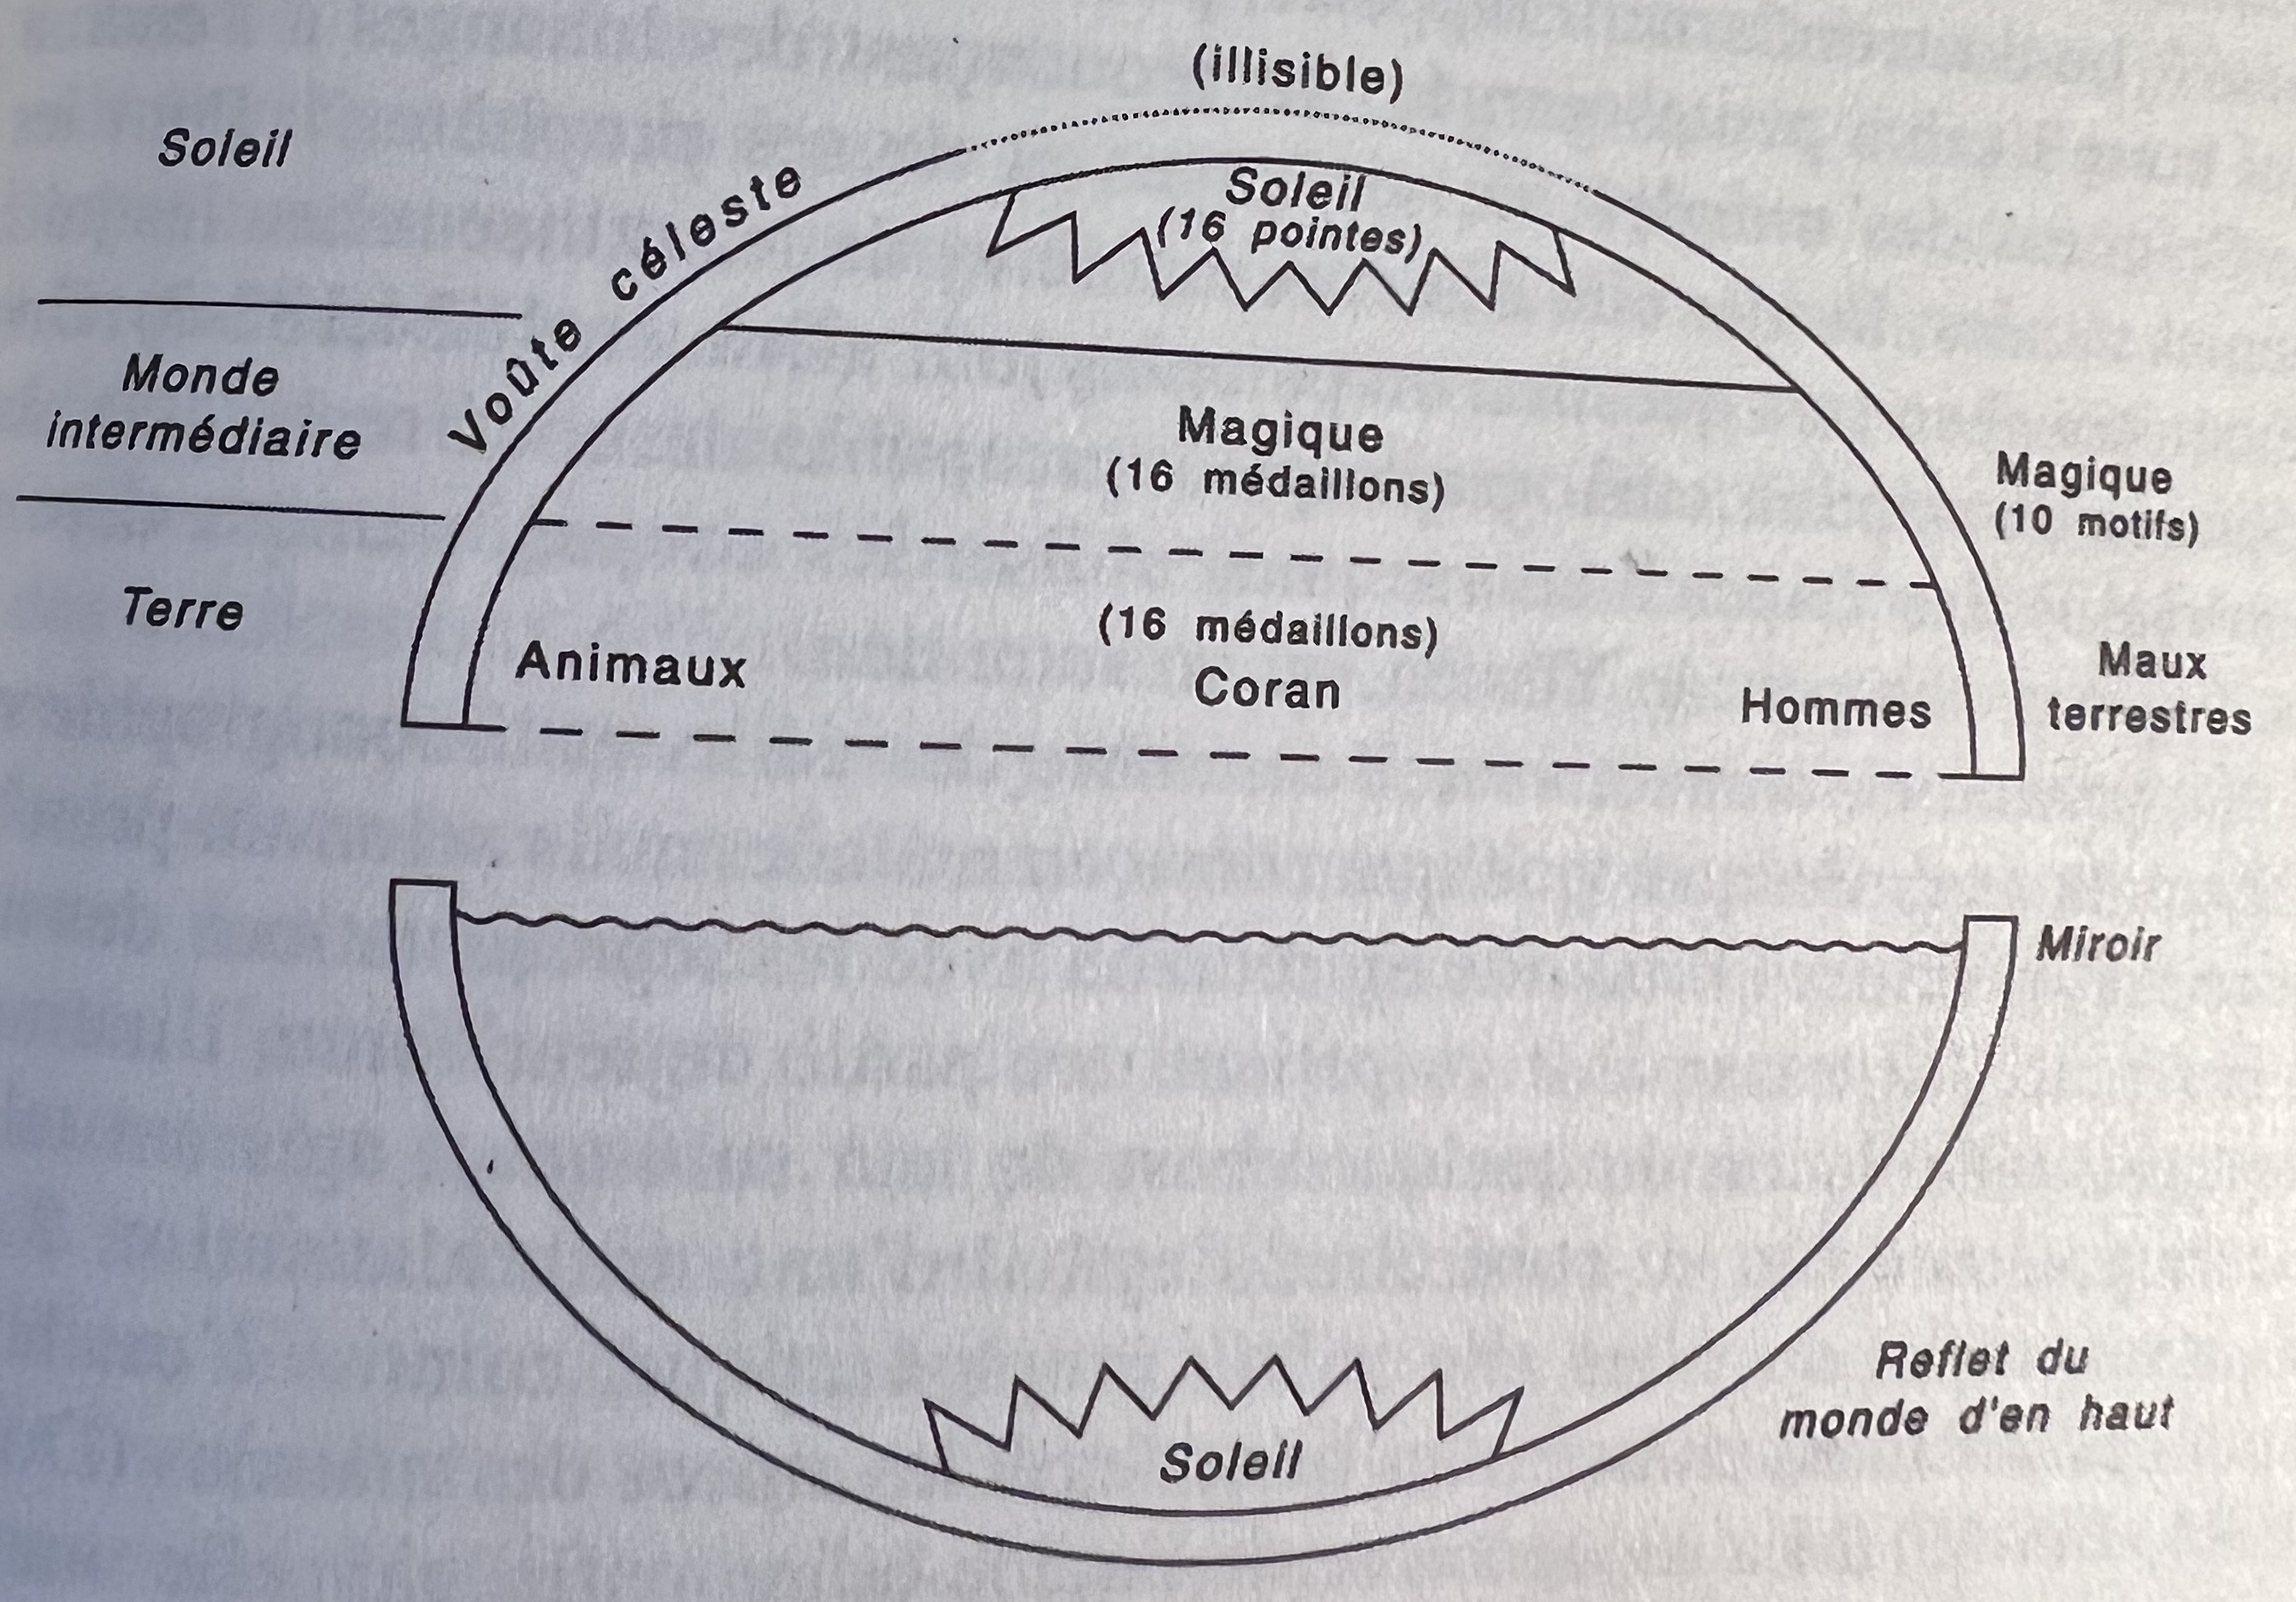
\includegraphics[width=0.7\textwidth]{HommeetIslam/Images/IMG_2459recadre.png}
   \caption{La Coupe comme représentation du cosmos. Coupe B paroi Interne et externe}
    \label{fig:my_label}
\end{figure}
 
\subsection*{Des biens d'une fondation pieuse - \textit{waqf}}
Après avoir étudié la coupe proprement dite, l'auteure étudie le statut particulier de ces coupes : elles sont la propriété d'une fondation pieuse, \textit{waqf}, depuis 1895. Pratiquement, il s'agit d'un \textit{waqf} oral, non enregistré auprès des autorités à la différence des biens immobiliers.
En étant \textit{waqf}, la légitimité religieuse est
renforcée. 
Mais ce qui retient l'attention, c'est le faible empressement de l'intendant de la mosquée envers les 2 coupes, dont il est pourtant le gestionnaire. Il les prête gratuitement quand on les lui demande mais il peut même douter de leur efficacité. Le pouvoir magique ne vient donc pas du propriétaire et de ses références magiques (à aucun moment la compétence magique n'est requise pour être responsable de mosquée) mais bien des coupes elles-mêmes,  du rite autour de ces coupes, ou de l'artisan qui les a fabriquées. Ceci est confirmé par le fait que de telles coupes étaient offertes en cadeau, au retour du pèlerinage à La Mecque (Canaan 1923, 130 \cite[note 63]{Regourd_2007}); la coupe (A) aurait ainsi été donnée en \textit{waqf} par un \textit{hâjjî}.

\subsection*{Utilisation des coupes}
L'enquête de terrain permet de décrire l'utilisation de ces coupes, en particulier dans le cas de grossesse difficile. 

\paragraph{Leur mode d’emploi consiste principalement à boire un liquide au contact de la coupe.}  Ce liquide - de
l’eau, du bouillon - ou le miel que l’on y a versé, est bu en disant des louanges à Dieu.
Le bouillon de viande est particulièrement prescrit pour les femmes en couches : par son pouvoir nutritif important (moelle,...), il présente des caractéristiques médicales intéressantes,  qui
viennent en addition de celles des écrits et représentations présents sur les coupes. 
\paragraph{La maladie est interprétée comme la conséquence de causes multiples.} Un tel recours simultané à plusieurs médecines différentes est courant dans la même région du Yémen. Il s'agit d'attaquer le mal dans toutes ses facettes. Lorsqu’il y a maladie,
elle est toujours soupçonnée d’être le résultat de causes multiples et la boisson dans la coupe est envisagée en complément d'autres actions, en fonction du diagnostic thérapeutique. De même, l’utilisation des coupes comme réceptacle de boisson n'est pas envisagée comme l'unique usage des coupes, comme le laisse penser les traces de bougie au fond de la coupe B. 


\subsection*{Historique des coupes}
Une coupe, même abîmée, conserve ses propriétés comme c'est le cas de la coupe B réparée plusieurs fois et qui a perdu une partie de ses écrits; le rite, nous l'avons vu, est des plus simples et ne semble pas complètement fixé. D'où vient donc le pouvoir magique de ces objets ? 

Il nous faut donc étudier l'origine de ces objets, que ce soit leur commanditaire ou l'artisan qui l'a fabriqué.

\paragraph{La titulature de Saladin présente sur les coupes est apocryphe.} Le commanditaire de ces coupes serait Saladin, une titulature clairement apocryphe et commune dans les objets magiques. Par une telle référence, la légitimité du pouvoir magique se trouve renforcée. 

 


\paragraph{Le rôle de l'artisan est secondaire.} Nous n'avons pas d'informations sur l'artisan mais l'étude des diverses coupes magiques montre des artisans différents, certains excellents, d'autres se contentant de copies mais toujours avec des variantes. 
Selon les mentions de certaines coupes, la puissance magique viendrait ou serait renforcée par la survenance d'un évènement astral lors de la fabrication de l'objet. Une telle mention, doublée parfois du nom d'un souverain,  ajoute par sa simple évocation, à la valeur et l'efficacité de la coupe.  
\paragraph{L'homme s'approprie la magie d'origine divine.} Nous avons vu que dans la vision coranique, la magie n'est pas innée pour l'homme.
Un mythe d’origine
des coupes véhicule l’idée que la copie peut avoir autant d’effet que
l’original. Les Palestiniens expliquent
ainsi l'origine des coupes : les bons anges en employaient de semblables
pour faire leurs ablutions. Ils en oublièrent un jour quelques exemplaires
à côté de la source où ils avaient 1'habitude de se rassembler pour se
laver. Un homme passant par là les trouva et s'en empara. Les propriétés
miraculeuses de la coupe furent bientôt découvertes. Des copies en furent
réalisées, qui manifestèrent les mêmes propriétés (Canaan, 1923,130;
1936, 127 cité par \cite{Regourd_2007})

 

 \subsection*{Conclusion}

\paragraph{La source de la magie semble l'addition de plusieurs facteurs } A la fin de cette étude, le pouvoir de ces coupes semble venir de l'addition de plusieurs facteurs et non d'un seul : mythe originel lié aux anges, titulature de Saladin, caractères magiques, formules coraniques adaptées, animaux et sceaux de Salomon, bien \textit{waqf}. 
De la même façon, son utilisation sera complétée d'autres approches thérapeutiques pour une approche que l'on qualifierait aujourd'hui d'\textit{holistique}.

\paragraph{L'anthropologie éclaire l'islamologie} En guise de conclusion, nous essayons de penser les conséquences de cette recherche anthropologique pour l'islamologie. Il apparaît de l'étude des diverses coupes que la magie n'est pas uniquement un élément exogène ajouté  à la foi musulmane mais fait du Coran une réalité bien plus riche qu'un simple livre à lire et à étudier, avec une lecture littérale du verset  : 
\begin{quote}
    Nous envoyons du Coran ce qui est une guérison et une miséricorde pour les croyants. (17:82)
\end{quote}
\vspace{1cm}
Développant ce verset, Winter peut conclure : 
\begin{singlequote}
    This healing
power of the revelation is understood literally by many, not just spiritually.
The qur’an was thus sometimes also used physically for curing [\ldots]. By means of amulets,
talismanic shirts and other artefacts covered with qur’anic inscriptions, often
in conjunction with astrological or magical devices or practices, the revelation
came to be put to all kinds of uses, not always strictly orthodox. By procedures reminiscent of the Cabbala, the letters of the Arabic alphabet and their
numerical values themselves played an important role in Muslim mysticism,
esotericism and the divinatory arts. \cite{winter_cambridge_2008}
\end{singlequote}
 
 
 
%\chapter{coupes divinatoires}


\paragraph{Coupe divinatoire} dit bol \textit{magique} en alliage de cuivre partiellement étamé, de forme circulaire aux bords évasés. La paroi extérieure est gravée d'une fleur de lotus à huit pétales calligraphiés au coeur en forme d'une étoile à cinq branches, et une longue inscription le long du rebord externe. L'intérieur est décoré d'un cartouche inscrit, de deux motifs de tughra, d'un sceau de propriétaire en forme d'amande «sahib Tador (Théodore ?) «et d'un cachet ARMENIEN daté 1875». Le rebord est gravé d'une longue frise épigraphique sur deux lignes. Empire ottoman, datée 1875.
Haut. : 4,9 ; Diam. : 15,1 cm

\includegraphics[width=\textwidth]{GénéralISTR/Image/bolsmagiques.jpeg}

\includegraphics[]{GénéralISTR/Image/Tughra_of_Abdülaziz 1861-76.jpeg}

\paragraph{fleur de lotus} Dans le bouddhisme, le lotus est associé à la pureté, à l’éveil spirituel et à la fidélité. La fleur est considérée comme pure car elle est capable de sortir des eaux troubles le matin et d’être parfaitement propre. Il est également connu pour symboliser la pureté de la parole, du corps et de l’esprit.


\paragraph{Bol talismanique ou bol magique} coupe de forme circulaire à bords évasés, ombiliquée en laiton anciennement étamé incrustation de pâte noire gravé à l'intérieur de mihrabs, inscriptions en écriture naskh\sn{Le naskh, aussi appelé naskhi ou neskhi  est le style d'écriture le plus répandu pour les langues utilisant l'alphabet arabe. C'est ce style que l'on apprend à l'école et que l'on emploie pour la calligraphie et l'écriture usuelle, manuscrite ou imprimée.} et nasta'liq\sn{Le nastaliq    est un des styles de la calligraphie persane, en alphabet persan, dont l'origine est attribuée à Mir Ali Tabrizi, originaire de Tabriz, au xive siècle} d'invocation religieuse et verset coranique, patine d'usage. Iran XIX-XXe.
Haut. : 4 ; Diam. : 13,5 cm




\paragraph{Duquoc} Nous nous trouvons là devant une ferme conviction : « Jésus ne se replie pas sur l’instant, il l’ouvre à sa profondeur », car le présent est « l’habitat de Dieu » (p. 113). L’auteur revient sur ce point avec insistance, comme pour surmonter le caractère paradoxal des affirmations du Christ, puisque si le Règne est là, le mal et l’injustice, eux aussi, semblent continuer de régner, inexorablement. La « tentation » est alors grande de vouloir faire coïncider le Règne présent avec la fin d’une histoire réconciliée qui dénie les réalités de notre histoire souffrante, en faisant appel à la magie, à la puissance messianique, à la conquête instaurant de force l’unité du Règne promis (comme le suggère le tentateur à Jésus au seuil de sa mission). L’Église n’a pas toujours résisté à cette tentation, comme on le voit lorsqu’elle cherche à dominer et à orienter la politique, illusion dénommée chrétienté (l’auteur développe ici sa réflexion en tirant profit du livre de Marcel Gauchet : La religion dans la démocratie. Parcours de la laïcité, Gallimard, Paris, 1998).  

\section{Dictionnaire sociologie religions}

 
 du prophétisme
Du latin divinatio, deviner, le terme « divination » désigne l'action qui se donne pour objectif de deviner, prévoir et/ou influencer
une réalité cachée, à l'aide de la lecture d'éléments, ou présages, selon une technique particulière impliquant leur observation ou leur manipulation. Ainsi définie, la divination apparaît comme une pratique universelle des sociétés  Les procédures divinatoires peuvent être motivées par diverses raisons découvrir les causes d'une maladie ou d'une infortune, retrouver un objet perdu, connaître les déterminations pesant sur l'avenir proche (dans le domaine de l'amour, du travail, etc.), être informé des circonstances propices à la réalisation d'une action ainsi que de ses chances de succès (départ à la guerre ou à la chasse, construction d'une maison, installation sur un territoire, etc.). La divination peut aussi être exécutée de manière quasi automatique, parce qu'elle est requise en telle circonstance par la tradition ou qu'elle fait partie intégrante d'un rituel. La divination est, soit explicative   et renvoie alors à des éléments passés, soit prédictive permettant de
connaître l'avenir de sorte à agir en consé-quence. Elle peut être réalisée pour le compte d'un individu, d'un groupe, ou d'un « bien » (du bétail, par exemple).
Les éléments qui servent de présages sont variés et leur lecture est susceptible d'être effectuée selon des procédés très divers : observations et/ou manipulations d'entrailles d'animaux sacrifiés, de vols d'oiseaux, de craquelures sur une carapace de tortue calcinée, de marc de café, de combinaisons d'objets lancés, de cartes, de présence de taches dans un jaune d'œuf, de l'emplacement des planètes, etc. Cette multiplicité des techniques s'illustre par la diversité des termes formés à partir de la racine grec \textit{mantiké} -divination-pour les désigner : chiromancie, géomancie, cartomancie, etc. La divination peut aussi être opérée sans autre support que le devin lui-même. Elle s'inscrit alors plutôt dans le domaine de la voyance : le devin établit un contact qui est dit direct -via les rêves, la transe ou la possession- avec des forces sur-naturelles. Mais si de multiples classifications des formes de divination ont été proposées formes ou techniques intuitives, inspirées, inductives, raisonnées..), aucune n'apparaît universellement pertinente, et il semble plus utile de se référer aux classifications indigènes
- les modes de divination étant généralement pluriels dans une même société.

En se fondant sur la combinaison, qui
nés à semble résulter du hasard, des éléments qui tion- servent de présages, la procédure divinatoire incie, manipule l'aléatoire pour mieux le dépasser.
si être
Une signification étant attribuée à chacune
 des combinaisons possibles. le hasard est   exclu de la trame des événements. L'incertitude qui motive la divination se trouve alors   intégrée dans un ordre intelligible et
  rassurant.
 
De ce fait, l'analyse des processus divins osées   informe sur les conceptions indigens
 , paraît
de la causalité. Les résultats de la divination
: plus peuvent renvoyer à un système de correspons
 
dances, permettant de penser que les procé
dures divinatoires relèvent d'un processus de rationalisation; elles activent un ordre dast licatoire et les systemes de correspondants


l'implique pas nécessairement, et le cours du destin peut toujours être plus ou moins « forcé ». Les processus divinatoires prédictifs servent d'ailleurs souvent à se prémunir contre un événement futur potentiel, voire à créer un autre futur : il est fréquent de recommencer une divination jusqu'à obtenir le résultat escompté, comme s'il s'agissait de mettre en place les conditions propices à la réussite de l'action que l'on souhaite entre-prendre. De ce fait, la divination intéresse les réflexions sur les processus de prise de décision et les théories de l'action. Entérinant certaines formes d'actions, elle œuvre comme une procédure de validation, ce qui la rapproche des systèmes juridiques.
La divination relève en fin de compte autant de l'individuel que du social. Elle est le résultat d'une interaction, impliquant au minimum le devin et son client, et généralement tout un pan de la société. En inscrivant le destin individuel dans un ordre englobant, les processus divinatoires font de l'individu un élément d'un système socio-cosmique qui le dépasse. Entre l'individu et le social, l'aléatoire et la détermination, l'interprétation et l'action, le religieux et le juridique, les processus divinatoires, variés dans leurs formes et leurs fonctions, touchent à de nombreux aspects de la vie d'une société, qu'ils permettent d'articuler.
• ADLER A. et ZEMPLENI A., Le Bâton de l'aveugle : divination, maladie et pouvoir chez les Moundang du Tchad, Paris, Hermann « Savoir », 1972. - CAQUoT A.
et LEIBOVICI M. (éds), La Divination, Paris, PUF,
1968. - EVANS-PRITCHARD E. E., Sorcellerie, oracles et magie chez les Azandé (1937), traduction ft. L.
\textbf{Evrard, Paris, Gallimard, 1972. - FAHD T., La Divination arabe: études religieuses, sociologiques et folkloriques sur le milieu natif d'Islam, Leyde, Brill, 1966.} \href{https://books.google.fr/books?id=ETsVAAAAIAAJ&lpg=PP1&hl=fr&pg=PA8#v=onepage&q&f=false}{La divination Arabe}
MAUPOIL B., La Géomancie à l'ancienne côte des esclaves, Paris, Institut d'Ethnologie, 1941, - PEEK P.-
M., African Divination Systems: Ways of Knowing.
Bloomington, Indiana University. Press, 1991.
VERNANT J.-P, VANDERMEERSCH L.. GERNET J., BOTTERO J. et al, Divination et rationalité, Paris, Seuil « Recherches Anthropologiques », 1974.
Grégoire SCHLEMMER
316



 
\section{Deux coupes magico-thérapeutiques, biens de fondation pieuse (Nord du Yémen) : transmission du savoir et efficacité}
 
Deux coupes magico-thérapeutiques (sing. \textit{tâsa}) sont dites biens de fondation pieuse ({\textit{waqf}}) d'une mosquée, à Sanaa. Elles appartiennent à une collection d'objets, tous ayant le même statut juridique et tous utilise à des fins thérapeutiques. La famille du responsable de l'intendance à la mosquée, a la garde de ces objets et doit les remettre à quiconque les réclame dans un dessein, bien sûr, thérapeutique. Le statut juridique précis de ces objets, inédit, soulève de nombreuses questions, et, en particulier, pour le domaine ici couvert, celle de savoir ce qui les rend efficaces.
Afin de me situer dans le cadre thématique de cet ouvrage, je me pencherai sur les différentes inscriptions, représentations et figures géométriques gravées sur les parois des deux coupes. Différentes réflexions sur l'usage et la fabrication des coupes en général, à partir des travaux existants, amèneront à se demander dans quelle mesure il est possible de parler de «coupes talismaniques ».
Cette étude a fait l'objet d'un terrain entre les années 1995 et 1998.
Nous ne disposons que de peu de descriptions de coupes se trouvant au Yémen ou ayant un lien avec ce pays, par rapport à la quantité d importante de travaux publiés sur ces objets.
\subsection{Description des coupes}


La première coupe A, hémisphérique, sans pied, à lèvre arrondie, réalisée dans un alliage cuivreux. La surélévation qu'on remarque en so centre semble résulter d'un choc. Ses dimensions, estimées d'après phote sont pour sa hauteur, de 7 à 8 cm environ, et pour son diamètre, de 15 16 cm environ*. Elle est antérieure à 1313/1895-96 (date de mise en \textit{waqf}). Elle porte sur ses parois interne et externe un décor incisé de façon assez sommaire, et a peut-être été rapportée du pèlerinage à La Mecque par son donateur.


Le décor de la paroi interne est organisé à partir du motif central qu'orne le fond de la coupe. Il présente deux carrés entrecroisés dont les hui pointes, prolongées à 45° par des droites, se rattachent à un cercle situé quelques centimètres de la lèvre, formant ainsi un motif structurant analogue à celui d'une roue. Au centre de la coupe, dans l'espace circonscrit par les deux carrés. se trouvent. gravés sur huit lignes, des bâtonnets, isolés les uns des autres et saturant l'espace. L'espace résiduel entre les pointes et les côtés des carrés est occupé par des marques, reprenant sans doute les bâtonnets. Huit médaillons occupent le registre intermédiaire, structuré par les pointes développées des deux carrés. On distinguera quatre médaillons, dans la moitié inférieure desquels figurent des représentations animalières et, dans la moitié supérieure, des bâtonnets, semblables à ceux qui viennent d'être décrits. Ces quatre médaillons alternent avec quatre autres, comportant des textes en arabe. Dans le premier type de médaillon, on parvient à identifier, en ce qui concerne les animaux représentés et dans le sens des aiguilles d'une montre, un scorpion (voir flèche fig. 1, coupe A), un chien, deux dragons affrontés (?), surmontés d'une bande ondulée, et un autre quadrupède (un cheval, un lion ?), avec au-dessus du dos un sceau de Salomon. Les bâtonnets « magiques ». quant à eux, sont chaque fois disposés sur trois lignes. Statistiquement, leur nombre est à peu près le même pour un médaillon donné : partant du scorpion et suivant le même sens, de la ligne supérieure à la ligne inférieure, on obtient le résultat suivant : 18/18/19 ; 19/19/17 ; 16/17/16 et 15/15/15. Quant aux textes des médaillons, en partant de celui situé entre le scorpion et le chien (?) et en allant dans le sens des aiguilles d'un montre, on parvient à déchiffrer :
\begin{itemize}
    \item (1) la \textit{basmala}, suivie de s84v1-4 (sourate « La déchirure », a
\textit{Inshigãq}), le 4° verset s'achève à : \textit{wa algat má fihà}, puis sur la ligne
les lettres \textit{kâf-râ'} (?), et, en dessous, sìn (?)-käf.
\item (2) dans le style d'une invocation (azîma) : « yâ Nüh, Banüh, Kali
(2), Kalükh, Kalkh, \textit{alif}-lâm-mim-ra' [lettres liminaires, sourate 13], alij lâm-mîm [lettres liminaires, sourates 2, 3, 29, 30, 31 et 32], \textit{alif}-lâm-min
ra' [ibid.], \textit{hâ}'-mêm-ayn-sîn-gaf [lettres liminaires, sourate 42], kâf-\textit{hâ}
ya'-ayn-sad [lettres liminaires, sourate 19], ta' (?), tâ'-\textit{hâ} [lettres lim naires, sourate 20], ta'-\textit{hâ} (?) », enfin dernière ligne, des chiffres (?).
\item (3) ???, des lettres séparées sur les deux dernières lignes : sìn-\textit{waw} (?
mim (?), ba', puis \textit{kâf}, ra' (?).
\item (4) ???, des lettres séparées sur les deux dernières lignes : shin-ra
\textit{hâ}'-ra', \textit{alif}, \textit{hâ} (?), puis \textit{alif}, hā'-ra' , \textit{alif}, dal, \textit{alif}.
\end{itemize}:

\includegraphics[width=\textwidth]{HommeetIslam/Images/IMG_2455.JPG}


Ces textes sont écrits pour trois d'entre eux sur sept lignes, un seul occupe huit lignes. Enfin, le registre compris entre la lèvre de la coupe le cercle auquel se rattachent les pointes des carrés, présente, aux extremités du cercle, 4 rectangles (façades de bâtiment, talismans?) alternant avec  4 formes cintrées (mihrabs ou stèles funéraires, amulettes ?). Ils contiennent les mêmes bâtonnets, arrangés sur des lignes, que les médaillons animaliers. Leur nombre est à peu près constant, dans les rectangles, entre 7 et 9 par ligne, dans les formes cintrées, entre 6 et 8 par ligne. L'espace entre ces motifs est occupé en alternance par des écrits magiques et de l'arabe, placés de façon à correspondre au style des écritures contenues dans les médaillons : les écrits magiques, au-dessus des écrits magiques et l'arabe au-dessus de l'arabe. A propos des écrits magiques, on relève systématiquement la présence d'hexagrammes ou sceaux de Salomon, suivis (dans le sens de l'écriture arabe, i. e. de droite à gauche) d'une série relativement stable de signes, de sorte que l'on a sensiblement quatre fois le même ensemble. Ces séries peuvent être assimilées à ce qu'al-Bûni appelle les sept lettres (\textit{al-ahruf al-sabr}), ou bien les
sept sceaux (\textit{al-khawâtim al-sab}°), ou encore \textit{al-tilsam al-Sulaymani}. 

Après le seau de Salomon, on relève successivement trois traits verticaux
surmontés d'un trait horizontal; la lettre \textit{mim} (parfois réduite à un trait sans véritable boucle, mais ce trait apparaît bien distinct des trois précédent reliés par le surlignage); deux traits verticaux, plus longs que les autre comportant deux barres obliques, qui les rendent analogues à des dièses (dans un cas sur quatre, les deux barres obliques n'apparaissent pas); quatre traits; pour conclure, une nouvelle étoile à six branches, mais aussi une sorte de y (?). La fin diffère de la série donnée par al-Bûnì, qui cite, après le quatre traits, les lettres \textit{\textit{hâ}}', puis \textit{wâw}. A moins de considérer, pour la coupe A, que la ligne qui clôt chaque série, et commence sur la ligne d'écriture revient vers le haut en s' incurvant et en direction des « lettres » précédentes ne soit un \textit{wâw} (Rehatsek, 1875b, 301, fig. 2). Chaque ensemble formé par ces « lettres » ou « sceaux » se trouve délimité par le cercle qui définit registre dans sa partie inférieure et par un surlignage plus ou moins contin qui rejoint le cercle en fin de séquence : chaque ensemble apparaît donc ins crit dans un cartouche. Le fait de délimiter un écrit porteur d'une puissanc magique est une pratique courante en islam arabe. Quant aux textes en arabe, on déchiffre : 
\begin{enumerate}
 
    \item   « La basmala, suivie de trois mots (?) ;   \item  \textit{wa ma
yatawakkal'ala Allah fa-huwa} (?) ;   \item  fa-huwa [une seconde fois ?] \textit{hasbuhu inna Alläh baligh amrihi;}
\item \textit{ wa al-salâh wa al-salâm 'alâ sayyidina Muhammad}
\end{enumerate}
Les textes 2 et 3 sont tirés de s65v3 (« La Répudiation », \textit{al-talâq}). La \textit{basmala} est liminaire et la prière adressée à Dieu en faveur du Prophète Muhammad, qui vient souvent clore un écrit, se trouve dans le dernier cartouche, suivant le sens de lecture de gauche à droite. Il peut donc s'agir d'une seule et même formule qui, déroulée sur le pourtour en 4 seg-ments, pourrait être lue perpétuellement. Cette coupe, dans sa composition interne, est, on le constate, largement construite selon le chiffre huit, souvent obtenu par l'utilisation de 4 fois 2 types d'éléments différents.
 
\includegraphics[width=\textwidth]{HommeetIslam/Images/IMG_2456.JPG}
La paroi extérieure comporte trois zones concentriques. Le fond de la coupe est occupé par un sceau de Salomon. Un premier anneau sur lequel s'alignent des bâtonnets est interrompu trois fois par des sceaux de Salomon, disposés en triangle. Un second anneau, situé dans la partie basse de la coupe, reprend le même système de bâtonnets et de sceaux, cette fois au nombre de quatre et disposés en carré. On dénombre ainsi huit sceaux de Salomon. Enfin, entre cet anneau et la lèvre, on relèvera deux lignes de texte. L'une, dont l'incision est plus profonde, se trouve gravée à proximité de la lèvre et s'étend sur tout le pourtour; elle indique :
 \begin{quote}
     « Hädhihi (2)\mn{Soit : « Celle-ci [i. e. cette coupe] [sert] pour la piga-re du serpent et du scorpion, les chiens enragés, à faciliter l'accouche. ment, aux saignements de nez, [pour les douleurs à] l'estomac ... (?), les coliques …. (?), un sceau de Salomon ... (?) »} li-lasat al-hayya wa al-agrab wa al-kalib (sic) al-kalib wo
li-usr al-walad wa al-ruäf wa al-miada ... (?) al-qawlanj ... (?) un sceau de Salomon ... (?) ».
 \end{quote}
 Deux traits verticaux avec une barre médiane séparent le début de la fin de la phrase. L'autre inscription, située entre celle-ci et le second anneau, est incisée plus profondément, le trait en est plus épais que la précédente. Cela suggère un rajout,
le texte le confirme : 
\begin{quote}
    « Waqafa \mn{[legs pieux du Häjj Husayn al-Hawa (?) à la mosquée, la protégée, en 1313/1895-96]} al-Hajj Husayn al-Hawâ (?) \textit{hâ}dhihi al-
tâsa (sic) alâ al-Jâmi al-mahrûs 1313 »
\end{quote}   La lecture du nom du donateur pose problème, car un \textit{alif} semble avoir été tracé à la suite du \textit{hâ}', puis un \textit{waw} gravé en partie sur le \textit{alif} et avec la marque d'un rattachement à une lettre qui le précèderait, mais qui n'est pas donnée; enfin de petites encoches semblent indiquer une volonté de raturer ce \textit{waw}.
Ensuite apparaît un signe ressemblant à deux \textit{waw}-s inversés dont les boucles s'entrelacent : il peut être identifié comme une marque de fin de phrase, à la manière des petits décors que l'on trouve dans les manuscrits.
La seconde coupe B, plus grande et plus ouvragée sur ses parois internes et externes au décor incisé, sans pied, à lèvre arrondie, a été réalisée dans un alliage cuivreux, et son fond, fendillé de manière semi-circulaire par l'usage, a fait l'objet d'une réparation. Il s'agit vraisemblablement d'une soudure. Ses dimensions sont de 6,5 à 6,6 cm de hauteur et de 18,3 cm de diamètre, mesuré de bord à bord extérieurs, la lèvre comptant pour 0,4 cm. Elle est de provenance inconnue. En ce qui concerne le décor de ses parois extérieure et intérieure, elle se rapproche d'autres coupes se référant à Abû al-Muzaffar Yûsuf (habituellement identifié comme Saladin), avec la liste de ses vertus curatives - il en sera question plus bas - mais s'en distingue, par l'absence de représentation de la Kaba en son centre (intérieur) (Savage-Smith, 1997, 73). Elle se rapproche davantage de quatre autres coupes, trois décrites par Rehatsek, et la quatrième, propriété du Science Museum à Londres. Elle n'est pas datée, mais à coup sûr fabriquée postérieurement à l'époque de Saladin,  semblablement entre le VIII-IX'/XIV°-XV° s. et le XII/XVIII, peut-être XIII /XIX s..

 \includegraphics[width=\textwidth]{HommeetIslam/Images/IMG_2457.JPG}

L'ensemble du décor de la paroi intérieure se répartit sur trois registres, chacun délimité par un double cercle. On a ainsi trois doubles cercles concentriques dont le dernier suit les contours de la lèvre. 
Le premier registre, constitué par le fond de la coupe et délimité par un premier cercle concentrique, est occupé par un écrit de type magique qui reste à décrypter'. On distingue autant que la détérioration et la réparation le permettent, des traits de hauteur inégale, des lettres de l'alphabet arabe. isolées, essentiellement \textit{hâ}', la (?), \textit{hâ} et \textit{kâf}, des chiffres, 6, 7, 95. Ils forment neuf lignes horizontales, la dixième suivant la courbure du cercle. Le second registre, situé dans la partie basse de la coupe, a essentiellement pour décor des bandes qui se chevauchent, formant seize pointes, une étoile à seize branches. L'espace résiduel est rempli d'écrits magiques, identiques aux précédents. Certains sont disposés sur le premier double cercle concentrique. Le troisième registre, enfin, occupe la plus grande surface de la coupe. Son décor est structuré par un motif de feuilles ou de pétales s'ouvrant en corolle, répartis sur deux hauteurs et décalés les uns par rapport aux autres. Ces « feuilles » forment autant de médaillons. La première série de médaillons, au nombre de seize, installée sur le second cercle concentrique, comprend exclusivement des écrits magiques identiques aux premiers, gravés sur six lignes, dont l'une est constituée par le second cercle concentrique. Quant à la série supérieure de seize médaillons, elle comporte, alternés, des représentations et des restes en arabe. On parvient à identifier les figures suivantes, dans le sens des aiguilles d'une montre : un soleil à huit rayons enfermé dans un cercle, un chien, un scorpion, un personnage (une femme avec un enfant, allaitant ?), un croissant de lune, un cheval, un serpent, un second personnage (personne mordue par un serpent ? ou possédée par un esprit malin ?). Autour d'eux, les mêmes écrits magiques, qui diffèrent cependant des précédents en ce qu'ils ne sont pas gravés sur des lignes.
L'ouvrage est fait de telle façon que la lune se trouve opposée au soleil, que l'un des personnages est dans l'axe de l'autre et les deux quadrupèdes face à face. En ce qui concerne les textes en arabe, il s'agit d'extraits du Coran, tous écrits sur huit lignes. En partant de la sourate liminaire, placée entre le chien et le scorpion, et en allant dans le sens des aiguilles d'une montre, on déchiffre :
\begin{enumerate}
   \item al-Fâtiha, jusqu'à
" .. ghayr al-maghdûb 'alayhim" ;
  \item précédée de la basmala, une partie de s25v45 (« la Loi ou la
Salvation », al-Furqân), jusqu'à "la-jaalahu sâkinan", enchaînée à s6v13
(« Les troupeaux », al-An'âm), enfin quelques 4 mots non déchiffrés;
  \itemla basmala, puis s84v1-4 (« La Déchirure », al-Inshiqâq), le verset
4 s'achève à : "wa algat má fiha", la fin reste à déchiffrer ;
  \item sans basmala, s24v35 (« La Lumière », al-Nür), jusqu'à « Júgad
min shajara mubâraka zaytâna là sharqiyya wa là [gharbiyya] », quelques lettres isolées (?), puis ra', les chiffres 7 et 2 ou 3
  \item la basmala, puis sur la 2° ligne, les 3 lettres liminaires apparaissant
au début de six sourates, celles de la Vache, d'al-'Imran, de l'Araignte, des Romains, de Lugmân et de la Prosternation (soit 2, 3, 29, 30, 31 er
32), à savoir \textit{alif}-lâm-mim, suivies de 3 mots non déchiffrés, puis sur la 3-ligne, les 5 lettres liminaires de s19 (« Marie », Maryam), à savoir \textit{kâf}.
hã'-ya'-ayn-sâd, suivies de quelques mots non déchiffrés, puis sur la 4. ligne, les 3 lettres liminaires du début de s26 et   28 (« Les poètes » et « le
récit », al-Shu'ara' et al-Qasas), à savoir tâ'-sîn-mim, enfin les autres
lignes n'ont pu être déchiffrées ;
  \item la basmala, suivie de deux lignes et demi non déchiffrées, puis viennent peut-être une partie de s16v69 (« Les Abeilles », al-Nahl),
« yakhruj min butûni\textit{hâ} sharâb mukht\textit{alif} alwânuhu fihi shif@' » (?), et une partie de s17v82 (« Le Voyage nocturne », al-Isrâ'), « wa-nunazzil
min al-Our'ân mâ huwa shifà »" (?) ;
  \item la basmala (?), puis on lit \textit{hâ}-\textit{alif}, lâm-\textit{hâ}' al-rahmân al-rahim), suivi de s8v62-64 (« Le Butin », al-Anf@l) : le dernier mot du v63,
« hakîm », n'est pas très lisible et le v. 64 est déchiffrable jusqu'à « hasbuka Alla », quelques mots restent ensuite à comprendre;
  \item) sans basmala, 2v255 (« La Vache », al-Bagara, « verset du
Trône », ayat al-kursi), jusqu'à : « ... là yuhîtûn »'.
\end{enumerate}

L'espace compris entre les médaillons et l'ultime double cercle est
occupé par les écrits magiques déjà rencontrés plusieurs fois. Sur le cercle supérieur de ce dernier double cercle, enfin, est gravée une rangée
des mêmes écrits. Le décor de la paroi extérieure offre trois registres. Le premier est constitué par le fond de la coupe qui laisse deviner, en dépit de l'usure, le même type de composition magique que sur la paroi intérieure; la forme géométrique qui l'enserrait a disparu. On reconnaît ensuite un cercle concentrique constitué encore des écrits magiques. Le second registre occupe la partie médiane de la coupe. Les écrits magiques sont cette fois inscrits dans cinq cercles et cinq trapèzes alternés. Enfin, le troisième registre présente une ligne d'écriture qui suit le bord de la lèvre et s'étend sur tout le pourtour. Elle est gravée de telle sorte que le début du texte s'enchaîne sans rupture avec la fin. Cette phrase ininterrompue pourrait tenir dans un double cercle concentrique : le graveur s'est appliqué à ne jamais en dépasser les limites invisibles et à emplir l'espace de telle sorte qu'elle donne l'impression d'une bande circulaire continue, très décorative. Elle est chargée d'indiquer les vertus curatives de la coupe, comme c'est le cas pour la coupe A24:
\begin{quote}
    « wa \mn{Soit : « Pour notre Seigneur, le Sultan, al-Malik al-Mujähid, le manda-victorieux Abû al-Muzaffar Yûsuf26. Y [la coupe] sont réunis des bienfaits éprouvés par l'expérience, elle [sert] pour les piqûres de serpent et de scorpion, pour la fièvre, la parturiente? et augmenter le lait, pour les morsures de] chiens atteints de la rage, pour les douleurs stomacales et les liques, la migraine et les élancements (?)?, pour conjurer les sortilèges, ou faire cesser le flux du sang, pour le mauvais œil et le mauvais sort  
pour empêcher la paralysie faciale et pour le rétablissement de la conscience des épileptiques (?), pour la dysurie, pour la réconciliation des adversaires (ou : les proches parents ?), pour les enfants agités. L'ensor-celé et celui qui est atteint, de même que la parturiente en difficulté (?), doivent [en boire le contenu par gorgées (?)].} li-mawlâna al-sultân al-Malik al-Mujähid al-muwakkal al-man.
sûr Abû al-Muzaffar Yasuf wa jumi a fiha manâfi mujarraba wa hiya li-
las'at al-hayya wa al-'agrab wa-li-al-hummâ wa al-mutlaga wa al-magh-
la wa li-al-kalb al-kalib wa li-al-maghass wa al-qawlanj wa al-shagiga
wa al-zarabân (?, sic) li-ibtâl al-sihr wa li-ramì al-dam wa li-al-ayn wa
al-nazra wa li-râd al-lawaga wa li-ifâdat al-masrû (?) wa li-usr al-baw!
wa li-sulh bayn al-aqrân (al-agrâb ?) wa li-nakad al-atfäl wa al- m.r: (?.
ou 'm.r.j?) bi\textit{hâ} al-mashür wa al-musâb wa al-bint (?) al-mu sira" ».
\end{quote}

\paragraph{Titulature de Saladin}
La titulature, la \textit{kunya} (= Abû al-Muzaffar) et le nom (ism = Yûsuf) (à
moins qu'il ne s'agisse que d'une kunya = Abû al-Muzaffar Yüsuf), mentionnés dans l'inscription, peuvent-ils servir à identifier le personnage ?

Et constituent-ils un élément fiable de datation de notre objet ? La même formule (sauf al-muwakkal) se retrouve chez Reinaud, sur les coupes n° 9420, chez Wiet, n° 14, chez Canaan - qui n'identifie pas - et surtout sur les deux coupes, dites de Saladin, étudiées par Zéki Pacha : « Izz li-mawlâna al-sultân al-malik al-mujâhid al-muayyid al-Mansûr Abû al-Muzaffar Yûsuf » et : « 'Izz. li-mawlânâ al-sultân al-malik al-mujâhid Abû al-Muzaffar Yasuf »». Les coupes dédiées à Saladin sont réputées nombreuses   mais ne sont pas nécessairement indicatrices d'un temps et d'un lieu de facture particulier. 
En effet, Wiet (1922, 319-28), dans un article très précis, critique la datation de Zéki Pacha en s'appuyant essentiellement sur des documents épigraphiques, mais aussi sur des chroniques : il montre que les inscriptions de ces deux coupes font entorse à la titulature de Saladin, et donc au protocole habituel, que ces formules sont rares au VI/XI s., et que les dates qui suivent la mention de souverains, sur les coupes, ne sont pas un gage de leur époque de fabrication; il concède toutefois que l'on puisse y voir une allusion au souverain ayyûbide - si l'on se rapporte à d'autres objets sur lesquels se trouve le même type d'anomalies - mais qu'en aucun cas, ces coupes ne peuvent être contemporaines de Saladin. Le style de la coupe B, de même que les conclusions de Wiet, font plutôt penser à une attribution posthume.

  \includegraphics[width=\textwidth]{HommeetIslam/Images/IMG_2458.JPG}
  \paragraph{coupe anti poison}
L'étude des écrits, représentations, signes et figures géométriques des deux coupes fait apparaître un registre commun avec la talismanique. La symbolique de la coupe A, telle qu'elle se dégage à partir des éléments décrits, vient confirmer certaines de ses propriétés curatives. Tout d'abord, il s'agit d'une coupe anti-poison ; al-Bânì cite une longue incantation (azima) versifiée, valable pour toute œuvre magique : elle décrit les sept lettres spéciales, rappelle qu'elles sont le nom suprême de Dieu, puis que moyennant l'ajout de lettres de la Torah, des Evangiles et du Coran, l'on sera protégé des serpents, scorpions et lions?. Il s'agirait donc, dans l'ensemble, des animaux nuisibles ou devenus dangereux dont la coupe guérit de la morsure ou de la piqûre. En outre, elle aide en cas d'accouchement difficile, ce qu'indique la présence de la sourate \textit{al-
Inshiqâq}. Des textes gravés sur d'autres coupes comparent le mouvement de la terre qui rejette ce qui est en elle et se vide, à celui de la femme qui met un enfant au monde dans des conditions favorables. Spontanément, les deux coupes m'ont d'ailleurs été présentées comme des « coupes pour l'accouchement », l'usage ayant probablement consacré cette fonction entre toutes. Selon al-Bûnî (s.d., (a), 91) encore, les trois bâtonnets, sans l'\textit{alif} sur le dessus, désigné simplement alors comme « protubérance » ou pointe de lance, et accompagnés du pentagramme, peuvent être employés pour guérir des maladies affectant l'intérieur du corps, dont les coliques (gawlanj), auxquelles fait référence la liste des maux soignés par la coupe
A. Enfin, les deux carrés entrecroisés gravés à l'intérieur de la coupe forment une étoile à 8 branches - cette étoile finissant dans un double cercle peut aussi représenter le soleil, dardant ses rayons? -. Décrite comme la gravure ou le diamant de l'anneau de Salomon, l'une de ses variantes se trouve sur les rouleaux magiques d'Ethiopie, où elle est appelée « sceau de Salomon »». Son centre, qui est également le centre de la paroi interne, est entièrement occupé de bâtonnets magiques. 
\paragraph{Pouvoir du roi Salomon - de son sceau}
Qu'il soit bague ou talisman, selon la Tradition, il donne à ce Roi son pouvoir sur les démons
-  pouvoir que le Coran lui reconnaît, dans la sourate Sâd, aux versets 34-39 - et donc sur la cause des maladies, ou tout au moins de certaines.
Dans certaines versions, il oblige les démons, qui sont des sortes de gardiens des maladies, à livrer les remèdes (Barkaï, 1996, 193). Dans l'ensemble, les démons - parfois appelés djinns - sont divisés en tribus liés à un habitat, et la maladie est ainsi territorialisée. Salomon n'éradique certes pas la maladie, mais, grâce à la puissance de son sceau, don du ciel, il est celui par lequel vient la guérison. On remarquera que le sceau de Salomon est gravé ici parmi les maux que la coupe est censée soigner.

Leur liste étant incomplète, on ne fera qu'évoquer les maladies spécifiquement provoquées par les djinns ou les démons que Salomon et ses formules peuvent exorciser. Pour ce faire, on doit s'asperger ou se laver avec l'eau versée dans la coupe. L'architecture de la paroi interne est ici toute conçue et rythmée à partir de ce motif. Elle est largement construite selon le chiffre huit ou ses diviseurs. L'étoile à huit branches et les huit étoiles à six branches, structurant les parois interne et externe, indiquent singulièrement qu'elle en appelle à la protection de Salomon par qui vient la guérison, les autres grands pourvoyeurs de guérison étant Dieu et le Prophète (évoqué dans la formule gravée près de la lèvre supérieure de la coupe A).


La coupe B présente également l'image des animaux à piqûre et morsure (scorpion, serpent, chien, cheval) et le début de la \textit{sourate de la Déchirure}. L'un des deux personnages (femme avec un enfant, l'allaitant ?) rappelle son pouvoir de faire venir le lait. La basmala, prononcée avant toute action et notamment avant d'ouvrir la bouche pour manger, de même que les Versets du Siège, appelés âyat al-hars wa l-hirz, protègent contre les mauvais dinns ou démons. C'est le cas également des cercles.
Thème que pourrait reprendre encore l'un des deux personnages (personne possédée par un esprit malin ?). Deux sourates renvoient aux sources de la guérison plutôt qu'elles ne visent une maladie en particulier. Le verset 69 de la sourate des Abeilles fait en effet allusion aux pouvoirs curatifs du miel, qui fait partie des liquides versés dans les coupes, selon mon informateur, et à absorber donc par les malades. Les vertus du miel sont extrêmement nombreuses et constituent un thème de prédilection de la médecine pronhétigue4) Par ailleurs. s17v82 (« Le Voyage nocturne »)
'une manière plus générale, s8v62-oulait, allaitant
) rappelle son pouvoir de faire venir le lait. La basmala, prononcée avant toute action et notamment avant d'ouvrir la bouche pour manger, de nême que les Versets du Siège, appelés ayat al-hars wa l-hirz, protègent contre les mauvais djinns ou démons. C'est le cas également des cercles.
Thème que pourrait reprendre encore l'un des deux personnages (person-ne possédée par un esprit malin ?). Deux sourates renvoient aux sources de la guérison plutôt qu'elles ne visent une maladie en particulier. Le verset 69 de la sourate des Abeilles fait en effet allusion aux pouvoirs curatifs du miel, qui fait partie des liquides versés dans les coupes, selon mon informateur, et à absorber donc par les malades. Les vertus du miel sont extrêmement nombreuses et constituent un thème de prédilection de la médecine prophétique*. Par ailleurs, s17v82 (« Le Voyage nocturne ») rappelle le pouvoir curatif du Coran. D'une manière plus générale, s8v62-64 (« Le Butin ») martèle l'idée que : « Dieu te suffit »*. Quant à la sourate liminaire, ses vertus sont tellement innombrables, qu'elle n'est plus indicative : elle est bonne pour tout. Enfin, les deux Luminaires, le soleil et la lune, sont des symboles de vie, de prospérité et d'abondance, comme le remarque Canaan (1936, 100, 121). De la même manière que les deux Carrés entrecroisés contenant des écritures magiques, à l'intérieur de la
«/iat (1932. 95-96. п° 3906. 121, л° 4431) : Сдатcoupe A, peuvent représenter le soleil sous la forme d'une étoile à huit pointes et qu'elle est structurée selon le chiffre huit, le soleil, dans la coupe B, compte également huit pointes. Par ailleurs, le fond de la coupe B est occupé par une étoile à seize branches, qui soutient sa composition interne en seize médaillons, puis en deux fois huit médaillons (à texte et à figures). Quelques coupes étudiées par ailleurs montrent une corrélation entre la présence des Luminaires et le chiffre 16 (cartouches ou cercles).
Le rapport est donc net entre le chiffre huit et le soleil. On est tenté de mentionner alors le fait que huit correspond à la valeur isopséphique du \textit{hâ}, lui-même clé de la vie (hayât), selon un procédé bien connu en science des lettres. Cependant, les versets des sourates 6, 24 et 25, gravés sur la coupe B, rappellent l'omnipotence et l'omniscience de Dieu, cause de tout et à qui tout doit revenir, au-delà des deux Luminaires : 
\begin{quote}
   « C'est à lui qu'appartient ce qui subsiste dans la nuit et le jour »; « Dieu est la lumière des cieux et de la terre ».
En guise de remarque finale sur les deux coupes, ne peut-on pas dire qu'elles consqu'appartient ce qui subsiste dans la nuit et le jour » ; « Dieu est la lumiè re des cieux et de la terre ». 
\end{quote}

\paragraph{Cosmos}
En guise de remarque finale sur les deux coupes, ne peut-on pas dire qu'elles constituent une tentative de reproduire le monde clos du cosmos ?

\includegraphics[width=\textwidth]{HommeetIslam/Images/IMG_2459.JPG}



En effet, le soleil qui préside à l'architecture interne des deux coupes, les cercles concentriques, les entrelacs de rubans ininterrompus, les textes eux-mêmes parfois écrits de telle manière qu'ils ne s'achèvent ni ne commencent, les motifs alternés qui se répondent, ainsi que la concavité et le caractère hémisphérique des deux objets (Canaan, 1936, 82), sans compter la composition organisée en registres, concourent à le reconstituer, quelques sourates rappelant que Dieu demeure Le plus puissant, Le plus savant et la Cause unique et suprême. Si l'on songe que le mode d'emploi des coupes consiste à passer par un liquide qu'on y verse, celui-ci se trouve donc en contact avec toute chose du monde : ambition holistique des coupes.Le recours aux coupes thérapeutiques est d'un usage bien établi au
Yémen, aussi bien dans la communauté juive que musulmane (Brauer, 1934, 182-3)47, surtout dans les cas d'accouchements difficiles ainsi que, concurremment à d'autres pratiques, contre le venin des serpents. L'acte de soigner différents venins, parmi lesquels celui des scorpions, est particulièrement investi par diverses médecines ou pratiques. C'est sans doute un indice de la fréquence du danger. Selon l'un de ceux qui ont la responsabilité des coupes à la mosquée, leur mode d'emploi consiste principale-328
nent à boire le liquide - de l'eau, du bouillon - ou le miel que l'on y a versé". Le docteur Sarnelli rapporte, pour le Yémen des années 30, qu'il aut boire l'eau à petites gorgées en prononçant des louanges à l'endroit lu Seigneur des mondes, de ses anges et de ses prophètes. Pour les nêmes années, Brauer cite d'autres manières de les utiliser chez les juifs éménites, il en sera question un peu plus loin (Brauer, 1934,182-3). Une éritable description ethnographique, susceptible de nous renseigner sur ensemble des étapes à suivre pour utiliser les coupes, manque cepen-ant, que ce soit pour le Yémen, ou un autre lieu.
Le produit en contact avec l'ensemble des écrits et l'iconographie est hargé de communiquer quelque chose au malade, mais selon un principe ui reste à définir. Le liquide en relation avec les représentations des ani-aux nuisibles transmet-il au patient une partie de leur force, l'immuni-int par assimilation de quelque chose de leur substance, agissant tel un intrepoison ? Ou au contraire, s'agit-il d'une mithridatisation ? Les présentations ont-elles une valeur prophylactique, comme c'est le cas ur des talismans chassant les bestioles et les chiens des maisons (Doutté.
194, 144-46) гdant, que ce soit pour le
Le produit en contact avec l'ensemble des écrits et l'iconographie chargé de communiquer quelque chose au malade, mais selon un princi qui reste à définir. Le liquide en relation avec les représentations des a maux nuisibles transmet-il au patient une partie de leur force, l'immu sant par assimilation de quelque chose de leur substance, agissant tel contrepoison ? Ou au contraire, s'agit-il d'une mithridatisation ? I représentations ont-elles une valeur prophylactique, comme c'est le pour des talismans chassant les bestioles et les chiens des maisons Dou 1994, 144-46) ? La séquence écrits-liquide-boire, enfin, rappelle une p ique présente dans l'ensemble du monde arabe, qui consiste à écrire in papier, à l'encre noire ou de couleur, généralement des versets ce riques, et à le tremper dans un récipient empli d'eau, que l'on demande nalade de boire, notamment dans les cas d'ensorcellement!.
Cependant, dans le contexte yéménite des hauts plateaux, il sem! ue le bouillon versé dans les coupes serve à soutenir plus spécialem s femmes en couches??. Le bouillon de viande (marag) est gras, robotif, et rassemble la substantifique moelle de la viande : il est offert en début de repas et particulièrement aux hôtes, comme un met prisé et recherché, le meilleur en somme. Il est par conséquent indiqué pour soutenir physiquement la femme en travail. Ici, le liquide n'est donc pas seulement conducteur ou à la rigueur stimulateur, dans l'économie de la guérison par les coupes, mais il apporte ses vertus propres, qui viennent en addition de celles des écrits et représentations. En médecine domestique, pour la même région du Yémen, le recours simultané à des médecines et à des médications différentes est courant. Plutôt que le reflet d'un tâtonnement thérapeutique, il faut y voir au contraire un discernement et la volonté d'attaquer le mal, dans son éventuelle pluralité, dans toutes ses facettes. Les symptômes sont en effet soigneusement observés et triés, et, à partir d'eux, il s'agit d'évaluer les causes, qui peuvent être diverses pour un même symptôme. Symptômes et causes ne peuvent être tous traités de la même manière, et entraînent la décision de recourir à tel ou tel praticien. En outre, lorsqu'il y a maladie, elle est toujours soupçonnée d'être le résultat de causes multiples, de nature diverse, déchaînées en même temps. L'utilisation des coupes, dans le cas qui vient d'être évoqué, n'est clairement pas un acte médical unique.
Des traînées de bougie apparaissent au fond de la coupe B. Sont-elles en rapport avec l'utilisation des coupes ? Enfin, on observera que la coupe B, réparée, est toujours considérée comme en service. Pourtant, les détériorations et les réparations ont entraîné, pour partie, la disparition du décor gravé au fond.Institutionnalisation de pratiques magiquesQue ces objets soient wagf et non milk ne fait aucun doute pour leurs gardiens. On trouve d'ailleurs gravé sur la paroi externe de la coupe A, à la suite de la liste de ses propriétés, l'indication suivante: « Wagafa al-
Hajj Husayn al-Hawâ (?) \textit{hâ}dhihi al-tâsa (sic) 'alâ al-Jâmi al-mahrûs
1313 » [legs pieux (wagf) du Häjj Husayn al-Hawa (?) à la mosquée, la protégée, en 1313/1895-96]. Outre l'intérêt immense d'avoir ici une date, certes tardive et à ne pas prendre pour une date de fabrication, on retiendra qu'un tel statut pour un tel objet est bien un fait. Et le cas qui nous occupe n'est peut-être pas singulier. L'une des coupes signalées par
Ahmed Zéki Pacha, provenant du Bimâristân al-Mansär - du nom de son
fondateur al-Malik al-Mansûr Qalâwûn, en 683/1284, au Caire - et encore en service à la fin du XIX s., permet sans doute de ne pas limiter
au Yémen zavdite. L'ensemble des instruments utilisesl'hôpital était en effet considéré comme wagf. Cependant l'établisse. ment du statut juridique des objets qui nous occupent, pose problème.
Tout d'abord, ils ne seraient pas recensés par le registre des wagfs. Il est difficile de croire à une négligence d'autant que leur qualité de bien wagf n'est pas dissimulée. En 1998, dans une ambiance peu favorable il est vrais, la tentative de consulter ces registres du Ministère des wagf-s a tourné court. Mais aux alentours de 1999, les objets semblent avoir été récupérés par ce même Ministère, selon ce qu'a révélé une nouvelle visite au lieu où ils étaient auparavant déposés. Jusque là, ils semblaient échapper au contrôle de l'administration des \textit{waqf}-s et à toute redevance.
Ils m'ont été présentés comme « wagf-s oraux ». La procédure paraît connue et rodée. Le donateur vient et dit au récipiendaire : « Je donne cet
objet en \textit{waqf} à la mosquée [awgaftu \textit{hâ}dha al-shay' alâ Jâmi kad\textit{hâ} ».
Et voilà tout. Elle est adoptée pour des objets isolés, tels les corans, les tapis, offerts à la mosquée par des particuliers, musulmans, et qui ne représentent ni de grosses quantités, ni sans doute une valeur à l'unité très importante : dans ce cas, le principe de l'absence de tout document fixant destinataires et frais de gestion (wagfiyya), de même que l'absence de démarche d'enregistrement au Ministère des wagf-s, sont admis et connus du même Ministères. Certains d'entre ces objets, tels les coupes, le Livre, ou tout ouvrage en général, peuvent porter - mais pas nécessairement - une inscription mentionnant qu'ils sont biens wagf, d'autres non, tels les tapis. Il existe des tampons pour les ouvrages, usant de formules consa-crées, où le donateur peut ajouter son nom%. En somme le message est suffisamment clair : la mise en wagf de ces objets signifie essentiellement qu'il est interdit à quiconque de les utiliser à des fins personnelles et de
les vendra
une inscription mentionnant qu'ils sont biens wagf, d'autres non, tels les tapis. Il existe des tampons pour les ouvrages, usant de formules consa-crées, où le donateur peut ajouter son nom*. En somme le message est suffisamment clair: la mise en wagf de ces objets signifie essentiellement qu'il est interdit à quiconque de les utiliser à des fins personnelles et de les vendre.
Si les avoirs transmis sont clairement ici les objets, dans les faits, on ne voit pas bien en revanche comment se fait la prise en charge de leur entretien et, pour ceux qui nous concernent, des frais entraînés par l'accueil des demandeurs. En effet, ils suscitent des dépenses - même si on peut estimer qu'elles sont infimes - et pas de revenus. Nos quatre
objets sont prêtés sur simple demande, sans contrepartie d'argent, afin que même les plus démunis puissent se soigner. Autrement dit, ils génèrent plutôt du bien ou un service, du fait de leur usage thérapeutique (l-al-khayr). D'un autre côté, ils ont besoin d'être entretenus et réparés : les coupes se perforent par usure - c'est le cas de la coupe B, et il n'est pas rare de trouver des coupes dont le fond est percé - le manche du miroir a été soudé à la partie centrale et cette soudure peut se détériorer, enfin, la pierre risque d'être attaquée par le venin. Quant au destinataire, il s'agit de la mosquée, l'inscription de la coupe A le dit explicitement. Toute personne malade ou envoyée pour un malade et même si elle n'est pas du quartier ou de la Vieille ville, peut emprunter ces objets. Sur ce point, les dispositions légales ne font que reprendre un usage bien établi, en ce qui concerne les coupes tout au moins. Car même en propriété privée, elles ont toujours été prêtées à la demande et elles ne mentionnent dans leurs inscriptions aucun destinataire en particulier pour qui elles auraient été fabriquées, j'aurai à y revenir plus loin. De plus, l'usage collectif ancestral des coupes trouve parmi les catégories connues des fondations pieuses, sa case légale : il relève des fondations « d'orientation publique
ou charitable (wagf khayrt) » (Deguilhem, 1995, 16).
Au regard encore de la définition d'une fondation pieuse, de son principe même, le cas qui nous occupe demeure problématique ou inédit, si
Cas gla dent l°obiet d'un écrit chargé de fixer les modalitéstral des coupes louve parmi les categones connues des fondations pieuses, sa case légale : il relève des fondations « d'orientation publique
ou charitable (wagf khayrt) » (Deguilhem, 1995, 16).
Au regard encore de la définition d'une fondation pieuse, de son principe même, le cas qui nous occupe demeure problématique ou inédit, si tout wagf fait normalement l'objet d'un écrit chargé de fixer les modalités par lesquelles des revenus seront alloués à un (ou plusieurs) destinataire(s) (Deguilhem, id, 15). En ce qui concerne des dispositions particulières, force est de constater que le Yémen a fait l'objet de peu d'études, aussi bien en langue arabe qu'en langue européenne, sur les diverses modalités de fondations pieuses y ayant cours; il reste donc relativement méconnu sur ce points
Il est encore possible de se reporter à la transmission orale, si l'on veut tenter de préciser la provenance et la date à laquelle ces objets ont acquis leur statut. En se plaçant du strict point de vue de la collecte des données, les informations restent imprécises et contradictoires, liées aux souvenirs de chacun et à l'ancienneté de leur présence dans ces lieux. Sur les quatre objets concernés, l'un était propriété du QQ'im actuel : c'est lui qui l'a donnée en wagf à la mosquée. D'après ce dernier, les trois autres objets bénéficient du même statut depuis très longtemps, puisque non seulement il les a toujours vus, mais ils sont là depuis plusieurs générations, si l'on se fie au témoignage de son grand-père. Tandis que son fils déclare que la332
CORAN ET TALISMANS
coupe A n'est devenue wagf de la mosquée que depuis six ans [données de 19951 : elle était auparavant la propriété d'un membre de la famille, habitant hors de Sanaa, sans pourtant qu'il puisse préciser où (la mention de bien waaf, gravée sur la coupe A, n'indique pas plus de lieu). Au terme de la discussion, une solution est finalement proposée, qui intègre les divers épisodes. Elle consiste à dire que la coupe a été volée par les tribus entrées dans Sanaa lors de l'assassinat de l'Imam Yahyâ, en 194858 ; puis qu'elle a été restituée, sans autre détail sur les péripéties. Il est vrai que ces coupes magiques sont considérées comme des objets précieux (tuhfa).
Finalement, les désaccords entre les informateurs ne portent à aucun moment sur le statut légal des objets. L'information substantielle à retirer d'un point de vue ethnologique concerne, semble-t-il, la perception reçue des hommes de tribu, chez les citadins : selon eux, ce sont des pilleurs, susceptibles de s'emparer de biens wagf-s et, au total, ils représentent des responsables idéals, pour ne pas dire miraculeux.
Au total, ces quatre objets sont des biens donnés par des particuliers en wagf khayri à une mosquée, sans wagfiyya, i. e. d'acte fixant en particulier par écrit leur gestion, dans le cadre des modalités de répartition dessusceptibles de s'emparer de biens wagf-s et, au total, ils représentent des responsables idéals, pour ne pas dire miraculeux.
Au total, ces quatre objets sont des biens donnés par des particuliers
en wagf khayri à une mosquée, sans wagfiyya, i. e. d'acte fixant en particulier par écrit leur gestion, dans le cadre des modalités de répartition des revenus; ils n'apparaissent pas non plus dans les registres du Ministère des \textit{waqf}-s. On peut cependant se demander si ce statut légal avéré ne représente pas par ailleurs une « solution » intéressante étant données le relations conflictuelles entre ce Ministère et ses administrés, et si elle n'est pas une modalité de la résistance, par ex., à une mainmise sur les fondations pieuses, sans même supposer de position idéologique. De plus la coupe A a un itinéraire compliqué, dont la traçabilité ne semble par toujours claire, et n'est « sauvée » de ses lacunes que par des solution pour le moins providentielles. Quoi qu'il en soit, l'inscription gravée su la paroi externe de la coupe A atteste que la mise en \textit{waqf} de ce typ d'objet est séculaire. Son statut juridique est de la sorte officialisé, rend public. Depuis plusieurs générations, aucun interdit majeur ne pèse don sur la pratique qui consiste à rendre un tel bien fondation pieuse et àrattacher à une mosquée. C'est pourquoi, on parlera ici d'institutionnalisation d'une pratique magique.Transmission du savoir et efficacitéLa responsabilité de la « gestion » des quatre objets magiques, en tant que biens wagfs, dépend du systeme régissant la succession à la charge suprême, dans la mosquée concernée. C'est, en l'occurrence, aux représentants de la même famille qu'échoit le titre de Mudir al-Jami depuis des générations*. Hériter de cette responsabilité n'est à aucun moment lié au fait de posséder un savoir en magie. Cela laisse planer la possibilité d'un divorce entre le responsable, ses références, ses convictions personnelles d'une part, et la nature des objets, son devoir de les prêter, d'autre part.
C'est précisément le cas à propos d'un autre objet déposé en wagf : l'un de ses « gardiens » doute de ses vertus magiques, même si cela n'engage pas nécessairement son opinion sur les coupes. Ses critiques sont formulées d'un point de vue rationnel. Le mode d'emploi des coupes semble de plus largement connu??, D'autre part, le statut de wagf khayri de ces deux coupes impose un usage non privé et non personnel. La manière d'utiliser les objets qui nous occupent est-elle alors ou non représentative d'une pratique ou d'une tradition et en définitive sur quoi repose l'efficacité des coupes ?
Si l'on se rapporte aux travaux antérieurs sur les coupes, il apparaît qu'elles sont la propriété de particuliers ou de familles dont rien n'indique un rapport particulier avec les pratiques magico-thérapeutiques. Regardées aussi comme des objets précieux, elles appartiennent au mobilier d'illustres familles et, à ce titre encore, elles figurent dans les Musées* : certaines334
sont des pièces d'orfèvrerie, fabriquées à partir de matériaux nobles, et leurs vertus leur confèrent en outre de la valeur. Elles sont habituellement prêtées à ceux qui les réclament - en principe le malade ou une personne depêchée par lui, et non un praticien - sur leur simple demandes. En effet, le mode d'emploi ne semble pas nécessiter la présence d'un prati-cien. Lorsqu'il est gravé et indique les maux soignés par la coupe, seuls le liquide à y verser et la manière de l'utiliser (boire à petites gorgées, asper-ger, etc.) sont spécifiés (Canaan, 1936,125-26). En outre, à défaut cependant de véritable étude ethnographique, les rares relevés ne mentionnent pas davantage l'existence de praticiens®. Néanmoins, l'étude ethnologique d'Erich Brauer sur les juifs yéménites, qui a l'avantage de donner une chaîne un peu plus complète d'opérations, mentionne le rôle de l'accoucheuse : la femme aidant à l'accouchement (mahjeräh) emprunte une coupe, qui a déjà donné de bons résultats, aux riches familles connues pour en posséder une ; elle la pose alors sur le ventre de la parturiente pour faciliter l'accouchement. S'y ajoute, le cas d'une praticienne juive yéménite qui exerce au Nord du Yémen et que je n'ai pu observer.
En dehors de ces exemples notables, on ne relève en général pas d'intervention d'un intermédiaire reconnu pour ses compétences en magie ou, en tout cas, pour soigner avec ce type d'objet.qu'elles ne sont pas réservées à un utilisateur particulier - de même que dans notre cas de wagf khayr? - et, sauf exception, elles ne mentionnent aucun nom de propriétaire ou de destinataire pour lequel elles auraient été spécialement fabriquées, Sur ce point, elles se distinguent des coupes araméennes et de certains bols arabes en poterie, employés dans les années 30, qui portent le nom du malade et celui de sa mère, suivant des pratiques talismaniques encore très répandues en monde arabe et subsaha-rien (Canaan, 1936, 80, 123-4). Le rapprochement avec les talismans qui sont imprimés et vendus dans des boutiques en monde arabo-musulman, tel le fameux Sab "uhād Sulayman, est tentant, mais une fois utilisés par son acheteur, peuvent-ils être empruntés par tout autre ? Les deux coupes, objet de cette étude, sont donc représentatives dans l'ensemble, car d'un usage collectif qui ne suppose, à aucun stade de leur emploi, le concours d'un homme de magie.
L'efficacité des coupes reposerait-elle alors sur leur fabrication par un homme de magie ? Quelques travaux des années 20 et 30 en font une spécialité de Persans, dont les ateliers auraient été soit en Perse, soit à La Mecque". Annette Ittig, s'appuyant sur le fait que le nom du destinataire-propriétaire n'est pas spécifié sur les coupes, avance qu'elles peuvent être fabriquées par des ateliers ayant une forte productivité, et l'existence de copies médiocres vont dans le sens de cette observation (Ittig, 1982, 94 ;
Canaan, 1936, 117). Mais 19 des coupes déjà publiées se réferent à un événement astral sous les auspices duquel elles auraient été gravées".

volt repor-
te sur les coupes, et lorsque c'est le cas, il n'est pas toujours identifiable comme persan ou/et astrologue ou homme de magie". En outre, sur les 19 coupes mentionnant un événement astral, 13 donnent à la suite une (pseudo ?)-date de fabrication, et sur ces 13, 8 sont « datées » du VICXII's.
On sait déjà que la date de l'une de ces coupes est problématique, car supposée être gravée lorsque la lune était en Scorpion, en l'année
570/1174-75, pour al-Mansûr Asad al-Din Shirkuh, l'oncle de Saladin : or, Shirkuh est mort en 564 H'. Enfin, l'événement astral est parfois évoqué par des formules quasiment identiques. A-t-on affaire à un phénomè. ne historiquement situé, qui consistait à vouloir placer l'efficacité des coupes sous le signe ou l'influence d'un événement astral, sans vraiment en maîtriser la connaissance ? Il est clair, en tous les cas, que l'on a affaire pour partie à des copies, même si - c'est très important de le souligner
- aucune des coupes publiées n'est identique, de même qu'aucune de celles que j'ai vues. Les artisans apparaissent donc comme chevronnés, car capables d'introduire des variations tout au moins dans l'architecture du décor, et certains ont eu éventuellement des compétences en talisma-nique; on songe moins à des praticiens de la magie auxquels aurait été confié le soin de graver. L'étendue de leur savoir (religion, astrologie, magie,.) et de leur technique peut être exceptionnel, mais certains imi tent les motifs, en particulier magiques, sans plus en avoir la clé. Cela signifie que même dans le cas où les inscriptions des coupes aiguillent sur l'existence d'hommes de magie au moment de leur fabrication, cela n'est pas toujours le cas. Enfin, dans l'hypothèse où les formules se référant àun événement astral auraient été copiées, doit-on penser qu'il s'agit simplement de faux ? Ne faut-il pas plutôt considérer que l'artisan procédait ainsi parce que la simple évocation de l'événement astral, doublée parfois du nom d'un souverain, ou rapporté à l'époque de Saladin, venant en addition des écrits et motifs gravés sur la coupe, ajoutait à la valeur et à l'efficacité de la coupe (Savage-Smith, 1997, 73) ? Certains textes gravés sur les coupes, ne laissent aucun doute sur le fait qu'être une copie, représente une valeur ajoutée. D'après Canaan, les Palestiniens expliquent ainsi l'origine des coupes : les bons anges en employaient de semblables pour faire leurs ablutions. Ils en oublièrent un jour quelques exemplaires à côté de la source où ils avaient l'habitude de se rassembler pour se laver. Un homme passant par là les trouva et s'en empara. Les propriétés miraculeuses de la coupe furent bientôt découvertes. Des copies en furent réalisées, qui manifestèrent les mêmes propriétés (Canaan, 1923,130;
1936. 127)
 Comme au premier jour, selon ce récit, la coupe abandonnee puis reproduite conserve son pouvoir.
Il viendrait alors principalement des écritures et figures gravées qui le communiquent au malade par le biais d'un liquide absorbé, aspergé, la surface la plus investie par cet ensemble de signes restant l'intérieur des coupes". Il faudrait également compter avec les propriétés des différents métaux utilisés, généralement le bronze et le cuivre jaune. Mais si le liquide versé varie en fonction du mal, il ajoute ses propres vertus à l'opération et l'eau elle-même possède ses propriétés particulières" : à preuve, la recherche d'une eau « plus active ». Canaan mentionne que le en fin d'operation
souvent par l'indication que les coupes sont eprouvées (« \textit{hâ}dhihi al-tasa mujarraba »), plus rarement par une « garantie » de qualité, en tant que copies, sans doute d'originaux réputés. Certaines coupes sont reconnues nettement plus efficaces que d'autres, telle celle dédiée à Salâh alDin (Zéki Pacha, 1916,254), ou comme Brauer l'a relevé. La répétition d'une formule ou la multiplication d'un même type de sentence, des versets par exemple, voire l'ancienneté des coupes y contribue®. Pour finir, la présence de ces objets dans la mosquée leur confère certainement un pouvoir supplémentaire auprès des utilisateurs. Cette remarque va, du reste, dans le sens de certaines inscriptions figurant sur les coupes, qui soulignent qu'elles ont été produites à La Mecque ou pendant le mois de Ramadân.
En résumé, les coupes sont généralement utilisées sans qu'œuvre un homme de magie ou quelqu'un qui, à des degrés divers, aurait des notions de magie. Elles sont d'usage collectif, elles ne sont en principe pas fabriquées pour un destinataire en particulier. De ce point de vue, les deux coupes, objet de notre étude, peuvent donc être ramenées au cas général.
Quant à la fabrication des coupes en général, nous savons encore fort peu sur leurs artisans. Cependant même dans les cas où les inscriptions sur les coupes évoquent le recours à une astro-magie, il peut s'agir de la simple référence à un événement astral, sans rapport certain avec le moment de leur fabrication. On ne peut en induire d'emblée que l'artisan a effectivement eu des notions de magie ou d'astrologie. L'efficacité des coupes guérisseuses serait donc intrinsèque en ce sens qu'elle ne supposerait pas nécessairement le concours d'un homme de magie.
\section{Du magico-thérapeutique}
Le rapprochement entre les écrits, représentations, signes, et figures géométriques apparaissant sur les parois des coupes et les talismans a339
déjà été fait, non seulement par des études, mais il est aussi bien attesté par l'inscription suivante gravée sur certaines coupes : « Hadhihi al-tilas-mât etc. ». L'expression, au pluriel, semble bien désigner en effet ce qui est gravé sur leurs parois%.
À notre connaissance cependant, aucune dénomination vernaculaire ne désigne les coupes elles-mêmes comme talisman. D'autre part, les spécificités que l'on vient de dégager, à savoir que les coupes ne font interve-nir, généralement, aucun praticien dans leur mode d'utilisation, qu'elles ne sont pas fabriquées pour un destinataire nominalement désigné, qui en aurait besoin pour résoudre un problème précis et pour son usage particu-lier, et enfin, que l'on constate largement un phénomène de copies, et de copies de copies, tout ceci en ferait une catégorie très particulière de talis-mans®. Rappelons, au sujet du dernier point, l'analyse très eclairante que fait Constant Hamès à propos de l'usage talismanique du Coran : il y a pratique talismanique à partir du moment où un homme de l'art œuvre en re-travaillant le « matériel » coranique (Hamès, 2001, 95).
Enfin, reste le problème de l'apport du liquide dans l'usage des coupes. A ce titre, l'exemple yéménite est particulièrement intéressant et clair, car il s'inscrit dans le cadre d'une médecine domestique qui « attaque le mal » par addition des thérapies. C'est pourquoi, la dénomination de « coupes magico-thérapeutiques » a paru préférable. 
Les deux coupes étudiées ici appartiennent à la collection de biens de fondation pieuse (wagf) d'une mosquée yéménite ; l'une d'entre elle porte, gravée sur sa paroi externe, sa date de mise en wagf, en 1313/1895.
96. L'étude des écrits, représentations et figures géométriques des deux coupes fait largement apparaître un registre commun avec la talisma-nique. Le motif du soleil, central, structure leur architecture interne. Ne faut-il pas voir dans le décor des coupes l'ambition de représenter le monde clos du cosmos, aux destinées duquel préside Dieu, le seul à pouvoir réellement guérir, le Suffisant ? Leur mode d'emploi consiste à verser un liquide (ou du miel) qui est absorbé par le malade (ou son envoyé).
Une véritable étude ethnographique manque cependant, pour le Yémen, mais même à titre comparatif. Les coupes sont particulièrement utilisées au Yémen pour faciliter l'accouchement. Le bouillon de viande que l'on verse pour ce faire, illustre le fait que le liquide n'est pas seulement conducteur ou à la rigueur stimulateur, dans l'économie de la guérison par les coupes, mais qu'il apporte ses qualités propres, en addition de celles des écrits et représentations. En médecine domestique, sur les hauts plateaux yéménites, le recours simultané à des médecines et à des médications différentes est courant. Ces objets sont présentés comme wagfs oraux, statut a priori paradoxal. Néanmoins, leur statut juridique de biens \textit{waqf}-s d'une mosquée, permet de dire qu'il y a ici institutionnalisation d'une pratique magique, d'une part. D'autre part, qu'ils relèvent des fondations « d'orientation publique ou charitable » (wagf khayri). Ce statut fait qu'elles sont prêtées à toute personne qui les demande à condition bien sûr que ce soit pour un malade. Il a aussi pour conséquence que le mode de transmission de la responsabilité de ces objets est lié aux règles de succession à la charge de l'intendance de la mosquée, et n'a donc pas de rapport avec une quelconque compétence en magie. La question se pose alors de savoir si le mode d'emploi des deux coupes, tel que transmis par la mosquée, s'inscrit dans une tradition, en est le reflet. A terme, on se demande sur quoi repose leur efficacité. Sur la base des études déjà nombreuses sur ces objets, il est possible d'avancer prudemment que l'usage des coupes est généralement collectif, qu'elles ne sont pas fabriquées au nom d'un bénéficiaire particulier, qu'aucun praticien de la magie, enfin, n'intervient dans leur mode d'emploi. Les deux coupes du Yémen entrent alors dans le cas général. En outre, si nous ne disposons encore que de peu d'informations sur leur fabrication et leurs artisans, les événements astraux sous l'égide desquels les coupes sont réputées avoir été fabriquées, comme en font état des inscriptions sur la paroi de certaines d'entre elles, même s'ils suggèrent le recours à une astro-magie, ne laissent pas une totale certitude sur le rapport réel entre la référence à cet événement astral et leur fabrication. Un mythe d'origine des coupes, relevé par Canaan, véhicule l'idée que la copie peut avoir autant d'effet que l'original. L'efficacité des coupes guérisseuses serait donc intrinsèque en ce sens qu'elle ne supposerait pas nécessairement le concours d'un homme de magie: elle reposerait essentiellement sur les écrits, représentations et figures géométriques gravées sur leurs parois. Le lien déjà établi entre ces éléments gravés et les talismans est pertinent, mais il est pru-dent, à notre avis, de désigner les coupes comme magico-thérapeutiques, plutôt que comme talismaniques, sous peine de passer sous silence le rôle important du liquide qui doit y être versé.

\section{Bibliographie}
\begin{itemize}
    \item 

BARKAI, Ron, 1996, « Médecine, astrologie et magie », in A l'ombre d'Avicenne. La médecine au temps des c\textit{alif}es, Institut du Monde
Arabe/Snoeck-Ducaju \& Zoon, 1996, 189-193.
BEY, Dr Ahmed Issa, 1928, Histoire des Bimaristans (Höpitaux) à l'époque islamique. Discours prononcé au Congrès Médical tenu au Caire à l'occasion du centenaire de l'Ecole de médecine et de
l'Hôpital Kasr-el-Aîni, Le Caire, imp. Paul Bamey, 116 p.
AL-BÜN1, Ahmed ben Ali, (a), s. d., Shams al-madrif al-kubra.
Beyrouth, al-Maktaba al-thaqâfiyya, 576 p.
\item (b). s. d., Manbo usúl al-hikma, Beyrouth, al-Maktaba al-haditha
li-al-tibâa wa-al-nashr, 335 p.
AL-DAYRABI, s. d., Mujarrabát al-Dayrabi al-kabir, al-musamma bi-
fath al-malik al-mujid al-mu' allaf li-naf al-abid wa-bi-\textit{hâ}mishiha al-
shaykh Abi Abd Alläh Muhammad b. Yüsuf al-Sanúsi al-Hasani
Beyrouth, Sanaa, al-Maktaba al-haditha, Maktabat al-Sanhani, 160 p.
DEGUILHEM, Randi, 1995, Le Wagf dans l'espace islamique. Outil de pouvoir socio-politique, Damas, IFD, 337 + 100 p.
DOUTTÉ, Edmond, 1994, Magie et religion dans l'Afrique du Nord, Paris, J. Maisonneuve et P. Geuthner, 1994 (Ire éd. 1908), 617 p.
DOZY, R., 1881, Supplément aux dictionnaires arabes, Leyden, E. J.
Brill, 1881,2 t.
DUGAT, Gustave, 1853, « Etudes sur le traité de médecine d'Abou
Djäfar Ah'mad, intitulé : Zad al-Moçafir 'La provision du voya-geur' », Journal Asiatique, I, 288-253.
DUNLOP, D. M., 1960, « Bimâristân », E.1.2, Leyden-Paris, E. J. Brill.
G.-P. Maisonneuve, 1259-1262.
EL-BOK\textit{hâ}RI, 1984, Les traditions islamiques, trad. et notes par O.
Houdas, Paris, A. Maisonneuve, t. 4.
ÉTIENNE, Marc, 2000, Heka. Magie et envoûtement dans l'Egypte ancienne, Paris, Réunion des musées nationaux, « Les dossiers du musée du Louvre », 126 p.
HAMES, Constant, 2001, « L'usage talismanique du Coran », Revue de l'histoire des religions 218, 1, « Les usages du Livre saint dans l'islam et le christianisme », 83-95.
JANSEN, J. J. G., 1996, "al-Shawkâni", E.J.2, Leiden, E. J. Brill, 390.
LANE, E. W., 1877, Arabic-English Lexicon, Londres, William and
Norgate, 2 t.
MERCIER, Jacques, 1979, Rouleaux magiques éthiopiens, Seuil, 37 p. +
40 tab.
MERMIER, Franck, 1988, Les souks de Sanaa et la société citadine (République Arabe du Yémen), thèse de doctorat de l'EHESS (dir.
Gilbert Grandguillaume), 2 tomes, 573 p.
PORTER, Venetia, 1987, "The Art of the Rasulids", in Werner Daum (ed.), Yemen. 3000 Years of Art and Civilisation in Arabia Felix, Innsbruck, Frankfurt/am/Main, 232-253.
PSEUDO-MAJRITI, 1933, Das Ziel des Weisen. 1. Arabischer Text, her-
ausgegeben von Hellmut Ritter, Leipzig, B. G. Teubner, "Studien der
Bibliothek Warburg", VI + 416 p.
RITTER / PLESSNER, 1962, Das Ziel des Weisen von Pseudo-Majriti,
translated into german from the arabic by Hellmut Ritter and Martin
Plessner, London, The Warburg Institute/Univ. of London, LXXVIII
+ 435 р.
SERJEANT aLsAA L Ons les c\textit{alif}es, Paris, Snoeck-Ducaiu \& 7 on cerne. la medecine au
" temps des c\textit{alif}es, Paris, Snoeck-Ducaju \& Zoon/Institut du Monde Arabe.
ANSALDI, Cesare, 1933, Il Yemen nella storia e nella leggenda, Rome.
ARTS D'ORIENT, juin 1999, Catalogue Paris-Drouot Montaigne de la vente du lundi 7 juin, pièces 111à 113, 38.
BRAUER, Erich, 1934, Ethnologie der jemenitischen Juden, Heidelberg,
XIX + 402 p. + 8 tableaux.
CANAAN, Tewfik, 1914, Aberglaube und Volksmedizin im Lande der
Bibel, Hamburg, L. Friederichsen \& co, XI+ 153+6 tables.
\item 1923, "fiâsit er-radifeh (Fear Cup)", Journal of the Palestine Oriental Society [JPOS] 3, 122-131.
\item 1936, "Arabic Magic Bowls", JPOS 16, 79-127.
\item 1937, "The Decipherment of Arabic Talismans", Berytus 4, 69-110,
\item 1938, "The Decipherment of Arabic Talismans", Berytus 5, 1938,
141-151.
CANOVA, Giovanni, 1995a, "Nota su una coppa magica egiziana", in :
Azhàr. Studi arabo-islamici in memoria di Umberto Rizzitano (1913-
1980), a cura di A. Pellitteri e G. Montaina, Palermo, 59-68.
\item 1995b, « La tâsat al-ism : note su alcune coppe magiche yemenite », Quaderni di Studi Arabi 13, « Divination, magie, pouvoirs au
Yémen », 73-92.
CASANOVA, M., 1891, « Notice sur une coupe arabe », Journal asia-tique VIII, 17, 323-330.
\item 1921, « Alphabets magiques arabes », Journal Asiatique XI, 18,
37-55, et 1922, XI, 19, 250-262.
CINGOLANI, Cinzia, 1987-88, Coppe magiche del museo Gayer-Anderson del Cairo, tesi di laurea, Università di Venezia, (Je n'ai pu consulter ce travail).
DAVIS, S., 1955, "Divining Bowls, Their Uses and Origin: Some African Examples and Parallels from the Ancient World", Man 55
(143), 132-5.
FODOR, Alexandre, 1990, "Amulets from the Islamic World", Catalogue of the Exhibition held in Budapest in 1988, The Arabist, Budapest studies in arabic 2, Budapest, 160 sq.
GRASSI, Vincenza, 1987, "Una 'coppa magica' proveniente dall'Egitto",
Studi magrebini XIX, 65-89, 7 pl.
ISMAIL, Muhd, 1922-23, "Two Arabic Medecine-Cups", Journal of the
Bombav P
f the Royal Asiatic Society (JBBRASI XXVI, n° 2.
ologiques
alicmanic Bowl". AnD344
KRISS. Rudolf / KRISS-HEINRICH, Hubert, 1962, Volksglaube im
Bereich des Islam II : Amulette, Zauberformein und Beschwörungen, Wiesbaden, Otto Harrassowitz, 126-137, pl. 100 à 111.
LANE, Edward William, 1923 (?). The Manners and Customs of the
Modern Egyptians, London/Toronto, E. P. Dutton, (réimp.).
XXV+630, 255, 261.
NASSAR, Nahla, 2001, « Notice de la coupe magique au nom de Nûr al-
Din Mahmud ibn Zangì » in : L'Orient de Saladin. L'art des Ayyoubides, Paris, IMA/Gallimard, n° 211, 223.
OMAN, Giovanni, 1981, « Le 'coppe magiche' nella medicina popolare
araba », in : La Bisaccia dello Sheikh. Omaggio ad Alessandro
Bausani islamista nel sessantesimo compleanno, Quaderni del semi-
nario di iranistica, uralo-altaistica e caucasologia dell'Universita'
degli sudi di Venezia 19, 215-219.
\item 1987, « Materiali per lo studio delle coppe magiche nella medicina
popolare araba », Quaderni Ticinesi [di) Numismatica e Antichita classiche 16, 337-358.
"REGOURD, Anne, 2002, « Une coupe thérapeutique du Yémen »,
L'aventure des écritures (CDRom), Paris, BNF, RMN.
\item 2005, « Une coupe magico-thérapeutique au Louvre (inv. MAO
1284) », in Livres de Parole. Torah, Bible, Coran, Catalogue de l'exposition, Paris, B.N.F., 187-9 + illustr.
REHATSEK, E., 1874, Description de deux coupes dans Indian
Antiquary III, 36.
\item 1875a, "Explanations and Facsimiles of eight Arabic Talismanic
Medecine-Cups", Journal of the Bombay Branch of the Royal Asiatic Society [JBBRAS] X(1871-74), 150-162.
\item 1875b, « The Evil Eye, Amulets, Recipes, Exorcisation, \&... », JBBRAS X(1871-74), 299-315.
\item 1880, « Magic », JBBRAS XIV (1878-1880), 199-218.
REICH, S., 1937-38, « Quatre coupes magiques », Bulletin d'Etudes
Orientales 7-8, 159-175, pl. XI-XII.
REINAUD, J. T., 1828, Monumen[t)s arabes, persans et turcs, du Cabinet de M. le Duc de Blacas et d'autres cabinets (ou : Descriptions des monuments musulmans du cabinet de M. le Duc de Blacas), II, Paris.
ROSU, Arion, 1992, « Une coupe magique d'époque moghole au musée
Guimet », Journal asiatique CCLXXX, 3-4, 251-277.
SARNELLI, Tommaso, 1934, « Notizie preliminari sui risultati della mia
missione sanitaria nell'alto Yemen : con particolare riguardo alla
medicina indigena », Archivio italiano di scienze mediche e coloniale
15, 1-43.
SAVAGE-SMITH. Emilie. 1997  
 
Mopping the Universe, The Nasser D. Khal F Colection of Islamie
Ma, vol. XII, London and Oxford The tour Foundation, in associa-
Ain with Azimuth Ed, and Oxford Univers Press 72-99;
SPOER, H., Henri, 1935, "Arabic Magie Medicinal Bowls", Journal of
African and Oriental Society [JAOS] 55, 237-256.
1938, "Arabic Magic Bowls II : an astrological Bowl", JAOS.
58,366-383.
VON GLADISS, Almut, 1999, "Medizinische Schalen. Ein islamisches
Heilverfahren und seine mittelalterlichen Hilfsmittel", Damaszener
Mitteilungen 11, 147-161, pl. 22 à 25.
\item 2001, « Notice de la coupe magique Syrie ? 621H/1224 », in : L'Orient de Saladin. L'art des Ayyoubides, Paris, IMA/Gallimard, n° 211,224.
WALKER, John, 1934, Folk Medecine in Modern Egypt, London, Luzac, 128 p. + 2 pl.
WIET, Gaston, 1932, Catalogue général du Musée arabe du Caire.
Objets en cuivre, Le Caire, IFAO, 77-78, n° 3213 (pl. LXIII) ; 94,
n° 3862 (pl. LXI) ; 95, n° 3897 (pl. LXIII) ; 95-96, n° 3906 (pl. LXII) ;
100, n° 3965 ; 101, n° 3981 ; 121, n° 4431 (pl. LX) ; 150, n° 9364 ;
150-51, n° 9380 ; 151, n° 9420 ; 265-69, n° 530 à 544 ; 286, index « coupe magique ».
\item 1958, « Inscriptions mobilières de l'Egypte musulmane », Journal Asiatique 246, 237-285, pl. 8.
\item et alii, 1937-1954, Répertoire chronologique d'épigraphie arabe, Le Caire, IFAO, 1937, VIII, n° 2952 ; 1937, IX, n° 3319, 3389, 3392-
3394 ; 1939, X, n° 3648; 1944, XIII, n° 5043-5045 : 1954, XIV, n° 5247,5262, 5455.
WÜNSCHE, Michela, 1993, « Traditionelle Heilmethoden im Jemen »,
Jemen Report, 24/2, 31-2
YA \textit{kâf}I, YA SHÄFI, 1999, The Tawfik Canaan Collection of Palestinian
Amulets. An exhibition, October 30, 1998-February 25, Birzeit University, 50 p.
ZEKI PACHA, Ahmed, 1916, « Coupe magique dédiée à Salah ad-Din (Saladin). Titres royaux, tolérance et portrait de Salâh ad-Din », Bulletin de l'Institut Egyptien X, Sè série, 241-289. « Note additionnelle sur une seconde coupe de Salah ad-Din », en fin d'article.
ZWEMER, Samuel, M., 1920, The influence of animism on Islam. An account of popular superstitions, New York, MacMillan, VIII+246
p. + 1 pl. (coupe).
\end{itemize}
 

%%\chapter{Pourquoi lit-on \LS ?}



%-----------------------------------------------------------------------------------------------------------------------------

\section{Comment les religions répondent aux  enjeux écologiques}

 



\paragraph{L'enjeu climatique interroge la pertinence des religions universelles.} Max Weber définit la religion comme \textit{une espèce particulière de façon d'agir en communauté dont il s'agit d'étudier les conditions et les effets}. Mais que se passe-t-il quand les conditions changent ? Par exemple, en cas de changement climatique ? Comment les religions s'\textit{adaptent} pour proposer une façon d'\textit{agir en communauté } à la hauteur de l'enjeu, question essentielle pour les religions universelles comme le Christianisme ou l'Islam : 

\begin{singlequote}
        Qu’une religion soit raisonnable [donc universelle] dépend largement de ses
pouvoirs d’assimilation, de sa capacité à fournir dans ses propres termes une
interprétation intelligible des diverses situations et réalités que rencontrent
ses adhérents. \cite[ p. 175]{lindbeck_nature_2002}.
\end{singlequote}


\paragraph{Interroger les religions sur leurs effets collectifs}
La spécificité de l'enjeu écologique est en effet de questionner non seulement les pratiques individuelles mais aussi collectives, et ceci à un niveau mondial : si on arrête de produire en France pour moins polluer et déplacer le problème dans un autre pays, cela n'est d'aucune utilité par rapport à la crise climatique.
Notre sujet est donc, plus que la transformation \textit{individuelle}, celui de la transformation de l'action \textit{collective}.






\paragraph{Une limitation de la littérature au terreau chrétien} Vue l'ambition de ce travail, nous nous concentrerons sur le terreau Chrétien et plus spécifiquement à  la réception de l'encyclique \LS dans le contexte européen francophone. 

\paragraph{Qu'est ce que la \textit{réception} d'un texte ?} On peut dire qu'un texte est reçu  s'il transforme dans le temps les communautés chrétiennes, ici dans leur rapport \textit{à la maison commune }\cite{revol_reception_2017}. Une approche {sociologique}, qui s'intéresse aux pratiques, est donc pertinente pour juger de cette réception. 

\subsection{Introduction rapide à \LS}


\paragraph{\LS n'est pas le début de toute forme d'écologie chrétienne} En effet, une franche de militants chrétiens
 existent depuis plusieurs années et essayent de lier spiritualité et la cause climatique, telle la figure du \textit{Militant-Méditant} étudiée par \cite{monnot_figure_2021}. Ces mouvements touchaient peu les institutions ecclésiales.


\paragraph{\LS a été reçu de façon étonnante}
    L'encyclique Laudato si', publiée en juin 2015, marque un seuil dans la prise de conscience par l'Église catholique d'une nécessaire « conversion écologique » \cite{lang_generations_2020}.  La réception de \LS est étonnante : il s’est vendu  150 000  exemplaires de l'encyclique, figurant dans le top 20 des ventes françaises pendant l’été 2015. 
    
    
Accueilli positivement en dehors de l'Eglise (cf les contributions diverses de \cite{revol_reception_2017}), sa réception semble plus lente parmi les catholiques.
\begin{singlequote}
    Quand l'écologie fait son entrée dans les milieux catholiques, elle révèle à la fois les fragilités et les inerties des Églises, et le travail de renouveau qui s'opère dans les périphéries souvent inattendues. Monastères, lieux nouveaux, création d'associations sont autant de signes de la diversité de l'écologie chrétienne, dite intégrale.\cite[4ème de couverture]{lang_generations_2020}
\end{singlequote}

\paragraph{Le vocabulaire de \LS }
L'encyclique introduit un vocabulaire spécifique : conversion écologique et \textit{écologie intégrale}. Elle reprend en particulier 10 fois ce dernier terme: 

\begin{singlequote}
Il s’agit vraiment d’une nouveauté par rapport à ses prédécesseurs qui mettaient plus en avant la notion d’« écologie humaine ». [\ldots] Les thèmes qui entrent dans la structuration de cette écologie intégrale sont les suivants selon le Saint-Père : L’intime relation entre les pauvres et la fragilité de la planète ; la conviction que tout est lié dans le monde ; la critique du nouveau paradigme et des formes de pouvoir qui dérivent de la technologie ; l’invitation à chercher d’autres façons de comprendre l’économie et le progrès ; la valeur propre de chaque créature ; le sens humain de l’écologie ; la nécessité de débats sincères et honnêtes ; la grave responsabilité de la politique internationale et locale ; la culture du déchet et la proposition d’un nouveau style de vie. \cite{revol_lencyclique_2016}
\end{singlequote}

%-----------------------------------
\subsection{Typologie de la réception individuelle de \LS}  

Nous proposons de reprendre la typologie proposée par \cite[\textit{un an et demi après, que peut on dire de la reception de} \LS]{revol_reception_2017} :

\paragraph{Catégorie des Catholiques qui prennent conscience mais ne changent rien} Cette catégorie semble la plus commune. 
Ces catholiques s'informent (\textit{ils participent à la session organisée par leur paroisse (sic)}) mais pour l'instant, rien ne change vraiment.

\paragraph{Quand la lecture devient action}
Parmi eux, certains ont été particulièrement transformés dans leur coeur mais se sentent impuissants dans l'action. C'est la force des rites, de la méditations de textes, de la psalmodie, de la calligraphie ou la lecture attentive de textes \textit{classiques} d'actionner les \textit{émotions}, comme l'écrit Michel de Certeau et de devenir \textit{action} : 
\begin{singlequote}
    La lecture peut se faire « jardin des affects »  : Les « saveurs », « goût », « ferveurs » qui la ponctuent supposent une lecture faite de mouvements : émotions et motions s’y conjuguent ; l’\textit{affectus} implique et stimule un \textit{motus}. Aussi la \textit{lectio} est-elle considérée comme une \textit{actio}.   Michel de Certeau, La Fable mystique, II, op. cit., p. 208. 
 
\end{singlequote}
Ce sous-groupe est donc intéressant car potentiellement un vivier pour une conversion effective dans le temps. 

\paragraph{Surfer sur la vague verte} Un second type, souvent membres du clergé, analyse l'encyclique comme la réponse à une mode : le coeur et l'action ne sont pas transformés.
 
\paragraph{La catégorie des Légitimistes : de l'écoscepticisme à l'obeissance} Profondément attachés à l'autorité du pape, ces chrétiens prennent au sérieux l'encyclique : 
\begin{singlequote}
 
J'ai été témoin de changements dans des communautés religieuses ou de laïcs qui ont vraiment modifié leur enseignement.  [\ldots]

Leur état d'esprit serait à peu près : changeons des choses dans notre vie, si le pape nous le demande, c'est que ce sera sûrement quelque chose de bon pour nous et pour le salut du monde. \cite{revol_reception_2017}
\end{singlequote}
\paragraph{Opposition} La réception n'est bien sûr pas unanime parmi les catholiques, avec deux formes d'oppositions;
Tout d'abord les \textit{meurtris},  marqués à gauche, engagés dans le progrès humain des plus pauvres et qui ne comprennent pas l'extension de \LS à la Création, ni le refus du progrès. 

 De l'autre, \textit{Ceux qui sont forts dans leur foi},  de droite,   confiants dans le système économique libérale et plutôt climato-sceptiques : \LS leur apparaît comme une idéologie à l'opposé de leurs convictions. Leur état d'esprit est de s'expliquer avec le pape, lutter contre lui, ou attendre qu'il y ait un nouveau pape (sic).
 
\paragraph{Rejoindre les précurseurs} Ce sont les chrétiens écologistes de la première heure, se sentant reconnus par l'encyclique et heureux que l'Eglise bouge enfin. Je proposerai plus loin une typologie plus précise de ce groupe. 

\paragraph{Rejoindre les parvis} Ce sont ceux qui ont quitté l'Eglise à cause de leur conviction écologique et qui grâce à \LS, envisagent d'y revenir. \cite[p. 15]{lang_generations_2020} mentionne ainsi l'intervention de Cécile Duflot en janvier 2016 où elle témoigne de sa joie à lire l'encyclique. 

\paragraph{Rejoindre les non-chrétiens ?} \LS apparaît comme un texte pouvant réconcilier les écologistes non-chrétien avec le christianisme, surtout  ceux à la recherche d'une dimension spirituelle. 


% ----------------------------------------------------------------------
\subsection{Typologie au sein des précurseurs}


\paragraph{Les relais nécessaires de cette adaptation} Par rapport à l'ampleur de la transformation à opérer, l'encyclique doit s'appuyer sur des relais au sein des \textit{précurseurs}. 


\paragraph{Pourquoi se concentrer sur les précurseurs ? } Lors de l'écriture au livre collectif de Cécile Renouard(\cite{Renouard_entreprise_2015}), j'ai pu me rendre compte de l'importance des \textit{précurseurs} dans la conversion individuelle ou collective (par exemple les entreprises) : les \textit{précurseurs} mettent en mouvement. \cite{lang_generations_2020} ne dit pas autrement :
\begin{singlequote}
        Au fil de cet ouvrage, [\ldots] j'évoque de manière très subjective des visages et des rencontres qui m'ont aidé moi-même à cheminer. Car le processus vital de la conversion passe toujours, rappelle le pape François, par la rencontre bienveillante avec tous, et notamment avec ceux qui sont déjà plus avancés sur le chemin. \cite[p. 11]{lang_generations_2020}
\end{singlequote}
Notre sujet sera d'étudier qui sont ces précurseurs, comment ils le deviennent, puis comment ils peuvent devenir relais de l'encyclique, comment ils se pensent en tant que communauté, et comment ils interagissent  avec l'institution ecclésiale.


\paragraph{Quelques profils de \textit{précurseurs}} Nous ne retenons pas la proposition de typologie de \cite{carle_contre-revolutions_2017} basée sur une lecture politique ("les décroissants", "les écologistes chrétiens") et proposons une typologie basée sur l'articulation des deux termes "écologie" et "intégrale" (tout est lié) : 
\begin{itemize}
    \item ceux qui sont insérés dans l'Eglise, avec \textit{une sensibilité écologique forte}, souvent complété d'une fibre sociale : on peut citer les personnes travaillant autour du \textit{Campus de la Transition} qui assume ce statut de précurseur (« Comprendre pour agir, former pour transformer »), \textit{ CCFD-Terre Solidaire}, \textit{les Semaines Sociales},  certains ordres religieux (nous avons noté en particulier franciscains, jésuites, assomptionistes et beaucoup d'ordres monastiques) qui sont en pointe dans la réception de \LS    
    \item Ceux qui viennent de l'écologie et moins insérés dans l'Eglise catholique. Ils peuvent être déstabilisés par la dimension \textit{intégrale} de l'encyclique, comme Michel Maxime Egger, figure du \textit{militant-méditant} - \textit{cf infra}. (\cite{alexandre_grandjean_christophe_monnot_irene_becci_spiritualites_2018})
    \item ceux pour qui \textit{la dimension intégrale} ("tout est liée") est essentielle et qui ont pu venir à l'\textit{écologie intégrale} non par la crise climatique mais par des combats éthiques, comme le  \textit{Courant pour une écologie humaine}, fondé par Tugdual Derville et la revue \RLimite. Par la proximité de ces combats (Manif pour tous, ...), ces groupes se rattachent souvent aux \textit{légitimistes} mentionnés \textit{supra} même si leur sensibilité écologiste est souvent plus ancienne. 
\end{itemize}
 On a donc une tension au sein des précurseurs catholiques, entre une sensibilité écologie-fibre sociale ("catho de gauche") et une sensibilité éthique-\textit{écologie intégrale} ("catho conservateur"), qui se reconnaissent étonnement tous les deux dans la même encyclique.
 
\paragraph{L'exemple de Michel Maxime Egger } Dans un article de la \textit{Vie} du 19/05/2015, Michel Maxime Egger - MME, sociologue de formation et figure du \textit{Méditant-militant} écologique en Suisse (\cite{alexandre_grandjean_christophe_monnot_irene_becci_spiritualites_2018}) souligne qu'il est heureux de l'encyclique mais précise son inconfort sur la dimension \textit{intégrale} de l'encyclique et sur le manque de solutions concrètes proposées (le pape ne s'oppose pas au nucléaire par exemple): 
\begin{singlequote}
 [\ldots]
Par contre, je suis davantage gêné par ce besoin qu'ont les hiérarques catholiques, et le pape ne fait pas ici exception, de toujours revenir sur les questions de bioéthique ; la contraception, l'avortement, etc. Certes, je reçois l'argument selon lequel le respect de la nature implique le respect de l'homme et réciproquement. Reste que nous sommes dans des ordres de réalités assez différents. Je reste également sur ma faim quant aux solutions proposées, qui restent assez diffuses. Passons sur le fait qu'il ne parle pas du tout du nucléaire et qu'il est prudent, voire ambigu, par rapport aux OGM.[\ldots]
\end{singlequote}

La critique est intéressante car elle montre en creux l'originalité de l'encyclique par l'absence assumée de solutions concrètes : 
\begin{singlequote}
    [\ldots] la réflexion devrait identifier de possibles scénarios futurs, \textit{parce qu’il n’y a pas une seule issue}. Cela donnerait lieu à divers apports qui pourraient entrer dans un dialogue en vue de réponses intégrales. Sur beaucoup de questions concrètes, en principe, l’Église n’a pas de raison de proposer une parole définitive et elle comprend qu’elle doit écouter puis promouvoir le débat honnête entre scientifiques, en respectant la diversité d’opinions.  (\LS, 60-61)
\end{singlequote}
On est bien loin de la tonalité d'\textit{Humanae Vitae} et sa condamnation des \textit{solutions contraceptives précises}... C'est même une transformation du rapport à la vérité et au dialogue. 


\paragraph{Les \textit{précurseurs} semblent souvent en Groupe ou en réseau.}  Dans les exemples ci-dessus, on peut noter l'articulation entre \textit{individus} et \textit{Groupes} plus ou moins formalisés. L'action \textit{Collective} permet une impulsion beaucoup plus forte : 

\begin{singlequote}
    En certains diocèses, spécialement en France, des évêques ont procédé à la nomination de ministres ordonnés ou de ministres laïques dédiés aux questions environnementales, là où ces fonctions n'existaient pas déjà, tel qu'en Allemagne, en Suisse ou même au Québec. [\ldots] Des ordres religieux ont réorienté leurs investissements monétaires vers des ressources énergétiques renouvelables après avoir désinvesti des ressources fossiles. 
 
\cite{revol_reception_2017}
\end{singlequote}

Il sera intéressant d'étudier comment le rapport entre les individus et le collectif fonctionne et il est ressenti par les les individus aux différentes phases de la \textit{conversion}.
 

\paragraph{quelques conclusions intermédiaires}

 A l'issue de ce premier état des lieux, nous retenons la thèse de \cite{revol_reception_2017} d'un \textit{temps long} nécessaire à la réception de l'encyclique, temps d'\textit{inculturation} , d'\textit{assimilation} de la foi chrétienne à l'enjeu écologique. 
De multiples facteurs vont donc concourir à la réception du texte : A court terme, il faudra  que l'encyclique parle \textit{au coeur} de ses lecteurs, à la fois par sa forme (dialogue avec le monde scientifique, prière,...) et par son fond (réponse à une question, même diffuse déjà portée par les chrétiens).
Sur un temps plus long, l'encyclique a besoin de \textit{relais} qui entretiennent et développent le feu. 

Et c'est sur eux que nous proposons de poser notre question de départ. 


%-----------------------------------------------------------------------------------------------------------------------------
\section{Définition de la  question de départ}

\paragraph{Enjeu des \textit{relais} et de leur lien avec l'institution et la communauté qui les entourent} Ces relais sont des \textit{précurseurs} (au sens de la typologie présentée \textit{supra}) qui se reconnaissent explicitement dans \LS, dans leur discours et actions. 
Cette interaction évolue en fonction du temps, de la  prise de conscience à l'action :
\begin{itemize}
    \item \textsc{phase initiale}, de \textit{prise de conscience} préalable à \LS : \textit{les précurseurs sont-ils sans prédécesseurs ?}  qui donne l'impulsion de départ ? Sont-ils les héritiers ? et alors qui ont été leurs références et ceux qu'ils reconnaissent comme des précurseurs ? ou bien, ils n'ont pas de référence ni de précurseurs (ou bien au contraire de multiples précurseurs), et ils font oeuvre d'une pensée foncièrement originale. Dans ce cas, est-ce un processus individuel ou bien collectif voire institutionnel ? Rôle de la dimension religieuse ? 
    \item  \textsc{phase de cristallisation} : Est-ce que l'institution ou le collectif a confirmé l'impulsion ou au contraire a été une résistance  ? 
    \item \textsc{Lecture de \LS} : coïncide-t-elle avec la phase de cristallisation ? pourquoi ? comment la lecture de \LS a transformé / ajusté leur vision préalable ? En quoi le fait que ce soit un texte de nature religieuse est-elle importante ? Lecture collective ? 
   \item  \textsc{phase de déploiement et d'action}  : soutien de l'institution ? du réseau ou du cercle de \textit{précurseurs}? , ou au contraire départs, scission, en quoi \LS a pu être une ressource ? ...
\end{itemize}

On peut voir dans ces questions, deux types de problématiques qui nous intéressent particulièrement: 
d'abord, la présence de la dimension religieuse et de sa capacité à assimiler l'écologie dans les termes chrétiens et de donner une interprétation intelligible de la crise écologique aux chrétiens. Le but de \LS est de montrer de que manière l'engagement pour la sauvegarde de la maison commune doit naturellement surgir de la foi des chrétiens dans le Christ ressuscité, \cite{revol_reception_2017}. Mais est-il reçu ainsi ?
Ensuite, la problématique de l'articulation entre les différents niveaux de réflexion et d'action : individus, communauté/réseau et enfin institution ecclésiale. 




De ces questions, nous proposons comme question de départ : 
\begin{singlequote}
     Comment devient-t-on \textit{relais} de \LS ? L'enjeu de la réception à long terme
\end{singlequote}

Notre question de départ, souligne un paradoxe, les \textit{relais} de l'encyclique semblent moins les réseaux historiques de l'institution ecclésiale, c'est à dire les paroisses que des précurseurs de la cause écologique, aux formes diverses et rattachés de façon lâche à cette institution. 



 


   
   

%-----------------------------------------------------------------------------------------------------------------------------
\section{Un OVNI dans le paysage médiatique Français  : \textit{Limite, revue d'écologie intégrale.}}


Nous proposons de nous intéresser à un terrain particulier de \textit{relais} de \LS, la revue \RLimite. 

%-----------------------------------------------------------------------------------------------------------------------------
\subsection{Qu'est ce que la revue \RLimite ?}
\paragraph{\textit{Limite, revue d'écologie intégrale.}}
 \LS n'a pas inventé le terme d’\textit{écologie intégrale}, proposé par exemple en France par l'essayiste \textit{Falk Van Gaver}. 
Rappelons en quelques mots ce que ce terme recouvre : 
\begin{singlequote}
   [l'écologie intégrale]  articule dans une perspective unifiée les différents aspects de la vie humaine en rapport avec son environnement, considère que le rapport à Dieu, le rapport à soi, le rapport aux autres, et le rapport à la nature, sont des relations dont il faut prendre soin dans une mesure similaire afin de ne pas introduire de désordre dans le monde (le désordre écologique en est un). Le déséquilibre de ces rapports est à l’origine anthropologique de la crise écologique.\cite{revol_lencyclique_2016}
\end{singlequote}
On voit que dans une telle définition, le "désordre écologique" est l'un de ces désordres mais pas la seule porte d'entrée, comme le montre le mouvement des \textit{Veilleurs}.

\paragraph{A l'origine en France, le mouvement des "veilleurs".} les \textit{Veilleurs} (LV) sont de  jeunes intellectuels qui se sont engagés dans la Cité  au moment de la « Manif pour tous » (LMPT), en réaction à la loi sur le mariage homosexuel. Ils se sont d'abord manifestés par des regroupements, d'abord assis, bougies allumées, le soir, lisant des poèmes ou des philosophes. Lors d'une soirée, les participants ont ainsi récité des passages de Jean-Jacques Rousseau, Émile Zola, Mahatma Gandhi ou encore Max Weber et Antonio Gramsci (\cite{geva_non_2019}) :
  \begin{singlequote}
      Ils refusent d'enfermer leur cause dans une case, cherchant le bien commun au-delà des faux clivages et des querelles partisanes.  Ils n'ont ni drapeau ni slogan, ni chef ni porte-parole.(\cite[p. 8]{bes_nos_2014})
      \end{singlequote}

\paragraph{Un enjeu de reconnaissance culturelle} Cette volonté de dialogue souligne d'une part un regard positif sur le monde, qu'il est possible de transformer (par opposition à une position extra-mondaine de repli sur soi); d'autre part, elle peut être lu comme un enjeu de reconnaissance culturelle, selon la grille de lecture de Bourdieu.  
 
\cite{geva_non_2019} souligne le haut niveau culturel des responsables et activistes LMPT et LV et l'importance du catholicisme pour eux. Le contenu théologique des débats en jeu doit certes être étudié (\textit{Studies of conservatism should thus not only analyse the theological content of religiously-grounded conservative movements}). Mais elle souligne l'importance de l'\textit{engagement pour la reconnaissance} (\textit{struggle for distinction}) des bourgeois catholiques éduqués, reconnaissance à la fois vis-à-vis de l'élite bourgeoise financière mondialisée plus riche et aussi vis-à-vis de l'élite culturelle sécularisée accusée d'avoir perdu toute référence morale : 
\begin{singlequote}
    Highly educated Catholics therefore struggle for recognition in a field of bourgeois distinction where they cannot convert their moral knowledge into cultural capital in the secular field of distinction. They struggle for distinction against the putative empty morality of financial elites who are often the wealthier members of the bourgeoisie, and against the putative moral paucity of secular cultural elites whose secular knowledge hierarchy they perceive as a form of moral epistemics rivaling their own,especially on issues to do with human nature, family, sexuality, and gender relations. 
    \end{singlequote}
Cette opposition vis-à-vis des producteurs de savoir reprend une opposition plus ancienne repérée par Bourdieu entre \textit{Grandes Ecoles} et \textit{Université} : 
    \begin{singlequote}
Yet, they arguably also reflect increasing opposition to university-based production of knowledge in the experimental, medical, and social sciences.
\end{singlequote}
 

\paragraph{Un livre comme héritage du mouvement des Veilleurs}
A la suite de ce phénomène, un groupe de \textit{Veilleurs} fédéré par Gaultier Bès  décide d'écrire un livre 
      \textit{Nos limites : pour une écologie
intégrale} (\cite{bes_nos_2014}). 
      \begin{singlequote}
      Notre intuition est simple : l'être humain ne saurait s'épanouir, ni même subsister, sans reconnaître humblement sa finitude, c'est à dire sans accepter les limites de sa condition.  Aussi lui faut-il consentir à voir ses désirs circonscrits par la nature ou par la société. ( \cite[p. 9]{bes_nos_2014})
  \end{singlequote}

Notons que la référence à l'\textit{écologie intégrale} ne vient pas directement de l'urgence écologique mais de l'action contre le \textit{mariage pour tous}. 





\paragraph{Du livre \textit{Nos Limites} au journal \RLimite} La revue \RLimite   naît de cette filiation, avec une soirée de lancement (5 septembre 2015) et 27 numéros jusqu'à son extinction en 2022. C'est un objet plus complexe que le livre \textit{Nos Limites} dans le positionnement du champ politique droite / gauche (\cite{flipo_limite_2019}), avec Paul Piccarreta comme directeur de la publication.  
\begin{singlequote}
    Quand nous avons fondé \RLimite  avec une petite bande d'amis, nous pensions mettre au monde un fanzine d'étudiants qui ne durerait pas plus que quelques numéros. Les spécialistes ne s'y trompaient pas, qui nous promettaient la fin prochaine de la revue à chaque nouveau numéro. Mais comme nous avancions chaque trimestre avec plus de détermination [\ldots] les spécialistes ont fini par admettre que \RLimite  et l'écologie n'étaient peut être pas un feu de paille. (Edito du dernier numéro (27)). 
\end{singlequote}
 
\paragraph{Ecologie intégrale : une réception de \LS}

 Ce journal s'était donné pour \textit{manifeste} : 
\begin{singlequote}
La revue promeut une écologie intégrale qui se fonde sur le sens des équilibres et le respect des limites propre à chaque chose.
[\ldots]
Dans cette perspective, \RLimite  est orchestrée par différentes sensibilités qui coexistent dans un projet commun : encourager toutes les alternatives à la société de marché. Refusant l’« alternance sans alternative » du clivage droite/gauche, \RLimite  tend la main à tous ceux qui combattent le double empire de la technique sans âme et du marché sans loi. (\href{https://revuelimite.fr/notre-manifeste}{Manifeste de \RLimite})
\end{singlequote}
Au delà d'un manifeste autour de l'\textit{Ecologie intégrale}, nous retenons aussi la volonté explicite d'accueillir différentes sensibilités et non de s'enfermer dans un cercle étroit.

Il est intéressant de comparer ce manifeste avec le dernier édito du journal \RLimite, qui reconnaît une filiation directe avec \LS qui n'était pas présente dans le manifeste :  
\begin{singlequote}
    Nous nous sommes inscrits dans une tradition, celle de l'écologie politique et de la presse militante, parfois satirique. [\ldots] Nous avons cultivé des modèles : [\ldots]. Beaucoup de morts, et un pape bien vivant, François, qui en publiant \LS au moment où nous lancions notre premier numéro nous a confirmés dans notre intuition. Ainsi, nous voulons rester comme la "génération François", la génération d'un pape romain et altermondialiste, venu d'Amérique du Sud pour réveiller l'Europe, plus écolo que les écolo.
\end{singlequote}
Nous faisons l'hypothèse que  les fondateurs \RLimite ont été influencés par l'encyclique, d'une façon qu'il conviendra d'expliciter. 

\begin{comment}
    Eviter le gloubi boulga; se donner un texte normatif par rapport aux crises, départ, critiques
\end{comment}



\paragraph{Choix de la \RLimite comme terreau spécifique de \textit{relais} de \LS} Nous avons classé \RLimite dans la catégorie peu nombreuses des \textit{précurseurs} venus par les enjeux éthiques et non l'écologie au sens premier du terme. Le dernier édito de \RLimite nous permet de ranger la revue dans la catégorie des \textit{relais} puisqu'ils placent \textit{a posteriori} leur action dans l'élan de \LS. C'est aussi le \textit{relais} le plus cité par le quotidien \textit{Le Monde} (entre 2015 et aujourd'hui, 15 articles mentionnaient \RLimite, 6 le \textit{Campus de la Transition}, 5 les \textit{Semaines Sociales}, seul le CCFD récoltant nettement plus de mentions. A titre de comparaison, la théologienne Elena Lasida, chargée de la mission écologie de la conférence des Évêques de France n'a jamais été citée  par \textit{le Monde}). 




%-----------------------------------------------------------------------------------------------------------------------------
\subsection{\textit{Limite}, un \textit{relais} de \LS ? }
\paragraph{Un objet dépassant largement le nombre de ces lecteurs} La revue à son pic se vendait à 3000 exemplaires par numéro. En 2022, le nombre d'abonnements était limité à 1200, un lectorat faible donc. Pourtant, la revue a déclenché un intérêt médiatique certain. Le Monde, Libération, Basta ! (\cite{Basta_2015_Limite}), \textit{la Revue du crieur} (\cite{carle_contre-revolutions_2017}),  et même des revues comme \textit{Débats} ( \cite{de_boissieu_quest_2016}) ou \textit{Esprit} (\cite{Schlegel_2018_Limite}). Rien que pour \textit{Le Monde}, on dénombre 3 articles entièrement consacrés à la revue. La tonalité est initialement assez négative, si on en juge par l'indicateur de tonalité Europresse.   

\begin{singlequote}
    Différents articles de presse ont, par exemple, été très critiques du travail de la jeune équipe éditoriale de la revue \RLimite. Ainsi, dans Le Monde du 13 avril 2018, l'écologie intégrale défendue par cette revue à travers différents positionnements est assimilée à une opération d'enfumage pour recycler de vieilles thématiques conservatrices. L'originalité de l'approche du pape François, à laquelle \RLimite fait indirectement écho, n'est donc pas aisée à faire comprendre dans certains milieux de la société française. \cite[p. 9]{lang_generations_2020}
\end{singlequote}

 Cette attention a forcément rejailli sur la publication, à la fois comme un élément de motivation supplémentaire, mais aussi de prudence sur les thèmes abordés pour éviter d'être taxé d'extrême droite.  

\paragraph{Une évolution de \RLimite } La revue est difficilement classable, d'abord par ce que ces membres ont évolués, mais aussi, et cela une hypothèse à vérifier lors des entretiens, parce que la vision des membres de la rédaction a elle aussi pu évoluer : 
\begin{singlequote}
   La revue a évolué, souligne Piccarreta ; certains fondateurs
tels Jacques de Guillebon sont partis vers L’Incorrect ; Eugénie Bastié ne dirige plus la rubrique « politique ». Le souci est de porter la parole écologiste et sociale du côté des conservateurs, et
avec une certaine réussite, d’après lui. Soit. Mais comment l’objectiver, comment avoir les preuves ? Combien de convertis ? [\ldots] transfuge de quoi à quoi ?  \cite{flipo_limite_2019}
\end{singlequote}
Une lecture politique en est fait par \textit{le Monde} :
\begin{singlequote}
    Eugénie Bastié a quitté la revue en 2019, n’appréciant pas « le déséquilibre » , selon elle, entre conservateurs et « cathos de gauche » qui composent alors la revue. « Le clivage droite-gauche nous a finalement rattrapés » , juge Gaultier Bès. (Le monde 27/10/22 - La revue « écolo catho » « Limite » cesse de paraître)
\end{singlequote}
On peut néanmoins s'interroger si c'est bien le clivage droite-gauche ou bien une clarification des priorités (écolo vs éthique voire d'une conception non présente dans \LS de la \textit{limite} comme frontière) que pouvait cacher le concept un peu flou d' \textit{écologie intégrale}. 

\paragraph{\textit{Ecologie intégrale}, une aporie difficile à tenir face à la réalité} Au coeur de \RLimite, il y a le triptyque  : l’écologie, la critique de la technique et la défense de « la vie » sous toutes ses formes, avec une tonalité décroissante et  anti-capitaliste (\cite{flipo_limite_2019}). 
\cite{Schlegel_2018_Limite} souligne la pertinence de sa critique contre l'écologie politique  : 
\begin{singlequote}
     Répétons-le, l’aporie (plus que la contradiction) objectée par \RLimite à l’écologie politique reste pertinente : comment l’assentiment, sans réserve ni débat, aux interventions techniciennes sur le corps humain, que des lois récentes présupposent ou induisent, peut-il aller de pair avec le refus sans concession opposé aux organismes génétiquement modifiés, à tout ce qui pollue, empoisonne, détruit la nature extérieure, au nucléaire ? Il faudrait au moins s’en expliquer, mais chez les Verts français, seul José Bové a manifesté, à notre connaissance, ses réserves sur des propositions de loi bioéthiques en cours. \cite{Schlegel_2018_Limite}
 \end{singlequote}

Mais la revue est aussi critiquée pour ses positions abstraites, restant aux principes et non à la réalité de la société telle qu'elle se présente \cite{flipo_limite_2019}. Face à cette réalité  (par exemple le soutien des gilets jaunes, antilibéraux mais pas très écolo), la synthèse est moins facile dans la réalité que sur le papier. De même, la position anti-contraceptive de \RLimite : 

 \begin{singlequote}
 Le catastrophisme de \RLimite est-il vraiment toujours justifié ou éclairé ? En tout cas, le «féminisme intégral» de \RLimite, où, par exemple, des femmes jeunes et parfois sans enfants défendent non sans arrogance le refus de toute contraception non naturelle, mériterait une sérieuse discussion contradictoire.  \cite{Schlegel_2018_Limite}
\end{singlequote}

Une dernière hypothèse de cette évolution, c'est la transformation qu'aurait opérée \LS sur les rédacteurs de la revue. Ou en tout cas,  ils semblent accepter l'étiquette "chrétienne" de leur démarche. Ainsi, dans l'avant dernier numéro de la revue, on trouve une section de 15 pages de \textit{témoignages chrétiens} donnant par exemple une visibilité à Isabelle Priaulet et le livre issue de sa thèse à la Catho de Lyon : \textit{penser les fondements philosophiques de la conversion écologique}.


 

\paragraph{Importance du vocabulaire} Le vocabulaire de \RLimite est marquée par l'orientation de la revue (Ecologie intégrale, Conversion écologique). Ils semblent importants, mais on peut se demander si ce n'est qu'un problème de vocabulaire : 

\begin{singlequote}
 Paul Piccarretta concède qu’il y a parfois des désaccords au sein de la revue : « Les points d’achoppement tiennent beaucoup à la définition des mots. Le Comptoir n’aime pas le mot “conservateur”, Eugénie [Bastié] n’aime pas “révolution”. »  [\ldots] Gautier Bès tente une synthèse : « Je suis conservateur au sens où je pense qu’il faut préserver nos conditions d’existence, rien à voir avec conserver les privilèges, un certain ordre du monde qui favorise certains et en exclut d’autres. » « En tout cas, comme l’affirme Paul Piccaretta, on n’est certainement pas progressistes » 
    \cite{carle_contre-revolutions_2017}
\end{singlequote}




%-----------------------------------------------------------------------------------------------------------------------------

\section{Méthodologie proposée pour l'enquête}



\paragraph{Utiliser d'abord le matériau accessible : les journaux \RLimite} Nous avons noté une évolution de la revue. La première phase sera d'objectiver autant que possible cette évolution, en observant l'évolution des thèmes et du vocabulaire dans chaque numéro dans les quatre dimensions structurant selon nous la revue, les dimensions anti-libérale sur le plan économique, anti-technique sur le plan éthique, écologique et religieuse (en suivant les mentions explicites de \LS, sujet de notre travail). 


Ce travail pourra être complété par une analyse statistique à partir de  Twitter. Twitter est en effet l'agora moderne où communiquent la plupart des journalistes de \RLimite. Par une analyse des champs lexicaux et leur évolution dans le temps, des liens entre les différents membres à travers leurs citations (et éventuelle évolution de ces liens), on peut aborder de façon objective notre enquête. Je n'ai pu mener ce travail ici mais il est aujourd'hui assez standardisé (\cite{m_analyse_2020}).

\paragraph{Puis organiser les entretiens avec les acteurs de \RLimite.} La source principale d'information sera recueillie lors d'entretiens semi-directifs avec les membres de la revue soit un potentiel de 20 à 30 personnes. Idéalement, nous viserons un panachage des différents profils : personnes ayant connues la revue du début jusqu'à la fin, personnes ayant quitté \RLimite au bout d'un certain temps, personnalités médiatiquement visibles et rédacteurs plus épisodiques.

\paragraph{Difficultés escomptées} En dehors du problème classique de \textit{rentrer} dans la \textit{communauté} des acteurs de la revue, l'enquête nous paraît raisonnable par sa taille. 


\paragraph{Effectuer des entretiens exploratoires } Vu le profil des interviewés (avec une concentration importante d'agrégés) et leur expérience d'entretiens journalistiques serrés, nous risquons d'obtenir des entretiens très lisses. La préparation de l'entretien semi-dirigé sera essentielle. Une attitude d'\textit{Oie blanche} - \textit{je ne connais rien au sujet} - peut aussi limiter les jeux de pouvoir et faciliter une parole moins normée. Le fait que la revue soit arrêtée devrait néanmoins faciliter le travail car l'enjeu du le positionnement politique de la revue a disparu. 

  



%-----------------------------------------------------------------------------------------------------------------------------
\section{présentation de la grille d’entretien }
 
 
\paragraph{La préparation de l'entretien : de la difficulté d'interroger des intellectuels} L'entretien sociologique vise normalement à interroger les pratiques et non directement les \textit{normes et valeurs}. Or, ici, nous allons interroger des intellectuels et leurs \textit{croyances}. Une attention particulière sera donc portée sur les pratiques, changements (ex : \textit{j'ai quitté }\RLimite), pour rebondir en cas de mentions de ces pratiques ou actions et inviter la personne interrogée à approfondir  (ex : \textit{comment c'est passé votre départ ?}, \textit{Y-a-t-il eu un fait précédent votre départ ? }). 


\paragraph{Grille préparatoire } Nous présentons ici la grille en mettant en parallèle les normes et valeurs que nous cherchons à interroger et les pratiques que nous pouvons interroger lors de l'entretien. Pour nous aider, et créer un lien personnel avec l'interviewé, nous avons repris des questions posées par Gaultier Bès à Isabelle Priaulet (\RLimite, n° 26, 2022) - question en italique et nous pourrions ainsi adapter les questions à chaque interviewé.  
 
\begin{tabular}{p{.3\textwidth}p{.6\textwidth}}
\toprule
 Questions de normes et valeurs & Quelle pratique questionner \\
 \midrule
 Originalité du parcours & \textit{vous avez un parcours plutôt original ? Comment en êtes vous venue à l'engagement intellectuel pour l'écologie ?} \\
 Comment devient on \textsc{précurseur ? Relais ?}  & Pouvez vous me raconter l'histoire de \RLimite ? comment avez-vous connu les autres membres du journal ? \\
 
 
  Ecologie \textit{vs} Intégrale     &     
    La revue \RLimite  s'appelle \textit{revue d'écologie intégrale}. Que recouvre ce terme ?  \textit{pourquoi commencer par aborder la technique ? plutôt que la contemplation par exemple ? }
        
        \\
     Références et précurseurs.  &  \textit{Au fil des pages de \RLimite, vous dialoguez avec de grands noms, ... Qu'est ce qui rapproche toutes ces figures ?   }  \\     
         Impact de \LS        &   Comment \LS vous a touché ? Une phrase ou un passage particulier ? Cela a-t-il changé l'orientation de la revue ? Votre participation ?     \\
    Rapport à la Foi Chrétienne ? & Comment vous décririez vous d'un point de vue religieux ou spirituel ? Est ce un élément important dans votre engagement ?  \\

         Rapport à l'Eglise Institution & Allez vous à la messe ? Quels lieux d'Eglise fréquentez-vous ? \\
Gestion du Conflit & Comment était géré le conflit dans la rédaction ? Y a t'il eu des départs ? \\
 Evolution de \RLimite  & Quelle est votre histoire avec \RLimite ? pourquoi êtes vous restés ? partis ? La revue a-t-elle évoluée dans le temps ? De façon concrète, comment cela s'est il traduit ? Y-a-t-il une date charnière ?  \\

 Tester le modèle du Converti & Peut-on parler de conversion à l'écologie intégrale ? Est-ce que la conversion  vous donne de la joie ? \\
 
 Succès de \RLimite      & Pourquoi les médias ont été intéressés par  \RLimite ? \\
 




  
 \textsc{Devenir relais} : Quelles sont les convictions que vous souhaiter transmettre ?   & pourquoi êtes-vous devenu journaliste ? \LS a-t-il transformé votre engagement ? comment ? \\

 

 \bottomrule
\end{tabular}
 
 

%-----------------------------------------------------------------------------------------------------------------------------

\section{Eclairage du cours de sociologie des Religions}

\subsection{Sécularisation et modernité}

\RLimite propose une critique \textit{intégrale} et cohérente du paradigme de progrès.

\paragraph{Critique de la modernité et du paradigme techno-scientifique de progrès} Ce paradigme, c'est à dire l'ensemble de convictions, de questions ou de dogmes acceptés 
et partagés par une communauté à un moment donné, d'un progrès sans \textit{limite} est  au coeur de la modernité. \cite{universalis_modernite_nodate}. 

 \paragraph{une conviction écologique que le tout est supérieur à ces parties} Emile Durkheim analyse le rite comme ce qui permet de symboliser que le \textit{nous} est supérieur à la somme des parties qui le compose. Or, l'écologie présente une proximité du religieux,  sorte d'« affinités électives » \cite{hervieu-leger_religion_1993} : 
 [\ldots] en réaction à une anthropologie individualiste libérale [\ldots] les écologies radicales ont au coeur que le tout est supérieur à la somme de ses parties, ce qui implique que les désirs individuels s’effacent devant les intérêts de la communauté. \cite[35]{carle_contre-revolutions_2017}
 




\paragraph{Dimension contestataire de l'écologie intégrale} La religion a, dans son mode usuel, un rôle d'attestation de l'ordre social, c'est dire qu'elle soutient que l'individu peut se changer mais pas le monde. Mais, à travers la lecture de \LS par la revue \RLimite, on voit se dessiner un exemple de religion contestataire (nous avons vu en cours l'exemple de la théologie de la libération). La question du mal est ici claire et liée à la structure de la société :  \textit{les racines les plus profondes des dérèglements actuels [\ldots] sont en rapport avec l’orientation, les fins, le sens et le contexte social de la croissance technologique et économique} (LS 91). Cette définition du mal peut expliquer une réception plus difficile de \LS dans les milieux libéraux (les \textit{anywhere}, \cite{atlantico_anywhere_2022}), qui sont les principaux bénéficiaires de cet ordre actuel.
 



\subsection{\textit{Limite}, une figure d'autorité dans un monde sécularisé }

\paragraph{Effacement de la Paroisse, marque traditionnelle de l'institution Eclesiale} \LS est une encyclique qui s'adresse \textit{chaque personne qui habite cette planète}. Il ne s'agit plus de s'adresser aux évèques ou aux prêtres, et par eux, à leurs paroissiens mais directement à tout homme. Et de fait, comme l'a noté \cite{revol_reception_2017}, les prêtres et les paroisses ne sont pas les principaux lieux de réception de l'Encyclique.

\paragraph{Les théologiens remplacés par les communiquants ?} Nous avons vu en cours l'importance de la médiatisation aujourd'hui, avec la valorisation de la figure de Papes comme Jean-Paul II ou François. En revanche, les théologiens sont dévalorisés, au profit de ceux qui savent communiquer. Or, s'il faut bien reconnaître une qualité à la génération de \RLimite, c'est leur grande agilité à communiquer avec les codes d'aujourd'hui sans se faire enfermer dans des étiquettes : art consommé de l'humour et la \textit{provoc'} (cf \textit{le pense-bête du progressisme, \RLimite vous a concocté le lexique du parfait progressiste libéral. Désormais, vous pourrez postuler chez McKinsey.} N° 26). La \textit{provoc'} est aussi un discours contestataire puissant qui montre les incohérences du monde actuel. 

\paragraph{une figure pertinente pour la conversion écologique : la figure du converti} La figure du converti \cite{hervieu-leger_pelerin_2001} est en recherche de normativité : après l'expérience joyeuse et transformante de la conversion, il a peur de s'éloigner de l'orthopraxie (\textit{si je m'éloigne de la pratique, je risque de quitter cette joie du converti}). Par ailleurs, le converti a une volonté prosélyte. Sans même y ajouter la composante \textit{intégrale}; l'\textit{écologie} propose un système cohérent de vie,  qui fait facilement un matériau  pour les \href{https://www.youtube.com/watch?v=RhFp_K8oTgc}{caricaturistes} (le fameux \textit{khmer vert}) : c'est donc qu'il y a une vraie orthopraxie \textit{écologiste}, même si elle n'est pas formulée dans un décalogue ou un livre du \textit{Lévitique}. Par ailleurs, la volonté prosélyte est assurément présente dans cette génération de \RLimite qui n'hésite pas à s'exposer, y compris sur des sujets polémiques. La figure du \textit{converti} paraît donc pertinente.  


\subsection{l'Encyclique : forme moderne de communication ? }

\paragraph{Figure valorisée du pape} Le Pape François utilise divers moyens de communication, d'abord ses actes (la maison Ste Marthe, les appels téléphoniques à de simples chrétiens,...), marque de son \textit{style} théologique. Il a aussi une parole qui s'exprime à travers ses homélies, ses discussions dans l'avion de retour de voyage et bien sûr ses encycliques ou exhortations apostoliques.

\paragraph{Des encycliques d'une forme nouvelle} Les encycliques du Pape François sont d'une lecture accessible. \LS contient même des prières, y compris à la Sainte Famille. Comme l'a souligné \cite{revol_reception_2017}, elle peut générer de l'émotion de son lecteur, émotion qui est l'un des critères du vrai dans un monde sécularisé : "Si cela me fait du bien dans l'immédiat, c'est que c'est vrai". Autre prise en compte d'un monde sécularisé, refusant toute autorité auto-instituée, le pape se veut en dialogue avec les scientifiques et les autres religions tout en proposant une vision propre de l'enjeu écologique : "tout est lié". 

\paragraph{Renforcement du rôle normatif de l'encyclique} L'encyclique devient un élément majeur de ce qui fait \textit{le catholicisme} dans un monde sécularisé, court-circuitant d'une certaine manière l'institution ecclésiale. 



 

% -------------------------------------------------------------------------------------

\section{Hypothèse de réponses}


Nous proposons ici quelques hypothèses de réponses à notre question de départ,  
    \textit{ Comment devient-t-on \textit{relais} de \LS ? L'enjeu de la réception dans le temps long}, qui pourront être validés ou non lors des entretiens.


\paragraph{\LS a été normatif pour les rédacteurs de \RLimite} Les jeunes intellectuels qui ont formé \RLimite citent de nombreuses références, ne voulant pas tomber dans la caricature des cathos conservateurs qu'on peut trop facilement étiqueter. Notre hypothèse est que l'expérience des \textit{Veilleurs} a révélé un \textit{style}, à la fois contestataire  et en dialogue intellectuel avec la société. Finalement \LS a pu unifier leurs multiples références et ainsi faciliter le dialogue. Si cette hypothèse est juste, cela a eu pour conséquence : 
\begin{itemize}
    \item une référence explicite à \LS de plus en plus présente 
    \item un regard extérieur (le Monde,...) moins négatif. 
    \item des départs des membres de la revue qui, sans rejeter \LS, peuvent ne pas se sentir à l'aise avec l'une ou l'autre de ses dimensions, en particulier sur la question des frontières et de l'immigration (cf \textit{Il n’y a pas de frontières ni de barrières politiques ou sociales qui nous permettent de nous isoler, et pour cela même il n’y a pas non plus de place pour la globalisation de l’indifférence. LS 52}. 
    \item d'une certaine façon, si on donne poids au dernier édito de \RLimite, on peut lire l'arrêt de la revue comme l'aboutissement de la transformation d'une revue de \textit{veilleurs} en une revue de \textit{relais} de \LS.
\end{itemize}
 
 




%-----------------------------------------------------------------------------------------------------------------------------

\section{Conclusion}

A la fin de ce travail, le sujet s'est d'une certaine façon simplifié. Je suis parti de l'idée initiale de \RLimite comme d'un cercle restreint, une \textit{secte} au sens de Max Weber, avec des idées et pratiques très affirmées. Cela m'intéressait de voir comment ce groupe interagit avec l'Eglise-institution à travers la réception de \LS (avec l'idée que l'encyclique venant du Pape venait de l'institution). 

On voit dans la proposition d'hypothèse de réponses énoncée plus haut que ma vision a évolué, sensible d'abord à la typologie de réception de \LS et au besoin de \textit{relais-précurseurs} de cette encyclique.
Après avoir travaillé le sujet, je trouve plus pertinente la figure du \textit{convertis} pour \RL : cela peut expliquer certaines incompréhensions comme la discussion sur la pilule  (\cite{Schlegel_2018_Limite}). Le converti n'est pas dans une logique de pure rationalité mais d'orthopraxie qu'il convient de transmettre.

Au cours de ce travail, j'ai été étonné par la sélection qu'opèrent les media et l'intérêt qu'ils ont porté pour cette revue. 
J'ai été aussi touché par la figure proposée par \cite{revol_reception_2017} du chrétien ayant le coeur transformé à la lecture de \LS. C'est la force d'une religion et de ses symboles, rites, textes \textit{classiques} que de faire naître cette émotion qui nous fait sentir \textit{membre} d'une communauté. En guise de touche personnelle, m'est revenu cette phrase étrange d'un vieux chant carolingien entendue il y a trente ans en la cathédrale de Rouen : \textit{A furore Normannorum libera nos, Domine}. Cette phrase, conservée malgré la disparition de la peur viking, nous rappelle que nous ne sommes pas les premiers à subir des tribulations, et que la foi peut nous donner des armes pour lutter sans désespérance mais avec réalisme contre des enjeux qui peuvent légitiment nous effrayer.
 
 
%-----------------------------------------------------------------------------------------------------------------------------
  




 
%\chapter{Evolution de l'interdiction du \riba et Gharar}


a. Un dossier sur un thème lié au cours A partir de trois articles universitaires minimum. -  Introduction : intérêt du thème au regard de l’actualité et/ou de vos propres orientations personnelles ; présentation des articles et de leurs auteurs. Présentation du plan de votre travail. - Synthèse (ne pas présenter les articles séparément mais faire une synthèse à partir des différentes thématiques rencontrées) - Contextualisation de ce thème dans l’islam contemporain, éclairage par le contenu du cours (enjeux, dynamiques, etc). 

\section{Introduction}

En tant que membre du jury de l'Institut des Actuaires, j'ai eu à me prononcer sur certains mémoires présentés par des étudiants sur la \textit{finance Islamique} et \textit{l'assurance Takaful}. Ces mémoires ne couvrent pas les présupposés théologiques et commencent généralement par une présentation des interdits de la loi musulmane, comme par exemple ce \href{http://www.ressources-actuarielles.net/EXT/ISFA/1226-02.nsf/0/8c814ff5f2bae57ec1257e1a004407b6/\%24FILE/Memoire_ISFA_Tontines_et_Takaful_Bendimerad_Version_avec_Couverture.pdf}{mémoire d'actuariat} : 
\begin{quote}
     [pour faire face à ses  engagements, l'assureur],peut, par exemple, inclure des actifs obligataires dont les taux de rendement font apparaître des taux d'intérêt. [...] l'interdiction de l'usage du taux d'intérêt, appelé \textit{\riba} en arabe, est l'un des fondements du droit des affaires musulman.
\end{quote}
Dans la même veine, sont généralement définis les autres interdits, comme le \emph{Gharar}, défini dans le même mémoire comme : 
\begin{quote}
    Le contrat d'assurance peut constituer une perte disproportionnée en faveur de l'un des participants aux dépens de l'autre. Ce caractère d'incertitude, appelé \textit{Gharar} en arabe, est un caractère prohibé par l'Islam surtout lorsque le transfert du risque vers un tiers est total, ce qui est notamment le cas pour l'assureur qui porte entièrement la charge du risque cédé par l'assuré.
\end{quote}
Les mémoires d'actuariat consultés essayent de dépasser ces interdictions, qui soulignent une tension avec les \textit{Hadiths} : 

\begin{quote}
     
A l'issue de l'analyse précédente, l'idée même d'une assurance islamique semble être un contresens. Pourtant, la religion musulmane encourage l'individu à prendre des mesures pour réduire l'ampleur des désastres qui pourraient l'affecter. D'après un Hadith authentifié, le prophète conseille à un croyant de placer sa confiance en Dieu et d'attacher son chameau plutôt que de se limiter uniquement à placer sa confiance en Dieu en offrant la possibilité au chameau libre de s'échapper. L'Islam ne s'oppose donc pas à l'idée de vouloir minimiser les risques et par conséquent elle ne s'oppose pas à faire usage de la loi des grands nombres. Elle exclut certes la spéculation et l'incertitude ainsi que le taux d'intérêt. En revanche, elle compte parmi ses principes la coopération et l'entre-aide mutuelle ainsi que le partage équitable des risques et des bénéfices. Toutes ces bases ont permis de concevoir un modèle alternatif à celui de l'assurance conventionnelle.
\end{quote}
De cette tension naît des solutions techniquement assez complexes.


Intrigué par cette apparente clarté vis à vis de l'interdiction de l'\textit{intérêt} et de l'\textit{l'incertitude} à la base de l'économie moderne, je me propose d'étudier l'évolution de l'opposition de la \emph{\riba} et \emph{gharar} dans les différents courants de l'Islam contemporain, depuis la pensée d'Abduh jusqu'aux frères musulmans et le salafisme. En particulier, nous essayerons d'identifier la voie médiane, entre des lectures libérales (\riba comme usure) et à l'opposé, des musulmans socialistes (\riba comme profit).

L'interdiction des deux notions n'a pas la même importance économique et la \textit{\riba} a donné lieu à plus de développement. En partant de ces études, j'essayerais néanmoins de transposer ces travaux à l'assurance.
Après avoir regardé  à travers l'étude de ces deux notions comment l'économie moderne, pensée au XVIIIè et XIXè siècle questionne l'Islam, je poserai quelques pistes sur le propre questionnement du Christianisme. Après tout, le prêt à intérêt était aussi interdit au Moyen-äge en Europe (Concile de Tours de 1163). Ces pistes seront en particulier nourries par l'étude de la pensée de Saint Thomas d'Aquin sur les taux d'intérêt et comment ces pistes peuvent nourrir la réflexion de la théologie musulmane (et chrétienne) contemporaine. 
 

%---------------------------------------------------------------------------------------------------------------
\section{Vision dans l'Islam Classique de l'interdiction de \riba}

\subsection{une interdiction de la \riba et Gharar}

Pour commencer, il est utile de se référer aux textes à l'origine de ces interdits.
\paragraph{Versets du Coran et Hadiths interdisant la \riba}
Le verset 130 de la Sourate 3, Al-Imran mentionne : 
\vocalize % switch diacritics for short vowels on
\transtrue % display the transliteration
\arabtrue % print arabic text (on by default)
\begin{quote}
 
\TArabe{
 يَا أَيُّهَا الَّذِينَ آمَنُوا لَا تَأْكُلُوا الرِّبَا أَضْعَافًا مُّضَاعَفَةً وَاتَّقُوا اللَّهَ لَعَلَّكُمْ تُفْلِحُونَ
  } 
   [3,125] O vous qui croyez !, ne vivez pas de la \textit{\riba} [produisant le] double deux fois ! Soyez pieux envers Allah ! Peut-être serez-vous bienheureux. 

\end{quote}
\begin{quote}
\TArabe{278
 يَا أَيُّهَا الَّذِينَ آمَنُوا اتَّقُوا اللَّهَ وَذَرُوا مَا بَقِيَ مِنَ الرِّبَا إِن كُنتُم مُّؤْمِنِينَ
279 فَإِن لَّمْ تَفْعَلُوا فَأْذَنُوا بِحَرْبٍ مِّنَ اللَّهِ وَرَسُولِهِ وَإِن تُبْتُمْ فَلَكُمْ رُءُوسُ أَمْوَالِكُمْ لَا تَظْلِمُونَ وَلَا تُظْلَمُونَ
} 
 [2, 278] O vous qui croyez !, soyez pieux envers Allah ! Faites abandon de ce qui [vous] reste [à toucher provenant] de la \textit{\riba}, si vous êtes croyants !
[2, 279] Si vous ne le faites point, attendez-vous à une guerre de la part d’Allah et de Son Apôtre ! si vous vous repentez, alors vous récolterez votre capital sans infliger ou être victime d’une injustice. \sn{Traduction de Blachière, sauf la dernière phrase \cite{ElGamal:BanqueFinanceIslamique}}

\end{quote}

De même, un hadith de Abu Hurayra met au même niveau la \textit{\riba} et le meurtre : 
\begin{quote}
    "Evitez les sept turpitudes !"

- "Quelles sont-elles, ô Envoyé d'Allah?", demandèrent les fidèles.


- "Ce sont, répondit-il :

 

-le polythéisme,

-la magie,

-le meurtre qu'Allah a interdit sauf à bon droit

-l'usurpation des biens de l'orphelin,

-la \textit{\riba},

-la fuite du front au jour du djihad et

-la fausse accusation (de fornication) des femmes vertueuses, chastes et croyantes".
\end{quote}
 
  Nous avons évité à ce stade de traduire le terme de \textit{\riba}, par \textit{usure} ou \textit{intérêt}. Le Hadith rapport par at-Tirmidhî a été utilisé pour appliquer le sens d'intérêt à la \textit{\riba}  : 
 \begin{quote}
     Vendez de l'or contre de l'argent (les quantités échangées étant) comme vous voulez, à condition que ce soit main à main. Vendez du blé contre des dattes sèches (les quantités échangées étant) comme vous voulez, à condition que ce soit main à main. Vendez de l'orge contre des dattes sèches (les quantités échangées étant) comme vous voulez, à condition que ce soit main à main (n° 1240)
 \end{quote}  
 On peut effectivement y lire le refus de l'intérêt mais d'autres lectures sont possibles, en particulier en relevant l'insistance du hadith à une transaction \textit{main à main}, qui permet une transaction claire. Par ailleurs, la valeur du temps n'est pas explicitement mentionnée.
 

 
\subsection{un nouveau contexte avec la naissance du Capitalisme}
Du point de vue du prêteur, le prêt à un prix du fait du risque  que l'emprunteur repaye le prêt, la valeur temps (qui correspond à l'inflation et à la perte d'opportunité d'un investissement aujourd'hui qui rapporte plus plus tard). La pertinence économique de l'intérêt et de la prise de risque est donc justifiée même si cela ne veut pas dire qu'elle l'est d'un point de vue religieux.
Avec l'accumulation des richesses dans les villes italiennes au moyen-âge naît le capitalisme et la finance : comment financer et assurer les bateaux partant de Gênes et remplis de richesse ? Cette irruption de la finance pose de nouvelles questions.  Face à cette accumulation, une réponse théologique chrétienne sera la création de l'ordre mineur par Saint François d'Assise. Et, nous reviendrons sur ses développements, la réflexion de l'université de Paris et de Saint Thomas d'Aquin sur la notion d'usure et de juste prix.  
Ces innovations touchèrent tardivement le monde musulman, au XIXème, avec l'arrivée simultanée de l'industrialisation, qui nécessite des capitaux importants et les débuts de la colonisation. Par l'industrialisation, la capacité productive est fortement augmentée par l'investissement, mais aussi la concentration des risques qui ne peuvent être portée par la solidarité traditionnelle.
Face à cette nouvelle question, quelles sont les réponses proposées par les théologiens musulmans depuis l'arrivée de cette question ?


%---------------------------------------------------------------------------------------------------------------
\section{Elements théologiques apportés}

\subsection{Premières réponses face à la nécessité du prêt}
\paragraph{Le développement du \riba et de l'assurance par les Occidentaux} Les prêts à intérêt ont toujours existé au sein de l'Empire Ottoman\cite{Gilbar:Qadi}, et proposés par des familles grecques, arméniennes ou Juives (et en Iran par les arméniens et zoroastriens). A ce premier Groupe, s'ajouta les banques commerciales européennes ou les banques "étrangères-locales" comme la banque impériale ottomane au XIX.
De la même façon pour les assurances, Ibn Abidin, représentant de l'école officielle de droit Hanadi dans l'empire ottoman, suggère le compromis suivant : il est licite d'établir ds contrats d'assurance portant sur les risques encourus à l'intérieur du royaume islamique - le Dar al Islam -à condition que ces contrats soient conclus avec une compagnie d'assurance ayant son siège hors de pays de l'Islam. 

\paragraph{Utilisation de prêt à intérêt par les musulmans malgré l'interdiction du \textit{\riba}.} La \textit{\riba} a pu poser des problèmes dans son implémentation, en particulier pour les grands marchands (tujjār).  
Pour l'école Hanafite, le terme de \riba peut être traduit par usure, dans le sens d'un taux d'intérêt exhorbitant, à l'opposé de l'intérêt raisonnable, le \emph{ribh}. L'autre interprétation dominante, attribuée à 'Abdahallah Ibn 'Abbas, permet d'expliquer la notion du Coran de double capital par la pratique du \textit{\riba al jâhiliyya} (préislamique), avec des taux d'intérêt très élevés avec des intérêts pouvant dépasser le capital en cas de non-paiement. A l'opposé de ces analyses plus ouvertes, la position de l'école Hanbalite fut l'interdiction pure de l'intérêt. Pour contourner l'interdit du \riba face à la nécessité, les marchands musulmans mirent en place des montages complexes où l'intérêt était déguisé en une \textit{double vente} (\emph{mukhâtra}) avec deux ventes fictives successives permises par la \textit{sha'ia}: 
\begin{itemize}
    \item la première, le préteur vent un objet à l'emprunteur pour une somme équivalente au capital et à l'intérêt. l'emprunteur s'engage à payer la valeur de l'objet à la fin de la période (techniquement, une vente avec paiement différé). 
    \item A la fin de cette première transaction, l'emprunteur revend le même objet pour la valeur du principal (techniquement, une vente à terme).
\end{itemize}
 Cependant, l'étude des jugements des cours religieuses au moyen-orient entre le XVI et le XVIII montre que malgré ces montages, des exemptions partielles ou totales de paiement de l'intérêt du fait de son incompatibilité avec l'Islam \sn{GILBAR, GAD G. “The Qadi, the Big Merchant and Forbidden Interst (Ribā).” British Journal of Middle Eastern Studies, vol. 39, no. 1, 2012, pp. 115–36, http://www.jstor.org/stable/23264404. Accessed 3 May 2022.}
 

\section{la pensée d'Abduh et Rida}
\subsection{position d'Abduh} Le Cheikh {Muhammad Abduh} (1849 - 1905) Egyptien, successeur d'Al Afghani, est la figure marquante du réformisme islamique. Il s'oppose au colonialisme atteignant alors l'Egypte. Son séjour  parisien le convainc de la nécessité de réforme de l'Islam et l'initie aux réflexions intellectuelles occidentales et en particulier François Guizot. A sa suite, il il pense l'Islam comme civilisation et pas uniquement comme Religion, avec la notion de progrès lié à la civilisation. Il n'y a pas d'opposition pour lui entre Foi et Raison, la religion musulmane étant \textit{raisonnable}.    Dans son livre \citet{Abdou:Rissalat}, il part de la Raison pour montrer le besoin que l'homme ne se fixe pas sa propre loi.

Il montre tout d'abord la naissance des besoins et des liens entre les hommes. Idéalement ces liens seraient ceux de l'amour : 
\begin{quote}
    Nul ne met en doute que chaque membre d'une société a besoin
des autres membres; et chaque fois que l'individu accroître ses exigences
dans la vie il ressent plus fortement le besoin de recourir au concours
de ses semblables. Ainsi se développent les besoins et à leur suite s'étendent
les relations de la famille à la tribu, de celle-ci à la nation, et finalement
au genre humain tout entier, comme le montre notre époque . Ces
besoins qui créent dans le sein de chaque nation (surtout dans le sein de
celles qui méritent vraiment ce nom) des relations et des rapports
spéciaux la distinguant des autres nations, sont le besoin de se procurer
sa subsistance, celui de profiter des biens de la vie, celui d' acquérir
les choses désirables et d'éloigner de soi celles qui déplaisent. 
Si la vie de l'homme se déroulait selon les lois de la nature, telles
que nous les voyons appliquées aux autres êtres vivants, les besoins
que nous venons de citer auraient été parmi les facteurs les plus puissants
de l'amour entre les individus[...].  

[\ldots]
Si par contre, l'intérêt se mêle aux relations amicales, et si chacun des amis exige un prix pour son amour, celui-ce se change en esprit d'exploitation, il se reporte sur l'effet utilitaire et se transforme chez l'un des amis en un abus de la force, et chez l'autre, en peur avilissante, en dissimulation et en hypocrisie.
\cite[p.66]{Abdou:Rissalat}
\end{quote}
Mais l'homme ne vient pas selon les lois de la nature car il est inconstant : 
\begin{quote}
 l 'homme
a été créé avec un caractère inconstant; quand le malheur l'atteint
il est abattu, et quand il acquiert quelque bien il devient insolent.
(C. ch. 70, v. 19 à 21). [...]
Chaque fois que la mémoire et l'imagination les poussent à
éviter quelque chose qui leur inspire de la crainte ou à atteindre un
objet qui leur fait envie, leur intelligence leur ouvre une porte de la
ruse ou leur découvre une voie de la violence ; alors le rapt remplace
l'échange pacifique, la dispute prend la place de l'union et la conduite
de l'homme riche s 'appuie plus que sur l'astuce et la violence.
\cite[p 68]{Abdou:Rissalat}
\end{quote}
il montre qu'on peut accéder à l'équité par des voies naturelles mais qu'à la foi pour les masses et pour éviter la corruption des élites, il est nécessaire de s'appuyer sur loi externe.
\begin{quote}
[...] ] le genre humain
a surtout besoin, pour conserver son existence, de l'amour ou d'un
sentiment qui le remplace.
A différentes époques il y a eu des penseurs qui ont fait appel à
l'équité ; ils ont pensé, et même quelques mystiques ont exprimé cette
pensée par de nobles paroles, que l'équité remplace l'amour. Cette
assertion ne manque pas de sagesse, mais qui est-ce qui peut établir les
règles de l'équité et amener la totalité des hommes à se soumettre ?
\cite[p 69]{Abdou:Rissalat}
\end{quote}

Suivre la Loi de Dieu, ordonner le bien est alors supérieur à la foi : 

\begin{quote}
  le Coran indique
qu'il n'y a pas de condition meilleure que celle des hommes qui ordonnent
le bien et défendent le mal: \begin{quote}
    Vous êtes les meilleurs parmi les hommes,
vous ordonnez le bien, vous défendez le mal et vous croyez en Dieu. (Cor. ch. 3, v. 106.) 
\end{quote} 
 
Dans ce verset le fait d'ordonner le bien et de
défendre le mal est mentionné avant la foi en Dieu, bien que la foi soit la base même sur laquelle s'appuient les bonnes oeuvres. 
\cite[p 121]{Abdou:Rissalat}
\end{quote}

\paragraph{Conséquence pratique pour la \riba}
'Abduh liste alors une liste de maux que l'Islam permet d'éviter : 
\begin{quote}

[l'Islam] nous invite par dessus tout à dépenser notre bien pour les oeuvres
charitables et souvent il en fait l'expression de la foi et la manifestation
d'une bonne conduite; il déracina par là, du coeur des pauvres, la rancune
et la haine contre ceux que Dieu a favorisé des biens terrestres ; il leur
inspira l'amour pour les riches, tout comme il fît naître dans le coeur de
ceux-ci la pitié pour les malheureux ; ainsi il développa la confiance dans
le coeur de tous les hommes. Quel remède plus efficace contre les maux
dont souffre la société: « C'est une faveur que Dieu accorde à qui il veut,
car Dieu est d'une bienfaisance sans bornes. » (Cor. ch. 57, v. 21.)
\textbf{L' Islam a fermé les deux portes du mal, il a bouché les deux sources
qui minent l'intelligence et détruisent la richesse, en frappant les boissons
enivrantes, les Jeux de hasard et l'usure, d'une interdiction absolue qui
n'admet pas d'infraction.}
\cite[p 122]{Abdou:Rissalat}
\end{quote}
Ainsi, parmi ces maux figure la \riba traduit ici par \textit{usure}.

\paragraph{Pratiquement : l'avis d'Abduh sur l'ouverture de la Caisse d'Epargne en Egypte}
L'ouverture de la Caisse d'Epargne et la répugnance d'un certain nombre de musulmans à toucher les intérêts poussèrent la caisse d'épargne à demander à 1903 une Fatwa à Abduh \cite{Jomier:AdbouCaisseEpargne}. Cette fatwa semble n'avoir jamais existé. En revanche, Ce fut à la requête d'un particulier mais en fait pour la
Compagnie d'Assurances sur la vie Gresham. La Compagnie d'Assurances al-Chark,
au Caire,  conservait une copie d'une fatwa d'Abduh \textit{écrite initialement pour un particulier} afin de la montrer à ses clients, le cas échéant. Le
client effectue des versements réguliers et périodiques par tranches successives
prévues d'avance ; la compagnie les encaisse et se charge de faire fructifier cet
argent. Finalement, à l'échéance, la société remboursera le total des versements
effectués augmenté des bénéfices résultant de la fructification. La fatwa admet
la licéité d'une telle opération en des termes qui, au fond, s'appliqueraient à toute
société en commandite. Il faut noter que la revue Al-Manâr de \textit{Rashid Rida} ne nia pas l'authenticité de cette fatwa après la mort d'Abduh mais protesta contre l'extension faite à toute assurance vie.

\paragraph{la note de la revue Al-Manâr de 1903}


Face aux scrupules de 3000 musulmans à toucher les intérêts (fa'ida), un échange eu lieu entre le directeur de la Caise d'Epargne et Abduh, échange repris par la revue \textit{Al-Manâr}. Abduh y maintenait fermement le principe de
l'interdiction absolue de l'usure (al-ribâ) ; mais il ne classait pas le cas de la Caisse
d'Epargne avec ceux de l'usure. Il l'assimilait à celui d'une société en commandite
(chirkat al-mod'âraba). A la suite de cette discussion, la loi fut modifiée en 1904 : 
 

\begin{quote}
 Il est prévu dans l'article premier que le client devra signer un
formulaire imprimé dans lequel il déclarera donner au Directeur Général de la
Poste tout pouvoir pour faire fructifier les sommes déposées, d'une façon licite et
en excluant toute opération usuraire. Il déclare permettre au Directeur de la Poste
de joindre ses dépôts à ceux des autres clients pour les faire fructifier en commun
à condition de recevoir une part de bénéfices (al-ribh') proportionnelle à ses
versements. On notera que dans cet article comme dans tout le reste de la loi le
mot de \textit{fâ'ida}, intérêt, est totalement absent. \cite{Jomier:AdbouCaisseEpargne}
\end{quote}

\begin{quote}
    L'article deux stipule entre autres ce qui suit. Il évite de parler de tant pour
cent, formule qui rappelle trop les intérêts. Il note que la part des bénéfices ne
dépassera pas un pour quarante du capital et le surplus, s'il y en a, reviendra à
l'administration postale à titre de compensation pour les services rendus et les
frais que ceux-ci comportent. L'assimilation à la société en commandite est ainsi
mise en accord avec le fait que la proportion des bénéfices touchés est fixe. On
notera que la proportion de un pour quarante est familière aux oreilles des
musulmans pieux puisque dans un certain nombre de cas le montant de la Zakat
atteint ce chiffre.
\end{quote}


Abduh développe la raison de cette position dans la fatwa et la note du manâr du 18 mars 1904: 
\begin{quote}
    La raison de l'interdiction de l'usure est de faire cesser l'injustice et de conserver les vertus de solidarité et de bonté mutuelle
\end{quote}
On voit donc la position d'Abduh comme ferme dans les principes et ouvert dans l'application pour vivre de l'Esprit pourrait-on dire, même si cela se traduit par une subtilité juridique.


% - ----------------------------------------
\subsection{L'approche de Rashid Rida sur la \riba} 

Rida est l'un des successeurs spirituels de Abduh. Il fonda avec Abduh la revue néo-réformiste al-Manâr en   1898. Elle définit sa politique éditoriale à l’égard « de la civilisation occidentale » sous forme de deux impératifs : 
\begin{quote}
    \item  1/ Il faut que la terre musulmane puisse rattraper l’Europe sur le plan des sciences modernes, de l’industrie et de l’innovation technique. 
    \textbf{ }2/ En contrepartie, il faut déclarer une guerre sans merci à tout ce qui a accompagné l’entrée des Européens en terre musulmane comme décadence morale et mauvaises mœurs
\end{quote}

\paragraph{Une lecture de la \riba originale à la base de l'économie Islamique } Si la position de Rida vis à vis de la liceité de l'intérêt est dans les faits la même que celle d'Abduh, Rida pose son raisonnement par une analyse détaillée des versets du Coran et des Hadiths parlant de \riba  \cite{Siddique:DemystifyingRiba}. 
Rida part de l'analyse du mot \riba comme \textit{excès}, et en particulier reprend l'analyse de Co 3,125 présentée au début d'un excès lié à la renégociation de la dette. De là, il conclut que ce qui est interdit par le Coran sont les intérêts ajoutés à la fin de la période de prêt (\riba ’l-jahiliyyah). D'une certaine façon, ce sont les intérêts composés ("intérêt d'intérêt") qui sont interdits, ce qui arrive en cas de non paiement à la fin de la période définie. Cette distinction permet à Rida d'autoriser les intérêts bancaires :
\begin{itemize}
    \item ils ne doublent pas les taux
    \item l'ajout d'un intérêt fait partie du principal de la même façon que le prix d'une vente à crédit (\emph{\riba al-buyu}) qui ne sépare pas principal et intérêt et qui est autorisé par le Coran.
\end{itemize}

 La distinction de Rida entre la \riba interdite dans le Coran et celle des Hadiths est présentée dans le graphique \ref{fig:MinorityRiba}.

 \begin{figure}[h!]
     \centering
     \sidecaption{\cite{Siddique:DemystifyingRiba}, une séparation entre Coran et Hadith}
      \includegraphics[width=0.5\textwidth]{CourantsIslamContemporain/ImagesCourantsIslamContemporain/RibaRida.png}
      \caption{La présentation du Riba selon Rida, dite minoritaire}
     \label{fig:MinorityRiba}
 \end{figure}
 Cette distinction entre \riba du Coran et \riba du Hadith permettait à Rida de légitimer la notion d'intérêt mais il ne sera pas suivi par une majorités de jurisconsultes sur ce point qui étendront l'interdiction de la \riba du Coran à tout intérêt, simple ou composé (intérêt d'intérêt). En revanche, ils adopteront sa distinction entre les différents \riba du Coran et du Hadith. Mais cette distinction, loin de simplifier le sujet, rend les discussion assez techniques, en particulier parce que les différentes écoles appliquent aux hadiths des méthodes d'analyse différentes que celles appliquées sur le Coran. \cite{Siddique:DemystifyingRiba} montre que la distinction de Rida est basée sur une argumentation circulaire. Des discussions casuistes, on
 

 
\paragraph{Les frères musulmans}
Dans les perspectives du réformisme musulman,
cette question d'ailleurs est loin d'être insoluble car une société qui émet des
actions peut être assimilée à une société en commandite. Les dividendes
représentent alors la part des bénéfices proportionnelle au capital engagé... 
al-Banna, fondateur des Frères Musulmans en Egypte, avait admis la licéité de ce
genre d'opérations et des Frères avaient, peu avant 1 948, fondé quelques ateliers
ou sociétés financées par ce procédé (2). La difficulté principale vient de ce que la
langue arabe n'a pas de mot spécial pour désigner les dividendes et que le terme
fâ'ida a des relents de ribâ.
\begin{quote}
    III. 2 interdiction de pratiquer l'usure, orienter les banques vers cette interdiction, le gouvernement doit donner l'exemple en abandonnant l'\textit{intérêt} fixé par les banque du prêt et du prêt industriel, etc. \textit{programme des frères Musulmans, 1936}
\end{quote}

\paragraph{les nouveaux penseurs}

\cite{Siddique:DemystifyingRiba}


%---------------------------------------------------------------------------------------------------------------
\section{Naissance de la finance et de l'assurance Islamique}

\subsection{Ce que l'on voit : Malaisie,...} 

\paragraph{une pratique supposant une \textit{shari'ah} qu'on ne peut interroger}

\subsection{Quelle est la théologie sous-jacente}

\paragraph{Une évolution de la shari'a par les principes} Mohammed Talbi 
\begin{quote}
    Il existe
trois principes en islam permettant de faire évoluer le droit et de
l'adapter
à la réalité, 

la \emph{maslaha} c'est-à-dire l'utilité publique, un
concept qui date du II\textsuperscript{e} siècle de l'hégire, 

la
\emph{zharoura}, la nécessité, c'est un principe fort puisqu'il est dit
que "la nécessité rend permis l'interdit" ; 

et les \emph{maqassid}, les
finalités de la loi. 

\begin{Synthesis}
On part des principes contre les principes. 
\end{Synthesis}
\sn{voir p. \pageref{TroisPrincipesEvolutionsShari}}
\end{quote}


\section{Conclusion}

\paragraph{une variété importante de vision mais toujours basée sur la sharia}

\paragraph{une réflexion sur la base de la Sharia'}
voir ce que Candiard dit de ce théologien qui dit de ne pas faire de Kalam mais du droit.

\paragraph{quel pourrait être les pistes de Kalam, quelques pistes de l'expérience occidentale ?}

\paragraph{St Thomas et l'usure : une réflexion autonome de la théologie}

\paragraph{extension du juste prix dans les risques : la dimension actuarielle}
\paragraph{Au XIXème, réflexion neo-thomiste et patristique pour sortir du carcan}
Après avoir regardé comment l'économie moderne, pensée au XVIIIème et XIXème questionne l'Islam à travers l'étude des différents courants de l'Islam contemporain, je poserai quelques pistes sur le propre questionnement du Christianisme. Après tout, le prêt à intérêt était aussi interdit au Moyen-äge en Europe. Ces pistes seront en particulier nourrie par l'étude de la pensée de Saint Thomas d'Aquin sur les taux d'intérêt et comment ces pistes peuvent nourrir la réflexion de la théologie musulmane. 

Nous catholiques au XIX par rapport à la modernité: renouveau thomiste et patristique. Liberté de pensée par rapport aux questions de l’époque
« A quoi on tient en vrai »
Le raccourci de certains théologiens musulmans : faire le court circuit pour repenser les choses : obsession juridique. Comment on sort du droit ? En faisant de la théologie. Et pour cela retour à la tradition
Voile
Le coran la dit donc il faut se voiler. Voile : hijab n’est pas dans le coran. Rideau
Zina : qu’il faut cacher
Jilbab pour les filles et femmes du prophète 
Ibn el jahouzi : voile non mentionné. Dimension non religieuse

Des écrits au XX. Deux raisons : les femmes vont occuper plus de rôle dans l’espace publique.
Et renouveau de l’anti théologie. Le voile est une question de théologie. Question de la foi
	⁃	Saint Paul : la foi et les œuvres
	⁃	On comprend croyant non pratiquant
	


\part{Christologies au défi de la culture pluraliste}
\chapter{Introduction aux Christologies au défi de la culture pluraliste}
\mn{Xavier Gué Cours ISTR 2022-2023}
\section{Synthèse du cours « Christologies et cultures dans l’histoire »}
\subsection{Prolégomènes à une réflexion sur la relation entre les christologies et les cultures et
les religions}

 \begin{Synthesis}
 Prolégomène : 
 \begin{itemize}
     \item  Un écart entre Jésus historique et la possibilité pour nous d'y accéder 
     \item un moment spécifique : la canonisation des Ecritures, reçues par la communauté. 
 \end{itemize}

 \end{Synthesis}

 
\paragraph{Passage}
 Jésus annonce le Règne de Dieu et les premiers disciples annoncent le Christ.

 \paragraph{Mystère pascal} Jésus passe d'un homme singulier au Christ qui est pour tous les hommes, qui est Un avec Dieu. A partir de ce moment là, il devient une bonne nouvelle pour tous les hommes, car il nous permet d'être uni à Dieu et avec tous les hommes.


\paragraph{Comment ?} La transmission du mystère du Christ se joue de manière \textit{vitale} (style de vie des disciples) et en même temps le discours du \textit{discours} (Christologie). Comment le discours sur Jésus va transmettre Jésus dans l'histoire : d'abord les juifs, puis le monde grec, le monde romain,... A chaque fois, des mondes très différents.

\begin{Synthesis}
    Si on affirme que Jésus est pour tous les hommes et tous les temps, il faut qu'on puisse l'annoncer et qu'il soit reçu dans tous les temps et toutes les cultures.
\end{Synthesis}


\paragraph{Christologie doit vérifier l'universalité du Christ} Vérifier : attester. En assumant la \textit{matrice de chaque culture}, le Christ se fera comprendre et recevoir. Rejoindre tous les hommes là où ils sont dans leur culture. 

\paragraph{Une partie résiste} Il s'agit de purifier la culture qui reçoit par le Christ

\paragraph{la Révélation se déploie dans l'histoire par la rencontre avec les Cultures} Tout dialogue transforme. Pas slt un développment organique dans l'histoire mais des influences qui viennent de l'extérieur de l'Eglise. Vincent de Lerins pense une vision organique de l'Eglise mais il y a un échange organique avec l'autre.

\paragraph{la rencontre avec l'autre} a pu développer des hérésies mais aussi développer une théologie féconde, de plus indispensable. 
Règle de discernement et de foi qui permet de vérifier : Calcédoine dit ce qu'on ne peut pas dire. La foi interprétant les Ecritures.

\paragraph{le Christ continue à s'incarner aujourd'hui} la parole de Dieu à s'incarner de nouveau d'une certaine manière. 
 
\subsection{Dimension historique : dans l’histoire des christologies ont émergé par la rencontre
avec des cultures}

\paragraph{Culture juive} un monde qui n'est plus notre monde. Jésus va unifier cette culture par la figure du \textbf{Messie}. cf St Pierre à la Pentecôte. La \textit{Torah} et \textit{l'espérance} sont les deux piliers de la foi juive. Le Messie était attendu. Mais aujourd'hui, est ce qu'on attend le Messie ? Messie ne veut probablement rien dire ? 

\paragraph{de l'intérêt de l'exégèse pour revenir au texte}
\begin{Ex}[Figure du Fils de l'Homme]
Pour les juifs de l'époque, rapport à Dn 7, 13-14, 
\begin{quote}
    13 Je regardais, au cours des visions de la nuit, et je voyais venir, avec les nuées du ciel, comme un \textit{Fils d’homme} ; il parvint jusqu’au Vieillard, et on le fit avancer devant lui.

14 Et il lui fut donné domination, gloire et royauté ; tous les peuples, toutes les nations et les gens de toutes langues le servirent. Sa domination est une domination éternelle, qui ne passera pas, et sa royauté, une royauté qui ne sera pas détruite.
\end{quote}
attente eschatologique (et pas directement Messie).  
\end{Ex}

\paragraph{Culture grecque} Paul rencontre le monde grec paien à Athènes, mais la plupart du temps, il s'adresse par son argumentation à des juifs grecs. 
Comment finalement parler aux grecs ? par le \textbf{logos} et de la \textbf{vérité}. Alors que pour les juifs, on est plus dans la \textit{loi} que la \textit{vérité}. L'innovation, c'est de dire que le \textit{logos s'est fait chair}.

\paragraph{Culture et monde romain} En étudiant Saint Augustin, et le problème de la \textit{religio} qui va être interprété par Lactance et Augustin, d'être relié à Dieu. Jésus va être compris comme \textit{médiateur}. Ces termes existent dans le NT mais on va les mettre en avant. 

\paragraph{Chrétienté} Comment parler du Christ dans un monde chrétien. L'idée de corps social va s'imposer, Eglise comme corps et le Christ comme la tête du Christ, et le Pape vicaire (lieutenant) du Christ. Il faudra christologiser cette idée de Roi en lui apposant le terme de \textit{serviteur}. 

\paragraph{Temps moderne} Prise de conscience en Europe d'une culture qui s'émancipe du Christianisme. Avec deux idées : 
\begin{itemize}
    \item Erasme : l'homme est au centre du monde
    \item L'Europe prend conscience qu'elle peut être moteur de l'histoire : c'est l'homme qui fait l'histoire et non Dieu.
\end{itemize}
La culture sort du Christianisme. Et donc défi pour le Christianisme d'annoncer le mystère du Christ dans cette nouvelle configuration. \textbf{le Christ comme Alpha et Omega de l'histoire, le Christ accomplit l'histoire}. On retourne à l'idée de l'eschatologie. Danielou, de Lubac, Balthazar.

\paragraph{un humanisme qui va se séculariser} L'homme qui accomplit l'humanité (Rahner). Suivre le Christ, ce n'est pas se déshumaniser, c'est s'humaniser, le mystère du Christ révèle le mystère de l'homme.


\section{La christologie au défi de la culture postmoderne et du pluralisme religieux}

 
\subsection{La remise en cause de l’optimisme de la modernité}

L'Eglise Catholique a vu que son rapport au monde avait changé. Il y avait d'autres christianisme (asiatique, arabe). Mais le Christianisme occidental avait pris le \textit{la}. 

\paragraph{On estime l'autre} depuis\textit{ Nostra Aetate}, on regarde l'autre avec estime. \textit{Ad Gentes} et l'interdiction du prosélytisme. 

 \paragraph{les chocs du XX} ont remis en cause le XX.

 \paragraph{les autres religions ne se sont pas écroulées} Au contraire, à la suite de la décolonisation, ces religions sont présentes en Europe. Sur les 18-30 ans, quasiment autant de musulmans (15\%) que de catholiques en France.

 \paragraph{Est ce que les religions sont de fait ou de droit} font elles partie du plan de Dieu ?
\begin{quote}
     « Le pluralisme et les diversités de \textbf{religion}, de couleur, de sexe, de race et de langue sont une
sage volonté divine, par laquelle Dieu a créé les êtres humains. » ? (François - Ahmad Al-
Tayyeb, \textit{La fraternité humaine}, Abou Dabi, 4 février 2019).
\end{quote}
 Ce n'est pas une punition (Babel) : on associait la diversité, à la division et au péché et ici, on l'attache à la sagesse de Dieu.

\paragraph{impact sur la Christologie} On passe dans un monde pluriel, qui resiste. Nous sommes passés de la modernité vers la postmodernité.

\paragraph{C'est quoi la post-modernité ? }
 
\subsection{La culture postmoderne et le pluralisme religieux}

\paragraph{la modernité} le grand récit de la modernité, l'homme se fait tout puissant \textit{à l'image de Dieu}. L'homme participe à la puissance divine.

 
   \begin{quote}
    « C’est\mn{ Rémi Brague, \textit{Le règne de l’homme}. Genèse et échec du projet moderne, Paris, Gallimard, (4ème de couverture).
2015 : } à l’époque moderne que l’homme en est arrivé à se dire le créateur de sa propre
humanité. Autrefois, il se croyait l’oeuvre de la nature ou l’enfant de Dieu. Désormais, il
entend conquérir l’une et s’affranchir de l’autre. Il veut rompre avec le passé, se donner
souverainement sa loi, définir ce qui doit être, dominer. Telle est l’ambition vertigineuse que
raconte cet ouvrage »
\end{quote} 
 
\paragraph{séparation} entre la culture et le religieux. 

\paragraph{Opposition de l'Eglise à cette sortie de la culture}
    Pie IX, dans le syballus (1864), condamnait toute une série d’affirmations dont la dernière :
\begin{quote}

« Le pontife romain peut et doit se réconcilier et composer avec le progrès, le libéralisme et la
culture moderne » (DS 2980). 
\end{quote}


\paragraph{Rupture et continuité de la post modernité par rapport à la modernité} On va critiquer la modernité au nom de la déconstruction des grands récits, y compris celui de la modernité. On arrive à une relativisation, \textit{fragmentation}. 

\paragraph{Il n'y a plus de grands récits, de mythes collectifs}

\paragraph{Neutralité de l'Etat} à la différence de \textit{Cujus Regio Cujus Religio}, ici avec l'Etat laic, diversité religieuse voire culturelle, fragmentation de la vérité. Des cultures qui se confrontent.  La seule unité est le marché, le reste est fragmenté.
\begin{Ex}[Ecologie, dernière utopie]
    Ecologie, un peu ambigue, car un récit par la peur. 
\end{Ex}

\subsection{Un monde déculturé}

\begin{quote}
    Olivier Roy, l'aplatissement du monde, 2022
    Toute culture renvoie à un système d'imaginaires qui fait sens. Un implicite partagé par toute une population. Il note qu'il y a une crise des imaginaires comme la crise des idéologies. 
\end{quote}
 Le politique n'est plus porté par la culture mais par le \textit{contrat}. 

 \paragraph{Les grands récits sont aux mains des radicaux} Sans imaginaire commun, difficile de se projeter dans l'avenir. 

 \paragraph{L'écologie, par un imaginaire mais un } mobilise les jeunes. 

\paragraph{Le marché n'a à faire qu'avec des individus} mais doit lutter contre la culture, les religions : "cela complique tout". On doit supprimer les frontières (globish : langue qui n'est plus culturel mais qui est une langue d'échange).

\paragraph{S'il n'y a plus de cultures, il faut des normes} On est dans l'explicite et pas l'implicite. Ce système normatif doit s'imposer à eux. La pédagogie authoritaire suppose que l'on part d'une \textit{table rase}. \textbf{Epoque de déculturation}.
 
\subsection{Deux principes « unificateurs » de la postmodernité}

\paragraph{Du débat au \textit{dialogue}} Aujourd'hui, il faut apprendre à dialoguer. \mn{cf Synode sur la Synodalité}. L'unité ne peut s'imposer par en haut. Mais on n'a pas la culture du dialogue. On construit notre unité par le dialogue. Il faut passer d'une culture libérale à un imaginaire nourri par le dialogue. 

\paragraph{de l'efficacité à la fécondité} L'unité se fait sur ce qui \textit{marche}. Même si le progrès est remis en cause, on n'est pas loin de la modernité. 
Hannah Arendt : 
\begin{quote}
    on est passé de la vérité au "cela marche".
\end{quote}
\begin{quote}
    « La vérité dont il s’agit dorénavant, c’est celle de ‘l’opérationnel’ (ce qui est faisable : Marchbarkeit). Autrement dit, la vérité à rechercher ne se trouve pas dans l’être ni même dans les événements antérieurs, mais dans la transformation du monde, dans l’organisation du monde ; c’est la vérité qui se rapporte à l’avenir et à l’action » (Ratzinger, La foi chrétienne
hier et aujourd’hui, 25).
\end{quote}
Il faut une vérité \textit{applicable}. 
\begin{quote}
    Paul VI (Evangeli nuntiandi 1975) : « L’homme contemporain écoute plus volontiers les
témoins que les maîtres — disions-Nous récemment à un groupe de laïcs — ou s’il écoute les
maîtres, c’est parce qu’ils sont des témoins ”. »
\end{quote}
Le témoin, c'est celui qui montre que le discours marche dans sa vie. 

Mais l'efficacité (cela marche) ne prend pas en compte le temps. Passer à la fécondité : ce qui porte du fruit par opposition à ce qui est stérile. Il faut viser une certaine fécondité aujourd'hui. 

\begin{Ex}[Eglises africaines]
    marchent car elles proposent la guérison. 
    Approche néanmoins souvent trop individualisme

    \includegraphics[width=0.7\textwidth]{ChristologiePluraliste/Images/Aya.jpg}
\end{Ex}

\subsection{La christologie à l’épreuve du dialogue}

\paragraph{Remet en cause le Christ comme le tout} Elle reinterpréte la différence entre contingent et absolu, Jésus et le Christ. On a bcp insisté sur \textit{Jésus et l'unique}. Si on annonce Jésus absolu, on ne peut entrer en dialogue. Il convient donc de se reposer la question de décentrer \textit{Jésus} par rapport à \textit{Dieu}. 

\paragraph{comment annoncer le Christ de manière dialogale et rassembler les hommes} question pas simple 
\begin{quote}
    Mgr Ladaria dans la présentation du document de la CTI (dont il est le secrétaire)
Christianisme et les religions 1996 écrit : « En contraste avec l’intention et la lettre même des textes conciliaires, un certain relativisme religieux s’est développé dans certains milieux au cours des années postconciliaires, comme si toutes les religions étaient d’égale valeur pour obtenir le salut; on perdit ainsi grandement le zèle missionnaire, et même la médiation unique
et universelle du Christ fut mise en doute. »
\end{quote}



\subsection{La christologie au défi de la fécondité sociale} 


\paragraph{fécondité} Les fruits de Sainteté. 
\begin{quote}
    Voir les critères de vérité de la Révélation : le GRIC : GROUPE DE RECHERCHE
ISLAMO-CHRETIEN (GRIC), « L’Ecriture des uns vue par la foi des autres », Ces Ecritures
qui nous questionnent, la Bible et le Coran, Le Centurion, Paris, 1987, p. 71-139 (chapitre 3 ).
Outre le contenu du message (du Coran), le Gric propose le critère de la fécondité du message
pour juger de l’authenticité de la révélation coranique. « L’autre critère (…) est celui de la
fécondité du message parmi les hommes (…). On doit donc pouvoir reconnaître dans la vie
individuelle et collective des hommes d’hier et d’aujourd’hui l’influence du message ; ce
qu’on pourrait appeler des fruits de sainteté » (p.103).
\end{quote}

\paragraph{Christologie} dans cette perspective. Quel image d'un Christ qui transforme notre société ? \textbf{des christo-praxies}. Certains auteurs montrent que le Christ doit inspirer notre agir et susciter la fraternité entre nous. Si elle nous enferme sur nous mêmes, il y a un problème.


\section{Plan, bibliographie et déroulement du cours}
\subsection{Plan}
 
\subsection{Bibliographie}
 
\subsection{Déroulement}


 \section{Texte}











 



\part{Chrétiens et musulmans dans l'histoire. Enjeux théologiques et historiques}
\chapter{Chrétiens et musulmans dans l'histoire méditerranéenne}
\mn{Charbel ATTALLAH et Marie-Carmen SMYRNELIS c.attallah@icp.fr et mc.smyrnelis@icp.fr  Chrétiens et musulmans dans l’histoire méditerranéenne : Enjeux historiques et théologiques ISTR 2022 2023 \textit{enjeux historiques et théologiques}}


\section{Introduction}

Marie Carmen Smyrnelis : Historienne de la méditerranéenne. Grecque. Villes cosmopolites du XVIII XIX

Charbel Attallah: prêtre maronite. 93 : lieu de l'islamologie. EPHE : la notion de l'amour mystique en Islam. Axe Islam et pastoral. 


\paragraph{modalité d'évaluation} fiche de lecture de Rémi Brague \textit{Y a t il eu au Moyen-âge un dialogue entre l'islam et le christianisme ?} 4 avril 4000-5000 caractères. 
Rédaction d’une fiche de lecture d’un article (4000 à 5000 caractères, espaces compris) de Rémi Brague « Y atil eu au Moyen Âge un dialogue entre l’islam et le christianisme ? » in Max Lejbowicz ( dir .), relations culturelles entre chrétiens et musulmans au Moyen Age : Quelles leçons en tirer de nos jours ?, Turnhout,  Brepols , 2005, p. 15 Les 30
\section{séances}
Double dimension du cours, théologique et historique.
Approche chronologique. 

\begin{itemize}
    \item Séance introductive islamo(à deux voix) du 17 janvier : Les enjeux du dialogue chrétien dans l’espace méditerranéen     \item Séance 2 (MarieCarmen Smyrnelis) du 24 janvier : Le statut de dhimmi de la naissance de l’islam aux Omeyyades     \item Séance 3 (Charbel dialogue islamocomme hérésie) Attallah ) du 31 janvier : Approche théologique du chrétien de la naissance de l’islam aux Omeyyades (L’islam     \item Séance 4 (MarieCarmen Smyrnelis) du 7 février : Les relations relations islamo chrétiennes  dans  un monde musulman éclaté   VIII-XI \item  Séance 5 (Charbel (VIIIe Attalla). ) du 14 février : Approche théologique des Les relations relations islamo chrétiennes  dans  un monde musulman éclaté  (VIII-XI  siècles).

    \item Séance 6 (MarieCarmen Smyrnelis) du 28 février : à l’autre et l’ère missionnaire occidentale (XIIeLa construction des identités dans leur rapport XVe siècles) \item Séance 7 (Charbel XVe siècles) \item Séance 8 (MarieAttallah ) du 7 mars : Approche théologique du dialogue islamochrétien (XIIeCarmen Smyrnelis) du 21 mars : Chrétiens et musulmans dans l’Empire ottoman  \item Séance 9 (Charbel Attallah dans l’Empire ottoman \item Séance 10 islamo(Marie) du 28 mars : Approche théologique des rapports islamo Carmen Smyrnelis) du 4 avril : chrétien au XXe siècle chrétiens De la persistance des querelles au dialogue \item Séance 11 XXe siècle (Charbel ) du 11 avril: Approche théologique du dialogue islamochrétien au \item Séance conclusive  (à deux voix) du 18 avril : Quelles perspectives pour le dialogue islamo chrétien 
\end{itemize}

\section{Objet de \Med}
\paragraph{pourquoi Méditerranéen} Creuset des civilisations. Cosmopolitisme méditerranéen qui rend une porosité entre religions.

\paragraph{Méditerranéen} 1859 : définition de la Méditerranée. Ce sont les géographes français qui le définissent. 
\paragraph{Fernand Braudel} 1000 choses à la fois. Brassage, hybridation. 

\paragraph{La Méditerranée au Liban} On tourne le dos à la mer à Beyrouth, tourné vers la montagne. Les arabes ne les intéressaient pas originellement, la mer des rums, la mer damascène. La mer blanche du milieu. Cela vient de l'expression turque par opposition à la mer noire.

\paragraph{plusieurs \Med}

D'abord une mer romaine. \textit{Mare Nostrum}
313 : liberté de culte, et donc la \Med confondue avec le Christianisme. 

\paragraph{La \Med, espace unifié ou fragmenté ?} Avec l'arrivée de L'islam, fragmentation de l'espace de la \Med. \textbf{Lac musulman} : 

\begin{quote}
    «
L’avance rapide \sn{Henri Pirenne,
Mahomet et Charlemagne , Paris, PUF, coll. Quadrige, 1992, p.} et imprévue de l’Islam […] a eu pour conséquence de
séparer définitivement l’Orient de l’Occident, en mettant fin à l’unité
méditerranéenne. Des pays comme l’Afrique et l’Espagne, qui avaient
continué à participer à la communauté occidentale, gravitent
désormais dans l’orbite de Bagdad. C’est une autre religion, une autre
culture, dans tous les domaines, qui y apparaît. La Méditerranée
occidentale, devenue un \textbf{lac musulman} , cesse d’être la voie des
échanges et idées qu’elle n’avait cessé d’être jusqu’alors. »
\end{quote}


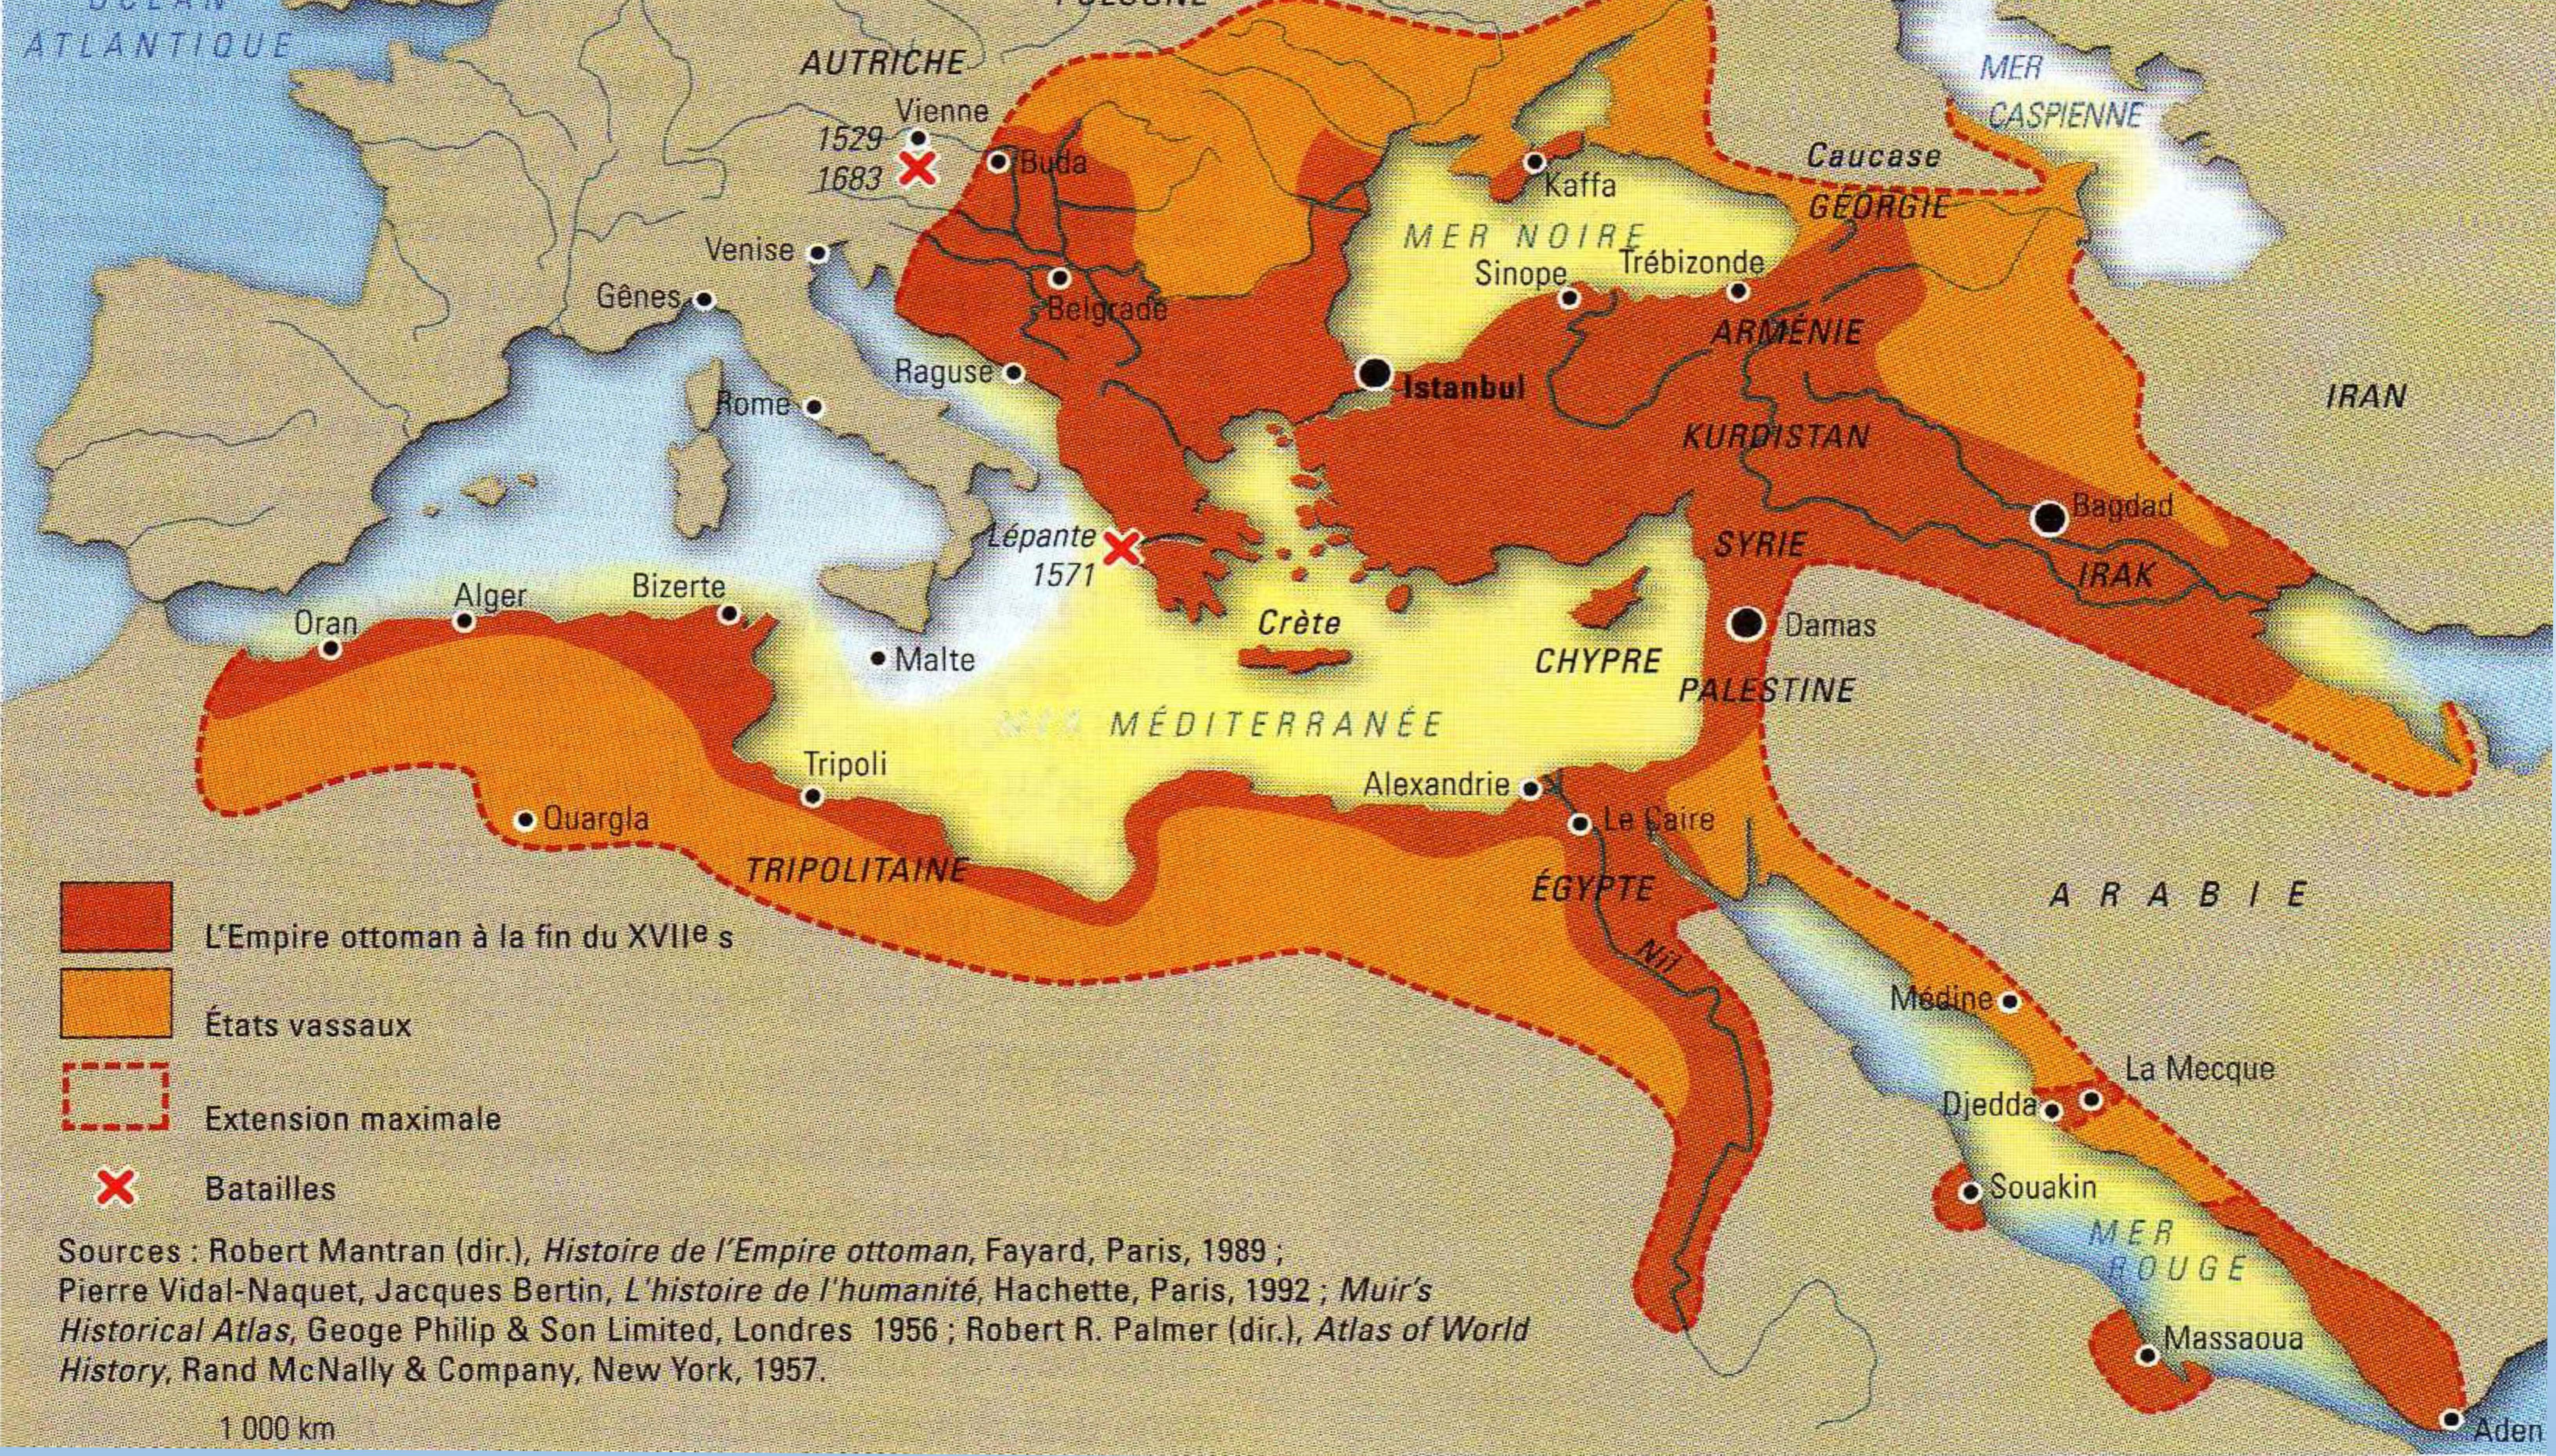
\includegraphics[width=\textwidth]{HistoireIslamMediterranee/Images/EmpireOttoman.png}
\paragraph{Fernand Braudel} s'inspire de Pirenne, mais va travailler sur l'empire des Hasbourg. Il va travailler sur la \Med dans toutes les dimensions : échange, la voir dans son unité. Il travaille avec une question : est-ce qu'il faut inventer le concept, par delà de la \Med espagnole. 

\begin{quote}
    « Dans\sn{Fernand Braudel (dir.), La Méditerranée. L’espace et l’histoire, Paris, Champs Flammarion, 1985,  p. 10} son paysage physique comme dans son paysage humain, la Méditerranée carrefour, la Méditerranée hétéroclite se présente dans nos souvenirs comme une image cohérente, comme un système où tout se mélange et se recompose dans une unité originale. Cette unité évidente, cet être profond de la Méditerranée, comment l’expliquer ? Il faudra s’y efforcer à plusieurs reprises. L’explication, ce n’est pas seulement la nature qui, à cet effet, a beaucoup œuvré ; ce n’est pas seulement l’homme, qui a tout lié ensemble obstinément ; ce sont à la fois les grâces de la nature ou ses malédictions –les unes et les autres nombreuses- et les efforts multiples des hommes, hier comme aujourd’hui. »
\end{quote}

Pour Braudel, la \Med est humaine, physique. Elle est aussi un espace d'échanges commerciaux, linguistiques. Au XIX, période la plus dense d'échanges, avec le bateau à vapeur. 


\paragraph{une \textit{rive} ou \textit{deux rives}}Après lui, les chercheurs vont s'intéresser à la définition même de l'objet : "une seule rive" : greco-romain ? ou des "deux rives", en intégrant l'héritage juif et musulman. La problématique 

\paragraph{Gardet, Berque et Massignon}{Louis Gardet, 1904-1986, philosophe chrétien des théologies comparées, islamologie. Il fonde en 1957 une revue \textit{la revue de la \Med}Il pense la \Med des deux rives, seul moyen de réduire les fractions. \textit{\Med, conception des deux rives } }. et \textit{Jacques Berque}, dépasser la rupture culturelle entre Christianisme et Islam. Islam doit fait le lien entre occident et Afrique / Asie. \textit{Louis Massignon}, Islamologue, mort en 1961, concept de l'\textit{hospitalité}. Il faut accueillir et accueillant de l'autre. Prêtre melchite en secret. Pélerinage en Côte d'Armor des 7 dormants.


\subsection{la mer partagée}

Jean Guilaine, \textit{La \Med partagée}.

La mer, qui est une mer de lien, peut être un obstacle. Avant l'Islam, des ruptures, comme en 395, la rupture entre Empire d'Orient et d'Occident. 

476 : chute de Rome.

1054 : rupture entre Eglise orient et Occident.

1204 : 4ème croisade et pillage de Constantinople.

1453 : conquête de Constantinople. 

Pirenne lui insiste sur l'irruption de l'Islam. 

D'autres insistent sur la peste du VIe siècle qui décime la \Med. 

Après les croisades, les Européens contrôlent les principales villes de la \Med mais ne connaissent pas mieux l'autre. 

\subsection{Les problématiques théologiques} 

\paragraph{Est-ce que Dieu est méditerranéen ?} Non, vue négative de la \Med. Grande mer vers le soleil couchant, mer des philistins, mer Occidentale. La fin du monde. 

\paragraph{Désert} Est-ce qu'on peut dire que le monothéisme est  méditerranéen ? Non, le monothéisme est né dans le désert. Racine sémitique, du désert, entre le Tigre et l'Euphrate.

\paragraph{Au XIIè avant JC, les phéniciens} Les maîtres de la \Med, ce sont les phéniciens qui sont sur la côte occidentale (Gaule, Carthage). La capitale de ce monde, c'est Tyr. Alphabet, art,... Est-ce une première identité mediterannéenne ? 

\paragraph{VIIème siècle : renaissance grecque archaique} \Med, plusieurs mer (Chypre, de Lybie,...). 

\paragraph{Une seule mer au temps des Romains} Avec les Romains, unité de la \Med. Paul va \textit{surfer} sur cette unité de la Mer, après la bataille d'Actium en - 31. La domination est politique mais culturellement, grecque. 

\paragraph{Une fascination de la \Med pour les Dieux} Jérusalem, Damas, 2ème capitale arabe, Rome, Constantinople + Grèce (philosophie grecque).  
\begin{quote}
   Ac 17  : Areopage 
\end{quote}
Dieu des philosophes et Dieu du désert se recontrent et ne forment plus qu'un. L'ouverture de Paul aux Nations. 

\paragraph{Conception de Jésus et la \Med.} Une ouverture à la syro-phénicienne. Jésus sort de la vision "jérusalemo-centrique".

\paragraph{Paul va s'appuyer sur l'Unité politique}
Paul. Unité religieuse de la \Med depuis 313. 3 voyages. 

\paragraph{Les fils du désert devenu des navigateurs, l'Islam} Les bébouins de l'arabie au VII vont devenir des marins. 

\paragraph{acceptation de l'Islam par la Syrie et l'Irak} 639, Syrie très vite islamisé. Pourquoi les chrétiens ont accueilli les arabes : 
\begin{itemize}
    \item peste qui a fragilisé le monde bysantin
    \item proximité culturelle
    \item un monde entre Constantinople et Perse.
    \item Nestorien
\end{itemize}

\paragraph{Apologie} de Jean Damascène 680-708. 675 : petit traité sur l'Islam. 

\paragraph{Empire Sassanide s'effondre} 
641 : l'Egypte capitule
670 : Kerouan
700 : toute l'Afrique est musulmane, plutôt paisible. 


\section{Bibliographie indicative}

\begin{itemize}
    \item     « Chrétiens et musulmans : Quel dialogue aujourd'hui ? », Cahiers de l'Atelier, tome 560, avril-juin 2019.   
    \item    ALBERA Dionigi et PENICAUD Manoël (dir.), Coexistences. Lieux saints partagés en Europe et en Méditerranée, Paris, Musée national de l’Histoire de l’Immigration – Actes sud, 2017.     
    
    \item   ALBERA Dionigi et BERTHELOT Katell (dir.) Dieu, une enquête. Judaïsme, christianisme, islam, ce qui les distingue, ce qui les rapproche, Paris, Flammarion, 2013.     
    
    \item   BERQUE Jacques, Les Arabes, Paris, Actes sud, 1999.     
    \item   BORRMANS Maurice, Prophètes du dialogue islamo-chrétien, Paris, Ed. du cerf, coll. « L’histoire à vif », 2009.     
    \item   CAHEN Claude, Islam, des origines au début de l’Empire ottoman, Paris, Hachette, coll. « Pluriel », 2011. 
    
    \item CAHEN Claude, Orient et Occident au temps des croisades, Paris, Aubier, 2010.     
    
    \item   CAILLEAUX Christophe, « Chrétiens, juifs et musulmans dans l’Espagne médiévale. La convivencia et autres mythes historiographiques », Cahiers de la Méditerranée, n°86, Juin 2013, p. 257-271.     \item   CARPENTIER Jean et LEBRUN François, Histoire de la Méditerranée, Paris, Seuil, coll. « Points Histoire », 2001.     
    \item   CAUCANAS Rémi, Relations islamo-chrétiennes en Méditerranée, entre dialogue et crispation, Presses universitaires de Rennes, 2014.   



    \item   CHEDDADI Abdesselam, Les Arabes et l'appropriation de l'histoire : émergence et premiers développements de l'historiographie musulmane jusqu'au IIe/VIIIe siècle, Paris, Actes sud, 2004.   \item DUFOURCQ Charles-Emmanuel, « La coexistence des chrétiens et des musulmans dans AlAndalus et dans le Maghrib du Xe siècle » In: Actes des congrès de la Société des historiens médiévistes de l'enseignement supérieur public, 9ᵉ congrès, Dijon, 1978, p. 209-224.  
    
    \item GAUDEUL Jean-Marie, Disputes ? Ou rencontres ?, l’islam et le christianisme au fil des siècles, Rome,   \item PISAI, coll. « Studi arabo-islamici », n°12, 1998, 2 volumes.   \item GEORGEON François, VATIN Nicolas et VEINSTEIN Gilles (dir.), Dictionnaire de l’Empire ottoman, Paris, Fayard, 2015.   \item HEYBERGER Bernard, VOGEL Jacob et ASSAN Valérie (dir.), Minorités en Méditerranée au XIXe siècle : Identités, identifications, circulations, Rennes, Presses Universitaires de Rennes, 2019.    \item HORDEN Peregrine and KINOSHITA Sharon (dir.), A Companion to Mediterranean History, Oxford, Wiley-Blackwell, 2014 (cf. Chapitre 34 “Shared Sacred Places”)    \item HOURANI Albert, Histoire des peuples arabes, Paris, Seuil, coll. « Points », 1993.   \item LEJBOWICZ Max (Eds), Les relations culturelles entre chrétiens et musulmans au Moyen Age: Quelles leçons en tirer de nos jours ?, Turnhout, Brepols, coll. « Rencontres médiévales européennes », n°5, 2005.  LOUIS Florian, Atlas historique du Moyen-Orient, Paris, Autrement, 2020.   \item MANTRAN Robert, Histoire de l’Empire ottoman, Paris, Fayard, 1989.   \item PISANI, Emmanuel,  « Le statut du ḏimmī chez al-Ġazālī », MIDÉO [En ligne], 33 | 2018, mis en ligne le 05 juillet 2018, consulté le 28 décembre 2022. URL : 
    \item REYNAERT François, La Grande Histoire du monde arabe, d'Alexandre le Grand à l'islamisme radical, Paris, Fayard, 2015.   \item REYNOLDS, Gabriel Said, The Qurʾan in Conversation with the Bible: Revised Qurʾan Translation of Ali Quli Qaraʾi annotated with Biblical Texts and Commentary by Gabriel Said Reynolds, New Haven, Yale University Press, 2018.   \item REYNOLDS, Gabriel Said, The Emergence of Islam, Minneapolis, MN Fortress Press, 2012.    \item REYNOLDS, Gabriel Said, The Qurʾān and Its Biblical Subtext, London, Routledge, 2010.   \item RODINSON Maxime, Les Arabes, Paris, PUF, coll. « Quadrige », 2002. Histoire des Arabes de 1500 à nos jours Tempus 3 ROGAN Eugene, 2016.   \item SOURDEL Dominique et Janine, 2004.   \item THOMAS History David, ROGGEMA Barbara (eds.) , Leyde  Boston, Brill, 2009 (3 volumes). , Paris, Perrin, coll. « Dictionnaire historique de l’Islam , PUF, coll. », « Quadrige », , ChristianMuslim Relations: a Bibliographical 
\end{itemize}
\chapter{Y a-t-il eu au Moyen Âge un dialogue
entre l’islam et le christianisme ?}

Rémi Brague

Je ne puis ici donner un panorama exhaustif d'une question si vaste et qui excède ma compétence. Je souhaiterais uniquement la poser de mon mieux. Il me faudra présenter le contexte d'ensemble, décrire l'espace et les orientations d'un dialogue éventuel, et souligner les contraintes qui l'ont empêché de se déployer.

\section{Le cadre historique}

\paragraph{Début de l'Islam inaccessible par le savoir}
Des débuts de l'islam, nous ne savons à peu près rien, ce qui s'appelle savoir. Les plus anciennes œuvres historiques écrites par des Musulmans ne furent composées qu'au IXe siècle, c'est-à-dire deux siècles après les événements qu'elles sont censées rapporter. Les témoignages proches ne sont pas moins orientés que les historiens musulmans, et ils sont de plus maigres et incomplets; ils nous donnent une tout autre image de "ce qui s'est vraiment passé". On a essayé d'écrire l'histoire de l'islam primitif en décidant d'ignorer systématiquement, par souci de méthode, tout ce que l'on ne peut pas dater. 
On a aussi réuni les témoignages des chroniqueurs, etc. non musulmans, de toute langue, pour les traduire en anglais et les soumettre à un examen critique.
Le plus ancien événement pour lequel on puisse indiquer une date certaine est la conquête arabe. Ce fait historique installe la scène sur laquelle la rencontre de l'islam et du christianisme a eu lieu. Notre plus ancien document est un papyrus, un reçu qui fut établi en 643 par un fonctionnaire arabe pour un paysan égyptien à qui l'on donnait quittance de l'impôt foncier versé aux conquérants. Cette guerre de conquête semble s'être déroulée comme toute autre guerre. Les Arabes n'ont été ni plus doux ni plus sanguinaires que les conquérants antérieurs, des Assyriens à Alexandre le Grand.

\paragraph{la conquête Islamique, rencontre entre Chrétiens et musulmans}
La conquête concerne le Moyen-Orient et l'Égypte, qui se trouvaient sous domination romaine - nous dirions «byzantine» -, la Perse\mn{il y avait aussi un important foyer chrétien en Perse cf \pageref{ChretienEnPerse}} qui avait sa dynastie nationale, les rives méridionales du bassin méditerranéen, et l'Espagne qui était dominée par les Wisigoths. Hormis la Perse, qui avait sa religion nationale, celle de Zoroastre, la majorité de la population - nous ne pouvons guère nous faire une idée précise de son nombre - était de religion chrétienne.
\paragraph{Une nécessaire cohabitation}Les conquérants arabes ne pouvaient ni massacrer ces gens ni les convertir en masse et d'un coup. Ils n'avaient d'ailleurs l'intention de faire aucune des deux choses. Cette cruauté aurait tué la poule aux œufs d'or. Selon une formule attribuée à 'Ali, les protégés sont «la matière des musulmans». De même, le Calife 'Umar aurait écrit à Abü 'Obeyda : \begin{quote}
    « Si nous prenions ceux qui y sont assujettis et que nous nous les partagions, que resterait-il aux musulmans qui viendront après nous ? Ils ne trouveraient, pardieu, plus personne à qui parler ni du travail de qui profiter !»
\end{quote} 

\paragraph{une asymétrie entre monde chrétien et monde musulman}
C'est ainsi que naquit une situation qui contribua de façon essentielle à déterminer la possibilité et le déroulement d'un dialogue entre religions. Elle est caractérisée par une asymétrie. Il y a dans l'espace musulman des chrétiens. Ils possèdent dans la cité islamique une place définie par le droit. En revanche, il n'y a en
terre de chrétienté, en théorie du moins, que des chrétiens et des juifs. Pour le monde islamique, les chrétiens sont donc aussi bien
<<dedans» que «dehors». Pour le monde chrétien, à l'opposé, les musulmans ne sont que «dehors». Ce n'est que de façon exceptionnelle et provisoire que des musulmans vivent en terre chrétienne.

\paragraph{quelques exceptions de musulmans en monde chrétien, mais pas d'élite}
Cela se produit là où des armées chrétiennes occupent des régions qui étaient sous domination musulmane. Ceci ne concerne guère, cependant, que les musulmans de base, paysans ou artisans ; les «intellectuels» ne restaient généralement pas sous domination chrétienne : liés au pouvoir, ils partaient avec lui. On a quelques exemples de ce genre de situation. La frontière entre l'Islam et l'Empire romain d'Orient n'est pas stable. Dans la guerre entre celui-ci et les califes, la ligne de front se déplace en Syrie, parfois assez vite. Au xe siècle, les Byzantins ont à nouveau le vent en poupe. Des villes comme Alep passent tour à tour sous domination chrétienne et musulmane. En Europe, on peut citer certaines régions d'Espagne, après la conquête, ce qu'on appelle la \textit{reconquista} du sud islamique par les royaumes chrétiens du Nord. C'est le cas de Tolède sous le règne d'Alphonse le Sage. Même cas de figure en Sicile à partir de la seconde moitié du XIe siècle, moment où les Normands prennent d'abord Messine (1061) et un peu plus tard Palerme (1072).
\paragraph{faible impact des croisades dans le monde musulman}
Les Croisades, à partir de 1096, n'ont éveillé dans le monde musulman qu'un écho faible et tardif \mn{voir Tolan}. Ainsi, le plus grand intellectuel de l'islam médiéval, et peut-être de l'islam tout court, al-Ghazalï (m. 1111), qui vivait pourtant dans la région, n'y fait nulle part allusion et semble ne pas les avoir remarquées. Ce n'est que bien plus tard, pas avant le XIXe siècle, qu'elles furent montées en épingle comme symbole de la rencontre manquée entre Orient et Occident.

%---------------------------------------------
\section{Le contexte social}

\paragraph{pas de liberté de penser}
À l'intérieur des deux domaines, le contexte des rencontres entre religions est lui aussi asymétrique. Dans chacun d'eux, une religion déterminée est la religion dominante, celle que )'on pourrait appeler, non sans anachronisme, la religion de «l'Etat». Les
gouvernants se réclament de cette religion comme à un des principes de leur légitimation. Il ne peut donc être question de permettre ce que nous appelons la «liberté de penser». En chercher l'équivalent au Moyen Âge serait parfaitement anachronique.

\paragraph{une exception : la conquête de Bagdad par les Mongols}
La seule exception, celle qui confirme la règle, le seul cas de neutralité de la puissance politique vis-à-vis des religions, est présentée par la situation qui s'était créée dans une partie du monde musulman, entre 1258 et 1290. La première date est celle de la prise de Bagdad par les Mongols. Les vainqueurs étaient bigarrés en matière de religion : il y avait parmi eux des musulmans, mais aussi des chrétiens d'obédience nestorienne, des bouddhistes, des chamanistes. Les khans n'avaient pas de religion déterminée à imposer aux vaincus, et n'en imposèrent donc aucune non plus. Une telle atmosphère permit notamment l'œuvre d'Ibn Kammü.na, qui mena entre les trois religions une comparaison qui, pour l'époque, faisait preuve d'une grande objectivité\mn{Ibn Kammuna a passé quasiment toute sa vie à Bagdad. Il y a vécu le renversement du pouvoir musulman par les troupes Mongoles de Houlagou Khan en 1258. À la suite de cela, les Mongols ont établi pour une trentaine d'années leur politique traditionnelle de tolérance religieuse, amenant avec eux une population qui comprenait chamanes, nestoriens, bouddhistes, musulmans etc. Les musulmans sont restés majoritaires dans les territoires conquis, mais cette société  n'était plus réglementée par les principes de l'islam. Il a porté un regard parfois très critique sur l'islam, mais il a aussi témoigné d'une forme d'estime pour cette religion ainsi que pour le christianisme, notamment par ses éloges de Mahomet et de Jésus. Ses écrits attestent de son attachement au judaïsme.}. Cela dura jusqu'en 1290, lorsque le Grand Khan de l'époque décida d'adopter la religion qui était déjà devenue celle de la majorité de ses nouveaux sujets, c'est-à-dire l'islam.
\paragraph{la dhimma}
Le système islamique de la \textit{dhimma}  consiste à tolérer des communautés non musulmanes, pourvu qu'elles possèdent un livre saint. Les «païens», en revanche, n'ont en principe que le choix entre la conversion ou la mort. Juifs et chrétiens sont soumis à diverses mesures explicitement destinées à leur faire comprendre, en les humiliant, l'intérêt qu'ils auraient à adopter l'islam. C'est ainsi qu'ils doivent payer un impôt spécial, se vêtir de couleurs spécifiques, renoncer à certaines montures, ne pas construire de nouvelles églises, éviter de faire sonner leurs cloches ou de chanter l'hymne trop fort, etc. Quant à ses conséquences sociales, ce système fonctionne un peu comme une nasse où l'entrée est libre et la sortie interdite. On est en droit d'adopter la religion des souverains, voire, on y est encouragé. Il est en revanche strictement défendu, en principe sous peine de mort, de la quitter en faveur d'une autre. Le christianisme médiéval appliquait d'ailleurs des règles analogues
aux Juifs, les unes dès avant l'islam, certaines inspirées de lui, comme la rouelle de couleur jaune.

\paragraph{conversion collective comme norme}
Au Moyen Age, sauf rares exceptions, la conversion vient d'en haut. Les chefs prennent des décisions en matière de religion, c'està-dire aussi en matière de politique; le peuple suit en bloc la classe dirigeante. C'est de cette façon que les tribus dites <<barbares» se laissaient baptiser comme un seul homme, une fois que leur chef s'était déclaré prêt à adopter le christianisme. Cela se passa ainsi pour Clovis, et plus tard dans l'Est et le Nord de l'Europe, jusqu'au dernier peuple à accepter le baptême, aussi tard qu'en 1386, les Lituaniens.


Des phénomènes analogues se produisirent quand par exemple l'Indonésie adopta l'islam: le rajah local se faisait musulman, son peuple suivait en masse. La conscience d'une valeur indépendante de l'individu était à l'époque plutôt une exception qu'une règle. On a un exemple d'une telle exception dans un récit sur la conquête arabe : un général musulman, passant en revue une tribu victorieuse, constata qu'elle était chrétienne. Il exigea qu'elle passât à l'islam, qui devait être l'unique religion des Arabes. Tous acceptèrent, sauf un certain Layth, qui subit le martyre. Sans cet acte de courage, nous ignorerions tout des faits.


\section{Le contexte intellectuel}

\paragraph{une langue commune, l'arabe ou des langues par communauté}
Entre la situation de la chrétienté et celle du monde islamique, on observe une différence capitale. Dans le premier cas, chaque communauté religieuse possède sa langue de culture, qui est selon les régions le grec ou le latin. Dans le second, même si les communautés chrétiennes gardent longtemps une langue liturgique bien à elles, comme le copte ou le syriaque, il se met en place assez rapidement une langue de culture commune, qui est l'arabe. Celui-ci est langue de l'administration depuis 750. Quant à la possibilité d'un dialogue entre religions, le fait entraîne des conséquences positives et négatives. Dans le monde islamique, la présence d'une langue commune permet, c'est l'aspect positif, une intercommunication très facile. En revanche, les non-musulmans peuvent être compris sans trop de difficulté de leurs souverains musulmans et doivent donc prendre leurs précautions. 1.;usage d'un alphabet différent ne suffit que jusqu'à un certain point. Une attaque frontale contre la religion dominante est à peu près impensable.
On voit bien les conséquences quand on compare la situation des Juifs en chrétienté et en terre d'islam. En terre chrétienne, les Juifs emploient, dans la vie quotidienne, la même langue que les chrétiens, à savoir le vernaculaire local. Mais si l'on se place au niveau du savoir religieux et, socialement, dans le milieu des clercs de chaque religion, les conditions du dialogue intérieur avec le judaïsme deviennent analogues à celles qui déterminent le dialogue extérieur entre Islam et Chrétienté. Les rabbins et les clercs chrétiens n'écrivent pas la même langue, mais, respectivement, l'hébreu et le latin ou le grec. Les oulémas écrivent l'arabe, alors que leurs adversaires chrétiens s'expriment en grec ou en latin. D'où un dialogue de sourds. Par ailleurs, écrire sa propre langue offre une protection qui permet aux hétérodoxes de dire ce qu'ils ont sur le cœur. Les Juifs peuvent par exemple mettre en circulation les Toledot Yeshu, qui offrent une version anti-chrétienne de l'histoire du Christ. Les choses ne s'envenimèrent que lorsque des transfuges mirent en garde leurs nouveaux coreligionnaires contre le contenu des livres de la religion de leurs pères.

\paragraph{bonne connaissance de l'Islam par Byzance}
À l'intérieur même de la chrétienté, il y a des différences entre
l'Orient et l'Occident. Byzance connaît l'islam relativement bien, et relativement tôt, avant même que la dogmatique islamique ne se cristallise. Ainsi, la polémique de saint Jean Damascène, peu avant le milieu du vrne siècle, nous présente un état des questions disputées dans l'islam de l'époque7. Le Coran est traduit en grec dès le 1xe siècle, d'ailleurs pour pouvoir être réfuté plus efficacement.

En revanche, les européens connaissent l'islam assez mal. Pour eux, les musulmans sont simplement des païens. Cette façon de voir a aussi des raisons concrètes. Le premier contact avec des musulmans ouvrit en effet un second front au sud, alors que l'Europe était
déjà assiégée au nord par les Normands. Comme l'Europe croyait elle-même représenter la chrétienté, elle considéra ses ennemis comme étant, globalement, des païens. Dans une situation d'urgence, des nuances plus subtiles n'avaient guère leur place. D'où la caricature que l'on trouve encore dans la \textit{Chanson de Roland}: le «sarrasin» est un idolâtre, qui adore trois divinités, parmi lesquelles :figure aussi Muhammad.

\paragraph{XIIè : Pierre le Vénérable}
Ce n'est qu'à partir du xiie siècle que le portrait-charge naïf le céda à une vision plus nuancée de l'adversaire. Pierre le Vénérable, abbé de Cluny (m. 1156) fit traduire en latin le Coran ainsi que d'autres œuvres donnant une idée plus juste et plus précise de l'iJlam. Ce dossier produit par des érudits réunis dans la vallée de l'Ebre forme ce que l'on appelle la \textit{collectio toletana}. Mais le manuscrit qui le contient n'a à peu près pas circulé, et son contenu ne fut imprimé qu'au XVIe siècle.
\paragraph{XIII : Roger Bacon  et Lulle}
Au xiiie siècle, le besoin se fit sentir d'une meilleure connaissance de l'islam. Le franciscain Roger Bacon (m. 1292) fit figurer parmi l'ambitieux programme de réformes qu'il soumit au pape la fondation d'écoles de langues qui devraient enseigner entre autres l'arabe. Raymond Martin, un dominicain catalan, se familiarisa suffisamment avec l'arabe et l'hébreu pour pouvoir écrire son célèbre \textit{Pugio fidei adversus mauros et judaeos} (1278), dont le titre indique bien l'intention polémique. Raymond Lulle (1233-1315), catalan originaire de Majorque qui avait été reconquise peu avant sa naissance, se donna la peine d'apprendre l'arabe pour composer en cette langue des présentations du christianisme à l'usage des arabophones, lesquelles semblent malheureusement avoir été toutes perdues.



\section{Le contexte affectif}

La connaissance de chacune des deux religions par l'autre est souvent assez mauvaise. Mais ce n'est pas pour les mêmes raisons. Il importe de se rendre compte des obstacles. Ils sont symétriques, mais inversés. Pour le dire en une formule évidemment sommaire : \textbf{les chrétiens savent qu'ils ne connaissent pas l'islam; les musulmans croient qu'ils connaissent le christianisme.}

\paragraph{Difficulté à penser l'Islam pour le Christianisme}
Pour le christianisme, l'islam est quelque chose qui n'aurait pas dû exister. L'islam est un imprévu, quelque chose de nouveau et d'inattendu, et donc de paradoxal. Les Chrétiens en tant que tels savent, ou croient savoir, ce que c'est que le judaïsme et ce que c'est que le paganisme. Or, les musulmans ne se laissent pas classer dans une catégorie préexistante: l'islam n'est pas païen- en tout cas il est monothéiste ; il n'est pas non plus juif; il est encore moins chrétien. C'est ce qui expïque une surprise qu'on n'a pas de mal à sentir chez les Pères de l'Eglise qui ont eu à faire avec l'islam. Ainsi Jean Damascène, déjà cité, considère l'islam comme une hérésie chrétienne.

\paragraph{Le Christianisme est réduit/ordonné dans l'Islam}
Rien de tel pour l'islam. Pour lui, le christianisme est quelque chose de bien connu, une vieille histoire. Le Coran contient des renseignements sur les chrétiens : ils adorent à côté du Dieu unique d'autres entités, comme Jésus et sa mère. Le christianisme est quelque chose de dépassé. Les chrétiens se sont refusés à reconnaître le prophète définitif qui devait parachever leur religion. Ils ont manqué le coche. De plus, ceux des chrétiens concrets qui sont présents sous domination musulmane, divisés en sectes qui s'anathématisent réciproquement, et maintenus dans une humiliation commune, ne semblent pas avoir grand-chose d'intéressant à enseigner.

\paragraph{Asymétrie psychologique}
De telles façons de voir ont des conséquences quant aux affects fondamentaux de chaque religion envers les autres. Nous n'éprouvons pas face à l'inconnu les mêmes affects qu'envers ce qui nous est familier. Quand les choses se passent bien entre les deux religions, l'islam est aux yeux des chrétiens un objet de curiosité qui peut fasciner, une sorte d'\textit{enfant terrible} que l'on regarde avec une tendresse indulgente ; quand au contraire les choses vont mal, il devient un objet de haine et de crainte.

\paragraph{pas de curiosité de l'Islam pour le Christianisme}
Réciproquement, quand les choses vont bien, le christianisme est pour l'islam un objet de sympathie, cette sympathie condescendante que l'on a envers un vieil oncle un peu gâteux et qui rabâche toujours les mêmes histoires. Mais il n'est en aucun cas un objet de curiosité. La curiosité envers l'autre est d'ailleurs une attitude typiquement européenne, rare hors d'Europe, et exceptionnelle en Islam. Quand les choses vont mal, l'islam éprouve envers le christianisme beaucoup moins de la haine que du mépris.


En dernière instance, cette attitude dépend directement de la place que les deux religions occupent dans l'histoire. Très platement: l'une vient avant l'autre. Mais cet ordre n'est pas que chronologique. Il a été l'objet d'une réflexion. Très tôt, à vrai dire dès qu'il s'est constitué comme une dogmatique indépendante, l'islam s'est compris comme un post-christianisme: les plus anciens textes de style coranique que l'on puisse dater sont les inscriptions du Dôme du Rocher, à Jérusalem, qui attaquent la Trinité. L'islam se voit comme la dernière religion, la religion définitive, celle qui relève le judaïsme comme le christianisme, au sens de la « relève » telle que le concevait Hegel (\textit{Aufhebung}), laquelle tout à la fois abolit et assume ce qui la précède et la prépare.

\section{Esquisse de la littérature apologétique}

Je ne puis ici risquer qu'un coup d'œil rapide et pour l'essentiel de seconde main sur la littérature polémique et apologétique
\paragraph{littérature apologétique : constitutive de l'Islam}
Elle s'adresse avant tout à ceux qui partagent la religion de leur auteur. Elle est à usage interne. Il ne s'agit pas de convaincre l'autre de se convertir en montrant les beautés de sa propre religion. Il s'agit bien plutôt de décourager ses coreligionnaires d'abandonner leur foi en faveur d'une autre religion, dont on devra donc faire ressortir les absurdités. Cela n'encourage guère l'objectivité, encore moins l'effort pour comprendre avec sympathie la position de l'autre.
La situation n'est pas la même pour le christianisme et pour l'islam. Le christianisme a dû se séparer du judaïsme, du paganisme,
de la gnose, de ses propres hérésies; en revanche, il n'a bien évidemment pas eu à se définir en se distinguant de l'islam qui n'existait pas encore. Alors que celui-ci entre en scène, la dogmatique chrétienne est en place depuis des siècles. En revanche, l'islam a dû se définir contre un christianisme qui était déjà là. La polémique contre le christianisme (et déjà contre le judaïsme) n'est pas pour l'islam secondaire, elle est constitutive. Le premier livre de polémique anti-chrétienne de l'islam n'est autre que son tout premier livre en général, c'est le Coran.

\paragraph{Risque du synchrétisme chez les musulmans}
Plus tard, la polémique fut rendue nécessaire non pas malgré les conversions à l'islam, mais, paradoxalement, par le mouvement même de ces conversions. Se faire musulman est très facile. Il suffit de prononcer devant témoins une courte formule de confession de foi (\textit{shahiida}). Le catéchisme auquel on adhère est bref et assez plausible \mn{Eglise vs Secte}. Et les musulmans n'ont pas l'habitude de mettre à l'épreuve la conviction du néophyte. Une telle attitude ne manque pas d'avantages évidents. Mais elle fomente un danger, celui du syncrétisme chez des gens qui ne se sont convertis que pour la forme ou sans vraiment savoir à quoi ils s'engageaient, et qui cherchent à introduire dans l'islam le plus possible du contenu de leur religion précédente. L'islam craint donc de se dissoudre dans une vague religiosité composite. La polémique sert à immuniser les musulmans contre le christianisme.
\paragraph{contre les affirmations christologiques, la Trinité, la falsification de la Bible}
Les contenus de cette polémique sont toujours les mêmes et roulent sur les grands thèmes de la christologie et de la Trinité, de la Bible: a-t-elle été corrompue par ses porteurs ou gardée intacte? Muhammad y a-t-il été prédit? De temps en temps, elle prend une allure sociale, et les musulmans se plaignent de la trop grande influence des chrétiens, médecins par exemple, dans la société. Le thème d'une corruption historique du christianisme mise au débit de saint Paul n'apparaît qu'au xme siècle avec 'Abd al-Jabbar, qui a peut-être utilisé des textes judéo-chrétiens.

\paragraph{Une religion par la force, quel signe du Prophète}
Les arguments sont eux aussi récurrents. Ainsi ceux des chrétiens: comment une religion est-elle venue au pouvoir, pacifi-
quement, ou par la force des armes? À quoi reconnaît-on l'authenticité de la mission d'un prophète ? Est-elle corroborée par des miracles? Le prophète se distingue-t-il par un mode de vie particulièrement édifiant? Ces questions d'allure purement historique sont biaisées: il s'agit de faire ressortir le caractère militaire de l'expansion de l'islam, l'absence de miracles chez Muhammad, sa vie sexuelle agitée. Dans ce genre de littérature, tous les arguments sont bons, pourvu qu'ils frappent l'adversaire. On comprend que la lecture de ces textes ne donne pas une idée très positive de la nature humaine...

\section{Dialogues ?}

\paragraph{Caractère fictif des vrais dialogues}
En fait de dialogues, nous possédons avant tout des œuvres littéraires qui se présentent comme si elles reproduisaient des discussions réelles entre les représentants de diverses religions. Mais il s'agit de fictions. C'est le cas du \textit{Dialogue entre un philosophe, un juif et un chrétien} de Pierre Abélard (vers 1140), dans lequel le philosophe est un musulman, peu orthodoxe il est vrai. C'est aussi le cas du \textit{De pace fidei} écrit par le cardinal Nicolas de Cuse au lendemain de la prise de Constantinople (1453), ou encore du \textit{Colloquium Heptaplomeres} que le juriste français Jean Bodin écrivit probablement vers 1593.
De véritables dialogues entre des personnages réels où chacun exprimerait dans son vocabulaire à lui ses convictions authentiques, restent une exception. On cite partout une disputation de ce genre, censée avoir eu lieu à Bagdad. Les représentants de chaque opinion, même les moins admises, y auraient pu s'exprimer librement, tous se seraient mis d'accord pour s'abstenir d'argumenter sur la base d'un texte scripturaire, etc.14 Il n'en faut pas moins pour enflammer l'imagination« multiculti » de nos belles âmes. L'anecdote provient en fait d'un orthodoxe des plus étroits, qui ne la rapporte que pour
dire son scandale. N'aurait-il pas, sinon tout inventé, du moins considérablement forcé le trait?

\paragraph{Caractère polémique et institutionnel des dialogues}
La plupart du temps, le contexte des dialogues est polémique. On peut signaler la \textit{disputatio} tenue le 30 mai 1254 à Karakorum, en présence du khan des Mongols Mongke, à laquelle prirent part le franciscain flamand Guillaume de Ruysbroek (Rubruquis), envoyé de Louis IX et du pape, des chrétiens nestoriens, des bouddhistes et des musulmans. Mais notre seule source est le franciscain lui-même, qui s'est sans doute, et bien naturellement, donné le beau rôle.
Entre juifs et chrétiens, les disputations (\textit{wikkuah}) sont institutionnalisées. Les juifs sont contraints à disputer, la plupart du temps pour répondre aux accusations d'un de leurs coreligionnaires passé au christianisme. Cela ne se fait pas sans une certaine équité. Ainsi, le roi d'Aragon, pourtant chrétien, déclara vainqueur le rabbin de Gérone Nahmanide dans la polémique qui, à Barcelone, en 1263, l'opposait au converti Pablo Cristiani, et lui décerna même une récompense en argent. Reste que l'atmosphère de tels débats est dans l'ensemble désagréable, la pression sociale s'exerçant en sens unique. Elle ira d'ailleurs en s'accentuant jusqu'à l'expulsion finale de 1492.

\paragraph{Quelques exceptions}
Entre chrétiens et musulmans, les disputes publiques n'ont pas
de caractère institutionnel et sont plus rares. Les légendes ne manquent pas, par exemple à propos de saint François. Raymond Lulle
:fit une tentative de ce genre à Bougie, et y fut lapidé. On a peut-être un cas, mais notre seule source à ce sujet est un poème espagnol,\textit{ La Disputa que fue ficha en la çibdad de Feç delante del Rey e de sus sabios}, supposé écrit à Nicosie (Chypre) en 1469, et rapportant une dispute tenue à Fez en 139417. Elle se serait terminée par la conversion du principal docteur de la Loi musulmane (\textit{faqïh}) de Fez. On peut y voir, pour dire le moins, une certaine stylisation ... Il est en tout cas
intéressant que la dispute se serait déroulée à propos d'un livre sur la Trinité et l'Incarnation, écrit en arabe, intitulé \textit{Condus} (peut-être \textit{Quddüs}, « très saint»), et œuvre de Raymond Lulle. Par ailleurs, le climat global de tolérance semble correspondre assez bien à la réalité de l'époque.


\section{Conclusion: « prêcher des convertis »}

Ainsi, au Moyen Âge, les véritables dialogues entre islam et christianisme sont des plus rares, et, si l'on entend par-là des dialogues tels que ceux qui nous semblent souhaitables, simplement inexistants. La littérature polémique s'adresse à des gens déjà convaincus. Le dialogue est plutôt un genre littéraire qu'une réalité. Les essais de traiter l'autre avec équité, et, déjà, de bien le comprendre, restent une exception. On a certes de droit de rêver à de tels dialogues entre religions pour l'avenir. Mais rien ne nous autorise à projeter ce rêve dans le passé médiéval. Notre entreprise est peutêtre noble, mais elle ne doit pas sa noblesse à de quelconques ancêtres.


\section{Discussion}
\newline M. Alain BESANÇON. - J'ai relevé des points qui peuvent introduire des discussions plus vastes. La conquête, par le bas, de façon pacifique, de la société par les chrétiens ne va durer que jusqu'à Constantin. Ensuite la conversion s'est souvent opérée par le sommet. Celle de l'Allemagne, du Nord en particulier, s'est faite par le fer et par le feu - d'une façon assez musulmane - et la conversion de la Scandinavie, de la Pologne, de la Russie, de la Hongrie, dans toute l'Europe de l'Est et du Nord s'est faite par les princes. Ce sont les princes qui baptisaient leurs sujets, les plongeaient dans les rivières et les lacs pour recevoir le sacrement. Au sujet des conquêtes de l'Islam, il faut se souvenir que les Arabes n'étaient pas tellement nombreux. J'ai l'impression qu'il y a eu un mouvement de boule de neige. En un siècle, ils sont allés des frontières de la Chine à Poitiers. Cela a été permis par une conversion simultanée de masses chrétiennes à l'islam et, en particulier, de toutes les églises travaillées par l'hérésie (nestoriens, monophysites, donatistes, ariens d'Espagne). Pour l'Espagne, il est je crois reconnu que la conquête de l'Islam par les Arabes est facilitée par un retour de flamme de l'arianisme. Les chrétiens sont devenus rapidement musulmans. Ils ont ouvert les portes aux petites troupes conquérantes. Les juifs, que l'on tracassait depuis des siècles, ont aussi ouvert les portes aux conquérants musulmans en espérant qu'ils les laisseraient davantage en paix.
Vous avez dit que toutes les œuvres de Raymond Lulle ont disparu. Il existe pourtant son Livre du gentil est des trois sages où il imagine un dialogue entre les trois religions.
\newline M. Rémi BRAGUE. - Ce sont les œuvres arabes qui ont disparu. Sinon, il reste beaucoup d'œuvres de Raymond Lulle, qui est un auteur extraordinairement prolifique.
\newline M. BESANÇON. - Il me semble qu'il n'a rien compris à l'islam. Il n'a fait que projeter son christianisme sur l'islam.
La protection de la dhimma a touché les juifs, les chrétiens, les zoroastriens et ce que l'on a appelé les sabéens. Elle n'a pas touché les hindouistes. C'est pour cette raison que la conquête de l'Inde par l'Islam a été d'une telle cruauté: les hindouistes étaient considérés comme des kafirs, des infidèles. Ils avaient donc le choix entre la conversion à l'islam, qui s'est souvent produite, et la mort ou l'esclavage.
Vous avez touché à une équivoque dont nous allons parler certainement dans la journée: les musulmans sont-ils des païens ou non?
Intervenant non identifié. - Doit-on écrire Islam avec une minuscule ou avec une majuscule ?
\newline M. BRAGUE. -  C'est une convention adoptée par certains savants occidentaux, et français évidemment puisque nous avons la chance d'avoir une langue où il y a des majuscules et des minuscules. C'est un moyen commode de trouver pour l'Islam l'équivalent de cette distinction qui existe dans les langues européennes entre christianisme - la religion - et chrétienté, Christendom et Christianit:y, Christantum et Christenheit. C'est facile dans les langues de l'Europe. En français, il n'y a qu'un mot.
L'islam, avec une minuscule, est le nom commun qui désigne l'attitude d'abandon de soi sans réserve dans les mains de Dieu: il s'agit de la religion musulmane. L'Islam, avec une majuscule, est un nom propre qui désigne une réalité historique et géographique: il s'agit du monde musulman, de la civilisation musulmane.
Lorsque j'ai esquissé cette symétrie entre christianisme et islam primitif, je voulais expliquer une seule chose, à savoir la constitution d'une chrétienté - l'Empire romain - et la constitution de l'Islam - l'Empire arabe. Pour la suite des opérations, effectivement, il y a aussi une symétrie. Le christianisme, devenu chrétienté, s'est étendu par des moyens aussi bien militaires que pacifiques. Des missionnaires étaient en même temps des soldats, parfois dans la même personne, comme les chevaliers Teutoniques et les chevaliers PorteGlaive. En Islam, réciproquement, il y a eu aussi bien une poursuite de l'expansion militaire - vous avez fait allusion à ce sympathique personnage, Mahmüd de Ghazni, que l'on n'a toujours pas oublié aux Indes-, mais il y a eu aussi une expansion pacifique qui se faisait, de la même façon, par conversion des princes. Ainsi, à une époque plus proche de nous, l'Indonésie est devenue musulmane. Les radjahs se sont fait musulmans, comme Clovis s'est fait baptiser avec tout son peuple.
Concernant les conversions de masse chrétiennes, je n'en sais rien. l;historio­
graphie est extrêmement dangereuse à utiliser, en particulier lorsqu'elle raconte que les populations locales ont accueilli les conquérants arabes comme des libérateurs. C'est un topos historiographique que l'on retrouve constamment et à notre époque aussi. Si l'on étudie les témoignages contemporains - un Américain, Robert Hoyland, les a récemment recueillis dans un gros volume-, les témoignages du vu. siècle, les chroniqueurs arméniens, géorgiens, grecs, de langue syriaque de l'époque, on s'aperçoit que c'est une conquête comme les autres, ni plus ni moins sanguinaires que la conquête lambda, celles d'Alexandre le Grand ou des Romains par exemple18. Après, on voit apparaître ce genre littéraire, sous la plume
même de chrétiens expliquant que, lorsque les Arabes sont arrivés, on les a presque accueillis avec des fleurs. C'est intéressant, mais c'est un fusil à deux coups.
Qui écrivait ces chroniques ? Des gens qui vivaient sous le système de la dhimma, des gens sous la protection musulmane et qui devaient négocier cette protection, en particulier, sur le fond de l'attitude qu'ils avaient eue envers les conquérants. En d'autres termes, celui qui avait ouvert sa porte aux conquérants arabes avait de bonnes conditions. Mais, pour celui qui avait combattu et avait dû se rendre, les conditions étaient plus dures. Les historiens chrétiens avaient donc tout intérêt à essayer de faire croire aux souverains musulmans que cela s'était passé dans la paix, l'harmonie, la bonne humeur et que l'on avait offert le vin chaud du soldat aux conquérants arabes. Alors attention aux historiens !
\newline M. BESANÇON. - Ce que vous dites m'intéresse beaucoup. Si je rassemble de vieux souvenirs: Ne peut-on pas dire qu'il y a eu un allègement fiscal temporaire parce que les impôts byzantins ont cessé d'être levés et que les Arabes ont mis en circulation les trésors byzantins? Ensuite la fiscalité arabe, discriminatoire envers les juifs et les chrétiens, est intervenue puissamment pour convertir ceux-ci? Si j'ai bien compris, on les a essentiellement convertis par les impôts.
\newline M. BRAGUE. -  Oui. C'est très humain.
\newline M. BESANÇON. - Élisabeth a converti les catholiques d'Angleterre par le même moyen. La discrimination :fiscale est un moyen efficace.
\newline M. BRAGUE. - Les gens de Constantinople embêtaient les nestoriens et les jacobites. Il y a eu donc un moment pendant lequel l'arrivée des conquérants arabes a été ressentie comme un soulagement par les minorités religieuses contre lesquelles l'État byzantin était pesant. Cela n'a peut-être pas duré très longtemps, mais ce sentiment a existé. Les membres de ces minorités n'avaient plus à penser ce que le basileus voulait qu'ils pensent. Les Arabes étaient religieusement neutres. On ne savait pas trop quelle religion ils professaient - peut-être ne le savaient-ils pas très bien eux-mêmes.
\newline M. BESANÇON. - Jean Damascène, un des premiers témoins, dans son premier traité décrit l'islam comme «l'hérésie numéro cent». Il semble la considérer comme un nouveau chapitre des hérésies chrétiennes. Dans le second traité, il en parle avec condescendance comme des chrétiens d'aujourd'hui parleraient des mormons, c'est-à-dire comme de gens tout à fait éloignés du christianisme.
Je passe maintenant la parole au Père Emilio Platti, qui est dominicain. Il est aussi professeur à l'Université catholique de Louvain, à l'Institut catholique de Paris et il est membre de l'Institut dominicain des Études orientales du Caire.


\section{Texte}

\subsection{Disputa }

\begin{quote}
    Enla ciudat de Fes que es tierra de Moros fue fecha disputa delante de el rey et de rodos sus suabros alfa quis et letrados en el mode segniente  
\end{quote}

\begin{quote}
Et el dicho moro Abraym magaluf se fue en Portogal e se figo christiano e morio en la servicio de dios el qual plega dela querer per donar e anos otros asy mesmo.
\end{quote}
%\chapter{Des pratiques religieuses revisités}
\mn{PLAN 4. ISTR. C. Valasik
}

\section{des modèles revisités}
 (D. HERVIEU-LEGER)
\subsection{La figure du converti}
\mn{Pélerin et le converti, Hervieu Leger}
Avant ma vie n'avait pas trop de sens. Disqualification de la vie précédente : 
\begin{quote}
    il s’adonne jusqu’à 30 ans «aux vanités du monde, avec un grand et vain désire d’y gagner de l’honneur».Récit du pélerin
\end{quote}
\paragraph{révélation}
On aime à y revenir et le raconter. Cette révélation donne un sens à la vie.

\paragraph{ma vie a changé} je peux vivre des épisodes difficiles mais je me sens porté. Mais je suis porté non seulement par la personne que j'ai rencontré mais aussi la communauté.

\paragraph{Radicalisation} Ils vont devenir très normatifs. \textit{je vais faire ce qui est la norme}. 
\begin{Ex}
    je vais faire les 5 prières de l'Islam
\end{Ex}
Je vis de cette radicalisation car comme je suis dans la joie et donc, si je m'éloigne de la pratique, je risque de quitter cette joie. \textit{visibilité de cette pratique}.

\begin{Ex}
    On assiste actuellement à une radicalisation des jeunes juifs par rapport à la Casheroute.
\end{Ex}

\begin{Ex}
    Conversion dans les professions de santé : comprendre pourquoi cela va mal et permet de gérer l'impuissance. 
\end{Ex}

\paragraph{Je veux témoigner de ma vie} Je vais faire du prosélytisme : \textit{volonté de témoigner}. 

\paragraph{intégrer le converti dans une Eglise} Des processus pour intégrer la personne qui bouge. 

Témoignage et expérience du choix individuel
\paragraph{3 modèles de converti}
\begin{itemize}
    \item Ceux qui n'avaient aucune religion
    \item Ceux qui avaient une religion (bcp catholicisme vs pentecotisme ou Islam)
    \item converti de l'intérieur.
\end{itemize}

\paragraph{Aux USA} la foi qu'on peut avoir une seconde chance. Cette figure du converti est très forte. En France, pas de seconde chance valorisée.


\paragraph{Avec l'individualisme} on est dans des logiques de conversion intérieure. Du fait de l'importance de la liberté.

\paragraph{Changement de paradigme} sur le religieux. \mn{Coming Out : très drole}


\begin{Synthesis}
    Une approche de converti très moderne du fait de l'individualisme.
    Les convertis vont prendre certains aspects de la religion plus que d'autres.
    
\end{Synthesis}
\mn{29/11/22}
\paragraph{on va étendre ce concept à d'autres domaines} \textit{conversion politique}. \textit{Aborder la conversion écologique}

\subsection{La figure du pèlerin}

\begin{Def}[pélerinage]
    On ne vit que par et pour sa religion pendant un moment. On va vivre des moments intenses.
\end{Def}

\paragraph{mobilité géographique} temps extraordinaire. 

Mobilité et sociabilité extra-ordinaires

\paragraph{figure très moderne} car décision

\paragraph{cela coupe du quotidien} On va se centrer sur ce temps

\paragraph{Rencontres} Proximité émotionnelle et affective très forte des personnes qu'on rencontre. 

\textit{autres espaces, autres temps, autres personnes}

\paragraph{A des moments particuliers de la vie} réflexion, chomage, retraite, maladie (Lourdes).

\paragraph{fatigue} les JMJ sont considérés comme des temps de pélerinage, et les jeunes aiment. \mn{Taizé pareil.}


\paragraph{Attrait des jeunes} Les modalités d'engagement des jeunes : on donne tout à fond. Avec une difficulté, qui est le \textit{retour}.


\paragraph{Mais pas de suite sur du temps long dans la paroisse} Recherche d'une pratique valorisant la louange, pas dans la paroisse (Emmanuel,...).


\paragraph{Ce qui est important, c'est le chemin, pas le but}

\paragraph{Renforce l'appartenance religieuse} Un \textit{nous} qui va se matérialiser par d'autres pélerinages, d'autant plus 




\paragraph{Ne pas opposer pelerin et converti}




\paragraph{De la religiosité populaire} Ce n'est pas la même population qui va à chaque pélerinage. Impuissance des institutions qui essayent d'orienter mais qui lui échappent.
On peut voir aussi des pratiques perpétuées (flagellation,...). 

\mn{Elisabeth Claverie : anthropologue des pélerinage, décrit les pélerinages : qu'est ce qui se passe pour eux. Pourquoi ils vont à Mejugorge ? Enjeux commerciaux, politiques}


\subsection{les fidèles habituels}
Continuent d'être en lien avec l'institution, ne l'ont pas quitté.
Ceux qui quittent l'Eglise cathologique sont par définition difficiles à identifier, s'ils partent de façon silencieuse. 
Les fidèles habituels continuent à avoir un lien avec l'institution mais ils s'autorisent des accommodements.

\section{les formes modernes de la religiosité }

Il s'agit ici de revoir les différents points déjà vus de façon différente.

\begin{Def}[Religiosité]
    Cela relève du religieux mais pas toujours de façon très bien définie
\end{Def}


  \paragraph{Individualisation du croire} : quelque soit mon modèle, je suis travaillé par la modernité et l'individualisation. Je crois en fonction de l'héritage reçu et du cadre (Gabon, France) mais je prends que ce qui fait sens à un moment dans ma vie. Les gens n'ont pas forcément conscience.

    \begin{itemize}
        \item  on va mettre de l'exigence mais on va faire valider notre pratique par des laics et non des religieux. 
    \end{itemize}
    
      \paragraph{Importance de l’émotion} : le protestantisme émotionnel, les charismatiques catholiques
    \begin{itemize}
        \item Face à la suprématie de la raison, un certain nombre de courants s'opposent à cette suprématie de la raison \mn{Mai 68 était aussi anti raison et pourtant les religions sont souvent anti 68}
        \item on pense que la raison éloigne de la vérité (croyance) et que finalement, à trop vouloir comprendre, on s'éloigne de ce qu'est la vie.  Tous ceux qui ont la connaissance, auraient une position du surplomb, méconnaitraient la \textit{vraie vie} qui elle serait non raison.
        \item Le prêtre, le patron, Policier, président, Père, professeur : les figures d'autorité vont être remis en cause dans les années 60. 
        \item valoriser les sentiments au bénéfice de la raison. Ce qui serait juste dans ma vie, c'est ce que je ressens. \mn{Cela s'auto justifie : \textit{je ne sens pas le prof}, \textit{je ne le sens pas} et donc je ne le fais pas. Ce n'est pas argumenté.} 
        \item si vous critiquez ce que je ressens, vous m'attaquez. Quand on est sur des discussions sur des argumentaires et la raison, on ne se sent pas attaqué et donc le dialogue devient possible.  D'où la communication non violente : \textit{je comprends ton ressenti}. Attention, cela ne veut pas dire que le sentiment serait faux. 
        \item dans les mouvements religieux, important en particulier pour les jeunes.  Des discours de prêtres à partir du témoignage et pas des figures de conviction par la connaissance. \textit{des liturgies fortes qui engagent le corps}. 
        \item Les charismatiques catholiques et évangéliques vont valoriser l'émotion. Certains Groupes évangéliques : \mn{Sebastien Fath}
        \begin{Ex}[Pentecotisme - Immédiaté]
            Je dois changer de travail. je tire une phrase de la bible au hasard.
            Dire ce que la phrase me fait ressentir. 
            Si j'ai le Lévitique, j'ai le droit de retirer. Comment les personnes questionnent la phrase et se l'approprient. \textit{Comment le texte religieux nous aide au quotidien}. Avec le Groupe qui travaille avec vous.
        \end{Ex}
         Il faut que la religion soit efficace. 
         \item \textsc{Ces personnes ont besoin d'un cadre normatif très clair} : s'habiller, s'alimenter. 
         \begin{Ex}[Pentecotisme]
             On va nettoyer sa vaisselle avant de sortir de chez soi. 
         \end{Ex}
         Et finalement, on va rationaliser sa vie par ce cadre. Je le fais \textit{parce que je le sens}. Dans notre société, il y a tellement de possibilités de choix que 
    \end{itemize}
     \paragraph{La guérison}
 Demande que la religion nous guérisse. dés-envoûtement. La religion est le lieu du bien mais aussi le seul lieu où on parle du mal (exorcisme). Cela peut être actionné par des flux migratoires. C'était en sommeil mais cela se réveille.

 Les religions sont un soutien auprès des personnes malades. Comme la maladie découpe la personne (\textit{patient touché par tel maladie}). Ce que propose les confessions religieuses, c'est de proposer un parcours au malade : \textit{tu es certes malade mais tu n'es pas que cette maladie}. 

 Il peut y avoir une injonction moderne de trouver du sens, alors qu'il n'y en a pas forcément. Les personnes en situation de maladie se tournent vers la religion, avec une acceptation de la maladie par les religions (cf S Jean Paul II).

 Différentes demandes : 
 \begin{itemize}
     \item guérison
     \item moins souffrir
     \item homéopathie, ostéopathe : aide à reconstruire une globalité. les gens qui sont intéressés par ce type de pratique vont être attirés par les groupes spirituels.
 \end{itemize}
     
     \paragraph{La conversion}
Valorisation, surtout dans le protestantisme évangélique, avec l'impératif de témoigner de sa conversion. Je vais convertir sur mon témoignage. 
     
 \mn{voir le film sur Bourdieu : \textit{la sociologie est un sport de contrat}}


\paragraph{devoir} Pour les travaux, s'appuyer sur des textes ou des livres. Identifier la question de départ. Et du coup, on peut savoir si on a besoin de lire ou pas. Quels sont les moyens de répondre. 
%\chapter{Comment penser le religieux et la religion}

\mn{PLAN 5. ISTR. C. Valasik Les approches fonctionnaliste et substantiviste.}


 \section{Genese du Religieux}

 \subsection{Emile Durkheim (1858-1917) }
 
 Différenciation entre le profane et le sacré  Le savoir religieux est de nature symbolique. Il exprime des réalités sociales indicibles dans une langue particulière.  La religion fournit un sens du monde, elle structure le sens du non-sens.  

 \subsection{Max Weber (1864-1920) }

 Le développement des villes, l’urbanisation et la division du travail engendrent une demande du sens.  Cette attente de sens de la part des laïcs des villes qui engendre une rationalisation, une systématisation et une moralisation. Inégale répartition des biens de salut : monopole ou autogestion

 \subsection{Monopole et dépossession }

 Dépossession et méconnaissance de la dépossession

 \section{Le fonctionnement du champ religieux}


\subsection{ Rôles majeurs remplit par la religion}
      A) Rôle attestataire de la religion via la théodicée Ajout de la sociologie de la communication pour appréhender la pluralité des discours religieux en fonction des récepteurs Le charisme se définit par le charisme   
      
      
      \subsection{ Les tensions majeures au sein du champ }
      B) Entre l’Eglise et le prophète : processus de désacralisation/sacralisation Entre le prophète et le sorcier : relation à l’économie Entre l’orthodoxie et l’hérésie : liens entre l’hérésie et le conflit politique.      
      
      
      \section{Conclusion}
      
      Sortir de l’opposition par le croire D. HervieuLéger même croire. 
      
      \begin{Def}[Le croire]
         « la religion et la politique sont considérées comme deux modalités d’un dispositif idéologique, pratique et symbolique par lequel est constituée, entretenue, développée et contrôlée la conscience (individuelle et collective) de l’appartenance à une lignée croyante particulière » in \textit{La Religion pour mémoire }
      \end{Def}   

 %\chapter{Liste des théologiens}

\section{Grands théologiens Musulmans}


\subsection{al-Ġazālī}

le joyau d'al-Ġazālī~: \emph{Le Tabernacle des Lumières}, traduit
par Deladrière, Paris, Seuil, texte très dense et très profond aux
implications nombreuses.
\cpageref{theol:AlGazali1,theol:AlGazali4,theol:AlGazali5,theol:AlGazali6,theol:AlGazali7,theol:AlGazali9,theol:AlGazali10,theol:AlGazali11,theol:AlGazali13,theol:AlGazali14,theol:AlGazali16,theol:AlGazali17,theol:AlGazali18,theol:AlGazali19,theol:AlGazali20,theol:AlGazali21,theol:AlGazali22,theol:AlGazali23,theol:AlGazali24}
\pageref{theol:AlGazali29}
\pageref{theol:AlGazali2}
\pageref{theol:AlGazali3}
\pageref{theol:AlGazali8}
%\pageref{theol:AlGazali31}
\pageref{theol:AlGazali25}
%theol:AlGazali31,theol:AlGazali32,theol:AlGazali33,theol:AlGazali34,theol:AlGazali35,theol:AlGazali36,theol:AlGazali37,theol:AlGazali38} 
%\label{theol:AlGazali1}
\section{Ibn Taymiyya}


 

C'est le très grand penseur (controversé) du 13\textsuperscript{ème}
siècle. Un certain nombre de ses ouvrages ont été traduits (souvent mal,
je sélectionne les meilleures traductions).


\emph{La lettre de Palmyre} traite de deux questions théologiques~: les
attributs divins et la prédestination~!

\includegraphics[width=1.27534in,height=1.63243in]{Images/image26.png}

-~Ibn Taymiyya, \emph{Réponse Raisonnable aux Chretiens ?} édité,
traduit et commenté par Laurent Basanese, sj., Ifpo, 2011.

-~Ibn Taymiyya, \emph{Musique et danse selon Ibn Taymiyya}: Le livre du
\emph{Samâ°} et de la danse (\emph{Kitâb al-Samâ° wa l-Raq.s}), Paris,
Vrin, 2000.

-~Ibn Taymiyya, \emph{Pourquoi les savants divergent,} Al-Hadith
éditions, 2012


Voir p. \pageref{ibn-taymiyya}.

\section{Autres théologiens classiques}
\paragraph{Ibn Hanbal}

\pageref{Theol:IbnHanbal1}

\paragraph{Ibn Salah}
Ibn Salah
\pageref{Ibnsalah1}

\paragraph{Ibn Khaldūn}
Le penseur andalou Ibn Khaldūn \pageref{theol:IbnKhaldun} 

\paragraph{Ibn Qutayba}
Ibn Qutayba -- si ce nom ne vous est pas encore familier, cela devrait
faire `tilt' car nous l'avons rencontré au début de cette leçon. Il a
écrit un Traité sur comment rendre compte et comprendre les divergences
dans le \emph{ḥadīṯ.} A-t-il été traduit en français~? La réponse est en
note 3 --
\pageref{Theol:IbnQutayba1}

\paragraph{Kalābāḏī}
  est un auteur persan, mort aux environs de 990. Cet ouvrage
cherche à réconcilier le soufisme et l'orthodoxie. 
\pageref{theol:Kalabadi}


\paragraph{ʿAlī Ṭanṭāwī} \label{theo:AliAlTawani}
{Ali Al tantawi est originaire d'une
famille de lettrés égyptiens qui a émigré à Damas à la fin du XIXème
siècle.


Il s'est opposé à l'impérialisme occidental dans les pays
arabes et, en particulier, à la présence de la France comme mandataire
en Syrie et celle de l'Angleterre en Irak. Après l'indépendance de la
Syrie, en 1947, ses positions contre le communisme, qu'il considère
incompatible avec l'Islam lui valent d'être menacé dans son propre pays.
En 1963, il quitte la Syrie pour l'Arabie Saoudite et devient
enseignant.
Extrêmement populaire dans son pays d'adoption, il a
présenté des programmes à la radio et à la télévision pendant un quart
de
siècle.}


\subsection{Ibn Toumart}
\label{IbnToumart}
\mn{E.B., « Ibn Toumart », in 23 | Hiempsal – Icosium, Aix-en-Provence, Edisud (« Volumes »,
no 23) , 2000 \href{http://
encyclopedieberbere.revues.org/1629}{revue}}


Ibn Toumart est la personnalité religieuse et politique la plus marquante du Maghreb au
XIIe siècle. Fondateur du mouvement almohade*, il devait préparer la revanche des Sanhadja
montagnards contre l’empire déjà vacillant des Almoravides. Bien que ses disciples aient
manipulé sans vergogne sa généalogie pour le rattacher à la descendance du Prophète et en
faire, donc, un chérif, il est sûr qu’Ibn Toumart était issu d’une tribu du Sous, celle des Hergha,
appartenant au groupe montagnard des Maçmouda.
 L’un de ses premiers disciples, le pieux el Baïdaq, se fit son chroniqueur et grâce à son
récit, souvent dithyrambique, il est possible de saisir l’évolution spirituelle de celui qui
devait mériter le titre de Mahdi Almohade et le qualificatif d’Impeccable. Célèbre dès son
adolescence, pour son zèle religieux et son érudition qui lui avait fait donner le surnom d’asufu
(le tison, le flambeau, en berbère), Ibn Toumart quitta un beau jour son village d’Igliz et
ses montagnes pour compléter, en Orient, sa connaissance de l’islam et jeter les bases d’une
réforme radicale.
 Son séjour en Espagne n’est pas assuré, mais demeurent des concordances étroites entre
les textes d’Ibn Hazm et ses propres propositions. En revanche, sa présence à Bagdad est
pleinement confirmée, alors que son passage à Damas est peut-être légendaire et les entretiens
qu’on lui prête avec Ghazali certainement inventés.
 Dix ans après son départ d’Igliz, Ibn Toumart entreprend un long voyage de retour au Maghreb,
au cours duquel il multiplie les étapes, passant par Alexandrie, Tripoli, Mahdia, Tunis,
Constantine et Béjaia. Sa condamnation des moeurs citadines relâchées provoque souvent des
échauffourées. A Béjaia, ses violences verbales déclenchent la fureur populaire contre lui. Le
sultan hammadite, qui l’avait d’abord bien accueilli, lança ses sicaires à sa poursuite, mais Ibn
Toumart trouva refuge dans la tribu voisine, celle des Beni Urigol, dans le village de Melala.
\paragraph{
La doctrine almohade}
 Ibn Toumart y élabore sa doctrine et réunit ses premiers disciples. Le plus cher à son coeur,
celui qu’il considère comme l’homme providentiel qui doit lui succéder, est Abd el Moumen,
le fils d’un potier de Nédroma (Algérie occidentale). El Baïdaq nous a laissé le récit émouvant
de la désignation du futur calife. Le réformateur proclama un soir en prenant sa main : “La
mission sur laquelle repose la vie de la religion ne triomphera que par Abd el Moumen ben Ali,
le flambeau des Almohades.” Celui-ci, en pleurant, dit avec humilité : “Ô Maître, je n’étais
nullement qualifié pour ce rôle, je ne suis qu’un homme qui cherche ce qui pourra effacer ses
péchés.” – “Ce qui te purifiera de tes péchés, répondit Ibn Toumart, ce sera précisément le rôle
que tu joueras dans la réforme de ce monde.”
 Une conversation avec deux pèlerins de l’Atlas qui passaient par Bougie est l’occasion du
départ des premiers Almohades vers le Maghreb el Aqsa. La petite troupe, d’une dizaine de
personnes, gagne Marrakech non sans avoir semé la bonne parole et causé quelques troubles
dans les villes traversées : Tlemcen, Oujda, Taza, Fès, où Ibn Toumart se fait remarquer par
le saccage des magasins des marchands de musique, contre lesquels il semble avoir eu une
aversion certaine. Il réitère à Marrakech, brisant à coups de bâton instruments de musique
et jarres de vin, pourchassant sous les huées la soeur de l’émir almoravide, qui chevauchait
dévoilée dans les rues de la capitale.
 Après la prise de Tin Mel (1123), il se proclame Mahdi et, de retour dans les tribus Masmouda,
ses frères de race, il organise solidement la communauté almohade avec un soin et une
connaissance des hommes qui font de ce clerc un grand homme d’État. Il crée un véritable
État montagnard, solidement organisé, disposant d’une armée fanatisée chargée de répandre
la doctrine almohade jusqu’en Ifriqiya et en Espagne.

Nous retrouvons dans cette réforme la même tendance innée vers le rigorisme moral et la
simplicité doctrinale que nous ont révélés tous les schismes et hérésies nés en Berbérie à travers
les siècles.
Dans la condamnation absolue des richesses de ce monde et de ses frivolités, c’est la voix
d’Ibn Toumart qui tonne, mais elle fait écho à celle, non moins véhémente, de Tertullien. La
lente marche des Berbères vers le Dieu unique semble ici se parachever dans la proclamation
de l’Unicité absolue de Dieu, dont Ibn Toumart rejette jusqu’aux adjectifs (le Puissant,
le Miséricordieux, le Victorieux) que lui dorment les musulmans, parce qu’ils risquent de
faire apparaître comme divisible la puissance divine. La conséquence inévitable de la toutepuissance
de Dieu ainsi comprise est la prédestination de tous les êtres créés : chacun doit
attendre dans la soumission totale ce qui lui a été assigné de toute éternité.
Cette forme de l’islam ne peut qu’être fanatique, elle ne supporte ni relâchement des moeurs,
ni relativisme dans le dogme, ni présence d’Infidèles.
11 Ces données concordaient trop bien avec l’intransigeance fondamentale des Berbères pour ne
pas aboutir : aussi, sous Abd el Moumen, le raz de marée almohade balaya le Maghreb de
toute impureté. C’est alors, semble-t-il, que disparurent les dernières communautés chrétiennes
autochtones.
\paragraph{L’État almohade}
Respectueux des traditions tribales des Berbères du Haut Atlas, Ibn Toumart organisa son
gouvernement en établissant une hiérarchie entre différents conseils imités des assemblées
tribales. Au sommet siège le Conseil des Dix, qui sont les premiers et les plus fidèles
compagnons (Abd el-Moumen*, Abou Hafs Omar*, El Bachir...). Au-dessous du Conseil
des Dix, le Conseil des Cinquante est composé de contribules d’Ibn Toumart, des Hergha et
d’autres Maçmouda de Tin Mel ou des Hintata. Les différentes tribus de la montagne étaient
ainsi représentées dans ce Conseil dont les pouvoirs étaient restreints.
Toute la société almohade était strictement hiérarchisée. A l’intérieur des groupements
ethniques apparaissait une autre hiérarchie, fondée sur les fonctions exercées, depuis celles
des compagnons les plus proches jusqu’à celles confiées aux abid (serviteurs noirs). Au
sommet de la pyramide, le Mahdi tenait solidement les rênes d’un pouvoir absolu. Cette
domination reposait sur une logique implacable : tout Almohade suspecté de tiédeur risquait
l’élimination : ainsi lors de la “journée du tri” plusieurs milliers d’almohades “infidèles” furent
massacrés. C’est par de telles actions qu’Ibn Toumart réussit à construire l’État almohade et à
assurer la naissance de la nouvelle dynastie moumenide. Seuls le prestige et la volonté d’Ibn
Toumart réussirent à faire admettre Abd el-Moumen comme le successeur désigné du Mahdi.
Encore fut-il nécessaire de cacher la mort de celui-ci pendant plus de deux ans avant de faire
reconnaître le nouveau souverain par les Cheikhs almohades.
\paragraph{références}
voir p. \cpageref{theol:IbnTumart1}

\section{Théologiens modernes}
\subsection{Tarik Ramadan}
 \begin{itemize}
  \item Paradoxe de Tarik Ramadan~: dire que le radicalisme vient de
    l'occident. Et ensuite, valoriser le communitarisme pour refuser les
    coutumes locales et en particulier celles de la laicité.
  \end{itemize}
  
Voir réflexion sur le moratoire.

%-------------------------------------------------
\section{Théologiens pronant un retour à l'Islam pur}
\label{theol:SayyidQutb}
\paragraph{Sayyid Qutb}
Sayyid Qutb (arabe :\TArabe{ سيد قطب,} Sayyid Quṭb), né le 9 octobre 1906, dans le sud de l'Égypte, et exécuté par pendaison le 29 août 1966 au Caire, est un poète, essayiste et critique littéraire égyptien, puis un militant musulman membre des Frères musulmans. Il entrera en rupture avec ces derniers à la suite du développement d'une idéologie islamiste radicale, le \textbf{qutbisme}.


Les idées de Sayyid Qutb se résument schématiquement ainsi :
\begin{itemize}
    \item 
L'islam est en crise. Les millions de gens qui se réclament de l'islam n'en comprennent en réalité pas grand-chose, ils ne sont pas de vrais musulmans. Qutb prononce donc une condamnation très forte de la société égyptienne contemporaine.
  \item 
Un retour aux vraies valeurs de l'islam est nécessaire. Malheureusement les masses populaires manipulées par le nassérisme sont incapables de s’en sortir. Il appartient donc à une élite de guider les masses en jouant le même rôle que celui des compagnons du prophète de l'islam; cette élite qu'il appellera dans plus d'un ouvrage "\textit{annawâte assoulba}" (littéralement "le noyau dur"). Le but est de réislamiser la société.
  \item 
L'islam apporte une solution complète à tous les problèmes, politiques, économiques, sociaux. En revanche, les influences occidentales sont dangereuses et nuisibles. Il dénie le qualificatif de « civilisation » (notamment dans son livre Mushkilât al-hadâra : Problèmes de la civilisation) aux blocs de l'est (socialiste) et de l'ouest (capitaliste), qu'il renvoie dos à dos comme représentant deux faces d'une même entité qu'il qualifie de \textit{Jahiliya} (ignorance). Ce terme, qui renvoie à la période précédant l'islam durant laquelle l'Arabie était polythéiste et ignorante donc du vrai Dieu, a une forte connotation négative dans l'imaginaire musulman.
  \item 
L'idée d'une « lutte contre les Juifs » fut aussi présente dans la pensée de Sayyid Qutb, qui écrivit au début des années 1950 l'opuscule \textit{Notre combat contre les Juifs}. Dans son commentaire de la sourate 5, Sayyid Qutb réaffirmera l’accusation : « Depuis les premiers jours de l’islam, le monde musulman a toujours dû affronter des problèmes issus de complots juifs. (…) Leurs intrigues ont continué jusqu’à aujourd’hui et ils continuent à en ourdir de nouvelles. » 
\end{itemize}

%--------------------------------------------------
\section{Théologiens libéraux}

\paragraph{Mohammed Arkoun}
Savant à la pensée profonde, Mohammed Arkoun (1928-2010) était également un intellectuel engagé. Son analyse serrée des processus à l’œuvre dans l’islam d’hier était indissociable de ses appels répétés à une réforme des sociétés islamiques contemporaines. Il n’a cessé de porter ce message dans les divers colloques où il était convié, y compris là où l’on ne s’attendrait guère à croiser un islamologue : à un congrès de psychanalystes lacaniens, dans des conférences sur la condition féminine…
Il a choisi de consacrer les dernières années de sa vie à retravailler les textes issus de ces rencontres. Traitant de la nécessité de la réforme, voire de la « subversion » de l’islam, de l’ouverture lacanienne à la parole et à la « raison émergente », de la condition féminine en islam ou encore du rapprochement entre sunnites et shî‘ites, ils montrent combien la pensée de Mohammed Arkoun est plus que jamais féconde pour penser notre époque.
Voir  \cpageref{theol:Arkoun1,theol:Arkoun2} 
\label{theol:Arkoun3}

\paragraph{Rachid Benzine}.
Islamologue et historien, Rachid Benzine s’est intéressé à ces questions après sa rencontre avec le prêtre catholique Christian Delorme à Lyon et a beaucoup travaillé avec des théologiens protestants.



\section{Islamologues}

\subsection{Louis Massignon}


L’islamologue Massignon s’est avant tout situé dans la grande lignée des études sur l’Islam orthodoxe, son premier souci étant de démontrer que l’Islam a une dimension mystique et que c’est l’Islam sunnite essentiellement qui se prête à cette dimension. Mais que ce soit à travers son thème de recherche principal, Ḥallāğ, ou dans le reste de son œuvre, dans ses cours au Collège de France et à l’École des Hautes Études, dans ses incessants déplacements en Iran, en Syrie, au Liban, il s’est heurté au šī‘isme à tous les carrefours.

  \paragraph{Mansur al-Ḥallāğ pour Massignon} figure du Christ de l'Islam.

  Dieu demande à toutes les créatures devant l'homme. Une créature
  refuse. Traditionnellement, c'est considéré comme un refus
  d'obeissance de l'ange (c'est de la boue puante~»). Pour al Hallaj
  c'est uniquement devant Dieu et c'est une épreuve de Dieu, c'était
  révélé à l'ange ce qu'est Dieu. Dieu est dans l'homme.
  \url{https://www.youtube.com/watch?v=Let1X-8zsXU\&t=1428s}
  C'est à cause de cette divinisation qu'il sera condamné, hétérodoxe.

\paragraph{Pierre Lory}
\label{Theol:PierreLory}
Un des grands connaisseurs de Qušayrī est
Pierre Lory.

Même en dehors des cercles salafistes, nombreux sont aujourd'hui les
musulmans~

\begin{cite}
« qui voudraient que le Coran soit un discours unique,
et qui se méfient des interprétations différentes les unes des autres
»,~
\end{cite}
\emph{}déplore~{{Pierre
Lory}}. Cet islamologue a contribué au récent site {{Coran 12-21}}
Internet~\url{https://coran12-21.org/fr/} , qui
présente différentes versions du Coran, dans trois langues différentes.

Pour lui, comme pour d'autres spécialistes, considérer le Coran comme un
tout dogmatique et intouchable est non seulement dangereux, mais aussi
erroné.

\paragraph{Abdessamad
Belhaj}
\begin{cite}
« La lecture littérale est en elle-même une
interprétation, puisqu'elle est fondée sur la prémisse que les propos du
Coran sont généralisables et peuvent faire fi des circonstances
particulières »,~
\end{cite}
remarque
l'islamologue~{\underline{Abdessamad
Belhaj}}, chercheur au Centre interdisciplinaire d'études de l'islam
dans le monde contemporain de l'Université catholique de Louvain.

\subsection{Autres Islamologues - IDEO}
\paragraph{Emmanuel Pisani}
Frère dominicain et islamologue, Emmanuel Pisani est directeur de l’Institut de Science et Théologie des religions (ISTR) à l’Institut catholique de Paris.

\paragraph{Adrien Candiard}



\section{Matériel d'Etude}\label{matuxe9riel}

\url{https://www.onelittleangel.com/livres/sacres/le-saint-coran.asp}

\url{https://coran.oumma.com/sourate/20} . Conseillé par Emmanuel
Pisani.

\url{https://www.lexilogos.com/clavier/arabe_latin.htm}

\url{https://referenceworks.brillonline.com/browse/encyclopedie-de-l-islam}

\url{https://www.lexilogos.com/coran.htm} : lexilogos y compris mot à
mot




\section{Notes diverses à repositionner}







Important de connaître un auteur pour avoir un avis objectif.





\begin{itemize}
\
  
\item
  Est-ce que j'utilise la raison, l'analogie, la coutume locale~? c'est
  cela les différences.
\item
  Si la coutume est la laicité, je dois en tenir compte pour mon avis.

  \begin{itemize}
  \item
    Le shavinisme qui intègre le ur, la coutume,
  \item
    le hanafisme, aussi~
  \item
    la où on le ferait moins, c'est le hanbalisme.
  \end{itemize}
\end{itemize}



  Pour quitter l'Islam, la peine est celle de la Loi locale. En France,
  si on définit l'islam comme une loi, on dit son aversion. Tout le
  chapitre sur la loi, «~islam = loi~», est un schématisme redoutable.
  Ce n'est pas qu'un texte législatif. Malheureusement, il y a tout un
  courant dans l'Islam qui encourage cette lecture caricaturale. Dans
  les pays occidentaux, on peut combattre avec les idées l'islam
  radical.
  
  
  \subsection{Islam compliqué}


Rachid Benzime

Islam, compliqué à lire le coran sans clé herméneutique

Passé colonial~en France~:

champ sémantique~: passer d'un champ indigène, à immigré, à ~musulman.
La religion devient le marqueur identitaire.

Pisani~:

Compliqué l'islam~; islam~: complexe

Edgar Morin~: c'est quoi la complexité d'un fait social. Si complexe,
reponse complexe

Ici, les arrières pensées~: on croit connaitre de l'islam alors que ce
n'est qu'une réalité.

Les musulmans comme «~citadelles assiégées~»

Difficile pour les musulmans de voir une certaine réalité car l'islam
quelque chose de beau.

«~un terroriste qui se dit musulman, on n'a pas le droit de lui dire
qu'il n'est pas musulman~»

Derrida~: «~il faut bien séparer l'Islam de l'Islam~».

Accepter que l'islam est pluriel, alors que l'islam est vécu par les
personnes comme unique.

Pisani~:

Macron~: l'islam est en crise.

Ce n'est pas possible pour les musulmans~: «~l'islam ne peut pas être en
crise~» - méta religieux.

Mohammed Arkoun~: le fait islamique. Dieu est absent.

Trop de représentations dans le champ «~Islam~». Mot trop chargé.

What is Islma.

\section{Le Coran peut-il être interprété ?}

 

Considéré par la plupart des musulmans comme un livre « incréé », et
donc parfois intouchable, le Coran a fait l'objet, au Moyen Âge, d'une
tradition de commentaires d'une grande profusion. 

\begin{itemize}
\item
  Mélinée Le Priol,~
\end{itemize}


Plusieurs anecdotes transmises par la tradition islamique montrent un
croyant venant consulter le prophète Mohammed sur le sens de tel ou tel
verset.

\subsection{Pourquoi l'interprétation du Coran est-elle un sujet sensible
?}

Synonyme de « récitation »,~\emph{Al Qur'an}~(en français le Coran)
contient, selon la tradition islamique, la révélation reçue par le
prophète de l'islam Mohammed, entre 610 et 632. L'ange Gabriel lui
aurait dicté les versets tels quels, et ceux-ci auraient été mis par
écrit une vingtaine d'années après la mort du Prophète, qui n'aurait
fait que les réciter à ses compagnons. Malgré son statut bien connu
de~\href{https://www.la-croix.com/Religion/Islam/Comprendre-Coran-2016-06-10-1200767802}{\underline{livre
« incréé »}}, le Coran a été abondamment étudié et commenté.

\emph{« Le courant littéraliste, qui considère que le Coran se suffit à
lui-même, que ses ambiguïtés sont voulues par Dieu et que l'interpréter
est source d'égarements, a toujours existé, mais il a longtemps été très
marginal en islam »,}~rappelle l'historien Mohammad
Ali Amir-Moezzi 
 . C'est depuis une cinquantaine d'années, avec
l'essor du salafisme, que cette conception a gagné du terrain,
valorisant essentiellement l'apprentissage par cœur.
 
 

\subsection{ Quelle est l'histoire du commentaire coranique ?}

Plusieurs anecdotes transmises par la tradition islamique montrent un
croyant venant consulter le prophète Mohammed sur le sens de tel ou tel
verset. Il faut dire que le texte coranique est un corpus
particulièrement ardu, au contenu souvent allusif, parfois
contradictoire. Non content d'entremêler des thèmes et registres
différents, il n'a pas été agencé selon l'ordre chronologique de la
révélation.

 
D'où la nécessité de l'interpréter. Riche de plusieurs milliers de
volumes, le commentaire du Coran a connu son âge d'or du
VIII\textsuperscript{e}~au XII\textsuperscript{e}~siècle.\emph{~« Les
grands courants de pensée islamiques se sont tous développés à partir de
la même interrogation : comment comprendre l'écriture sainte
?,~}explique Mohammad Ali Amir-Moezzi.\emph{~­L'islam a hérité de cette
culture exégétique des milieux bibliques au sein desquels il s'est
développé. »}

Les commentateurs ne pouvaient toutefois pas interpréter le Coran à leur
guise. On dénombre trois méthodes principales : la traditionnelle avait
essentiellement recours aux sources scripturaires (le Coran et les
hadiths) et à des analyses sur la langue arabe et la culture tribale ;
la rationnelle faisait appel à la logique et à la pensée spéculative, la
logique aristotélicienne ; et la mystique reposait sur une~\emph{«
illumination »}.

 

\emph{« Une posture postmoderne veut que le Coran soit dorénavant ouvert
à toute interprétation,~}s'inquiète Abdessamad Belhaj.\emph{~Mais cela
ne doit pas être une excuse pour ne pas explorer l'intelligence interne
du texte lui-même. »}~Le lecteur contemporain du Coran doit tout de même
recouvrer son~\emph{« autonomie »,}~reconnaît-il toutefois, regrettant
que l'abondante littérature produite dans les siècles passés ait pu
être~\emph{« sacralisée »}.

\subsection{► Comment renouveler l'interprétation du Coran au
XXI\textsuperscript{e}~siècle ?}

Si la~\emph{« quasi-totalité »}~des commentaires du Coran se font,
encore aujourd'hui, dans le registre traditionnel,~\emph{« on sent
depuis trois décennies les frémissements d'une nouvelle exégèse, qui
recourt davantage aux méthodes académiques occidentales »,~}observe
Mohammad Ali Amir-Moezzi. Non confessante, cette islamologie née dans le
monde occidental commence à trouver un écho dans des pays musulmans
comme l'Iran, la Tunisie ou la Turquie.

 

Pour ces chercheurs, l'enjeu est de ne plus seulement étudier le Coran à
partir des sources musulmanes datant d'au moins un siècle et demi après
la mort de Mohammed, mais de recourir aussi aux sources non musulmanes
(notamment juives et chrétiennes) du contexte religieux de l'Antiquité
tardive au sein duquel le Coran a émergé. Longtemps restées cloisonnées,
ces deux approches -- confessante et scientifique -- pourraient bientôt
se réconcilier.

Islam, pourquoi cette sévérité avec les autres croyants et les
incroyants ?

\emph{Explication~}

« Mécréants », « infidèles » : les terroristes islamistes s'en sont pris
violemment, ces dernières années, à tous ceux qu'ils jugent hors de
l'islam « authentique ». Une intolérance fondée sur une lecture
littérale du Coran. 

\begin{itemize}
\item
  Mélinée Le Priol,~
\item
  le~28/01/2021 à 13:04~
\item
  Modifié le~28/01/2021 à 13:12
\end{itemize}

Lecture en 3 min.

\includegraphics[width=6.3in,height=4.20208in]{media/image4.jpeg}

Selon la théologie musulmane, l'islam est la religion originelle de
l'humanité.VICTOR MOUSSA - STOCK.ADOBE.COM

\subsection{► Que dit la tradition ?}

Selon la théologie musulmane, l'islam est la religion originelle de
l'humanité.~\emph{« Tout homme est né musulman »,}~dit un hadith
attribué
au~\href{https://www.la-croix.com/sacralite-prophete-lislam-2020-11-06-1101123195}{\underline{prophète
Mohammed}}. L'homme est né pour adorer Dieu : certes, il a reçu une
dignité plus haute que les autres créatures, mais celle-ci est
conditionnée à sa soumission au Dieu unique. Plus un homme applique la
loi divine (\emph{charia}), plus il devient humain. Quant au « mécréant
» (\emph{kâfir}), qui refuse de suivre la charia, il se situe en quelque
sorte à un degré inférieur d'humanité.

Cette sévérité envers les non-musulmans s'appuie sur la lecture du texte
coranique qui s'est imposée à partir du IX\textsuperscript{e}~siècle,
lors de la transformation de l'islam en un empire soucieux de se
légitimer. Confortée par des hadiths rédigés à cette époque, elle
dépeint une vérité unique et non négociable. Elle insiste sur les
versets du Coran particulièrement virulents envers les polythéistes,
païens ou idolâtres, qualifiés d'\emph{« associateurs
»}~(\emph{mouchrikoun}) car ils « associent » à Dieu d'autres divinités.

Quant aux athées,~\emph{« ils appartiennent, selon la théologie
musulmane, à une catégorie de mécréance encore inférieure aux
polythéistes, aux juifs et aux chrétiens »,~}explique l'islamologue
Abdessamad Belhaj, chercheur au Centre interdisciplinaire d'études de
l'islam dans le monde contemporain de l'Université catholique de
Louvain. Même si des institutions comme le Haut Conseil des oulémas du
Maroc ou la Maison de la fatwa en Égypte considèrent que les apostats ne
peuvent plus être condamnés à mort, cette peine reste appliquée dans une
dizaine de pays, comme l'Afghanistan ou
la~\href{https://www.la-croix.com/Monde/Afrique/prisons-Mauritanie-calvaire-dun-apostat-2019-09-30-1201051050}{\underline{Mauritanie}}.

\subsection{ Pourquoi juifs et chrétiens bénéficient-ils d'un statut
spécifique ?}

Selon la tradition musulmane, chrétiens et juifs font l'objet d'un
traitement différent des autres non-musulmans : ils bénéficient dans le
droit islamique d'une protection juridique particulière (\emph{dhimma})
toutefois accompagnée d'injonctions humiliantes, comme l'interdiction de
monter à cheval ou de construire des lieux de culte dépassant ceux des
musulmans.
 

\emph{« Le Coran est très ambivalent au sujet des ``gens du Livre''
»,~}rappelle
l'historien~\href{https://www.la-croix.com/Culture/Livres-et-idees/historiens-decryptent-Coran-avant-lislam-2019-11-27-1201063090}{\underline{Guillaume
Dye}}, professeur à l'Université libre de Bruxelles (1). Selon la
sourate 5, juifs et chrétiens ne doivent pas être pris pour~\emph{«
alliés »~}(5, 51) mais, quelques versets plus loin, on lit qu'ils ne
seront~\emph{« point affligés »~}(5, 69). Les chrétiens se voient
reprocher de nier l'unicité de Dieu mais du respect est exprimé pour les
prêtres et les moines, qui~\emph{« ne s'enflent pas d'orgueil ».}

Selon une théologie dite de la falsification (\emph{tahrif}), les juifs
et les chrétiens ont altéré le message transmis par leurs prophètes
respectifs (Moïse, Jésus), message qui n'était autre que l'islam. Le
Coran, lui, corrige cette déviation en transmettant fidèlement le
message révélé à un ultime prophète, Mohammed. À Médine, celui-ci aurait
signé une~\emph{« Constitution »~}disposant que les juifs, notamment,
pouvaient pratiquer leur religion en sécurité, mais ces relations se
sont rapidement détériorées.

\subsection{► Quelles pistes pour une « théologie du pluralisme » ?}

Les attentats visant des « mécréants » en terrasse à Paris, les
persécutions contre les Yézidis ou les chrétiens en Irak, sont autant de
conséquences d'une lecture littéraliste du Coran encouragée par l'essor
du salafisme saoudien à partir des années 1970. D'autres lectures ont
pourtant existé dès les premiers siècles de l'islam. Contrairement à la
doctrine sunnite traditionnelle, l'exégèse rationaliste a par exemple
conclu très tôt à une~\emph{« égalité entre tous les êtres humains, tous
étant dotés de la même raison les rendant aptes à comprendre la parole
de Dieu »,~}rappelle l'islamologue Pierre Lory, directeur d'études à
l'École pratique des hautes études (EPHE).

Pour Abdessamad Belhaj, tout l'enjeu est aujourd'hui de refonder le
rapport à l'altérité sur la base de l'éthique, et de\emph{~« mettre
l'homme au cœur de la théologie »}. Pour cela, certaines valeurs
présentes dans l'islam gagneraient à être redécouvertes, comme celles du
soin, du don et du service à l'humanité, longtemps éclipsées selon lui
par l'autorité et la loyauté à la communauté musulmane ou à la tribu.

(1) Il a codirigé avec Mohammad Ali Amir-Moezzi, Le Coran des
historiens, 2019, Éd. du Cerf, 3~408~p., 89~€.

Faudra-t-il sauver les salafistes ?

Le gouvernement français a voulu lancer en octobre 2019 une offensive
contre l'islamisme et les courants radicaux, rapidement relayée par un
emballement médiatique qui a échappé à tout contrôle. Or, l'ennemi
désigné n'a nullement été identifié selon des termes juridiques, pas
plus que ses torts. On lui reproche sa piété rigoureuse, son voile, sa
pratique du jeûne de Ramadan, sa barbe fournie, son refus de toucher les
femmes, ce qui le rapproche dangereusement de n'importe quel fidèle
conservateur.

L'offensive vise donc une manière de concevoir la piété musulmane, et
nullement une qualification criminelle ou une atteinte à l'ordre public.
C'est dire que nous sommes confrontés à un « délit de sale gueule »,
lequel échappe à la tradition juridique républicaine, délit qui est
indiscernable, sans limite, extensible, mais politiquement pratique
auprès d'une opinion chauffée à blanc par les attentats et
l'immigration.

\subsection{Un engagement d'abord religieux}

Si l'islamiste ainsi décrit ressemble évidemment
au~\href{https://www.la-croix.com/Religion/Islam/Quest-salafisme-2018-10-14-1200975866}{\underline{salafiste}},
c'est oublier un peu vite que l'écrasante majorité des~\emph{salafi~}--
ceux qui sont attachés au modèle des « anciens » (les~\emph{salaf}),
c'est-à-dire les compagnons du Prophète -- se veulent quiétistes : leur
mode d'action est la prédication et l'action missionnaire
(la~\emph{da`wa}). Le salafiste souhaite d'abord vivre un islam épuré et
intégriste -- au sens d'intégral -- dans le cadre de sa famille et de sa
communauté.

Ce mouvement est distinct d'un engagement politique, de sorte que les
salafistes sont rarement liés aux Frères musulmans, qui eux forment un
mouvement politique. Si la matrice religieuse et idéologique du
salafisme imprègne les mentalités djihadistes, elle ne se confond pas
avec celles-ci, ni dans la pensée, ni dans les faits. La radicalisation
concerne donc à des degrés différents et sous des formes incomparables
les sympathisants du salafisme et les partisans du djihadisme de Daech.
Les premiers ont un engagement d'abord religieux, tandis que les autres
sont mus à la fois par la volonté de puissance, des facteurs politiques,
sociaux et religieux.

\subsection{L'autodidacte de l'islam présente plus de risques que le
salafiste}

L'hostilité des salafistes envers les courants djihadistes a été prouvée
à de nombreuses reprises par des déclarations publiques et surtout en
fournissant du renseignement de qualité auprès des services de police.
Le meilleur ennemi du terroriste est souvent le~\emph{salafi}, et
l'autodidacte de l'islam présente plus de risques que le salafiste.

En outre, le salafisme n'a pas été désavoué par les représentants du
culte musulman pour la simple raison que ce courant n'est pas une
idéologie : il faudrait donc lui enlever son~\emph{isme}~final et
l'appeler, selon la tradition religieuse, la~\emph{salafiya~}; il s'agit
d'un vieux courant légitime de l'islam, qui a fourni des générations
d'imams et de lettrés attachés au sens littéral du Coran et de la Sunna.

\subsection{Un « écosystème » étroit mais rassurant}

Il est évident que le salafisme représente une alternative culturelle et
sociale au modèle français, modèle égalitaire, inclusif, ouvert (au
moins en théorie). Les quelques salafi que j'ai connus -- des convertis
à 25 ou 30 \% d'entre eux -- vivaient dans un étroit triangle
géographique. Parce qu'ils souhaitent faire les cinq prières à leur
heure, sans les décaler, et ce dans une salle de prière, ils sont
contraints de vivre et de travailler non loin d'une mosquée. Ils passent
ainsi de leur habitation au lieu de travail et à la salle de prière,
lesquels se situent nécessairement dans un « écosystème » étroit mais
rassurant. Ils ne peuvent guère être exigeants sur le plan
professionnel.

\includegraphics[width=1.97917in,height=1.40972in]{media/image6.jpeg}

\href{https://www.la-croix.com/Religion/Le-Coran-peut-etre-interprete-2021-01-25-1201136852}{Le
Coran peut-il être interprété ?}

Le salafisme, qui représente au moins 40 000 individus, est socialement
dangereux car il impose l'auto-ségrégation, le refus des contacts avec «
ceux qui n'en sont pas ». C'est la raison pour laquelle les spécialistes
des questions de sécurité se refusent à les impliquer dans la lutte
contre le djihadisme. Salafistes et terroristes participeraient à une
même matrice intellectuelle, celle du bien contre le mal, une sorte de
vision sectaire du monde. La différence vient du rapport à la violence :
assumé chez les djihadistes, rejeté chez les salafistes. Leur
fondamentalisme présente l'avantage d'une certaine forme de morale : à
Sartrouville les quartiers salafisés ont vu s'effondrer la toxicomanie
et la délinquance, avec le soutien de la mairie.

\subsection{Confondre l'approche culturelle avec la lutte contre le
terrorisme}

Ces courants ne peuvent être incriminés sur le plan sécuritaire. On
confond donc l'approche culturelle avec la lutte contre le terrorisme. À
moins de changer tout le droit européen, la première doit être menée par
l'éducation, la philosophie, la raison, le débat ; quant à la seconde
elle doit s'appuyer sur le droit et sur des qualifications pénales, et
non sur de vagues impressions de « radicalisation », notion qui n'a
toujours pas été appréhendée de façon rigoureuse en termes sociologiques
et psychologiques.

Comme la guerre d'Algérie nous l'enseigne, une telle manière de
concevoir l'action politique va aboutir à l'effet inverse de celui
recherché : le renforcement de la méfiance collective, le repli
communautaire du côté musulman, l'action violente du côté des « anti »,
et, finalement, la fragmentation sociale et l'insécurité.

\subsection{Islam : les fumées de la radicalisation}

Olivier Hanne, médiéviste (université de Poitiers), chercheur en
islamologie, estime qu'il est très difficile de définir le parcours type
d'une personne radicalisée. Le dernier de trois articles consacrés à
l'islam en France. 
 

Qui parle d'islam aujourd'hui pense aussitôt à la radicalisation. En
2015, on estimait entre 8 000 et 10 000 le nombre de Français
radicalisés. Leurs profils sont si variés qu'il est difficile de donner
des catégories fixes : les mineurs représentent 25 \% des cas, les
femmes 27 \%, les personnes signalées sont plutôt jeunes (entre 16 et 30
ans), leur niveau scolaire est généralement faible, même si l'on
rencontre des diplômés.

La plupart travaillent. Internet représente pour tous ces individus un
passage obligé, même s'il se concrétise différemment : terrain initial
de la radicalisation, facteur de renforcement ou vecteur unique de
l'expression radicale, le partage des contenus djihadistes sur Internet
n'a pas du tout la même fonction chez une adolescente connectée, un
salafiste convaincu et un combattant expérimenté déjà parti en Syrie.

\subsection{Les autorités font feu de tout bois}

De toute évidence, l'attraction pour la radicalité religieuse n'est pas
nécessairement liée à un phénomène de rupture sociale. Les failles de la
société contemporaine (éclatement des familles, déclin des autorités et
des idéologies, chômage, ghettoïsation) créent un terreau facilitateur,
mais nullement déterminant. La frustration individuelle alimente le
recours à des convictions extrêmes, voire le passage à l'acte
terroriste, mais n'est qu'un facteur parmi tant d'autres.

Les autorités font feu de tout bois pour tenter de faire face à une
radicalisation multiforme. En avril 2015, le premier ministre français,
Manuel Valls, annonçait l'ouverture d'une dizaine de centres de
prévention de la radicalisation, dont la plupart furent un échec. Des
sites Internet officiels sont créés et proposent des fiches techniques
contre la radicalisation et le terrorisme, dont le contenu est souvent
simple, voire binaire. Ainsi sur le site
français~\emph{stop-djihadisme.gouv.fr}, un bandeau intitulé «
Radicalisation djihadiste, les premiers signes qui peuvent alerter »
énonce pêle-mêle : « ils se méfient des anciens amis qu'ils considèrent
maintenant comme des impurs » ; « ils changent brutalement leurs
habitudes alimentaires » ; « ils arrêtent d'écouter de la musique car
elle les détourne de leur mission » ; « ils ne regardent plus la
télévision et ne vont plus au cinéma ». Autant de signes extérieurs qui
se rapprochent de l'adolescente anorexique\ldots{} L'efficacité de ces
dispositifs a d'ailleurs été très contestée dès 2015.

\subsection{L'État, tenté d'être omniprésent}

Toute l'entreprise de déradicalisation définit en creux le modèle
positif occidental : monde de loisirs, de consommation, d'épanouissement
personnel et professionnel. Le vocabulaire de la radicalisation masque
le rejet de ce modèle culturel. Et les pouvoirs publics d'hésiter à
appeler leur objectif par son vrai nom : le reconditionnement mental.

Le danger de la déradicalisation se situe dans l'élargissement des
intrusions de l'État : en voulant réinsérer, l'État pénètre dans
l'intimité des individus afin de redéfinir le religieux et lui redonner
une place acceptable. Or, l'État a-t-il compétence pour définir ce
qu'est l'islam, le « bon » islam ? Ne sachant cerner la menace, l'État
est tenté d'être omniprésent, sans en avoir la capacité légale. La
déradicalisation pourrait relever de la posture intellectuelle.

Le problème vient sans doute des hésitations du vocabulaire. Car,
après-tout, qu'est-ce que la radicalisation ? Au
XIX\textsuperscript{e}~le mot anglais~\emph{radical}~était employé pour
désigner les partis politiques britanniques exigeant une réforme
démocratique libérale. Transféré tel quel en France, on l'appliqua aux
partis de gauche, laïques et libéraux qui voulaient réformer la société.

\subsection{Réactions épidermiques}

Le verbe « radicaliser » fut employé régulièrement dans les années
1960-1970 dans une acception politique avec l'idée de « devenir plus
intransigeant, se durcir » ou « plus extrême ». Le premier sens était
donc politique et pas nécessairement négatif. Se déradicaliser était un
synonyme pour « se compromettre ». Appliqué à l'islamisme, le verbe
impose une redéfinition complète des termes : à partir de quand
juge-t-on l'islam intransigeant ou extrême ? par rapport à quelle norme
? à quelle moyenne ?

Les réactions épidermiques qui ont suivi le meurtre de l'enseignant de
Conflans-Sainte-Honorine en octobre 2020 sont tristement révélatrices :
les imams doivent s'exprimer ! les musulmans doivent désavouer le
terrorisme et faire allégeance à la France ! Mais quand ils le font,
c'est encore insuffisant, déloyal et mensonger. Le gouvernement proposa
même qu'ils prient pour la République au cours de la prière collective
du vendredi. Nos références sur la question religieuse restent
tragiquement celles de la Révolution française : comme il y eut les «
prêtres jureurs », adhérant à la loi, contre les « prêtres réfractaires
», obstinés dans leur obéissance à Rome, de la même façon il nous faut
des « imams jureurs », intimement républicains. L'État se retrouve donc
juge des reins et des cœurs.

%\bibliography{Theo} A REMETTRE
\bibliography{Theo}
%\printbibliography
%\bibliographystyle{siam\\textit{\\textit{}}
%\printbibliography

%\listoftheorems[ignoreall,show={Def}]
%Les courants contemporains de l’islam Glossaire général

\mn{Vérifier les termes}

bid‘a : innovation ; pratique « déviante ».

da‘wa : invitation ; prédication – appel à la conversion (dans les deux sens).

fasiq : pécheur ; mauvais musulman.

fiqh : compréhension ; corpus du droit musulman.

fitna: discorde, querelle ; conflit interne au monde musulman.

hadith : récit d’un dire ou faire du Prophète, rapporté par ses compagnons.

hajj : pèlerinage annuel à La Mecque.

hijra (héjire) : « exode » - départ de Mahomet pour Médine (622).

‘ibadat : culte ; partie du droit traitant du culte.

ijma‘ : consensus ; consensus des ulama sur un point de droit.

ijtihad : effort ; effort d’interprétation du Coran.

imam : chef suprême de la communauté musulmane ; successeur du Prophète, utilisé communément par les chiites pour Ali et ses descendants.

islah : réforme.

isnad : chaîne ; chaîne de transmission des hadiths.

jihad : lutte ; soit intérieure, contre ses propres faiblesses ; soit extérieure, contre les ennemis de la communauté musulmane.

ka‘aba : monument cubique noir situé au centre de la grande mosquée de La Mecque ; selon les musulmans, désigne l’emplacement du premier autel élevé par Abraham pour le Dieu unique. Point vers lequel se dirigent les musulmans pour prier.

kafir : infidèle, mécréant

khalifa (calife) : successeur, représentant ; successeur du Prophète et chef de la communauté musulmane (sunnisme).

madrasa : école ; lieu où est assuré la transmission du savoir religieux.

mihrab : niche indiquant la direction de La Mecque dans une mosquée.
 
mu‘amalat : relations ; partie du droit traitant des relations humaines.

qibla : orientation de la prière rituelle (salat), correspondant à la direction de La Mecque.

qiyas : raisonnement par analogie (domaine du droit)

salat : prière rituelle.

seyyed : prince, chef ; descendant du Prophète par Hossein ou Hassan, fils d’Ali.

shari‘a : sentier, voie ; loi divine.

sheykh (cheykh) : vieil homme ; chef d’une tribu ; chef religieux ; personne à la tête d’une congrégation soufie, ayant la capacité de guider ses disciples.

shirk : associationnisme : fait d’adorer d’autres êtres en dehors de Dieu.

shura : principe de consultation soufi : mystique musulman sourate : chapitre du Coran
sunna : coutume ; pratiques du Prophète et de la première communauté musulmane, faisant autorité pour guider le mode de vie des croyants et déterminer la loi religieuse.

tafsir : commentaire du Coran.

tajdid : renouveau (=>mujaddidi : qui renouvelle)

taqlid : imitation ; imitation stérile des anciens (par opposition à l’ijtihad).

tariqa : voie : confrérie soufie.

tawhid : unicité (divine). Dogme fondamental de l’islam.

ulama (oulémas) : terme collectif pour désigner les lettrés musulmans.

umma : peuple ou communauté ; communauté islamique dans son ensemble.

waqf : bien immobilier ou foncier dit « de-main-morte », dépendant des institutions religieuses.

zakat : aumône rituelle, obligatoire pour les croyants.

%\listoftheorems


\end{document}